% A LaTeX template fitted for a Phd thesis report
% Copyright (C) 2013 Damien Roque

% This program is free software; you can redistribute it and/or
% modify it under the terms of the GNU General Public License
% as published by the Free Software Foundation; either version 2
% of the License, or (at your option) any later version.

% This program is distributed in the hope that it will be useful,
% but WITHOUT ANY WARRANTY; without even the implied warranty of
% MERCHANTABILITY or FITNESS FOR A PARTICULAR PURPOSE.  See the
% GNU General Public License for more details.

% You should have received a copy of the GNU General Public License
% along with this program; if not, write to the Free Software
% Foundation, Inc., 51 Franklin Street, Fifth Floor, Boston, MA  02110-1301, USA.

% Author : Damien Roque <damien.roque_AT_isae-supaero.fr>

\documentclass[a4paper,11pt,twoside]{templates/roque-phdthesis-template}

% Include configuration (loading packages, defining the style of the document...)
\usepackage[utf8]{inputenc}
% Encoding and internationalization
\usepackage[T1]{fontenc}
\usepackage{aecompl}
%\usepackage[french]{babel} % Comment this line if the document is written in english
\usepackage[english]{babel} % Comment this line if the document is written in english
\usepackage{csquotes}
\usepackage{marginnote}
\usepackage{verbatim}
% Title page from the University of Toulouse (see doc for further explanations)
\usepackage[ED=MITT-STICRT, Ets=ISAE]{templates/tlsflyleaf}
%\usepackage{subfig}
\usepackage{graphicx}
\usepackage[export]{adjustbox}
\title{Propulsion Airframe Topology Optimization including engine performance and stress criteria}
\author{Simone CONIGLIO	}
\defencedate{Date de défense (JJ/MM/AAAA)}
\lab{Nom du laboratoire (UMR)}
%\cotutelle{Institut de cotutelle}

%% Directeur(s) de thèse
\nboss{2}                                    % Nombre de directeur(s) de thèse
\makesomeone{boss}{2}{Second DIRECTEUR}{}{}  % Sera affiché en second
\makesomeone{boss}{1}{Premier DIRECTEUR}{}{} % Sera affiché en premier
%% Referee
\nreferee{2}
\makesomeone{referee}{1}{Premier RAPPORTEUR}{}{}
\makesomeone{referee}{2}{Second RAPPORTEUR}{}{}
%% Jury
\njudge{3}
\makesomeone{judge}{1}{Premier MEMBRE}{Professeur d'Université}{Président du Jury}
\makesomeone{judge}{2}{Second MEMBRE}{Astronome Adjoint}{Membre du Jury}
\makesomeone{judge}{3}{Troisième MEMBRE}{Chargé de Recherche}{Membre du Jury}

% Math packages
\usepackage{amsmath,amssymb}
\usepackage{mathrsfs}
\usepackage{amsthm}
\usepackage{a4wide}
\usepackage[framemethod=default]{mdframed}
\renewcommand{\baselinestretch}{1.05}

% Graphics and hyperlinks
\usepackage[linesnumbered,lined,boxed,commentsnumbered]{algorithm2e}
\usepackage{algpseudocode} 
\usepackage[hyperindex=true]{hyperref}
\graphicspath{{.}{images/}}
\usepackage{eso-pic}
\usepackage{rotating}
\usepackage[font=normalsize]{subfig}
\usepackage{tikz}
\usetikzlibrary{shapes,arrows}
\usepackage{pgfplots}
\pgfplotsset{compat=newest}
\pgfplotsset{plot coordinates/math parser=false}
\newlength\figureheight
\newlength\figurewidth
\usepackage{cite}

%\pgfkeys{/pgf/number format/.cd,
%set decimal separator={,\!},
%1000 sep={\,},
%} % Comment this line if the document is written in english

\usetikzlibrary{plotmarks}
\usepackage{pdfpages}

\usepackage[strict]{changepage}
\newcommand\BackgroundPic{
\put(0,0){
\parbox[b][\paperheight]{\paperwidth}{%
\vfill
\centering
\includegraphics[width=0.9\paperwidth,height=1\paperheight,keepaspectratio]{images/background-eps-converted-to}%
\vfill
}}}

\usepackage{color}
\definecolor{linkcol}{rgb}{0,0,0} 
\definecolor{citecol}{rgb}{0,0,0}

\hypersetup
{
bookmarksopen=true,
pdftitle={Mon sujet de thèse complet},
pdfauthor={Prénom NOM},
pdfsubject={Rapport de thèse},
pdfmenubar=true,
pdfhighlight=/O,
colorlinks=true,
pdfpagelayout=SinglePage,
pdffitwindow=true,
linkcolor=black,
citecolor=blue,
urlcolor=blue
}



% Headers and footers
\usepackage{fancyhdr}
\pagestyle{fancy}
\fancyfoot{}
\fancyhead[LE,RO]{\bfseries\thepage}
\fancyhead[RE]{\bfseries\nouppercase{\leftmark}}
\fancyhead[LO]{\bfseries\nouppercase{\rightmark}}

\let\headruleORIG\headrule
\renewcommand{\headrule}{\color{black} \headruleORIG}
\renewcommand{\headrulewidth}{1.0pt}
\usepackage{colortbl}
\arrayrulecolor{black}
\usepackage{epstopdf}
\fancypagestyle{plain}{
  \fancyhead{}
  \fancyfoot[C]{\thepage}
  \renewcommand{\headrulewidth}{0pt}
}

\usepackage[footnote]{acronym}

% Mini table of content and acronyms
\usepackage[nottoc, notlof, notlot]{tocbibind}
\usepackage[english]{minitoc}
\setcounter{minitocdepth}{2}
\mtcindent=15pt
\setlength{\parskip}{10pt}

\let\minitocORIG\minitoc
\renewcommand{\minitoc}{\minitocORIG \vspace{1.5em}}

\setcounter{secnumdepth}{3}
\setcounter{tocdepth}{2}
\usepackage{silence}

\WarningFilter{minitoc(hints)}{W0023}
\WarningFilter{minitoc(hints)}{W0024}
\WarningFilter{minitoc(hints)}{W0028}
\WarningFilter{minitoc(hints)}{W0030}

% References formatting
% Bibtex
% \renewcommand*{\backref}[1]{}
% \renewcommand*{\backrefalt}[4]{
% \ifcase #1 
% (Non cité.)
% \or
% (Cité en page~#2.)
% \else
% (Cité en pages~#2.)
% \fi}
%\renewcommand*{\backrefsep}{, }
%\renewcommand*{\backreftwosep}{ et~}
%\renewcommand*{\backreflastsep}{ et~}

% BibLatex
%\usepackage[style=alphabetic-verb,backend=bibtex,isbn=false,doi=false,backref=true,url=false]{biblatex}
%\addbibresource{mybib.bib}
%\inputencoding{utf8}

% Pages succession
\makeatletter
\def\cleardoublepage{\clearpage\if@twoside \ifodd\c@page\else%
  \hbox{}%
  \thispagestyle{empty}%
  \newpage%
  \if@twocolumn\hbox{}\newpage\fi\fi\fi}
\makeatother

\newenvironment{vcenterpage}
{\newpage\vspace*{\fill}\thispagestyle{empty}\renewcommand{\headrulewidth}{0pt}}
{\vspace*{\fill}}

%%% Local Variables: 
%%% mode: latex
%%% TeX-master: "../phdthesis"
%%% End: 

% Include user's macros
% Math macros
\newcommand*{\SET}[1]  {\ensuremath{\mathrm{\mathbf{#1}}}}
\newcommand*{\VEC}[1]  {\ensuremath{\boldsymbol{#1}}}
\newcommand*{\MAT}[1]  {\ensuremath{\boldsymbol{#1}}}
\newcommand*{\OP}[1]  {\ensuremath{\boldsymbol{\mathcal{#1}}}}
\newcommand*{\ESP}[1]  {\ensuremath{ \mathbb{E} \left \{#1 \right \}}}
\newcommand*{\ESPENS}[2]  {\ensuremath{ \mathbb{E}_{#1} \left \{#2 \right \}}}
\newcommand*{\NORM}[1]  {\ensuremath{\left\|#1\right\|}}
\newcommand*{\DPR}[2]  {\ensuremath{\left \langle #1,#2 \right \rangle}}
\newcommand*{\FOURIER}[1]  {\ensuremath{\widehat{#1}}}
\newcommand{\eqdef}{\stackrel{\mathrm{def}}{=}}
\newcommand{\argmax}{\operatornamewithlimits{argmax}}
\newcommand{\argmin}{\operatornamewithlimits{argmin}}
\newcommand{\diag}{\operatorname{diag}}
\newcommand{\ud}{\, \mathrm{d}}
\newcommand{\vect}{\mathrm{Vect}}
\newcommand{\sinc}{\mathrm{sinc}}
\newcommand{\esp}{\ensuremath{\mathrm{E}}} % Problème pour les short captions
\newcommand{\hilbert}{\ensuremath{\mathcal{H}}}
\newcommand{\supps}{\ensuremath{\tilde{\mathrm{supp}}}}
\newcommand{\supp}{\ensuremath{\mathrm{supp}}}
\newcommand{\sgn}{\mathrm{sgn}}
\newcommand{\intTT}{\int_{-T}^{T}}
\newcommand{\intT}{\int_{-\frac{T}{2}}^{\frac{T}{2}}}
\newcommand{\intinf}{\int_{-\infty}^{+\infty}}
\newcommand{\iintinf}{\iint_{-\infty}^{+\infty}}
\newcommand{\iintrr}{\iint\limits_{\SET{R}^2}}
\newcommand{\intr}{\int\limits_{\R}}
\newcommand{\Sh}{\ensuremath{\boldsymbol{U}}}
\newcommand{\C}{\ensuremath{\mathbf{C}}}
\newcommand{\R}{\ensuremath{\mathbf{R}}}
\newcommand{\Z}{\ensuremath{\mathbf{Z}}}
\newcommand{\N}{\ensuremath{\mathbf{N}}}
\newcommand{\K}{\ensuremath{\mathbf{K}}}
\newcommand{\reel}{\mathcal{R}}
\newcommand{\imag}{\mathcal{I}}
\newcommand{\cmnr}{c_{m,n}^\reel}
\newcommand{\cmni}{c_{m,n}^\imag}
\newcommand{\cnr}{c_{n}^\reel}
\newcommand{\cni}{c_{n}^\imag}
\newcommand{\tproto}{g}
\newcommand{\rproto}{\check{g}}
\newcommand{\Tproto}{G}
\newcommand{\Rproto}{\check{G}}
\newcommand{\Tpoly}{F}
\newcommand{\Rpoly}{\check{F}}
\newcommand{\estim}{\tilde{c}}
\newcommand{\egal}{\bar{c}}
\newcommand{\bb}{b}
\newcommand{\bbf}{z}
\newcommand{\bbr}{\zeta}
\newcommand{\LR}{\mathcal{L}_2(\R)}
\newcommand{\LRR}{\mathcal{L}_2(\R^2)}
\newcommand{\LZ}{\ell_2(\Z)}
\newcommand{\LZZ}{\ell_2(\Z^2)}
\newcommand{\peigne}{\ensuremath{\Psi}}
\newcommand{\avec}{\qquad \text{avec} \qquad}
\newcommand{\determinant}[1]{\ensuremath\left|{#1}\right|}%
\newcommand{\MatrixVar}[1]{\ensuremath\left[{#1}\right]}%
\newcommand{\VectorVar}[1]{\ensuremath\left\lbrace{#1}\right
\rbrace}%
\newcommand{\vecvar}[1]{\left\{{#1}\right\}}
\newcommand{\matv}[1]{\left[{#1}\right]}
% Theorems definition
\newtheoremstyle{break}
  {11pt}{11pt}%
  {\itshape}{}%
  {\bfseries}{}%
  {\newline}{}%
\theoremstyle{break}

\newtheorem{definition}{Définition}[chapter]
\newtheorem{theoreme}{Théorème}[chapter]
\newtheorem{remarque}{Remarque}[chapter]
\newtheorem{propriete}{Propriété}[chapter]
\newtheorem{exemple}{Exemple}[chapter]

% Example of background tag
% \AddToShipoutPicture{%
% \begin{tikzpicture}[remember picture,overlay]
%   \node [rotate=60,scale=10,text opacity=0.1] at (current page.center) {Brouillon};
% \end{tikzpicture}}

% Example of header tag
% \AddToShipoutPicture{%
% \tikzstyle{block} = [draw, thick, color=blue, scale=1.5,rectangle, minimum height=3em, minimum width=6em]
% \begin{tikzpicture}[remember picture,overlay]
%   \node [coordinate] at (current page.north) (accroche) {};
%   \node [block, below of=accroche] {Diffusion restreinte};
% \end{tikzpicture}}

% Another example of header tag
% \AddToShipoutPicture{%
% \tikzstyle{block} = [draw, thick, color=red, scale=1.5,rectangle, minimum height=3em, minimum width=6em]
% \begin{tikzpicture}[remember picture,overlay]
%   \node [coordinate] at (current page.north) (accroche) {};
%   \node [block, below of=accroche] {Confidentiel Défense};
% \end{tikzpicture}}

%%% Local Variables: 
%%% mode: latex
%%% TeX-master: "../phdthesis"
%%% End: 

% Build only the following parts of the document (recommended for large documents)
% \chapter*{Introduction}
\addstarredchapter{Introduction}
\markboth{Introduction}{Introduction}
\label{chap:introduction}
\begin{mdframed}[hidealllines=true,backgroundcolor=lightgray!20]
\section*{Résumé}
Les émissions de $CO_2$ anthropogènes contribuent au réchauffement climatique par des phénomènes physiques aujourd'hui bien compris \cite{change2007physical}. Le secteur du transport aérien est en particulier responsable de 2 $\%$  du total des émissions provoquées par l'activité humaine (\cite{icao2016environmental}) mais ce chiffre est destiné à augmenter dans les prochaines années (\cite{terrenoire2019contribution}).  Pour cette raison des mesures concrètes pour la réduction des émissions de $CO_2$ s'appliqueront aux nouveaux avions à partir de 2020 et aux avions en production à partir de 2019 \cite{national2016commercial}. Si l'on classe les avions par leurs capacités on peut s'apercevoir que les plus grands consommateurs de carburant sont les avions avec une capacité supérieure à 100 passagers \cite{yutko2011approaches,epstein2019considerations}. Cela implique que l'effort de recherche doit être dirigé sur la réduction des émissions de ces dispositifs. Ces avions sont souvent propulsés par des moteurs thermiques du type turbofan. Dans ces moteurs la poussée est fournie par une soufflante qui est entrainée dans sa rotation par une turbine. Pour réduire leur consommation de carburant, l'architecture de ces systèmes évolue vers des concepts à très haut taux de dilution (UHBR). Cela demande une réduction du diamètre du carter de la partie core (turbine proprement dite) et une augmentation du diamètre de la soufflante. L'intégration d'un tel moteur représente un défi technologique majeur. En effet due à sa géométrie les déformations moteur seront plus difficiles à contrôler en particulier la variations des jeux entre partie tournante et partie fixe du moteur. Ces jeux appelés "tip-clearance" peuvent en effet changer à cause du chargement appliqué au moteur à cause des manœuvres de l'avion. Cela a différentes conséquences néfastes sur son fonctionnement, entre autre l'augmentation de leur consommation de carburant \cite{lattime2002turbine}.  Ces moteurs sont souvent montés sous la voilure par un mât et couvert par une coque aérodynamique appelée nacelle. Les deux contribuent à la performance finale par différents phénomènes. Dans cette thèse on s'intéresse à l'impact que les raideurs de la structure primaire du mât et de la nacelle ont sur la performance moteur par leur impact sur les déformations moteurs et donc sur les "tip-clearance". Pour avoir une quantification de ces impacts la simulation par éléments finis a été utilisée. De plus pour pouvoir identifier des solutions innovantes, l'optimisation topologique a été considérée. Le but de cette optimisation structurale est d'identifier des structures ayant des performances optimales sous des chargements définis et ayant un budget en masse défini. Dans cette thèse on a en particulier considéré 2 familles d'approches: les approches dites Eulériennes et Lagrangiennes \cite{zhang2016lagrangian} selon la description faite de la solution. Si la solution est décrite par des champs de fonctions qui indiquent la présence ou l'absence de matière dans chaque point de l'espace de design alors on parle d'approches Eulériennes. D'autre part si la solution est décrite par une assemblage de formes élémentaires qui peuvent changer de positions et de dimensions alors on parle d'approches Lagrangiennes. Les deux ont des avantages et des inconvénients qui sont étudiés dans cette thèse. Pour réaliser cette étude et l'appliquer à un contexte industriel un cadre d'analyse par éléments finis et d'optimisation topologique a été développé. Pour cela différents défis techniques ont été soulevés:
\begin{enumerate}
\item Le traitement des modèles éléments finis industriels de moteur. 
\item Le géométrie de région de design quelconque.
\item La communication de maillages incohérents.
\item L'efficacité et la scalabilité des algorithmes considérés.
\item L'implémentation des contraintes en stress dans l'optimisation topologique. 
\item L'implémentation des approches Lagrangiennes.
\item L'introduction de composantes géométriques spécifiques au problème industriel. 
\end{enumerate} 
\end{mdframed}
\section*{Industrial context}
\marginnote{\textsl{Aviation $CO_2$ reduction challenge}}[1cm] 
Energy production and transportation nowadays rely on fossil fuel combustions such as coal, natural gas and oil. As a consequence, human activity contributes to the release of carbon dioxide ($CO_2$) and other greenhouse gases like methane, nitrous oxide and fluorinated gases. The physical phenomena that make the link between global warming and greenhouse gases anthropogenic emissions are well understood \cite{change2007physical}. Since the first industrial revolution, $CO_2$ has been the major contributor to global warming.
To face this situation, governments and private companies of all industrial sectors started working for the reduction of $CO_2$ emissions.
In 2016, the International Civil Aviation
Organization (ICAO) recalled that the aviation sector ‘accounts for under 2 $\%$ of the world’s annual $CO_2$ emissions' (\cite{icao2016environmental}). 
As commercial aviation keeps growing in term of revenue-passenger miles and cargo ton miles, $CO_2$ emissions are expected to increase \cite{terrenoire2019contribution} therefore actions to reduce them are urgent and need to be considered in the present. It is in fact expected that a new fuel economy standard will be incorporated in national rules to reduce both aircraft emissions and noise.
It will apply to new aircraft design in 2020 as well as to in-production type in 2023 \cite{national2016commercial}.\\
\begin{figure}[ht]
\centering
\includegraphics[width=8cm]{images/intro/figure2}
\caption{Global civil aviation fuel consumption. Source: \cite{yutko2011approaches,epstein2019considerations}}
\label{fig.intro1}
\end{figure}
Commercial aircraft can be organized in the following families:
\begin{itemize}
\item General aviation: fewer than 6 passengers
\item Commuter: fewer than 20 passengers
\item Regional: 30-100 passengers
\item Single-aisle: 100-200 passengers 
\item Twin-aisle: more than 200 passengers
\end{itemize}
In figure \ref{fig.intro1} it is reported the distribution of global fuel consumption for each class \cite{yutko2011approaches}. It can be observed that more than 90 $\%$ of the $CO_2$ emissions from global commercial aircraft operations are generated by large aircraft. 
That is why single-aisle and twin-aisle are subjected to large research investments for their fuel consumption reduction.
\marginnote{\textsl{Propulsion integration airframe structures}}[1cm]
These families of aircraft are often propelled by turbofan engine (c.f. figure \ref{fig.intro2}).
\begin{figure}[!ht]
\centering   
 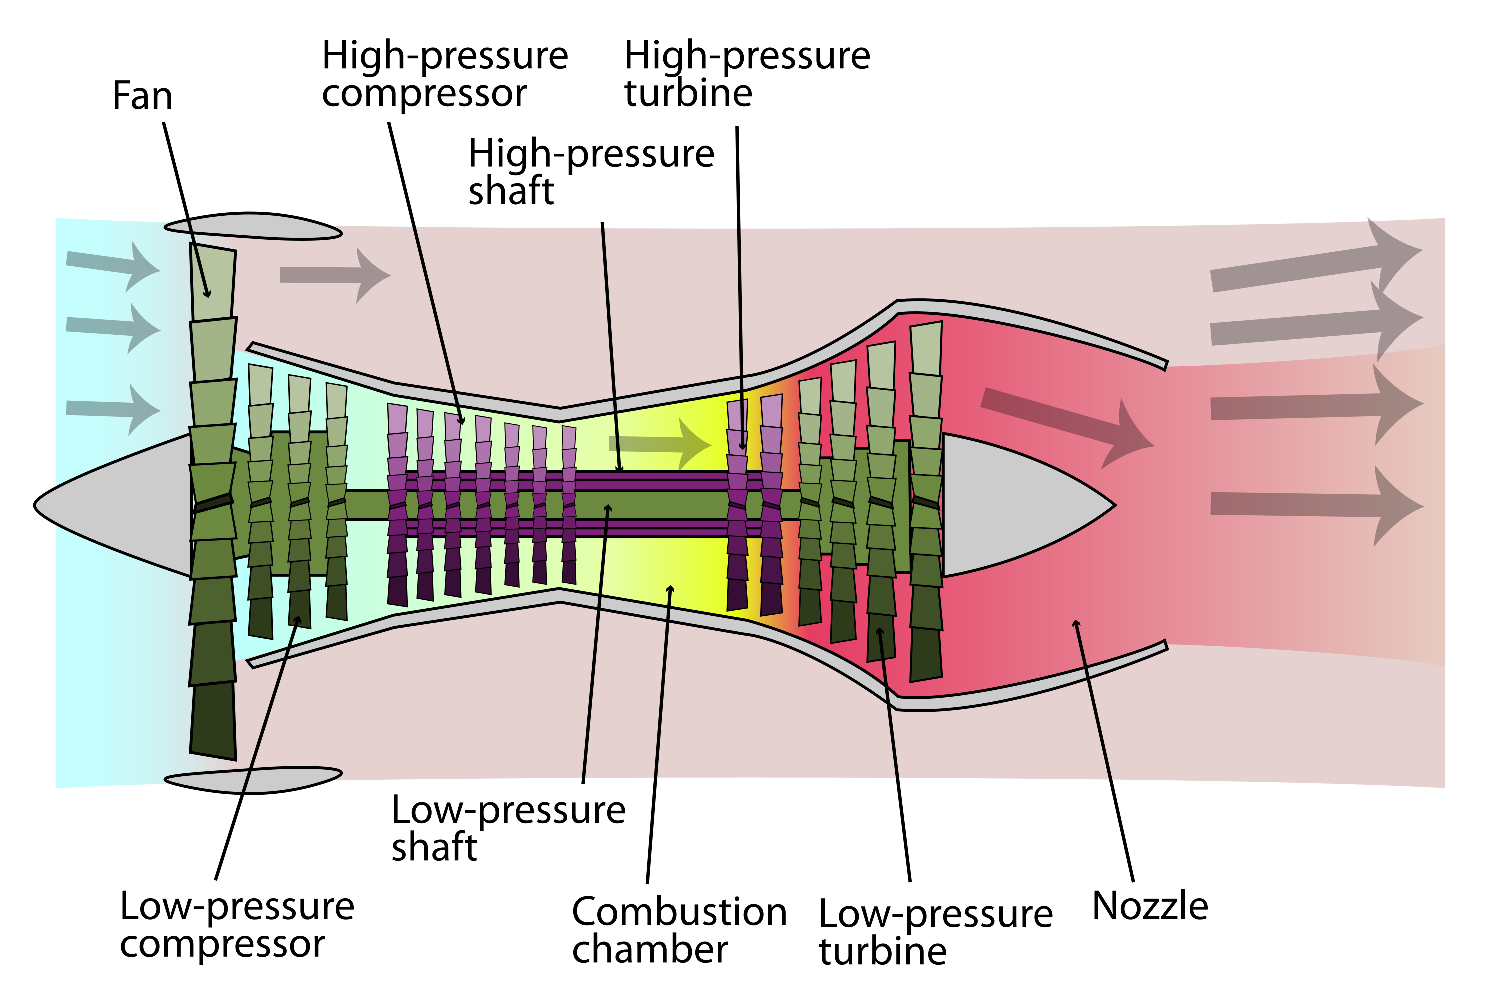
\includegraphics[width=0.75\textwidth]{images/intro/Turbofan_operation}
     \caption{Turbofan schematic representation. SOURCE: Wikipedia}
     \label{fig.intro2}
\end{figure}
This gas turbine engine is composed by a fixed casing and by several spools. Airflow passing through the fan and then in compressors, combustion chamber and turbines follows a Brayton cycle. Thanks to the excess of power produced by this cycle, the fan provides engine thrust. 
Engines on current turbofan-powered commercial aircraft are mounted on pylons, which keep the engines off the wings or fuselage in order to isolate the engine and airframe aerodynamic characteristics (c.f. figure \ref{fig.intro5}).
\begin{figure}[!ht]
	\centering   
	\includegraphics[width=0.75\textwidth]{images/intro/pylon_location}
	\caption{Commonly adopted pylon position in large turbofan propelled aircraft. Source: \cite{ASDM}} 
	\label{fig.intro5}
\end{figure}
The pylons must transmit the thrust loads from the engine to the airframe as well as convey all fluid and electrical
interconnections. 
\begin{figure}[!ht]
	\centering   
	\includegraphics[width=0.75\textwidth]{images/intro/pylonA340}
	\caption{Pylon structure (A340 example). Source: \cite{ASDM}} 
	\label{fig.intro6}
\end{figure}
Among pylon substructures (c.f. figure \ref{fig.intro6}), primary structure transfers engine loads to the wing. This is ensured by a system of connections between pylon and engine or wing (so called engine and wing mounts respectively) and by the pylon torque box that joins these two. The engines are enclosed by fairings known as nacelles (c.f. figure \ref{fig.intro7}), which contain many of the subsystems
important to the operation of the aircraft such as the electrical generators. The nacelles also serve other purposes,
including aerodynamic fairing of the engine, conditioning of airflow into the engine, thrust reversing, and noise
attenuation. The aerodynamic, structural, and subsystem integration of the engine and nacelle with the airframe are
important to determine aircraft performance and optimum engine characteristics such as propulsor diameter and
fan pressure ratio. \clearpage
\begin{figure}[!ht]
	\centering   
	\includegraphics[width=0.75\textwidth]{images/intro/nacelle}
	\caption{Nacelle subsystems. Source: \cite{ASDM}} 
	\label{fig.intro7}
\end{figure}
\marginnote{\textsl{Increasing the Bypass Ratio}}[1cm]
To improve the existing propulsion efficiency several technologies are currently investigated \cite{national2016commercial}. One of those consists in increasing the so called bypass ratio. This is defined as the ratio between the airflow passing through the fan and then ejected from the fan nozzle (which mainly contributes to engine thrust) and the airflow passing through the combustion chamber (responsible for power generation).   
Increasing turbofan bypass ratio has the following consequences on design and performances:
\begin{itemize}
\item Fan diameter needs to be increased. As a consequence, the propulsion efficiency is also improved. In fact for the same level of thrust provided by the fan, outlet air velocity  can be reduced, consequently reducing losses and noise. 
\item Core diameter needs to be decreased. This is because aircraft propulsive efficiency is improved and that means that less power is demanded for the same level of engine thrust. Moreover this is also needed to improve thermodynamic efficiency when the temperature and pressure in the first stage of turbine are increased. \cite{national2016commercial}. 
\end{itemize}
Engine and integration design are challenged by these drivers for several reasons. \marginnote{\textsl{Tip-clearance variation challenge}}[1cm] Among others, such designs have to deal with larger engine deformations that can deteriorate the control of stator to rotor blade  tip clearances, defined as the radial gap between the rotor blade tips and the engine casing. In fact a larger engine will be subjected to larger loads and eventually to larger deformations. On top of that the center of gravity of the engine is moved forward possibly amplifying the effect of inertial loads. An appropriate sizing needs to be considered in order to avoid excessive closures or openings.
An abradable coat material is often applied to the engine casing. 
 This sacrificial material is often milled by the rotor due to engine deformations that can close these gaps. When this happens, the aerodynamic performance of the stage is reduced, increasing the overall engine specific fuel consumption. Moreover, to keep the same level of thrust, more fuel needs to be injected in the combustion chamber consequently increasing the temperature of outlet gas. Engine material can then be subjected to high temperature corrosion phenomena that reduce the engine time on wing \cite{lattime2002turbine}. In compressor stages these gaps have even more severe consequences since surge margin is reduced. This means that not only fuel consumption is affected, but also safety and engine operability \cite{benito20083d}. Also in the fan stage the openings reduce the propeller efficiency further impacting the specific fuel consumption.\\
\marginnote{\textsl{Tip-clearance drivers}}[1cm]  
Tip clearance variations in both compressor and turbine stages can be due to both  engine loads (propulsion induced) and flight loads. Engine loads include centrifugal, thermal,
internal engine pressure, and thrust loads. Flight loads
include inertial (gravitational), aerodynamic (external
pressure), and gyroscopic loads. Engine loads can
produce both axisymmetric and asymmetric clearance
changes (see Figures \ref{fig.intro3} and \ref{fig.intro4}). Flight loads produce
asymmetric clearance changes \cite{lattime2002turbine}. 
\begin{figure}[!ht]
\centering   
 \includegraphics[width=0.5\textwidth]{images/intro/axisym_tip}
     \caption{Axisymmetric clearance variations} 
     \label{fig.intro3}
\end{figure}
\begin{figure}[!ht]
\centering   
 \includegraphics[width=0.5\textwidth]{images/intro/asym_tip}
     \caption{Asymmetric clearance variations} 
     \label{fig.intro4}
\end{figure}
Axisymmetric variations are mainly driven by engine rotor and stator sizing and by operating conditions. Nacelle and pylon are both linked to the engine. This means that their stiffness can have an impact on loads passing through each interface with the engine, therefore on the engine deformations. As a direct consequence pylon and nacelle design has an impact on tip clearance variation.\cite{lattime2002turbine}.  This contribution to the overall tip clearance variation in classic turbofan engine represents about a third of the total variation induced by other sources \cite{lattime2002turbine}. Nevertheless the relative importance of such contribution is still to be quantified for Ultra High Bypass Ratio (UHBR) architectures (Bypass ratio of the order of 30).\newpage
\marginnote{\textsl{A design problem}}[1cm] 
 The investigations that was conducted here, consist in studying how design choices made on:
 \begin{itemize}
 \item Engine outer casing main structure
 \item Engine to wing load path
 \item Nacelle and pylon main structure
 \end{itemize}
affect engine tip clearance variations in the context of UHBR architecture. For the aforementioned considerations such designs could be beneficial for both $CO_2$ emissions, engine life and safety. 
 In the determination of such a design one should be able to estimate the performance, in terms of tip clearance variation control and select a design considered 'best' among others.\\ 
 \marginnote{\textsl{Simulation driven design}}[1cm]
 Using only engineering considerations in the context of such complex phenomena could possibly be misleading or insufficient. For this reason an automated procedure, based on optimization algorithms in combination with a simulation model are proposed. A mathematical description of each configuration is then required and corresponding models should be available. In particular, structural optimization approaches deal with mechanical responses and often try to achieve the lightest or the stiffest design responding to some strength requirements on the solution. \\
 \marginnote{\textsl{Why Topology Optimization?}}[1cm] Depending on the design mathematical description, the optimal solution is more or less driven by the modeling choice made on the solution. In the industrial problem considered by this study, assumptions made on the connectivity between pylon and engine can drive the solution to configurations that one cannot ensure to be optimal.  For this reason a way of considering a large spectrum of possible solutions is by addressing the problem in a topology optimization framework. 
\section*{Topology Optimization approaches}
 Topology optimization is a powerful tool that can be used to explore structural design. The inputs for topology optimization are the geometry of the design zone (i.e. a region in the space delimitating the structure), boundary conditions and materials. A structural model (often a Finite Element model) is generated to compute each configuration's responses. 
The formulation can then be stated, in the form of a non-linear constrained optimization problem. This means that a model response is selected as objective to be minimized or maximized and other responses are constrained.
For what concern the design variables, a general distinction can be made at this level:
\begin{itemize}
\item The design variables are associated to the presence or the absence of material, at a given point/element in the space. These approaches are referred to as Eulerian in this work \cite{zhang2016lagrangian}, in reference to the continuum mechanics and the representation of displacements. In this first family one can find more common density based approaches \cite{bendsoe1989optimal,zhou1991coc,bendsoe1995optimization},  Level Set approach \cite{wang2003level,allaire2004structural} and ,  evolutionary approaches \cite{xie1993simple,xia2018bi}. 
\item The design variables are associated with geometric properties of features that are assembled to obtain the final solution.  This second family are referred to as Lagragian or explicit approaches \cite{zhang2016lagrangian}. Classic examples are the Moving Morphable Components approach (MMCs) \cite{guo2014doing,guo2016explicit,zhang2016new,zhang2017new}, the Moving Morphable Voids (MMVs) \cite{zhang2017explicit}, the Geometry Projection Method (GP) \cite{bell2012geometry,norato2015geometryde,zhang2016geometry}, the Method of Moving Morphable
Bars (MMB) \cite{hoang2017topology} and  the Moving Node Approach (MNA) \cite{overvelde2012moving}. 
\end{itemize}
In both cases design variables are constrained by lower and upper bounds. Once that the optimization problem is stated, gradient based optimization algorithms are typically employed to improve an initial guess design. When a solution is determined, in both cases the solution has to be interpreted in terms of geometry, manufacturing technology and advanced design considerations. Further optimizations (shape and sizing) are often casted to obtain sized designs that respect reserve factors (i.e. safety factors). In \cite{zhu2016topology} one can find an up to date review of the most promising applications of topology optimization to aerospace structures. Topology optimization has shown its advantages for the design of aircraft parts like the wing internal primary structure \cite{eves2009topology,aage2017giga}, the wing-box, fuselage \cite{niemann2013use,singh2016topology} and of the pylon \cite{remouchamps2011application,xue2012structural}.  
\section*{PhD goals}
\marginnote{\textsl{Engine-wing load path determination}}[1cm]
As aforementioned the load path between engine and wing, is a contributor to engine performance and in particular fuel consumption. Note that there are larger contributors to the engines’ performances which are exclusively dependent on the engine manufacturer's design choices. However the engine's attachment to the wing and the resulting load path, is a significant contributor to the performance while being mainly a design choice of the aircraft manufacturer.
Physical intuition can be effective in this choice, only for very simple considerations. On the other hand to prevent complex phenomena like engine casing ovalization, physical intuition is often misleading. For this reason simulation should be used as an exploration tool to get rid of bad solutions and select promising configurations. To address such a complex problem, without making too strong hypotheses on the solution's connectivity, a topology optimization strategy is investigated in the present work. 
\marginnote{\textsl{Research axes}}[1cm]
In this PhD topology optimization framework is developed, initially intended to use Eulerian approaches and successively adapted for Lagrangian approaches to address this design problem. Eulerian approaches are able to represent organic designs that can be considered as reference solutions, even if not attainable by nowadays manufacturing technologies. Lagrangian approaches on the other hand make an assumption on the basic components that should compose the solution. For this reason their power of representation is restrained, but their advantage is their link with an explicit geometry representation. This can both decrease the overall optimization computational effort and the end to end design effort.
The following challenges should then be addressed in order to deal with the engine-to-wing attachment design problem:
\begin{enumerate}
\item The proposed framework should be able to deal with industrial engine finite element models allowing also the post-processing of tip clearance variations. Such models are often provided in industrial finite element software like Nastran or Abaqus. An efficient interface with such programs should be therefore provided.
\item Complex geometries of the design zone may require at least non uniform meshes. In fact due to aerodynamic needs and also to the kinematic interfacing with the engine and design region models, voxel meshes should be avoided.  
\item  Finite element simulations including inconsistent mesh interfaces between models should be allowed. The engine model being provided by the engine manufacturer comes in a given discretization. To avoid constraints on design region discretization the provided framework should be able to connect non consistent discretizations.
\item  Efficiency and scalability should be implementation drivers as the resolution of 3D topology optimization problems can quickly become prohibitive. In fact reducing finite element mesh size the computational burden associated with both analysis and optimization is increased. The provided framework should therefore employ adapted techniques for both.  
\item The possibility to consider stress based topology optimization. In fact most topology optimizations are concerned with  structural stiffness. On the other hand the stiffest design is not always the strongest. Dealing with stress problem is challenging and the provided framework should adopt appropriate techniques. 
\item The use of Lagragian approaches in topology optimization. A shortcoming of Eulerian approaches is their lack of an explicit control on the final solution geometry, often requiring human intervention and solution simplifications to provide an acceptable design. Lagrangian approaches provide an efficient solution to this issue and should therefore be provided by the proposed framework.
\item The introduction of explicit geometric constraints linked to the product to be designed. In fact another advantage of Lagrangian approaches is the possibility to use constitutive components that can make easier the determination of a manufacturing process for the solution. The proposed framework will allow this investigation.
\end{enumerate}
At the best of the author's knowledge at the beginning of this project there wasn't any industrial or academic framework that could provide a satisfactory answer to all these requirements. For this reason a novel topology optimization framework will be developed in this study.
The goal of this work can be resumed in this question:\\
\textit{Is it possible to identify disruptive design features of engine pylon and mounts architecture that have an impact on tip clearance variations?} 
\\
The question was investigated by the development of a novel topology optimization framework that had to provide effective solutions to the aforementioned challenges.
%\marginnote{\textsl{Programming Language Considerations}}[1cm]
 %Nevertheless existing libraries for finite element analysis and topology optimization provide a baseline for the development of the proposed framework.
 %Some features considered in this framework are nevertheless unique and were developed from scratch. For this reason Matlab programming language was considered despite computational efficiency possible implications. 
\section*{Layout}
The investigation of this work can be divided in 3 large topics that will be covered in this manuscript, the finite element analysis, the Eulerian topology optimization approaches and the Lagrangian topology optimization approaches.
As a consequence the reminder of this work is organized as follows:
\begin{itemize}
\item \textbf{Chapter \ref{chap:1}} deals with challenges related finite element analysis, state of the art approaches and proposed solutions are covered in this chapter.  The fundamentals of linear static analysis and finite element analysis are reviewed in section \ref{sec:1.1}. A representative use case engine finite element Model,  built for this work, is presented in subsection \ref{ssec1.2.1}. The post processing of tip clearances required to assess a performance analysis is also presented in subsection \ref{ssec1.2.2}.  In section \ref{sec1.3} some advanced techniques for the interface of non-consistent meshes (Mortar approach \cite{bernardi1989new}, Rescaled Localized Radial Basis function interpolation \cite{deparis2014rescaled} and Internodes \cite{deparis2016internodes}) are reviewed. Their shortcomings in terms of accuracy and complexity are treated with the introduction of novel techniques \cite{coniglio2018weighted}. To deal efficiently with an industrial engine model, static condensation and superelement exploitation was reviewed \ref{subsection1.4.1}. Finally to efficiently solve the system of balance equations, efficient multigrid preconditioners for iterative solvers are reviewed and benchmarked on a 3D finite element model in subsection \ref{subsection1.4.2}. 
\item \textbf{Chapter \ref{chap:2}} deals with challenges encountered in structural topology optimization by the use of the Solid Isotropic Material with Penalization (SIMP) approach. Simulation driven design is reviewed in section \ref{sec:2.1} as the mathematical formulation of SIMP topology optimization in section \ref{sec:2.2}. Constraint aggregation and relaxation techniques are reviewed to deal with stress based topology optimization formulations in section \ref{Sec2.3}.
In section \ref{SIMP_application} the SIMP application to pylon and engine mount design is presented.
\item \textbf{Chapter \ref{chap:3}} deals with challenges encountered in structural topology optimization by the use of Lagrangian approaches. Moving Morphable Components, Geometry Projection Method, Moving Node Approach are firstly reviewed in sections \ref{MMC}, \ref{GP} and \ref{MNA} respectively. A new Generalized Geometry Projection approach is proposed as a generalization of existing techniques in section \ref{GGP}. Geometric assembly techniques are then reviewed in section \ref{GA}. Analytic derivatives computation is then provided in section \ref{SA}. The application to 2D usecase problems for both stiffness based and stress based formulations are provided in section \ref{I} and \ref{IS} respectively. Finally the application to the  engine pylon and mount design of a novel MNA-type approach is considered in section \ref{MNA_application}. 
\item \textbf{Chapter \ref{chap:4}}  outlines the main conclusions and the perspectives for the future research related to this work.
\end{itemize}

%%% Local Variables: 
%%% mode: latex
%%% TeX-master: "../phdthesis"
%%% End:

% % !TeX spellcheck = en_US
\chapter{Structural analysis by FEM }
\label{chap:1}
\minitoc
\begin{mdframed}[hidealllines=true,backgroundcolor=lightgray!20]
\section*{Résumé}
Dans le chapitre d'introduction nous avons relevé un besoins et un cahier des charges pour le cadre que l'on souhaite développer. Pour cela un modèle utilisable sera nécessaire pour prédire
\begin{itemize}
\item Les déformations d'un moteur intégré soumis à des chargements.
\item L'impact de ces déformations sur les "tip-clearance".
\item L'impact des variations de "tip-clearance" sur la consommation du moteur.
\end{itemize}
Dans un premier temps nous rappelons le bases de théorie de la mécanique des solides déformables. Ensuite la méthode des éléments fini est introduite comme moyen de construction de modèle. Une maquette éléments finis de moteur est introduite pour la prédictions des variations de "tip-clearance" et de performance moteur. Pour pouvoir traiter la communication entre maillage incohérent, une étude bibliographique est d'abord présentée et deux nouvelles contributions sont introduites. L'approche WACA essaye de fournir un bon compromis entre précisions, complexité et cout computationnel. L'approche de correction de moments fournie une technique d'amélioration de toutes les techniques existantes en imposant "apriori" la conservation du bilan des moments mécaniques à l'interface entre maillages. Ces techniques ont été implémentées et comparées avec différentes approches disponibles dans la littérature.
Étant le modèle de moteur intégré utilisé dans les prochains chapitres pour faire de l'optimisation topologique, son cout d'évaluation doit être contenu le plus possible. Une première approche proposée pour réduire le temps de calcul et pour gérer des modèles moteurs complexes consiste à utiliser des super-éléments. Cela nécessite l'utilisation de matrices fournies par les logiciels commerciaux. Pour cela nous faisons un rappel sur les étapes nécessaires à leur exploitation. Ensuite la méthode itérative du gradient conjugué avec preconditionneur multigrid géométrique est aussi implémentée et testés avec différents smoothers pour réduire les temps de calcul de l'analyse éléments finis du problème en étude. 
\end{mdframed}
\section{Finite elements method in structural analysis }
\label{sec:1.1}
Structural analysis is a major part in the design and validation phase in many industrial sectors. Its objective consists in predicting the structural integrity and performance of structures under different phases of the product life cycle.
The aircraft industry relies on structural analysis for both safety and performance purposes. A product is in fact the object of several phases of testing before its integration.
Experimental testing is the most expensive and time demanding part as it needs the construction of prototypes, with increasing levels of fidelity and cost with the development phase. Moreover sensors, actuators, and testing facilities are needed for the appropriate simulation of the product environment.
On top of that, correctly understanding test results requires time, experience and high-skilled profiles. 
For all these reason, experiments, even if necessary, have to be reduced as much as possible. For this reason numerical simulation is nowadays employed for helping both explaining test results and reducing the overall number of experiences. 
At the roots of this methods stand a solid knowledge of the physics governing a particular phenomenon that has to be studied. 
The continuum hypothesis is considered as satisfied when studying structures on length scales much greater than that of inter-atomic distances. 
The governing equation of continua can be mathematically described by systems of Partial Differential Equations (PDEs), where the unknowns are fields that represent the quantity of interest that one would like to know in any point of the space. 
Finite Element Modeling (FEM) is the most popular approximation method used to solve PDE problems in industrial applications.
FEMs can in fact provide:
\begin{itemize}
\item Models for structures and fluid mechanical behavior.
\item Models for the quantification of thermal exchange phenomena.
\item Models for the quantification of electromagnetic phenomena. 
\item Models that account for coupled multi-physics phenomena.
\end{itemize}
The main goal of the beginning of this chapter is to introduce notations associated with the finite element formulation for the linear elasto-static problem, notations which will be used throughout the rest of the thesis. The optimization responses needed in chapter \ref{chap:2} need the evaluation of both a mechanical finite element model (c.f. subsection \ref{ssec1.2.1}) and an engine performance index model (c.f. subsection \ref{ssec1.2.1}). The rest of the chapter provides details about the techniques required to consider inconsistent meshes, superelements and efficient iterative solvers that are required to speed-up the overall optimization elapsed time.

\subsection{Elastostatics equations - strong and weak form}\label{subsec:1.1.1}
We consider an elastic body described by a 3D domain $\Omega$ (cf. figure \ref{fig.1}). We denote its boundary, $\partial \Omega$ and the outward normal vector $\VectorVar{\hat{n}}$.
Finally we call $\partial \Omega_{u}$ and $\partial \Omega_{\sigma}$ the boundary where, respectively displacements and surface traction are prescribed, so that $\partial \Omega_{\sigma} \cup \partial \Omega_{u} =\partial \Omega $. We also considered the hypothesis that $\partial \Omega_{u} \cap\partial \Omega_{\sigma}=\emptyset$.\\
\begin{figure}[ht]
\centering
\includegraphics[width=8cm]{images/Ch1/solid}
\caption{linear elastostatics problem definition}
\label{fig.1}
\end{figure}
In elastostatics problems one seeks the displacement field $\VectorVar{u} \in H^1(\Omega)$ that solves the local balance, boundary conditions and constitutive equations\footnote{In this context we consider a 3D solid continuum so that $\VectorVar{u}\equiv \VectorVar{u,v,w}$.}:
\begin{eqnarray}
\label{eq.1.1}
\nabla \cdot \MatrixVar{\sigma} + \VectorVar{b}=\VectorVar{0}  & & \forall \VectorVar{x} \in \Omega/\partial \Omega \\
\label{eq.1.2}
\VectorVar{u}=\VectorVar{\bar{u}} & & \forall \VectorVar{x} \in \partial \Omega_{u}  \\
\label{eq.1.3}
\MatrixVar{\sigma}\cdot\VectorVar{\hat{n}}=\VectorVar{\bar{t}} & & \forall \VectorVar{x} \in \partial \Omega_{\sigma}
\\
\label{eq.1.4}
\MatrixVar{\sigma}=\MatrixVar{\MatrixVar{E}}:\MatrixVar{ 	\varepsilon} & & \forall \VectorVar{x} \in \Omega
\end{eqnarray}
Where $\VectorVar{b}$ are the body force vector, $\MatrixVar{\sigma}$ is the stress tensor and $\nabla \cdot (\bullet)$ indicates the divergence operator, $\VectorVar{\bar{u}}$ and $\VectorVar{\bar{t}}$ are respectively the prescribed displacements field and surface force field defined on the boundary $ \partial \Omega_{\sigma}$ and $ \partial \Omega_{u}$, $\MatrixVar{\MatrixVar{E}}$ is the fourth order elastic tensor, $\MatrixVar{\varepsilon} = \VectorVar{\MatrixVar{D}} \cdot\VectorVar{u} $ is the infinitesimal strain tensor ($\VectorVar{\MatrixVar{D}}$ denotes the symmetric gradient operator), $\cdot$ stands for the scalar product and $:$ represents the double index contraction. \footnote{In this text we denote vectors quantity in braces, Matrix in brackets and third or fourth order arrays as Vectors of Matrices and as Matrices of Matrices, i.e. using nested braces and brackets.}\\

In order to use a finite element approach to discretize the elastostatics equations, a weak form of equation \eqref{eq.1.1} is introduced.
By evaluating the scalar product of equation \eqref{eq.1.1} with a compatible virtual displacement $ \VectorVar{v} \in \mathbb{V}$ and integrating it over the domain $\Omega$, the weak or integral formulation is obtained:
\begin{eqnarray}
\label{eq.1.6}
\int_{\Omega}{\VectorVar{v} \cdot (\nabla \cdot \MatrixVar{\sigma} + \VectorVar{b}) d\Omega}=\VectorVar{0} \quad \forall \VectorVar{v} \in \mathbb{V} 
\end{eqnarray}
Using the following identity, valuable for any differentiable field $\VectorVar{\alpha}$ and for any differentiable tensor $ \MatrixVar{\beta}$ :
\begin{equation}
\label{eq.1.7}
\nabla \cdot (\VectorVar{\alpha} \cdot \MatrixVar{\beta})=\nabla \VectorVar{\alpha} : \MatrixVar{\beta}+\VectorVar{\alpha}\cdot(\nabla \cdot \MatrixVar{\beta})
\end{equation}
Equation \eqref{eq.1.6}  becomes:
\begin{eqnarray}
\label{eq.1.8}
\int_{\Omega}{(\nabla \cdot (\VectorVar{v} \cdot \MatrixVar{\sigma}) - \nabla \VectorVar{v} :\MatrixVar{\sigma}  + \VectorVar{v} \cdot \VectorVar{b}) d\Omega}=\VectorVar{0} \quad \forall \VectorVar{v} \in \mathbb{V} 
\end{eqnarray}
Using the divergence theorem and taking the tensor product term to the right hand side one can get:
\begin{eqnarray}
\label{eq.1.9}
\int_{\partial \Omega}{(\VectorVar{v} \cdot \MatrixVar{\sigma}\cdot\VectorVar{\hat{n}} )d\partial \Omega}+\int_{\Omega}{(\VectorVar{v} \cdot \VectorVar{b}) d\Omega}=\int_{\Omega}{(\nabla \VectorVar{v} :\MatrixVar{\sigma}) d\Omega} \quad \forall \VectorVar{v} \in \mathbb{V} 
\end{eqnarray}
Finally using equations \eqref{eq.1.2} to \eqref{eq.1.4}.
\begin{eqnarray}
\label{eq.1.10}
\int_{\partial \Omega_{\sigma}}{\VectorVar{v} \cdot \VectorVar{\bar{t}} d\partial \Omega}+\int_{\Omega}{\VectorVar{v} \cdot \VectorVar{b} d\Omega}=\int_{\Omega}{\VectorVar{\MatrixVar{D}}\cdot \VectorVar{v} :\MatrixVar{\MatrixVar{E}}:\VectorVar{\MatrixVar{D}}\cdot \VectorVar{u}  d\Omega} \quad \forall \VectorVar{v} \in \mathbb{V}
\end{eqnarray}
Being both $\MatrixVar{\sigma}$ and $\MatrixVar{ 	\varepsilon}$ symmetric, the right hand side of equation \eqref{eq.1.10} can be simplified with the help of the following vectors:
\begin{eqnarray}
\VectorVar{\varepsilon}=\left\lbrace \begin{array}{c}
\varepsilon_{xx}\\ \varepsilon_{yy}\\ \varepsilon_{zz}\\ \gamma_{xy} \\ \gamma_{xz}\\ \gamma_{yz}
\end{array} \right \rbrace=\left\lbrace \begin{array}{c}
\frac{\partial u}{\partial x}\\ \frac{\partial v}{\partial y}\\ \frac{\partial w}{\partial z}\\ \frac{\partial u}{\partial y}+\frac{\partial v}{\partial x} \\ \frac{\partial u}{\partial z}+\frac{\partial w}{\partial x}\\ \frac{\partial v}{\partial z}+\frac{\partial w}{\partial y}
\end{array} \right \rbrace = \nabla_{sym}\VectorVar{u} ;\quad \VectorVar{\sigma}=\left\lbrace \begin{array}{c}
\sigma_{xx}\\ \sigma_{yy}\\ \sigma_{zz}\\ \tau_{xy} \\ \tau_{xz}\\ \tau_{yz}
\end{array} \right \rbrace
\end{eqnarray}
The generalized Hook's law equation \eqref{eq.1.4} can then be written for isotropic materials as:
\begin{equation}
\VectorVar{\sigma}=E \MatrixVar{\begin{array}{cccccc}
	C_1 & C_2 & C_2 & 0 & 0 & 0\\
	C_2 & C_1 & C_2 & 0 & 0& 0 \\
	C_2 & C_2 & C_1  & 0 & 0& 0 \\
	0 & 0& 0& C_3 & 0 & 0 \\
	0& 0& 0& 0& C_3 & 0 \\
	0 & 0 & 0 & 0 & 0 & C_3
	\end{array}} \VectorVar{\varepsilon}=E\MatrixVar{D}\VectorVar{\varepsilon}
\end{equation}
Where:
\begin{eqnarray}
C_1=\frac{1-\upsilon}{(1+\upsilon)(1-2\upsilon)}; \quad C_2=\frac{\upsilon}{(1+\upsilon)(1-2\upsilon)}; \quad C_3=\frac{1}{2(1+\upsilon)}
\end{eqnarray}
$E$ and $\upsilon$ are the material's Young modulus and Poisson ratio respectively. Then equation \eqref{eq.1.10} can be written as :
\begin{eqnarray}
\label{eq.1.11b}
\int_{\partial \Omega_{\sigma}}{\VectorVar{v}^T \VectorVar{\bar{t}} d\partial \Omega}+\int_{\Omega}{\VectorVar{v}^T \VectorVar{b} d\Omega}=\int_{\Omega}{\left(\nabla_{sym}\VectorVar{v}\right)^T E\MatrixVar{D} \nabla_{sym}\VectorVar{u} d\Omega}\quad \forall \VectorVar{v} \in \mathbb{V}
\end{eqnarray}
\subsection{Discretization using finite element}\label{subsec1.1.2}
In the standard Galerkin formulation of the finite element method the space of the solution $\mathbb{U}$ and the space of test functions $\mathbb{V}$ are approximated by their discrete approximation: $\mathbb{U}^h$ and $\mathbb{V}^h$ that are given by the linear combination of shape functions defined in each element\footnote{The standard Galerkin approximation is a well-established approach that produces a symmetric stiffness matrix consistent with the classic variational formulation. More generally, the spaces of functions of $\mathbb{U}^h$ and $\mathbb{V}^h$ may not be the same, as it is the case for the Petrov-Galerkin methods. }. so that the test function and the displacement field can be approximated as follows:
\begin{eqnarray}
\label{eq.1.11}
\VectorVar{v}=\MatrixVar{N}^{(h)}\VectorVar{v}^{(h)} \qquad
\VectorVar{u}=\MatrixVar{N}^{(h)}\VectorVar{u}^{(h)}
\end{eqnarray}
In which $\VectorVar{v}^{(h)}$ and $\VectorVar{u}^{(h)}$ are the vectors containing the corresponding field values at each node for each degree of freedom, $\MatrixVar{N}^{(h)}$ is the $N_d \times N_dN$ matrix containing, $N_d$ is the number of DOFs per node, $N$ is the number of nodes of the discretization. Accordingly in a 3-D mesh with solid elements  $\MatrixVar{N}^{(h)}$ has the following structure:

\begin{equation}
\label{eq.1.12}
\MatrixVar{N}^{(h)}=\left[ \begin{array}{cccccc}
N_1\MatrixVar{I}_d&N_2\MatrixVar{I}_d& \cdots&N_j\MatrixVar{I}_d&\cdots&N_N\MatrixVar{I}_d
\end{array} \right]
\end{equation}
Where $\MatrixVar{I}_d$ is the $N_d \times N_d$ identity matrix and $N_j$ are the shape functions associated with the $j^{th}$ node. These functions are often chosen to be Lagrange basis polynomials defined on each finite element. For ease of implementation, FEA software makes the use of reference elements (c.f. figure \ref{fig.1a}) that renders the definition and the integration of shapes functions easier. 
\begin{figure}[!ht]
     \subfloat[ Reference element in the $(\xi,\eta,\zeta)$ space\label{fig.1a}]{%
       \includegraphics[width=0.5\textwidth]{code_matlab/reference_element.png}
     } 
     \subfloat[Corresponding mapped element in the $(x,y,z)$ space\label{fig.1b}]{%
       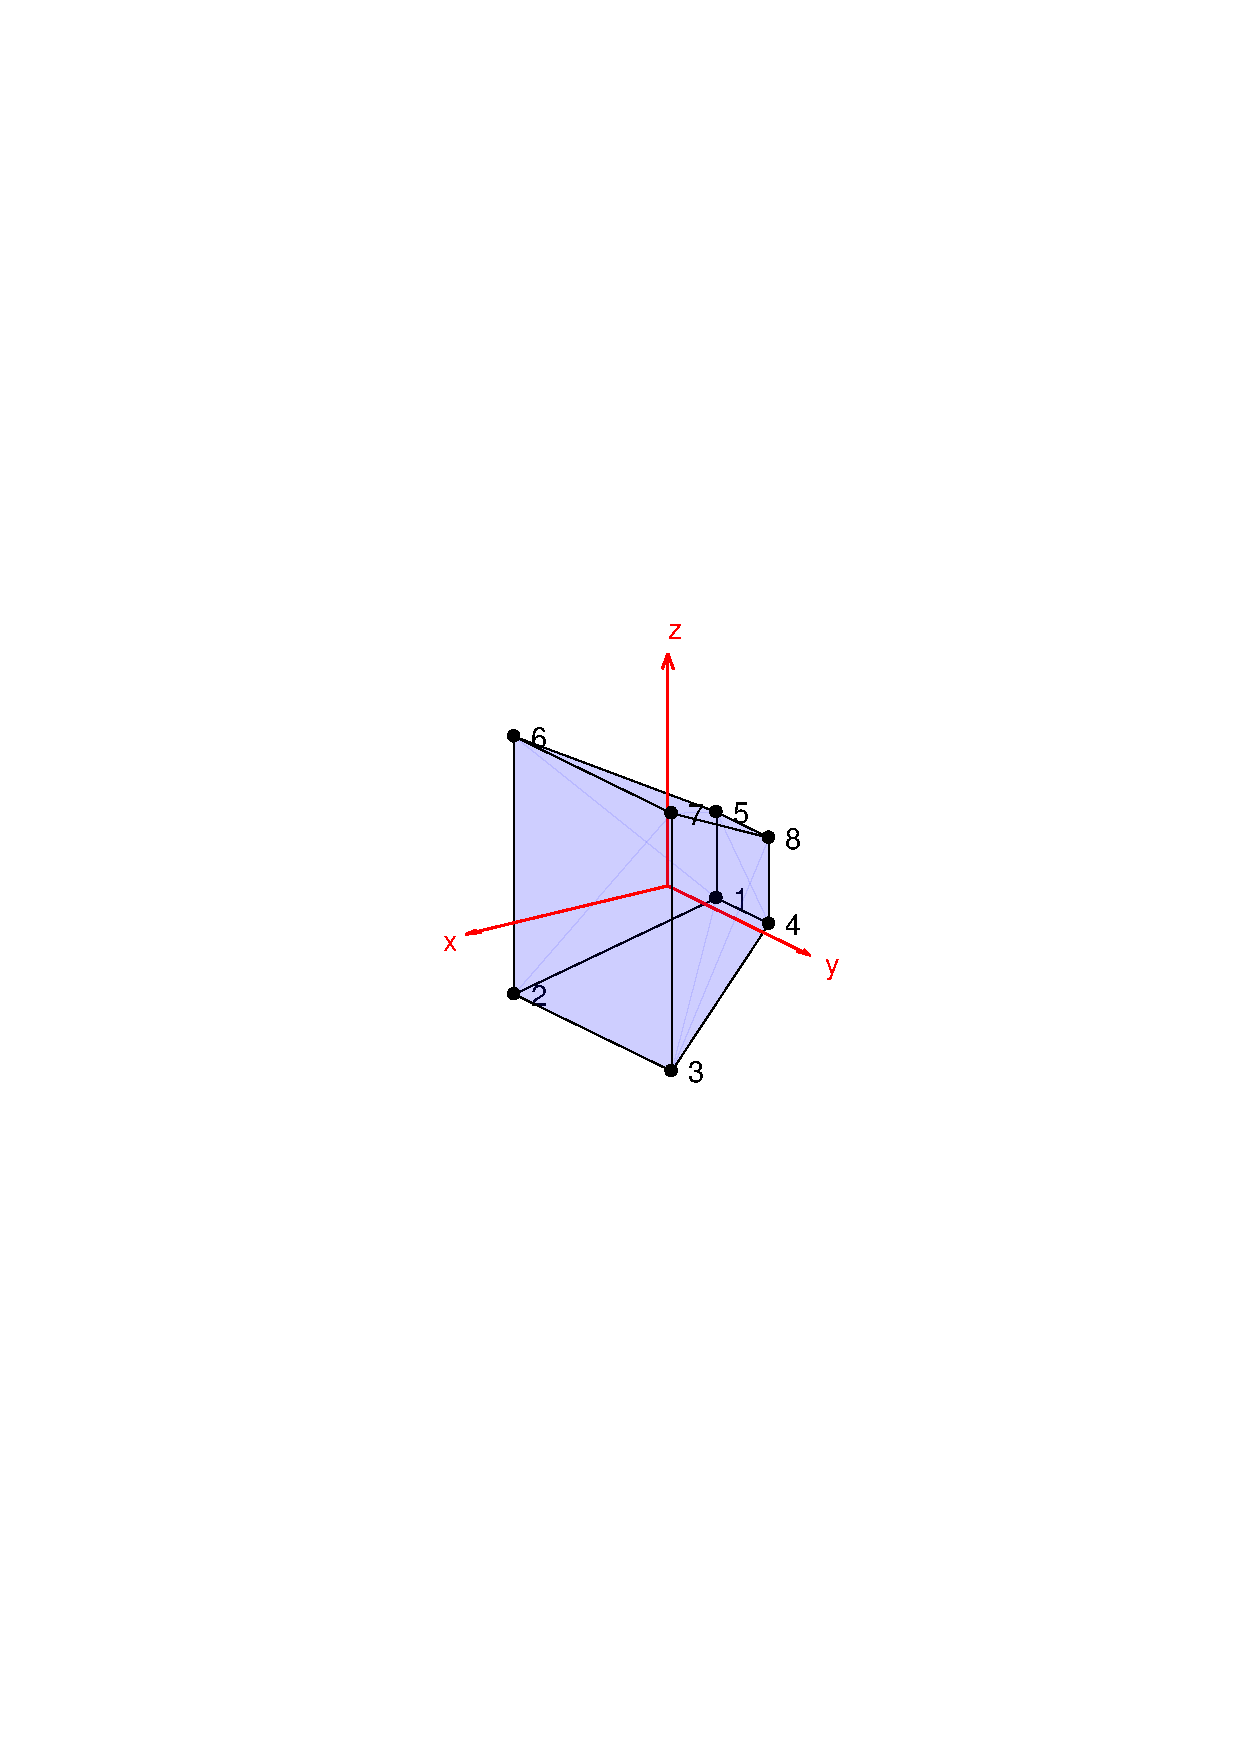
\includegraphics[width=0.5\textwidth]{code_matlab/mapped_element.png}
     }
     \caption{Classic Mapping in FEA}
     \label{fig.1.2}
   \end{figure}
The mapping between reference and actual geometry within a finite element is also made by the same shape functions as follows:
\begin{equation}
\label{eq.1.16}
\VectorVar{X_g}=\VectorVar{\begin{array}{c}
x\\y\\z
\end{array}}=\MatrixVar{\begin{array}{c}\VectorVar{x_n}^T\\\VectorVar{y_n}^T\\\VectorVar{z_n}^T\end{array}}\VectorVar{N_n(\xi,\eta,\zeta)}
\end{equation}
Where  $\VectorVar{x_n},\VectorVar{y_n},\VectorVar{z_n}$ are the column vectors containing the $x,y$ and $z$ coordinates of element nodes, and  $\VectorVar{N_n(\xi,\eta,\zeta)}$ is the column vector containing the value of shape functions relative to element nodes. 
To determine the form of the shape functions one can observe that putting in input the element node reference coordinates $\xi_i,\eta_i,\zeta_i$, for $i=1,2,...,N$, back  into equation \eqref{eq.1.16} one should find the corresponding nodal coordinates $x_i,y_i,z_i$. This means that all shape functions have to satisfy $N$ different interpolation conditions. For this reason, in the case of 8 node hexahedral elements, each shape function is chosen to have the following form:
\begin{equation}
N_i(\xi,\eta,\zeta)=\VectorVar{\begin{array}{cccccccc}
1&\xi&\eta&\zeta&\xi\eta&\xi\zeta&\eta\zeta&\xi\eta\zeta
\end{array}}\VectorVar{\begin{array}{c}
a_{i000}\\a_{i100}\\a_{i010}\\a_{i001}\\a_{i110}\\a_{i101}\\a_{i011}\\a_{i111}
\end{array}}=\VectorVar{p(\xi,\eta,\zeta)}^T\VectorVar{a_i}
\end{equation}
then one can also write:
\begin{equation}
\VectorVar{N_n(\xi,\eta,\zeta)}=\MatrixVar{\begin{array}{c}
\VectorVar{a_1}^T\\
\VectorVar{a_2}^T\\
\vdots\\
\VectorVar{a_8}^T
\end{array}}\VectorVar{p(\xi,\eta,\zeta)}=\MatrixVar{A}\VectorVar{p(\xi,\eta,\zeta)}
\end{equation}
To find the 64 coefficients of $\MatrixVar{A}$ one can employ the 8 interpolation conditions specific to each shape function:
\begin{equation}
\label{eq1.19}
\MatrixVar{\begin{array}{c}\VectorVar{x_n}^T\\\VectorVar{y_n}^T\\\VectorVar{z_n}^T\end{array}}=\MatrixVar{\begin{array}{c}\VectorVar{x_n}^T\\\VectorVar{y_n}^T\\\VectorVar{z_n}^T\end{array}}\MatrixVar{A}\MatrixVar{\begin{array}{cccc}
\VectorVar{p(\xi_1,\eta_1,\zeta_1)}&\VectorVar{p(\xi_2,\eta_2,\zeta_2)}&\cdots&\VectorVar{p(\xi_8,\eta_8,\zeta_8)}
\end{array}}
\end{equation}
Where $\xi_i,\eta_i,\zeta_i$ are nodal reference coordinates and can be obtained as the components of the following vectors:
\begin{eqnarray}
	\VectorVar{\xi}=\VectorVar{\begin{array}{c}
		-1\\1\\1\\-1\\-1\\1\\1\\-1
		\end{array}} \quad \VectorVar{\eta}=\VectorVar{\begin{array}{c}
		-1\\-1\\1\\1\\-1\\-1\\1\\1
		\end{array}} \quad\VectorVar{\zeta}=\VectorVar{\begin{array}{c}
		-1\\-1\\-1\\-1\\1\\1\\1\\1
		\end{array}}
\end{eqnarray}
To satisfy equation \eqref{eq1.19} one must have:
\begin{equation}
\MatrixVar{A}=\MatrixVar{\begin{array}{cccc}
\VectorVar{p(\xi_1,\eta_1,\zeta_1)}&\VectorVar{p(\xi_2,\eta_2,\zeta_2)}&\cdots&\VectorVar{p(\xi_8,\eta_8,\zeta_8)}
\end{array}}^{-1}
\end{equation}
Using the discretization of equation \eqref{eq.1.11}, the problem of equation \eqref{eq.1.10} can be written as the well-known system of equation:
\begin{equation}
\label{eq.1.13}
\MatrixVar{K}^{(h)}\VectorVar{u}^{(h)}=\VectorVar{f}^{(h)}
\end{equation}
Typically $\MatrixVar{K}^{(h)}$ and $\VectorVar{f}^{(h)}$ are called \textit{stiffness matrix} and \textit{load vector}. They are defined as:
\begin{eqnarray}
\label{eq.1.14}
{K}_{i,j}^{(h)}=\int_{\Omega}{\left(\MatrixVar{\nabla_{sym}N_i}^{(h)}\right)^T E\MatrixVar{D}\MatrixVar{\nabla_{sym}N_j}^{(h)}   d\Omega}\\
\label{eq.1.15}
{f}_{i}^{(h)}=\int_{\partial \Omega_{\sigma}}{(\MatrixVar{N_i}^{(h)} \cdot \VectorVar{\bar{t}} )d\partial \Omega}+\int_{\Omega}{(\MatrixVar{N_i}^{(h)}\cdot \VectorVar{b}) d\Omega}
\end{eqnarray}
Here the column vectors $\MatrixVar{N_i}^{(h)}$ and $\MatrixVar{N_j}^{(h)}$ are respectively the i-th and j-th column of $\MatrixVar{N}^{(h)}$.
The integrals of equations \eqref{eq.1.14} and \eqref{eq.1.15} can be decomposed as the sum of the integrals computed on each finite element: 
\begin{eqnarray}
{K}_{i,j}^{(h)}=\sum_{el=1}^{n_{el}}E_{el}\int_{\Omega_{el}}{\left(\MatrixVar{\nabla_{sym}N_i}^{(h)}\right)^T \MatrixVar{D}\MatrixVar{\nabla_{sym}N_j}^{(h)}   d\Omega_{el}}\\
{f}_{i}^{(h)}=\sum_{el=1}^{n_{el}}\int_{\partial \Omega_{\sigma}\cap\partial \Omega_{el} }{(\MatrixVar{N_i}^{(h)} \cdot \VectorVar{\bar{t}} )d\partial \Omega_{el}}+\int_{\Omega_{el}}{(\MatrixVar{N_i}^{(h)}\cdot \VectorVar{b}) d\Omega_{el}}
\end{eqnarray}
Where the Young's modulus was supposed to be uniform over each finite element.
 These integrals are usually evaluated by Gauss quadrature over each element.
The mapping of equation \eqref{eq.1.16} can then be employed:
 \begin{eqnarray}
 {K}_{i,j}^{(h)}=\sum_{el=1}^{n_{el}}E_{el}\sum_{k=1}^{N_{GP}}{\left(\MatrixVar{\nabla_{sym}N_{ik}}^{(h)}\right)^T \MatrixVar{D}\MatrixVar{\nabla_{sym}N_{jk}}^{(h)}\determinant{\MatrixVar{J_k}}\omega_k}\\
 {f}_{i}^{(h)}=\sum_{el=1}^{n_{el}}\sum_{l=1}^{n_{GP}} {(\MatrixVar{N_{il}}^{(h)} \cdot \VectorVar{\bar{t_l}} )\determinant{\MatrixVar{J_l}}\omega_l}+\sum_{k=1}^{N_{GP}}{(\MatrixVar{N_{ik}}^{(h)}\cdot \VectorVar{b_k}) \determinant{\MatrixVar{J_k}}\omega_k}
 \end{eqnarray}
Where the notation $\MatrixVar{\nabla_{sym}N_{ik}}$ means that the i-th column of the matrix containing $\MatrixVar{\nabla_{sym}N_{i}}$ is computed on the k-th Gauss point of the el-th element, $\omega_k$ refers to the integration weights of the Gauss-Legendre integration rule chosen to compute each integral. Moreover due to the variable change, the Jacobian determinant of the geometrical mapping $\determinant{\MatrixVar{J_k}}$ has to be computed in each Gauss point of each element in the FEM.
Jacobian determinant can be computed as:
\begin{equation}
\determinant{\MatrixVar{J}} =\determinant{\MatrixVar{\frac{\partial \VectorVar{X_g}}{\partial \xi},\frac{\partial \VectorVar{X_g}}{\partial \eta},\frac{\partial \VectorVar{X_g}}{\partial \zeta}}}=\determinant{\MatrixVar{\begin{array}{c}\VectorVar{x_n}^T\\\VectorVar{y_n}^T\\\VectorVar{z_n}^T\end{array}} \MatrixVar{A}\MatrixVar{\frac{\partial \VectorVar{p}}{\partial \xi},\frac{\partial \VectorVar{p}}{\partial \eta},\frac{\partial \VectorVar{p}}{\partial \zeta}}} 
\end{equation}
In this expression one can observe that both $\MatrixVar{A}$, and $\MatrixVar{\frac{\partial \VectorVar{p}}{\partial \xi},\frac{\partial \VectorVar{p}}{\partial \eta},\frac{\partial \VectorVar{p}}{\partial \zeta}} $ only depend on the reference element nodal coordinates and on the Gauss point position in the reference space and not on the nodal coordinates of the finite element.
For the expression of $\MatrixVar{\nabla_{sym}N_i}^{(h)}$ one can apply the definition of $\nabla_{sym}$ operator in equation \eqref{eq.1.10} to the i-th column of $\MatrixVar{N}^{(h)}$:
\begin{equation}
	\MatrixVar{\nabla_{sym}N_i}^{(h)}=\VectorVar{\begin{array}{c}
		\frac{\partial N_{1i}}{\partial x}\\\frac{\partial N_{2i}}{\partial y}\\\frac{\partial N_{3i}}{\partial z}\\
		\frac{\partial N_{1i}}{\partial y}+\frac{\partial N_{2i}}{\partial x}\\\frac{\partial N_{1i}}{\partial z}+\frac{\partial N_{3i}}{\partial x}\\\frac{\partial N_{2i}}{\partial z}+\frac{\partial N_{3i}}{\partial y}
		\end{array}}
\end{equation}
Where $N_{1i},N_{2i},N_{3i}$ indicate the first, the second and the third component of the i-th column of  $\MatrixVar{N}^{(h)}$.
Computing $\MatrixVar{\nabla_{sym}N_i}^{(h)}$ is a non-trivial operation since shape functions are expressed in terms of reference variables $(\xi,\eta,\zeta)$, that map through equation \eqref{eq.1.16} the $(x,y,z)$ space. So the inverse mapping between reference and geometric space is an implicit set of functions that often cannot be reversed explicitly. To compute the shape function derivatives with respect to space variable one can use Jacobian matrix definition \footnote{Jacobian matrix of the geometric mapping is nonsingular when finite elements are not twisted and have all distinct nodes}:
\begin{equation}
\MatrixVar{\frac{\partial N_{li}}{\partial x},\frac{\partial N_{li}}{\partial y},\frac{\partial N_{li}}{\partial z}}= 
\MatrixVar{J}^{-1}\VectorVar{\begin{array}{c}
	\frac{\partial N_{li}}{\partial \xi}\\\frac{\partial N_{li}}{\partial \eta}\\\frac{\partial N_{li}}{\partial \zeta}\end{array}} 
\end{equation}
Thanks to these relationships, the system of balance equation can be expressed in terms of a linear system of equations. This system is actually singular, in fact as a last step one needs to apply the boundary conditions (equation \eqref{eq.1.2}). For brevity we will here after refer to stiffness matrix as $\MatrixVar{\mathbf{K_{tot}}}$, to the load vector as $\VectorVar{f_{tot}}$ and to the displacement vector as  $\VectorVar{u}$:
\begin{equation}
\label{eq.1.32}
\MatrixVar{\mathbf{K_{tot}}}\VectorVar{u_{tot}}=\VectorVar{f_{tot}}
\end{equation} The load vector can actually be decomposed in two components: the external load vector $\VectorVar{F}$ coming from applied load and the reaction forces vector $\VectorVar{R}$ coming from the boundary conditions so that:
\begin{equation}
\VectorVar{f_{tot}}=\VectorVar{F}+\VectorVar{R}
\end{equation}
To apply the boundary conditions it is useful to adopt a partition of degrees of freedoms in two sets:
the set of constrained DOFs $\VectorVar{u_b}$ and the set of free DOFs $\VectorVar{u_f}$. According to this partition equation \eqref{eq.1.13} becomes:
\begin{eqnarray}
\label{eq.1.17}
\MatrixVar{\mathbf{K_{bb}}}\VectorVar{u_b}+\MatrixVar{\mathbf{K_{bf}}}\VectorVar{u_f}=\VectorVar{R_b}+\VectorVar{F_b}\\
\label{eq.1.18}
\MatrixVar{\mathbf{K_{fb}}}\VectorVar{u_b}+\MatrixVar{\mathbf{K_{ff}}}\VectorVar{u_f}=\VectorVar{R_f}+\VectorVar{F_f}
\end{eqnarray}
The reaction force is applied only on constrained DOFs so that $\VectorVar{R_f}=\VectorVar{0}$. If all rigid modes are constrained by the boundary conditions, then $\MatrixVar{\mathbf{K_{ff}}}$ is non-singular.
 In this case, the system of equations \eqref{eq.1.17}-\eqref{eq.1.18} can be solved with respect to the unknowns $\VectorVar{u_f},\VectorVar{R_b}$:
\begin{eqnarray}
\label{eq.1.19}
\VectorVar{u_f}=\MatrixVar{\mathbf{K_{ff}}}^{-1}\left(-\MatrixVar{\mathbf{K_{fb}}}\VectorVar{u_b}+\VectorVar{F_f}\right)\\
\label{eq.1.20}
\VectorVar{R_b}=\MatrixVar{\mathbf{K_{bb}}}\VectorVar{u_b}+\MatrixVar{\mathbf{K_{bf}}}\VectorVar{u_f}-\VectorVar{F_b}
\end{eqnarray}
Another way of dealing with boundary conditions that can be more suitable for Multi-Grid solver is replacing the rows relative to constrained DOFs directly with the corresponding kinematic constraint equations.
To keep stiffness matrix symmetry for non-homogeneous Boundary Conditions, the term  $\mathbf{K_{fb}}\VectorVar{u_b}$ has to be considered directly in the right hand side.
\begin{eqnarray}
\label{eq.1.17s}
\MatrixVar{\mathbf{A_{bb}}}\VectorVar{u_b}=\VectorVar{b_b}\\
\label{eq.1.18s}
\MatrixVar{\mathbf{K_{ff}}}\VectorVar{u_f}=\VectorVar{F_f}-\MatrixVar{\mathbf{K_{fb}}}\VectorVar{u_b}
\end{eqnarray}
Note that for simple clamping conditions $\MatrixVar{\mathbf{A_{bb}}}$ is the identity matrix and $\VectorVar{b_b}=0$  so that also $\MatrixVar{\mathbf{K_{fb}}}\VectorVar{u_b}$ is zero.
The advantage of this alternative formulation is that the kinematic constraints are directly included in the global stiffness matrix, making it easier to make the transfer among discretization levels for multigrid solvers, as it will be discussed later in this chapter.
In most of commercial software a post processing can be applied to compute both the deformation field and the stress field on each finite element of the FEM. To do that one needs to apply equation \eqref{eq.1.10} and \eqref{eq.1.11}. As the shape functions are $C^0$ function, their derivatives are actually discontinuous passing from a finite element to the other. Moreover it has been shown that stress and deformations computed through the FEA are the most accurate when computed at the Gauss Points \cite{zlamal1978superconvergence,zhang2006natural}. For this reason in the preprocessing phase, when the stiffness matrix and the load vector are assembled, the following matrixes are commonly stored to be reused in the post processing phase:
\begin{eqnarray}
\label{eq.1.40}
	\VectorVar{\varepsilon}=\MatrixVar{B_{gp}}\VectorVar{u_{el}} \quad
	\VectorVar{\sigma}=\MatrixVar{D}\MatrixVar{B_{gp}}\VectorVar{u_{el}}
\end{eqnarray}
Where $\MatrixVar{B_{gp}}$ is a $6\times 24$ matrix called stiffness-displacement as it links the value of deformations in a given Gauss point with $\VectorVar{u_{el}}$ that indicates the $24\times1$ vector of DOFs for the corresponding element.
\section{A generic engine FEM for fuel consumption variation computation}
As discussed in the introduction, to compute the effect of a given design structure on tip clearance variation control, one needs to consider a mechanical model of the engine, nacelle and pylon (that hereafter we can also describe as Power-Plant System (PPS)). This requires to build the model of each component and then to assemble them together.
In this section we first introduce the engine finite element model employed as demonstrator. Then the post processing steps needed for the computation of a global performance index with respect to tip clearance variation is introduced. This will be described as thrust specific fuel consumption variation due to its link to the actual engine performance deterioration, induced by clearance variation. The reader can also observe that for the reasons discussed in the introduction, this parameter is also correlated to other issues such as engine life and operability.
\subsection{Structural Model}
\label{ssec1.2.1}
The mechanical behavior of both engine and PPS structure is usually studied using a Finite Element Model, integrating complex load combinations. Here we introduce a generic engine model that will be used throughout this work (c.f. figure \ref{enginewem}). 
\begin{figure}[hbt!]
\centering
\includegraphics[width=1\textwidth]{images/Ch1/enginegeometry}
\caption{Proposed Whole Engine Model (WEM). Colors identify zone with different properties. The connection between rotor and stator is represented by rigid connections at bearing locations.\label{enginewem}}
\end{figure}
This model is a simplification of an industrial engine model that in general can have a fan casing structure, a core casing structure and multiple shafts for rotors. The following assumptions are made regarding the model's mechanical behavior. Rotor shafts are modeled using just one beam model. Both fan casing and core casing are represented using shell models. Different properties are employed for each engine module casing. The connection between rotor and stator is made through four rigid connections that represent stator vane and bearing housing in the engine. Outlet guide vanes which connect the core casing to the fan casing are represented with radial beam model tied to each interface of the engine. The thermal and centrifugal expansion of rotor blades are not considered in our analysis and nonlinearities are neglected. Only aerodynamic loads linked with the aircraft maneuvers are considered for simplicity. These loads are applied statically. A general 3D solid design zone is integrated between the wing and the engine (see gray elements in figure \ref{f.1}). This is the zone where the topology optimization will need to find the optimal material placement. For simplicity and since this does not have a significant effect on optimization, we did not consider the air inlet and the nacelle structure.  The engine core casing and the design zone meshes are tied at specific region of compressor and turbine casing. For this reason the solution of the topology optimization problem will be connected to the engine at these same regions. This will avoid solutions connected on prohibited region such as the combustion chamber casing. The techniques employed for the connection between engine casing and design zone mesh will be detailed in section \ref{sec1.3}.
\begin{figure}[hbt!]
\centering
\includegraphics[width=1\textwidth]{images/Ch1/FEM_intro.eps}
\caption{\label{f.1} Engine and design zone (in gray) finite element model. The engine model is made of 9976 finite elements, 9312 linear quadrilateral elements of type and 664 beam elements. The solid design zone is clamped at the orange points representing a clamping to the wing.}
\end{figure}
Eight node brick elements were used to mesh the design zone and full eight points integration was employed for elementary stiffness matrix and stress evaluation. The design zone model is clamped at the wing interface position. The axial load on the engine is applied with concentrated forces on the shaft nodes and with distributed loads on the engine casing. Vertical and lateral loads are distributed uniformly on the circumference of fan stage. % The connection between shaft node and engine casing nodes at bearing positions are modeled using rigid Kinematic couplings i.e. rigid connections. 
The commercial software Abaqus 13.2 was employed for mesh generation and load case application.
\subsection{Performance Model}
\label{ssec1.2.2}
The performance function that we considered in this work is a simplification of the real Thrust Specific Fuel Consumption (TSFC) variation induced by the considered loading conditions. Engine fuel consumption could be impacted in different ways by the pylon and casing design. Here we only considered the effect of closures variations.
The tip clearance variation is described in figure \ref{f.2}, and defined in equation \eqref{eq.1}.
  \\
  \begin{figure}[hbt!]
  \centering
       \subfloat[ \label{f.2a}]{%
         \includegraphics[width=0.4\textwidth]{images/Ch1/tip_def1.eps}
       }
       \subfloat[\label{fig.2b}]{%
         \includegraphics[width=0.4\textwidth]{images/Ch1/tip_def2.eps}
       }
       \caption{Rotor and stator displacements under maneuvers loads: (a) $z-y$ engine section diagram for a given rotor stage. The red structure stands for the rotor, the blue curve for the deformed stator. (b) diagram illustrating radial displacement effect.
       The resulting tip clearance is the sum of the initial clearance $\delta_0$ and its variation induced by the engine deformation $\delta(\theta)$ }
       \label{f.2}
     \end{figure}
  \\
\begin{equation}
\label{eq.1}
\delta(\theta)=u_r^c(\theta)-u_r^b(\theta)=\lbrace r( \theta ) \rbrace^T \cdot \left( \lbrace u^c(\theta) \rbrace-\lbrace u^b(\theta) \rbrace\right)
\end{equation}
Where $u_r^c(\theta)$ and $u_r^b(\theta)$  are the radial displacements of casing and rotor blade tip respectively at the angular position $\theta$ and $\lbrace r( \theta ) \rbrace$ is the radial unit vector at the angle $\theta$ .
Considering an angular discretization of the circumference given by the stator mesh in the $s^{th}$ engine stage, $\theta^i_{(s)}$ the tip clearance variation at the angular section $i$ is then:	
\begin{equation}
\lbrace\delta_{(s)}\rbrace_i=\lbrace r( \theta^i_{(s) } \rbrace^T \cdot \left( \lbrace u^c(\theta^i_{(s)} \rbrace-\lbrace u^b(\theta^i_{(s)} \rbrace\right)
\end{equation}
That is actually a system of linear relationships that can be expressed in the matrix form:
\begin{equation}
\label{e.3}
\lbrace\delta_{(s)}\rbrace =\left[ \gamma_{(s)} \right] \lbrace U \rbrace
\end{equation}
where $\lbrace U \rbrace$ is the displacements vector.
To characterize a stage's contribution to the overall engine performance, tip-clearance's variation Root Mean Square (RMS) is evaluated at each stage:
\begin{equation}
\label{e.4}
R_{(s)} =\sqrt{\frac{\lbrace\delta_{(s)}\rbrace^T\lbrace\delta_{(s)}\rbrace}{N_{(s)}}}
\end{equation}
where $N_{(s)}$ is the number of nodes used for the angular discretization of the $s^{th}$ stage. 
In this thesis, we use a simple model to link the tip clearances to the TSFC performance. The variation in TSFC due to aircraft maneuvers is considered here as a linear combination of the RMS values per stage:
\begin{equation}
\label{e.5}
\Delta TSFC \% = \sum_{s=1}^{ns}\frac{R_{s}}{l_{(s)}}100
\end{equation}
where $ns$ is the number of stages of the engine and $l_{(s)}$ the stage blade height.
When considering several maneuvers, in order to get a single value of performance one can adopt several approaches.
In an industrial modeling attempt, the TSFC variation relative to a given load case needs to be weighted using the probability of occurrence  of the corresponding flight condition in the product life. 
In this attempt one should consider:
\begin{equation}
\label{e.5b}
\Delta TSFC \% = \sum_{lc=1}^{N_l}f_{lc}(\Delta TSFC \%)_{lc}
\end{equation}
Where $N_l$ is the number of flight points considered, $(\Delta TSFC \%)_{lc}$ and $f_{lc}$ is the corresponding TSFC variation and the probability of occurrence respectively. To give an insight on this formula, one can observe that for each aircraft family one will have different weighting for each loading condition. In reality one can observe that this model does not reflect the actual design process of an actual engine, neither the correlation between several operating conditions. A turbofan engine initial clearance $\delta_0$ should in fact be designed to avoid casing to blade contact in any operating conditions. This means that:
\begin{equation}
(\delta_0)_s=\max{\left(0, \min_{l}{\left((\delta_{(s)})_l\right)}\right)}
\end{equation}
By the use of equation \ref{e.5b}, this time one can observe that the effect of load cases generating larger negative tip clearance variations, will also affect the performance in situations where the tip clearance variations are smaller. This means that load cases having larger negative variations will be the one that affect the most the specific fuel consumption variation. Due to that observation when considering several loading conditions a good indicator of the final performance can be associated to the highest TSFC variation (which is considered to be also linked to load cases that generate the largest negative tip clearance variations):
 \begin{equation}
 \label{e.5c}
 \Delta TSFC \% = \max_l(\Delta TSFC \%)_l
 \end{equation}
\section{Tying inconsistent meshes}
\label{sec1.3}
An important issue that needs to be addressed is the mesh inconsistency between engine and design zone. In fact the Engine Finite Element Model in the current practice is built by the engine manufacturer and is not initially intended for use in a topology optimization framework. For this reason in order to freely mesh the design zone we would like to be able to put these two non-overlapping domains in connection trough their interface DOFs.\\
 The first hypothesis made is that only translational DOFs of engine shell elements have to be considered for kinematic tying. For this reason the engine condensation (c.f. subsection \ref{subsection1.4.1}) was performed around the retained nodes translational DOFs and not for rotational DOFs, that are therefore not constrained. The external skin of the engine's shell elements need to have the same displacements as the external surface of the solid elements. Many techniques can be employed for dealing with this problem as described in the review \cite{coniglio2018weighted}. Situations arise where a finite element model needs to be assembled from parts that can present non-matching grids (meshes). In these cases the displacement at the interface is not uniquely determined and special techniques have to be used to take into account the non-conforming interface \cite{mcgee2005non}. \\
 This can be the case:
 \begin{itemize}
     \item When two parts have to be meshed independently for practical reasons \cite{barlow1982constraint,quiroz1995non}. This can be due to the impossibility to get good quality meshes for two adjacent components or due to models being generated independently by different teams or for different purposes, or even for modularity if one component model has to be integrated in different product models. 
     \item When different physical phenomena are studied with different discretizations: for example in acoustics \cite{flemisch2012non}. One of the most popular applications is Fluid-Structure Interaction (FSI) \cite{de2007review,de2008comparison,hou2012numerical,beckert2001multivariate,cebrali1997conservative,lohner1998fluid,farhat1998load}. The mesh needed for the fluid is much finer than the one that needs to be used for solid. Important computation time can be saved using mesh projection techniques to connect different meshes.
     \item When the domain decomposition is required (\cite{brandt2002multiscale,feyel2000fe,duval2016non,farhat1991method,mandel1993balancing}. The communication between the large scale and lower scale meshes is often done with a mesh projection operator. Such domain decomposition is for example useful when a much finer mesh is needed in a localized region of a structure (e.g. in crack propagation analysis \cite{duval2016non,lloberas2012micro,lloberas2012multiscale}).
     \item When contact between meshes is activated in the simulation \cite{wriggers1995finite,shillor20047,sofonea2005analysis,christensen1998formulation}. In the most general situation rebounding and sliding can appear the exchange of information between meshes changes  with the grid configurations. In this application the mesh projection operator has to be computed fast enough so that its evaluation can be repeated in the analysis.
 \end{itemize}
 \subsection{State of the art}
 The main challenge of the aforementioned situation is to ensure the continuity of the displacement field at the non-conforming interface. In the general case of non-matching interfaces, the displacement field will be continuous at the cost of an over-constraint of the interface \cite{rixen1997substructuring}. To avoid this phenomenon, typically both strong and weak coupling can be employed to satisfy the compatibility of the solution at the interface node DOFs.
 \subsubsection{Strong and weak formulations}
  The strong coupling techniques are also referred to as collocation techniques \cite{rixen1997substructuring,aminpour1995coupled} or node to segment \cite{wriggers1995finite}, as one constraint equation is assigned to each interface node DOF. In the weak coupling, also called segment to segment \cite{wriggers1995finite} methods, on the other hand, the continuity is written in an integral or averaged sense. To avoid interface stiffening, the weak formulation is preferred \cite{aminpour1995coupled,fish1995iterative}. 
 For both these "classic" approaches, one surface is chosen to be the one that will produce the constraint equations (slave surface) and the other is considered as interpolating (master surface). Each DOF of the slave surface is then written as a linear combination of the DOFs of the master surface. Once that this linear system of constraint equations is written, the final displacement solution can be obtained by the elimination method \cite{barlow1982constraint} i.e. substituting the slave node DOFs variable with their expression in terms of master node DOFs. Since the solution of a static solid analysis can also be considered as a minimization problem, the linear constraints can be imposed using the Lagrange multipliers approach \cite{bertsekas2014constrained,babuvska1973finite}.  A variable is therefore created for each constraint that has to be satisfied and used to build the Lagrangian function.  The stationarity conditions of the Lagrangian function give the linear system of equations used to find the nodal displacement and the interface Lagrange multiplier variables. The latter also have the physical interpretation of interface internal forces.
 One of the most used techniques that utilizes Lagrange multipliers in a continuous form is the Mortar approach \cite{bernardi1993domain,bernardi1989new,puso20043d,puso2004mortar}.The distribution functions for the Lagrange multipliers and shape functions for
 the finite elements should be properly selected to fulfill the Ladyzhenskaya-Babu\v{s}ka-Brezzi (LBB) condition (also known as the inf-sup condition) \cite{babuvska1997babuvska} in order to guarantee that both discretizations converge to the correct solution with the mesh refinement.
\subsubsection{Alternative and improved approaches}
 Other numerical schemes followed, inspired by the optimization community. In the PhD dissertation of Rixen \cite{rixen1997substructuring} one can find a method based on the augmented Lagrangian method in optimization. In the review of  Barlow \cite{barlow1982constraint} another method based on the external penalty approach is presented. 
 The main difficulty of this approach consists in the choice of the penalty factor. 
 Deparis et al. introduced in \cite{deparis2016internodes} a new approach based on the simultaneous continuity of the displacement and the internal loads per unit of area at the interface. This promising technique has been tested in the case of a simple patch test and more complex fluid structure interaction problems. In those cases the method reveals the same performance as Mortar, with a much smaller computational effort and programming complexity. 
 In order to pass \textit{\textit{\textit{a priori}}} the simple stress patch test even for curved interfaces where Mortar typically fails,  Park et al \cite{park2002simpl} developed a method  based on the introduction of a third displacement field whose nodes are placed based on an equilibrium equation of moments. The resulting scheme is however quite complex and the applications considered in \cite{park2002simpl} where only for a simple 2D case and a planar interface on a 3D case. 
 For overlapped domains with non-consistent meshes the Arlerquin method has also been proposed \cite{dhia2005arlequin,dhia2008multimodeling}.
 More invasive approaches were developed by Cho et al. \cite{cho2005improved,cho2006mls,cho2006mlsII},Lim et al. \cite{lim2007mls,lim2007variable} , Kim et al. \cite{kim2003interface} and Duarte \cite{duarte2008analysis}, where the idea is to modify the Element shape functions adding some nodes to the element of the interface or enriching the shape functions. In Dohrman et al. \cite{dohrmann2000method,dohrmann2000methods} the slave element locations and formulations are modified in order to transform a non-conforming interface into a conforming one.
 In Tian et al. \cite{tian2007non} interface elements formulation is replaced with a meshless formulation. 
 In this way the coupled analysis becomes straightforward  but the implementation of a special formulation for interface elements is not as simple as the application of multi-point constraints (MPCs) at the interface. 
 A Least Square Method can be found in Bochev et al. \cite{bochev2007least} in order to pass a simple patch test. This method requires nevertheless the meshes to be perturbed at the interface to avoid gaps between curved interfaces, which render the approach more complex to implement.
 Bitencourt et al. \cite{bitencourt2015coupling} introduced a new method that assembles Coupling Finite Elements (CFEs) at the interface to build the constraints equation between interfaces Degrees of Freedom (DOFs). This approach was studied for 3D planar, 2D planar or 2D curved interfaces. 
 A recent method was developed by Cafiero et al. \cite{cafiero2016domain} on the base of the previous developments of Nitsche  \cite{nitsche1971variationsprinzip}, Becker \cite{becker2003finite}, Heintz \cite{heintz2006stabilized} , Olivier \cite{oliver2009contact} and Hartman \cite{hartmann2009contact}. This approach, inspired from the contact community avoids the expensive segment to segment projections needed for the mortar approach introducing a particular formulation in the gap between the non-conforming meshes at the interface. The Domain Interface Method (DIM) \cite{cafiero2016domain} was also extended to the case of mixed fields as can be encountered in multiphysics problems \cite{lloberas2017domain}. Another similar approach introduced virtual gap elements at the interface of the domains and imposes a zero strain condition to these elements \cite{song2017virtual}.
 \\
 \subsection{Domain partition}\label{ssec22}
 We consider here the same problem but this time we consider a partition of the domain $\Omega$ into two subdomains $\Omega_1$ and $\Omega_2$ (cf. figure \ref{fig.1.5}). The general case with m subdomain can be easily derived from this case. The surface used for the partition is unique  ($\Gamma_1 \equiv \Gamma_2 \equiv \Gamma$), as a consequence:
 \begin{eqnarray}
 \label{eq.13}
 \VectorVar{u}_{\Gamma_1}=\VectorVar{u}_{\Gamma_2} & \forall \VectorVar{x} \in \Gamma\\
 \label{eq.14}
 \MatrixVar{\sigma}_{\Gamma_1}\cdot\VectorVar{\hat{n}}_{\Gamma_1}=\VectorVar{t}_{12}=-\VectorVar{t}_{21}=-\MatrixVar{\sigma}_{\Gamma_2}\cdot\VectorVar{\hat{n}}_{\Gamma_2} & \forall \VectorVar{x} \in \Gamma
 \end{eqnarray}
 
 \begin{figure}[ht]
 \centering
 \includegraphics[width=8cm]{images/Ch1/free_body}
 \caption{Partition of $\Omega$ in two subdomains $\Omega_1$, $\Omega_2$} 
 \label{fig.1.5}
 \end{figure}
 
 Moreover taking in account the partition we will have:\footnote{In these expression the terms $\int_{\Gamma_1}{(\VectorVar{v} \cdot \VectorVar{t}_{21} )d\Gamma_1}$ and $\int_{\Gamma_2}{(\VectorVar{v} \cdot \VectorVar{t}_{12} )d\Gamma_2}$ are due to the work of internal forces at the boundary. In a variational approach it would naturally vanish considering the work over the whole structure.}
 \begin{equation}
 \begin{aligned}
 \label{eq.15}
 \int_{\Gamma_1}{(\VectorVar{v} \cdot \VectorVar{t}_{21} )d\Gamma_1}+\int_{\partial \Omega_{\sigma_1}}{(\VectorVar{v} \cdot \VectorVar{\bar{t}} )d\partial \Omega}+\int_{\Omega_1}{(\VectorVar{v} \cdot \VectorVar{b}) d\Omega} =\\\int_{\Omega_1}{(\VectorVar{\MatrixVar{D}} \VectorVar{v} :\MatrixVar{\MatrixVar{E}}:\VectorVar{\MatrixVar{D}} \VectorVar{u}  )d\Omega}
 \end{aligned}
 \end{equation}
 \begin{equation}
 \begin{split}
 \label{eq.16}
 \int_{\Gamma_2}{(\VectorVar{v} \cdot \VectorVar{t}_{12} )d\Gamma_2}+\int_{\partial \Omega_{\sigma_2}}{(\VectorVar{v} \cdot \VectorVar{\bar{t}} )d\partial \Omega}+\int_{ \Omega_2}{(\VectorVar{v} \cdot \VectorVar{b}) d\Omega}=\\\int_{ \Omega_2}{(\VectorVar{\MatrixVar{D}} \VectorVar{v} :\MatrixVar{\MatrixVar{E}}:\VectorVar{\MatrixVar{D}} \VectorVar{u}  )d\Omega}
 \end{split}
 \end{equation}
 That may be combined with equation \eqref{eq.14} to get equation \eqref{eq.1.11b}.
 As expected the virtual partition into subdomain is a choice that does not affect the solution of the elastostatics problem.   
 \\
 \subsection{Domain decomposition with consistent discretization}\label{ssec31}
 When a finite element discretization is used to solve the elastostatic problems over the subdomains $\Omega_1$ and $\Omega_2$, the interface will be discretized in the surfaces $\Gamma_1^h$ and $\Gamma_2^h$.  
 We call consistent discretization the case where the nodes of the interface are on the same positions for both subdomains $\Omega_1$ and $\Omega_2$ and the shape functions of each element on both sides of the interfaces are the same.
 \begin{figure}[ht]
 \centering
 \includegraphics[width=8cm]{images/Ch1/Consistent_discretization}
 \caption{Consistent discretization of the partitioned domain} 
 \label{fig.3}
 \end{figure}
 \\
 In this case the domain decomposition is not a concrete issue. In fact the communication between the degrees of freedom (DOFs) of the two discretizations is straightforward. We can nevertheless introduce a partition of the DOFs that will be used for each of the latter approaches discussed in this work.
 We will call $\VectorVar{u}_1^{(h)},\VectorVar{u}_2^{(h)},\VectorVar{u}_{\Gamma_1}^{(h)},\VectorVar{u}_{\Gamma_2}^{(h)}$ respectively the DOFs of nodes inside $\Omega_1$ but not on the interface $\Gamma_1$, the DOFs of nodes inside $\Omega_2$ but not on the interface $\Gamma_2$, the DOFs of the nodes of the interface $\Gamma_1$ and the DOFs of the nodes on the interface $\Gamma_2$ respectively. The discretized form of equations \eqref{eq.15}-\eqref{eq.16} is then: 
 \begin{equation}
 \label{eq.23}
     \left[ \begin{array}{cccc} 
     \MatrixVar{\mathbf{K}}_{1,1} & \MatrixVar{\mathbf{K}}_{1,\Gamma_1} & \MatrixVar{0}& \MatrixVar{0} \\
    \MatrixVar{\mathbf{K}}_{\Gamma_1,1} & \MatrixVar{\mathbf{K}}_{\Gamma_1,\Gamma_1} & \MatrixVar{0}& \MatrixVar{0}\\ \MatrixVar{0}& \MatrixVar{0}& \MatrixVar{\mathbf{K}}_{\Gamma_2,\Gamma_2}&\MatrixVar{\mathbf{K}}_{\Gamma_2,2}\\   
     \MatrixVar{0} & \MatrixVar{0}& \MatrixVar{\mathbf{K}}_{2,\Gamma_2} & \MatrixVar{\mathbf{K}}_{2,2}\end{array} \right] \left\lbrace \begin{array}{c} \VectorVar{u}_1\\\VectorVar{u}_{\Gamma_1}\\\VectorVar{u}_{\Gamma_2}\\\VectorVar{u}_2
     \end{array}\right\rbrace= \left\lbrace\begin{array}{c} \VectorVar{f}_1\\\VectorVar{f}_{\Gamma_1}+\VectorVar{r}_{\Gamma_1}\\\VectorVar{f}_{\Gamma_2}+\VectorVar{r}_{\Gamma_2}\\\VectorVar{f}_2
     \end{array}\right\rbrace
 \end{equation}
 The residuals $\VectorVar{r}_{\Gamma_1}$ and $\VectorVar{r}_{\Gamma_2}$ are the expression of the internal forces acting on the interface DOFs of each surface. Equations \eqref{eq.13} and \eqref{eq.14} are easily interpreted in this case, since the node in the same position belonging to both meshes will merge and have the same DOFs.
 This can be expressed as:
 \begin{eqnarray}
 \label{eq.24}
 \VectorVar{u}_{\Gamma_2}=\VectorVar{u}_{\Gamma_1} =\VectorVar{u}_{\Gamma} \qquad
 \label{eq.25}
 \VectorVar{r}_{\Gamma_2}=-\VectorVar{r}_{\Gamma_1}
 \end{eqnarray}
 where it is assumed that the interface DOFs have been sorted giving the same index to corresponding DOFs of corresponding nodes. Substituting equations \eqref{eq.24} back into equation \eqref{eq.23} and eliminating the residuals one can get:
 \begin{equation}
 \label{eq.26}
     \left[ \begin{array}{ccc} 
     \MatrixVar{\mathbf{K}}_{1,1} & \MatrixVar{\mathbf{K}}_{1,\Gamma_1} & \MatrixVar{0} \\
    \MatrixVar{\mathbf{K}}_{\Gamma_1,1} & \MatrixVar{\mathbf{K}}_{\Gamma_1,\Gamma_1}+ \MatrixVar{\mathbf{K}}_{\Gamma_2,\Gamma_2} & \MatrixVar{\mathbf{K}}_{\Gamma_2,2}\\   
     \MatrixVar{0} & \MatrixVar{\mathbf{K}}_{2,\Gamma_2} & \MatrixVar{\mathbf{K}}_{2,2}\end{array} \right] \left\lbrace \begin{array}{c} \VectorVar{u}_1\\\VectorVar{u}_{\Gamma}\\\VectorVar{u}_2
     \end{array}\right\rbrace= \left\lbrace\begin{array}{c} \VectorVar{f}_1\\\VectorVar{f}_{\Gamma_1}+\VectorVar{f}_{\Gamma_2}\\\VectorVar{f}_2
     \end{array}\right\rbrace
 \end{equation}
 Obviously, in the case of a conforming interface equation \eqref{eq.26} could also be obtained using the conforming discretization of equation \eqref{eq.1.11b}. Indeed equations \eqref{eq.1.32} and \eqref{eq.26} are equivalent.
 \subsection{Domain decomposition with non-consistent discretization}\label{ssec32}
 Cafiero et al.  \cite{cafiero2016domain} shows different cases in which the non-conforming discretization can increase the challenge associated with a "transfer" of displacement field and stress tensor between meshes.
 In the following section the different scenarios are reviewed.
 
 \subsubsection{Non conformity scenarios}\label{sssec321}
 The first case we want to address is the simplest one (cf. figure \ref{fig.4}). The interface boundary and area are the same, $\Gamma_1^{h} \equiv \Gamma_2^{h} $, the normal vectors are opposite in each corresponding point of the interfaces. It may be the case, in the context of domain decomposition for a multi-grid approach. The nodes are not in the same position but the shape functions of both domains are still the same. As a consequence, the local balance of the surface traction using a mortar-type approach will also imply the satisfaction of a patch test \cite{park2002simpl}.
 \\
 \begin{figure}[ht]
 \centering
 \includegraphics[width=8cm]{images/Ch1/Mesh_inconsist_1}
 \caption{Inconsistent mesh partition that does not introduce geometric inconsistency: $\Gamma_1^{h} \equiv \Gamma_2^{h} $}  
 \label{fig.4}
 \end{figure}
 
 The second case is the first case of geometric inconsistency due to the non-coincidence of the boundary of the interface (figure \ref{fig.5}).
 \begin{figure}[ht]
 \centering
 \includegraphics[width=8cm]{images/Ch1/Mesh_inconsist_2}
 \caption{Inconsistent mesh partition that introduces geometric inconsistency: $\Gamma_1^{h} \not\equiv  \Gamma_2^{h} $, first case different mesh boundaries} 
 \label{fig.5}
 \end{figure}
  \\
 Still the surface normal is the opposite that means that the patch test may be satisfied by the use of a mortar approach. In figure \ref{fig.6} we present a second case that also produces a geometric inconsistency: when a curved interface is discretized with non-matching meshes, the normal vectors are distinct on each element surface and may not be opposite for corresponding elements\footnote{In this case even the definition of corresponding elements is not straightforward. A possible definition  is that two elements are corresponding if the area of the intersection between one element surface and the projection of the other element surface on the first one is non-zero and if the element center distance is less than a given tolerance }. The area is different on both mesh surfaces. Moreover there can be a gap or intersections of interface mesh surfaces. 
 \begin{figure}[ht]
 \centering
 \includegraphics[width=8cm]{images/Ch1/Mesh_inconsist_3}
 \caption{Inconsistent mesh partition that generates geometric inconsistency: $\Gamma_1^{h} \not\equiv  \Gamma_2^{h} $, second case curbed interface} 
 \label{fig.6}
 \end{figure}
 \\
 In this case the satisfaction of the patch test is only approximated with the use of a mortar approach \cite{park2002simpl}. Another important scenario is the one in figure \ref{fig.7} that shows two domains with the same node position but with different shape functions. 
 \begin{figure}[ht]
 \centering
 \includegraphics[width=8cm]{images/Ch1/Mesh_inconsist_4}
 \caption{Inconsistent mesh partition that introduces geometric inconsistency: $\Gamma_1^{h} \not\equiv  \Gamma_2^{h} $, third case different shape functions} 
 \label{fig.7}
 \end{figure}
 Also in this case the normal and the geometry of the interpolated interfaces are not  coincident, and special methods are needed to deal with this case \cite{wang2017variationally}.The most general scenario could be the combination of one or more of these scenarios, as it will be discussed later.
 
  \subsection{Elimination methods - Master/Slave  approaches}\label{ssec33}
  This is a family of approaches that we can find described in Barlow et al. \cite{barlow1982constraint} and in the review paper of De Boer et al \cite{de2007review} that we briefly summarize and enrich in this section. The main idea consists in the reformulation of equations \eqref{eq.13} and \eqref{eq.14} as linear relationships between the interfaces of the sub-domains. Then, one of the surfaces is chosen as slave ($\Gamma_2$), its DOFs will be explicitly given as function of the DOFs of the master surface ($\Gamma_1$).  
  \begin{equation}
  \label{eq.28}
  \VectorVar{u}_{\Gamma_2}=\MatrixVar{\Pi}_{21}\VectorVar{u}_{\Gamma_1}
  \end{equation}
  From a physical point of view the total work as the resultant force  of the internal forces on the interface should be zero (energy conservation and static balance).
  \begin{eqnarray}
  \label{eq.29}
  \VectorVar{r}_{\Gamma_1}^T\VectorVar{u}_{\Gamma_1}+\VectorVar{r}_{\Gamma_2}^T\VectorVar{u}_{\Gamma_2}=0\\
  \label{eq.30}
  \MatrixVar{1}_{\Gamma_1}^T\VectorVar{r}_{\Gamma_1}+\MatrixVar{1}_{\Gamma_2}^T\VectorVar{r}_{\Gamma_2}=\VectorVar{0}
  \end{eqnarray}
  In which $\MatrixVar{1}_{\Gamma_1}$ and $\MatrixVar{1}_{\Gamma_2}$ are matrices with the number of lines equal to the number of DOFs of interface ${\Gamma_1}$ and ${\Gamma_2}$ and 3 columns (one per each component). For 3D solid elements they are Boolean matrices that have 1 on the component whose line corresponds to the direction given by the index of their column and 0 otherwise. 
   Equations \eqref{eq.29} and \eqref{eq.30} combined with equation \eqref{eq.28} give:
  \begin{eqnarray}
  \label{eq.31}
  \VectorVar{r}_{\Gamma_1}=-\MatrixVar{\Pi}_{21}^T\VectorVar{r}_{\Gamma_2}\\
  \label{eq32}
  \MatrixVar{\Pi}_{21}\MatrixVar{1}_{\Gamma_1}=\MatrixVar{1}_{\Gamma_2}
  \end{eqnarray}
  Equation \eqref{eq32} is a necessary condition that must be satisfied by the projection operator $\MatrixVar{\Pi}_{21}$ defined in equation \eqref{eq.28}. On the other hand, equation \eqref{eq.31} is used with equations \eqref{eq.23} and \eqref{eq.24} to finally get the reduced system of equations:
  \begin{equation}
  \label{eq.33}
  \begin{aligned}
  \left[ \begin{array}{ccc} 
      \MatrixVar{\mathbf{K}}_{1,1} & \MatrixVar{\mathbf{K}}_{1,\Gamma_1} & \MatrixVar{0} \\
     \MatrixVar{\mathbf{K}}_{\Gamma_1,1} & \MatrixVar{\mathbf{K}}_{\Gamma_1,\Gamma_1}+ \MatrixVar{\Pi}_{21}^T\MatrixVar{\mathbf{K}}_{\Gamma_2,\Gamma_2}\MatrixVar{\Pi}_{21} & \MatrixVar{\Pi}_{21}^T\MatrixVar{\mathbf{K}}_{\Gamma_2,2}\\   
      \MatrixVar{0} & \MatrixVar{\mathbf{K}}_{2,\Gamma_2}\MatrixVar{\Pi}_{21} & \MatrixVar{\mathbf{K}}_{2,2}\end{array} \right] \left\lbrace \begin{array}{c} \VectorVar{u}_1\\\VectorVar{u}_{\Gamma_1}\\\VectorVar{u}_2
      \end{array}\right\rbrace= \left\lbrace\begin{array}{c} \VectorVar{f}_1\\\VectorVar{f}_{\Gamma_1}+\MatrixVar{\Pi}_{21}^T\VectorVar{f}_{\Gamma_2}\\\VectorVar{f}_2
      \end{array}\right\rbrace
  \end{aligned}
  \end{equation}
  This is a linear system of equations with a positive semi-definite symmetric matrix like the stiffness matrix of equation \eqref{eq.1.32}. 
  The projection operator $\MatrixVar{\Pi}_{21}$ can be defined using two different approaches that in the contact community are known as node to segment and segment to segment approaches. In the former the relation between the DOFs is given directly by a geometric interpolation. De Boer et al. \cite{de2007review} show two examples of these methods: the Nearest neighbor interpolation (NN) \cite{thevenaz2000interpolation} and the Radial Basis Functions (RBF) \cite{beckert2001multivariate}, \cite{smith2000evaluation}. Another option consists in using of the trace of element shape function on the interface to interpolate the displacement field. In this work we will refer to these methods as Element Shape Function interpolation (ESF).
  The main drawback of these methods is their strong dependence on the slave and master surface choice. In fact for domains meshed with different mesh sizes, choosing the most refined mesh as master surface will not ensure the continuity of the displacement field for all the master nodes that do not belong to elements that contain a slave node projection. Moreover these methods don't satisfy simple patch tests even if the interface is not curved, and finally as it was shown by Bernardi et al. \cite{bernardi1989new} they are sub-optimal in term of mesh convergence.
  The segment to segment approaches even if much more complex to set up can show better accuracy. Finally we present another elimination method based on a weak form of the continuity equation: the Weighted Residual Methods (WRM).
  \begin{comment}
   The most popular approach in the literature in order to solve this problem is the Mortar method  \cite{bernardi1993domain,bernardi1989new,puso20043d,puso2004mortar}, which is well known to have very good performance in terms of displacement optimality convergence, however its implementation is often quite complex. Displacement continuity has been imposed in this work considering the Radial Basis function interpolation  approach proposed by the Deparis et al. in \cite{deparis2014rescaled} based on a B\&W compactly supported radial basis function . This simple collocation approach makes the hypothesis that the displacement field of one discretized surface (commonly called master surface) can be used to evaluate, by interpolation, the displacement field of the other (so called slave surface). Writing kinematic continuity in this way one can have a set of linear relationships between meshes in the form of:
    \begin{eqnarray}
    \lbrace u_c \rbrace = \left[ \Pi_{cd} \right] \lbrace u_{d}\rbrace & ,&\lbrace u_{d} \rbrace = \left[ \Pi_{dc} \right]\lbrace u_{c}\rbrace
    \end{eqnarray}
    Where $\lbrace u_c \rbrace$, $\lbrace u_{d}\rbrace $ are respectively engine and design zone interface DOFs.
    These relationships are used to eliminate slave DOFs from the problem since they can be evaluated by interpolation from master DOFs. The choice of master and slave surfaces in structural finite element analysis is crucial. Commonly, in order to have better stress and displacement accuracy the surface discretized with the finest mesh should be considered as slave and the other as master. In our problem engine retained interface was considered as master and design zone interface as slave. The final set of balance equations for the assembled system is obtained imposing residual and energy balance at the interface. For instance, after eliminating engine DOFs, the final system of equation reads :
    \begin{equation}
    \label{eq.32}
    \left[ \begin{array}{cc}
    \left[ \mathbf{K_{oo}} \right] & \left[ \mathbf{K_{od}} \right]\\
    \left[ \mathbf{K_{do}} \right] & \left[ \mathbf{K_{dd}} \right]+\left[ \Pi_{cd} \right]^T\left[ \mathbf{\tilde{K}_{cc}} \right]\left[ \Pi_{cd} \right]
    \end{array} \right] \left\lbrace \begin{array}{c}
    \lbrace u_o \rbrace\\
    \lbrace u_d \rbrace\\
    \end{array}\right\rbrace =  \left\lbrace \begin{array}{c}
    \lbrace F_o \rbrace\\
    \lbrace F_d\rbrace+\left[ \Pi_{cd} \right]^T\lbrace \tilde{F}_c\rbrace\\
    \end{array}\right\rbrace
    \end{equation} 
    Where $o$ is the index of design zone DOFs not lying on the interface.
    Using these techniques the engine retained nodes stiffness matrix and load vector can be integrated to the design zone. Note that in equation \eqref{eq.32} the only engine interface DOFs are considered (c). Subsection \ref{subsection1.4.1} explains the meaning of this choice and of $\left[ \mathbf{\tilde{K}_{cc}} \right]$ and $\lbrace \tilde{F}_c\rbrace$.
     \end{comment}
     \subsubsection{Radial Basis Function interpolation (RBF)}\label{sssec332}
     For more general applications, the RBF represent a practical and easy to implement solution. In this approach the displacement field at the interface  is supposed to be a linear combination of radial basis functions defined per each node of the master surface:
     \begin{equation}
     \label{eq.35}
     \VectorVar{u}_{\Gamma_1}(\VectorVar{x})=\sum_{s=1}^{N_{\Gamma_1}}\alpha_s\phi_s(\|\VectorVar{x}-\VectorVar{x}^{\Gamma_1}_s\|,r_s)+p(\VectorVar{x})
     \end{equation}
     Here $\VectorVar{u}_{\Gamma_1}$ is the displacement field on surface $\Gamma_1$. $\alpha_s$ is the weight relative to the s-th radial basis function $\phi_s$, $\|\VectorVar{x}-\VectorVar{x}^{\Gamma_1}_s\| $ is the Euclidean distance of point $\VectorVar{x}$ from the s-th node of the master surface $\Gamma_1$, $r_s \in \mathbb{R} $ is the shape factor of the s-th radial basis function $\phi_s$ , $N_{\Gamma_1}$ is the number of nodes of $\Gamma_1$ and $p(\VectorVar{x})$ is a polynomial function of $\VectorVar{x}$. In this work $p(\VectorVar{x})$ is not considered, for a more general discussion of RBF the reader is referred to \cite{de2007review} , \cite{beckert2001multivariate} and \cite{smith2000evaluation}. The weights $\alpha_s$ of equation \eqref{eq.35} can be found using the interpolation conditions:
     \begin{eqnarray}
     \label{eq.36}
     \VectorVar{u}_{\Gamma_1}(\VectorVar{x}_i^{\Gamma_1})=u_{\Gamma_1 i} & \forall i=1,\dots,N_{\Gamma_1} 
     \end{eqnarray}
     As a consequence the weights factors will be
     \begin{equation}
     \label{eq.37}
     \MatrixVar{A}=\MatrixVar{\Phi}^{-1}\VectorVar{u}_{\Gamma_1}
     \end{equation}
     Where $\MatrixVar{\Phi}$ was defined as:
     \begin{equation}
     \label{eq.38}
     \Phi_{i,j}=\phi_i(\|\VectorVar{x}^{\Gamma_1}_j-\VectorVar{x}^{\Gamma_1}_i\|,r_s)
     \end{equation}
     Finally to impose the continuity of displacements at the interface (equation \eqref{eq.24}) one can use the interpolation given by the RBF that takes the form:
     \begin{equation}
     \label{eq.39}
     \VectorVar{u}_{\Gamma_2}=\MatrixVar{\Psi}^T\cdot\MatrixVar{A}=\MatrixVar{\Psi}^T\cdot\MatrixVar{\Phi}^{-1}\VectorVar{u}_{\Gamma_1}=\MatrixVar{\Pi}_{21}\VectorVar{u}_{\Gamma_1}
     \end{equation}
     Here we defined the matrix $\Psi$ as:
     \begin{equation}
     \label{eq.40}
       \Psi_ {i,j}=\phi_i(\|\VectorVar{x}^{\Gamma_2}_j-\VectorVar{x}^{\Gamma_1}_i\|,r_s)
     \end{equation}
     Different radial basis functions ($\phi(\cdot)$) can be found in the literature  \cite{wendland1995piecewise},\cite{buhmann2003radial} , \cite{duchon1977splines}.  An example considered in this work is the compactly supported function B\&W \cite{wendland1995piecewise}:
     \begin{equation}
     \label{eq.41}
     \phi(\|\VectorVar{x}\|,r_s)=\left(1-\frac{\|\VectorVar{x}\|}{r_s}\right)^4_+\left(1+4\frac{\|\VectorVar{x}\|}{r_s}\right)
     \end{equation}
     A benchmark of the most popular RBF for nodal interpolation can be found in Deparis et al. \cite{deparis2014rescaled}. The latter deals with the choice of the shape factor $r_s$ in a local manner in order to find a good compromise between precision and evaluation cost ($\MatrixVar{\Phi}$ band width). In the same work the RBFs are rescaled in order to avoid spurious oscillations due to interpolation so that they satisfy the condition given by equation \eqref{eq32}. 
     \subsubsection{Element Shape Function interpolation (ESF)}\label{sssec333}
     A natural, but more complex, approach consists in the projection of slave surface nodes on master surface  elements, so that :
     \begin{equation}
     \label{eq.42}
         \Pi_{21i,j}=\MatrixVar{N}_{j}^{\Gamma_1}(\VectorVar{x}_i^{\Gamma_2})
     \end{equation}
     
     Where $\MatrixVar{N}_{j}^{\Gamma_1}$ is the j-th column of the $\MatrixVar{N}^{(h)}(\VectorVar{x})$ matrix of equation \eqref{eq.1.12} for ${\Gamma_1}$ interface elements. This projection is quite simple for planar interfaces but for general curved interfaces the projection may be more complicated. An elegant solution is presented in Puso et al. \cite{puso20043d} who considered the normal vector in the center of master elements to rapidly evaluate the projection. For nearly planar surfaces this can be a reasonable approximation, on the other hand, for double curved surfaces this approximation may not be justified.
     For each node $(i)$ of $\Gamma_1$ and for each element $(j)$ of $\Gamma_2$ we want to find the local coordinates $(\xi_{ij},\eta_{ij})$ that describe the position of the node $(i)$ on the surface $\Gamma_j$ described by the element $(j)$. In the case of geometrical inconsistency (figure \ref{fig.6}) the node $(i)$ may not lie on the surface $\Gamma_j$, in that case we want to find the local coordinates of the point of $(i^*) \in \Gamma_j$ ( as in figure \ref{fig.8}) that is the closest to $(i)$ i.e.
     \begin{equation}
     \label{eq.43}
     \min_{\left(\xi_{j},\eta_{j}\right)}d^2_{ij}\left(\xi_{j},\eta_{j}\right)=\min_{\left(\xi_{j},\eta_{j}\right)}\left( \|\VectorVar{x}\left(\xi_{j},\eta_{j}\right)-\VectorVar{x}_{(i)} \|^2\right)
     \end{equation}
     To find all the corresponding local coordinates of one mesh projected on the other this optimization problem has to be solved for all $N^{(e)}_{\Gamma_1}\times N_{\Gamma_2}$ pairs of nodes $(i)$ element $(j)$. To improve the numerical efficiency of this procedure the squared distance function may be summed up to build a function that has to be minimized once for each node $(i)$ to get its local coordinate in each corresponding element $\VectorVar{\Xi},\VectorVar{\Theta}$:
     \begin{equation}
     \label{eq.44}
     D_{i}^2(\VectorVar{\Xi},\VectorVar{\Theta})=\sum_{j=1}^{N^{(e)}_{\Gamma_1}}d^2_{ij}\left(\xi_{j},\eta_{j}\right)
     \end{equation}
     Moreover the gradient of each squared distance can be computed analytically to speed up the optimization convergence using a gradient based optimization algorithm for unconstrained problems for example a Quasi-Newton algorithm \cite{dennis1977quasi,davidon1959aec}- \cite{fletcher1963rapidly,dennis1996numerical}.
     \begin{equation}
     \label{eq.45}
     \nabla d_{i,j}^2 \left(\xi_{j},\eta_{j}\right)=2\nabla\VectorVar{x}\left(\xi_{j},\eta_{j}\right)\cdot\left( \VectorVar{x}\left(\xi_{j},\eta_{j}\right)-\VectorVar{x}_{(i)}\right)
     \end{equation}
        \begin{figure}[!ht]
          \subfloat[Squared distance function\label{fig.8a}]{%
            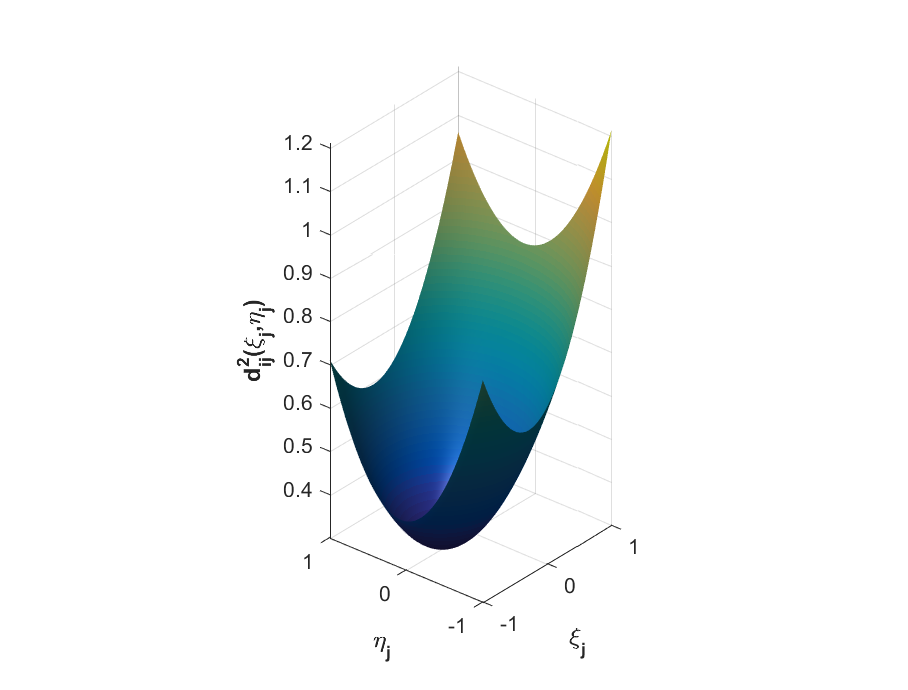
\includegraphics[width=0.5\textwidth]{images/Ch1/distance_squared.eps}
          } 
          \subfloat[Minimal distance configuration for a bi-linear quad element\label{fig.8b}]{%
            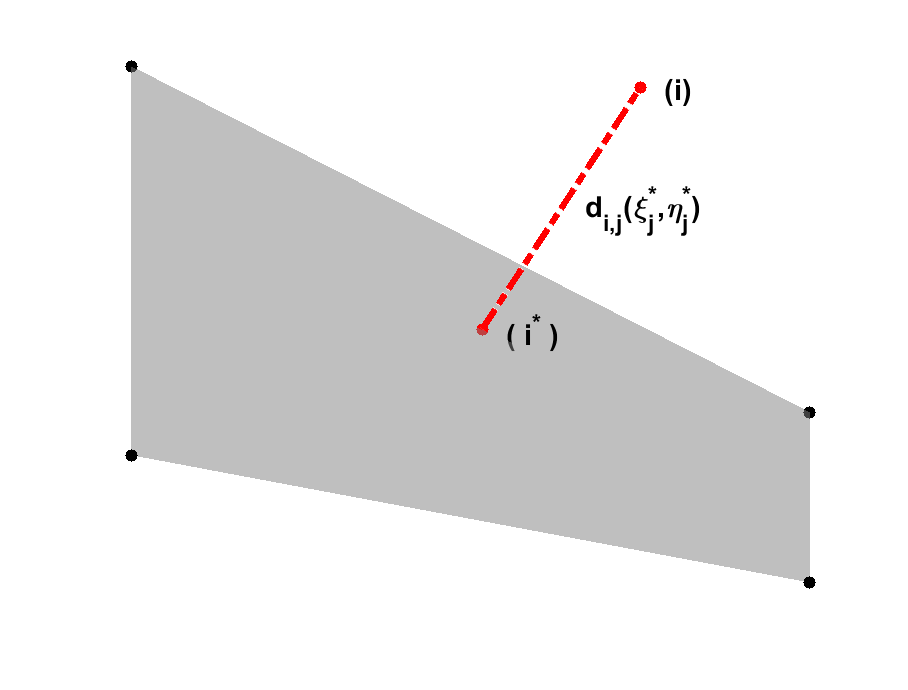
\includegraphics[width=0.5\textwidth]{images/Ch1/projection}
          }
          \caption{Node to element projection}
          \label{fig.8}
        \end{figure}
     When this procedure is used, for convex interface meshes there may be nodes that are far from the element $(j)$ but  that have their corresponding point $(i^*)$ inside the element $(j)$. The shape function of equation \eqref{eq.42} should take in account the minimal distance $d_{ij}\left(\xi^*_j,\eta^*_j \right)$: all the DOFs of the node $(i)$ at a distance superior to a given tolerance $t$ to its projection  $ (i^*) $ on $ \Gamma_j $ , should not be considered dependent on the $ (j) $ elements DOFs i.e.:
     \begin{equation}
     \label{eq.46}
     \Pi_{21i,j}=\begin{cases}\MatrixVar{N}_{j}^{\Gamma_1}\left(\xi^*,\eta^* \right) & d_{ij}\left(\xi^*_j,\eta^*_j \right)\leq t\\
     0 & \text{otherwise}.
     \end{cases}
     \end{equation}
\subsubsection{Weighted Residual Methods (WRM)}\label{sssec334}
The methods described until now are based on a strong formulation of the continuity on the interface of the displacement field (equation \eqref{eq.28}). On the other hand, segment to segment methods try to impose the continuity of displacements at the interface by the use of a weak form. One such method is the Weighted residual methods described in De Boer et al. \cite{de2007review}, Cebral{\=I} et al \cite{cebrali1997conservative} and  L{\"o}hner et al. \cite{lohner1998fluid} for the fluid-structure interaction problem.\footnote{These approaches do not make the use of Lagrange multipliers like in the Mortar methods (\cite{bernardi1989new},\cite{bernardi1993domain}); anyway when the shape functions of Lagrange multipliers are the same of the displacement field of the slave surface, the consequent equations are the same as it is also shown in Jeon et al. \cite{jeong2017element}} In this approach the jump of the displacement field across the interface has to be orthogonal in the $\mathbb{L}_2$ sense to the trace on $\Gamma_2$ of the kinematic admissible virtual displacement $\VectorVar{v} \in \mathbb{V}$:
\begin{equation}
\label{eq.47}
\begin{array}{cc}
  \int_{\Gamma}{\VectorVar{v}(\VectorVar{x})\cdot\left(\VectorVar{u}_{\Gamma_2}(\VectorVar{x})-\VectorVar{u}_{\Gamma_1}(\VectorVar{x}) \right)d\Gamma}=0 & \forall \VectorVar{v} \in \mathbb{V}    
\end{array}
\end{equation}
Discretizing $\VectorVar{v}(\VectorVar{x})$ using the shape functions of $\Gamma_2$  and using equation \eqref{eq.1.11} for each sub-domains and writing one equation for each shape function of the discretized space $\mathbb{V}^h_{\Gamma_2}$ equation \eqref{eq.47} becomes :
\begin{equation}
\label{eq.48}
\MatrixVar{M}_2\VectorVar{u}_{\Gamma_2}-\MatrixVar{M}_{21}\VectorVar{u}_{\Gamma_1}=\VectorVar{0}
\end{equation}
where the mass matrices are defined as:
\begin{eqnarray}
\label{eq.49}
M_{2i,j}=\int_{\Gamma}\MatrixVar{N}_{i}^{\Gamma_2}(\VectorVar{x})\cdot\MatrixVar{N}_{j}^{\Gamma_2}(\VectorVar{x})d\Gamma\\
\label{eq.50}
M_{21i,j}=\int_{\Gamma}\MatrixVar{N}_{i}^{\Gamma_2}(\VectorVar{x})\cdot\MatrixVar{N}_{j}^{\Gamma_1}(\VectorVar{x})d\Gamma
\end{eqnarray}
We can finally explicit the slave DOFs as a function of the master DOFs as:
\begin{equation}
\label{eq.51}
\VectorVar{u}_{\Gamma_2}=\MatrixVar{M}_2^{-1}\MatrixVar{M}_{21}\VectorVar{u}_{\Gamma_1}=\MatrixVar{\Pi}_{21}\VectorVar{u}_{\Gamma_1}
\end{equation}
It is shown in De Boer et al. \cite{de2007review}  that this method respects the condition of equation \eqref{eq32}, therefore the force resultant is conserved at the interface.
In order to evaluate the integral from equation \eqref{eq.49} and \eqref{eq.50} the support of the integral has to be chosen.

 \begin{figure}[!ht]
 \centering
     \subfloat[ Elements belonging to inconsistent meshes of the same  interface surface.\label{fig.9a}]{%
       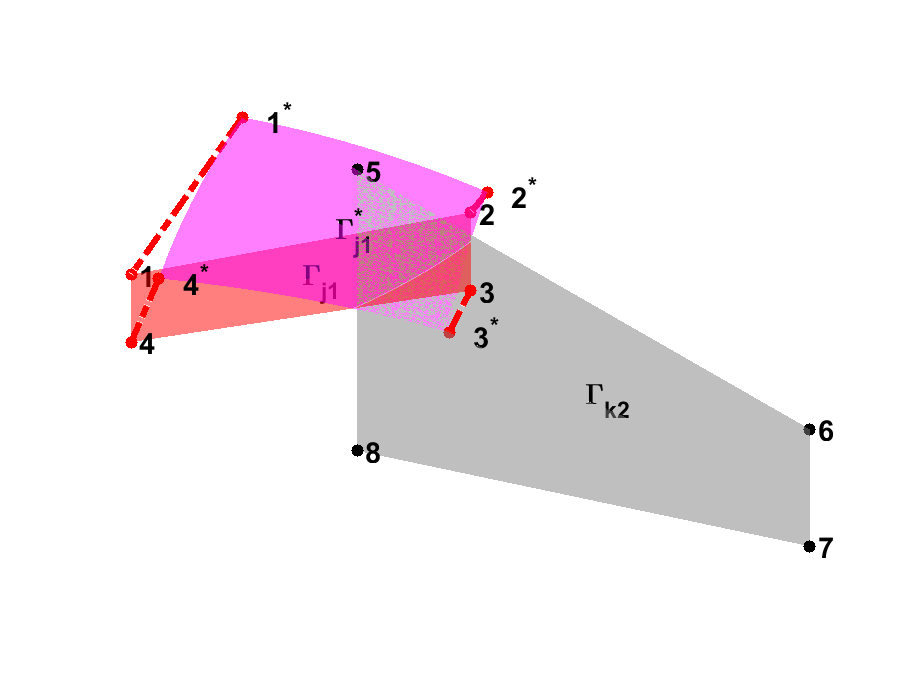
\includegraphics[width=0.6\textwidth]{images/Ch1/elementproj3}
     } \\
     \subfloat[ Projected master element on slave element  surface in slave local coordinates.\label{fig.9b}]{%
       \includegraphics[width=0.75\textwidth]{images/Ch1/projected_element}
     }
 
  
  \caption{Element to element projection examples. The master element surface $\Gamma_{j1}$ has been projected on the slave element surface $\Gamma_{k2}$ using the same procedure shown in figure (\ref{fig.8}) for each node of the element $j1$ ($1,2,3,4$). In this way it is possible to obtain the projected slave surface $\Gamma_{j1}^*$ ($1^*,2^*,3^*,4^*$). The union of the projection of all the elements of $\Gamma_1$ on $\Gamma_2$ is then indicated as $\Gamma_1^*$. After this projection, a change in local variables $(\xi_{k2},\eta_{k2})$ of the element $k2$ can be employed for the evaluation of Mass matrices (equations \eqref{eq.49} and \eqref{eq.50})}
  \label{fig.9}
\end{figure}
In fact in the most general case the surfaces described by the meshes will not be coincident and a projection will be needed (cf. figure (\ref{fig.9})) \footnote{Note that $\Gamma_{j1}^*$ sides are generally curved, in this work they are considered to be straight; this approximation will affect the accuracy of the evaluation of $ \mathbf{M_{21}}$ in equation \eqref{eq.50}. Nevertheless the error induced by this approximation can be considered negligible.}
\begin{figure}[!ht]
\centering
     \subfloat[ $N_{3^*}(\xi_{k2},\eta_{k2})$\label{fig.10a}]{%
       \includegraphics[width=0.3\textwidth]{images/Ch1/N3star}
     }
     \subfloat[  $N_{5}(\xi_{k2},\eta_{k2})$\label{fig.10b}]{%
       \includegraphics[width=0.3\textwidth]{images/Ch1/N5}
     }
     \subfloat[ $N_{3^*}(\xi_{k2},\eta_{k2})\cdot N_{5}(\xi_{k2},\eta_{k2})$\label{fig.10c}]{%
       \includegraphics[width=0.3\textwidth]{images/Ch1/N3sN5}
     }
     \caption{Shape function of node $3^*$ of $j1$, of node $5$ of $k2$ for the example of figure \ref{fig.9} and their product that has to be integrated in equation  \eqref{eq.50}, are represented.}
     \label{fig.10}
   \end{figure}
   \\
   One can observe that the integrand's support (cf. figure \ref{fig.10c}) is $\Gamma_{j1^*k2}\equiv \Gamma_{j1^*} \cap  \Gamma_{k2} $. The total support $\Gamma$ is therefore the union of all the intersections of each $\Gamma_{k2}$ with all corresponding projections $\Gamma_{j1^*}$ of $\Gamma_{j1}$ on $\Gamma_{k2}$:\\
\begin{equation}
\label{eq.52}
\Gamma\equiv\cup_{k2=1}^{N^{(e)}_2}\cup_{j1=1}^{N^{(e)}_1}\Gamma_{j1^*k2}
\end{equation}
 For the numeric evaluation of $\MatrixVar{M}_2$ and $\MatrixVar{M}_{21}$ we were inspired by the procedure in Puso et al. \cite{puso20043d}. Compared to Puso's original approach we implemented however some modifications in terms of node-to-element projection, and in terms of intersection polygon definition in order to render the procedure more robust. Instead of using the clipping algorithm of Foley \cite{foley1996computer} that may fail in some cases ( see \cite{gander2013algorithm} for further details), we implemented the procedure described by Gander et al. in \cite{gander2013algorithm}.
 To obtain the intersection polygon $\Gamma_{j1^*k2}$, firstly the nodes $(s1)$ of $\Gamma_{j1}$ that have a projection inside the element $(k2)$ are found.
Secondly the nodes $(s2)$ of $\Gamma_{k2}$ that are inside the projected element surface $\Gamma_{j1^*}$ are found.
Thirdly the intersection points $(s3)$ of all the sides of $\Gamma_{k2}$ with the one of $\Gamma_{j1^*}$ is carried out. The union of $(s1),(s2)$ and $(s3)$ form the vertices of the intersection polygon see figure \ref{fig.11a}.
\\
\begin{figure}[!ht]
     \subfloat[ Determination of $\Gamma_{j1^*k2}$ vertices. \label{fig.11a}]{%
       \includegraphics[width=0.5\textwidth]{images/Ch1/intersection_polygon}
     }
     \subfloat[  Integration over $\Gamma_{j1^*k2}$\label{fig.11b}]{%
       \includegraphics[width=0.5\textwidth]{images/Ch1/Gauss_point.eps}
     }
     \caption{Procedure for the determination of  $\Gamma_{j1^*k2}$ vertices and consequent numerical integration }
     \label{fig.11}
   \end{figure}
A triangulation of this polygon is obtained connecting all the sides with the polygon center. Finally, 3 Gauss points per triangle have to be used for the numerical integration of equation \eqref{eq.49} and \eqref{eq.50}) (see the example of figure \ref{fig.11b}). The Gauss point local coordinates  $(\VectorVar{\Xi}_{k2}^{(GP)},\VectorVar{\Theta}_{k2}^{(GP)})$ are easy to find as a function of the triangulation coordinates. On the other hand, to know the value of $\MatrixVar{N}_{j}^{\Gamma_1}$ on the corresponding points of $\Gamma_{j1^*}$ for equation \eqref{eq.50}), the local coordinates  $(\VectorVar{\Xi}_{j1}^{(GP)},\VectorVar{\Theta}_{j1}^{(GP)})$  have to be determined. Puso suggested even for this projection to use the normal of element ($k2$) on the center of the element. To be completely rigorous one should evaluate the normal to the surface $\Gamma_{k2}$ in each Gauss point and then make an intersection of the line on which the normal lies and the surface of $\Gamma_{j1}$ to finally have the local coordinates $(\VectorVar{\Xi}_{j1}^{(GP)},\VectorVar{\Theta}_{j1}^{(GP)})$ . In other words we should find the roots of the nonlinear system of equations:
\begin{multline}
\label{eq.53}
2\nabla\VectorVar{x}_{\Gamma_{k2}}\left(\VectorVar{\Xi}_{k2}^{(GP)},\VectorVar{\Theta}_{k2}^{(GP)}\right)\cdot \\ \cdot\left( \VectorVar{x}_{\Gamma_{k2}}\left(\VectorVar{\Xi}_{k2}^{(GP)},\VectorVar{\Theta}_{k2}^{(GP)}\right)-\VectorVar{x}_{\Gamma_{j1}}\left(\VectorVar{\Xi}_{j1}^{(GP)},\VectorVar{\Theta}_{j1}^{(GP)}\right)\right)= \VectorVar{0}
\end{multline}
Taking in consideration the fact that the sides of $\Gamma_{j1^*}$ are considered as straight segment between the projection on  $\Gamma_{k2}$ of the nodes of $(j1)$, even if this is not always the case, the use of equation \eqref{eq.53} is not recommended. Some Gauss points when re-projected on $\Gamma_{j1}$ could lie outside the element $(j1)$. To avoid this situation a geometric isoparametric interpolation between the local coordinate $(\xi_{j1},\eta_{j1})$ and the projected one $(\xi_{k2},\eta_{k2})$ is considered here:
\begin{eqnarray}
\label{eq.54}
\begin{aligned}
\xi_{k2}\left(\xi_{j1},\eta_{j1}\right)=\xi_{k2}^{1^*}N_1\left( \xi_{j1},\eta_{j1}\right)+\xi_{k2}^{2^*}N_2\left( \xi_{j1},\eta_{j1}\right)+\xi_{k2}^{3^*}N_3\left( \xi_{j1},\eta_{j1}\right)+\xi_{k2}^{4^*}N_4\left( \xi_{j1},\eta_{j1}\right)
\end{aligned} \\
\label{eq.55}
\begin{aligned}
\eta_{k2}\left(\xi_{j1},\eta_{j1}\right)=\eta_{k2}^{1^*}N_1\left( \xi_{j1},\eta_{j1}\right)+\eta_{k2}^{2^*}N_2\left( \xi_{j1},\eta_{j1}\right)+\eta_{k2}^{3^*}N_3\left( \xi_{j1},\eta_{j1}\right)+\eta_{k2}^{4^*}N_4\left( \xi_{j1},\eta_{j1}\right) 
\end{aligned} 
\end{eqnarray}
Where $(\xi_{k2}^{n^*},\xi_{k2}^{n^*})$ are the local coordinates of the projection of the n-th node of $(j1)$ on $\Gamma_{k2}$ and $N_n$ are the classic bilinear shape functions:
\begin{equation}
\begin{array}{cc}
\label{eq.56}
N_1\left( \xi_{j1},\eta_{j1}\right)=\frac{1}{4}\left( 1-\xi_{j1}\right)\left( 1-\eta_{j1}\right) \\ N_2\left( \xi_{j1},\eta_{j1}\right)=\frac{1}{4}\left( 1-\xi_{j1}\right)\left( 1+\eta_{j1}\right) \\
N_3\left( \xi_{j1},\eta_{j1}\right)=\frac{1}{4}\left( 1+\xi_{j1}\right)\left( 1+\eta_{j1}\right) \\ N_4\left( \xi_{j1},\eta_{j1}\right)=\frac{1}{4}\left( 1+\xi_{j1}\right)\left( 1-\eta_{j1}\right)
\end{array}
\end{equation}
Finally, equation \eqref{eq.54}-\eqref{eq.55} can be used to find $(\VectorVar{\Xi}_{j1}^{(GP)},\VectorVar{\Theta}_{j1}^{(GP)})$ solving another nonlinear system of equations:
\begin{eqnarray}
\label{eq.57}
\VectorVar{\Xi}_{k2}^{(GP)}-\xi_{k2}\left( \VectorVar{\Xi}_{j1}^{(GP)},\VectorVar{\Theta}_{j1}^{(GP)}\right)=\VectorVar{0} \\
\label{eq.58}
\VectorVar{\Theta}_{k2}^{(GP)}-\eta_{k2}\left( \VectorVar{\Xi}_{j1}^{(GP)},\VectorVar{\Theta}_{j1}^{(GP)}\right)=\VectorVar{0} 
\end{eqnarray}
This system can be solved numerically (e.g. with a Newton-Raphson algorithm) giving the analytical expression of the Jacobian matrix. In figure \ref{fig.12} the Gauss points are projected from $\Gamma_{j1*k2}$ back on $\Gamma_{j1}$ using the iso-parametric projection of equations \eqref{eq.57}-\eqref{eq.58}.
\begin{figure}[ht]
\centering
\includegraphics[width=8cm]{images/Ch1/PGproj}
\caption{Gauss point projection from $\Gamma_{j1*k2}$ back on $\Gamma_{j1}$ using the iso-parametric projection of equations \eqref{eq.57}-\eqref{eq.58}.}  
\label{fig.12}
\end{figure}
\subsection{Variational based approaches}\label{ssec34}
In variational approaches, instead of using the principle of virtual work to get the final system of equations, the displacement field solution of the static problem will be sought to minimize the total energy:
\begin{equation}
\label{eq.59}
E(\VectorVar{u})=\VectorVar{u}^T\MatrixVar{K}\VectorVar{u}-\VectorVar{u}^T\VectorVar{f}
\end{equation}
Considering the partition that we already introduced, the total energy becomes:
\begin{equation}
\label{eq.60}
\begin{aligned}
E( \VectorVar{u}_1,\VectorVar{u}_{\Gamma_1},\VectorVar{u}_{\Gamma_2},\VectorVar{u}_2
    )=\left\lbrace\begin{array}{cccc} \VectorVar{u}_1^T&\VectorVar{u}_{\Gamma_1}^T&\VectorVar{u}_{\Gamma_2}^T&\VectorVar{u}_2^T
    \end{array}\right\rbrace \\\left(\left[ \begin{array}{cccc} 
    \MatrixVar{K}_{1,1} & \MatrixVar{K}_{1,\Gamma_1} & \MatrixVar{0}& \MatrixVar{0} \\
   \MatrixVar{K}_{\Gamma_1,1} & \MatrixVar{K}_{\Gamma_1,\Gamma_1} & \MatrixVar{0}& \MatrixVar{0}\\ \MatrixVar{0}& \MatrixVar{0}& \MatrixVar{K}_{\Gamma_2,\Gamma_2}&\MatrixVar{K}_{\Gamma_2,2}\\   
    \MatrixVar{0} & \MatrixVar{0}& \MatrixVar{K}_{2,\Gamma_2} & \MatrixVar{K}_{2,2}\end{array} \right]\left\lbrace\begin{array}{c} \VectorVar{u}_1\\\VectorVar{u}_{\Gamma_1}\\\VectorVar{u}_{\Gamma_2}\\\VectorVar{u}_2
    \end{array}\right\rbrace
    -\left\lbrace\begin{array}{c} \VectorVar{f}_1\\\VectorVar{f}_{\Gamma_1}\\\VectorVar{f}_{\Gamma_2}\\\VectorVar{f}_2
    \end{array}\right\rbrace\right)
\end{aligned}
\end{equation}
Note that in equation \eqref{eq.60} the work at the interface of the residual is eliminated for energy conservation. The system of equations that comes from this formulation has a singular matrix, so that the solution of the static problem cannot be simply obtained by minimizing the total energy.
\subsubsection{Mortar Element Method}\label{sssec341}
The basic idea of the Mortar approach is to add a dislocation potential to the total energy, in order to impose the continuity of the displacement field at the interface:
\begin{equation}
\label{eq.61}
E_d\left( \VectorVar{u}, \VectorVar{\lambda} \right)=\int_{\Gamma} \VectorVar{\lambda}\left(\VectorVar{u}|_{\Gamma_1}-\VectorVar{u}|_{\Gamma_2}\right)d\Gamma
\end{equation}
This potential is summed with the total energy to get the Lagrangian functional $E_l \left(\VectorVar{u}, \VectorVar{\lambda} \right)=E_d\left( \VectorVar{u}, \VectorVar{\lambda} \right)+E(\VectorVar{u})$ whose stationary points are the solution of the constrained optimization:
\begin{equation}
\label{eq.62}
\left\lbrace \begin{array}{c}
\min_{\VectorVar{u}}(E(\VectorVar{u}))\\
  \VectorVar{u}|_{\Gamma_1}-\VectorVar{u}|_{\Gamma_2}=0
\end{array}\right.
\end{equation}
Similarly to Master/Slave approaches, the mortar approach needs the choice of one surface to be the mortar surface and the other to be the non-mortar.
The interpolation functions of the Lagrangian multipliers $\VectorVar{\lambda}$ are (in the case of two domains) chosen to be the same as those of the slave surface:\footnote{In the work of Puso et al \cite{puso20043d} the dual space is also employed}
\begin{equation}
\label{eq.63}
\VectorVar{\lambda}(\VectorVar{x}|_{\Gamma_2})=\MatrixVar{N}(\VectorVar{x}|_{\Gamma_2})\VectorVar{\lambda}_{\Gamma_2}
\end{equation}
The dislocation potential can then be written as:
\begin{equation}
\label{eq.64}
E_d( \VectorVar{u}_{\Gamma_1},\VectorVar{u}_{\Gamma_2},\VectorVar{\lambda}_{\Gamma_2})=\VectorVar{\lambda}_{\Gamma_2}^T\left(\MatrixVar{M}_{21}\VectorVar{u}_{\Gamma_1}-\MatrixVar{M}_2\VectorVar{u}_{\Gamma_2}\right)
\end{equation}
Then the Lagrangian functional is stationary  for:
\begin{equation}
\label{eq.65}
 \left[ \begin{array}{ccccc} 
    \MatrixVar{\mathbf{K}}_{1,1} & \MatrixVar{\mathbf{K}}_{1,\Gamma_1} &\MatrixVar{0} &\MatrixVar{0}& \MatrixVar{0} \\
   \MatrixVar{\mathbf{K}}_{\Gamma_1,1} & \MatrixVar{\mathbf{K}}_{\Gamma_1,\Gamma_1} &\MatrixVar{M}_{21}^T & \MatrixVar{0}& \MatrixVar{0}\\ \MatrixVar{0} &\MatrixVar{M}_{21} &\MatrixVar{0} &-\MatrixVar{M}_{2}& \MatrixVar{0}\\\MatrixVar{0}& \MatrixVar{0}& -\MatrixVar{M}_{2}^T & \MatrixVar{\mathbf{K}}_{\Gamma_2,\Gamma_2} &\MatrixVar{\mathbf{K}}_{\Gamma_2,2}\\   
    \MatrixVar{0} & \MatrixVar{0}&\MatrixVar{0}& \MatrixVar{\mathbf{K}}_{2,\Gamma_2} & \MatrixVar{\mathbf{K}}_{2,2}\end{array} \right]\left\lbrace\begin{array}{c} \VectorVar{u}_1\\\VectorVar{u}_{\Gamma_1}\\\VectorVar{\lambda}_{\Gamma_2}\\\VectorVar{u}_{\Gamma_2}\\\VectorVar{u}_2
    \end{array}\right\rbrace=\left\lbrace\begin{array}{c} \VectorVar{f}_1\\\VectorVar{f}_{\Gamma_1}\\\VectorVar{0}\\\VectorVar{f}_{\Gamma_2}\\\VectorVar{f}_2
    \end{array}\right\rbrace
\end{equation}
Even if the equations obtained from this approach seem to be different from the one of the WRM, eliminating the Lagrange eigenvalues from equation \eqref{eq.65} we can recognize that they have the same solution (see Jeong et al. \cite{jeong2017element} for the proof). It can be noted that this method has the same difficulties of implementation and of evaluation cost encountered with the WRM method: The integral of the shape function over the intersection of the interface has to be evaluated in order to evaluate the mass matrices $\MatrixVar{M}_{21},\MatrixVar{M}_{2}$. The Mortar approach is shown to be as accurate as the WRM approach but with a noticeably longer effort due to the increased number of variables. For this reason in section \ref{sec4} only WRM has been implemented and compared with other methods.
\subsection{The Internodes Approach}\label{ssec35}
Here we describe the internodes approach, introduced by Deparis et al in \cite{deparis2016internodes} and further analyzed by Gervasio et al. in \cite{gervasio2016analysis}. We derived its matrix formulation directly from equation \eqref{eq.15}. Like in the elimination approaches the continuity of the displacement field is guaranteed by equation \eqref{eq.28}. On the other hand the balance of energy and force sum are not imposed. The forces $\VectorVar{t}_{12}$ and $\VectorVar{t}_{21}$ are supposed to be interpolated with the same shape functions of displacement  on each subdomain interface:
\begin{eqnarray}
\label{eq.66}
 \VectorVar{t}_{12}(\VectorVar{x}|_{\Gamma_2})=\MatrixVar{N}^{(h)}(\VectorVar{x}|_{\Gamma_2}) \VectorVar{p}_{2}\\
 \label{eq.67}
 \VectorVar{t}_{21}(\VectorVar{x}|_{\Gamma_1})=\MatrixVar{N}^{(h)}(\VectorVar{x}|_{\Gamma_1}) \VectorVar{p}_{1}
\end{eqnarray}
where $\VectorVar{p}_{1}$ and $\VectorVar{p}_{2}$ are the vector of internal forces per unit of surface interpolating $\VectorVar{t}_{12}(\VectorVar{x}|_{\Gamma_2})$ and $ \VectorVar{t}_{21}(\VectorVar{x}|_{\Gamma_1})$.
Conforming to these definitions the residual at the interface may be evaluated as:
\begin{eqnarray}
\label{eq.68}
 \VectorVar{r}_{\Gamma_1}=\int_{\Gamma_1}\MatrixVar{N}^{(h)}(\VectorVar{x}|_{\Gamma_1})\cdot\MatrixVar{N}^{(h)}(\VectorVar{x}|_{\Gamma_1}) \VectorVar{p}_{1}d\Gamma_1=\MatrixVar{M}_1\VectorVar{p}_{1}\\
 \label{eq.69}
\VectorVar{r}_{\Gamma_2}=\int_{\Gamma_2}\MatrixVar{N}^{(h)}(\VectorVar{x}|_{\Gamma_2})\cdot\MatrixVar{N}^{(h)}(\VectorVar{x}|_{\Gamma_2}) \VectorVar{p}_{2}d\Gamma_2=\MatrixVar{M}_2\VectorVar{p}_{2}
\end{eqnarray}
The balance of the internal forces per unit area is imposed in a similar fashion to the continuity of the displacements as in equation \eqref{eq.28}, but this time a second interpolation operator is used:
\begin{equation}
\label{eq.70}
\VectorVar{p}_{1}+\MatrixVar{\Pi}_{12}\VectorVar{p}_{2}=\VectorVar{0}
\end{equation}
Substituting equation \eqref{eq.68} and \eqref{eq.69} in \eqref{eq.70} one gets:
\begin{equation}
\label{eq.71}
\VectorVar{r}_{\Gamma_1}+\MatrixVar{M}_1\MatrixVar{\Pi}_{12}\MatrixVar{M}_2^{-1}\VectorVar{r}_{\Gamma_2}=\VectorVar{r}_{\Gamma_1}+\MatrixVar{Q}_{12}\VectorVar{r}_{\Gamma_2}=\VectorVar{0}
\end{equation}
Finally, using equations \eqref{eq.71} and \eqref{eq.28} in \eqref{eq.15} one can get:
\begin{equation}
\label{eq.72}
\begin{aligned}
\left[ \begin{array}{ccc} 
    \MatrixVar{\mathbf{K}}_{1,1} & \MatrixVar{\mathbf{K}}_{1,\Gamma_1} & \MatrixVar{0} \\
   \MatrixVar{\mathbf{K}}_{\Gamma_1,1} & \MatrixVar{\mathbf{K}}_{\Gamma_1,\Gamma_1}+ \MatrixVar{Q}_{12}\MatrixVar{\mathbf{K}}_{\Gamma_2,\Gamma_2}\MatrixVar{\Pi}_{21} & \MatrixVar{Q}_{12}\MatrixVar{\mathbf{K}}_{\Gamma_2,2}\\   
    \MatrixVar{0} & \MatrixVar{\mathbf{K}}_{2,\Gamma_2}\MatrixVar{\Pi}_{21} & \MatrixVar{\mathbf{K}}_{2,2}\end{array} \right] \left\lbrace \begin{array}{c} \VectorVar{u}_1\\\VectorVar{u}_{\Gamma_1}\\\VectorVar{u}_2
    \end{array}\right\rbrace= \left\lbrace\begin{array}{c} \VectorVar{f}_1\\\VectorVar{f}_{\Gamma_1}+\MatrixVar{Q}_{12}\VectorVar{f}_{\Gamma_2}\\\VectorVar{f}_2
    \end{array}\right\rbrace
    \end{aligned}
\end{equation}
It can be observed that the system of equations of the internodes formulation is not symmetric and that equations \eqref{eq.31} and \eqref{eq32} are not imposed, so that internodes does not conserve \textit{apriori} neither work nor resultants of forces and moments. On the other hand the formulation and the implementation are straightforward if compared with the mortar and the WRM approaches: only the mass matrices $\MatrixVar{M}_2$, $\MatrixVar{M}_1$ and the interpolation operators $\MatrixVar{\Pi}_{12}$ and $\MatrixVar{\Pi}_{21}$ are needed. Good convergence properties have been showed in the work of Gervasio et al. \cite{gervasio2016analysis}.
\subsection{Weighted Average Continuity Approach (WACA)}\label{sssec36}
The collocation approaches even if simple are not accurate enough when the most refined mesh is chosen as master surface. On the other hand the segment to segment approaches are very accurate but are complex and need much more computational effort. The Internodes approach seeks to achieve such a trade-off between complexity and accuracy but, as it will be shown in section \ref{sec4}, the fact that it does not conserve the resultant force vector and total energy at the interface can deteriorate its accuracy. In \cite{coniglio2018weighted} we proposed a new approach that shares with Internodes its simplicity but achieves an improved accuracy.
This one is based on another expression of the continuity of the displacement field at the interface. Before we introduce the new formulation let us highlight some equations that can be derived. Each line of the vector coming from the multiplication of the interface mass matrix and the interface displacement vector represents the integral over the interface of the displacement field times the shape function of the DOF corresponding to the selected line. We can define a weighted average displacement field using as weight the shape function:
\begin{equation}
\label{eq.73a}
\bar{u}_{\Gamma_1i}=\frac{\int_{\Gamma_1}\VectorVar{u}(\VectorVar{x}\|_{\Gamma_1})\cdot\MatrixVar{N}_{i}^{\Gamma_1}(\VectorVar{x}\|_{\Gamma_1})d\Gamma_1}{\int_{\Gamma_1(\MatrixVar{N}_{i}^{\Gamma_1}(\VectorVar{x}\|_{\Gamma_1}))_id\Gamma_1}}
\end{equation}
this can be reformulated as:
\begin{equation}
\label{eq.73}
({M}_{1}{u}_{\Gamma_1})_i=S_{N_i}\bar{u}_{\Gamma_1i}
\end{equation}
where $S_{N_i}$ is the integral of the i-th shape function over its support  and $\bar{u}_{\Gamma_1i}$ is the weighted average of the i-th displacement on $\Gamma_1$. 
We can put this relationship in the matrix form:
\begin{eqnarray}
\label{eq.74}
\MatrixVar{M}_{1}\VectorVar{u}_{\Gamma_1}=\MatrixVar{S}_1\VectorVar{\bar{u}}_{\Gamma_1}\qquad
\MatrixVar{M}_{2}\VectorVar{u}_{\Gamma_2}=\MatrixVar{S}_2\VectorVar{\bar{u}}_{\Gamma_2}
\end{eqnarray}
where we denote with $\MatrixVar{S}_1$ and $\MatrixVar{S}_2$ the diagonal matrices containing on the diagonal the integral of each shape function on its support\footnote{$\MatrixVar{S}_1$ and $\MatrixVar{S}_2$ are also denoted as lumped mass matrices}, and with $\VectorVar{\bar{u}}_{\Gamma_1}$ and $\VectorVar{\bar{u}}_{\Gamma_2}$ the weighted average displacement field of each component over the corresponding shape function support.
In the approach we propose we seek to state the continuity of the weighted average displacement interpolating between the two surfaces i.e.
\begin{equation}
\label{eq.75}
\VectorVar{\bar{u}}_{\Gamma_2}=\MatrixVar{\Pi}_{21}\VectorVar{\bar{u}}_{\Gamma_1}
\end{equation}
By substitution of equation \eqref{eq.74}  into equation  \eqref{eq.75} one gets a new interpolation operator between the displacement fields:
\begin{equation}
\label{eq.76}
\VectorVar{u}_{\Gamma_2}=\MatrixVar{M}_{2}^{-1}\MatrixVar{S}_2\MatrixVar{\Pi}_{21}\MatrixVar{S}_1^{-1}\MatrixVar{M}_{1}\VectorVar{u}_{\Gamma_1}=\MatrixVar{\Pi}_{21}^{*}\VectorVar{u}_{\Gamma_1}
\end{equation}
If the interpolation operator $\MatrixVar{\Pi}_{21}$ satisfies the conservation conditions given by equation \eqref{eq32}, $\MatrixVar{\Pi}^{*}_{21}$ will also satisfy the same conditions:
\begin{equation}
\label{eq.77}
\begin{aligned}
\MatrixVar{\Pi}_{21}^{*}\MatrixVar{1}_{\Gamma_1}=\MatrixVar{M}_{2}^{-1}\MatrixVar{S}_2\MatrixVar{\Pi}_{21}\MatrixVar{S}_1^{-1}\MatrixVar{M}_{1}\MatrixVar{1}_{\Gamma_1}=\MatrixVar{M}_{2}^{-1}\MatrixVar{S}_2\MatrixVar{\Pi}_{21}\MatrixVar{S}_1^{-1}\MatrixVar{S}_1\MatrixVar{1}_{\Gamma_1}=\\=
\MatrixVar{M}_{2}^{-1}\MatrixVar{S}_2\MatrixVar{\Pi}_{21}\MatrixVar{1}_{\Gamma_1}=\MatrixVar{M}_{2}^{-1}\MatrixVar{S}_2\MatrixVar{1}_{\Gamma_2}=\MatrixVar{M}_{2}^{-1}\MatrixVar{M}_{2}\MatrixVar{1}_{\Gamma_2}=\MatrixVar{1}_{\Gamma_2}
\end{aligned}
\end{equation}
where we used twice the fact that the mass coherent and lumped mass matrices conserve the sum of lines i.e.
\begin{eqnarray}
\label{eq.78}
\MatrixVar{M}_{1}\MatrixVar{1}_{\Gamma_1}=\MatrixVar{S}_{1}\MatrixVar{1}_{\Gamma_1} \qquad \MatrixVar{M}_{2}\MatrixVar{1}_{\Gamma_2}=\MatrixVar{S}_{2}\MatrixVar{1}_{\Gamma_2} 
\end{eqnarray}
The condition of zero work at the interface (equation \eqref{eq.29}) can be used as was done in the classic elimination methods so that the final matrix form of the WACA approach is:
\begin{equation}
\label{eq.79}
\begin{aligned}
\left[ \begin{array}{ccc} 
    \MatrixVar{\mathbf{K}}_{1,1} & \MatrixVar{\mathbf{K}}_{1,\Gamma_1} & \MatrixVar{0} \\
   \MatrixVar{\mathbf{K}}_{\Gamma_1,1} & \MatrixVar{\mathbf{K}}_{\Gamma_1,\Gamma_1}+ (\MatrixVar{\Pi}_{21}^{*})^T\MatrixVar{\mathbf{K}}_{\Gamma_2,\Gamma_2}\MatrixVar{\Pi}_{21}^* & (\MatrixVar{\Pi}_{21}^{*})^T\MatrixVar{\mathbf{K}}_{\Gamma_2,2}\\   
    \MatrixVar{0} & \MatrixVar{\mathbf{K}}_{2,\Gamma_2}\MatrixVar{\Pi}^{*}_{21} & \MatrixVar{\mathbf{K}}_{2,2}\end{array} \right] \left\lbrace \begin{array}{c} \VectorVar{u}_1\\\VectorVar{u}_{\Gamma_1}\\\VectorVar{u}_2
    \end{array}\right\rbrace=\\ \left\lbrace\begin{array}{c} \VectorVar{f}_1\\\VectorVar{f}_{\Gamma_1}+(\MatrixVar{\Pi}_{21}^{*})^T\VectorVar{f}_{\Gamma_2}\\\VectorVar{f}_2
    \end{array}\right\rbrace
\end{aligned}
\end{equation}
This formulation shares the same simplicity of the Internodes approach, on the other hand satisfies \textit{\textit{a priori}} the conservation of the residual sum at the interface and of the energy at the interface.  

\subsection{\textit{A priori} conservation of moments}\label{ssec37}
All the methods proposed here do respect the balance of residual resultant and residual work but do not respect an \textit{a priori} condition on the moments of the resultant at the interface. In the work of Puso \cite{puso20043d}, to enforce this balance of moments and keep the same formulation of the mortar method the nodes of the slave surface in the undeformed configuration are moved on the interface surface. This method is interesting but still not very practical to conserve the meshes of both sub-domains. Another interesting approach is proposed by  Park et al. in \cite{park2002simpl}, were a third surface and mesh (the frame) are introduced and the balance of moments and of the patch test are satisfied choosing the position of nodes on the frame. To the authors' best knowledge no works exist which propose to satisfy the moments' balance equation through an \textit{a priori} condition on the interpolation operators $\Pi_{12}$, $\Pi_{21}$. This is the objective of this subsection in which a necessary condition is determined and used to correct the projection operator for all eliminations methods as well as for the new WACA method.
First of all let’s write the balance of moments of the residual:
\begin{equation}
\label{eq.80}
\sum_{i=1}^{n_{\Gamma_1}}\VectorVar{OP}_{i\Gamma_1}\times \VectorVar{R}_{i\Gamma_1}+\sum_{j=1}^{n_{\Gamma_2}}\VectorVar{OP}_{j\Gamma_2}\times \VectorVar{R}_{j\Gamma_2}=\VectorVar{0}
\end{equation}
We defined here $\VectorVar{OP}_{i\Gamma_s}$ as the vector connecting the fixed point O to the positions of the $i^{th}$ nodes of the $\Gamma_s$ surface (s=1,2); $\VectorVar{R}_{i\Gamma_s}$ as the vector of the residual force at the same node. This equation must be satisfied for each possible combination of residuals. For the energy balance \eqref{eq.31} the residuals are not independent so that all the combinations of residuals can be obtained as all the vectors in $\VectorVar{R}^{N_{\Gamma_2}}$ where $N_{\Gamma_2}=n_d n_{\Gamma_2}$ is the number of DOFs of the second interface. Satisfying equation \eqref{eq.80} for all vectors of $\VectorVar{R}^{N_{\Gamma_2}}$ means that it has to be verified for each vector in a normal basis, for example the canonical one.
For each node $j$ and for each direction $n_d^{(j)}$ (for each $k_2$ DOF) we can then write 3 equations as follows: 
\begin{eqnarray}
\label{eq.80b}
\begin{aligned}
\sum_{i=1}^{n_{\Gamma_1}}\VectorVar{OP}_{i\Gamma_1}\times (\VectorVar{R}_{i\Gamma_1})_{n_d^{(i)}}+\VectorVar{OP}_{j\Gamma_2}\times (\VectorVar{R}_{j\Gamma_2})_{n_d^{(j)}}=\VectorVar{0} \quad \forall k_2\in \lbrace1,2,\dots,N_{\Gamma_2} \rbrace
\end{aligned}
\end{eqnarray}
By the use of \eqref{eq.31} on can replace $(\VectorVar{R}_{i\Gamma_1})_{n_d^{(i)}}$ by the $(k_2,\VectorVar{k_1})$ terms of $\MatrixVar{\Pi}_{21}$ , that we will denote here as $\left(\VectorVar{\Pi_{21}}\right)_{(k_2,\VectorVar{k_1})}$, where   $\VectorVar{k_1}$ are the indexes of the DOFs of the $i^{th}$ node of $\Gamma_1$. Choosing $O \equiv P_{j\Gamma_2} $ to write each moment equation, equation \eqref{eq.80b} becomes:
\begin{eqnarray}
\label{eq.80c}
\begin{aligned}
\sum_{i=1}^{n_{\Gamma_1}}\VectorVar{P_{j\Gamma_2}P_{i\Gamma_1}}\times \left(\VectorVar{\Pi_{21}}\right)_{(k_2,\VectorVar{k_1})}^T=\VectorVar{0} \quad \forall k_2\in \lbrace1,2,\dots,N_{\Gamma_2} \rbrace
\end{aligned}
\end{eqnarray}
This equation can be also written in the following matrix form:
\begin{eqnarray}
\label{eq.80d}
\left(\VectorVar{\Pi_{21}}\right)_{k_2}\cdot\MatrixVar{B}_{k2}=\VectorVar{0} \qquad \forall k_2\in \lbrace1,2,\dots,N_{\Gamma_2} \rbrace
\end{eqnarray}
Where $\left(\VectorVar{\Pi_{21}}\right)_{k_2}$ is the $k_2^{th}$ line of $\MatrixVar{\Pi}_{21}$, $\MatrixVar{B}_{k2}$ is a matrix $N_{\Gamma_1}\times3$ defined by:
\begin{eqnarray}
\label{eq.80e}
(\MatrixVar{B}_{k2})_{(k_1,n_d)}=(\VectorVar{P_{j\Gamma_2}P_{i\Gamma_1}}\times\VectorVar{n_d}^{(k_1)})_{n_d}
\end{eqnarray}
 $\VectorVar{n_d}^{(k_1)}$ is the $3\times1$ versor of the $k_1^{th}$ DOF direction and by $(\bullet)_{n_d}$ the extraction of the  ${n_d}$ component of a vector. Equation \eqref{eq.80d} and equation \eqref{eq32} form a system of 6 equations for each line of the projecting operator that can be compactly written as:
 \begin{equation}
 \label{eq.80f}
 \left(\VectorVar{\Pi_{21}}\right)_{k_2}\cdot\MatrixVar{A}_{k_2}^T=\left(\VectorVar{\Pi_{21}}\right)_{k_2}\cdot\left[
 \begin{array}{c c}
   \MatrixVar{1}_{\Gamma_1}&
   \MatrixVar{B}_{k2}
 \end{array}
 \right]=\left[\begin{array}{c c}
   \left(\VectorVar{1_{\Gamma_2}}\right)_{k_2}&
   \VectorVar{0}
 \end{array}
 \right]=\VectorVar{b}^T
 \end{equation}
 We seek to correct the projection operator coming from an elimination approach (RBF, WRM, WACA) to respect equation \eqref{eq.80f}. Since we do not want to significantly modify the previous interpolations, we would like to have a new line  $ \left(\VectorVar{\Pi_{21}}\right)_{k_2}^{(c)}$ that is as close as possible to the original one  $ \left(\VectorVar{\Pi_{21}}\right)_{k_2}$ and that satisfies equation \eqref{eq.80f}. In other terms we want to solve the optimization problem
 \begin{equation}
 \label{eq.80g}
\left\lbrace \begin{array}{c}
 min_{\VectorVar{s}}\left(\VectorVar{s}-\left(\VectorVar{\Pi_{21}}\right)_{k_2} \right)^T\cdot\left(\VectorVar{s}-\left(\VectorVar{\Pi_{21}}\right)_{k_2} \right)\\
 \VectorVar{s}\cdot\MatrixVar{A}_{k_2}^T=\VectorVar{b}^T
 \end{array} \right.
 \end{equation}
 Here we indicated $ \left(\VectorVar{\Pi_{21}}\right)_{k_2}^{(c)}$ as $\VectorVar{s}$ for brevity. To solve this constrained optimization problem the Lagrangian approach can be used. The stationary condition of the Lagrangian form a linear system of equations that can be solved to find  $\VectorVar{s}^T$ is:
 \begin{equation}
 \label{eq.80h}
\left(\left(\VectorVar{\Pi_{21}}\right)_{k_2}^{(c)}\right)^T=\left(\VectorVar{\Pi_{21}}\right)_{k_2}^T+\MatrixVar{A}_{k_2}^T\cdot(\MatrixVar{A}_{k_2}\cdot\MatrixVar{A}_{k_2}^T)^{-1}(\VectorVar{b}-\MatrixVar{A}_{k_2}\cdot\left(\VectorVar{\Pi_{21}}\right)_{k_2}^T)
 \end{equation}
 The resulting operator $\MatrixVar{\Pi}_{21}^{(c)}$ will then respect both the balance of resultant of residual/energy and moments. Still, its precision in terms of displacement and stress continuity could be affected, so in the next section we will analyze its numerical efficiency. The correction presented here can be adapted even for the Internodes approach. The corrected scheme will modify the column of the $\MatrixVar{Q}_{12}$ and not the line of $\MatrixVar{\Pi}_{21}$. The resulting scheme will therefore conserve the balance  of forces and moments but not of energy since $\MatrixVar{Q}_{12}^{(c)}\neq\MatrixVar{\Pi}_{21}^T$.
 \subsection{Benchmarking on numerical test cases}\label{sec4}
 \subsubsection{Test cases definition and analysis for consistent meshes}\label{ssec41}
 In this section we present two test case geometries, each investigated under pure traction and bending-traction boundary conditions, which will serve for benchmarking various methods considered. The first case is a column like structure with spherical ends see figure \ref{fig.13a}. In the second case (figure \ref{fig.13b}) the bottom structure is wider and shorter than the upper one and both ends are spherical. Both structures are completely fixed at the bottom face and for the pure traction loading they are loaded on the upper surface with a constant surface traction in the z direction of magnitude 30.25 MPa. The analysis made for configuration (1) is actually very similar to the ones frequently studied in the literature (cf. \cite{song2017virtual}). The main differences consist in the clamping on the bottom side and in curved instead of planar upper and bottom faces. Hence our test does not have a closed form solution and we had to consider the fine and consistent mesh as reference for the analysis. One should also keep in mind that none of the presented methods passes linear patch tests for curved interfaces. Anyway classic constant stress patch test is not a necessary condition for optimality convergence \cite{stummel1980limitations}, other conditions have to be fulfill like in the Generalized patch test \cite{stummel1979generalized} or in the FEM test \cite{shi1987fem} . On the other hand one could be wondering how much the error induced by the violation of the patch test can affect a general solution. The following benchmarking will try to bring some insights to this question.\\
 In the FEM, the upper and the lower domains are meshed with linear brick finite elements with complete quadrature (8 Gauss points). In configuration (1) in figure \ref{fig.13a} the upper and the lower domains are meshed with $10\times10\times10$ and $10\times10\times20$ elements respectively. Configuration (1) represents a very simple configuration and we also sought a more general case in which the interface surfaces do not have the same boundaries. To achieve this we considered configuration (2), see figure \ref{fig.13b}. In this case the nodes that are not inside the boundary of the intersection of the interface surfaces have to be eliminated from the interface node set. To find these nodes one has to check the interpolation operator (applicable for RL-RBF but also for ES) looking for all-zero column and all-zero lines and eliminate the corresponding nodes from the set of interface node. This avoids major errors of projection and gives much better results for all the methods considered. In configuration (2) in figure \ref{fig.13b} the upper domain is meshed in the same way and the lower domain with $20\times20\times5$ elements. The total active DOFs are 10890 in configuration (1) and 10245 in configuration (2). These configurations are denoted in the rest of this paper as reference configurations and will serve for comparison, since they involve consistent meshes between the upper and lower domains and involve the most refined meshes.
 \begin{figure}[!ht]
 \centering
      \subfloat[Geometric configuration (1) \label{fig.13a}]{%
      \adjincludegraphics[width=0.35\textwidth,trim={{.4\width} {.27\height} {.35\width} {.15\height} },clip]{images/Ch1/scenario2}
      }
      \subfloat[Geometric configuration (2)  \label{fig.13b}]{%
      \adjincludegraphics[width=0.35\textwidth,trim={{.4\width} {.27\height} {.35\width} {.15\height} },clip]{images/Ch1/scenario4}
      }
      \caption{Geometric configurations (1) and (2), pure traction load case }
      \label{fig.13}
    \end{figure}
 \\
 In figure \ref{fig.14} a bending-traction loading condition is applied to both geometrical configurations. In this case we simply added a second surface traction component in the x direction with the same magnitude as the one in z direction (30.25MPa).
 \begin{figure}[!ht]
 \centering
      \subfloat[Geometric configuration (1)  \label{fig.14a}]{%
      \adjincludegraphics[width=0.35\textwidth,trim={{.3\width} {.1\height} {.35\width} {.1\height} },clip]{images/Ch1/scenario2B}
      }
      \subfloat[Geometric configuration (2)  \label{fig.14b}]{%
      \adjincludegraphics[width=0.35\textwidth,trim={{.4\width} {.27\height} {.35\width} {.15\height} },clip]{images/Ch1/scenario4b}
      }
      \caption{Geometric configurations (1) and (2), bending-traction traction load case }
      \label{fig.14}
    \end{figure}
 The upper and the lower domains are meshed with consistent meshes, so that this analysis does not introduce any interpolation error between the meshes. The displacement field corresponding to the pure traction and to the bending-traction loadings are represented in figure \ref{fig.15} and \ref{fig.16} respectively.
 \\
    \begin{figure}[!ht]
    \centering
      \subfloat[Geometric configuration (1) \label{fig.15a}]{%
      \adjincludegraphics[width=0.35\textwidth]{images/Ch1/displacement_magnitude2}
      }
      \subfloat[Geometric configuration (2) \label{fig.15b}]{%
      \adjincludegraphics[width=0.35\textwidth]{images/Ch1/displacement_magnitude4}
      }
      \caption{Displacement amplitude under pure traction load case }
      \label{fig.15}
    \end{figure}
    \begin{figure}[!ht]
    \centering
      \subfloat[Geometric configuration (1) \label{fig.16a}]{%
      \adjincludegraphics[width=0.35\textwidth]{images/Ch1/displacement_magnitude2b}
      }
      \subfloat[Geometric configuration (2) \label{fig.16b}]{%
      \adjincludegraphics[width=0.35\textwidth]{images/Ch1/displacement_magnitude4b}
      }
      \caption{Displacement amplitude under bending-traction load case }
      \label{fig.16}
    \end{figure}
    The finite element code (in house code, implemented in Matlab) used for this test has been tested and validated with a comparison with Abaqus 6.14.
    One can observe that in these configurations the displacement field is continuous at the interface between the upper and the lower domain. 
    To represent the Von Mises stress, that is evaluated at each Gauss integration point a global least square interpolation approach \cite{hinton1974local} was adopted  (cf. figure \ref{fig.17} and \ref{fig.18})\footnote{In such approach the value of von Mises stress is supposed to be interpolated by finite element shape functions. As the values of von Mises stress are computed at the Gauss points, a least square approach is adopted to determine the nodal values that minimize the difference between the interpolated von Mises stress and the computed ones at Gauss point locations.}. One can observe that for these meshes in both configurations the Von Mises stress is continuous at the interface. 
 \newpage
    \begin{figure}[!ht]
    \centering
      \subfloat[Geometric configuration (1)\label{fig.17a}]{%
      \adjincludegraphics[width=0.35\textwidth]{images/Ch1/VMstress2}
      }
      \subfloat[Geometric configuration (2) \label{fig.17b}]{%
      \adjincludegraphics[width=0.35\textwidth]{images/Ch1/VMstress4t}
      }
      \caption{Von Mises stress under pure traction load case}
      \label{fig.17}
    \end{figure}
    \begin{figure}[!ht]
    \centering
      \subfloat[Geometric configuration (1) \label{fig.18a}]{%
      \adjincludegraphics[width=0.35\textwidth]{images/Ch1/VMstress2B}
      }
      \subfloat[Geometric configuration (2) \label{fig.18b}]{%
      \adjincludegraphics[width=0.35\textwidth]{images/Ch1/VMstress4Bt}
      }
      \caption{Von Mises stress under bending-traction load case }
      \label{fig.18}
    \end{figure}
 \newpage
 \subsection{Benchmark Results}\label{ssec42}
 The inconsistent meshes that are tested here are obtained by changing the mesh of the bottom domain and keeping constant the mesh of the upper domain. The upper domain will always be a ($10\times10\times10$) domain, on the other hand the bottom domain will change its mesh as ($n\times n\times20$) for configuration (1) and as ($m \times m \times 5$) in the configuration (2), with $n$ and $m$ varying.
    \begin{figure}[!ht]
    \centering
      \subfloat[Geometric configuration (1) $n=4$ \label{fig.19a}]{%
      \adjincludegraphics[width=0.35\textwidth]{images/Ch1/n=4}
      }
      \subfloat[Geometric configuration (1) $n=6$ \label{fig.19b}]{%
      \adjincludegraphics[width=0.35\textwidth]{images/Ch1/n=6}
      }
      \caption{Configuration (1) example of inconsistent meshes}
      \label{fig.19}
    \end{figure}
    \begin{figure}[!ht]
    \centering
      \subfloat[Geometric configuration (2) $m=8$  \label{fig.20a}]{%
      \adjincludegraphics[width=0.35\textwidth]{images/Ch1/m=8}
      }
      \subfloat[Geometric configuration (2) $m=10$ \label{fig.20b}]{%
      \adjincludegraphics[width=0.35\textwidth]{images/Ch1/m=10}
      }
      \caption{Configuration (2) example of inconsistent meshes }
      \label{fig.20}
    \end{figure}
  \\
  One can observe that in configuration (1) we are in the scenario of figure \ref{fig.6}. On the other hand in configuration (2) both the inconsistency of figure \ref{fig.5} and \ref{fig.6} are encountered. 
   To measure the quality of a given mesh tying technique, several parameters are studied as a function of the discretization of each domain:
  \begin{itemize}
 \item The interface must be in balance of force and moments. The sum of the residuals at one side must be the opposite value of the sum of residuals on the other side. The same for the moments.
 We introduce the percent resultant force and moment relative error as:
 \begin{eqnarray}
 \label{eq.81}
 E_{R}=\frac{\|\VectorVar{R}_{\Gamma_1}+\VectorVar{R}_{\Gamma_2}\|}{\|\VectorVar{R}_{\Gamma_1}\|}\times 100 \% \qquad E_{M}=\frac{\|\VectorVar{\mathcal{M}}_{\Gamma_1}+\VectorVar{\mathcal{M}}_{\Gamma_2}\|}{\|\VectorVar{\mathcal{M}}_{\Gamma_1}\|}\times 100 \%
 \end{eqnarray}
 Where we define as $\VectorVar{R}_{\Gamma_i}$ the vector of the sum of the residual on the interface $\Gamma_i$, and $\VectorVar{\mathcal{M}}_{\Gamma_i}$ as the sum of residual moments around a fixed point (in our case the origin).
 \item In the same way, the total work of the internal forces at the interface should vanish. For this reason one must also consider the compliance error as:
 \begin{eqnarray}
 \label{eq.82}
 E_{c}=\left|\frac{\VectorVar{r}_{\Gamma_1}^T\VectorVar{u}_{\Gamma_1}+\VectorVar{r}_{\Gamma_2}^T\VectorVar{u}_{\Gamma_2}}{\VectorVar{r}_{\Gamma_1}^T\VectorVar{u}_{\Gamma_1}}\right|\times 100 \%
 \end{eqnarray}
 \item The displacement field has to be continuous at the interface. An indicator of displacement discontinuity can be considered as:
 \begin{eqnarray}
 \label{eq.83}
 E_{d}=\left(\frac{\|\VectorVar{u}_{\Gamma_1}-\MatrixVar{\Pi}_{12}\VectorVar{u}_{\Gamma_2}\|}{2\|\VectorVar{u}_{\Gamma_1}\|}+\frac{\|\VectorVar{u}_{\Gamma_2}-\MatrixVar{\Pi}_{21}\VectorVar{u}_{\Gamma_1}\|}{2\|\VectorVar{u}_{\Gamma_2}\|}\right)\times 100 \%
 \end{eqnarray}
 This indicator quantifies the amplitude of gaps and com-penetrations at both interfaces’ mesh nodes. 
 \item If $m\leq20$ and $n\leq 10$ the conforming meshes can be considered as reference solutions. We can then compare the displacement field at the node of the constant mesh side (upper domain) with the one in the conforming cases figure \ref{fig.13} and \ref{fig.14}.  
 \begin{eqnarray}
 \label{85}
 E_{U}=\frac{1}{N_{\Gamma_1}}\sum_{i=1}^{N_{\Gamma_1}}\frac{\|\VectorVar{u}_{\Gamma_1i}-\VectorVar{u}^{ref}_{\Gamma_1i}\|}{\|\VectorVar{u}^{ref}_{\Gamma_1i}\|}\times 100 \% 
 \end{eqnarray}
 $N_{\Gamma_1}$ indicates the number of nodes of $\Gamma_1$ (interface surface  of the upper domain) and $\VectorVar{u}_{\Gamma_1i}$ is the displacement vector in the i-th node of the same surface.
 The drawback of these indicators is that they are affected by the discretization in each sub-domain as well as they are affected by the interface interpolation.
 \item The convergence trough reference Von Mises stress can also be studied comparing upper domain Gauss point stresses with the corresponding one in reference configuration. Once again the upper domain is unchanged as are its Gauss point locations. The average and the maximum Von Mises stress relative error over the entire upper domain Gauss points are studied.
 \begin{eqnarray}
 E_{S}=\frac{1}{N_{PG_1}}\sum_{i=1}^{N_{PG_1}}\frac{|\VectorVar{\sigma}_{i}-\VectorVar{\sigma}^{ref}_{i}|}{|\VectorVar{\sigma}^{ref}_{i}|}\times 100 \%  \\
 E_{\sigma}=
 \text{max}_i
  \left(\frac{|\VectorVar{\sigma}_{i}-\VectorVar{\sigma}^{ref}_{i}|}{|\VectorVar{\sigma}^{ref}_{i}|}\times 100 \%   \right) 
 \end{eqnarray}
 Where $N_{PG_1}$ is the number of Gauss integration points in the upper domain finite elements.
 \item To complete the comparison the evaluation time will also be considered for each approach.
 \end{itemize}
 Different combinations can be adopted using methods described in section 3, For conciseness here we will concentrate only on a few methods:
 \begin{itemize}
     \item Re-Localized Radial Basis Function (RL-RBF) interpolation operator as described in subsection \ref{sssec332}
     \item Weighted residual method (WRM) as described in subsection \ref{sssec334}. This approach has the same accuracy of Mortar of subsection \ref{sssec341} but is less expensive in terms of computational effort due to the reduced number of variables. Since the solution of the WRM method has been proven to be the same solution as the Mortar method (cf. \cite{jeong2017element}) we will use the label "WRM/Mortar" throughout the benchmark results.
     \item The Internodes approach as described in subsection \ref{ssec35} and RL-RBF interpolation operators. 
     \item the Weighted Average Continuity Approach (WACA) following the description of subsection \ref{sssec36} also using the same RL-RBF interpolation operators.
 \end{itemize}
 For the benchmarking of these methods in configuration (1), the mesh refinement $n$ of the bottom domain is made varying between 4 and 10.  The choice of Master and Slave surfaces is also varied and both loading conditions (pure traction and bending-traction) are considered. Furthermore the application or not of the proposed moment correction approach is also considered. The detailed results of these parametric studies are provided in the Appendix.  Similarly for configuration (2) the mesh refinement of the bottom domain $m$ is varied between 8 and 20. The detailed results for configuration (2) are also provided in the Appendix. In order to summarize these parametric studies presented in the Appendix we provide here in the main section, box plots that aggregate the error measures for all the different cases considered, cf. Fig. \ref{fig.27}. In these plots the results are grouped by method and application of moment correction. The labeling "corrected method" means that the proposed moment correction was applied to the respective method. For recall, the line in the middle of the box is the median while the edges of the box represent the 25\% and 75\% percentiles. The whiskers extend to the most extreme data points not considered outliers, and the outliers are plotted individually by crosses in the plot.
 \\
 Several conclusions can be drawn from the plots of Fig. \ref{fig.27}.
 \text{Apriori} moment correction not only makes it possible to satisfy the exact balance of moments as it is clear from figure \ref{fig.27b}, moreover it sensibly improves the accuracy of all elimination approaches in terms of stress and displacements discrepancy (cf. figures \ref{fig.27d},\ref{fig.27e},\ref{fig.27f} and \ref{fig.27g}). For the computation time on the other hand this projection can cost less than the 25$\%$ of the overall CPU time, but improved implementation based on the use of matrices could further reduce this cost.   
 \\
 Overall the most accurate method is found to be WRM/Mortar, which is in accordance with the literature. Unfortunately, as often noted in the literature as well, the accuracy of the WRM/Mortar approach comes at the expense of a significant implementation complexity and significant computational cost (cf. Fig. \ref{fig.27h}) . This is due to the fact that the WRM/Mortar method needs the tedious element to element projections and integrations for the mass matrix assembly that are not necessary in the other approaches. In \cite{de2007review} the WRM method was described as ineffective for fluid structure applications with curved interfaces. Here we show that for elastostatic problems this method does not suffer of this weakness. 
 The three other methods (RL-RBF, Internodes and WACA) have much lower implementation complexity and computational cost but come with different tradeoffs with respect to accuracy. The Internodes method does not appear to be able to achieve the vanishing of the work of the internal forces at the interface (cf. Fig. \ref{fig.27c}), but this does not appear to necessarily badly affect the accuracy of the displacement field, compared to the other methods.
 \\
 While on the majority of error metrics all methods appear to perform reasonably well, especially after balance of moments correction, one of the most discriminating error metrics is the discrepancy in the Von Mises stresses, where relatively large errors can still be encountered. In order to obtain a better overview of the actual discrepancy in terms of stresses we plot the stress maps corresponding to each approach before and after moment correction, for $n=4$ and when $\Gamma_1$ (resp. $\Gamma_2$) is chosen as master surface in Fig. \ref{fig.40} (resp. in Fig.\ref{fig.41} ). Artificial stress concentrations are generated by the mesh coupling at the interface especially for RL-RBF, Internodes and WACA (even after moment correction). Note however that the \textit{apriori} balance of moments correction sensibly improves the accuracy of the stress fields for all the methods, which performed very poorly without this correction. It is also important to note that outliers can have totally unacceptable accuracy in terms of stresses. Overall, in terms of accuracy of the stress field, we can note that the corrected WACA approach allows to achieve, on average, a low error on the stresses and a low dispersion from case to case, as well as less extreme outliers, making it a pertinent alternative to the WRM/Mortar approach, while involving a lower implementation complexity and computational cost. Several other additional conclusions can be drawn based on the detailed study of the dependence of the error measures with mesh density (see figures \ref{fig.21}-\ref{fig.25}). In configuration (1)(figure \ref{fig.21}) we can make following observations:
 \begin{itemize}
     \item n=10 is not represented for clarity, nevertheless we verified that all the error indicators were equal to 0 for n=10.
     \item In Figure  \ref{fig.21a}, and \ref{fig.21c} one can check that RL-RBF,WACA and WRM/Mortar respecting equations \eqref{eq.31} and \eqref{eq32} consequently conserve force resultant and elastic energy at the interface. On the other hand Internodes, that does not respect these equations, shows a discrepancy in terms of reaction sum and residual work at the interface. This discrepancy is severe when the difference between element areas at the interface is important (n=4-7) and when the coarser mesh (always $\Gamma_2$ in our study) is the master. Moreover the discrepancy becomes more severe when the load case is combined (bending-traction load case).
     \item None of the methods studied here conserve \textit{apriori} the interface total moment(c.f. figure \ref{fig.21b}). WACA and internodes do not conserve the moments for coarse meshes and in the combined load case. WRM/Mortar and RL-RBF perform better and seem to be reasonably accurate even for coarser mesh size. Of course for the pure traction case all the methods perform well in terms of zero moment conservation.
     \item In figure \ref{fig.21d} we find that RL-RBF generate openings in the deformed configuration when the interface with the finest mesh ($\Gamma_1$ in our case) is the master. This is a classic problem of node to segment approaches. WACA improves the continuity of the displacement field but is less accurate than internodes and WRM/Mortar especially in the combined load case. All these methods focus on the displacement field. 
     \item In figure \ref{fig.21e},\ref{fig.21f} and \ref{fig.21g} one can observe displacements and stress convergence at the upper domain\footnote{As mentioned before we considered the error average over interface ($\Gamma_1$) nodes for displacement and the average over all the upper domain Gauss points for stress} to the reference configuration (finest mesh tested with consistent mesh on the interface).We find that WRM/Mortar is quite accurate even for coarse meshes. The other methods are reasonably accurate for finer meshes.
     \item From figure \ref{fig.21e}, \ref{fig.21b} and \ref{fig.21g} one can also observe that both WACA and internodes lose their precision in bending-traction load case. The non-conservation of moments may be a cause of these weaknesses in agreements with the accuracy improvements obtained after moment correction.
     \item In figure \ref{fig.21h} we can see that WRM/Mortar is much slower (almost an order of magnitude) than the other methods, and this difference of cost increases with the problem size and with the interface refinement. The particular implementation chosen for this work has not been optimized to reduce the computational cost, anyway in all implementation the tedious element to element projection is the main source of computational effort.
     \item In figure \ref{fig.21d} for n=5 for WACA, Internodes and RL-RBF, when $\Gamma_2$ is master  $E_d \%$ is 0 to the machine precision. This is due to the fact that for this mesh all the nodes of $\Gamma_2$ are superposed to one node of $\Gamma_1$. For that reason choosing the coarsest mesh surface ($\Gamma_2$) as master will also imply the  point-wise continuity on each node of ($\Gamma_1$). This is not the case for WRM/Mortar as the continuity is imposed in an integral form.
 \end{itemize}
 The same study was conducted for configuration (2) and following additional observations can be made:
    \begin{itemize}
        \item In this case as well consistent mesh accuracy ($m=20$) is not represented for clarity purpose nevertheless it has been checked that all errors converge to 0 in this configuration.
        \item The accuracy is much better when m is a multiple of 4 ($m=8,12,16,20$) i.e. when $\Gamma_1$ and $\Gamma_2$ have the same boundaries like in figure \ref{fig.20a}. For all other configurations, the error is much higher for all the methods studied. The fact that some elements are cut by the interface boundaries like (cf. figure \ref{fig.20b}) affects the precision of all the studied methods.
        \item The error in the total moments balance (figure \ref{fig.22b}) is much smaller in this case for all methods except for Internodes where also the energy and the total reaction as indicated in figures \ref{fig.22a} and \ref{fig.22c} is much higher. Not having exactly the same area of element in both meshes is probably the main cause of this error. 
        \item In terms of displacement continuity at the interface (cf. figures \ref{fig.22d}) , the RL-RBF is this time overtaken by both WACA and Internodes. It must be noted that $E_{d} \%$ is small when both interfaces have similar displacements even if this is not the "good" one. RL-RBF's poor accuracy results in gaps appearing at the interface in the deformed configuration especially in pure traction load case. 
        \item Looking at the displacement and stress convergence to the reference solution (figures \ref{fig.22f} and \ref{fig.22g} respectively) WRM/Mortar confirms its accuracy even in this case. On the other hand Internodes and RL-RBF show poor convergence especially for $m\neq 8,12,16,20$ . WACA lies somewhere in between WRM/Mortar and Internodes. 
        \item The CPU time in seconds (figure \ref{fig.22h}) is still much higher for the WRM, for the same reason as in configuration (1).
        \item As was highlighted for configuration (1), looking at figures \ref{fig.22b} , \ref{fig.22e} and \ref{fig.22g} a method seems to lose its accuracy for the stress prediction when the total moments balance at the interface is not respected.
    \end{itemize}
 
  \clearpage
 \begin{figure}[!ht]
 \begin{tabular}{c c}
    \centering
      \subfloat[$E_R$ $\%$\label{fig.27a}]{%
      \adjincludegraphics[width=0.4\textwidth]{images/Ch1/boxplot_ER}
      } &
      \subfloat[$E_M$ $\%$\label{fig.27b}]{%
      \adjincludegraphics[width=0.4\textwidth]{images/Ch1/boxplot_EM}
      }
      \\
      \subfloat[$E_c$ $\%$\label{fig.27c}]{%
      \adjincludegraphics[width=0.4\textwidth]{images/Ch1/boxplot_Ec}
      } &
      \subfloat[$E_d$ $\%$ \label{fig.27d}]{%
      \adjincludegraphics[width=0.4\textwidth]{images/Ch1/boxplot_Ed}
      }\\
      \subfloat[$E_\sigma$ $\%$ \label{fig.27e}]{%
      \adjincludegraphics[width=0.4\textwidth]{images/Ch1/boxplot_sig}
      } &
      \subfloat[$E_U$ $\%$ \label{fig.27f}]{%
      \adjincludegraphics[width=0.4\textwidth]{images/Ch1/boxplot_EU}
      }\\
      \subfloat[$E_S$ $\%$ \label{fig.27g}]{%
      \adjincludegraphics[width=0.4\textwidth]{images/Ch1/boxplot_ES}
      } &
      \subfloat[CPU time\label{fig.27h}]{%
      \adjincludegraphics[width=0.4\textwidth]{images/Ch1/boxplot_TIME}
      }
      \end{tabular}
    \caption{\label{fig.27} Results accuracy and CPU time dispersion over the whole test battery:
    (a) Boxplot of $E_R$, the Resultant Force relative error,
    (b) Boxplot of $E_M$, the moment relative error,
    (c) Boxplot of $E_c$, the interface compliance relative error,
    (d) Boxplot of $E_d$, the displacement discontinuity relative error,
    (e) Boxplot of $E_{\sigma}$, the maximum of Von Mises stress relative error,
    (f) Boxplot of $E_U$, interface displacement field relative error,
    (g) Boxplot of $E_S$, average Von Mises stress relative error,
    (h) Boxplot of CPU time (s);}
    \end{figure}
    \clearpage
    \newpage
    \clearpage
       \begin{figure}[!ht]
    \begin{tabular}{c c}
       \centering
         \subfloat[ WACA  \label{fig.40a}]{%
         \adjincludegraphics[width=0.4\textwidth]{images/Ch1/is161}
         } &
         \subfloat[Corrected WACA   \label{fig.40b}]{%
         \adjincludegraphics[width=0.4\textwidth]{images/Ch1/is16c1}
         }
         \\
         \subfloat[WRM/Mortar \label{fig.40c}]{%
         \adjincludegraphics[width=0.4\textwidth]{images/Ch1/is101}
         } &
         \subfloat[Corrected WRM/Mortar  \label{fig.40d}]{%
         \adjincludegraphics[width=0.4\textwidth]{images/Ch1/is10c1}
         }\\
         \subfloat[Internodes \label{fig.40e}]{%
         \adjincludegraphics[width=0.4\textwidth]{images/Ch1/is11}
         } &
         \subfloat[Corrected Internodes  \label{fig.40f}]{%
         \adjincludegraphics[width=0.4\textwidth]{images/Ch1/is1c1}
         }\\
         \subfloat[RL-RBF \label{fig.40g}]{%
         \adjincludegraphics[width=0.4\textwidth]{images/Ch1/is01}
         } &
         \subfloat[Corrected RL-RBF  \label{fig.40h}]{%
         \adjincludegraphics[width=0.4\textwidth]{images/Ch1/is0c1}
         }
         \end{tabular}
       \caption{\label{fig.40} Von Mises stress plot configuration (1) under bending-traction load case, for $n=4$ and $\Gamma_1$ master.}
       \end{figure}
        \clearpage
    
    
    
    \newpage
    \clearpage
    \begin{figure}[!ht]
 \begin{tabular}{c c}
    \centering
      \subfloat[WACA  \label{fig.41a}]{%
      \adjincludegraphics[width=0.4\textwidth]{images/Ch1/is16}
      } &
      \subfloat[Corrected WACA   \label{fig.41b}]{%
      \adjincludegraphics[width=0.4\textwidth]{images/Ch1/is16c}
      }
      \\
      \subfloat[ WRM/Mortar \label{fig.41c}]{%
      \adjincludegraphics[width=0.4\textwidth]{images/Ch1/is10}
      } &
      \subfloat[Corrected WRM/Mortar  \label{fig.41d}]{%
      \adjincludegraphics[width=0.4\textwidth]{images/Ch1/is10c}
      }\\
      \subfloat[Internodes \label{fig.41e}]{%
      \adjincludegraphics[width=0.4\textwidth]{images/Ch1/is1}
      } &
      \subfloat[Corrected Internodes  \label{fig.41f}]{%
      \adjincludegraphics[width=0.4\textwidth]{images/Ch1/is1c}
      }\\
      \subfloat[RL-RBF \label{fig.41g}]{%
      \adjincludegraphics[width=0.4\textwidth]{images/Ch1/is0}
      } &
      \subfloat[Corrected RL-RBF  \label{fig.41h}]{%
      \adjincludegraphics[width=0.4\textwidth]{images/Ch1/is0c}
      }
      \end{tabular}
    \caption{\label{fig.41} Von Mises stress plot configuration (1) under bending-traction load case, for $n=4$ and $\Gamma_2$ master.}
    \end{figure}
     \clearpage
 
 
 
 \newpage
 
      There is a last point we would like to point out on which a further method could be developed. In this paper we focused just on elastostatic problem, so we didn't check for the continuity of the kinetic energy at the interface. Passing to a dynamic problem a relevant error measure is the continuity of the kinematic energy at the interface that can be written as:
 \begin{equation}
 \label{eq.90}
 \VectorVar{u}_{\Gamma_1}^{T}\MatrixVar{M}_1\VectorVar{u}_{\Gamma_1}=\VectorVar{u}_{\Gamma_2}^{T}\MatrixVar{M}_2\VectorVar{u}_{\Gamma_2}
 \end{equation}
 We made a check of this continuity using the kinetic energy error index $E_k \%$ defined as:
 \begin{equation}
 \label{eq.91}
 E_k =\frac{\VectorVar{u}_{\Gamma_1}^{T}\MatrixVar{M}_1\VectorVar{u}_{\Gamma_1}-\VectorVar{u}_{\Gamma_2}^{T}\MatrixVar{M}_2\VectorVar{u}_{\Gamma_2}}{\VectorVar{u}_{\Gamma_1}^{T}\MatrixVar{M}_1\VectorVar{u}_{\Gamma_1}}\times 100 \%
 \end{equation}
 \begin{figure}
 \centering
 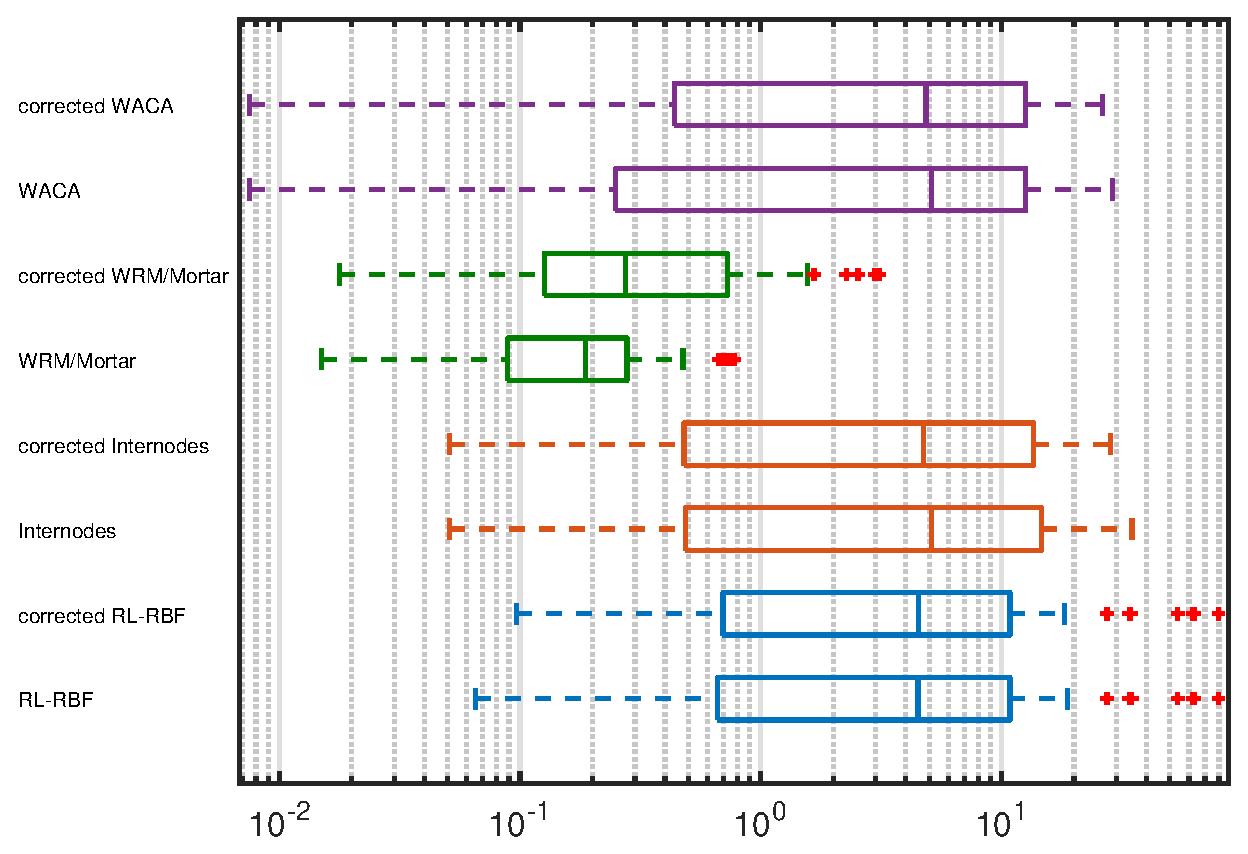
\includegraphics[width=0.7\linewidth]{images/Ch1/boxplot_EK}
 \caption{Boxplot of $E_K$, interface kinetic energy relative error.\label{fig.30}}
 \label{fig:boxplot_EK}
 \end{figure}
 
 Figure \ref{fig.30} results of all previous experiences are given also for $E_K \%$. We can see from these boxplots that further developments are still possible aimed at improving specifically the accuracy of the methods for dynamic problems.
\section{Advanced solver for FEA}
\subsection{Superelement exploitation}
\label{subsection1.4.1}
In the previous sections a 3D solid finite element formulation was considered. These, even if very general, suffer of strong limitations, when considering degenerated geometry, such as beam or shell geometries. In such structures linear solid elements suffer of some important shortcomings such as shear locking or computational burden. For this reason more specific component such as beam or shell elements have been developed in many FEM libraries. The Whole Engine Model (WEM) in our context is a very complex assembly of many different kinds of Elements, with many complicated loadings computed from both the engine manufacturer and the load analysis department. In such way of working the WEM needs to be considered with its contributions to loads and stiffness. These two contribute to the final measure of engine displacements that we want to monitor in this study.  The fact that an industrial engine model has to be integrated in the finite element analysis poses a real problem in terms of both implementation efficiency and development time since the combined engine and design zone structural model may be too complex and computationally expensive to be solved at each iteration of the optimization process. To circumvent these issues superelements \cite{nastran2013superelements} were employed. These are very efficient to deal with complex linear models that do not change in the optimization loop \cite{krog2004topology}.
Here we develop this method on a general structure shown in Figure \ref{f.3}.
\begin{figure}[hbt!]
\centering
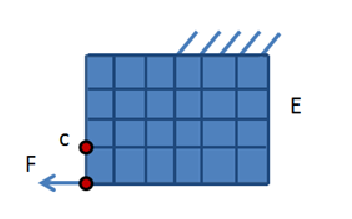
\includegraphics[width=.4\textwidth]{images/Ch1/dof_part.eps}
\caption{Example of DOFs partition: the nodes of the structure are sorted in retained nodes (whose DOFs are ($c$)) and other nodes (whose  DOFs are ($E$)). After the static condensation, a superelement containing only ($c$) DOFs will be generated. Nevertheless the suppressed DOFs ($E$) can still be computed after static analysis thanks to equation \ref{e.7}.  \label{f.3}}
\end{figure}
Sorting the structure's degrees of freedom into retained ($c$) and other degrees of freedom ($E$)\footnote{note that here ($E$) indicates only free DOFs and homogeneous Dirichlet conditions are considered.}, the static balance equation can then be written in the following form:
\begin{equation}
\label{e.6}
\left[ \begin{array}{cc}
\left[ \mathbf{K_{cc}} \right] & \left[ \mathbf{K_{cE}} \right]\\
\left[ \mathbf{K_{Ec}} \right] & \left[ \mathbf{K_{EE}} \right]
\end{array} \right] \left\lbrace \begin{array}{c}
\lbrace u_c \rbrace\\
\lbrace u_E \rbrace\\
\end{array}\right\rbrace =  \left\lbrace \begin{array}{c}
\lbrace F_c \rbrace\\
\lbrace F_E \rbrace\\
\end{array}\right\rbrace
\end{equation}
Using the second line block of equations and solving for $\lbrace u_E \rbrace$
\begin{equation}
\label{e.7}
\lbrace u_E \rbrace =\left[ P \right]\lbrace u_c \rbrace + \lbrace u_0 \rbrace
\end{equation}
With 
\begin{eqnarray}
\left[P\right]=-\left[ \mathbf{K_{EE}}\right]^{-1} \left[\mathbf{K_{Ec}}\right] \\
\lbrace u_0 \rbrace=\left[\mathbf{K_{EE}}\right]^{-1}\lbrace F_E \rbrace
\end{eqnarray}
The $\left[P\right]$ matrix is called constrained modal matrix in Nastran and recovery matrix in Abaqus. $\lbrace u_0 \rbrace$ is called fixed interface displacement on Nastran and has to be computed in a separated analysis on Abaqus.
Substituting   equation \ref{e.7} back in the first line block of \ref{e.6}:
\begin{equation}
\label{e.10}
\left[ \mathbf{\tilde{K}_{cc}}\right]\lbrace u_c \rbrace=\lbrace \tilde{F}_c \rbrace 
\end{equation}
With 
\begin{eqnarray}
\left[ \mathbf{\tilde{K}_{cc}}\right]=\left[\mathbf{K_{cc}}\right]+ \left[ P\right]^T\left[ \mathbf{K_{Ec}}\right] \\
\lbrace \tilde{F}_c \rbrace =\lbrace F_c \rbrace + \left[ P\right]^T\lbrace F_E \rbrace
\end{eqnarray}
In our problem we can make the evaluation of $ \left[ \mathbf{\tilde{K}_{cc}}\right]$ ,$\lbrace \tilde{F}_c \rbrace$ , $\left[ P\right]$ using a commercial software like Abaqus using the engine model. 
The $\lbrace u_0 \rbrace$ vector can also be evaluated using a linear perturbation static analysis of the engine, fixing the DOFs of the interface. If the structure has to be integrated into another model, the retained DOFs ($c$) can be used to describe the displacements of the whole assembly. The stiffness matrix of equation \ref{e.6} doesn't need to be inverted anymore, the only knowledge of $\left[\mathbf{\tilde{K}_{cc}}\right]$ and $\lbrace \tilde{F}_c \rbrace$ is sufficient.
Considering the engine interface DOFs as retained DOFs ($c$), we can make possible the evaluation of engine and design zone assembly displacements just considering the retained DOFs stiffness matrix and load vector. Using mesh tying techniques reviewed in section \ref{sec1.3} the engine retained nodes stiffness matrix and load vector can be integrated to the design zone.
In fact let's consider a simple elimination approach for the mesh tying of engine superelement and design zone finite element model.
  \begin{equation}
    \lbrace u_c \rbrace = \left[ \Pi_{cd} \right] \lbrace u_{d}\rbrace
    \end{equation}
Where $\lbrace u_c \rbrace$, $\lbrace u_{d}\rbrace $ are respectively engine and design zone interface DOFs.
After eliminating engine DOFs, the final system of equation reads :
    \begin{equation}
    \label{eq.1.119}
    \left[ \begin{array}{cc}
    \left[ \mathbf{K_{oo}} \right] & \left[ \mathbf{K_{od}} \right]\\
    \left[ \mathbf{K_{do}} \right] & \left[ \mathbf{K_{dd}} \right]+\left[ \Pi_{cd} \right]^T\left[ \mathbf{\tilde{K}_{cc}} \right]\left[ \Pi_{cd} \right]
    \end{array} \right] \left\lbrace \begin{array}{c}
    \lbrace u_o \rbrace\\
    \lbrace u_d \rbrace\\
    \end{array}\right\rbrace =  \left\lbrace \begin{array}{c}
    \lbrace F_o \rbrace\\
    \lbrace F_d\rbrace+\left[ \Pi_{cd} \right]^T\lbrace \tilde{F}_c\rbrace\\
    \end{array}\right\rbrace
    \end{equation} 
Where $o$ is the index of design zone DOFs not lying on the interface and:
\begin{equation}
\MatrixVar{\mathbf{K_{DZ}}}=\left[ \begin{array}{cc}
    \left[ \mathbf{K_{oo}} \right] & \left[ \mathbf{K_{od}} \right]\\
    \left[ \mathbf{K_{do}} \right] & \left[ \mathbf{K_{dd}} \right] 
    \end{array} \right] 
\end{equation}
Is the stiffness matrix relative to the Design Zone of the topology optimization problem and
\begin{equation}
\MatrixVar{\mathbf{K_{Eng}}}=\left[ \begin{array}{cc}
    \left[ 0 \right] & \left[ 0 \right]\\
    \left[ 0 \right] & \left[ \Pi_{cd} \right]^T\left[ \mathbf{\tilde{K}_{cc}} \right]\left[ \Pi_{cd} \right] 
    \end{array} \right] 
\end{equation} 
Is the engine superelement stiffness matrix.
The final system of equations in this case can then be written in a short form as :
\begin{equation}
\left(\MatrixVar{\mathbf{K_{Eng}}}+\MatrixVar{\mathbf{K_{DZ}}}\right)\VectorVar{U}=\MatrixVar{\mathbf{K}}\VectorVar{U}=\VectorVar{F}
\end{equation}
The superelement exploitation implies a significant economy in CPU time especially for big and complex engine models, since the full engine model does not have to be evaluated at each change of the design zone considered by the topology optimization. Furthermore, this also implies that the software used for evaluating the engine model can be separate from the one for evaluating the design zone model and carrying out the topology optimization. This is important since in practice the engine model is usually constructed in commercial FE software. In this work we used Abaqus for the engine model and Matlab for the design zone model and topology optimization. Accordingly reading Abaqus \textit{.dat} and \textit{.mtx} file from Matlab environment we can make the evaluation of the whole structure just using the Matlab environment as is summarized in figure \ref{f.6b}. Abaqus is used to generate both the engine and the design zone. A parsing of the input file is made on Matlab to import the design zone mesh coordinates and finite elements. The engine model is reduced to a superelement on the interface using Abaqus, then a parsing is made on the .mtx and the .dat file coming respectively from the sub-structuring and the linear load case. 
The stiffness matrix of the design zone is assembled together with the engine superelement stiffness matrix, the same is done for the load vectors. For each iteration of the topology optimization loop, the assembled problem is solved to determine the design zone displacements and the recovered engine displacements.  Finally tip clearance variations are computed in each stage and employed to compute consumption variation.
\begin{figure}[hbt!]
\centering
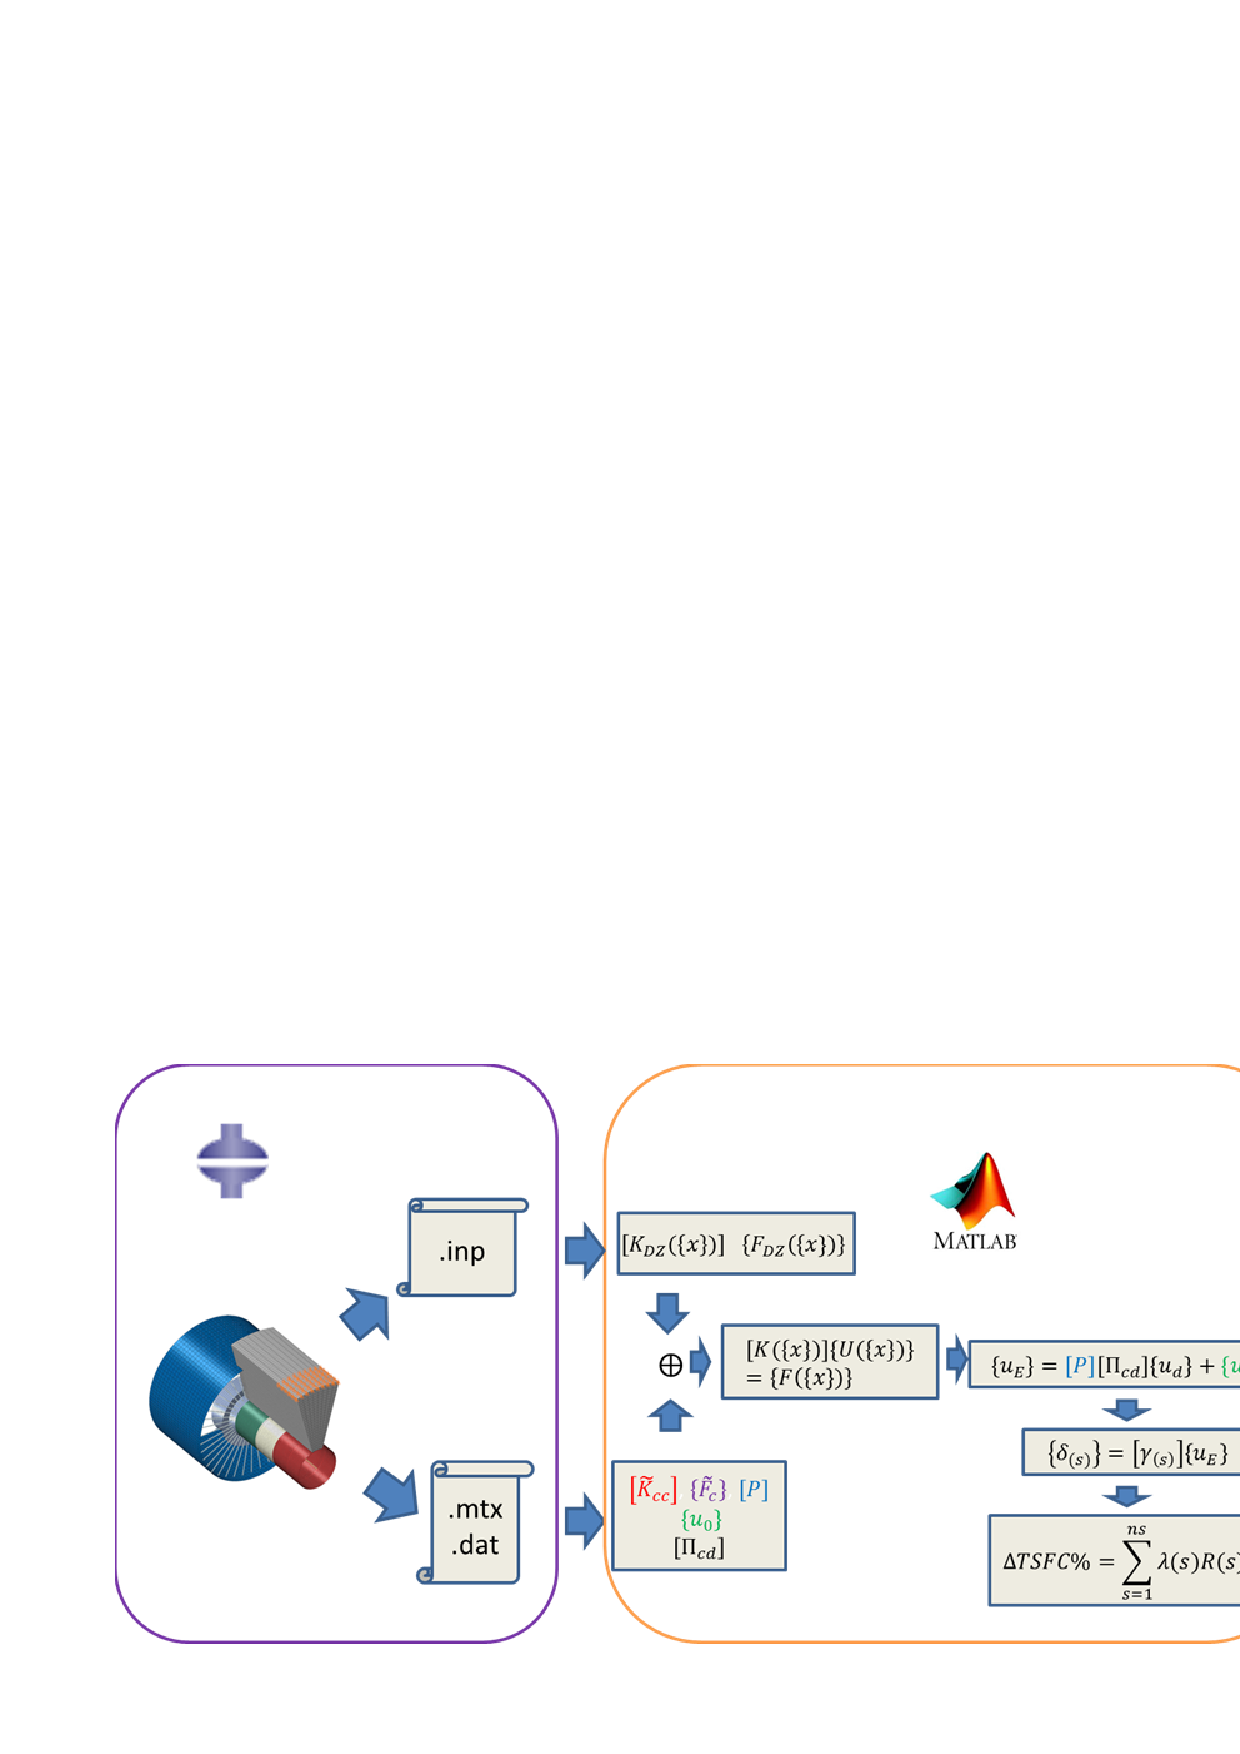
\includegraphics[width=0.85\textwidth]{images/Ch1/tip_cl_wkf.png}
\caption{Tip-clearance evaluation work-flow. 
\label{f.6b}}
\end{figure}
 This gives significant flexibility in implementing various approaches developed for topology optimization.
\subsection{Iterative solvers}
\label{subsection1.4.2}
Solving the balance equations \eqref{eq.1.119} for the free DOFs vector is an expensive task especially for large 3D problem as the one we try to tackle in this work. The stiffness matrix is large, sparse and positive definite. For this reason one can either employ direct solvers \cite{davis2006direct} or
iterative solvers \cite{saad2003iterative}. When dealing with small 2D problems, direct solvers are preferable due to their computational efficiency and robustness. In these approaches, the stiffness matrix is decomposed in the product of a lower triangular and an upper triangular matrices (LU or Choleski decompositions). Then, the resolution two systems of linear equations is carried out as a back substitution operation. For large scale 3D problems, these approaches become too expensive and ineffective \cite{davis2006direct}. For these cases, the sparsity of the stiffness matrix results in an inexpensive matrix vector product operation which can be effectively utilized by iterative solution algorithms.
\subsubsection{The Conjugate Gradient Algorithm}
 For symmetric positive definite matrices, a classic choice in terms of iterative solvers is the Conjugate Gradient (CG) algorithm \cite{hestenes1952methods}. Here we derive this algorithm following the procedure illustrated in \cite{saad2003iterative}. At each iteration $k$ of the Conjugate Gradient algorithm, the solution vector $\VectorVar{U}$ is updated as:
\begin{equation}
\VectorVar{U}_{(k+1)}=\VectorVar{U}_{(k)}+\alpha_{(k)}\VectorVar{p}_{(k)}
\end{equation}
where $\VectorVar{U}_{(k+1)}$ is the solution at the next iteration $k+1$ that is written in function of the solution at the previous iteration $\VectorVar{U}_{(k)}$, $\alpha_{(k)}$ is a scalar and $\VectorVar{p}_{(k)}$ is the perturbation direction at the same iteration $k$. One can define the residual vector $\VectorVar{r}$ defined at each iteration as:
\begin{equation}
\VectorVar{r}_{(k)}=\VectorVar{F}-\MatrixVar{\mathbf{K}}\VectorVar{U}_{(k)}
\end{equation}
The residual for the $k+1$ iteration can be then written as:
\begin{equation}
\VectorVar{r}_{(k+1)}=\VectorVar{F}-\MatrixVar{\mathbf{K}}\VectorVar{U}_{(k)}-\alpha_{(k)}\MatrixVar{\mathbf{K}}\VectorVar{p}_{(k)}=\VectorVar{r}_{(k)}-\alpha_{(k)}\MatrixVar{\mathbf{K}}\VectorVar{p}_{(k)}
\end{equation}
To enforce the residual at the iteration $k+1$ to be orthogonal to the one of the previous iteration $k$:
\begin{equation}
\VectorVar{r}_{(k+1)}^T \VectorVar{r}_{(k)}=0
\end{equation}
That is true only if:
\begin{equation}
\alpha_{(k)}=\frac{\VectorVar{r}_{(k)}^T\VectorVar{r}_{(k)}}{\VectorVar{r}_{(k)}^T\MatrixVar{\mathbf{K}}\VectorVar{p}_{(k)}}
\end{equation}
For the update of the search direction, one can ask that it has to belong to the span of vectors $\VectorVar{r}_{(k+1)}$ and $\VectorVar{p}_{(k)}$:
\begin{equation}
\label{eq.1.128}
\VectorVar{p}_{(k+1)}=\VectorVar{r}_{(k+1)} +\beta_{(k)}\VectorVar{p}_{(k)}
\end{equation}
To determine $\beta_{(k)}$ one has to enforce this time the orthogonality between $\VectorVar{p}_{(k+1)}$ and $\MatrixVar{\mathbf{K}}\VectorVar{p}_{(k)}$:
\begin{equation}
\label{eq.1.129}
\VectorVar{p}_{(k)}^T\MatrixVar{\mathbf{K}}\VectorVar{p}_{(k+1)}=0
\end{equation}
true only if:
\begin{equation}
\beta_{(k)}=-\frac{\VectorVar{p}_{(k)}^T\MatrixVar{\mathbf{K}}\VectorVar{r}_{(k+1)}}{\VectorVar{p}_{(k)}^T\MatrixVar{\mathbf{K}}\VectorVar{p}_{(k)}}
\end{equation}
Being:
\begin{equation}
\MatrixVar{\mathbf{K}}\VectorVar{p}_{(k)}=-\frac{1}{\alpha_{(k)}}\left(\VectorVar{r}_{(k+1)}-\VectorVar{r}_{(k)}\right)
\end{equation}
So that:
\begin{equation}
\beta_{(k)}=\frac{\VectorVar{r}_{(k+1)}^T\VectorVar{r}_{(k+1)}}{\alpha_{(k)}\VectorVar{p}_{(k)}^T\MatrixVar{\mathbf{K}}\VectorVar{p}_{(k)}}
\end{equation}
Using equations \eqref{eq.1.128} and \eqref{eq.1.129}:
\begin{equation}
\VectorVar{p}_{(k)}^T\MatrixVar{\mathbf{K}}\VectorVar{p}_{(k)}=\VectorVar{p}_{(k)}^T\MatrixVar{\mathbf{K}}\left(\VectorVar{r}_{(k)} +\beta_{(k-1)}\VectorVar{p}_{(k-1)}\right)=\VectorVar{p}_{(k)}^T\MatrixVar{\mathbf{K}}\VectorVar{r}_{(k)}
\end{equation}
then:
\begin{equation}
\beta_{(k)}=\frac{\VectorVar{r}_{(k+1)}^T\VectorVar{r}_{(k+1)}}{\VectorVar{r}_{(k)}^T\VectorVar{r}_{(k)}}
\end{equation}
The CG algorithm can then be written as:
\begin{algorithm}
\KwIn{$\MatrixVar{\mathbf{K}},\VectorVar{F},\varepsilon_{U}, N_{max}$}
\KwOut{$\VectorVar{U}_{(k)}$ approximation of the solution of $\MatrixVar{\mathbf{K}}\VectorVar{U}=\VectorVar{F}$ }

$k\gets 0$\;
$\VectorVar{U}_{(0)}\gets\VectorVar{0}$\;
$\VectorVar{r}_{(0)}\gets \VectorVar{F}$\;
$\VectorVar{p}_{(0)}\gets \VectorVar{r}_{(0)}$\;
 \While{$\frac{\|\VectorVar{r}_{(k)}\|_2}{\|\VectorVar{r}_{(0)}\|_2}\leq \varepsilon_{r}$ or $k\geq N_{max}$}{
 $\alpha_{(k)}\gets\frac{\VectorVar{r}_{(k)}^T\VectorVar{r}_{(k)}}{\VectorVar{p}_{(k)}^T\MatrixVar{\mathbf{K}}\VectorVar{p}_{(k)}}$\;
 $\VectorVar{U}_{(k+1)}\gets\VectorVar{U}_{(k)}+\alpha_{(k)}\VectorVar{p}_{(k)}$\;
$\VectorVar{r}_{(k+1)}\gets\VectorVar{r}_{(k)}-\alpha_{(k)}\MatrixVar{\mathbf{K}}\VectorVar{p}_{(k)}$\;
$\beta_{(k)}\gets\frac{\VectorVar{r}_{(k+1)}^T\VectorVar{r}_{(k+1)}}{\VectorVar{r}_{(k)}^T\VectorVar{r}_{(k)}}$\;
$\VectorVar{p}_{(k+1)}\gets\VectorVar{r}_{(k+1)} +\beta_{(k)}\VectorVar{p}_{(k)}$\;
  $k\gets k+1$\;
 }
 \KwRet{$\VectorVar{U}_{(k)}$}
 \caption{Conjugate Gradient \label{CG}}
\end{algorithm}
\subsubsection{The Preconditioned Conjugate Gradient (PCG) Algorithm}
It can be proven \cite{saad2003iterative} that CG reaches the solution vector $\VectorVar{U^*}$ in at most $n$ iterations\footnote{$n$ being the number of free DOFs i.e. the length of $\VectorVar{F}$.},and the convergence rate is shown to be:
\begin{equation}
\label{eq.1.135}
\|\VectorVar{U}_{(k)}-\VectorVar{U^*}\|_{\MatrixVar{\mathbf{K}}}\leq 2 \left(\frac{\sqrt{\kappa}-1}{\sqrt{\kappa}+1}\right)^k\|\VectorVar{U}_{0}-\VectorVar{U^*}\|_{\MatrixVar{\mathbf{K}}}
\end{equation}
where the $\MatrixVar{\mathbf{K}}$-norm of a vector is defined as:
\begin{equation}
\|\VectorVar{x}\|_{\MatrixVar{\mathbf{K}}}=\sqrt{\VectorVar{x}\MatrixVar{\mathbf{K}}\VectorVar{x}}
\end{equation}
$k$ is the iteration where the CG algorithm was stopped and $\kappa$ is the condition number of the stiffness matrix $\MatrixVar{\mathbf{K}}$. Equation \eqref{eq.1.135} shows that for $\kappa\gg 1$ the convergence of CG algorithm is very slow. In practice to accelerate and ensure convergence, preconditioning techniques are employed. The basic idea of these techniques is to replace the original system of equations by another one that has the same solution and is easier to be solved by iterative algorithms. An operator $\MatrixVar{\mathbf{M}}^{-1}$ has to be constructed so that $\kappa(\MatrixVar{\mathbf{M}}^{-1}\MatrixVar{\mathbf{K}}) \ll \kappa( \MatrixVar{\mathbf{K}})$.
By the use of such techniques the CG algorithm can be modified as in algorithm \ref{PCG}.
\begin{algorithm}[ht!]
\KwIn{$\MatrixVar{\mathbf{K}},\MatrixVar{\mathbf{M}}^{-1},\VectorVar{F},\varepsilon_{U}, N_{max}$}
\KwOut{$\VectorVar{U}_{(k)}$ approximation of the solution of $\MatrixVar{\mathbf{K}}\VectorVar{U}=\VectorVar{F}$ }

$k\gets 0$\;
$\VectorVar{U}_{(0)}\gets\VectorVar{0}$\;
$\VectorVar{r}_{(0)}\gets \VectorVar{F}$\;
$\VectorVar{z}_{(0)}\gets \MatrixVar{\mathbf{M}}^{-1} \VectorVar{r}_{(0)}$\;
$\VectorVar{p}_{(0)}\gets \VectorVar{z}_{(0)}$\;
 \While{$\frac{\|\VectorVar{r}_{(k)}\|_2}{\|\VectorVar{r}_{(0)}\|_2}\leq \varepsilon_{r}$ or $k\geq N_{max}$}{
 $\alpha_{(k)}\gets\frac{\VectorVar{r}_{(k)}^T\VectorVar{z}_{(k)}}{\VectorVar{p}_{(k)}^T\MatrixVar{\mathbf{K}}\VectorVar{p}_{(k)}}$\;
 $\VectorVar{U}_{(k+1)}\gets\VectorVar{U}_{(k)}+\alpha_{(k)}\VectorVar{p}_{(k)}$\;
$\VectorVar{r}_{(k+1)}\gets\VectorVar{r}_{(k)}-\alpha_{(k)}\MatrixVar{\mathbf{K}}\VectorVar{p}_{(k)}$\;
$\VectorVar{z}_{(k+1)}\gets\MatrixVar{\mathbf{M}}^{-1} \VectorVar{r}_{(k+1)}$\;
$\beta_{(k)}\gets\frac{\VectorVar{z}_{(k+1)}^T\VectorVar{r}_{(k+1)}}{\VectorVar{z}_{(k)}^T\VectorVar{r}_{(k)}}$\;
$\VectorVar{p}_{(k+1)}\gets\VectorVar{z}_{(k+1)} +\beta_{(k)}\VectorVar{p}_{(k)}$\;
  $k\gets k+1$\;
 }
 \KwRet{$\VectorVar{U}_{(k)}$}
 \caption{Preconditioned Conjugate Gradient \label{PCG}}
\end{algorithm}
One can observe that the application of the projection operator in \ref{PCG}, is needed once per iteration. For this reason a good preconditioning operator should be:
\begin{itemize}
\item Cheap: its application should not involve too many operations
\item Effective: $\kappa(\MatrixVar{\mathbf{M}}^{-1}\MatrixVar{\mathbf{K}})$ should be as close as possible to 1.
\item Scalable:  $\kappa(\MatrixVar{\mathbf{M}}^{-1}\MatrixVar{\mathbf{K}})$ and its computational burden should be proportional to the problem size $n$.
\item Robust:  $\MatrixVar{\mathbf{M}}^{-1}$ efficiency should not be problem dependent.
\item Simple:  complexity should be justified by the computational gain.
\end{itemize}
Among most common general purpose techniques we can find incomplete Cholesky Factorization \cite{kershaw1978incomplete}, the diagonal compensation \cite{jacobi1845ueber} and the Factorized Sparse Approximate Inverses (FSAI) \cite{buleev1960numerical,buleev1960numerical2,meijerink1977iterative,il1992iterative,varga1960boundary}. All these techniques are well adapted when the matrix of coefficients is not linked with a particular physics. In the next subsection we describe multi-grid approaches that take advantage from the fact that the matrix of coefficients comes from a PDE problem discretization.
\subsubsection{Multigrid Methods}
\label{multigrid}
The convergence of PCG for solving linear systems arising from PDE slows down with the size of the problem. Multigrid methods \cite{trottenberg2001multigrid} have been initially designed specifically to solve such problems. On the other hands these approaches' success is strongly dependent on the problem at hand and they need attention to get improved performances. They consist in the use of smoothers and coarse level corrections. 
Considering the residual decomposition over the basis of eigenvectors of the stiffness matrix, it can be shown that residual components associated with higher frequencies, are damped within few iterations by simple smoothing techniques like damped Jacobi, Gauss Seidel or Red-Black Gauss Seidel \cite{saad2003iterative}. On the other hand the low frequency components survive the smoothing step and need to be dealt with by coarse mesh corrections. The proofs of this results can be found in \cite{saad2003iterative}, for uniform 1D and 2D discretizations. In the present work we considered non uniform meshes, and this can be challenging for theoretical reasons, since one cannot directly transpose the considerations valid for uniform meshes to non-uniforms ones, and for practical reasons, since prolongation and interpolation operators may not be easily available. For this reason in the literature one can find Algebraic Multigrid (AMG) \cite{stuben2001review} that tries to emulate Geometric Multigrid (GMG) performance on the only knowledge of the coefficient matrix. In this work we focus our analysis on hierarchical non uniform hexahedral meshes.  This means that we considered fine meshes to be a consequence of a coarse mesh successive refinements. Each mesh refinement is considered as a level in the GMG.
In this way it is relatively simple to construct Interpolation and Prolongation operators to transfer vectors through levels.
Given a finite element of the coarse mesh, its refinement can be obtained cutting each finite element in 8 as shown in figures
\ref{f7},\ref{f8}.  
  \begin{figure}[hbt!]
  \centering
       \subfloat[ \label{fig.7a}]{%
                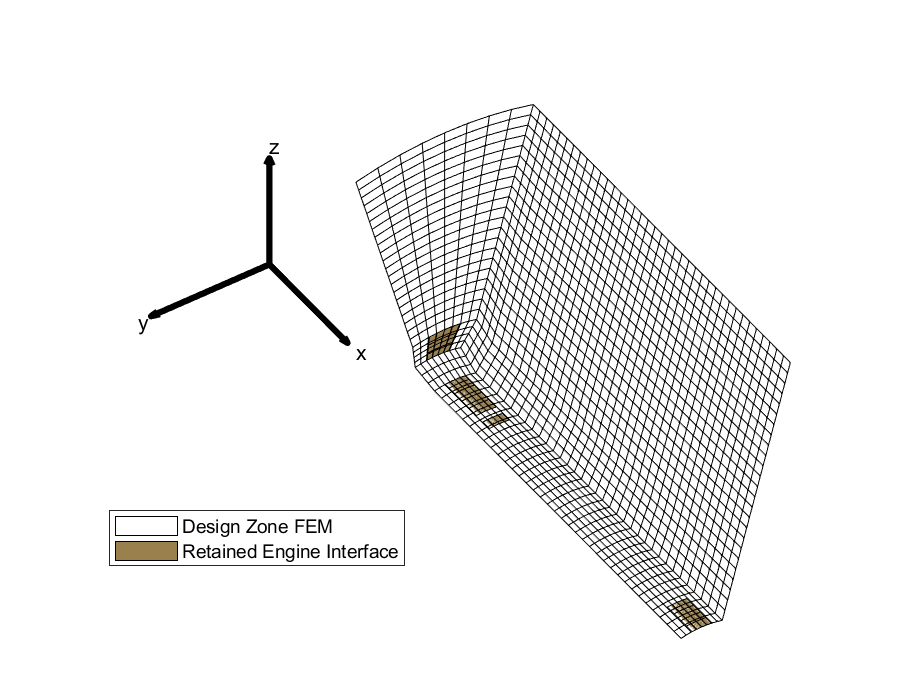
\includegraphics[width=0.5\textwidth]{images/Ch1/original_mesh.eps}
              }
       \subfloat[  \label{fig7b}]{%
         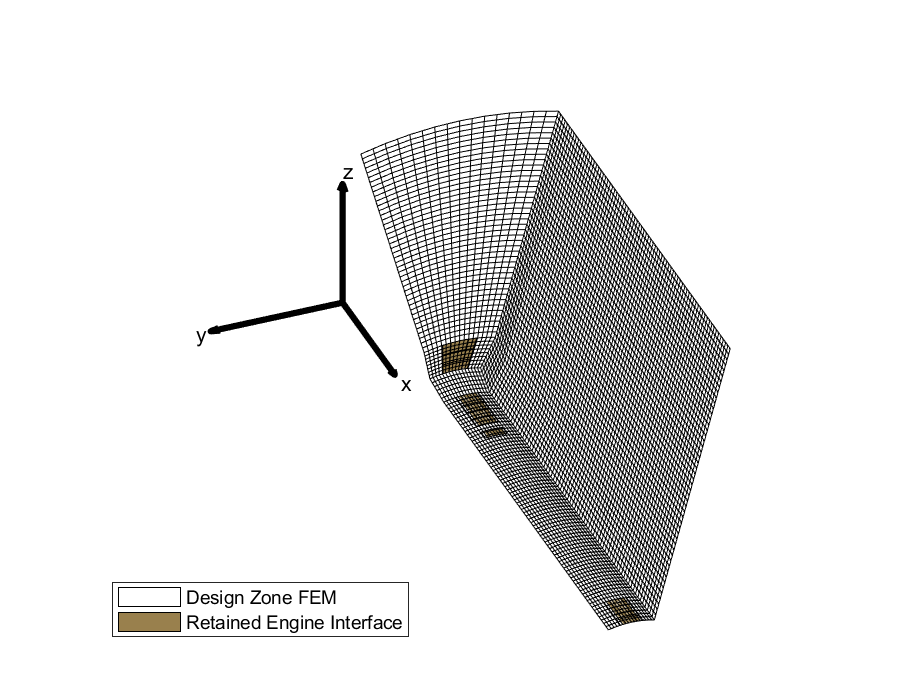
\includegraphics[width=0.5\textwidth]{images/Ch1/mesh_ref1.eps}
       }
       \caption{Mesh refinement procedure needed for multi-grid approach. The engine reduced element set is colored in yellow. Each node of these elements is kept in the engine superelement.(a) Original design zone mesh, generated in Abaqus and imported on matlab by input file parsing. The mesh counts 7600 8-node linear 3D solid finite elements and 9126 nodes. (b) Design zone mesh after refinement. Each element of the original element is cut in 8 new elements, that give a total of 7600$\times$8=60800 8-node linear 3D solid finite elements and  66759 nodes. }
       \label{f7}
     \end{figure} 
    \begin{figure}[hbt!]
        \centering
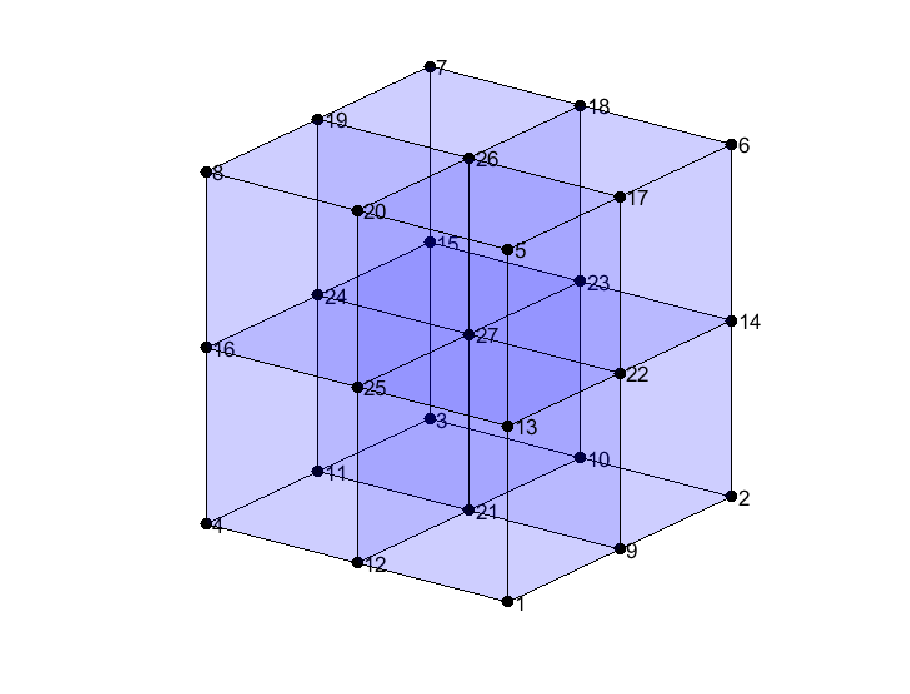
\includegraphics[width=0.5\textwidth]{images/Ch1/partition_3D.eps}
  \caption{3D partition employed for mesh refinement, nodes 1 to 8 belong to original coarse mesh element. Partition determines node 9 to 27 and 8 elements of the finer mesh.  }
       \label{f8}
     \end{figure}
     For each element of the coarse mesh we can define a transfer of the information between coarse level filed $u^c_i$ $i=1,2,...,8$ and the fine level field $u^f_j$ $j=1,2,...,27$, that can be used to construct the interpolation operator. 
     \begin{itemize}
     \item Node 1 to 8 of the fine mesh have their corresponding node in the coarse level so that: $u^c_i=u^f_i$ for $i=1,2,...,8$.
     \item Nodes 9 to 20 are in the middle of a coarse element edge. For this reason their field can be interpolated using the extremities of edges. For example $u^f_9=\frac{u^c_1+u^c_2}{2}$.
     \item Nodes 21 to 26 correspond to coarse element facet middle points. The corresponding component can be interpolated by the vertex of the corresponding coarse element facets. For instance $u^f_{21}=\frac{u^c_1+u^c_2+u^c_5+u^c_6}{4}$.
     \item Finally node 27 is in the coarse element centroid. Its nodal variable can be interpolated using all the coarse mesh node variables: $u^f_{27}=\frac{u^c_1+u^c_2+u^c_3+u^c_4+u^c_5+u^c_6+u^c_7+u^c_8}{8}$.
     \end{itemize}
        All previous relationships can be written in the matrix form: 
     \begin{equation}
     \VectorVar{u_f^{el}}=\MatrixVar{I_{fc}^{el}}\VectorVar{u_c^{el}}
     \end{equation}
     When considering the communication of several independent fields between each level one can use the same interpolation operator for each field:
     \begin{equation}
     \VectorVar{U_f^{el}}=\MatrixVar{I_{fc}^{el}\bigotimes I_d}\VectorVar{U_c^{el}}
     \end{equation}
     where $\bigotimes$ denotes the Kronecker product.
     Finally one can combine the equations coming from each coarse level element to build the global Interpolation operator. In doing so one has to consider each DOF of the fine mesh only once. Generally speaking the interpolation between the $l^{th}$ refinement and the corresponding coarser level is given by: 
      \begin{equation}
      \VectorVar{U_l}=\MatrixVar{I_{l,l-1}}\VectorVar{U_{l-1}}
      \end{equation}
      The prolongation operator allows for the inverse communication.  
 \begin{equation}
       \VectorVar{U_{l-1}}=\MatrixVar{P_{l-1,l}}\VectorVar{U_{l}}
 \end{equation}
 To keep the stiffness matrix at each refinement symmetric, the prolongation operator is considered to be:
 \begin{equation}
 \MatrixVar{P_{l-1,l}}=\MatrixVar{I_{l,l-1}}^T
 \end{equation}
 In this way given the state problem at the l-th refinement:
 \begin{equation}
 \MatrixVar{\mathbf{K_{l}}}\VectorVar{U_{l}}=\VectorVar{F_{l}}
 \end{equation}
 one can get a state problem at the coarser level as:
  \begin{equation}
  \MatrixVar{I_{l,l-1}}^T \MatrixVar{\mathbf{K_{l}}}\MatrixVar{I_{l,l-1}}\VectorVar{U_{l-1}}=\MatrixVar{\mathbf{K_{l-1}}}\VectorVar{U_{l-1}}=\MatrixVar{I_{l,l-1}}^T\VectorVar{F_{l}}=\VectorVar{F_{l-1}}
  \end{equation}
  This notation will be used to define the coarse mesh correction step needed in the multigrid. The other important ingredient plays a fundamental role in multigrid convergence is the smoothing.
  Here we will note:
  \begin{equation}
 \VectorVar{U_{l,\upsilon}}=\textit{smooth}^{\upsilon}(\MatrixVar{\mathbf{K_{l}}},\VectorVar{U_{l,0}},\VectorVar{F_{l}})
  \end{equation}
  where $\textit{smooth}^{\upsilon}$ denotes the application of $\upsilon$ steps of the form:
  \begin{equation}
 \VectorVar{ U_{l,j+1}}= \MatrixVar{\mathbf{B_{l}}}\VectorVar{U_{l,j}}+\MatrixVar{\mathbf{C_{l}}}\left(\VectorVar{F_{l}}\right)
  \end{equation}
  Where the matrix $\MatrixVar{\mathbf{B_{l}}}$ and $\MatrixVar{\mathbf{C_{l}}}$ depend on the particular approach chosen for the smoothing and will be detailed later. For two levels the multigrid algorithm can be encoded as in algorithm \ref{TGC}.
  \begin{algorithm}
 Pre-smooth: $\VectorVar{U_{l}}\gets\textit{smooth}^{\upsilon_1}(\MatrixVar{\mathbf{K_{l}}},\VectorVar{U_{l}},\VectorVar{F_{l}})$\;
 Get residual: $\VectorVar{r_{l}}\gets\VectorVar{F_{l}}-\MatrixVar{\mathbf{K_{l}}}\VectorVar{U_{l}}$\;
 Coarsen: $\VectorVar{r_{l-1}}\gets\MatrixVar{I_{l,l-1}}^T\VectorVar{r_{l}}$\;
 Solve: $\MatrixVar{\mathbf{K_{l-1}}}\VectorVar{\delta_{l-1}}=\VectorVar{r_{l-1}}$\;
 Correct: $\VectorVar{U_{l}}\gets\VectorVar{U_{l}}+\MatrixVar{I_{l,l-1}}\VectorVar{\delta_{l-1}}$\;
 Post-smooth: $\VectorVar{U_{l}}\gets\textit{smooth}^{\upsilon_2}(\MatrixVar{\mathbf{K_{l}}},\VectorVar{U_{l}},\VectorVar{F_{l}})$\;
   \caption{Two Grid cycle \label{TGC}}
  \end{algorithm}
Note that using this technique recursively, the algorithm moves to coarsen levels until the coarsest mesh is reached and direct solvers can indeed be employed to solve the corresponding state problem. Such idea is at the origin of the V-cycle (c.f. algorithm \ref{Vcy}).
  \begin{algorithm}
 Pre-smooth: $\VectorVar{U_{l}}\gets\textit{smooth}^{\upsilon_1}(\MatrixVar{\mathbf{K_{l}}},\VectorVar{U_{l}},\VectorVar{F_{l}})$\;
 Get residual: $\VectorVar{r_{l}}\gets\VectorVar{F_{l}}-\MatrixVar{\mathbf{K_{l}}}\VectorVar{U_{l}}$\;
 Coarsen: $\VectorVar{r_{l-1}}\gets\MatrixVar{I_{l,l-1}}^T\VectorVar{r_{l}}$\;
If $l=1$\;
 Solve: $\MatrixVar{\mathbf{K_{l-1}}}\VectorVar{\delta_{l-1}}=\VectorVar{r_{l-1}}$\;
 Else \;
 Recursion: $\VectorVar{\delta_{l-1}}\gets$V-cycle$(\MatrixVar{\mathbf{K_{l-1}}},\VectorVar{0},\VectorVar{r_{l-1}})$\;
End \;
 Correct: $\VectorVar{U_{l}}\gets\VectorVar{U_{l}}+\MatrixVar{I_{l,l-1}}\VectorVar{\delta_{l-1}}$\;
 Post-smooth: $\VectorVar{U_{l}}\gets\textit{smooth}^{\upsilon_2}(\MatrixVar{\mathbf{K_{l}}},\VectorVar{U_{l,0}},\VectorVar{F_{l}})$\;
   \caption{$\VectorVar{U_{l}}$=V-cycle$(\MatrixVar{\mathbf{K_{l}}},\VectorVar{U_{l}},\VectorVar{F_{l}})$ \label{Vcy}}
  \end{algorithm}
  One can observe that in the V-cycle only matrix times vector multiplications are introduced at each prolongation and interpolation step. This operator can be introduced in line 10 of PCG \ref{PCG}. The resulting algorithm also called Multigrid Conjugate Gradients) (MGCG) \cite{tatebe1994efficient,ashby1996parallel} depending on the smoother and the number of levels can be both robust and efficient for solving the linear system associated with the displacement evaluation in topology optimization \cite{amir2014multigrid,aage2017giga}. As aforementioned, the smother choice has to be complementary to the coarse mesh corrections in terms of residual error components. In the problem at hand, superelements and non-uniform meshes make this choice particularly important. Damped Jacobi iterations (c.f. \ref{DJs}) are inexpensive and effective options especially for large problems.
  \begin{algorithm}
 $\VectorVar{U_{l}}\gets\VectorVar{U_{l}}+\omega\MatrixVar{\mathbf{D_{l}}}^{-1}\left(\VectorVar{F_{l}}-\MatrixVar{\mathbf{K_{l}}}\VectorVar{U_{l}}\right)$\;
 \caption{Damped Jacobi smoother \label{DJs}}
  \end{algorithm}
  \clearpage
  Where $\MatrixVar{\mathbf{D_{l}}}$ is the diagonal matrix of $\MatrixVar{\mathbf{K_{l}}}$. 
   On the other hand bad mesh quality and static condensation can cause large positive out-of-diagonal terms in the final stiffness matrix that can make diagonal scaling ineffective. Another issue consists in the choice of the damping parameter $\omega$. Theoretical considerations can be applied for the uniform meshes as explained in \cite{saad2003iterative}. For non-uniform meshes and for superelements, the accurate choice of this parameter can be even more complicated \cite{bin2010geometric}.
   We can cite here other effective smoother techniques that can be employed instead of damped Jacobi iterations.
   The  multi-parameter Jacobi method that can be considered as the sequential application of Jacobi step with different values (c.f. algorithm \ref{MPJ}).
     \begin{algorithm}
     For $j=1,2,...,p$\;
    $\VectorVar{U_{l}}\gets\VectorVar{U_{l}}+\omega_j\MatrixVar{\mathbf{D_{l}}}^{-1}\left(\VectorVar{F_{l}}-\MatrixVar{\mathbf{K_{l}}}\VectorVar{U_{l}}\right)$\;
    End\;
    \caption{Multi-parameter Jacobi Method \label{MPJ}}
     \end{algorithm}
  Using such approach, the frequency range on which damping is effective can be amplified \cite{bin2009efficient}.
  One can also consider Gauss-Seidel Iterations. Given the decomposition:
  \begin{equation}
  \MatrixVar{\mathbf{K_{l}}}=\MatrixVar{\mathbf{D_{l}}}+\MatrixVar{\mathbf{L_{l}}}+\MatrixVar{\mathbf{L_{l}}}^T
  \end{equation}
  Where $\MatrixVar{\mathbf{L_{l}}}$ is the lower triangular part of $\MatrixVar{\mathbf{K_{l}}}$, then the Gauss-Seidel Iterations takes the form in algorithm \ref{GS}.
\begin{algorithm} 
       $\VectorVar{U_{l}}\gets\left(\MatrixVar{\mathbf{D_{l}}}+\MatrixVar{\mathbf{L_{l}}}\right)^{-1}\left(\VectorVar{F_{l}}-\MatrixVar{\mathbf{L_{l}}}^T\VectorVar{U_{l}}\right)$\;
       \caption{Gauss-Seidel smoother\label{GS}}
\end{algorithm}
For high dimensional problems the effectiveness of these approaches can be improved introducing a relaxation parameter $0<\omega<2$ that gives the Successive Over Relaxation (SOR)method (algorithm \ref{SOR}).
 \begin{algorithm} 
        $\VectorVar{U_{l}}\gets\left(\MatrixVar{\mathbf{D_{l}}}+\omega\MatrixVar{\mathbf{L_{l}}}\right)^{-1}\left(\omega\VectorVar{F_{l}}+\left((1-\omega)\MatrixVar{\mathbf{D_{l}}}-\omega\MatrixVar{\mathbf{L_{l}}}^T\right)\VectorVar{U_{l}}\right)$\;
        \caption{SOR smoother\label{SOR}}
 \end{algorithm}
Multi-parameter Jacobi principle can be extended to SOR approach. In this work we refer to this technique as Multi Parameter Successive Over Relaxation (MPSOR) (algorithm \ref{MPSOR}).
 \clearpage
 \begin{algorithm} 
 For $j=1,2,...,p$\;
        $\VectorVar{U_{l}}\gets\left(\MatrixVar{\mathbf{D_{l}}}+\omega_j\MatrixVar{\mathbf{L_{l}}}\right)^{-1}\left(\omega_j\VectorVar{F_{l}}+\left((1-\omega_j)\MatrixVar{\mathbf{D_{l}}}-\omega_j\MatrixVar{\mathbf{L_{l}}}^T\right)\VectorVar{U_{l}}\right)$\;
        EndFor\;
        \caption{MPSOR smoother\label{MPSOR}}
 \end{algorithm}
 For some problems all reviewed approaches may be not efficient, so that Incomplete decomposition smoothers (Ichol(0), ILU(0)) have to be considered. In our case, the stiffness matrix being symmetric:
 \begin{equation}
 \MatrixVar{\mathbf{K_{l}}}\approx \MatrixVar{\mathbf{\bar{L}_{l}}}\MatrixVar{\mathbf{\bar{L}_{l}}}^T
 \end{equation}
 where $\MatrixVar{\mathbf{\bar{L}_{l}}}$ is the incomplete Cholesky decomposition of the stiffness matrix. 
 The ICHOL smoother step is presented in algorithm \ref{ICHOL}.
 \begin{algorithm} 
      $\VectorVar{U_{l}}\gets\VectorVar{U_{l}}+\omega\MatrixVar{\mathbf{\bar{L}_{l}}}^{-1}{\MatrixVar{\mathbf{\bar{L}_{l}}}}^{-T}\left(\VectorVar{F_{l}}-\MatrixVar{\mathbf{K_{l}}}\VectorVar{U_{l}}\right)$\;
         \caption{ICHOL smoother\label{ICHOL}}
  \end{algorithm}
 Smoothers like ICHOL and damped Jacobi can also be written as:
 \begin{equation}
 \VectorVar{U_{l}}_{k+1}=\VectorVar{U_{l}}_{k}+\omega_k\VectorVar{\delta_{l}}_{k+1}
 \end{equation}
 Common choices of damping parameter $\omega$ are based on experience or theoretical principles for Damped Jacobi, in order to be complementary with coarse mesh correction. In topology optimization this can represent a challenge since each configuration has a different stiffness matrix and potentially several optimal $\omega$. To make a reasonable choice of the damping parameter here we consider that smoother efficiency could be related to the residual 2-norm after the smoothing step. If this is looked as part of a deepest descent algorithm, then the $\omega$ value can be obtained as the result of a line-search minimization of the residual 2-norm over the descent direction. 
  \begin{algorithm} 
  Compute $\VectorVar{\delta_{l}}$ and $\VectorVar{\hat{\delta}_{l}}=\MatrixVar{\mathbf{K_{l}}}\VectorVar{\delta_{l}}$\;
  $\VectorVar{r_{l}}\gets\VectorVar{F_{l}}-\MatrixVar{\mathbf{K_{l}}}\VectorVar{U_{l}}$\;
  	$\omega\gets\frac{\VectorVar{r_{l}}^T\VectorVar{\hat{\delta}_{l}}}{\VectorVar{\hat{\delta}_{l}}^T\VectorVar{\hat{\delta}_{l}}}$\;
       $\VectorVar{U_{l}}\gets\VectorVar{U_{l}}+\omega\VectorVar{\delta_{l}}$\;
          \caption{Line Search $\omega$ update\label{LS}}
   \end{algorithm}
 \\
 This method is not theoretically proven to be more effective than constant $\omega$ counterpart but in our experience can provide results that are comparable with an optimal constant choice of $\omega$. This comes at the cost of a more expensive computation of the smoother since a matrix-vector and 2 scalar products have to be computed to use this scheme. When the algorithm \ref{LS} is adopted together with a reviewed smoother we will refer to LS-Ichol and LS-Jacobi. The most suitable smother should then be selected on the base of tests made on a given configuration.  
 \subsubsection{Multigrid tuning and smoothers benchmark}
 As it was stated in the previous subsection, multigrid efficiency comes with the loss of solver robustness. In fact smoother tuning and selection is a problem dependent choice.
 In this section we try several combinations of coarse mesh corrections and of smoothers to get faster convergence on the finite element model presented in chapters \ref{chap:2} and \ref{chap:3} for three load cases. The design region's Young Modulus is the one of the full material (Iron) for each finite element.
 We are limiting our attention to Damped Jacobi, Ichol, SOR, LS-Jacobi and LS Ichol smoothers. We considered the same number of pre and post smoothing: $\upsilon_1=\upsilon_2=\upsilon$. We considered only 1 or two sweeping. For Line Search variants the value of $\omega$ was computed for each sweeping step on the other hand for simple variants we investigated
 \begin{eqnarray}
\omega_{Jacobi}\in[0.2,0.5]\\
\omega_{SOR} \in [0.4,1.6]\\
\omega_{Ichol} \in [0.9,1.2]
 \end{eqnarray}
 The convergence criterion was based on the maximum of the $L^2$-norm of each load case's residual and on the maximum number of iterations:
 \begin{eqnarray}
 r_r=\frac{max_i\|\VectorVar{r_{IT,i}}\|_2}{max_i\|\VectorVar{r_{0,i}}\|_2}\leq 10^{-5}\\
  IT\leq 10^{2}
 \end{eqnarray}
 where $ r_r$ is referred to as relative residual.
  The 3 load cases were solved simultaneously adapting the original Matlab code of \cite{amir2014multigrid}.
 We then compared the results in terms of Iterations at convergence, CPU total time $T_{tot}$, the average residual reduction per iteration and convergence speed. We indicate the average residual reduction per iteration, the coefficient that reduces residual norm at each iteration:
 \begin{equation}
 \label{eq.arr}
 ARR=\left(\frac{max_i\|\VectorVar{r_{0,i}}\|_2}{max_i\|\VectorVar{r_{IT,i}}\|_2}\right)^{\frac{1}{IT}}
 \end{equation}
 where $\VectorVar{r_{0,i}}$ indicates the residual of load case $i$ at iteration 0, and $\VectorVar{r_{IT,i}}$ indicates the residual of load case $i$ at the last iteration $IT$.
 One can say that at each iteration the residual norm in average is reduced by $ARR$ times. That is still an incomplete piece of information because the evaluation time per iteration is not considered.
  We refer then to convergence speed measured in Hertz or reductions per second  as:
 \begin{equation}
 \label{eq.cs}
 C_S=-\frac{IT \log\left(ARR\right)}{T_{it}}
 \end{equation}
 where $T_{it}$ is the CPU time in seconds of the iterative approach that grows with the PCG iterations. In fact the time needed for the incomplete and full Cholesky decomposition of stiffness matrices in each level has to be conducted just once before PCG iterations. The $C_S$ parameter is considered the average convergence ratio over the whole convergence. If the convergence history had an exponential form with respect to the computational time from the beginning of iteration $t$ it would have the form of:
 \begin{equation}
 max_i\|\VectorVar{r_{IT,i}}\|_2(t)=max_i\|\VectorVar{r_{0,i}}\|_2e^{-C_St}
 \end{equation}
 The higher the $C_S$, the faster is the convergence for the same accuracy. 
  Finally the total CPU time here mentioned as ${T_{tot}}$ include both the part coming from iterations and the part coming from decompositions.
   \begin{figure}[hbt!]
   \centering
        \subfloat[ \label{fig.1.32a}]{%
                 \includegraphics[width=0.5\textwidth]{code_matlab/Iterations_Damped_Jacobi.eps}
               }
        \subfloat[  \label{fig.1.32b}]{%
          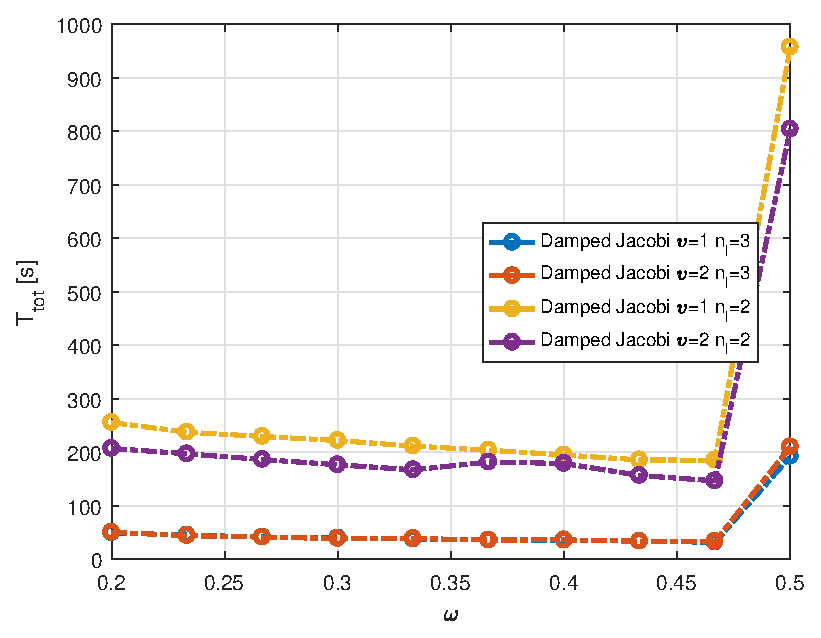
\includegraphics[width=0.5\textwidth]{code_matlab/cputime_Damped_Jacobi.eps}
        }\\
        \subfloat[ \label{fig.1.32c}]{%
          \includegraphics[width=0.5\textwidth]{code_matlab/convergence_speed_Damped_Jacobi.eps}
                       }
        \subfloat[  \label{fig.1.32d}]{%
           \includegraphics[width=0.5\textwidth]{code_matlab/ARR_Damped_Jacobi.eps}
                }
        \caption{Damped Jacobi smoother performances as a function of $\omega$ and for different numbers of mesh levels $n_l$, different numbers of sweeping $\upsilon$. (a) Iterations at convergence.(b) CPU time [s]. (c) Convergence speed defined in equation [Hz] \eqref{eq.cs}. (d) Average Residual Reduction per iteration defined in equation \eqref{eq.arr}. }
        \label{f.1.32}
      \end{figure} 
      In figure \ref{f.1.32} the performances of damped Jacobi smoother are computed for several values of $\omega$, mesh levels $n_l$ and different numbers of sweeping $\upsilon$. One can observe that the minimal CPU time $\approx33$ seconds is reached for $n_l=3$, $\upsilon=2$, $\omega\approx0.47$. 
      One can observe that for $\omega=0.5$ and $\upsilon=1$ the desired accuracy for the relative residual was not reached within 100 iterations. 
      The maximal convergence speed was of $0.35 Hz$, that makes the error reduced by 2.7 at each iteration ( c.f. figure \ref{fig.1.32d}).
       \begin{figure}[hbt!]
         \centering
              \subfloat[ \label{fig.1.33a}]{%
                       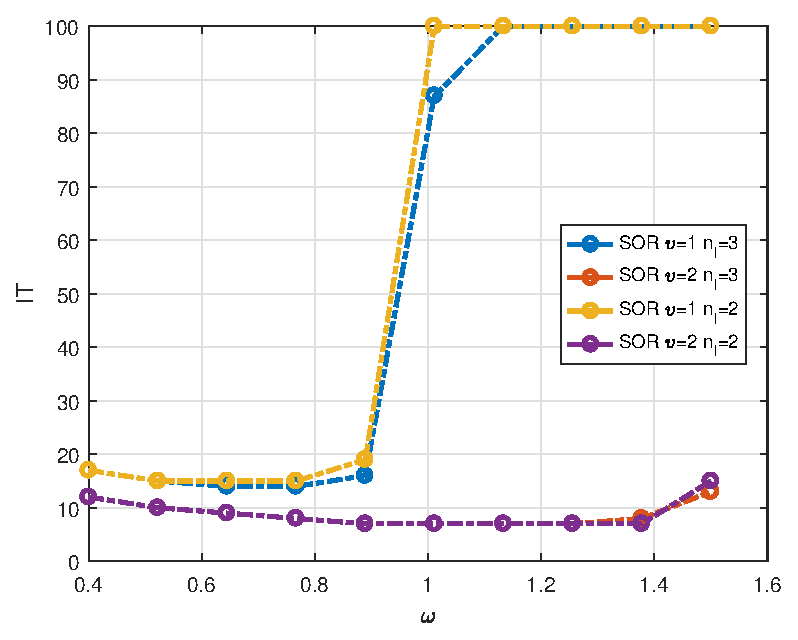
\includegraphics[width=0.5\textwidth]{code_matlab/Iterations_SOR.eps}
                     }
              \subfloat[  \label{fig.1.33b}]{%
                \includegraphics[width=0.5\textwidth]{code_matlab/cputime_SOR.eps}
              }\\
              \subfloat[ \label{fig.1.33c}]{%
                \includegraphics[width=0.5\textwidth]{code_matlab/convergence_speed_SOR.eps}
                             }
              \subfloat[  \label{fig.1.33d}]{%
                 \includegraphics[width=0.5\textwidth]{code_matlab/ARR_SOR.eps}
                      }
              \caption{SOR smoother performances as a function of $\omega$ and for different numbers of mesh levels $n_l$, different numbers of sweeping $\upsilon$. (a) Iterations at convergence.(b) CPU time [s]. (c) Convergence speed defined in equation [Hz] \eqref{eq.cs}. (d) Average Residual Reduction per iteration defined in equation \eqref{eq.arr}.}
              \label{f.1.33}
            \end{figure}
            SOR smoother performances were reported in figure \ref{f.1.33}. In figures \ref{fig.1.33a}  and \ref{fig.1.33b} one can observe a strong dependency of the convergence with the number of sweeping. In fact for $\upsilon=1$ and for $\omega\geq 1$ PCG didn't converged within 100 iterations. The best convergence is obtained for $\omega\approx1.13$, $\upsilon=2$ and $n_l=3$ with 7 iterations in 31 seconds. In figures \ref{fig.1.33c}  and \ref{fig.1.33d} one can also observe that for this point the convergence speed is of $C_S\approx0.4Hz$ and the $ARR\approx6$. This investigation seems to suggest that one could improve performances increasing the number of levels and increasing the number of sweeping. 
            \begin{figure}[hbt!]
                     \centering
                          \subfloat[ \label{fig.1.34a}]{%
                                   \includegraphics[width=0.5\textwidth]{code_matlab/Iterations_Ichol.eps}
                                 }
                          \subfloat[  \label{fig.1.34b}]{%
                            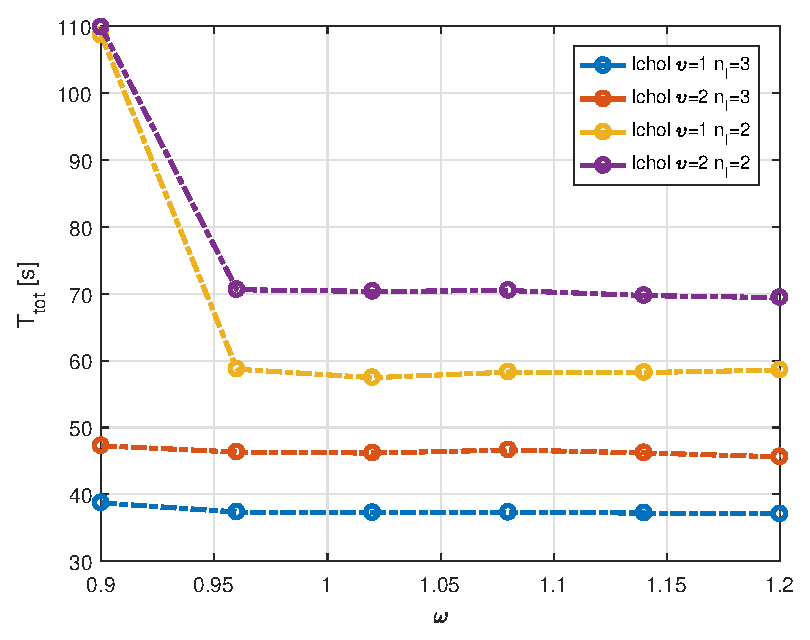
\includegraphics[width=0.5\textwidth]{code_matlab/cputime_Ichol.eps}
                          }\\
                          \subfloat[ \label{fig.1.34c}]{%
                            \includegraphics[width=0.5\textwidth]{code_matlab/convergence_speed_Ichol.eps}
                                         }
                          \subfloat[  \label{fig.1.34d}]{%
                             \includegraphics[width=0.5\textwidth]{code_matlab/ARR_Ichol.eps}
                                  }
                          \caption{Ichol smoother performances as a function of $\omega$ and for different numbers of mesh levels $n_l$, different numbers of sweeping $\upsilon$. (a) Iterations at convergence.(b) CPU time [s]. (c) Convergence speed defined in equation [Hz] \eqref{eq.cs}. (d) Average Residual Reduction per iteration defined in equation \eqref{eq.arr}. }
                          \label{f.1.34}
                        \end{figure}  
                        Ichol smoother performances are described in figure \ref{f.1.34}.  For this method the CPU time include the computation of incomplete Cholesky decompositions for each level. One can observe that much less PCG iterations are needed up to convergence ($\leq 5$). The CPU time per iteration is on the other hand very high and reaches its minimum of 37 seconds for $\omega\approx1.12$ $n_l=3$ and $\upsilon=1$. The maximum convergence speed is reached for the same point $C_S\approx 0.64 Hz$ and is bigger than the value found for the other methods. This means that Ichol smoother has a fast convergence, but still the investment required for the construction of preconditioning is not justified for the accuracy of $10^{-5}$. That is why finally the SOR optimal point is still better than the Ichol point if we look at the total CPU time. If we consider the Line Search variants for Damped Jacobi and Ichol smoother (cf. table \ref{tab:1.1}) we can observe that the fastest combinations are for $\upsilon=1$ and $n_l=3$. The best approach found for this configuration was the LS variant of Ichol with $T_{tot}\approx 37$ seconds. Still this approach is less interesting then Ichol in terms of convergence speed. For a general conclusion based on this configuration, depending on the accuracy needed ichol and LS-ichol smoothers can be effective for applications where strict accuracy is demanded so that the investment on the initial evaluation of the incomplete Cholesky decomposition is repaid by the improved convergence speed. On the other hand SOR and damped Jacobi are very inexpensive and can be adopted in situations where the final accuracy is less critical. Another important criterion of selection that is out of the scope of this work is the scalability of the preconditioner.
                        \begin{table}[h!]
                        % table caption is above the table
                        \caption{Performance of Line Search variants}
                        \label{tab:1.1}       % Give a unique label
                        \centering
                        % For LaTeX tables use
                        \begin{tabular}{lllllll}
                        \hline\noalign{\smallskip}
                        Method & $\upsilon$ & $n_l$ & $IT$ & $T_{tot} [s]$ & $C_S [Hz]$ & $ARR$\\
                        \noalign{\smallskip}\hline\noalign{\smallskip}
                        LS-Damped Jacobi & 1 & 2 & 12 & 53.1 & 0.2348 & 2.78 \\
                        LS-Damped Jacobi & 2 & 2 & 11 & 169.9 & 0.0892 & 2.89 \\
                        LS-Damped Jacobi & 1 & 3 & 18 & 50.5 & 0.2421 & 1.95 \\
                        LS-Damped Jacobi & 2 & 3 & 17 & 208.8 & 0.0699 & 2.01 \\
						LS-Ichol & 1 & 2 & 4 & 52.9 & 0.3384 & 23.1 \\
                        LS-Ichol & 2 & 2 & 4 & 114 & 0.2348 & 39.4 \\
                        LS-Ichol & 1 & 3 & 4 & 37 & 0.5452 & 17.8 \\
                        LS-Ichol & 2 & 3 & 4 & 99.5 & 0.2635 & 23.5 \\
                        \noalign{\smallskip}\hline
                        \end{tabular}
                        \end{table}
\section{Summary and conclusions}      
In this chapter the Finite Element Model approach was reviewed for the resolution of linear elastostatics problems. The optimization framework that is developed in this PhD requires in fact the reliable and fast evaluation of displacements, tip-clearance and stress in a large finite element model including both design space and engine models. In the introduction we also detailed the challenges that this simulation problem represented.  The engine model can be large and complex, to make it available in our Matlab framework, the exploitation of superelements was first reviewed. The design space being meshed in an external environment, 8 node full integration hexahedral elements were reviewed. This gives the freedom to mesh mappable design space geometries that can easily satisfy aerodynamic and integration constraints. The communication between design space mesh and engine model is delicate since discretizations are not consistent at the interface. Several techniques were reviewed and compared with  a new technique we proposed. To make the evaluation of model responses faster in the optimization loop, multigrid preconditioned conjugate gradient was implemented and tested with several smoothers. To summarize the review in this chapter recovered the following topics :
\begin{itemize}
\item Finite Element notation
\item Mesh tying
\item Superelements
\item Multigrid preconditioners
\end{itemize}
A personal contribution was given in:
\begin{itemize}
\item Weighted Average Continuity Approach (WACA) and Moment correction were proposed to deal with mesh tying related issues. Their performances were compared with reviewed approaches on simple 3D examples. Moment correction sensibly improves displacement or stress accuracy of all reviewed technique. Its implementation is recommended in Structural Finite Element models with mesh tying to enforce the local mechanical moment balance at the tied interface. 
\item This work led to the publication of a journal article \cite{coniglio2018weighted}.
\item Different smoother techniques were reviewed and benchmarked on a  demonstration example that includes non-uniform hexahedral elements and the engine superelement for a 3 right hand side vectors application.
\end{itemize}
The studies conducted in this chapter show that our framework, using a combination of reviewed techniques and proposed approaches, provides accurate and relatively fast responses that can be considered consistent with modeling hypothesis.
As possible axes of improvement we can cite:
\begin{itemize}
\item Distributed memory implementations of the provided framework could also be considered as a valid improvement axis. 
\item Other important issue like shear locking control could be introduced in order to improve finite element accuracy.
\item  Still, the major limitation of the proposed framework consists in the fact that the WEM needs to be a linear model to be imported as a superelement. A possible solution in case of nonlinear engine models could be provided by non-intrusive coupling techniques \cite{Gendre2009}.
\end{itemize}
%%% Local Variables: 
%%% mode: latex
%%% TeX-master: "../phdthesis"
%%% End:

% \chapter{Structural and Topology optimization}
\label{sec:unchapitre}
\minitoc

Lorem ipsum dolor sit amet, consectetur adipiscing elit \cite{Bello1963}. Sed non risus. Suspendisse lectus tortor, dignissim sit amet, adipiscing nec, ultricies sed, dolor. Cras elementum ultrices diam. Maecenas ligula massa, varius a, semper congue, euismod non, mi. Proin porttitor, orci nec nonummy molestie, enim est eleifend mi, non fermentum diam nisl sit amet erat. Duis semper. Duis arcu massa, scelerisque vitae, consequat in, pretium a, enim. Pellentesque congue. Ut in risus volutpat libero pharetra tempor. Cras vestibulum bibendum augue. Praesent egestas leo in pede. Praesent blandit odio eu enim. Pellentesque sed dui ut augue blandit sodales. Vestibulum ante ipsum primis in faucibus orci luctus et ultrices posuere cubilia Curae; Aliquam nibh. Mauris ac mauris sed pede pellentesque fermentum. Maecenas adipiscing ante non diam sodales hendrerit. Ut velit mauris, egestas sed, gravida nec, ornare ut, mi. Aenean ut orci vel massa suscipit pulvinar. Nulla sollicitudin. 

\begin{figure}[htp!]
  \centering
  \setlength\figureheight{7cm}
  \setlength\figurewidth{9cm}
  \input{images/tikz_plot}
  \caption{Exemple de courbe TikZ.}
  \label{fig:courbe-tikz}
\end{figure}

\section{Description du modèle}

Lorem ipsum dolor sit amet, consectetur adipiscing elit. Sed non risus. Suspendisse lectus tortor, dignissim sit amet, adipiscing nec, ultricies sed, dolor. Cras elementum ultrices diam. Maecenas ligula massa, varius a, semper congue, euismod non, mi. Proin porttitor, orci nec nonummy molestie, enim est eleifend mi, non fermentum diam nisl sit amet erat. Duis semper. Duis arcu massa, scelerisque vitae, consequat in, pretium a, enim. Pellentesque congue. Ut in risus volutpat libero pharetra tempor. Cras vestibulum bibendum augue. Praesent egestas leo in pede. Praesent blandit odio eu enim. Pellentesque sed dui ut augue blandit sodales. Vestibulum ante ipsum primis in faucibus orci luctus et ultrices posuere cubilia Curae; Aliquam nibh. Mauris ac mauris sed pede pellentesque fermentum. Maecenas adipiscing ante non diam sodales hendrerit. Ut velit mauris, egestas sed, gravida nec, ornare ut, mi. Aenean ut orci vel massa suscipit pulvinar. Nulla sollicitudin. Fusce varius, ligula non tempus aliquam, nunc turpis ullamcorper nibh, in tempus sapien eros vitae ligula. 

Pellentesque rhoncus nunc et augue. Integer id felis. Curabitur aliquet pellentesque diam. Integer quis metus vitae elit lobortis egestas. Lorem ipsum dolor sit amet, consectetuer adipiscing elit. Morbi vel erat non mauris convallis vehicula. Nulla et sapien. Integer tortor tellus, aliquam faucibus, convallis id, congue eu, quam. Mauris ullamcorper felis vitae erat. Proin feugiat, augue non elementum posuere, metus purus iaculis lectus, et tristique ligula justo vitae magna. Aliquam convallis sollicitudin purus. Praesent aliquam, enim at fermentum mollis, ligula massa adipiscing nisl, ac euismod nibh nisl eu lectus. Fusce vulputate sem at sapien. Vivamus leo. Aliquam euismod libero eu enim. Nulla nec felis sed leo placerat imperdiet. Aenean suscipit nulla in justo. Suspendisse cursus rutrum augue. Nulla tincidunt tincidunt mi. Curabitur iaculis, lorem vel rhoncus faucibus, felis magna fermentum augue, et ultricies lacus lorem varius purus. Curabitur eu amet.

\section{Analyse aux limites}

Lorem ipsum dolor sit amet, consectetur adipiscing elit. Sed non risus. Suspendisse lectus tortor, dignissim sit amet, adipiscing nec, ultricies sed, dolor. Cras elementum ultrices diam. Maecenas ligula massa, varius a, semper congue, euismod non, mi. Proin porttitor, orci nec nonummy molestie, enim est eleifend mi, non fermentum diam nisl sit amet erat. Duis semper. Duis arcu massa, scelerisque vitae, consequat in, pretium a, enim. Pellentesque congue. Ut in risus volutpat libero pharetra tempor. Cras vestibulum bibendum augue. Praesent egestas leo in pede. Praesent blandit odio eu enim. Pellentesque sed dui ut augue blandit sodales. Vestibulum ante ipsum primis in faucibus orci luctus et ultrices posuere cubilia Curae; Aliquam nibh. Mauris ac mauris sed pede pellentesque fermentum.

\subsection{Calculer en cent leçons}

Lorem ipsum dolor sit amet, consectetuer adipiscing elit. Morbi vel erat non mauris convallis vehicula. Nulla et sapien. Integer tortor tellus, aliquam faucibus, convallis id, congue eu, quam. Mauris ullamcorper felis vitae erat. Proin feugiat, augue non elementum posuere, metus purus iaculis lectus, et tristique ligula justo vitae magna. Aliquam convallis sollicitudin purus. Praesent aliquam, enim at fermentum mollis, ligula massa adipiscing nisl, ac euismod nibh nisl eu lectus. Fusce vulputate sem at sapien. Vivamus leo. Aliquam euismod libero eu enim. Nulla nec felis sed leo placerat imperdiet. Aenean suscipit nulla in justo. Suspendisse cursus rutrum augue. Nulla tincidunt tincidunt mi. Curabitur iaculis, lorem vel rhoncus faucibus, felis magna fermentum augue, et ultricies lacus lorem varius purus. Curabitur eu amet.

\subsection{Le monde conique}

Lorem ipsum dolor sit amet, consectetuer adipiscing elit. Morbi vel erat non mauris convallis vehicula. Nulla et sapien. Integer tortor tellus, aliquam faucibus, convallis id, congue eu, quam. Mauris ullamcorper felis vitae erat. Proin feugiat, augue non elementum posuere, metus purus iaculis lectus, et tristique ligula justo vitae magna. Aliquam convallis sollicitudin purus. Praesent aliquam, enim at fermentum mollis, ligula massa adipiscing nisl, ac euismod nibh nisl eu lectus. Fusce vulputate sem at sapien. Vivamus leo. Aliquam euismod libero eu enim. Nulla nec felis sed leo placerat imperdiet. Aenean suscipit nulla in justo. Suspendisse cursus rutrum augue. Nulla tincidunt tincidunt mi. Curabitur iaculis, lorem vel rhoncus faucibus, felis magna fermentum augue, et ultricies lacus lorem varius purus. Curabitur eu amet.

\begin{align}
H_{m,n,p,q} &= \DPR{\rproto_{p,q}}{\OP{H} \tproto_{m,n}}\\
&= \iint\limits_{\SET{R}^2} S_{\OP{H}}(f,\tau) \DPR{\rproto_{p,q}}{\OP{U}_{f,\tau} \tproto_{m,n}} \ud f \ud \tau \\
&= \iint\limits_{\SET{R}^2} S_{\OP{H}}(f,\tau) \int\limits_{\R} \rproto_{p,q}^*(t) \OP{U}_{f,\tau} (\tproto_{m,n})(t) \ud t \ud f \ud \tau\\
&= \iint\limits_{\SET{R}^2} S_{\OP{H}}(f,\tau) \int\limits_{\R} \rproto^*(t-qT_0)e^{-j2 \pi pF_0t} \tproto(t-nT_0-\tau)e^{j2 \pi (mF_0(t-\tau) + ft)} \ud t \ud f \ud \tau\\
&= \iint\limits_{\SET{R}^2} S_{\OP{H}}(f,\tau) e^{-j2\pi m F_0 \tau} \int\limits_{\R} \rproto^*(t-qT_0) \tproto(t-nT_0-\tau)e^{j2 \pi ((m-p)F_0 + f)t} \ud t \ud f \ud \tau.
\end{align}

\section{Vérification par simulation numérique}

Lorem ipsum dolor sit amet, consectetur adipiscing elit. Sed non risus. Suspendisse lectus tortor, dignissim sit amet, adipiscing nec, ultricies sed, dolor. Cras elementum ultrices diam. Maecenas ligula massa, varius a, semper congue, euismod non, mi. Proin porttitor, orci nec nonummy molestie, enim est eleifend mi, non fermentum diam nisl sit amet erat. Duis semper. Duis arcu massa, scelerisque vitae, consequat in, pretium a, enim. Pellentesque congue. Ut in risus volutpat libero pharetra tempor. Cras vestibulum bibendum augue. Praesent egestas leo in pede. Praesent blandit odio eu enim. Pellentesque sed dui ut augue blandit sodales. Vestibulum ante ipsum primis in faucibus orci luctus et ultrices posuere cubilia Curae; Aliquam nibh. Mauris ac mauris sed pede pellentesque fermentum. Maecenas adipiscing ante non diam sodales hendrerit. Ut velit mauris, egestas sed, gravida nec, ornare ut, mi. Aenean ut orci vel massa suscipit pulvinar.

Nulla sollicitudin. Fusce varius, ligula non tempus aliquam, nunc turpis ullamcorper nibh, in tempus sapien eros vitae ligula. Pellentesque rhoncus nunc et augue. Integer id felis. Curabitur aliquet pellentesque diam. Integer quis metus vitae elit lobortis egestas. Lorem ipsum dolor sit amet, consectetuer adipiscing elit. Morbi vel erat non mauris convallis vehicula. Nulla et sapien. Integer tortor tellus, aliquam faucibus, convallis id, congue eu, quam. Mauris ullamcorper felis vitae erat. Proin feugiat, augue non elementum posuere, metus purus iaculis lectus, et tristique ligula justo vitae magna. Aliquam convallis sollicitudin purus. Praesent aliquam, enim at fermentum mollis, ligula massa adipiscing nisl, ac euismod nibh nisl eu lectus. Fusce vulputate sem at sapien. Vivamus leo. Aliquam euismod libero eu enim. Nulla nec felis sed leo placerat imperdiet. Aenean suscipit nulla in justo. Suspendisse cursus rutrum augue. Nulla tincidunt tincidunt mi. Curabitur iaculis, lorem vel rhoncus faucibus, felis magna fermentum augue, et ultricies lacus lorem varius purus. Curabitur eu amet.

%%% Local Variables: 
%%% mode: latex
%%% TeX-master: "../phdthesis"
%%% End: 

% \chapter{Conclusions and perspectives}
\addstarredchapter{Conclusion}
\markboth{Conclusion}{Conclusion}
\label{chap:4}
The goal of this work consists in developing a methodology for the quantification of the impact of engine integration design on tip-clearance variations (related to fuel consumption) and for the exploration of innovative designs. Topology optimization is identified as the most suitable technique to deal with such a problem without making too strong assumptions on the final design.
Therefore, a topology optimization framework compatible with industrial applications is proposed. Our contributions can be divided in three main topics that reflect the structure of this thesis. A first chapter deals with numerical challenges concerning the use of finite element analysis for the evaluation of tip-clearance variations and von Mises failure criteria. The second chapter shows how to include such analyses inside a classical topology optimization (SIMP) Eulerian framework. Finally, the third chapter demonstrates the use of Lagrangian approaches in topology optimization for both compliance and stress-based formulations.
All the 7 numerical challenges that we identified in the introduction are finally addressed:
\begin{enumerate}
	\item \textbf{Dealing with industrial models}\\
	The proposed topology optimization framework is compatible with Abaqus or Nastran engine finite element models. The technique adopted for this purpose is superelement formulation  which reduces the simulation and optimization computational burden but keeping the same accuracy of a simulation including the whole engine model. Tip clearance post processing is also shown to be compatible with this technique.
	\item \textbf{Dealing with complex design space geometries}\\
	The proposed finite element framework uses 8 node brick elements with full integration. These can form structured meshes that can easily accommodate complex design zone geometries. 
	\item \textbf{Dealing with non-consistent meshes}\\
	The design zone mesh and the engine mesh are not constrained to be coincident at their interface. This result is achieved through the implementation of RL-RBF, Internodes and Mortar techniques in our framework. In our contribution \cite{coniglio2018weighted} we also propose two new strategies so-called Weighted Average Continuity Approach and moment correction. The first achieves a tradeoff between computational burden, algorithmic complexity and accuracy while the second enforces the balance of mechanical momentum of all reviewed strategies even for curved interfaces.
	\item \textbf{Efficiency and scalability}\\
	The use of iterative approaches with different multigrid preconditioners and smoothers is implemented. Several smoothers are compared for the engine use case. An investigation on tuning parameters is conducted to improve the solver efficiency. To avoid the selection of a new optimal value per iteration a Line-Search strategy is proposed and compared with the result of classic approaches.  All tested methods are compatible with distributed memory environments.
	\item \textbf{Dealing with stress constraints}\\
	Stress constraints can be considered during the optimization thanks to the Unified Aggregation Relaxation approach. This helps achieving singular optima and reduces the computational burden associated with local stress constraints. Moreover, this strategy was combined with MNA approach as a particular case of GGP and this is also an interesting novel contribution of this work.
	
	\item \textbf{Employing Lagrangian Approaches}\\
	MMC, MNA and GP strategies are available in the literature.  In our contribution we also show that these formulations are particular cases of a unified formulation that we called Generalized Geometry Projection. The relationships between formulations' parameters and optimization related issues like the presence of saddle points in the optimization problem were also studied and practical solutions were provided. The proposed continuation strategy for stress-based topology with MNA approach can be used to achieve improved optima with small area of intermediate densities. 
	\item \textbf{Employing specific geometric primitives}\\
	The use of pylon like components that can change shape and number of panels/bars is also allowed. In this way the solution is enforced to be compatible with standard manufacturing techniques. 
\end{enumerate}
The proposed methodology is tested on a demonstration engine model \cite{coniglio2019enginepylon}.
We demonstrate that it is possible to include tip clearance variation criteria in the topology optimization loop, even in the very preliminary design phases. The only requirement for such analysis is the availability of a Whole Engine Model capable of post processing tip clearance variations.
Topology optimization using SIMP, MNA with rectangular parallelepiped components and MNA with pylon box components approaches provide different solutions. But all these solutions can be considered as variants of the same architecture (exhibiting the same load path). Making a parametric study on the value of the allowable fuel consumption variation it is also possible using SIMP approach to identify a trend in the solution load path that can be used as design driver for integration engineers. 
\section{Perspectives}
The proposed approach can be used to solve several engineering problems in which displacements control is required on a linear industrial model. The proposed library of geometric primitives can be enriched to treat different industrial problems. Still many developments could improve our framework. 
The extension of the proposed framework to unstructured finite element mesh could give even more freedom to the shapes that can be considered for the design space.
Distributed Memory environments and GPU accelerators can be used to further refine the solution. This would also make it possible to consider larger design space and include several other subcomponents in the optimization, such as nacelle, air inlet and pylon secondary structures.
Optimization algorithms employed in this thesis were all local. In this context it would be possible to consider global version such as tunneling \cite{zhang2018finding}.
Surrogate models could also be employed to improve the overall optimization efficiency especially for very expensive models using Efficient Global Optimization (EGO) \cite{bouhlel2018efficient}.
Different formulations of stress relaxation such as the one considered in \cite{zhang2017stress} should be tested, to try to avoid convergence to nonsingular optima in general.
Other important physical analyses could be integrated in this framework such as dynamic analysis, non-linearity, thermo-mechanical analysis, aerodynamic or multi-physic analysis. For example, an application of such framework including 2D nonlinear finite element model was investigated in our recent contribution for the design of a compliant mechanism of a morphing wing \cite{capasso2019optimisation}.
The main challenge that needs to be addressed to consider such simulations, is the fact that superelements, that require a linear static engine model to be employed, should be replaced by other techniques such as non-intrusive coupling \cite{Gendre2009}. Another major issue consists in the use of tying relationships at the interfaces. Engine being mounted under pylon and being subject to large temperature variations, need to be connected by a nearly isostatic system of engine mounts. Therefore, the solution proposed by our framework could need some changes in the kinematic link that they have with the engine and this could deprecate their performances. Future works could address these issues to enforce more reliable results typically including the maximization of compliance induced by temperature variations load cases in the optimization formulation. 
Another interesting challenge for future work consists in making a topology optimization consistent with fatigue requirements in large structures. In fact, a common assumption of stress-based topology optimization is that allowable stress is known \textit{apriori} in each structural component and is not influenced by the solution shape or by the manufacturing process. Actually, in large structures, the number of parts used to make the final assembly is unknown \textit{apriori}, the technology adopted for the manufacturing process depends on the shape of the solution, the allowable are also local properties of the solution. On top of that this hypothesis also limits the application of technologies like 3D printing to structures where fatigue considerations are important. In fact, 3D printed structures can have large range of fatigue allowable stress that depends on the thermal history experienced by the material in each point, on the residual stresses and on the final surface roughness. These aspects depend on the manufacturing process that is a consequence of the design shape. Indeed, the link between design geometry and manufacturing process is not only essential to ensure that a design can be manufactured but also to efficiently design a 3D printed structure. This kind of correlation between material properties and manufacturing process is also valid for other technologies such as composite structures. In \cite{vilas2019Une} we proposed an approach that ensures the existence of a manufacturing process thanks to geometric primitives that rely on 3D printing manufacturing process. The main idea is to determine a design as the consequence of a manufacturing process. Therefore, optimization design variable can directly be manufacturing process instead of geometry parameters. In the future such approach could be used to simulate manufacturing process to get real material properties such as fatigue allowable stress. Then these properties could be projected on the finite element model simulating the component operating conditions. In this way the design optimization could take in account the effect of manufacturing process on final allowable stress. This would then ensure more realistic fatigue life estimation for 3D printed designs.


%%% Local Variables: 
%%% mode: latex
%%% TeX-master: "../phdthesis"
%%% End:


\begin{document}
% Include the title pages
% (the first is made mandatory by UDG and the second is more traditional)
%\makeflyleaf

%%% Local Variables: 
%%% mode: latex
%%% TeX-master: "../phdthesis"
%%% End: 

\includepdf[pages={1}]{1-opening/first_page_Simone_Coniglio.pdf}
% Build a per-chapter table of content
\dominitoc

% Use roman page numbering for non-significant pages
\pagenumbering{roman}
\frontmatter

% Include the acknowledgements page
\cleardoublepage
\chapter*{Acknowledgments}
I would, first of all, extend my gratitude to Dr. Norato and Dr. Toropov for accepting to review this thesis and Dr. Allaire and Dr. Bartoli for agreeing to be part of the jury. 
 This research work being a CIFRE thesis gave me the opportunity to work both in an academic environment (ISAE and ICA Toulouse) and in a company (Airbus Operations S.A.S.). On the academic side, I would like to thank both my advisors Dr. Christian Gogu and Dr. Joseph Morlier. They trusted my research and my ideas and provided very useful feedbacks. They made me feel capable of doing great things. Their advice now is part of my attitude at work. Double checking is also part of my life now.\\
 At Airbus, I thank my advisor Rémi Amargier, who leaded my research activity and discussed with me way forward to maximize the impact of my developments among my colleges.\\
 
 I thank ESYT team at Airbus, my coworkers on the plateau and the researcher in ICA lab for trusting the value of my contribution and for fruitful discussions that helped developing my research. I thank all the ISAE master students and all interns I had the chance to mentor in the last 3 years. They also helped me with my personal and professional development.\\
 
 I want to extend my thanks to my wife who supported my passion for my research and helped me achieving all my personal and professional goals. I thank also my family for investing in my success and believing in me.\\
 
 I want also to extend my gratitude to all researchers I have discussed with in conferences that also gave me valid hints for improving my framework among others Dr. Xu Guo, Dr. Weisheng Zhang, Dr. Oded Amir, Dr. Niels Aage, again Dr. Julian Norato, Dr. H Alicia Kim, Dr. Frédéric Duboeuf and Dr. Anders Klarbring. 
 

%%% Local Variables: 
%%% mode: latex
%%% TeX-master: "../phdthesis"
%%% End:

\begin{vcenterpage}

\noindent\rule[2pt]{\textwidth}{0.5pt}

{\large\textbf{Résumé ---}}
    Dans cette thèse, un cadre d'optimisation topologique est développé pour améliorer la conception du mât réacteur, des supports du moteur et des nacelles. La conception optimale est obtenue en tenant en compte d’une contrainte de stress de von Mises et d’une exigence propre à la conception du moteur (c’est-à-dire une réduction de la variation des jeux en but d'aube du moteur en présence de charges de manœuvre de l’avion). Ce travail est divisé en trois parties principales. Dans la première partie, les techniques éléments finis sont passées en revue et mises en œuvre pour traiter le formalisme des superéléments et les modèles de grands espaces de conception. De plus, de nouvelles méthodes sont proposées pour traiter la liaison entre maillages à interfaces incohérentes. Dans la seconde partie, l'optimisation topologique basée sur l'approche SIMP dans un cadre eulérien est envisagée. Une stratégie multigrille est développée pour réduire le nombre d'opérations associé à la construction de la matrice de filtrage. Les défis associés aux formulations basées sur les stress sont également étudiés. Dans la troisième partie, les approches lagrangiennes d’optimisation topologique sont analysées pour les formulations à base de compliance ou à base de stress. Une nouvelle approche appelée "Generalized Geometry Projection" est proposée en tant que méthode unifiée pour la mise en œuvre de plusieurs approches lagrangiennes telles que le "Moving Morphable Components", le "Geometry Projection" et le "Moving Node Approach". La méthodologie de conception proposée a été validée sur plusieurs exemples 2D académiques, puis testée sur un modèle de moteur 3D générique (1,4 million de DDL et jusqu'à 500000 variables de conception). Le cadre proposé fournit un nouvel outil pour l’exploration de conceptions innovants visant à améliorer l’intégration du moteur à l’aile.
    
    
    

{\large\textbf{Mots clés :}}
   Optimisation topologique, Éléments finis, Collage de maillage, Multi-maillage géométrique, Geometry Projection, Moving Morphable Components, Moving Nodes Approaches.
\\
\noindent\rule[2pt]{\textwidth}{0.5pt}
\end{vcenterpage}
\newpage
\begin{vcenterpage}
\noindent\rule[2pt]{\textwidth}{0.5pt}
%\begin{center}
%{\large\textbf{Title in english\\}}
%\end{center}
{\large\textbf{Abstract ---}}
      In this PhD thesis, a topology optimization framework is developed to support the design of pylon, engine mounts and nacelle. The optimal design is achieved considering a von Mises stress constraint and a requirement specific to engine design (i.e. reducing tip-clearance variation under aircraft maneuvers loads).  This work is divided in three main parts. In the first part finite element techniques are reviewed and implemented to deal with superelement formalism and large design space models. Moreover novel methods are proposed to deal with tying of inconsistent mesh interfaces. In the second part topology optimization based on the SIMP approach is considered. A multigrid strategy is developed to reduce the computational burden associated with filter matrix construction. Challenges associated with stress based formulations are also investigated. In the third part Lagrangian approaches to topology optimization are analyzed for both compliance and stress based formulations. A novel approach called Generalized Geometry Projection is proposed as a unified method for the implementation of several Lagrangian approaches such as Moving Morphable Components, Geometry Projection and Moving Node Approach. The proposed design methodology was validated on several academic 2D examples and then tested on a generic 3D engine model (1.4 Millions of DOFs and up to 500 thousands of design variables). The proposed framework supplies a novel tool for the exploration of disruptive designs for the improvement of the engine-to-wing integration.  
    
{\large\textbf{Keywords:}}
   Topology Optimization, Finite Element Analysis, Mesh tying, Geometric Multigrid, Geometry Projection, Moving Morphable Componets, Moving Nodes Approaches.
\\
\noindent\rule[2pt]{\textwidth}{0.5pt}
\begin{center}
 Institut Clément Ader, 3 Rue Caroline Aigle\\
 Toulouse, France
\end{center}
\end{vcenterpage}

%%% Local Variables: 
%%% mode: latex
%%% TeX-master: "../phdthesis"
%%% End:

% Build the general table of contents
\setcounter{tocdepth}{1}
\tableofcontents

% Build the list of figures
\listoffigures

% Build the list of tables
\listoftables

% Include the acronym list
\cleardoublepage
\chapter*{Nomenclature}
\addstarredchapter{Table des sigles et acronymes}
\markboth{Nomenclature}{Nomenclature}

% Remember to use italic fonts for foreign words
\begin{acronym}[CP-OFDMX] % Specify the longest acronym in order to set the first column width
\acro{PPS}{\emph{Power-plant Systems}}
\acro{TSFC}{\emph{Thrust Specific Fuel Consumption}}
\acro{FEM}{\emph{Finite Element Model}}
\acro{FEA}{\emph{Finite Element Analysis}}
\acro{MMC}{\emph{Moving Morphable Components methods}}
\acro{MNA}{\emph{Moving Node Approach}}
\acro{GP}{\emph{Geometry Projection}}
\acro{GGP}{\emph{Generalized Geometry Projection}}
\acro{WEM}{\emph{Whole Engine Model}}
\acro{DOF}{\emph{Degree Of Freedom}}
\end{acronym}

% To cite an acronym in the text : \ac{ASK}
% To cite an acronym in the text without footnote : \acs{ASK}

%%% Local Variables: 
%%% mode: latex
%%% TeX-master: "../phdthesis"
%%% End: 


%%%%%%%%%%%%%%%%%%%%%%%%%%
%%% Chapters are included here %%%
%%%%%%%%%%%%%%%%%%%%%%%%%%

% Use arabic page numbering for significant pages
\mainmatter
\pagestyle{fancy}

% Include the chapters
\chapter*{Introduction}
\addstarredchapter{Introduction}
\markboth{Introduction}{Introduction}
\label{chap:introduction}
\begin{mdframed}[hidealllines=true,backgroundcolor=lightgray!20]
\section*{Résumé}
Les émissions de $CO_2$ anthropogènes contribuent au réchauffement climatique par des phénomènes physiques aujourd'hui bien compris \cite{change2007physical}. Le secteur du transport aérien est en particulier responsable de 2 $\%$  du total des émissions provoquées par l'activité humaine (\cite{icao2016environmental}) mais ce chiffre est destiné à augmenter dans les prochaines années (\cite{terrenoire2019contribution}).  Pour cette raison des mesures concrètes pour la réduction des émissions de $CO_2$ s'appliqueront aux nouveaux avions à partir de 2020 et aux avions en production à partir de 2019 \cite{national2016commercial}. Si l'on classe les avions par leurs capacités on peut s'apercevoir que les plus grands consommateurs de carburant sont les avions avec une capacité supérieure à 100 passagers \cite{yutko2011approaches,epstein2019considerations}. Cela implique que l'effort de recherche doit être dirigé sur la réduction des émissions de ces dispositifs. Ces avions sont souvent propulsés par des moteurs thermiques du type turbofan. Dans ces moteurs la poussée est fournie par une soufflante qui est entrainée dans sa rotation par une turbine. Pour réduire leur consommation de carburant, l'architecture de ces systèmes évolue vers des concepts à très haut taux de dilution (UHBR). Cela demande une réduction du diamètre du carter de la partie core (turbine proprement dite) et une augmentation du diamètre de la soufflante. L'intégration d'un tel moteur représente un défi technologique majeur. En effet due à sa géométrie les déformations moteur seront plus difficiles à contrôler en particulier la variations des jeux entre partie tournante et partie fixe du moteur. Ces jeux appelés "tip-clearance" peuvent en effet changer à cause du chargement appliqué au moteur à cause des manœuvres de l'avion. Cela a différentes conséquences néfastes sur son fonctionnement, entre autre l'augmentation de leur consommation de carburant \cite{lattime2002turbine}.  Ces moteurs sont souvent montés sous la voilure par un mât et couvert par une coque aérodynamique appelée nacelle. Les deux contribuent à la performance finale par différents phénomènes. Dans cette thèse on s'intéresse à l'impact que les raideurs de la structure primaire du mât et de la nacelle ont sur la performance moteur par leur impact sur les déformations moteurs et donc sur les "tip-clearance". Pour avoir une quantification de ces impacts la simulation par éléments finis a été utilisée. De plus pour pouvoir identifier des solutions innovantes, l'optimisation topologique a été considérée. Le but de cette optimisation structurale est d'identifier des structures ayant des performances optimales sous des chargements définis et ayant un budget en masse défini. Dans cette thèse on a en particulier considéré 2 familles d'approches: les approches dites Eulériennes et Lagrangiennes \cite{zhang2016lagrangian} selon la description faite de la solution. Si la solution est décrite par des champs de fonctions qui indiquent la présence ou l'absence de matière dans chaque point de l'espace de design alors on parle d'approches Eulériennes. D'autre part si la solution est décrite par une assemblage de formes élémentaires qui peuvent changer de positions et de dimensions alors on parle d'approches Lagrangiennes. Les deux ont des avantages et des inconvénients qui sont étudiés dans cette thèse. Pour réaliser cette étude et l'appliquer à un contexte industriel un cadre d'analyse par éléments finis et d'optimisation topologique a été développé. Pour cela différents défis techniques ont été soulevés:
\begin{enumerate}
\item Le traitement des modèles éléments finis industriels de moteur. 
\item Le géométrie de région de design quelconque.
\item La communication de maillages incohérents.
\item L'efficacité et la scalabilité des algorithmes considérés.
\item L'implémentation des contraintes en stress dans l'optimisation topologique. 
\item L'implémentation des approches Lagrangiennes.
\item L'introduction de composantes géométriques spécifiques au problème industriel. 
\end{enumerate} 
\end{mdframed}
\section*{Industrial context}
\marginnote{\textsl{Aviation $CO_2$ reduction challenge}}[1cm] 
Energy production and transportation nowadays rely on fossil fuel combustions such as coal, natural gas and oil. As a consequence, human activity contributes to the release of carbon dioxide ($CO_2$) and other greenhouse gases like methane, nitrous oxide and fluorinated gases. The physical phenomena that make the link between global warming and greenhouse gases anthropogenic emissions are well understood \cite{change2007physical}. Since the first industrial revolution, $CO_2$ has been the major contributor to global warming.
To face this situation, governments and private companies of all industrial sectors started working for the reduction of $CO_2$ emissions.
In 2016, the International Civil Aviation
Organization (ICAO) recalled that the aviation sector ‘accounts for under 2 $\%$ of the world’s annual $CO_2$ emissions' (\cite{icao2016environmental}). 
As commercial aviation keeps growing in term of revenue-passenger miles and cargo ton miles, $CO_2$ emissions are expected to increase \cite{terrenoire2019contribution} therefore actions to reduce them are urgent and need to be considered in the present. It is in fact expected that a new fuel economy standard will be incorporated in national rules to reduce both aircraft emissions and noise.
It will apply to new aircraft design in 2020 as well as to in-production type in 2023 \cite{national2016commercial}.\\
\begin{figure}[ht]
\centering
\includegraphics[width=8cm]{images/intro/figure2}
\caption{Global civil aviation fuel consumption. Source: \cite{yutko2011approaches,epstein2019considerations}}
\label{fig.intro1}
\end{figure}
Commercial aircraft can be organized in the following families:
\begin{itemize}
\item General aviation: fewer than 6 passengers
\item Commuter: fewer than 20 passengers
\item Regional: 30-100 passengers
\item Single-aisle: 100-200 passengers 
\item Twin-aisle: more than 200 passengers
\end{itemize}
In figure \ref{fig.intro1} it is reported the distribution of global fuel consumption for each class \cite{yutko2011approaches}. It can be observed that more than 90 $\%$ of the $CO_2$ emissions from global commercial aircraft operations are generated by large aircraft. 
That is why single-aisle and twin-aisle are subjected to large research investments for their fuel consumption reduction.
\marginnote{\textsl{Propulsion integration airframe structures}}[1cm]
These families of aircraft are often propelled by turbofan engine (c.f. figure \ref{fig.intro2}).
\begin{figure}[!ht]
\centering   
 \includegraphics[width=0.75\textwidth]{images/intro/Turbofan_operation}
     \caption{Turbofan schematic representation. SOURCE: Wikipedia}
     \label{fig.intro2}
\end{figure}
This gas turbine engine is composed by a fixed casing and by several spools. Airflow passing through the fan and then in compressors, combustion chamber and turbines follows a Brayton cycle. Thanks to the excess of power produced by this cycle, the fan provides engine thrust. 
Engines on current turbofan-powered commercial aircraft are mounted on pylons, which keep the engines off the wings or fuselage in order to isolate the engine and airframe aerodynamic characteristics (c.f. figure \ref{fig.intro5}).
\begin{figure}[!ht]
	\centering   
	\includegraphics[width=0.75\textwidth]{images/intro/pylon_location}
	\caption{Commonly adopted pylon position in large turbofan propelled aircraft. Source: \cite{ASDM}} 
	\label{fig.intro5}
\end{figure}
The pylons must transmit the thrust loads from the engine to the airframe as well as convey all fluid and electrical
interconnections. 
\begin{figure}[!ht]
	\centering   
	\includegraphics[width=0.75\textwidth]{images/intro/pylonA340}
	\caption{Pylon structure (A340 example). Source: \cite{ASDM}} 
	\label{fig.intro6}
\end{figure}
Among pylon substructures (c.f. figure \ref{fig.intro6}), primary structure transfers engine loads to the wing. This is ensured by a system of connections between pylon and engine or wing (so called engine and wing mounts respectively) and by the pylon torque box that joins these two. The engines are enclosed by fairings known as nacelles (c.f. figure \ref{fig.intro7}), which contain many of the subsystems
important to the operation of the aircraft such as the electrical generators. The nacelles also serve other purposes,
including aerodynamic fairing of the engine, conditioning of airflow into the engine, thrust reversing, and noise
attenuation. The aerodynamic, structural, and subsystem integration of the engine and nacelle with the airframe are
important to determine aircraft performance and optimum engine characteristics such as propulsor diameter and
fan pressure ratio. \clearpage
\begin{figure}[!ht]
	\centering   
	\includegraphics[width=0.75\textwidth]{images/intro/nacelle}
	\caption{Nacelle subsystems. Source: \cite{ASDM}} 
	\label{fig.intro7}
\end{figure}
\marginnote{\textsl{Increasing the Bypass Ratio}}[1cm]
To improve the existing propulsion efficiency several technologies are currently investigated \cite{national2016commercial}. One of those consists in increasing the so called bypass ratio. This is defined as the ratio between the airflow passing through the fan and then ejected from the fan nozzle (which mainly contributes to engine thrust) and the airflow passing through the combustion chamber (responsible for power generation).   
Increasing turbofan bypass ratio has the following consequences on design and performances:
\begin{itemize}
\item Fan diameter needs to be increased. As a consequence, the propulsion efficiency is also improved. In fact for the same level of thrust provided by the fan, outlet air velocity  can be reduced, consequently reducing losses and noise. 
\item Core diameter needs to be decreased. This is because aircraft propulsive efficiency is improved and that means that less power is demanded for the same level of engine thrust. Moreover this is also needed to improve thermodynamic efficiency when the temperature and pressure in the first stage of turbine are increased. \cite{national2016commercial}. 
\end{itemize}
Engine and integration design are challenged by these drivers for several reasons. \marginnote{\textsl{Tip-clearance variation challenge}}[1cm] Among others, such designs have to deal with larger engine deformations that can deteriorate the control of stator to rotor blade  tip clearances, defined as the radial gap between the rotor blade tips and the engine casing. In fact a larger engine will be subjected to larger loads and eventually to larger deformations. On top of that the center of gravity of the engine is moved forward possibly amplifying the effect of inertial loads. An appropriate sizing needs to be considered in order to avoid excessive closures or openings.
An abradable coat material is often applied to the engine casing. 
 This sacrificial material is often milled by the rotor due to engine deformations that can close these gaps. When this happens, the aerodynamic performance of the stage is reduced, increasing the overall engine specific fuel consumption. Moreover, to keep the same level of thrust, more fuel needs to be injected in the combustion chamber consequently increasing the temperature of outlet gas. Engine material can then be subjected to high temperature corrosion phenomena that reduce the engine time on wing \cite{lattime2002turbine}. In compressor stages these gaps have even more severe consequences since surge margin is reduced. This means that not only fuel consumption is affected, but also safety and engine operability \cite{benito20083d}. Also in the fan stage the openings reduce the propeller efficiency further impacting the specific fuel consumption.\\
\marginnote{\textsl{Tip-clearance drivers}}[1cm]  
Tip clearance variations in both compressor and turbine stages can be due to both  engine loads (propulsion induced) and flight loads. Engine loads include centrifugal, thermal,
internal engine pressure, and thrust loads. Flight loads
include inertial (gravitational), aerodynamic (external
pressure), and gyroscopic loads. Engine loads can
produce both axisymmetric and asymmetric clearance
changes (see Figures \ref{fig.intro3} and \ref{fig.intro4}). Flight loads produce
asymmetric clearance changes \cite{lattime2002turbine}. 
\begin{figure}[!ht]
\centering   
 \includegraphics[width=0.5\textwidth]{images/intro/axisym_tip}
     \caption{Axisymmetric clearance variations} 
     \label{fig.intro3}
\end{figure}
\begin{figure}[!ht]
\centering   
 \includegraphics[width=0.5\textwidth]{images/intro/asym_tip}
     \caption{Asymmetric clearance variations} 
     \label{fig.intro4}
\end{figure}
Axisymmetric variations are mainly driven by engine rotor and stator sizing and by operating conditions. Nacelle and pylon are both linked to the engine. This means that their stiffness can have an impact on loads passing through each interface with the engine, therefore on the engine deformations. As a direct consequence pylon and nacelle design has an impact on tip clearance variation.\cite{lattime2002turbine}.  This contribution to the overall tip clearance variation in classic turbofan engine represents about a third of the total variation induced by other sources \cite{lattime2002turbine}. Nevertheless the relative importance of such contribution is still to be quantified for Ultra High Bypass Ratio (UHBR) architectures (Bypass ratio of the order of 30).\newpage
\marginnote{\textsl{A design problem}}[1cm] 
 The investigations that was conducted here, consist in studying how design choices made on:
 \begin{itemize}
 \item Engine outer casing main structure
 \item Engine to wing load path
 \item Nacelle and pylon main structure
 \end{itemize}
affect engine tip clearance variations in the context of UHBR architecture. For the aforementioned considerations such designs could be beneficial for both $CO_2$ emissions, engine life and safety. 
 In the determination of such a design one should be able to estimate the performance, in terms of tip clearance variation control and select a design considered 'best' among others.\\ 
 \marginnote{\textsl{Simulation driven design}}[1cm]
 Using only engineering considerations in the context of such complex phenomena could possibly be misleading or insufficient. For this reason an automated procedure, based on optimization algorithms in combination with a simulation model are proposed. A mathematical description of each configuration is then required and corresponding models should be available. In particular, structural optimization approaches deal with mechanical responses and often try to achieve the lightest or the stiffest design responding to some strength requirements on the solution. \\
 \marginnote{\textsl{Why Topology Optimization?}}[1cm] Depending on the design mathematical description, the optimal solution is more or less driven by the modeling choice made on the solution. In the industrial problem considered by this study, assumptions made on the connectivity between pylon and engine can drive the solution to configurations that one cannot ensure to be optimal.  For this reason a way of considering a large spectrum of possible solutions is by addressing the problem in a topology optimization framework. 
\section*{Topology Optimization approaches}
 Topology optimization is a powerful tool that can be used to explore structural design. The inputs for topology optimization are the geometry of the design zone (i.e. a region in the space delimitating the structure), boundary conditions and materials. A structural model (often a Finite Element model) is generated to compute each configuration's responses. 
The formulation can then be stated, in the form of a non-linear constrained optimization problem. This means that a model response is selected as objective to be minimized or maximized and other responses are constrained.
For what concern the design variables, a general distinction can be made at this level:
\begin{itemize}
\item The design variables are associated to the presence or the absence of material, at a given point/element in the space. These approaches are referred to as Eulerian in this work \cite{zhang2016lagrangian}, in reference to the continuum mechanics and the representation of displacements. In this first family one can find more common density based approaches \cite{bendsoe1989optimal,zhou1991coc,bendsoe1995optimization},  Level Set approach \cite{wang2003level,allaire2004structural} and ,  evolutionary approaches \cite{xie1993simple,xia2018bi}. 
\item The design variables are associated with geometric properties of features that are assembled to obtain the final solution.  This second family are referred to as Lagragian or explicit approaches \cite{zhang2016lagrangian}. Classic examples are the Moving Morphable Components approach (MMCs) \cite{guo2014doing,guo2016explicit,zhang2016new,zhang2017new}, the Moving Morphable Voids (MMVs) \cite{zhang2017explicit}, the Geometry Projection Method (GP) \cite{bell2012geometry,norato2015geometryde,zhang2016geometry}, the Method of Moving Morphable
Bars (MMB) \cite{hoang2017topology} and  the Moving Node Approach (MNA) \cite{overvelde2012moving}. 
\end{itemize}
In both cases design variables are constrained by lower and upper bounds. Once that the optimization problem is stated, gradient based optimization algorithms are typically employed to improve an initial guess design. When a solution is determined, in both cases the solution has to be interpreted in terms of geometry, manufacturing technology and advanced design considerations. Further optimizations (shape and sizing) are often casted to obtain sized designs that respect reserve factors (i.e. safety factors). In \cite{zhu2016topology} one can find an up to date review of the most promising applications of topology optimization to aerospace structures. Topology optimization has shown its advantages for the design of aircraft parts like the wing internal primary structure \cite{eves2009topology,aage2017giga}, the wing-box, fuselage \cite{niemann2013use,singh2016topology} and of the pylon \cite{remouchamps2011application,xue2012structural}.  
\section*{PhD goals}
\marginnote{\textsl{Engine-wing load path determination}}[1cm]
As aforementioned the load path between engine and wing, is a contributor to engine performance and in particular fuel consumption. Note that there are larger contributors to the engines’ performances which are exclusively dependent on the engine manufacturer's design choices. However the engine's attachment to the wing and the resulting load path, is a significant contributor to the performance while being mainly a design choice of the aircraft manufacturer.
Physical intuition can be effective in this choice, only for very simple considerations. On the other hand to prevent complex phenomena like engine casing ovalization, physical intuition is often misleading. For this reason simulation should be used as an exploration tool to get rid of bad solutions and select promising configurations. To address such a complex problem, without making too strong hypotheses on the solution's connectivity, a topology optimization strategy is investigated in the present work. 
\marginnote{\textsl{Research axes}}[1cm]
In this PhD topology optimization framework is developed, initially intended to use Eulerian approaches and successively adapted for Lagrangian approaches to address this design problem. Eulerian approaches are able to represent organic designs that can be considered as reference solutions, even if not attainable by nowadays manufacturing technologies. Lagrangian approaches on the other hand make an assumption on the basic components that should compose the solution. For this reason their power of representation is restrained, but their advantage is their link with an explicit geometry representation. This can both decrease the overall optimization computational effort and the end to end design effort.
The following challenges should then be addressed in order to deal with the engine-to-wing attachment design problem:
\begin{enumerate}
\item The proposed framework should be able to deal with industrial engine finite element models allowing also the post-processing of tip clearance variations. Such models are often provided in industrial finite element software like Nastran or Abaqus. An efficient interface with such programs should be therefore provided.
\item Complex geometries of the design zone may require at least non uniform meshes. In fact due to aerodynamic needs and also to the kinematic interfacing with the engine and design region models, voxel meshes should be avoided.  
\item  Finite element simulations including inconsistent mesh interfaces between models should be allowed. The engine model being provided by the engine manufacturer comes in a given discretization. To avoid constraints on design region discretization the provided framework should be able to connect non consistent discretizations.
\item  Efficiency and scalability should be implementation drivers as the resolution of 3D topology optimization problems can quickly become prohibitive. In fact reducing finite element mesh size the computational burden associated with both analysis and optimization is increased. The provided framework should therefore employ adapted techniques for both.  
\item The possibility to consider stress based topology optimization. In fact most topology optimizations are concerned with  structural stiffness. On the other hand the stiffest design is not always the strongest. Dealing with stress problem is challenging and the provided framework should adopt appropriate techniques. 
\item The use of Lagragian approaches in topology optimization. A shortcoming of Eulerian approaches is their lack of an explicit control on the final solution geometry, often requiring human intervention and solution simplifications to provide an acceptable design. Lagrangian approaches provide an efficient solution to this issue and should therefore be provided by the proposed framework.
\item The introduction of explicit geometric constraints linked to the product to be designed. In fact another advantage of Lagrangian approaches is the possibility to use constitutive components that can make easier the determination of a manufacturing process for the solution. The proposed framework will allow this investigation.
\end{enumerate}
At the best of the author's knowledge at the beginning of this project there wasn't any industrial or academic framework that could provide a satisfactory answer to all these requirements. For this reason a novel topology optimization framework will be developed in this study.
The goal of this work can be resumed in this question:\\
\textit{Is it possible to identify disruptive design features of engine pylon and mounts architecture that have an impact on tip clearance variations?} 
\\
The question was investigated by the development of a novel topology optimization framework that had to provide effective solutions to the aforementioned challenges.
%\marginnote{\textsl{Programming Language Considerations}}[1cm]
 %Nevertheless existing libraries for finite element analysis and topology optimization provide a baseline for the development of the proposed framework.
 %Some features considered in this framework are nevertheless unique and were developed from scratch. For this reason Matlab programming language was considered despite computational efficiency possible implications. 
\section*{Layout}
The investigation of this work can be divided in 3 large topics that will be covered in this manuscript, the finite element analysis, the Eulerian topology optimization approaches and the Lagrangian topology optimization approaches.
As a consequence the reminder of this work is organized as follows:
\begin{itemize}
\item \textbf{Chapter \ref{chap:1}} deals with challenges related finite element analysis, state of the art approaches and proposed solutions are covered in this chapter.  The fundamentals of linear static analysis and finite element analysis are reviewed in section \ref{sec:1.1}. A representative use case engine finite element Model,  built for this work, is presented in subsection \ref{ssec1.2.1}. The post processing of tip clearances required to assess a performance analysis is also presented in subsection \ref{ssec1.2.2}.  In section \ref{sec1.3} some advanced techniques for the interface of non-consistent meshes (Mortar approach \cite{bernardi1989new}, Rescaled Localized Radial Basis function interpolation \cite{deparis2014rescaled} and Internodes \cite{deparis2016internodes}) are reviewed. Their shortcomings in terms of accuracy and complexity are treated with the introduction of novel techniques \cite{coniglio2018weighted}. To deal efficiently with an industrial engine model, static condensation and superelement exploitation was reviewed \ref{subsection1.4.1}. Finally to efficiently solve the system of balance equations, efficient multigrid preconditioners for iterative solvers are reviewed and benchmarked on a 3D finite element model in subsection \ref{subsection1.4.2}. 
\item \textbf{Chapter \ref{chap:2}} deals with challenges encountered in structural topology optimization by the use of the Solid Isotropic Material with Penalization (SIMP) approach. Simulation driven design is reviewed in section \ref{sec:2.1} as the mathematical formulation of SIMP topology optimization in section \ref{sec:2.2}. Constraint aggregation and relaxation techniques are reviewed to deal with stress based topology optimization formulations in section \ref{Sec2.3}.
In section \ref{SIMP_application} the SIMP application to pylon and engine mount design is presented.
\item \textbf{Chapter \ref{chap:3}} deals with challenges encountered in structural topology optimization by the use of Lagrangian approaches. Moving Morphable Components, Geometry Projection Method, Moving Node Approach are firstly reviewed in sections \ref{MMC}, \ref{GP} and \ref{MNA} respectively. A new Generalized Geometry Projection approach is proposed as a generalization of existing techniques in section \ref{GGP}. Geometric assembly techniques are then reviewed in section \ref{GA}. Analytic derivatives computation is then provided in section \ref{SA}. The application to 2D usecase problems for both stiffness based and stress based formulations are provided in section \ref{I} and \ref{IS} respectively. Finally the application to the  engine pylon and mount design of a novel MNA-type approach is considered in section \ref{MNA_application}. 
\item \textbf{Chapter \ref{chap:4}}  outlines the main conclusions and the perspectives for the future research related to this work.
\end{itemize}

%%% Local Variables: 
%%% mode: latex
%%% TeX-master: "../phdthesis"
%%% End:

% !TeX spellcheck = en_US
\chapter{Structural analysis by FEM }
\label{chap:1}
\minitoc
\begin{mdframed}[hidealllines=true,backgroundcolor=lightgray!20]
\section*{Résumé}
Dans le chapitre d'introduction nous avons relevé un besoins et un cahier des charges pour le cadre que l'on souhaite développer. Pour cela un modèle utilisable sera nécessaire pour prédire
\begin{itemize}
\item Les déformations d'un moteur intégré soumis à des chargements.
\item L'impact de ces déformations sur les "tip-clearance".
\item L'impact des variations de "tip-clearance" sur la consommation du moteur.
\end{itemize}
Dans un premier temps nous rappelons le bases de théorie de la mécanique des solides déformables. Ensuite la méthode des éléments fini est introduite comme moyen de construction de modèle. Une maquette éléments finis de moteur est introduite pour la prédictions des variations de "tip-clearance" et de performance moteur. Pour pouvoir traiter la communication entre maillage incohérent, une étude bibliographique est d'abord présentée et deux nouvelles contributions sont introduites. L'approche WACA essaye de fournir un bon compromis entre précisions, complexité et cout computationnel. L'approche de correction de moments fournie une technique d'amélioration de toutes les techniques existantes en imposant "apriori" la conservation du bilan des moments mécaniques à l'interface entre maillages. Ces techniques ont été implémentées et comparées avec différentes approches disponibles dans la littérature.
Étant le modèle de moteur intégré utilisé dans les prochains chapitres pour faire de l'optimisation topologique, son cout d'évaluation doit être contenu le plus possible. Une première approche proposée pour réduire le temps de calcul et pour gérer des modèles moteurs complexes consiste à utiliser des super-éléments. Cela nécessite l'utilisation de matrices fournies par les logiciels commerciaux. Pour cela nous faisons un rappel sur les étapes nécessaires à leur exploitation. Ensuite la méthode itérative du gradient conjugué avec preconditionneur multigrid géométrique est aussi implémentée et testés avec différents smoothers pour réduire les temps de calcul de l'analyse éléments finis du problème en étude. 
\end{mdframed}
\section{Finite elements method in structural analysis }
\label{sec:1.1}
Structural analysis is a major part in the design and validation phase in many industrial sectors. Its objective consists in predicting the structural integrity and performance of structures under different phases of the product life cycle.
The aircraft industry relies on structural analysis for both safety and performance purposes. A product is in fact the object of several phases of testing before its integration.
Experimental testing is the most expensive and time demanding part as it needs the construction of prototypes, with increasing levels of fidelity and cost with the development phase. Moreover sensors, actuators, and testing facilities are needed for the appropriate simulation of the product environment.
On top of that, correctly understanding test results requires time, experience and high-skilled profiles. 
For all these reason, experiments, even if necessary, have to be reduced as much as possible. For this reason numerical simulation is nowadays employed for helping both explaining test results and reducing the overall number of experiences. 
At the roots of this methods stand a solid knowledge of the physics governing a particular phenomenon that has to be studied. 
The continuum hypothesis is considered as satisfied when studying structures on length scales much greater than that of inter-atomic distances. 
The governing equation of continua can be mathematically described by systems of Partial Differential Equations (PDEs), where the unknowns are fields that represent the quantity of interest that one would like to know in any point of the space. 
Finite Element Modeling (FEM) is the most popular approximation method used to solve PDE problems in industrial applications.
FEMs can in fact provide:
\begin{itemize}
\item Models for structures and fluid mechanical behavior.
\item Models for the quantification of thermal exchange phenomena.
\item Models for the quantification of electromagnetic phenomena. 
\item Models that account for coupled multi-physics phenomena.
\end{itemize}
The main goal of the beginning of this chapter is to introduce notations associated with the finite element formulation for the linear elasto-static problem, notations which will be used throughout the rest of the thesis. The optimization responses needed in chapter \ref{chap:2} need the evaluation of both a mechanical finite element model (c.f. subsection \ref{ssec1.2.1}) and an engine performance index model (c.f. subsection \ref{ssec1.2.1}). The rest of the chapter provides details about the techniques required to consider inconsistent meshes, superelements and efficient iterative solvers that are required to speed-up the overall optimization elapsed time.

\subsection{Elastostatics equations - strong and weak form}\label{subsec:1.1.1}
We consider an elastic body described by a 3D domain $\Omega$ (cf. figure \ref{fig.1}). We denote its boundary, $\partial \Omega$ and the outward normal vector $\VectorVar{\hat{n}}$.
Finally we call $\partial \Omega_{u}$ and $\partial \Omega_{\sigma}$ the boundary where, respectively displacements and surface traction are prescribed, so that $\partial \Omega_{\sigma} \cup \partial \Omega_{u} =\partial \Omega $. We also considered the hypothesis that $\partial \Omega_{u} \cap\partial \Omega_{\sigma}=\emptyset$.\\
\begin{figure}[ht]
\centering
\includegraphics[width=8cm]{images/Ch1/solid}
\caption{linear elastostatics problem definition}
\label{fig.1}
\end{figure}
In elastostatics problems one seeks the displacement field $\VectorVar{u} \in H^1(\Omega)$ that solves the local balance, boundary conditions and constitutive equations\footnote{In this context we consider a 3D solid continuum so that $\VectorVar{u}\equiv \VectorVar{u,v,w}$.}:
\begin{eqnarray}
\label{eq.1.1}
\nabla \cdot \MatrixVar{\sigma} + \VectorVar{b}=\VectorVar{0}  & & \forall \VectorVar{x} \in \Omega/\partial \Omega \\
\label{eq.1.2}
\VectorVar{u}=\VectorVar{\bar{u}} & & \forall \VectorVar{x} \in \partial \Omega_{u}  \\
\label{eq.1.3}
\MatrixVar{\sigma}\cdot\VectorVar{\hat{n}}=\VectorVar{\bar{t}} & & \forall \VectorVar{x} \in \partial \Omega_{\sigma}
\\
\label{eq.1.4}
\MatrixVar{\sigma}=\MatrixVar{\MatrixVar{E}}:\MatrixVar{ 	\varepsilon} & & \forall \VectorVar{x} \in \Omega
\end{eqnarray}
Where $\VectorVar{b}$ are the body force vector, $\MatrixVar{\sigma}$ is the stress tensor and $\nabla \cdot (\bullet)$ indicates the divergence operator, $\VectorVar{\bar{u}}$ and $\VectorVar{\bar{t}}$ are respectively the prescribed displacements field and surface force field defined on the boundary $ \partial \Omega_{\sigma}$ and $ \partial \Omega_{u}$, $\MatrixVar{\MatrixVar{E}}$ is the fourth order elastic tensor, $\MatrixVar{\varepsilon} = \VectorVar{\MatrixVar{D}} \cdot\VectorVar{u} $ is the infinitesimal strain tensor ($\VectorVar{\MatrixVar{D}}$ denotes the symmetric gradient operator), $\cdot$ stands for the scalar product and $:$ represents the double index contraction. \footnote{In this text we denote vectors quantity in braces, Matrix in brackets and third or fourth order arrays as Vectors of Matrices and as Matrices of Matrices, i.e. using nested braces and brackets.}\\

In order to use a finite element approach to discretize the elastostatics equations, a weak form of equation \eqref{eq.1.1} is introduced.
By evaluating the scalar product of equation \eqref{eq.1.1} with a compatible virtual displacement $ \VectorVar{v} \in \mathbb{V}$ and integrating it over the domain $\Omega$, the weak or integral formulation is obtained:
\begin{eqnarray}
\label{eq.1.6}
\int_{\Omega}{\VectorVar{v} \cdot (\nabla \cdot \MatrixVar{\sigma} + \VectorVar{b}) d\Omega}=\VectorVar{0} \quad \forall \VectorVar{v} \in \mathbb{V} 
\end{eqnarray}
Using the following identity, valuable for any differentiable field $\VectorVar{\alpha}$ and for any differentiable tensor $ \MatrixVar{\beta}$ :
\begin{equation}
\label{eq.1.7}
\nabla \cdot (\VectorVar{\alpha} \cdot \MatrixVar{\beta})=\nabla \VectorVar{\alpha} : \MatrixVar{\beta}+\VectorVar{\alpha}\cdot(\nabla \cdot \MatrixVar{\beta})
\end{equation}
Equation \eqref{eq.1.6}  becomes:
\begin{eqnarray}
\label{eq.1.8}
\int_{\Omega}{(\nabla \cdot (\VectorVar{v} \cdot \MatrixVar{\sigma}) - \nabla \VectorVar{v} :\MatrixVar{\sigma}  + \VectorVar{v} \cdot \VectorVar{b}) d\Omega}=\VectorVar{0} \quad \forall \VectorVar{v} \in \mathbb{V} 
\end{eqnarray}
Using the divergence theorem and taking the tensor product term to the right hand side one can get:
\begin{eqnarray}
\label{eq.1.9}
\int_{\partial \Omega}{(\VectorVar{v} \cdot \MatrixVar{\sigma}\cdot\VectorVar{\hat{n}} )d\partial \Omega}+\int_{\Omega}{(\VectorVar{v} \cdot \VectorVar{b}) d\Omega}=\int_{\Omega}{(\nabla \VectorVar{v} :\MatrixVar{\sigma}) d\Omega} \quad \forall \VectorVar{v} \in \mathbb{V} 
\end{eqnarray}
Finally using equations \eqref{eq.1.2} to \eqref{eq.1.4}.
\begin{eqnarray}
\label{eq.1.10}
\int_{\partial \Omega_{\sigma}}{\VectorVar{v} \cdot \VectorVar{\bar{t}} d\partial \Omega}+\int_{\Omega}{\VectorVar{v} \cdot \VectorVar{b} d\Omega}=\int_{\Omega}{\VectorVar{\MatrixVar{D}}\cdot \VectorVar{v} :\MatrixVar{\MatrixVar{E}}:\VectorVar{\MatrixVar{D}}\cdot \VectorVar{u}  d\Omega} \quad \forall \VectorVar{v} \in \mathbb{V}
\end{eqnarray}
Being both $\MatrixVar{\sigma}$ and $\MatrixVar{ 	\varepsilon}$ symmetric, the right hand side of equation \eqref{eq.1.10} can be simplified with the help of the following vectors:
\begin{eqnarray}
\VectorVar{\varepsilon}=\left\lbrace \begin{array}{c}
\varepsilon_{xx}\\ \varepsilon_{yy}\\ \varepsilon_{zz}\\ \gamma_{xy} \\ \gamma_{xz}\\ \gamma_{yz}
\end{array} \right \rbrace=\left\lbrace \begin{array}{c}
\frac{\partial u}{\partial x}\\ \frac{\partial v}{\partial y}\\ \frac{\partial w}{\partial z}\\ \frac{\partial u}{\partial y}+\frac{\partial v}{\partial x} \\ \frac{\partial u}{\partial z}+\frac{\partial w}{\partial x}\\ \frac{\partial v}{\partial z}+\frac{\partial w}{\partial y}
\end{array} \right \rbrace = \nabla_{sym}\VectorVar{u} ;\quad \VectorVar{\sigma}=\left\lbrace \begin{array}{c}
\sigma_{xx}\\ \sigma_{yy}\\ \sigma_{zz}\\ \tau_{xy} \\ \tau_{xz}\\ \tau_{yz}
\end{array} \right \rbrace
\end{eqnarray}
The generalized Hook's law equation \eqref{eq.1.4} can then be written for isotropic materials as:
\begin{equation}
\VectorVar{\sigma}=E \MatrixVar{\begin{array}{cccccc}
	C_1 & C_2 & C_2 & 0 & 0 & 0\\
	C_2 & C_1 & C_2 & 0 & 0& 0 \\
	C_2 & C_2 & C_1  & 0 & 0& 0 \\
	0 & 0& 0& C_3 & 0 & 0 \\
	0& 0& 0& 0& C_3 & 0 \\
	0 & 0 & 0 & 0 & 0 & C_3
	\end{array}} \VectorVar{\varepsilon}=E\MatrixVar{D}\VectorVar{\varepsilon}
\end{equation}
Where:
\begin{eqnarray}
C_1=\frac{1-\upsilon}{(1+\upsilon)(1-2\upsilon)}; \quad C_2=\frac{\upsilon}{(1+\upsilon)(1-2\upsilon)}; \quad C_3=\frac{1}{2(1+\upsilon)}
\end{eqnarray}
$E$ and $\upsilon$ are the material's Young modulus and Poisson ratio respectively. Then equation \eqref{eq.1.10} can be written as :
\begin{eqnarray}
\label{eq.1.11b}
\int_{\partial \Omega_{\sigma}}{\VectorVar{v}^T \VectorVar{\bar{t}} d\partial \Omega}+\int_{\Omega}{\VectorVar{v}^T \VectorVar{b} d\Omega}=\int_{\Omega}{\left(\nabla_{sym}\VectorVar{v}\right)^T E\MatrixVar{D} \nabla_{sym}\VectorVar{u} d\Omega}\quad \forall \VectorVar{v} \in \mathbb{V}
\end{eqnarray}
\subsection{Discretization using finite element}\label{subsec1.1.2}
In the standard Galerkin formulation of the finite element method the space of the solution $\mathbb{U}$ and the space of test functions $\mathbb{V}$ are approximated by their discrete approximation: $\mathbb{U}^h$ and $\mathbb{V}^h$ that are given by the linear combination of shape functions defined in each element\footnote{The standard Galerkin approximation is a well-established approach that produces a symmetric stiffness matrix consistent with the classic variational formulation. More generally, the spaces of functions of $\mathbb{U}^h$ and $\mathbb{V}^h$ may not be the same, as it is the case for the Petrov-Galerkin methods. }. so that the test function and the displacement field can be approximated as follows:
\begin{eqnarray}
\label{eq.1.11}
\VectorVar{v}=\MatrixVar{N}^{(h)}\VectorVar{v}^{(h)} \qquad
\VectorVar{u}=\MatrixVar{N}^{(h)}\VectorVar{u}^{(h)}
\end{eqnarray}
In which $\VectorVar{v}^{(h)}$ and $\VectorVar{u}^{(h)}$ are the vectors containing the corresponding field values at each node for each degree of freedom, $\MatrixVar{N}^{(h)}$ is the $N_d \times N_dN$ matrix containing, $N_d$ is the number of DOFs per node, $N$ is the number of nodes of the discretization. Accordingly in a 3-D mesh with solid elements  $\MatrixVar{N}^{(h)}$ has the following structure:

\begin{equation}
\label{eq.1.12}
\MatrixVar{N}^{(h)}=\left[ \begin{array}{cccccc}
N_1\MatrixVar{I}_d&N_2\MatrixVar{I}_d& \cdots&N_j\MatrixVar{I}_d&\cdots&N_N\MatrixVar{I}_d
\end{array} \right]
\end{equation}
Where $\MatrixVar{I}_d$ is the $N_d \times N_d$ identity matrix and $N_j$ are the shape functions associated with the $j^{th}$ node. These functions are often chosen to be Lagrange basis polynomials defined on each finite element. For ease of implementation, FEA software makes the use of reference elements (c.f. figure \ref{fig.1a}) that renders the definition and the integration of shapes functions easier. 
\begin{figure}[!ht]
     \subfloat[ Reference element in the $(\xi,\eta,\zeta)$ space\label{fig.1a}]{%
       \includegraphics[width=0.5\textwidth]{code_matlab/reference_element.png}
     } 
     \subfloat[Corresponding mapped element in the $(x,y,z)$ space\label{fig.1b}]{%
       \includegraphics[width=0.5\textwidth]{code_matlab/mapped_element.png}
     }
     \caption{Classic Mapping in FEA}
     \label{fig.1.2}
   \end{figure}
The mapping between reference and actual geometry within a finite element is also made by the same shape functions as follows:
\begin{equation}
\label{eq.1.16}
\VectorVar{X_g}=\VectorVar{\begin{array}{c}
x\\y\\z
\end{array}}=\MatrixVar{\begin{array}{c}\VectorVar{x_n}^T\\\VectorVar{y_n}^T\\\VectorVar{z_n}^T\end{array}}\VectorVar{N_n(\xi,\eta,\zeta)}
\end{equation}
Where  $\VectorVar{x_n},\VectorVar{y_n},\VectorVar{z_n}$ are the column vectors containing the $x,y$ and $z$ coordinates of element nodes, and  $\VectorVar{N_n(\xi,\eta,\zeta)}$ is the column vector containing the value of shape functions relative to element nodes. 
To determine the form of the shape functions one can observe that putting in input the element node reference coordinates $\xi_i,\eta_i,\zeta_i$, for $i=1,2,...,N$, back  into equation \eqref{eq.1.16} one should find the corresponding nodal coordinates $x_i,y_i,z_i$. This means that all shape functions have to satisfy $N$ different interpolation conditions. For this reason, in the case of 8 node hexahedral elements, each shape function is chosen to have the following form:
\begin{equation}
N_i(\xi,\eta,\zeta)=\VectorVar{\begin{array}{cccccccc}
1&\xi&\eta&\zeta&\xi\eta&\xi\zeta&\eta\zeta&\xi\eta\zeta
\end{array}}\VectorVar{\begin{array}{c}
a_{i000}\\a_{i100}\\a_{i010}\\a_{i001}\\a_{i110}\\a_{i101}\\a_{i011}\\a_{i111}
\end{array}}=\VectorVar{p(\xi,\eta,\zeta)}^T\VectorVar{a_i}
\end{equation}
then one can also write:
\begin{equation}
\VectorVar{N_n(\xi,\eta,\zeta)}=\MatrixVar{\begin{array}{c}
\VectorVar{a_1}^T\\
\VectorVar{a_2}^T\\
\vdots\\
\VectorVar{a_8}^T
\end{array}}\VectorVar{p(\xi,\eta,\zeta)}=\MatrixVar{A}\VectorVar{p(\xi,\eta,\zeta)}
\end{equation}
To find the 64 coefficients of $\MatrixVar{A}$ one can employ the 8 interpolation conditions specific to each shape function:
\begin{equation}
\label{eq1.19}
\MatrixVar{\begin{array}{c}\VectorVar{x_n}^T\\\VectorVar{y_n}^T\\\VectorVar{z_n}^T\end{array}}=\MatrixVar{\begin{array}{c}\VectorVar{x_n}^T\\\VectorVar{y_n}^T\\\VectorVar{z_n}^T\end{array}}\MatrixVar{A}\MatrixVar{\begin{array}{cccc}
\VectorVar{p(\xi_1,\eta_1,\zeta_1)}&\VectorVar{p(\xi_2,\eta_2,\zeta_2)}&\cdots&\VectorVar{p(\xi_8,\eta_8,\zeta_8)}
\end{array}}
\end{equation}
Where $\xi_i,\eta_i,\zeta_i$ are nodal reference coordinates and can be obtained as the components of the following vectors:
\begin{eqnarray}
	\VectorVar{\xi}=\VectorVar{\begin{array}{c}
		-1\\1\\1\\-1\\-1\\1\\1\\-1
		\end{array}} \quad \VectorVar{\eta}=\VectorVar{\begin{array}{c}
		-1\\-1\\1\\1\\-1\\-1\\1\\1
		\end{array}} \quad\VectorVar{\zeta}=\VectorVar{\begin{array}{c}
		-1\\-1\\-1\\-1\\1\\1\\1\\1
		\end{array}}
\end{eqnarray}
To satisfy equation \eqref{eq1.19} one must have:
\begin{equation}
\MatrixVar{A}=\MatrixVar{\begin{array}{cccc}
\VectorVar{p(\xi_1,\eta_1,\zeta_1)}&\VectorVar{p(\xi_2,\eta_2,\zeta_2)}&\cdots&\VectorVar{p(\xi_8,\eta_8,\zeta_8)}
\end{array}}^{-1}
\end{equation}
Using the discretization of equation \eqref{eq.1.11}, the problem of equation \eqref{eq.1.10} can be written as the well-known system of equation:
\begin{equation}
\label{eq.1.13}
\MatrixVar{K}^{(h)}\VectorVar{u}^{(h)}=\VectorVar{f}^{(h)}
\end{equation}
Typically $\MatrixVar{K}^{(h)}$ and $\VectorVar{f}^{(h)}$ are called \textit{stiffness matrix} and \textit{load vector}. They are defined as:
\begin{eqnarray}
\label{eq.1.14}
{K}_{i,j}^{(h)}=\int_{\Omega}{\left(\MatrixVar{\nabla_{sym}N_i}^{(h)}\right)^T E\MatrixVar{D}\MatrixVar{\nabla_{sym}N_j}^{(h)}   d\Omega}\\
\label{eq.1.15}
{f}_{i}^{(h)}=\int_{\partial \Omega_{\sigma}}{(\MatrixVar{N_i}^{(h)} \cdot \VectorVar{\bar{t}} )d\partial \Omega}+\int_{\Omega}{(\MatrixVar{N_i}^{(h)}\cdot \VectorVar{b}) d\Omega}
\end{eqnarray}
Here the column vectors $\MatrixVar{N_i}^{(h)}$ and $\MatrixVar{N_j}^{(h)}$ are respectively the i-th and j-th column of $\MatrixVar{N}^{(h)}$.
The integrals of equations \eqref{eq.1.14} and \eqref{eq.1.15} can be decomposed as the sum of the integrals computed on each finite element: 
\begin{eqnarray}
{K}_{i,j}^{(h)}=\sum_{el=1}^{n_{el}}E_{el}\int_{\Omega_{el}}{\left(\MatrixVar{\nabla_{sym}N_i}^{(h)}\right)^T \MatrixVar{D}\MatrixVar{\nabla_{sym}N_j}^{(h)}   d\Omega_{el}}\\
{f}_{i}^{(h)}=\sum_{el=1}^{n_{el}}\int_{\partial \Omega_{\sigma}\cap\partial \Omega_{el} }{(\MatrixVar{N_i}^{(h)} \cdot \VectorVar{\bar{t}} )d\partial \Omega_{el}}+\int_{\Omega_{el}}{(\MatrixVar{N_i}^{(h)}\cdot \VectorVar{b}) d\Omega_{el}}
\end{eqnarray}
Where the Young's modulus was supposed to be uniform over each finite element.
 These integrals are usually evaluated by Gauss quadrature over each element.
The mapping of equation \eqref{eq.1.16} can then be employed:
 \begin{eqnarray}
 {K}_{i,j}^{(h)}=\sum_{el=1}^{n_{el}}E_{el}\sum_{k=1}^{N_{GP}}{\left(\MatrixVar{\nabla_{sym}N_{ik}}^{(h)}\right)^T \MatrixVar{D}\MatrixVar{\nabla_{sym}N_{jk}}^{(h)}\determinant{\MatrixVar{J_k}}\omega_k}\\
 {f}_{i}^{(h)}=\sum_{el=1}^{n_{el}}\sum_{l=1}^{n_{GP}} {(\MatrixVar{N_{il}}^{(h)} \cdot \VectorVar{\bar{t_l}} )\determinant{\MatrixVar{J_l}}\omega_l}+\sum_{k=1}^{N_{GP}}{(\MatrixVar{N_{ik}}^{(h)}\cdot \VectorVar{b_k}) \determinant{\MatrixVar{J_k}}\omega_k}
 \end{eqnarray}
Where the notation $\MatrixVar{\nabla_{sym}N_{ik}}$ means that the i-th column of the matrix containing $\MatrixVar{\nabla_{sym}N_{i}}$ is computed on the k-th Gauss point of the el-th element, $\omega_k$ refers to the integration weights of the Gauss-Legendre integration rule chosen to compute each integral. Moreover due to the variable change, the Jacobian determinant of the geometrical mapping $\determinant{\MatrixVar{J_k}}$ has to be computed in each Gauss point of each element in the FEM.
Jacobian determinant can be computed as:
\begin{equation}
\determinant{\MatrixVar{J}} =\determinant{\MatrixVar{\frac{\partial \VectorVar{X_g}}{\partial \xi},\frac{\partial \VectorVar{X_g}}{\partial \eta},\frac{\partial \VectorVar{X_g}}{\partial \zeta}}}=\determinant{\MatrixVar{\begin{array}{c}\VectorVar{x_n}^T\\\VectorVar{y_n}^T\\\VectorVar{z_n}^T\end{array}} \MatrixVar{A}\MatrixVar{\frac{\partial \VectorVar{p}}{\partial \xi},\frac{\partial \VectorVar{p}}{\partial \eta},\frac{\partial \VectorVar{p}}{\partial \zeta}}} 
\end{equation}
In this expression one can observe that both $\MatrixVar{A}$, and $\MatrixVar{\frac{\partial \VectorVar{p}}{\partial \xi},\frac{\partial \VectorVar{p}}{\partial \eta},\frac{\partial \VectorVar{p}}{\partial \zeta}} $ only depend on the reference element nodal coordinates and on the Gauss point position in the reference space and not on the nodal coordinates of the finite element.
For the expression of $\MatrixVar{\nabla_{sym}N_i}^{(h)}$ one can apply the definition of $\nabla_{sym}$ operator in equation \eqref{eq.1.10} to the i-th column of $\MatrixVar{N}^{(h)}$:
\begin{equation}
	\MatrixVar{\nabla_{sym}N_i}^{(h)}=\VectorVar{\begin{array}{c}
		\frac{\partial N_{1i}}{\partial x}\\\frac{\partial N_{2i}}{\partial y}\\\frac{\partial N_{3i}}{\partial z}\\
		\frac{\partial N_{1i}}{\partial y}+\frac{\partial N_{2i}}{\partial x}\\\frac{\partial N_{1i}}{\partial z}+\frac{\partial N_{3i}}{\partial x}\\\frac{\partial N_{2i}}{\partial z}+\frac{\partial N_{3i}}{\partial y}
		\end{array}}
\end{equation}
Where $N_{1i},N_{2i},N_{3i}$ indicate the first, the second and the third component of the i-th column of  $\MatrixVar{N}^{(h)}$.
Computing $\MatrixVar{\nabla_{sym}N_i}^{(h)}$ is a non-trivial operation since shape functions are expressed in terms of reference variables $(\xi,\eta,\zeta)$, that map through equation \eqref{eq.1.16} the $(x,y,z)$ space. So the inverse mapping between reference and geometric space is an implicit set of functions that often cannot be reversed explicitly. To compute the shape function derivatives with respect to space variable one can use Jacobian matrix definition \footnote{Jacobian matrix of the geometric mapping is nonsingular when finite elements are not twisted and have all distinct nodes}:
\begin{equation}
\MatrixVar{\frac{\partial N_{li}}{\partial x},\frac{\partial N_{li}}{\partial y},\frac{\partial N_{li}}{\partial z}}= 
\MatrixVar{J}^{-1}\VectorVar{\begin{array}{c}
	\frac{\partial N_{li}}{\partial \xi}\\\frac{\partial N_{li}}{\partial \eta}\\\frac{\partial N_{li}}{\partial \zeta}\end{array}} 
\end{equation}
Thanks to these relationships, the system of balance equation can be expressed in terms of a linear system of equations. This system is actually singular, in fact as a last step one needs to apply the boundary conditions (equation \eqref{eq.1.2}). For brevity we will here after refer to stiffness matrix as $\MatrixVar{\mathbf{K_{tot}}}$, to the load vector as $\VectorVar{f_{tot}}$ and to the displacement vector as  $\VectorVar{u}$:
\begin{equation}
\label{eq.1.32}
\MatrixVar{\mathbf{K_{tot}}}\VectorVar{u_{tot}}=\VectorVar{f_{tot}}
\end{equation} The load vector can actually be decomposed in two components: the external load vector $\VectorVar{F}$ coming from applied load and the reaction forces vector $\VectorVar{R}$ coming from the boundary conditions so that:
\begin{equation}
\VectorVar{f_{tot}}=\VectorVar{F}+\VectorVar{R}
\end{equation}
To apply the boundary conditions it is useful to adopt a partition of degrees of freedoms in two sets:
the set of constrained DOFs $\VectorVar{u_b}$ and the set of free DOFs $\VectorVar{u_f}$. According to this partition equation \eqref{eq.1.13} becomes:
\begin{eqnarray}
\label{eq.1.17}
\MatrixVar{\mathbf{K_{bb}}}\VectorVar{u_b}+\MatrixVar{\mathbf{K_{bf}}}\VectorVar{u_f}=\VectorVar{R_b}+\VectorVar{F_b}\\
\label{eq.1.18}
\MatrixVar{\mathbf{K_{fb}}}\VectorVar{u_b}+\MatrixVar{\mathbf{K_{ff}}}\VectorVar{u_f}=\VectorVar{R_f}+\VectorVar{F_f}
\end{eqnarray}
The reaction force is applied only on constrained DOFs so that $\VectorVar{R_f}=\VectorVar{0}$. If all rigid modes are constrained by the boundary conditions, then $\MatrixVar{\mathbf{K_{ff}}}$ is non-singular.
 In this case, the system of equations \eqref{eq.1.17}-\eqref{eq.1.18} can be solved with respect to the unknowns $\VectorVar{u_f},\VectorVar{R_b}$:
\begin{eqnarray}
\label{eq.1.19}
\VectorVar{u_f}=\MatrixVar{\mathbf{K_{ff}}}^{-1}\left(-\MatrixVar{\mathbf{K_{fb}}}\VectorVar{u_b}+\VectorVar{F_f}\right)\\
\label{eq.1.20}
\VectorVar{R_b}=\MatrixVar{\mathbf{K_{bb}}}\VectorVar{u_b}+\MatrixVar{\mathbf{K_{bf}}}\VectorVar{u_f}-\VectorVar{F_b}
\end{eqnarray}
Another way of dealing with boundary conditions that can be more suitable for Multi-Grid solver is replacing the rows relative to constrained DOFs directly with the corresponding kinematic constraint equations.
To keep stiffness matrix symmetry for non-homogeneous Boundary Conditions, the term  $\mathbf{K_{fb}}\VectorVar{u_b}$ has to be considered directly in the right hand side.
\begin{eqnarray}
\label{eq.1.17s}
\MatrixVar{\mathbf{A_{bb}}}\VectorVar{u_b}=\VectorVar{b_b}\\
\label{eq.1.18s}
\MatrixVar{\mathbf{K_{ff}}}\VectorVar{u_f}=\VectorVar{F_f}-\MatrixVar{\mathbf{K_{fb}}}\VectorVar{u_b}
\end{eqnarray}
Note that for simple clamping conditions $\MatrixVar{\mathbf{A_{bb}}}$ is the identity matrix and $\VectorVar{b_b}=0$  so that also $\MatrixVar{\mathbf{K_{fb}}}\VectorVar{u_b}$ is zero.
The advantage of this alternative formulation is that the kinematic constraints are directly included in the global stiffness matrix, making it easier to make the transfer among discretization levels for multigrid solvers, as it will be discussed later in this chapter.
In most of commercial software a post processing can be applied to compute both the deformation field and the stress field on each finite element of the FEM. To do that one needs to apply equation \eqref{eq.1.10} and \eqref{eq.1.11}. As the shape functions are $C^0$ function, their derivatives are actually discontinuous passing from a finite element to the other. Moreover it has been shown that stress and deformations computed through the FEA are the most accurate when computed at the Gauss Points \cite{zlamal1978superconvergence,zhang2006natural}. For this reason in the preprocessing phase, when the stiffness matrix and the load vector are assembled, the following matrixes are commonly stored to be reused in the post processing phase:
\begin{eqnarray}
\label{eq.1.40}
	\VectorVar{\varepsilon}=\MatrixVar{B_{gp}}\VectorVar{u_{el}} \quad
	\VectorVar{\sigma}=\MatrixVar{D}\MatrixVar{B_{gp}}\VectorVar{u_{el}}
\end{eqnarray}
Where $\MatrixVar{B_{gp}}$ is a $6\times 24$ matrix called stiffness-displacement as it links the value of deformations in a given Gauss point with $\VectorVar{u_{el}}$ that indicates the $24\times1$ vector of DOFs for the corresponding element.
\section{A generic engine FEM for fuel consumption variation computation}
As discussed in the introduction, to compute the effect of a given design structure on tip clearance variation control, one needs to consider a mechanical model of the engine, nacelle and pylon (that hereafter we can also describe as Power-Plant System (PPS)). This requires to build the model of each component and then to assemble them together.
In this section we first introduce the engine finite element model employed as demonstrator. Then the post processing steps needed for the computation of a global performance index with respect to tip clearance variation is introduced. This will be described as thrust specific fuel consumption variation due to its link to the actual engine performance deterioration, induced by clearance variation. The reader can also observe that for the reasons discussed in the introduction, this parameter is also correlated to other issues such as engine life and operability.
\subsection{Structural Model}
\label{ssec1.2.1}
The mechanical behavior of both engine and PPS structure is usually studied using a Finite Element Model, integrating complex load combinations. Here we introduce a generic engine model that will be used throughout this work (c.f. figure \ref{enginewem}). 
\begin{figure}[hbt!]
\centering
\includegraphics[width=1\textwidth]{images/Ch1/enginegeometry}
\caption{Proposed Whole Engine Model (WEM). Colors identify zone with different properties. The connection between rotor and stator is represented by rigid connections at bearing locations.\label{enginewem}}
\end{figure}
This model is a simplification of an industrial engine model that in general can have a fan casing structure, a core casing structure and multiple shafts for rotors. The following assumptions are made regarding the model's mechanical behavior. Rotor shafts are modeled using just one beam model. Both fan casing and core casing are represented using shell models. Different properties are employed for each engine module casing. The connection between rotor and stator is made through four rigid connections that represent stator vane and bearing housing in the engine. Outlet guide vanes which connect the core casing to the fan casing are represented with radial beam model tied to each interface of the engine. The thermal and centrifugal expansion of rotor blades are not considered in our analysis and nonlinearities are neglected. Only aerodynamic loads linked with the aircraft maneuvers are considered for simplicity. These loads are applied statically. A general 3D solid design zone is integrated between the wing and the engine (see gray elements in figure \ref{f.1}). This is the zone where the topology optimization will need to find the optimal material placement. For simplicity and since this does not have a significant effect on optimization, we did not consider the air inlet and the nacelle structure.  The engine core casing and the design zone meshes are tied at specific region of compressor and turbine casing. For this reason the solution of the topology optimization problem will be connected to the engine at these same regions. This will avoid solutions connected on prohibited region such as the combustion chamber casing. The techniques employed for the connection between engine casing and design zone mesh will be detailed in section \ref{sec1.3}.
\begin{figure}[hbt!]
\centering
\includegraphics[width=1\textwidth]{images/Ch1/FEM_intro.eps}
\caption{\label{f.1} Engine and design zone (in gray) finite element model. The engine model is made of 9976 finite elements, 9312 linear quadrilateral elements of type and 664 beam elements. The solid design zone is clamped at the orange points representing a clamping to the wing.}
\end{figure}
Eight node brick elements were used to mesh the design zone and full eight points integration was employed for elementary stiffness matrix and stress evaluation. The design zone model is clamped at the wing interface position. The axial load on the engine is applied with concentrated forces on the shaft nodes and with distributed loads on the engine casing. Vertical and lateral loads are distributed uniformly on the circumference of fan stage. % The connection between shaft node and engine casing nodes at bearing positions are modeled using rigid Kinematic couplings i.e. rigid connections. 
The commercial software Abaqus 13.2 was employed for mesh generation and load case application.
\subsection{Performance Model}
\label{ssec1.2.2}
The performance function that we considered in this work is a simplification of the real Thrust Specific Fuel Consumption (TSFC) variation induced by the considered loading conditions. Engine fuel consumption could be impacted in different ways by the pylon and casing design. Here we only considered the effect of closures variations.
The tip clearance variation is described in figure \ref{f.2}, and defined in equation \eqref{eq.1}.
  \\
  \begin{figure}[hbt!]
  \centering
       \subfloat[ \label{f.2a}]{%
         \includegraphics[width=0.4\textwidth]{images/Ch1/tip_def1.eps}
       }
       \subfloat[\label{fig.2b}]{%
         \includegraphics[width=0.4\textwidth]{images/Ch1/tip_def2.eps}
       }
       \caption{Rotor and stator displacements under maneuvers loads: (a) $z-y$ engine section diagram for a given rotor stage. The red structure stands for the rotor, the blue curve for the deformed stator. (b) diagram illustrating radial displacement effect.
       The resulting tip clearance is the sum of the initial clearance $\delta_0$ and its variation induced by the engine deformation $\delta(\theta)$ }
       \label{f.2}
     \end{figure}
  \\
\begin{equation}
\label{eq.1}
\delta(\theta)=u_r^c(\theta)-u_r^b(\theta)=\lbrace r( \theta ) \rbrace^T \cdot \left( \lbrace u^c(\theta) \rbrace-\lbrace u^b(\theta) \rbrace\right)
\end{equation}
Where $u_r^c(\theta)$ and $u_r^b(\theta)$  are the radial displacements of casing and rotor blade tip respectively at the angular position $\theta$ and $\lbrace r( \theta ) \rbrace$ is the radial unit vector at the angle $\theta$ .
Considering an angular discretization of the circumference given by the stator mesh in the $s^{th}$ engine stage, $\theta^i_{(s)}$ the tip clearance variation at the angular section $i$ is then:	
\begin{equation}
\lbrace\delta_{(s)}\rbrace_i=\lbrace r( \theta^i_{(s) } \rbrace^T \cdot \left( \lbrace u^c(\theta^i_{(s)} \rbrace-\lbrace u^b(\theta^i_{(s)} \rbrace\right)
\end{equation}
That is actually a system of linear relationships that can be expressed in the matrix form:
\begin{equation}
\label{e.3}
\lbrace\delta_{(s)}\rbrace =\left[ \gamma_{(s)} \right] \lbrace U \rbrace
\end{equation}
where $\lbrace U \rbrace$ is the displacements vector.
To characterize a stage's contribution to the overall engine performance, tip-clearance's variation Root Mean Square (RMS) is evaluated at each stage:
\begin{equation}
\label{e.4}
R_{(s)} =\sqrt{\frac{\lbrace\delta_{(s)}\rbrace^T\lbrace\delta_{(s)}\rbrace}{N_{(s)}}}
\end{equation}
where $N_{(s)}$ is the number of nodes used for the angular discretization of the $s^{th}$ stage. 
In this thesis, we use a simple model to link the tip clearances to the TSFC performance. The variation in TSFC due to aircraft maneuvers is considered here as a linear combination of the RMS values per stage:
\begin{equation}
\label{e.5}
\Delta TSFC \% = \sum_{s=1}^{ns}\frac{R_{s}}{l_{(s)}}100
\end{equation}
where $ns$ is the number of stages of the engine and $l_{(s)}$ the stage blade height.
When considering several maneuvers, in order to get a single value of performance one can adopt several approaches.
In an industrial modeling attempt, the TSFC variation relative to a given load case needs to be weighted using the probability of occurrence  of the corresponding flight condition in the product life. 
In this attempt one should consider:
\begin{equation}
\label{e.5b}
\Delta TSFC \% = \sum_{lc=1}^{N_l}f_{lc}(\Delta TSFC \%)_{lc}
\end{equation}
Where $N_l$ is the number of flight points considered, $(\Delta TSFC \%)_{lc}$ and $f_{lc}$ is the corresponding TSFC variation and the probability of occurrence respectively. To give an insight on this formula, one can observe that for each aircraft family one will have different weighting for each loading condition. In reality one can observe that this model does not reflect the actual design process of an actual engine, neither the correlation between several operating conditions. A turbofan engine initial clearance $\delta_0$ should in fact be designed to avoid casing to blade contact in any operating conditions. This means that:
\begin{equation}
(\delta_0)_s=\max{\left(0, \min_{l}{\left((\delta_{(s)})_l\right)}\right)}
\end{equation}
By the use of equation \ref{e.5b}, this time one can observe that the effect of load cases generating larger negative tip clearance variations, will also affect the performance in situations where the tip clearance variations are smaller. This means that load cases having larger negative variations will be the one that affect the most the specific fuel consumption variation. Due to that observation when considering several loading conditions a good indicator of the final performance can be associated to the highest TSFC variation (which is considered to be also linked to load cases that generate the largest negative tip clearance variations):
 \begin{equation}
 \label{e.5c}
 \Delta TSFC \% = \max_l(\Delta TSFC \%)_l
 \end{equation}
\section{Tying inconsistent meshes}
\label{sec1.3}
An important issue that needs to be addressed is the mesh inconsistency between engine and design zone. In fact the Engine Finite Element Model in the current practice is built by the engine manufacturer and is not initially intended for use in a topology optimization framework. For this reason in order to freely mesh the design zone we would like to be able to put these two non-overlapping domains in connection trough their interface DOFs.\\
 The first hypothesis made is that only translational DOFs of engine shell elements have to be considered for kinematic tying. For this reason the engine condensation (c.f. subsection \ref{subsection1.4.1}) was performed around the retained nodes translational DOFs and not for rotational DOFs, that are therefore not constrained. The external skin of the engine's shell elements need to have the same displacements as the external surface of the solid elements. Many techniques can be employed for dealing with this problem as described in the review \cite{coniglio2018weighted}. Situations arise where a finite element model needs to be assembled from parts that can present non-matching grids (meshes). In these cases the displacement at the interface is not uniquely determined and special techniques have to be used to take into account the non-conforming interface \cite{mcgee2005non}. \\
 This can be the case:
 \begin{itemize}
     \item When two parts have to be meshed independently for practical reasons \cite{barlow1982constraint,quiroz1995non}. This can be due to the impossibility to get good quality meshes for two adjacent components or due to models being generated independently by different teams or for different purposes, or even for modularity if one component model has to be integrated in different product models. 
     \item When different physical phenomena are studied with different discretizations: for example in acoustics \cite{flemisch2012non}. One of the most popular applications is Fluid-Structure Interaction (FSI) \cite{de2007review,de2008comparison,hou2012numerical,beckert2001multivariate,cebrali1997conservative,lohner1998fluid,farhat1998load}. The mesh needed for the fluid is much finer than the one that needs to be used for solid. Important computation time can be saved using mesh projection techniques to connect different meshes.
     \item When the domain decomposition is required (\cite{brandt2002multiscale,feyel2000fe,duval2016non,farhat1991method,mandel1993balancing}. The communication between the large scale and lower scale meshes is often done with a mesh projection operator. Such domain decomposition is for example useful when a much finer mesh is needed in a localized region of a structure (e.g. in crack propagation analysis \cite{duval2016non,lloberas2012micro,lloberas2012multiscale}).
     \item When contact between meshes is activated in the simulation \cite{wriggers1995finite,shillor20047,sofonea2005analysis,christensen1998formulation}. In the most general situation rebounding and sliding can appear the exchange of information between meshes changes  with the grid configurations. In this application the mesh projection operator has to be computed fast enough so that its evaluation can be repeated in the analysis.
 \end{itemize}
 \subsection{State of the art}
 The main challenge of the aforementioned situation is to ensure the continuity of the displacement field at the non-conforming interface. In the general case of non-matching interfaces, the displacement field will be continuous at the cost of an over-constraint of the interface \cite{rixen1997substructuring}. To avoid this phenomenon, typically both strong and weak coupling can be employed to satisfy the compatibility of the solution at the interface node DOFs.
 \subsubsection{Strong and weak formulations}
  The strong coupling techniques are also referred to as collocation techniques \cite{rixen1997substructuring,aminpour1995coupled} or node to segment \cite{wriggers1995finite}, as one constraint equation is assigned to each interface node DOF. In the weak coupling, also called segment to segment \cite{wriggers1995finite} methods, on the other hand, the continuity is written in an integral or averaged sense. To avoid interface stiffening, the weak formulation is preferred \cite{aminpour1995coupled,fish1995iterative}. 
 For both these "classic" approaches, one surface is chosen to be the one that will produce the constraint equations (slave surface) and the other is considered as interpolating (master surface). Each DOF of the slave surface is then written as a linear combination of the DOFs of the master surface. Once that this linear system of constraint equations is written, the final displacement solution can be obtained by the elimination method \cite{barlow1982constraint} i.e. substituting the slave node DOFs variable with their expression in terms of master node DOFs. Since the solution of a static solid analysis can also be considered as a minimization problem, the linear constraints can be imposed using the Lagrange multipliers approach \cite{bertsekas2014constrained,babuvska1973finite}.  A variable is therefore created for each constraint that has to be satisfied and used to build the Lagrangian function.  The stationarity conditions of the Lagrangian function give the linear system of equations used to find the nodal displacement and the interface Lagrange multiplier variables. The latter also have the physical interpretation of interface internal forces.
 One of the most used techniques that utilizes Lagrange multipliers in a continuous form is the Mortar approach \cite{bernardi1993domain,bernardi1989new,puso20043d,puso2004mortar}.The distribution functions for the Lagrange multipliers and shape functions for
 the finite elements should be properly selected to fulfill the Ladyzhenskaya-Babu\v{s}ka-Brezzi (LBB) condition (also known as the inf-sup condition) \cite{babuvska1997babuvska} in order to guarantee that both discretizations converge to the correct solution with the mesh refinement.
\subsubsection{Alternative and improved approaches}
 Other numerical schemes followed, inspired by the optimization community. In the PhD dissertation of Rixen \cite{rixen1997substructuring} one can find a method based on the augmented Lagrangian method in optimization. In the review of  Barlow \cite{barlow1982constraint} another method based on the external penalty approach is presented. 
 The main difficulty of this approach consists in the choice of the penalty factor. 
 Deparis et al. introduced in \cite{deparis2016internodes} a new approach based on the simultaneous continuity of the displacement and the internal loads per unit of area at the interface. This promising technique has been tested in the case of a simple patch test and more complex fluid structure interaction problems. In those cases the method reveals the same performance as Mortar, with a much smaller computational effort and programming complexity. 
 In order to pass \textit{\textit{\textit{a priori}}} the simple stress patch test even for curved interfaces where Mortar typically fails,  Park et al \cite{park2002simpl} developed a method  based on the introduction of a third displacement field whose nodes are placed based on an equilibrium equation of moments. The resulting scheme is however quite complex and the applications considered in \cite{park2002simpl} where only for a simple 2D case and a planar interface on a 3D case. 
 For overlapped domains with non-consistent meshes the Arlerquin method has also been proposed \cite{dhia2005arlequin,dhia2008multimodeling}.
 More invasive approaches were developed by Cho et al. \cite{cho2005improved,cho2006mls,cho2006mlsII},Lim et al. \cite{lim2007mls,lim2007variable} , Kim et al. \cite{kim2003interface} and Duarte \cite{duarte2008analysis}, where the idea is to modify the Element shape functions adding some nodes to the element of the interface or enriching the shape functions. In Dohrman et al. \cite{dohrmann2000method,dohrmann2000methods} the slave element locations and formulations are modified in order to transform a non-conforming interface into a conforming one.
 In Tian et al. \cite{tian2007non} interface elements formulation is replaced with a meshless formulation. 
 In this way the coupled analysis becomes straightforward  but the implementation of a special formulation for interface elements is not as simple as the application of multi-point constraints (MPCs) at the interface. 
 A Least Square Method can be found in Bochev et al. \cite{bochev2007least} in order to pass a simple patch test. This method requires nevertheless the meshes to be perturbed at the interface to avoid gaps between curved interfaces, which render the approach more complex to implement.
 Bitencourt et al. \cite{bitencourt2015coupling} introduced a new method that assembles Coupling Finite Elements (CFEs) at the interface to build the constraints equation between interfaces Degrees of Freedom (DOFs). This approach was studied for 3D planar, 2D planar or 2D curved interfaces. 
 A recent method was developed by Cafiero et al. \cite{cafiero2016domain} on the base of the previous developments of Nitsche  \cite{nitsche1971variationsprinzip}, Becker \cite{becker2003finite}, Heintz \cite{heintz2006stabilized} , Olivier \cite{oliver2009contact} and Hartman \cite{hartmann2009contact}. This approach, inspired from the contact community avoids the expensive segment to segment projections needed for the mortar approach introducing a particular formulation in the gap between the non-conforming meshes at the interface. The Domain Interface Method (DIM) \cite{cafiero2016domain} was also extended to the case of mixed fields as can be encountered in multiphysics problems \cite{lloberas2017domain}. Another similar approach introduced virtual gap elements at the interface of the domains and imposes a zero strain condition to these elements \cite{song2017virtual}.
 \\
 \subsection{Domain partition}\label{ssec22}
 We consider here the same problem but this time we consider a partition of the domain $\Omega$ into two subdomains $\Omega_1$ and $\Omega_2$ (cf. figure \ref{fig.1.5}). The general case with m subdomain can be easily derived from this case. The surface used for the partition is unique  ($\Gamma_1 \equiv \Gamma_2 \equiv \Gamma$), as a consequence:
 \begin{eqnarray}
 \label{eq.13}
 \VectorVar{u}_{\Gamma_1}=\VectorVar{u}_{\Gamma_2} & \forall \VectorVar{x} \in \Gamma\\
 \label{eq.14}
 \MatrixVar{\sigma}_{\Gamma_1}\cdot\VectorVar{\hat{n}}_{\Gamma_1}=\VectorVar{t}_{12}=-\VectorVar{t}_{21}=-\MatrixVar{\sigma}_{\Gamma_2}\cdot\VectorVar{\hat{n}}_{\Gamma_2} & \forall \VectorVar{x} \in \Gamma
 \end{eqnarray}
 
 \begin{figure}[ht]
 \centering
 \includegraphics[width=8cm]{images/Ch1/free_body}
 \caption{Partition of $\Omega$ in two subdomains $\Omega_1$, $\Omega_2$} 
 \label{fig.1.5}
 \end{figure}
 
 Moreover taking in account the partition we will have:\footnote{In these expression the terms $\int_{\Gamma_1}{(\VectorVar{v} \cdot \VectorVar{t}_{21} )d\Gamma_1}$ and $\int_{\Gamma_2}{(\VectorVar{v} \cdot \VectorVar{t}_{12} )d\Gamma_2}$ are due to the work of internal forces at the boundary. In a variational approach it would naturally vanish considering the work over the whole structure.}
 \begin{equation}
 \begin{aligned}
 \label{eq.15}
 \int_{\Gamma_1}{(\VectorVar{v} \cdot \VectorVar{t}_{21} )d\Gamma_1}+\int_{\partial \Omega_{\sigma_1}}{(\VectorVar{v} \cdot \VectorVar{\bar{t}} )d\partial \Omega}+\int_{\Omega_1}{(\VectorVar{v} \cdot \VectorVar{b}) d\Omega} =\\\int_{\Omega_1}{(\VectorVar{\MatrixVar{D}} \VectorVar{v} :\MatrixVar{\MatrixVar{E}}:\VectorVar{\MatrixVar{D}} \VectorVar{u}  )d\Omega}
 \end{aligned}
 \end{equation}
 \begin{equation}
 \begin{split}
 \label{eq.16}
 \int_{\Gamma_2}{(\VectorVar{v} \cdot \VectorVar{t}_{12} )d\Gamma_2}+\int_{\partial \Omega_{\sigma_2}}{(\VectorVar{v} \cdot \VectorVar{\bar{t}} )d\partial \Omega}+\int_{ \Omega_2}{(\VectorVar{v} \cdot \VectorVar{b}) d\Omega}=\\\int_{ \Omega_2}{(\VectorVar{\MatrixVar{D}} \VectorVar{v} :\MatrixVar{\MatrixVar{E}}:\VectorVar{\MatrixVar{D}} \VectorVar{u}  )d\Omega}
 \end{split}
 \end{equation}
 That may be combined with equation \eqref{eq.14} to get equation \eqref{eq.1.11b}.
 As expected the virtual partition into subdomain is a choice that does not affect the solution of the elastostatics problem.   
 \\
 \subsection{Domain decomposition with consistent discretization}\label{ssec31}
 When a finite element discretization is used to solve the elastostatic problems over the subdomains $\Omega_1$ and $\Omega_2$, the interface will be discretized in the surfaces $\Gamma_1^h$ and $\Gamma_2^h$.  
 We call consistent discretization the case where the nodes of the interface are on the same positions for both subdomains $\Omega_1$ and $\Omega_2$ and the shape functions of each element on both sides of the interfaces are the same.
 \begin{figure}[ht]
 \centering
 \includegraphics[width=8cm]{images/Ch1/Consistent_discretization}
 \caption{Consistent discretization of the partitioned domain} 
 \label{fig.3}
 \end{figure}
 \\
 In this case the domain decomposition is not a concrete issue. In fact the communication between the degrees of freedom (DOFs) of the two discretizations is straightforward. We can nevertheless introduce a partition of the DOFs that will be used for each of the latter approaches discussed in this work.
 We will call $\VectorVar{u}_1^{(h)},\VectorVar{u}_2^{(h)},\VectorVar{u}_{\Gamma_1}^{(h)},\VectorVar{u}_{\Gamma_2}^{(h)}$ respectively the DOFs of nodes inside $\Omega_1$ but not on the interface $\Gamma_1$, the DOFs of nodes inside $\Omega_2$ but not on the interface $\Gamma_2$, the DOFs of the nodes of the interface $\Gamma_1$ and the DOFs of the nodes on the interface $\Gamma_2$ respectively. The discretized form of equations \eqref{eq.15}-\eqref{eq.16} is then: 
 \begin{equation}
 \label{eq.23}
     \left[ \begin{array}{cccc} 
     \MatrixVar{\mathbf{K}}_{1,1} & \MatrixVar{\mathbf{K}}_{1,\Gamma_1} & \MatrixVar{0}& \MatrixVar{0} \\
    \MatrixVar{\mathbf{K}}_{\Gamma_1,1} & \MatrixVar{\mathbf{K}}_{\Gamma_1,\Gamma_1} & \MatrixVar{0}& \MatrixVar{0}\\ \MatrixVar{0}& \MatrixVar{0}& \MatrixVar{\mathbf{K}}_{\Gamma_2,\Gamma_2}&\MatrixVar{\mathbf{K}}_{\Gamma_2,2}\\   
     \MatrixVar{0} & \MatrixVar{0}& \MatrixVar{\mathbf{K}}_{2,\Gamma_2} & \MatrixVar{\mathbf{K}}_{2,2}\end{array} \right] \left\lbrace \begin{array}{c} \VectorVar{u}_1\\\VectorVar{u}_{\Gamma_1}\\\VectorVar{u}_{\Gamma_2}\\\VectorVar{u}_2
     \end{array}\right\rbrace= \left\lbrace\begin{array}{c} \VectorVar{f}_1\\\VectorVar{f}_{\Gamma_1}+\VectorVar{r}_{\Gamma_1}\\\VectorVar{f}_{\Gamma_2}+\VectorVar{r}_{\Gamma_2}\\\VectorVar{f}_2
     \end{array}\right\rbrace
 \end{equation}
 The residuals $\VectorVar{r}_{\Gamma_1}$ and $\VectorVar{r}_{\Gamma_2}$ are the expression of the internal forces acting on the interface DOFs of each surface. Equations \eqref{eq.13} and \eqref{eq.14} are easily interpreted in this case, since the node in the same position belonging to both meshes will merge and have the same DOFs.
 This can be expressed as:
 \begin{eqnarray}
 \label{eq.24}
 \VectorVar{u}_{\Gamma_2}=\VectorVar{u}_{\Gamma_1} =\VectorVar{u}_{\Gamma} \qquad
 \label{eq.25}
 \VectorVar{r}_{\Gamma_2}=-\VectorVar{r}_{\Gamma_1}
 \end{eqnarray}
 where it is assumed that the interface DOFs have been sorted giving the same index to corresponding DOFs of corresponding nodes. Substituting equations \eqref{eq.24} back into equation \eqref{eq.23} and eliminating the residuals one can get:
 \begin{equation}
 \label{eq.26}
     \left[ \begin{array}{ccc} 
     \MatrixVar{\mathbf{K}}_{1,1} & \MatrixVar{\mathbf{K}}_{1,\Gamma_1} & \MatrixVar{0} \\
    \MatrixVar{\mathbf{K}}_{\Gamma_1,1} & \MatrixVar{\mathbf{K}}_{\Gamma_1,\Gamma_1}+ \MatrixVar{\mathbf{K}}_{\Gamma_2,\Gamma_2} & \MatrixVar{\mathbf{K}}_{\Gamma_2,2}\\   
     \MatrixVar{0} & \MatrixVar{\mathbf{K}}_{2,\Gamma_2} & \MatrixVar{\mathbf{K}}_{2,2}\end{array} \right] \left\lbrace \begin{array}{c} \VectorVar{u}_1\\\VectorVar{u}_{\Gamma}\\\VectorVar{u}_2
     \end{array}\right\rbrace= \left\lbrace\begin{array}{c} \VectorVar{f}_1\\\VectorVar{f}_{\Gamma_1}+\VectorVar{f}_{\Gamma_2}\\\VectorVar{f}_2
     \end{array}\right\rbrace
 \end{equation}
 Obviously, in the case of a conforming interface equation \eqref{eq.26} could also be obtained using the conforming discretization of equation \eqref{eq.1.11b}. Indeed equations \eqref{eq.1.32} and \eqref{eq.26} are equivalent.
 \subsection{Domain decomposition with non-consistent discretization}\label{ssec32}
 Cafiero et al.  \cite{cafiero2016domain} shows different cases in which the non-conforming discretization can increase the challenge associated with a "transfer" of displacement field and stress tensor between meshes.
 In the following section the different scenarios are reviewed.
 
 \subsubsection{Non conformity scenarios}\label{sssec321}
 The first case we want to address is the simplest one (cf. figure \ref{fig.4}). The interface boundary and area are the same, $\Gamma_1^{h} \equiv \Gamma_2^{h} $, the normal vectors are opposite in each corresponding point of the interfaces. It may be the case, in the context of domain decomposition for a multi-grid approach. The nodes are not in the same position but the shape functions of both domains are still the same. As a consequence, the local balance of the surface traction using a mortar-type approach will also imply the satisfaction of a patch test \cite{park2002simpl}.
 \\
 \begin{figure}[ht]
 \centering
 \includegraphics[width=8cm]{images/Ch1/Mesh_inconsist_1}
 \caption{Inconsistent mesh partition that does not introduce geometric inconsistency: $\Gamma_1^{h} \equiv \Gamma_2^{h} $}  
 \label{fig.4}
 \end{figure}
 
 The second case is the first case of geometric inconsistency due to the non-coincidence of the boundary of the interface (figure \ref{fig.5}).
 \begin{figure}[ht]
 \centering
 \includegraphics[width=8cm]{images/Ch1/Mesh_inconsist_2}
 \caption{Inconsistent mesh partition that introduces geometric inconsistency: $\Gamma_1^{h} \not\equiv  \Gamma_2^{h} $, first case different mesh boundaries} 
 \label{fig.5}
 \end{figure}
  \\
 Still the surface normal is the opposite that means that the patch test may be satisfied by the use of a mortar approach. In figure \ref{fig.6} we present a second case that also produces a geometric inconsistency: when a curved interface is discretized with non-matching meshes, the normal vectors are distinct on each element surface and may not be opposite for corresponding elements\footnote{In this case even the definition of corresponding elements is not straightforward. A possible definition  is that two elements are corresponding if the area of the intersection between one element surface and the projection of the other element surface on the first one is non-zero and if the element center distance is less than a given tolerance }. The area is different on both mesh surfaces. Moreover there can be a gap or intersections of interface mesh surfaces. 
 \begin{figure}[ht]
 \centering
 \includegraphics[width=8cm]{images/Ch1/Mesh_inconsist_3}
 \caption{Inconsistent mesh partition that generates geometric inconsistency: $\Gamma_1^{h} \not\equiv  \Gamma_2^{h} $, second case curbed interface} 
 \label{fig.6}
 \end{figure}
 \\
 In this case the satisfaction of the patch test is only approximated with the use of a mortar approach \cite{park2002simpl}. Another important scenario is the one in figure \ref{fig.7} that shows two domains with the same node position but with different shape functions. 
 \begin{figure}[ht]
 \centering
 \includegraphics[width=8cm]{images/Ch1/Mesh_inconsist_4}
 \caption{Inconsistent mesh partition that introduces geometric inconsistency: $\Gamma_1^{h} \not\equiv  \Gamma_2^{h} $, third case different shape functions} 
 \label{fig.7}
 \end{figure}
 Also in this case the normal and the geometry of the interpolated interfaces are not  coincident, and special methods are needed to deal with this case \cite{wang2017variationally}.The most general scenario could be the combination of one or more of these scenarios, as it will be discussed later.
 
  \subsection{Elimination methods - Master/Slave  approaches}\label{ssec33}
  This is a family of approaches that we can find described in Barlow et al. \cite{barlow1982constraint} and in the review paper of De Boer et al \cite{de2007review} that we briefly summarize and enrich in this section. The main idea consists in the reformulation of equations \eqref{eq.13} and \eqref{eq.14} as linear relationships between the interfaces of the sub-domains. Then, one of the surfaces is chosen as slave ($\Gamma_2$), its DOFs will be explicitly given as function of the DOFs of the master surface ($\Gamma_1$).  
  \begin{equation}
  \label{eq.28}
  \VectorVar{u}_{\Gamma_2}=\MatrixVar{\Pi}_{21}\VectorVar{u}_{\Gamma_1}
  \end{equation}
  From a physical point of view the total work as the resultant force  of the internal forces on the interface should be zero (energy conservation and static balance).
  \begin{eqnarray}
  \label{eq.29}
  \VectorVar{r}_{\Gamma_1}^T\VectorVar{u}_{\Gamma_1}+\VectorVar{r}_{\Gamma_2}^T\VectorVar{u}_{\Gamma_2}=0\\
  \label{eq.30}
  \MatrixVar{1}_{\Gamma_1}^T\VectorVar{r}_{\Gamma_1}+\MatrixVar{1}_{\Gamma_2}^T\VectorVar{r}_{\Gamma_2}=\VectorVar{0}
  \end{eqnarray}
  In which $\MatrixVar{1}_{\Gamma_1}$ and $\MatrixVar{1}_{\Gamma_2}$ are matrices with the number of lines equal to the number of DOFs of interface ${\Gamma_1}$ and ${\Gamma_2}$ and 3 columns (one per each component). For 3D solid elements they are Boolean matrices that have 1 on the component whose line corresponds to the direction given by the index of their column and 0 otherwise. 
   Equations \eqref{eq.29} and \eqref{eq.30} combined with equation \eqref{eq.28} give:
  \begin{eqnarray}
  \label{eq.31}
  \VectorVar{r}_{\Gamma_1}=-\MatrixVar{\Pi}_{21}^T\VectorVar{r}_{\Gamma_2}\\
  \label{eq32}
  \MatrixVar{\Pi}_{21}\MatrixVar{1}_{\Gamma_1}=\MatrixVar{1}_{\Gamma_2}
  \end{eqnarray}
  Equation \eqref{eq32} is a necessary condition that must be satisfied by the projection operator $\MatrixVar{\Pi}_{21}$ defined in equation \eqref{eq.28}. On the other hand, equation \eqref{eq.31} is used with equations \eqref{eq.23} and \eqref{eq.24} to finally get the reduced system of equations:
  \begin{equation}
  \label{eq.33}
  \begin{aligned}
  \left[ \begin{array}{ccc} 
      \MatrixVar{\mathbf{K}}_{1,1} & \MatrixVar{\mathbf{K}}_{1,\Gamma_1} & \MatrixVar{0} \\
     \MatrixVar{\mathbf{K}}_{\Gamma_1,1} & \MatrixVar{\mathbf{K}}_{\Gamma_1,\Gamma_1}+ \MatrixVar{\Pi}_{21}^T\MatrixVar{\mathbf{K}}_{\Gamma_2,\Gamma_2}\MatrixVar{\Pi}_{21} & \MatrixVar{\Pi}_{21}^T\MatrixVar{\mathbf{K}}_{\Gamma_2,2}\\   
      \MatrixVar{0} & \MatrixVar{\mathbf{K}}_{2,\Gamma_2}\MatrixVar{\Pi}_{21} & \MatrixVar{\mathbf{K}}_{2,2}\end{array} \right] \left\lbrace \begin{array}{c} \VectorVar{u}_1\\\VectorVar{u}_{\Gamma_1}\\\VectorVar{u}_2
      \end{array}\right\rbrace= \left\lbrace\begin{array}{c} \VectorVar{f}_1\\\VectorVar{f}_{\Gamma_1}+\MatrixVar{\Pi}_{21}^T\VectorVar{f}_{\Gamma_2}\\\VectorVar{f}_2
      \end{array}\right\rbrace
  \end{aligned}
  \end{equation}
  This is a linear system of equations with a positive semi-definite symmetric matrix like the stiffness matrix of equation \eqref{eq.1.32}. 
  The projection operator $\MatrixVar{\Pi}_{21}$ can be defined using two different approaches that in the contact community are known as node to segment and segment to segment approaches. In the former the relation between the DOFs is given directly by a geometric interpolation. De Boer et al. \cite{de2007review} show two examples of these methods: the Nearest neighbor interpolation (NN) \cite{thevenaz2000interpolation} and the Radial Basis Functions (RBF) \cite{beckert2001multivariate}, \cite{smith2000evaluation}. Another option consists in using of the trace of element shape function on the interface to interpolate the displacement field. In this work we will refer to these methods as Element Shape Function interpolation (ESF).
  The main drawback of these methods is their strong dependence on the slave and master surface choice. In fact for domains meshed with different mesh sizes, choosing the most refined mesh as master surface will not ensure the continuity of the displacement field for all the master nodes that do not belong to elements that contain a slave node projection. Moreover these methods don't satisfy simple patch tests even if the interface is not curved, and finally as it was shown by Bernardi et al. \cite{bernardi1989new} they are sub-optimal in term of mesh convergence.
  The segment to segment approaches even if much more complex to set up can show better accuracy. Finally we present another elimination method based on a weak form of the continuity equation: the Weighted Residual Methods (WRM).
  \begin{comment}
   The most popular approach in the literature in order to solve this problem is the Mortar method  \cite{bernardi1993domain,bernardi1989new,puso20043d,puso2004mortar}, which is well known to have very good performance in terms of displacement optimality convergence, however its implementation is often quite complex. Displacement continuity has been imposed in this work considering the Radial Basis function interpolation  approach proposed by the Deparis et al. in \cite{deparis2014rescaled} based on a B\&W compactly supported radial basis function . This simple collocation approach makes the hypothesis that the displacement field of one discretized surface (commonly called master surface) can be used to evaluate, by interpolation, the displacement field of the other (so called slave surface). Writing kinematic continuity in this way one can have a set of linear relationships between meshes in the form of:
    \begin{eqnarray}
    \lbrace u_c \rbrace = \left[ \Pi_{cd} \right] \lbrace u_{d}\rbrace & ,&\lbrace u_{d} \rbrace = \left[ \Pi_{dc} \right]\lbrace u_{c}\rbrace
    \end{eqnarray}
    Where $\lbrace u_c \rbrace$, $\lbrace u_{d}\rbrace $ are respectively engine and design zone interface DOFs.
    These relationships are used to eliminate slave DOFs from the problem since they can be evaluated by interpolation from master DOFs. The choice of master and slave surfaces in structural finite element analysis is crucial. Commonly, in order to have better stress and displacement accuracy the surface discretized with the finest mesh should be considered as slave and the other as master. In our problem engine retained interface was considered as master and design zone interface as slave. The final set of balance equations for the assembled system is obtained imposing residual and energy balance at the interface. For instance, after eliminating engine DOFs, the final system of equation reads :
    \begin{equation}
    \label{eq.32}
    \left[ \begin{array}{cc}
    \left[ \mathbf{K_{oo}} \right] & \left[ \mathbf{K_{od}} \right]\\
    \left[ \mathbf{K_{do}} \right] & \left[ \mathbf{K_{dd}} \right]+\left[ \Pi_{cd} \right]^T\left[ \mathbf{\tilde{K}_{cc}} \right]\left[ \Pi_{cd} \right]
    \end{array} \right] \left\lbrace \begin{array}{c}
    \lbrace u_o \rbrace\\
    \lbrace u_d \rbrace\\
    \end{array}\right\rbrace =  \left\lbrace \begin{array}{c}
    \lbrace F_o \rbrace\\
    \lbrace F_d\rbrace+\left[ \Pi_{cd} \right]^T\lbrace \tilde{F}_c\rbrace\\
    \end{array}\right\rbrace
    \end{equation} 
    Where $o$ is the index of design zone DOFs not lying on the interface.
    Using these techniques the engine retained nodes stiffness matrix and load vector can be integrated to the design zone. Note that in equation \eqref{eq.32} the only engine interface DOFs are considered (c). Subsection \ref{subsection1.4.1} explains the meaning of this choice and of $\left[ \mathbf{\tilde{K}_{cc}} \right]$ and $\lbrace \tilde{F}_c\rbrace$.
     \end{comment}
     \subsubsection{Radial Basis Function interpolation (RBF)}\label{sssec332}
     For more general applications, the RBF represent a practical and easy to implement solution. In this approach the displacement field at the interface  is supposed to be a linear combination of radial basis functions defined per each node of the master surface:
     \begin{equation}
     \label{eq.35}
     \VectorVar{u}_{\Gamma_1}(\VectorVar{x})=\sum_{s=1}^{N_{\Gamma_1}}\alpha_s\phi_s(\|\VectorVar{x}-\VectorVar{x}^{\Gamma_1}_s\|,r_s)+p(\VectorVar{x})
     \end{equation}
     Here $\VectorVar{u}_{\Gamma_1}$ is the displacement field on surface $\Gamma_1$. $\alpha_s$ is the weight relative to the s-th radial basis function $\phi_s$, $\|\VectorVar{x}-\VectorVar{x}^{\Gamma_1}_s\| $ is the Euclidean distance of point $\VectorVar{x}$ from the s-th node of the master surface $\Gamma_1$, $r_s \in \mathbb{R} $ is the shape factor of the s-th radial basis function $\phi_s$ , $N_{\Gamma_1}$ is the number of nodes of $\Gamma_1$ and $p(\VectorVar{x})$ is a polynomial function of $\VectorVar{x}$. In this work $p(\VectorVar{x})$ is not considered, for a more general discussion of RBF the reader is referred to \cite{de2007review} , \cite{beckert2001multivariate} and \cite{smith2000evaluation}. The weights $\alpha_s$ of equation \eqref{eq.35} can be found using the interpolation conditions:
     \begin{eqnarray}
     \label{eq.36}
     \VectorVar{u}_{\Gamma_1}(\VectorVar{x}_i^{\Gamma_1})=u_{\Gamma_1 i} & \forall i=1,\dots,N_{\Gamma_1} 
     \end{eqnarray}
     As a consequence the weights factors will be
     \begin{equation}
     \label{eq.37}
     \MatrixVar{A}=\MatrixVar{\Phi}^{-1}\VectorVar{u}_{\Gamma_1}
     \end{equation}
     Where $\MatrixVar{\Phi}$ was defined as:
     \begin{equation}
     \label{eq.38}
     \Phi_{i,j}=\phi_i(\|\VectorVar{x}^{\Gamma_1}_j-\VectorVar{x}^{\Gamma_1}_i\|,r_s)
     \end{equation}
     Finally to impose the continuity of displacements at the interface (equation \eqref{eq.24}) one can use the interpolation given by the RBF that takes the form:
     \begin{equation}
     \label{eq.39}
     \VectorVar{u}_{\Gamma_2}=\MatrixVar{\Psi}^T\cdot\MatrixVar{A}=\MatrixVar{\Psi}^T\cdot\MatrixVar{\Phi}^{-1}\VectorVar{u}_{\Gamma_1}=\MatrixVar{\Pi}_{21}\VectorVar{u}_{\Gamma_1}
     \end{equation}
     Here we defined the matrix $\Psi$ as:
     \begin{equation}
     \label{eq.40}
       \Psi_ {i,j}=\phi_i(\|\VectorVar{x}^{\Gamma_2}_j-\VectorVar{x}^{\Gamma_1}_i\|,r_s)
     \end{equation}
     Different radial basis functions ($\phi(\cdot)$) can be found in the literature  \cite{wendland1995piecewise},\cite{buhmann2003radial} , \cite{duchon1977splines}.  An example considered in this work is the compactly supported function B\&W \cite{wendland1995piecewise}:
     \begin{equation}
     \label{eq.41}
     \phi(\|\VectorVar{x}\|,r_s)=\left(1-\frac{\|\VectorVar{x}\|}{r_s}\right)^4_+\left(1+4\frac{\|\VectorVar{x}\|}{r_s}\right)
     \end{equation}
     A benchmark of the most popular RBF for nodal interpolation can be found in Deparis et al. \cite{deparis2014rescaled}. The latter deals with the choice of the shape factor $r_s$ in a local manner in order to find a good compromise between precision and evaluation cost ($\MatrixVar{\Phi}$ band width). In the same work the RBFs are rescaled in order to avoid spurious oscillations due to interpolation so that they satisfy the condition given by equation \eqref{eq32}. 
     \subsubsection{Element Shape Function interpolation (ESF)}\label{sssec333}
     A natural, but more complex, approach consists in the projection of slave surface nodes on master surface  elements, so that :
     \begin{equation}
     \label{eq.42}
         \Pi_{21i,j}=\MatrixVar{N}_{j}^{\Gamma_1}(\VectorVar{x}_i^{\Gamma_2})
     \end{equation}
     
     Where $\MatrixVar{N}_{j}^{\Gamma_1}$ is the j-th column of the $\MatrixVar{N}^{(h)}(\VectorVar{x})$ matrix of equation \eqref{eq.1.12} for ${\Gamma_1}$ interface elements. This projection is quite simple for planar interfaces but for general curved interfaces the projection may be more complicated. An elegant solution is presented in Puso et al. \cite{puso20043d} who considered the normal vector in the center of master elements to rapidly evaluate the projection. For nearly planar surfaces this can be a reasonable approximation, on the other hand, for double curved surfaces this approximation may not be justified.
     For each node $(i)$ of $\Gamma_1$ and for each element $(j)$ of $\Gamma_2$ we want to find the local coordinates $(\xi_{ij},\eta_{ij})$ that describe the position of the node $(i)$ on the surface $\Gamma_j$ described by the element $(j)$. In the case of geometrical inconsistency (figure \ref{fig.6}) the node $(i)$ may not lie on the surface $\Gamma_j$, in that case we want to find the local coordinates of the point of $(i^*) \in \Gamma_j$ ( as in figure \ref{fig.8}) that is the closest to $(i)$ i.e.
     \begin{equation}
     \label{eq.43}
     \min_{\left(\xi_{j},\eta_{j}\right)}d^2_{ij}\left(\xi_{j},\eta_{j}\right)=\min_{\left(\xi_{j},\eta_{j}\right)}\left( \|\VectorVar{x}\left(\xi_{j},\eta_{j}\right)-\VectorVar{x}_{(i)} \|^2\right)
     \end{equation}
     To find all the corresponding local coordinates of one mesh projected on the other this optimization problem has to be solved for all $N^{(e)}_{\Gamma_1}\times N_{\Gamma_2}$ pairs of nodes $(i)$ element $(j)$. To improve the numerical efficiency of this procedure the squared distance function may be summed up to build a function that has to be minimized once for each node $(i)$ to get its local coordinate in each corresponding element $\VectorVar{\Xi},\VectorVar{\Theta}$:
     \begin{equation}
     \label{eq.44}
     D_{i}^2(\VectorVar{\Xi},\VectorVar{\Theta})=\sum_{j=1}^{N^{(e)}_{\Gamma_1}}d^2_{ij}\left(\xi_{j},\eta_{j}\right)
     \end{equation}
     Moreover the gradient of each squared distance can be computed analytically to speed up the optimization convergence using a gradient based optimization algorithm for unconstrained problems for example a Quasi-Newton algorithm \cite{dennis1977quasi,davidon1959aec}- \cite{fletcher1963rapidly,dennis1996numerical}.
     \begin{equation}
     \label{eq.45}
     \nabla d_{i,j}^2 \left(\xi_{j},\eta_{j}\right)=2\nabla\VectorVar{x}\left(\xi_{j},\eta_{j}\right)\cdot\left( \VectorVar{x}\left(\xi_{j},\eta_{j}\right)-\VectorVar{x}_{(i)}\right)
     \end{equation}
        \begin{figure}[!ht]
          \subfloat[Squared distance function\label{fig.8a}]{%
            \includegraphics[width=0.5\textwidth]{images/Ch1/distance_squared.eps}
          } 
          \subfloat[Minimal distance configuration for a bi-linear quad element\label{fig.8b}]{%
            \includegraphics[width=0.5\textwidth]{images/Ch1/projection}
          }
          \caption{Node to element projection}
          \label{fig.8}
        \end{figure}
     When this procedure is used, for convex interface meshes there may be nodes that are far from the element $(j)$ but  that have their corresponding point $(i^*)$ inside the element $(j)$. The shape function of equation \eqref{eq.42} should take in account the minimal distance $d_{ij}\left(\xi^*_j,\eta^*_j \right)$: all the DOFs of the node $(i)$ at a distance superior to a given tolerance $t$ to its projection  $ (i^*) $ on $ \Gamma_j $ , should not be considered dependent on the $ (j) $ elements DOFs i.e.:
     \begin{equation}
     \label{eq.46}
     \Pi_{21i,j}=\begin{cases}\MatrixVar{N}_{j}^{\Gamma_1}\left(\xi^*,\eta^* \right) & d_{ij}\left(\xi^*_j,\eta^*_j \right)\leq t\\
     0 & \text{otherwise}.
     \end{cases}
     \end{equation}
\subsubsection{Weighted Residual Methods (WRM)}\label{sssec334}
The methods described until now are based on a strong formulation of the continuity on the interface of the displacement field (equation \eqref{eq.28}). On the other hand, segment to segment methods try to impose the continuity of displacements at the interface by the use of a weak form. One such method is the Weighted residual methods described in De Boer et al. \cite{de2007review}, Cebral{\=I} et al \cite{cebrali1997conservative} and  L{\"o}hner et al. \cite{lohner1998fluid} for the fluid-structure interaction problem.\footnote{These approaches do not make the use of Lagrange multipliers like in the Mortar methods (\cite{bernardi1989new},\cite{bernardi1993domain}); anyway when the shape functions of Lagrange multipliers are the same of the displacement field of the slave surface, the consequent equations are the same as it is also shown in Jeon et al. \cite{jeong2017element}} In this approach the jump of the displacement field across the interface has to be orthogonal in the $\mathbb{L}_2$ sense to the trace on $\Gamma_2$ of the kinematic admissible virtual displacement $\VectorVar{v} \in \mathbb{V}$:
\begin{equation}
\label{eq.47}
\begin{array}{cc}
  \int_{\Gamma}{\VectorVar{v}(\VectorVar{x})\cdot\left(\VectorVar{u}_{\Gamma_2}(\VectorVar{x})-\VectorVar{u}_{\Gamma_1}(\VectorVar{x}) \right)d\Gamma}=0 & \forall \VectorVar{v} \in \mathbb{V}    
\end{array}
\end{equation}
Discretizing $\VectorVar{v}(\VectorVar{x})$ using the shape functions of $\Gamma_2$  and using equation \eqref{eq.1.11} for each sub-domains and writing one equation for each shape function of the discretized space $\mathbb{V}^h_{\Gamma_2}$ equation \eqref{eq.47} becomes :
\begin{equation}
\label{eq.48}
\MatrixVar{M}_2\VectorVar{u}_{\Gamma_2}-\MatrixVar{M}_{21}\VectorVar{u}_{\Gamma_1}=\VectorVar{0}
\end{equation}
where the mass matrices are defined as:
\begin{eqnarray}
\label{eq.49}
M_{2i,j}=\int_{\Gamma}\MatrixVar{N}_{i}^{\Gamma_2}(\VectorVar{x})\cdot\MatrixVar{N}_{j}^{\Gamma_2}(\VectorVar{x})d\Gamma\\
\label{eq.50}
M_{21i,j}=\int_{\Gamma}\MatrixVar{N}_{i}^{\Gamma_2}(\VectorVar{x})\cdot\MatrixVar{N}_{j}^{\Gamma_1}(\VectorVar{x})d\Gamma
\end{eqnarray}
We can finally explicit the slave DOFs as a function of the master DOFs as:
\begin{equation}
\label{eq.51}
\VectorVar{u}_{\Gamma_2}=\MatrixVar{M}_2^{-1}\MatrixVar{M}_{21}\VectorVar{u}_{\Gamma_1}=\MatrixVar{\Pi}_{21}\VectorVar{u}_{\Gamma_1}
\end{equation}
It is shown in De Boer et al. \cite{de2007review}  that this method respects the condition of equation \eqref{eq32}, therefore the force resultant is conserved at the interface.
In order to evaluate the integral from equation \eqref{eq.49} and \eqref{eq.50} the support of the integral has to be chosen.

 \begin{figure}[!ht]
 \centering
     \subfloat[ Elements belonging to inconsistent meshes of the same  interface surface.\label{fig.9a}]{%
       \includegraphics[width=0.6\textwidth]{images/Ch1/elementproj3}
     } \\
     \subfloat[ Projected master element on slave element  surface in slave local coordinates.\label{fig.9b}]{%
       \includegraphics[width=0.75\textwidth]{images/Ch1/projected_element}
     }
 
  
  \caption{Element to element projection examples. The master element surface $\Gamma_{j1}$ has been projected on the slave element surface $\Gamma_{k2}$ using the same procedure shown in figure (\ref{fig.8}) for each node of the element $j1$ ($1,2,3,4$). In this way it is possible to obtain the projected slave surface $\Gamma_{j1}^*$ ($1^*,2^*,3^*,4^*$). The union of the projection of all the elements of $\Gamma_1$ on $\Gamma_2$ is then indicated as $\Gamma_1^*$. After this projection, a change in local variables $(\xi_{k2},\eta_{k2})$ of the element $k2$ can be employed for the evaluation of Mass matrices (equations \eqref{eq.49} and \eqref{eq.50})}
  \label{fig.9}
\end{figure}
In fact in the most general case the surfaces described by the meshes will not be coincident and a projection will be needed (cf. figure (\ref{fig.9})) \footnote{Note that $\Gamma_{j1}^*$ sides are generally curved, in this work they are considered to be straight; this approximation will affect the accuracy of the evaluation of $ \mathbf{M_{21}}$ in equation \eqref{eq.50}. Nevertheless the error induced by this approximation can be considered negligible.}
\begin{figure}[!ht]
\centering
     \subfloat[ $N_{3^*}(\xi_{k2},\eta_{k2})$\label{fig.10a}]{%
       \includegraphics[width=0.3\textwidth]{images/Ch1/N3star}
     }
     \subfloat[  $N_{5}(\xi_{k2},\eta_{k2})$\label{fig.10b}]{%
       \includegraphics[width=0.3\textwidth]{images/Ch1/N5}
     }
     \subfloat[ $N_{3^*}(\xi_{k2},\eta_{k2})\cdot N_{5}(\xi_{k2},\eta_{k2})$\label{fig.10c}]{%
       \includegraphics[width=0.3\textwidth]{images/Ch1/N3sN5}
     }
     \caption{Shape function of node $3^*$ of $j1$, of node $5$ of $k2$ for the example of figure \ref{fig.9} and their product that has to be integrated in equation  \eqref{eq.50}, are represented.}
     \label{fig.10}
   \end{figure}
   \\
   One can observe that the integrand's support (cf. figure \ref{fig.10c}) is $\Gamma_{j1^*k2}\equiv \Gamma_{j1^*} \cap  \Gamma_{k2} $. The total support $\Gamma$ is therefore the union of all the intersections of each $\Gamma_{k2}$ with all corresponding projections $\Gamma_{j1^*}$ of $\Gamma_{j1}$ on $\Gamma_{k2}$:\\
\begin{equation}
\label{eq.52}
\Gamma\equiv\cup_{k2=1}^{N^{(e)}_2}\cup_{j1=1}^{N^{(e)}_1}\Gamma_{j1^*k2}
\end{equation}
 For the numeric evaluation of $\MatrixVar{M}_2$ and $\MatrixVar{M}_{21}$ we were inspired by the procedure in Puso et al. \cite{puso20043d}. Compared to Puso's original approach we implemented however some modifications in terms of node-to-element projection, and in terms of intersection polygon definition in order to render the procedure more robust. Instead of using the clipping algorithm of Foley \cite{foley1996computer} that may fail in some cases ( see \cite{gander2013algorithm} for further details), we implemented the procedure described by Gander et al. in \cite{gander2013algorithm}.
 To obtain the intersection polygon $\Gamma_{j1^*k2}$, firstly the nodes $(s1)$ of $\Gamma_{j1}$ that have a projection inside the element $(k2)$ are found.
Secondly the nodes $(s2)$ of $\Gamma_{k2}$ that are inside the projected element surface $\Gamma_{j1^*}$ are found.
Thirdly the intersection points $(s3)$ of all the sides of $\Gamma_{k2}$ with the one of $\Gamma_{j1^*}$ is carried out. The union of $(s1),(s2)$ and $(s3)$ form the vertices of the intersection polygon see figure \ref{fig.11a}.
\\
\begin{figure}[!ht]
     \subfloat[ Determination of $\Gamma_{j1^*k2}$ vertices. \label{fig.11a}]{%
       \includegraphics[width=0.5\textwidth]{images/Ch1/intersection_polygon}
     }
     \subfloat[  Integration over $\Gamma_{j1^*k2}$\label{fig.11b}]{%
       \includegraphics[width=0.5\textwidth]{images/Ch1/Gauss_point.eps}
     }
     \caption{Procedure for the determination of  $\Gamma_{j1^*k2}$ vertices and consequent numerical integration }
     \label{fig.11}
   \end{figure}
A triangulation of this polygon is obtained connecting all the sides with the polygon center. Finally, 3 Gauss points per triangle have to be used for the numerical integration of equation \eqref{eq.49} and \eqref{eq.50}) (see the example of figure \ref{fig.11b}). The Gauss point local coordinates  $(\VectorVar{\Xi}_{k2}^{(GP)},\VectorVar{\Theta}_{k2}^{(GP)})$ are easy to find as a function of the triangulation coordinates. On the other hand, to know the value of $\MatrixVar{N}_{j}^{\Gamma_1}$ on the corresponding points of $\Gamma_{j1^*}$ for equation \eqref{eq.50}), the local coordinates  $(\VectorVar{\Xi}_{j1}^{(GP)},\VectorVar{\Theta}_{j1}^{(GP)})$  have to be determined. Puso suggested even for this projection to use the normal of element ($k2$) on the center of the element. To be completely rigorous one should evaluate the normal to the surface $\Gamma_{k2}$ in each Gauss point and then make an intersection of the line on which the normal lies and the surface of $\Gamma_{j1}$ to finally have the local coordinates $(\VectorVar{\Xi}_{j1}^{(GP)},\VectorVar{\Theta}_{j1}^{(GP)})$ . In other words we should find the roots of the nonlinear system of equations:
\begin{multline}
\label{eq.53}
2\nabla\VectorVar{x}_{\Gamma_{k2}}\left(\VectorVar{\Xi}_{k2}^{(GP)},\VectorVar{\Theta}_{k2}^{(GP)}\right)\cdot \\ \cdot\left( \VectorVar{x}_{\Gamma_{k2}}\left(\VectorVar{\Xi}_{k2}^{(GP)},\VectorVar{\Theta}_{k2}^{(GP)}\right)-\VectorVar{x}_{\Gamma_{j1}}\left(\VectorVar{\Xi}_{j1}^{(GP)},\VectorVar{\Theta}_{j1}^{(GP)}\right)\right)= \VectorVar{0}
\end{multline}
Taking in consideration the fact that the sides of $\Gamma_{j1^*}$ are considered as straight segment between the projection on  $\Gamma_{k2}$ of the nodes of $(j1)$, even if this is not always the case, the use of equation \eqref{eq.53} is not recommended. Some Gauss points when re-projected on $\Gamma_{j1}$ could lie outside the element $(j1)$. To avoid this situation a geometric isoparametric interpolation between the local coordinate $(\xi_{j1},\eta_{j1})$ and the projected one $(\xi_{k2},\eta_{k2})$ is considered here:
\begin{eqnarray}
\label{eq.54}
\begin{aligned}
\xi_{k2}\left(\xi_{j1},\eta_{j1}\right)=\xi_{k2}^{1^*}N_1\left( \xi_{j1},\eta_{j1}\right)+\xi_{k2}^{2^*}N_2\left( \xi_{j1},\eta_{j1}\right)+\xi_{k2}^{3^*}N_3\left( \xi_{j1},\eta_{j1}\right)+\xi_{k2}^{4^*}N_4\left( \xi_{j1},\eta_{j1}\right)
\end{aligned} \\
\label{eq.55}
\begin{aligned}
\eta_{k2}\left(\xi_{j1},\eta_{j1}\right)=\eta_{k2}^{1^*}N_1\left( \xi_{j1},\eta_{j1}\right)+\eta_{k2}^{2^*}N_2\left( \xi_{j1},\eta_{j1}\right)+\eta_{k2}^{3^*}N_3\left( \xi_{j1},\eta_{j1}\right)+\eta_{k2}^{4^*}N_4\left( \xi_{j1},\eta_{j1}\right) 
\end{aligned} 
\end{eqnarray}
Where $(\xi_{k2}^{n^*},\xi_{k2}^{n^*})$ are the local coordinates of the projection of the n-th node of $(j1)$ on $\Gamma_{k2}$ and $N_n$ are the classic bilinear shape functions:
\begin{equation}
\begin{array}{cc}
\label{eq.56}
N_1\left( \xi_{j1},\eta_{j1}\right)=\frac{1}{4}\left( 1-\xi_{j1}\right)\left( 1-\eta_{j1}\right) \\ N_2\left( \xi_{j1},\eta_{j1}\right)=\frac{1}{4}\left( 1-\xi_{j1}\right)\left( 1+\eta_{j1}\right) \\
N_3\left( \xi_{j1},\eta_{j1}\right)=\frac{1}{4}\left( 1+\xi_{j1}\right)\left( 1+\eta_{j1}\right) \\ N_4\left( \xi_{j1},\eta_{j1}\right)=\frac{1}{4}\left( 1+\xi_{j1}\right)\left( 1-\eta_{j1}\right)
\end{array}
\end{equation}
Finally, equation \eqref{eq.54}-\eqref{eq.55} can be used to find $(\VectorVar{\Xi}_{j1}^{(GP)},\VectorVar{\Theta}_{j1}^{(GP)})$ solving another nonlinear system of equations:
\begin{eqnarray}
\label{eq.57}
\VectorVar{\Xi}_{k2}^{(GP)}-\xi_{k2}\left( \VectorVar{\Xi}_{j1}^{(GP)},\VectorVar{\Theta}_{j1}^{(GP)}\right)=\VectorVar{0} \\
\label{eq.58}
\VectorVar{\Theta}_{k2}^{(GP)}-\eta_{k2}\left( \VectorVar{\Xi}_{j1}^{(GP)},\VectorVar{\Theta}_{j1}^{(GP)}\right)=\VectorVar{0} 
\end{eqnarray}
This system can be solved numerically (e.g. with a Newton-Raphson algorithm) giving the analytical expression of the Jacobian matrix. In figure \ref{fig.12} the Gauss points are projected from $\Gamma_{j1*k2}$ back on $\Gamma_{j1}$ using the iso-parametric projection of equations \eqref{eq.57}-\eqref{eq.58}.
\begin{figure}[ht]
\centering
\includegraphics[width=8cm]{images/Ch1/PGproj}
\caption{Gauss point projection from $\Gamma_{j1*k2}$ back on $\Gamma_{j1}$ using the iso-parametric projection of equations \eqref{eq.57}-\eqref{eq.58}.}  
\label{fig.12}
\end{figure}
\subsection{Variational based approaches}\label{ssec34}
In variational approaches, instead of using the principle of virtual work to get the final system of equations, the displacement field solution of the static problem will be sought to minimize the total energy:
\begin{equation}
\label{eq.59}
E(\VectorVar{u})=\VectorVar{u}^T\MatrixVar{K}\VectorVar{u}-\VectorVar{u}^T\VectorVar{f}
\end{equation}
Considering the partition that we already introduced, the total energy becomes:
\begin{equation}
\label{eq.60}
\begin{aligned}
E( \VectorVar{u}_1,\VectorVar{u}_{\Gamma_1},\VectorVar{u}_{\Gamma_2},\VectorVar{u}_2
    )=\left\lbrace\begin{array}{cccc} \VectorVar{u}_1^T&\VectorVar{u}_{\Gamma_1}^T&\VectorVar{u}_{\Gamma_2}^T&\VectorVar{u}_2^T
    \end{array}\right\rbrace \\\left(\left[ \begin{array}{cccc} 
    \MatrixVar{K}_{1,1} & \MatrixVar{K}_{1,\Gamma_1} & \MatrixVar{0}& \MatrixVar{0} \\
   \MatrixVar{K}_{\Gamma_1,1} & \MatrixVar{K}_{\Gamma_1,\Gamma_1} & \MatrixVar{0}& \MatrixVar{0}\\ \MatrixVar{0}& \MatrixVar{0}& \MatrixVar{K}_{\Gamma_2,\Gamma_2}&\MatrixVar{K}_{\Gamma_2,2}\\   
    \MatrixVar{0} & \MatrixVar{0}& \MatrixVar{K}_{2,\Gamma_2} & \MatrixVar{K}_{2,2}\end{array} \right]\left\lbrace\begin{array}{c} \VectorVar{u}_1\\\VectorVar{u}_{\Gamma_1}\\\VectorVar{u}_{\Gamma_2}\\\VectorVar{u}_2
    \end{array}\right\rbrace
    -\left\lbrace\begin{array}{c} \VectorVar{f}_1\\\VectorVar{f}_{\Gamma_1}\\\VectorVar{f}_{\Gamma_2}\\\VectorVar{f}_2
    \end{array}\right\rbrace\right)
\end{aligned}
\end{equation}
Note that in equation \eqref{eq.60} the work at the interface of the residual is eliminated for energy conservation. The system of equations that comes from this formulation has a singular matrix, so that the solution of the static problem cannot be simply obtained by minimizing the total energy.
\subsubsection{Mortar Element Method}\label{sssec341}
The basic idea of the Mortar approach is to add a dislocation potential to the total energy, in order to impose the continuity of the displacement field at the interface:
\begin{equation}
\label{eq.61}
E_d\left( \VectorVar{u}, \VectorVar{\lambda} \right)=\int_{\Gamma} \VectorVar{\lambda}\left(\VectorVar{u}|_{\Gamma_1}-\VectorVar{u}|_{\Gamma_2}\right)d\Gamma
\end{equation}
This potential is summed with the total energy to get the Lagrangian functional $E_l \left(\VectorVar{u}, \VectorVar{\lambda} \right)=E_d\left( \VectorVar{u}, \VectorVar{\lambda} \right)+E(\VectorVar{u})$ whose stationary points are the solution of the constrained optimization:
\begin{equation}
\label{eq.62}
\left\lbrace \begin{array}{c}
\min_{\VectorVar{u}}(E(\VectorVar{u}))\\
  \VectorVar{u}|_{\Gamma_1}-\VectorVar{u}|_{\Gamma_2}=0
\end{array}\right.
\end{equation}
Similarly to Master/Slave approaches, the mortar approach needs the choice of one surface to be the mortar surface and the other to be the non-mortar.
The interpolation functions of the Lagrangian multipliers $\VectorVar{\lambda}$ are (in the case of two domains) chosen to be the same as those of the slave surface:\footnote{In the work of Puso et al \cite{puso20043d} the dual space is also employed}
\begin{equation}
\label{eq.63}
\VectorVar{\lambda}(\VectorVar{x}|_{\Gamma_2})=\MatrixVar{N}(\VectorVar{x}|_{\Gamma_2})\VectorVar{\lambda}_{\Gamma_2}
\end{equation}
The dislocation potential can then be written as:
\begin{equation}
\label{eq.64}
E_d( \VectorVar{u}_{\Gamma_1},\VectorVar{u}_{\Gamma_2},\VectorVar{\lambda}_{\Gamma_2})=\VectorVar{\lambda}_{\Gamma_2}^T\left(\MatrixVar{M}_{21}\VectorVar{u}_{\Gamma_1}-\MatrixVar{M}_2\VectorVar{u}_{\Gamma_2}\right)
\end{equation}
Then the Lagrangian functional is stationary  for:
\begin{equation}
\label{eq.65}
 \left[ \begin{array}{ccccc} 
    \MatrixVar{\mathbf{K}}_{1,1} & \MatrixVar{\mathbf{K}}_{1,\Gamma_1} &\MatrixVar{0} &\MatrixVar{0}& \MatrixVar{0} \\
   \MatrixVar{\mathbf{K}}_{\Gamma_1,1} & \MatrixVar{\mathbf{K}}_{\Gamma_1,\Gamma_1} &\MatrixVar{M}_{21}^T & \MatrixVar{0}& \MatrixVar{0}\\ \MatrixVar{0} &\MatrixVar{M}_{21} &\MatrixVar{0} &-\MatrixVar{M}_{2}& \MatrixVar{0}\\\MatrixVar{0}& \MatrixVar{0}& -\MatrixVar{M}_{2}^T & \MatrixVar{\mathbf{K}}_{\Gamma_2,\Gamma_2} &\MatrixVar{\mathbf{K}}_{\Gamma_2,2}\\   
    \MatrixVar{0} & \MatrixVar{0}&\MatrixVar{0}& \MatrixVar{\mathbf{K}}_{2,\Gamma_2} & \MatrixVar{\mathbf{K}}_{2,2}\end{array} \right]\left\lbrace\begin{array}{c} \VectorVar{u}_1\\\VectorVar{u}_{\Gamma_1}\\\VectorVar{\lambda}_{\Gamma_2}\\\VectorVar{u}_{\Gamma_2}\\\VectorVar{u}_2
    \end{array}\right\rbrace=\left\lbrace\begin{array}{c} \VectorVar{f}_1\\\VectorVar{f}_{\Gamma_1}\\\VectorVar{0}\\\VectorVar{f}_{\Gamma_2}\\\VectorVar{f}_2
    \end{array}\right\rbrace
\end{equation}
Even if the equations obtained from this approach seem to be different from the one of the WRM, eliminating the Lagrange eigenvalues from equation \eqref{eq.65} we can recognize that they have the same solution (see Jeong et al. \cite{jeong2017element} for the proof). It can be noted that this method has the same difficulties of implementation and of evaluation cost encountered with the WRM method: The integral of the shape function over the intersection of the interface has to be evaluated in order to evaluate the mass matrices $\MatrixVar{M}_{21},\MatrixVar{M}_{2}$. The Mortar approach is shown to be as accurate as the WRM approach but with a noticeably longer effort due to the increased number of variables. For this reason in section \ref{sec4} only WRM has been implemented and compared with other methods.
\subsection{The Internodes Approach}\label{ssec35}
Here we describe the internodes approach, introduced by Deparis et al in \cite{deparis2016internodes} and further analyzed by Gervasio et al. in \cite{gervasio2016analysis}. We derived its matrix formulation directly from equation \eqref{eq.15}. Like in the elimination approaches the continuity of the displacement field is guaranteed by equation \eqref{eq.28}. On the other hand the balance of energy and force sum are not imposed. The forces $\VectorVar{t}_{12}$ and $\VectorVar{t}_{21}$ are supposed to be interpolated with the same shape functions of displacement  on each subdomain interface:
\begin{eqnarray}
\label{eq.66}
 \VectorVar{t}_{12}(\VectorVar{x}|_{\Gamma_2})=\MatrixVar{N}^{(h)}(\VectorVar{x}|_{\Gamma_2}) \VectorVar{p}_{2}\\
 \label{eq.67}
 \VectorVar{t}_{21}(\VectorVar{x}|_{\Gamma_1})=\MatrixVar{N}^{(h)}(\VectorVar{x}|_{\Gamma_1}) \VectorVar{p}_{1}
\end{eqnarray}
where $\VectorVar{p}_{1}$ and $\VectorVar{p}_{2}$ are the vector of internal forces per unit of surface interpolating $\VectorVar{t}_{12}(\VectorVar{x}|_{\Gamma_2})$ and $ \VectorVar{t}_{21}(\VectorVar{x}|_{\Gamma_1})$.
Conforming to these definitions the residual at the interface may be evaluated as:
\begin{eqnarray}
\label{eq.68}
 \VectorVar{r}_{\Gamma_1}=\int_{\Gamma_1}\MatrixVar{N}^{(h)}(\VectorVar{x}|_{\Gamma_1})\cdot\MatrixVar{N}^{(h)}(\VectorVar{x}|_{\Gamma_1}) \VectorVar{p}_{1}d\Gamma_1=\MatrixVar{M}_1\VectorVar{p}_{1}\\
 \label{eq.69}
\VectorVar{r}_{\Gamma_2}=\int_{\Gamma_2}\MatrixVar{N}^{(h)}(\VectorVar{x}|_{\Gamma_2})\cdot\MatrixVar{N}^{(h)}(\VectorVar{x}|_{\Gamma_2}) \VectorVar{p}_{2}d\Gamma_2=\MatrixVar{M}_2\VectorVar{p}_{2}
\end{eqnarray}
The balance of the internal forces per unit area is imposed in a similar fashion to the continuity of the displacements as in equation \eqref{eq.28}, but this time a second interpolation operator is used:
\begin{equation}
\label{eq.70}
\VectorVar{p}_{1}+\MatrixVar{\Pi}_{12}\VectorVar{p}_{2}=\VectorVar{0}
\end{equation}
Substituting equation \eqref{eq.68} and \eqref{eq.69} in \eqref{eq.70} one gets:
\begin{equation}
\label{eq.71}
\VectorVar{r}_{\Gamma_1}+\MatrixVar{M}_1\MatrixVar{\Pi}_{12}\MatrixVar{M}_2^{-1}\VectorVar{r}_{\Gamma_2}=\VectorVar{r}_{\Gamma_1}+\MatrixVar{Q}_{12}\VectorVar{r}_{\Gamma_2}=\VectorVar{0}
\end{equation}
Finally, using equations \eqref{eq.71} and \eqref{eq.28} in \eqref{eq.15} one can get:
\begin{equation}
\label{eq.72}
\begin{aligned}
\left[ \begin{array}{ccc} 
    \MatrixVar{\mathbf{K}}_{1,1} & \MatrixVar{\mathbf{K}}_{1,\Gamma_1} & \MatrixVar{0} \\
   \MatrixVar{\mathbf{K}}_{\Gamma_1,1} & \MatrixVar{\mathbf{K}}_{\Gamma_1,\Gamma_1}+ \MatrixVar{Q}_{12}\MatrixVar{\mathbf{K}}_{\Gamma_2,\Gamma_2}\MatrixVar{\Pi}_{21} & \MatrixVar{Q}_{12}\MatrixVar{\mathbf{K}}_{\Gamma_2,2}\\   
    \MatrixVar{0} & \MatrixVar{\mathbf{K}}_{2,\Gamma_2}\MatrixVar{\Pi}_{21} & \MatrixVar{\mathbf{K}}_{2,2}\end{array} \right] \left\lbrace \begin{array}{c} \VectorVar{u}_1\\\VectorVar{u}_{\Gamma_1}\\\VectorVar{u}_2
    \end{array}\right\rbrace= \left\lbrace\begin{array}{c} \VectorVar{f}_1\\\VectorVar{f}_{\Gamma_1}+\MatrixVar{Q}_{12}\VectorVar{f}_{\Gamma_2}\\\VectorVar{f}_2
    \end{array}\right\rbrace
    \end{aligned}
\end{equation}
It can be observed that the system of equations of the internodes formulation is not symmetric and that equations \eqref{eq.31} and \eqref{eq32} are not imposed, so that internodes does not conserve \textit{apriori} neither work nor resultants of forces and moments. On the other hand the formulation and the implementation are straightforward if compared with the mortar and the WRM approaches: only the mass matrices $\MatrixVar{M}_2$, $\MatrixVar{M}_1$ and the interpolation operators $\MatrixVar{\Pi}_{12}$ and $\MatrixVar{\Pi}_{21}$ are needed. Good convergence properties have been showed in the work of Gervasio et al. \cite{gervasio2016analysis}.
\subsection{Weighted Average Continuity Approach (WACA)}\label{sssec36}
The collocation approaches even if simple are not accurate enough when the most refined mesh is chosen as master surface. On the other hand the segment to segment approaches are very accurate but are complex and need much more computational effort. The Internodes approach seeks to achieve such a trade-off between complexity and accuracy but, as it will be shown in section \ref{sec4}, the fact that it does not conserve the resultant force vector and total energy at the interface can deteriorate its accuracy. In \cite{coniglio2018weighted} we proposed a new approach that shares with Internodes its simplicity but achieves an improved accuracy.
This one is based on another expression of the continuity of the displacement field at the interface. Before we introduce the new formulation let us highlight some equations that can be derived. Each line of the vector coming from the multiplication of the interface mass matrix and the interface displacement vector represents the integral over the interface of the displacement field times the shape function of the DOF corresponding to the selected line. We can define a weighted average displacement field using as weight the shape function:
\begin{equation}
\label{eq.73a}
\bar{u}_{\Gamma_1i}=\frac{\int_{\Gamma_1}\VectorVar{u}(\VectorVar{x}\|_{\Gamma_1})\cdot\MatrixVar{N}_{i}^{\Gamma_1}(\VectorVar{x}\|_{\Gamma_1})d\Gamma_1}{\int_{\Gamma_1(\MatrixVar{N}_{i}^{\Gamma_1}(\VectorVar{x}\|_{\Gamma_1}))_id\Gamma_1}}
\end{equation}
this can be reformulated as:
\begin{equation}
\label{eq.73}
({M}_{1}{u}_{\Gamma_1})_i=S_{N_i}\bar{u}_{\Gamma_1i}
\end{equation}
where $S_{N_i}$ is the integral of the i-th shape function over its support  and $\bar{u}_{\Gamma_1i}$ is the weighted average of the i-th displacement on $\Gamma_1$. 
We can put this relationship in the matrix form:
\begin{eqnarray}
\label{eq.74}
\MatrixVar{M}_{1}\VectorVar{u}_{\Gamma_1}=\MatrixVar{S}_1\VectorVar{\bar{u}}_{\Gamma_1}\qquad
\MatrixVar{M}_{2}\VectorVar{u}_{\Gamma_2}=\MatrixVar{S}_2\VectorVar{\bar{u}}_{\Gamma_2}
\end{eqnarray}
where we denote with $\MatrixVar{S}_1$ and $\MatrixVar{S}_2$ the diagonal matrices containing on the diagonal the integral of each shape function on its support\footnote{$\MatrixVar{S}_1$ and $\MatrixVar{S}_2$ are also denoted as lumped mass matrices}, and with $\VectorVar{\bar{u}}_{\Gamma_1}$ and $\VectorVar{\bar{u}}_{\Gamma_2}$ the weighted average displacement field of each component over the corresponding shape function support.
In the approach we propose we seek to state the continuity of the weighted average displacement interpolating between the two surfaces i.e.
\begin{equation}
\label{eq.75}
\VectorVar{\bar{u}}_{\Gamma_2}=\MatrixVar{\Pi}_{21}\VectorVar{\bar{u}}_{\Gamma_1}
\end{equation}
By substitution of equation \eqref{eq.74}  into equation  \eqref{eq.75} one gets a new interpolation operator between the displacement fields:
\begin{equation}
\label{eq.76}
\VectorVar{u}_{\Gamma_2}=\MatrixVar{M}_{2}^{-1}\MatrixVar{S}_2\MatrixVar{\Pi}_{21}\MatrixVar{S}_1^{-1}\MatrixVar{M}_{1}\VectorVar{u}_{\Gamma_1}=\MatrixVar{\Pi}_{21}^{*}\VectorVar{u}_{\Gamma_1}
\end{equation}
If the interpolation operator $\MatrixVar{\Pi}_{21}$ satisfies the conservation conditions given by equation \eqref{eq32}, $\MatrixVar{\Pi}^{*}_{21}$ will also satisfy the same conditions:
\begin{equation}
\label{eq.77}
\begin{aligned}
\MatrixVar{\Pi}_{21}^{*}\MatrixVar{1}_{\Gamma_1}=\MatrixVar{M}_{2}^{-1}\MatrixVar{S}_2\MatrixVar{\Pi}_{21}\MatrixVar{S}_1^{-1}\MatrixVar{M}_{1}\MatrixVar{1}_{\Gamma_1}=\MatrixVar{M}_{2}^{-1}\MatrixVar{S}_2\MatrixVar{\Pi}_{21}\MatrixVar{S}_1^{-1}\MatrixVar{S}_1\MatrixVar{1}_{\Gamma_1}=\\=
\MatrixVar{M}_{2}^{-1}\MatrixVar{S}_2\MatrixVar{\Pi}_{21}\MatrixVar{1}_{\Gamma_1}=\MatrixVar{M}_{2}^{-1}\MatrixVar{S}_2\MatrixVar{1}_{\Gamma_2}=\MatrixVar{M}_{2}^{-1}\MatrixVar{M}_{2}\MatrixVar{1}_{\Gamma_2}=\MatrixVar{1}_{\Gamma_2}
\end{aligned}
\end{equation}
where we used twice the fact that the mass coherent and lumped mass matrices conserve the sum of lines i.e.
\begin{eqnarray}
\label{eq.78}
\MatrixVar{M}_{1}\MatrixVar{1}_{\Gamma_1}=\MatrixVar{S}_{1}\MatrixVar{1}_{\Gamma_1} \qquad \MatrixVar{M}_{2}\MatrixVar{1}_{\Gamma_2}=\MatrixVar{S}_{2}\MatrixVar{1}_{\Gamma_2} 
\end{eqnarray}
The condition of zero work at the interface (equation \eqref{eq.29}) can be used as was done in the classic elimination methods so that the final matrix form of the WACA approach is:
\begin{equation}
\label{eq.79}
\begin{aligned}
\left[ \begin{array}{ccc} 
    \MatrixVar{\mathbf{K}}_{1,1} & \MatrixVar{\mathbf{K}}_{1,\Gamma_1} & \MatrixVar{0} \\
   \MatrixVar{\mathbf{K}}_{\Gamma_1,1} & \MatrixVar{\mathbf{K}}_{\Gamma_1,\Gamma_1}+ (\MatrixVar{\Pi}_{21}^{*})^T\MatrixVar{\mathbf{K}}_{\Gamma_2,\Gamma_2}\MatrixVar{\Pi}_{21}^* & (\MatrixVar{\Pi}_{21}^{*})^T\MatrixVar{\mathbf{K}}_{\Gamma_2,2}\\   
    \MatrixVar{0} & \MatrixVar{\mathbf{K}}_{2,\Gamma_2}\MatrixVar{\Pi}^{*}_{21} & \MatrixVar{\mathbf{K}}_{2,2}\end{array} \right] \left\lbrace \begin{array}{c} \VectorVar{u}_1\\\VectorVar{u}_{\Gamma_1}\\\VectorVar{u}_2
    \end{array}\right\rbrace=\\ \left\lbrace\begin{array}{c} \VectorVar{f}_1\\\VectorVar{f}_{\Gamma_1}+(\MatrixVar{\Pi}_{21}^{*})^T\VectorVar{f}_{\Gamma_2}\\\VectorVar{f}_2
    \end{array}\right\rbrace
\end{aligned}
\end{equation}
This formulation shares the same simplicity of the Internodes approach, on the other hand satisfies \textit{\textit{a priori}} the conservation of the residual sum at the interface and of the energy at the interface.  

\subsection{\textit{A priori} conservation of moments}\label{ssec37}
All the methods proposed here do respect the balance of residual resultant and residual work but do not respect an \textit{a priori} condition on the moments of the resultant at the interface. In the work of Puso \cite{puso20043d}, to enforce this balance of moments and keep the same formulation of the mortar method the nodes of the slave surface in the undeformed configuration are moved on the interface surface. This method is interesting but still not very practical to conserve the meshes of both sub-domains. Another interesting approach is proposed by  Park et al. in \cite{park2002simpl}, were a third surface and mesh (the frame) are introduced and the balance of moments and of the patch test are satisfied choosing the position of nodes on the frame. To the authors' best knowledge no works exist which propose to satisfy the moments' balance equation through an \textit{a priori} condition on the interpolation operators $\Pi_{12}$, $\Pi_{21}$. This is the objective of this subsection in which a necessary condition is determined and used to correct the projection operator for all eliminations methods as well as for the new WACA method.
First of all let’s write the balance of moments of the residual:
\begin{equation}
\label{eq.80}
\sum_{i=1}^{n_{\Gamma_1}}\VectorVar{OP}_{i\Gamma_1}\times \VectorVar{R}_{i\Gamma_1}+\sum_{j=1}^{n_{\Gamma_2}}\VectorVar{OP}_{j\Gamma_2}\times \VectorVar{R}_{j\Gamma_2}=\VectorVar{0}
\end{equation}
We defined here $\VectorVar{OP}_{i\Gamma_s}$ as the vector connecting the fixed point O to the positions of the $i^{th}$ nodes of the $\Gamma_s$ surface (s=1,2); $\VectorVar{R}_{i\Gamma_s}$ as the vector of the residual force at the same node. This equation must be satisfied for each possible combination of residuals. For the energy balance \eqref{eq.31} the residuals are not independent so that all the combinations of residuals can be obtained as all the vectors in $\VectorVar{R}^{N_{\Gamma_2}}$ where $N_{\Gamma_2}=n_d n_{\Gamma_2}$ is the number of DOFs of the second interface. Satisfying equation \eqref{eq.80} for all vectors of $\VectorVar{R}^{N_{\Gamma_2}}$ means that it has to be verified for each vector in a normal basis, for example the canonical one.
For each node $j$ and for each direction $n_d^{(j)}$ (for each $k_2$ DOF) we can then write 3 equations as follows: 
\begin{eqnarray}
\label{eq.80b}
\begin{aligned}
\sum_{i=1}^{n_{\Gamma_1}}\VectorVar{OP}_{i\Gamma_1}\times (\VectorVar{R}_{i\Gamma_1})_{n_d^{(i)}}+\VectorVar{OP}_{j\Gamma_2}\times (\VectorVar{R}_{j\Gamma_2})_{n_d^{(j)}}=\VectorVar{0} \quad \forall k_2\in \lbrace1,2,\dots,N_{\Gamma_2} \rbrace
\end{aligned}
\end{eqnarray}
By the use of \eqref{eq.31} on can replace $(\VectorVar{R}_{i\Gamma_1})_{n_d^{(i)}}$ by the $(k_2,\VectorVar{k_1})$ terms of $\MatrixVar{\Pi}_{21}$ , that we will denote here as $\left(\VectorVar{\Pi_{21}}\right)_{(k_2,\VectorVar{k_1})}$, where   $\VectorVar{k_1}$ are the indexes of the DOFs of the $i^{th}$ node of $\Gamma_1$. Choosing $O \equiv P_{j\Gamma_2} $ to write each moment equation, equation \eqref{eq.80b} becomes:
\begin{eqnarray}
\label{eq.80c}
\begin{aligned}
\sum_{i=1}^{n_{\Gamma_1}}\VectorVar{P_{j\Gamma_2}P_{i\Gamma_1}}\times \left(\VectorVar{\Pi_{21}}\right)_{(k_2,\VectorVar{k_1})}^T=\VectorVar{0} \quad \forall k_2\in \lbrace1,2,\dots,N_{\Gamma_2} \rbrace
\end{aligned}
\end{eqnarray}
This equation can be also written in the following matrix form:
\begin{eqnarray}
\label{eq.80d}
\left(\VectorVar{\Pi_{21}}\right)_{k_2}\cdot\MatrixVar{B}_{k2}=\VectorVar{0} \qquad \forall k_2\in \lbrace1,2,\dots,N_{\Gamma_2} \rbrace
\end{eqnarray}
Where $\left(\VectorVar{\Pi_{21}}\right)_{k_2}$ is the $k_2^{th}$ line of $\MatrixVar{\Pi}_{21}$, $\MatrixVar{B}_{k2}$ is a matrix $N_{\Gamma_1}\times3$ defined by:
\begin{eqnarray}
\label{eq.80e}
(\MatrixVar{B}_{k2})_{(k_1,n_d)}=(\VectorVar{P_{j\Gamma_2}P_{i\Gamma_1}}\times\VectorVar{n_d}^{(k_1)})_{n_d}
\end{eqnarray}
 $\VectorVar{n_d}^{(k_1)}$ is the $3\times1$ versor of the $k_1^{th}$ DOF direction and by $(\bullet)_{n_d}$ the extraction of the  ${n_d}$ component of a vector. Equation \eqref{eq.80d} and equation \eqref{eq32} form a system of 6 equations for each line of the projecting operator that can be compactly written as:
 \begin{equation}
 \label{eq.80f}
 \left(\VectorVar{\Pi_{21}}\right)_{k_2}\cdot\MatrixVar{A}_{k_2}^T=\left(\VectorVar{\Pi_{21}}\right)_{k_2}\cdot\left[
 \begin{array}{c c}
   \MatrixVar{1}_{\Gamma_1}&
   \MatrixVar{B}_{k2}
 \end{array}
 \right]=\left[\begin{array}{c c}
   \left(\VectorVar{1_{\Gamma_2}}\right)_{k_2}&
   \VectorVar{0}
 \end{array}
 \right]=\VectorVar{b}^T
 \end{equation}
 We seek to correct the projection operator coming from an elimination approach (RBF, WRM, WACA) to respect equation \eqref{eq.80f}. Since we do not want to significantly modify the previous interpolations, we would like to have a new line  $ \left(\VectorVar{\Pi_{21}}\right)_{k_2}^{(c)}$ that is as close as possible to the original one  $ \left(\VectorVar{\Pi_{21}}\right)_{k_2}$ and that satisfies equation \eqref{eq.80f}. In other terms we want to solve the optimization problem
 \begin{equation}
 \label{eq.80g}
\left\lbrace \begin{array}{c}
 min_{\VectorVar{s}}\left(\VectorVar{s}-\left(\VectorVar{\Pi_{21}}\right)_{k_2} \right)^T\cdot\left(\VectorVar{s}-\left(\VectorVar{\Pi_{21}}\right)_{k_2} \right)\\
 \VectorVar{s}\cdot\MatrixVar{A}_{k_2}^T=\VectorVar{b}^T
 \end{array} \right.
 \end{equation}
 Here we indicated $ \left(\VectorVar{\Pi_{21}}\right)_{k_2}^{(c)}$ as $\VectorVar{s}$ for brevity. To solve this constrained optimization problem the Lagrangian approach can be used. The stationary condition of the Lagrangian form a linear system of equations that can be solved to find  $\VectorVar{s}^T$ is:
 \begin{equation}
 \label{eq.80h}
\left(\left(\VectorVar{\Pi_{21}}\right)_{k_2}^{(c)}\right)^T=\left(\VectorVar{\Pi_{21}}\right)_{k_2}^T+\MatrixVar{A}_{k_2}^T\cdot(\MatrixVar{A}_{k_2}\cdot\MatrixVar{A}_{k_2}^T)^{-1}(\VectorVar{b}-\MatrixVar{A}_{k_2}\cdot\left(\VectorVar{\Pi_{21}}\right)_{k_2}^T)
 \end{equation}
 The resulting operator $\MatrixVar{\Pi}_{21}^{(c)}$ will then respect both the balance of resultant of residual/energy and moments. Still, its precision in terms of displacement and stress continuity could be affected, so in the next section we will analyze its numerical efficiency. The correction presented here can be adapted even for the Internodes approach. The corrected scheme will modify the column of the $\MatrixVar{Q}_{12}$ and not the line of $\MatrixVar{\Pi}_{21}$. The resulting scheme will therefore conserve the balance  of forces and moments but not of energy since $\MatrixVar{Q}_{12}^{(c)}\neq\MatrixVar{\Pi}_{21}^T$.
 \subsection{Benchmarking on numerical test cases}\label{sec4}
 \subsubsection{Test cases definition and analysis for consistent meshes}\label{ssec41}
 In this section we present two test case geometries, each investigated under pure traction and bending-traction boundary conditions, which will serve for benchmarking various methods considered. The first case is a column like structure with spherical ends see figure \ref{fig.13a}. In the second case (figure \ref{fig.13b}) the bottom structure is wider and shorter than the upper one and both ends are spherical. Both structures are completely fixed at the bottom face and for the pure traction loading they are loaded on the upper surface with a constant surface traction in the z direction of magnitude 30.25 MPa. The analysis made for configuration (1) is actually very similar to the ones frequently studied in the literature (cf. \cite{song2017virtual}). The main differences consist in the clamping on the bottom side and in curved instead of planar upper and bottom faces. Hence our test does not have a closed form solution and we had to consider the fine and consistent mesh as reference for the analysis. One should also keep in mind that none of the presented methods passes linear patch tests for curved interfaces. Anyway classic constant stress patch test is not a necessary condition for optimality convergence \cite{stummel1980limitations}, other conditions have to be fulfill like in the Generalized patch test \cite{stummel1979generalized} or in the FEM test \cite{shi1987fem} . On the other hand one could be wondering how much the error induced by the violation of the patch test can affect a general solution. The following benchmarking will try to bring some insights to this question.\\
 In the FEM, the upper and the lower domains are meshed with linear brick finite elements with complete quadrature (8 Gauss points). In configuration (1) in figure \ref{fig.13a} the upper and the lower domains are meshed with $10\times10\times10$ and $10\times10\times20$ elements respectively. Configuration (1) represents a very simple configuration and we also sought a more general case in which the interface surfaces do not have the same boundaries. To achieve this we considered configuration (2), see figure \ref{fig.13b}. In this case the nodes that are not inside the boundary of the intersection of the interface surfaces have to be eliminated from the interface node set. To find these nodes one has to check the interpolation operator (applicable for RL-RBF but also for ES) looking for all-zero column and all-zero lines and eliminate the corresponding nodes from the set of interface node. This avoids major errors of projection and gives much better results for all the methods considered. In configuration (2) in figure \ref{fig.13b} the upper domain is meshed in the same way and the lower domain with $20\times20\times5$ elements. The total active DOFs are 10890 in configuration (1) and 10245 in configuration (2). These configurations are denoted in the rest of this paper as reference configurations and will serve for comparison, since they involve consistent meshes between the upper and lower domains and involve the most refined meshes.
 \begin{figure}[!ht]
 \centering
      \subfloat[Geometric configuration (1) \label{fig.13a}]{%
      \adjincludegraphics[width=0.35\textwidth,trim={{.4\width} {.27\height} {.35\width} {.15\height} },clip]{images/Ch1/scenario2}
      }
      \subfloat[Geometric configuration (2)  \label{fig.13b}]{%
      \adjincludegraphics[width=0.35\textwidth,trim={{.4\width} {.27\height} {.35\width} {.15\height} },clip]{images/Ch1/scenario4}
      }
      \caption{Geometric configurations (1) and (2), pure traction load case }
      \label{fig.13}
    \end{figure}
 \\
 In figure \ref{fig.14} a bending-traction loading condition is applied to both geometrical configurations. In this case we simply added a second surface traction component in the x direction with the same magnitude as the one in z direction (30.25MPa).
 \begin{figure}[!ht]
 \centering
      \subfloat[Geometric configuration (1)  \label{fig.14a}]{%
      \adjincludegraphics[width=0.35\textwidth,trim={{.3\width} {.1\height} {.35\width} {.1\height} },clip]{images/Ch1/scenario2B}
      }
      \subfloat[Geometric configuration (2)  \label{fig.14b}]{%
      \adjincludegraphics[width=0.35\textwidth,trim={{.4\width} {.27\height} {.35\width} {.15\height} },clip]{images/Ch1/scenario4b}
      }
      \caption{Geometric configurations (1) and (2), bending-traction traction load case }
      \label{fig.14}
    \end{figure}
 The upper and the lower domains are meshed with consistent meshes, so that this analysis does not introduce any interpolation error between the meshes. The displacement field corresponding to the pure traction and to the bending-traction loadings are represented in figure \ref{fig.15} and \ref{fig.16} respectively.
 \\
    \begin{figure}[!ht]
    \centering
      \subfloat[Geometric configuration (1) \label{fig.15a}]{%
      \adjincludegraphics[width=0.35\textwidth]{images/Ch1/displacement_magnitude2}
      }
      \subfloat[Geometric configuration (2) \label{fig.15b}]{%
      \adjincludegraphics[width=0.35\textwidth]{images/Ch1/displacement_magnitude4}
      }
      \caption{Displacement amplitude under pure traction load case }
      \label{fig.15}
    \end{figure}
    \begin{figure}[!ht]
    \centering
      \subfloat[Geometric configuration (1) \label{fig.16a}]{%
      \adjincludegraphics[width=0.35\textwidth]{images/Ch1/displacement_magnitude2b}
      }
      \subfloat[Geometric configuration (2) \label{fig.16b}]{%
      \adjincludegraphics[width=0.35\textwidth]{images/Ch1/displacement_magnitude4b}
      }
      \caption{Displacement amplitude under bending-traction load case }
      \label{fig.16}
    \end{figure}
    The finite element code (in house code, implemented in Matlab) used for this test has been tested and validated with a comparison with Abaqus 6.14.
    One can observe that in these configurations the displacement field is continuous at the interface between the upper and the lower domain. 
    To represent the Von Mises stress, that is evaluated at each Gauss integration point a global least square interpolation approach \cite{hinton1974local} was adopted  (cf. figure \ref{fig.17} and \ref{fig.18})\footnote{In such approach the value of von Mises stress is supposed to be interpolated by finite element shape functions. As the values of von Mises stress are computed at the Gauss points, a least square approach is adopted to determine the nodal values that minimize the difference between the interpolated von Mises stress and the computed ones at Gauss point locations.}. One can observe that for these meshes in both configurations the Von Mises stress is continuous at the interface. 
 \newpage
    \begin{figure}[!ht]
    \centering
      \subfloat[Geometric configuration (1)\label{fig.17a}]{%
      \adjincludegraphics[width=0.35\textwidth]{images/Ch1/VMstress2}
      }
      \subfloat[Geometric configuration (2) \label{fig.17b}]{%
      \adjincludegraphics[width=0.35\textwidth]{images/Ch1/VMstress4t}
      }
      \caption{Von Mises stress under pure traction load case}
      \label{fig.17}
    \end{figure}
    \begin{figure}[!ht]
    \centering
      \subfloat[Geometric configuration (1) \label{fig.18a}]{%
      \adjincludegraphics[width=0.35\textwidth]{images/Ch1/VMstress2B}
      }
      \subfloat[Geometric configuration (2) \label{fig.18b}]{%
      \adjincludegraphics[width=0.35\textwidth]{images/Ch1/VMstress4Bt}
      }
      \caption{Von Mises stress under bending-traction load case }
      \label{fig.18}
    \end{figure}
 \newpage
 \subsection{Benchmark Results}\label{ssec42}
 The inconsistent meshes that are tested here are obtained by changing the mesh of the bottom domain and keeping constant the mesh of the upper domain. The upper domain will always be a ($10\times10\times10$) domain, on the other hand the bottom domain will change its mesh as ($n\times n\times20$) for configuration (1) and as ($m \times m \times 5$) in the configuration (2), with $n$ and $m$ varying.
    \begin{figure}[!ht]
    \centering
      \subfloat[Geometric configuration (1) $n=4$ \label{fig.19a}]{%
      \adjincludegraphics[width=0.35\textwidth]{images/Ch1/n=4}
      }
      \subfloat[Geometric configuration (1) $n=6$ \label{fig.19b}]{%
      \adjincludegraphics[width=0.35\textwidth]{images/Ch1/n=6}
      }
      \caption{Configuration (1) example of inconsistent meshes}
      \label{fig.19}
    \end{figure}
    \begin{figure}[!ht]
    \centering
      \subfloat[Geometric configuration (2) $m=8$  \label{fig.20a}]{%
      \adjincludegraphics[width=0.35\textwidth]{images/Ch1/m=8}
      }
      \subfloat[Geometric configuration (2) $m=10$ \label{fig.20b}]{%
      \adjincludegraphics[width=0.35\textwidth]{images/Ch1/m=10}
      }
      \caption{Configuration (2) example of inconsistent meshes }
      \label{fig.20}
    \end{figure}
  \\
  One can observe that in configuration (1) we are in the scenario of figure \ref{fig.6}. On the other hand in configuration (2) both the inconsistency of figure \ref{fig.5} and \ref{fig.6} are encountered. 
   To measure the quality of a given mesh tying technique, several parameters are studied as a function of the discretization of each domain:
  \begin{itemize}
 \item The interface must be in balance of force and moments. The sum of the residuals at one side must be the opposite value of the sum of residuals on the other side. The same for the moments.
 We introduce the percent resultant force and moment relative error as:
 \begin{eqnarray}
 \label{eq.81}
 E_{R}=\frac{\|\VectorVar{R}_{\Gamma_1}+\VectorVar{R}_{\Gamma_2}\|}{\|\VectorVar{R}_{\Gamma_1}\|}\times 100 \% \qquad E_{M}=\frac{\|\VectorVar{\mathcal{M}}_{\Gamma_1}+\VectorVar{\mathcal{M}}_{\Gamma_2}\|}{\|\VectorVar{\mathcal{M}}_{\Gamma_1}\|}\times 100 \%
 \end{eqnarray}
 Where we define as $\VectorVar{R}_{\Gamma_i}$ the vector of the sum of the residual on the interface $\Gamma_i$, and $\VectorVar{\mathcal{M}}_{\Gamma_i}$ as the sum of residual moments around a fixed point (in our case the origin).
 \item In the same way, the total work of the internal forces at the interface should vanish. For this reason one must also consider the compliance error as:
 \begin{eqnarray}
 \label{eq.82}
 E_{c}=\left|\frac{\VectorVar{r}_{\Gamma_1}^T\VectorVar{u}_{\Gamma_1}+\VectorVar{r}_{\Gamma_2}^T\VectorVar{u}_{\Gamma_2}}{\VectorVar{r}_{\Gamma_1}^T\VectorVar{u}_{\Gamma_1}}\right|\times 100 \%
 \end{eqnarray}
 \item The displacement field has to be continuous at the interface. An indicator of displacement discontinuity can be considered as:
 \begin{eqnarray}
 \label{eq.83}
 E_{d}=\left(\frac{\|\VectorVar{u}_{\Gamma_1}-\MatrixVar{\Pi}_{12}\VectorVar{u}_{\Gamma_2}\|}{2\|\VectorVar{u}_{\Gamma_1}\|}+\frac{\|\VectorVar{u}_{\Gamma_2}-\MatrixVar{\Pi}_{21}\VectorVar{u}_{\Gamma_1}\|}{2\|\VectorVar{u}_{\Gamma_2}\|}\right)\times 100 \%
 \end{eqnarray}
 This indicator quantifies the amplitude of gaps and com-penetrations at both interfaces’ mesh nodes. 
 \item If $m\leq20$ and $n\leq 10$ the conforming meshes can be considered as reference solutions. We can then compare the displacement field at the node of the constant mesh side (upper domain) with the one in the conforming cases figure \ref{fig.13} and \ref{fig.14}.  
 \begin{eqnarray}
 \label{85}
 E_{U}=\frac{1}{N_{\Gamma_1}}\sum_{i=1}^{N_{\Gamma_1}}\frac{\|\VectorVar{u}_{\Gamma_1i}-\VectorVar{u}^{ref}_{\Gamma_1i}\|}{\|\VectorVar{u}^{ref}_{\Gamma_1i}\|}\times 100 \% 
 \end{eqnarray}
 $N_{\Gamma_1}$ indicates the number of nodes of $\Gamma_1$ (interface surface  of the upper domain) and $\VectorVar{u}_{\Gamma_1i}$ is the displacement vector in the i-th node of the same surface.
 The drawback of these indicators is that they are affected by the discretization in each sub-domain as well as they are affected by the interface interpolation.
 \item The convergence trough reference Von Mises stress can also be studied comparing upper domain Gauss point stresses with the corresponding one in reference configuration. Once again the upper domain is unchanged as are its Gauss point locations. The average and the maximum Von Mises stress relative error over the entire upper domain Gauss points are studied.
 \begin{eqnarray}
 E_{S}=\frac{1}{N_{PG_1}}\sum_{i=1}^{N_{PG_1}}\frac{|\VectorVar{\sigma}_{i}-\VectorVar{\sigma}^{ref}_{i}|}{|\VectorVar{\sigma}^{ref}_{i}|}\times 100 \%  \\
 E_{\sigma}=
 \text{max}_i
  \left(\frac{|\VectorVar{\sigma}_{i}-\VectorVar{\sigma}^{ref}_{i}|}{|\VectorVar{\sigma}^{ref}_{i}|}\times 100 \%   \right) 
 \end{eqnarray}
 Where $N_{PG_1}$ is the number of Gauss integration points in the upper domain finite elements.
 \item To complete the comparison the evaluation time will also be considered for each approach.
 \end{itemize}
 Different combinations can be adopted using methods described in section 3, For conciseness here we will concentrate only on a few methods:
 \begin{itemize}
     \item Re-Localized Radial Basis Function (RL-RBF) interpolation operator as described in subsection \ref{sssec332}
     \item Weighted residual method (WRM) as described in subsection \ref{sssec334}. This approach has the same accuracy of Mortar of subsection \ref{sssec341} but is less expensive in terms of computational effort due to the reduced number of variables. Since the solution of the WRM method has been proven to be the same solution as the Mortar method (cf. \cite{jeong2017element}) we will use the label "WRM/Mortar" throughout the benchmark results.
     \item The Internodes approach as described in subsection \ref{ssec35} and RL-RBF interpolation operators. 
     \item the Weighted Average Continuity Approach (WACA) following the description of subsection \ref{sssec36} also using the same RL-RBF interpolation operators.
 \end{itemize}
 For the benchmarking of these methods in configuration (1), the mesh refinement $n$ of the bottom domain is made varying between 4 and 10.  The choice of Master and Slave surfaces is also varied and both loading conditions (pure traction and bending-traction) are considered. Furthermore the application or not of the proposed moment correction approach is also considered. The detailed results of these parametric studies are provided in the Appendix.  Similarly for configuration (2) the mesh refinement of the bottom domain $m$ is varied between 8 and 20. The detailed results for configuration (2) are also provided in the Appendix. In order to summarize these parametric studies presented in the Appendix we provide here in the main section, box plots that aggregate the error measures for all the different cases considered, cf. Fig. \ref{fig.27}. In these plots the results are grouped by method and application of moment correction. The labeling "corrected method" means that the proposed moment correction was applied to the respective method. For recall, the line in the middle of the box is the median while the edges of the box represent the 25\% and 75\% percentiles. The whiskers extend to the most extreme data points not considered outliers, and the outliers are plotted individually by crosses in the plot.
 \\
 Several conclusions can be drawn from the plots of Fig. \ref{fig.27}.
 \text{Apriori} moment correction not only makes it possible to satisfy the exact balance of moments as it is clear from figure \ref{fig.27b}, moreover it sensibly improves the accuracy of all elimination approaches in terms of stress and displacements discrepancy (cf. figures \ref{fig.27d},\ref{fig.27e},\ref{fig.27f} and \ref{fig.27g}). For the computation time on the other hand this projection can cost less than the 25$\%$ of the overall CPU time, but improved implementation based on the use of matrices could further reduce this cost.   
 \\
 Overall the most accurate method is found to be WRM/Mortar, which is in accordance with the literature. Unfortunately, as often noted in the literature as well, the accuracy of the WRM/Mortar approach comes at the expense of a significant implementation complexity and significant computational cost (cf. Fig. \ref{fig.27h}) . This is due to the fact that the WRM/Mortar method needs the tedious element to element projections and integrations for the mass matrix assembly that are not necessary in the other approaches. In \cite{de2007review} the WRM method was described as ineffective for fluid structure applications with curved interfaces. Here we show that for elastostatic problems this method does not suffer of this weakness. 
 The three other methods (RL-RBF, Internodes and WACA) have much lower implementation complexity and computational cost but come with different tradeoffs with respect to accuracy. The Internodes method does not appear to be able to achieve the vanishing of the work of the internal forces at the interface (cf. Fig. \ref{fig.27c}), but this does not appear to necessarily badly affect the accuracy of the displacement field, compared to the other methods.
 \\
 While on the majority of error metrics all methods appear to perform reasonably well, especially after balance of moments correction, one of the most discriminating error metrics is the discrepancy in the Von Mises stresses, where relatively large errors can still be encountered. In order to obtain a better overview of the actual discrepancy in terms of stresses we plot the stress maps corresponding to each approach before and after moment correction, for $n=4$ and when $\Gamma_1$ (resp. $\Gamma_2$) is chosen as master surface in Fig. \ref{fig.40} (resp. in Fig.\ref{fig.41} ). Artificial stress concentrations are generated by the mesh coupling at the interface especially for RL-RBF, Internodes and WACA (even after moment correction). Note however that the \textit{apriori} balance of moments correction sensibly improves the accuracy of the stress fields for all the methods, which performed very poorly without this correction. It is also important to note that outliers can have totally unacceptable accuracy in terms of stresses. Overall, in terms of accuracy of the stress field, we can note that the corrected WACA approach allows to achieve, on average, a low error on the stresses and a low dispersion from case to case, as well as less extreme outliers, making it a pertinent alternative to the WRM/Mortar approach, while involving a lower implementation complexity and computational cost. Several other additional conclusions can be drawn based on the detailed study of the dependence of the error measures with mesh density (see figures \ref{fig.21}-\ref{fig.25}). In configuration (1)(figure \ref{fig.21}) we can make following observations:
 \begin{itemize}
     \item n=10 is not represented for clarity, nevertheless we verified that all the error indicators were equal to 0 for n=10.
     \item In Figure  \ref{fig.21a}, and \ref{fig.21c} one can check that RL-RBF,WACA and WRM/Mortar respecting equations \eqref{eq.31} and \eqref{eq32} consequently conserve force resultant and elastic energy at the interface. On the other hand Internodes, that does not respect these equations, shows a discrepancy in terms of reaction sum and residual work at the interface. This discrepancy is severe when the difference between element areas at the interface is important (n=4-7) and when the coarser mesh (always $\Gamma_2$ in our study) is the master. Moreover the discrepancy becomes more severe when the load case is combined (bending-traction load case).
     \item None of the methods studied here conserve \textit{apriori} the interface total moment(c.f. figure \ref{fig.21b}). WACA and internodes do not conserve the moments for coarse meshes and in the combined load case. WRM/Mortar and RL-RBF perform better and seem to be reasonably accurate even for coarser mesh size. Of course for the pure traction case all the methods perform well in terms of zero moment conservation.
     \item In figure \ref{fig.21d} we find that RL-RBF generate openings in the deformed configuration when the interface with the finest mesh ($\Gamma_1$ in our case) is the master. This is a classic problem of node to segment approaches. WACA improves the continuity of the displacement field but is less accurate than internodes and WRM/Mortar especially in the combined load case. All these methods focus on the displacement field. 
     \item In figure \ref{fig.21e},\ref{fig.21f} and \ref{fig.21g} one can observe displacements and stress convergence at the upper domain\footnote{As mentioned before we considered the error average over interface ($\Gamma_1$) nodes for displacement and the average over all the upper domain Gauss points for stress} to the reference configuration (finest mesh tested with consistent mesh on the interface).We find that WRM/Mortar is quite accurate even for coarse meshes. The other methods are reasonably accurate for finer meshes.
     \item From figure \ref{fig.21e}, \ref{fig.21b} and \ref{fig.21g} one can also observe that both WACA and internodes lose their precision in bending-traction load case. The non-conservation of moments may be a cause of these weaknesses in agreements with the accuracy improvements obtained after moment correction.
     \item In figure \ref{fig.21h} we can see that WRM/Mortar is much slower (almost an order of magnitude) than the other methods, and this difference of cost increases with the problem size and with the interface refinement. The particular implementation chosen for this work has not been optimized to reduce the computational cost, anyway in all implementation the tedious element to element projection is the main source of computational effort.
     \item In figure \ref{fig.21d} for n=5 for WACA, Internodes and RL-RBF, when $\Gamma_2$ is master  $E_d \%$ is 0 to the machine precision. This is due to the fact that for this mesh all the nodes of $\Gamma_2$ are superposed to one node of $\Gamma_1$. For that reason choosing the coarsest mesh surface ($\Gamma_2$) as master will also imply the  point-wise continuity on each node of ($\Gamma_1$). This is not the case for WRM/Mortar as the continuity is imposed in an integral form.
 \end{itemize}
 The same study was conducted for configuration (2) and following additional observations can be made:
    \begin{itemize}
        \item In this case as well consistent mesh accuracy ($m=20$) is not represented for clarity purpose nevertheless it has been checked that all errors converge to 0 in this configuration.
        \item The accuracy is much better when m is a multiple of 4 ($m=8,12,16,20$) i.e. when $\Gamma_1$ and $\Gamma_2$ have the same boundaries like in figure \ref{fig.20a}. For all other configurations, the error is much higher for all the methods studied. The fact that some elements are cut by the interface boundaries like (cf. figure \ref{fig.20b}) affects the precision of all the studied methods.
        \item The error in the total moments balance (figure \ref{fig.22b}) is much smaller in this case for all methods except for Internodes where also the energy and the total reaction as indicated in figures \ref{fig.22a} and \ref{fig.22c} is much higher. Not having exactly the same area of element in both meshes is probably the main cause of this error. 
        \item In terms of displacement continuity at the interface (cf. figures \ref{fig.22d}) , the RL-RBF is this time overtaken by both WACA and Internodes. It must be noted that $E_{d} \%$ is small when both interfaces have similar displacements even if this is not the "good" one. RL-RBF's poor accuracy results in gaps appearing at the interface in the deformed configuration especially in pure traction load case. 
        \item Looking at the displacement and stress convergence to the reference solution (figures \ref{fig.22f} and \ref{fig.22g} respectively) WRM/Mortar confirms its accuracy even in this case. On the other hand Internodes and RL-RBF show poor convergence especially for $m\neq 8,12,16,20$ . WACA lies somewhere in between WRM/Mortar and Internodes. 
        \item The CPU time in seconds (figure \ref{fig.22h}) is still much higher for the WRM, for the same reason as in configuration (1).
        \item As was highlighted for configuration (1), looking at figures \ref{fig.22b} , \ref{fig.22e} and \ref{fig.22g} a method seems to lose its accuracy for the stress prediction when the total moments balance at the interface is not respected.
    \end{itemize}
 
  \clearpage
 \begin{figure}[!ht]
 \begin{tabular}{c c}
    \centering
      \subfloat[$E_R$ $\%$\label{fig.27a}]{%
      \adjincludegraphics[width=0.4\textwidth]{images/Ch1/boxplot_ER}
      } &
      \subfloat[$E_M$ $\%$\label{fig.27b}]{%
      \adjincludegraphics[width=0.4\textwidth]{images/Ch1/boxplot_EM}
      }
      \\
      \subfloat[$E_c$ $\%$\label{fig.27c}]{%
      \adjincludegraphics[width=0.4\textwidth]{images/Ch1/boxplot_Ec}
      } &
      \subfloat[$E_d$ $\%$ \label{fig.27d}]{%
      \adjincludegraphics[width=0.4\textwidth]{images/Ch1/boxplot_Ed}
      }\\
      \subfloat[$E_\sigma$ $\%$ \label{fig.27e}]{%
      \adjincludegraphics[width=0.4\textwidth]{images/Ch1/boxplot_sig}
      } &
      \subfloat[$E_U$ $\%$ \label{fig.27f}]{%
      \adjincludegraphics[width=0.4\textwidth]{images/Ch1/boxplot_EU}
      }\\
      \subfloat[$E_S$ $\%$ \label{fig.27g}]{%
      \adjincludegraphics[width=0.4\textwidth]{images/Ch1/boxplot_ES}
      } &
      \subfloat[CPU time\label{fig.27h}]{%
      \adjincludegraphics[width=0.4\textwidth]{images/Ch1/boxplot_TIME}
      }
      \end{tabular}
    \caption{\label{fig.27} Results accuracy and CPU time dispersion over the whole test battery:
    (a) Boxplot of $E_R$, the Resultant Force relative error,
    (b) Boxplot of $E_M$, the moment relative error,
    (c) Boxplot of $E_c$, the interface compliance relative error,
    (d) Boxplot of $E_d$, the displacement discontinuity relative error,
    (e) Boxplot of $E_{\sigma}$, the maximum of Von Mises stress relative error,
    (f) Boxplot of $E_U$, interface displacement field relative error,
    (g) Boxplot of $E_S$, average Von Mises stress relative error,
    (h) Boxplot of CPU time (s);}
    \end{figure}
    \clearpage
    \newpage
    \clearpage
       \begin{figure}[!ht]
    \begin{tabular}{c c}
       \centering
         \subfloat[ WACA  \label{fig.40a}]{%
         \adjincludegraphics[width=0.4\textwidth]{images/Ch1/is161}
         } &
         \subfloat[Corrected WACA   \label{fig.40b}]{%
         \adjincludegraphics[width=0.4\textwidth]{images/Ch1/is16c1}
         }
         \\
         \subfloat[WRM/Mortar \label{fig.40c}]{%
         \adjincludegraphics[width=0.4\textwidth]{images/Ch1/is101}
         } &
         \subfloat[Corrected WRM/Mortar  \label{fig.40d}]{%
         \adjincludegraphics[width=0.4\textwidth]{images/Ch1/is10c1}
         }\\
         \subfloat[Internodes \label{fig.40e}]{%
         \adjincludegraphics[width=0.4\textwidth]{images/Ch1/is11}
         } &
         \subfloat[Corrected Internodes  \label{fig.40f}]{%
         \adjincludegraphics[width=0.4\textwidth]{images/Ch1/is1c1}
         }\\
         \subfloat[RL-RBF \label{fig.40g}]{%
         \adjincludegraphics[width=0.4\textwidth]{images/Ch1/is01}
         } &
         \subfloat[Corrected RL-RBF  \label{fig.40h}]{%
         \adjincludegraphics[width=0.4\textwidth]{images/Ch1/is0c1}
         }
         \end{tabular}
       \caption{\label{fig.40} Von Mises stress plot configuration (1) under bending-traction load case, for $n=4$ and $\Gamma_1$ master.}
       \end{figure}
        \clearpage
    
    
    
    \newpage
    \clearpage
    \begin{figure}[!ht]
 \begin{tabular}{c c}
    \centering
      \subfloat[WACA  \label{fig.41a}]{%
      \adjincludegraphics[width=0.4\textwidth]{images/Ch1/is16}
      } &
      \subfloat[Corrected WACA   \label{fig.41b}]{%
      \adjincludegraphics[width=0.4\textwidth]{images/Ch1/is16c}
      }
      \\
      \subfloat[ WRM/Mortar \label{fig.41c}]{%
      \adjincludegraphics[width=0.4\textwidth]{images/Ch1/is10}
      } &
      \subfloat[Corrected WRM/Mortar  \label{fig.41d}]{%
      \adjincludegraphics[width=0.4\textwidth]{images/Ch1/is10c}
      }\\
      \subfloat[Internodes \label{fig.41e}]{%
      \adjincludegraphics[width=0.4\textwidth]{images/Ch1/is1}
      } &
      \subfloat[Corrected Internodes  \label{fig.41f}]{%
      \adjincludegraphics[width=0.4\textwidth]{images/Ch1/is1c}
      }\\
      \subfloat[RL-RBF \label{fig.41g}]{%
      \adjincludegraphics[width=0.4\textwidth]{images/Ch1/is0}
      } &
      \subfloat[Corrected RL-RBF  \label{fig.41h}]{%
      \adjincludegraphics[width=0.4\textwidth]{images/Ch1/is0c}
      }
      \end{tabular}
    \caption{\label{fig.41} Von Mises stress plot configuration (1) under bending-traction load case, for $n=4$ and $\Gamma_2$ master.}
    \end{figure}
     \clearpage
 
 
 
 \newpage
 
      There is a last point we would like to point out on which a further method could be developed. In this paper we focused just on elastostatic problem, so we didn't check for the continuity of the kinetic energy at the interface. Passing to a dynamic problem a relevant error measure is the continuity of the kinematic energy at the interface that can be written as:
 \begin{equation}
 \label{eq.90}
 \VectorVar{u}_{\Gamma_1}^{T}\MatrixVar{M}_1\VectorVar{u}_{\Gamma_1}=\VectorVar{u}_{\Gamma_2}^{T}\MatrixVar{M}_2\VectorVar{u}_{\Gamma_2}
 \end{equation}
 We made a check of this continuity using the kinetic energy error index $E_k \%$ defined as:
 \begin{equation}
 \label{eq.91}
 E_k =\frac{\VectorVar{u}_{\Gamma_1}^{T}\MatrixVar{M}_1\VectorVar{u}_{\Gamma_1}-\VectorVar{u}_{\Gamma_2}^{T}\MatrixVar{M}_2\VectorVar{u}_{\Gamma_2}}{\VectorVar{u}_{\Gamma_1}^{T}\MatrixVar{M}_1\VectorVar{u}_{\Gamma_1}}\times 100 \%
 \end{equation}
 \begin{figure}
 \centering
 \includegraphics[width=0.7\linewidth]{images/Ch1/boxplot_EK}
 \caption{Boxplot of $E_K$, interface kinetic energy relative error.\label{fig.30}}
 \label{fig:boxplot_EK}
 \end{figure}
 
 Figure \ref{fig.30} results of all previous experiences are given also for $E_K \%$. We can see from these boxplots that further developments are still possible aimed at improving specifically the accuracy of the methods for dynamic problems.
\section{Advanced solver for FEA}
\subsection{Superelement exploitation}
\label{subsection1.4.1}
In the previous sections a 3D solid finite element formulation was considered. These, even if very general, suffer of strong limitations, when considering degenerated geometry, such as beam or shell geometries. In such structures linear solid elements suffer of some important shortcomings such as shear locking or computational burden. For this reason more specific component such as beam or shell elements have been developed in many FEM libraries. The Whole Engine Model (WEM) in our context is a very complex assembly of many different kinds of Elements, with many complicated loadings computed from both the engine manufacturer and the load analysis department. In such way of working the WEM needs to be considered with its contributions to loads and stiffness. These two contribute to the final measure of engine displacements that we want to monitor in this study.  The fact that an industrial engine model has to be integrated in the finite element analysis poses a real problem in terms of both implementation efficiency and development time since the combined engine and design zone structural model may be too complex and computationally expensive to be solved at each iteration of the optimization process. To circumvent these issues superelements \cite{nastran2013superelements} were employed. These are very efficient to deal with complex linear models that do not change in the optimization loop \cite{krog2004topology}.
Here we develop this method on a general structure shown in Figure \ref{f.3}.
\begin{figure}[hbt!]
\centering
\includegraphics[width=.4\textwidth]{images/Ch1/dof_part.eps}
\caption{Example of DOFs partition: the nodes of the structure are sorted in retained nodes (whose DOFs are ($c$)) and other nodes (whose  DOFs are ($E$)). After the static condensation, a superelement containing only ($c$) DOFs will be generated. Nevertheless the suppressed DOFs ($E$) can still be computed after static analysis thanks to equation \ref{e.7}.  \label{f.3}}
\end{figure}
Sorting the structure's degrees of freedom into retained ($c$) and other degrees of freedom ($E$)\footnote{note that here ($E$) indicates only free DOFs and homogeneous Dirichlet conditions are considered.}, the static balance equation can then be written in the following form:
\begin{equation}
\label{e.6}
\left[ \begin{array}{cc}
\left[ \mathbf{K_{cc}} \right] & \left[ \mathbf{K_{cE}} \right]\\
\left[ \mathbf{K_{Ec}} \right] & \left[ \mathbf{K_{EE}} \right]
\end{array} \right] \left\lbrace \begin{array}{c}
\lbrace u_c \rbrace\\
\lbrace u_E \rbrace\\
\end{array}\right\rbrace =  \left\lbrace \begin{array}{c}
\lbrace F_c \rbrace\\
\lbrace F_E \rbrace\\
\end{array}\right\rbrace
\end{equation}
Using the second line block of equations and solving for $\lbrace u_E \rbrace$
\begin{equation}
\label{e.7}
\lbrace u_E \rbrace =\left[ P \right]\lbrace u_c \rbrace + \lbrace u_0 \rbrace
\end{equation}
With 
\begin{eqnarray}
\left[P\right]=-\left[ \mathbf{K_{EE}}\right]^{-1} \left[\mathbf{K_{Ec}}\right] \\
\lbrace u_0 \rbrace=\left[\mathbf{K_{EE}}\right]^{-1}\lbrace F_E \rbrace
\end{eqnarray}
The $\left[P\right]$ matrix is called constrained modal matrix in Nastran and recovery matrix in Abaqus. $\lbrace u_0 \rbrace$ is called fixed interface displacement on Nastran and has to be computed in a separated analysis on Abaqus.
Substituting   equation \ref{e.7} back in the first line block of \ref{e.6}:
\begin{equation}
\label{e.10}
\left[ \mathbf{\tilde{K}_{cc}}\right]\lbrace u_c \rbrace=\lbrace \tilde{F}_c \rbrace 
\end{equation}
With 
\begin{eqnarray}
\left[ \mathbf{\tilde{K}_{cc}}\right]=\left[\mathbf{K_{cc}}\right]+ \left[ P\right]^T\left[ \mathbf{K_{Ec}}\right] \\
\lbrace \tilde{F}_c \rbrace =\lbrace F_c \rbrace + \left[ P\right]^T\lbrace F_E \rbrace
\end{eqnarray}
In our problem we can make the evaluation of $ \left[ \mathbf{\tilde{K}_{cc}}\right]$ ,$\lbrace \tilde{F}_c \rbrace$ , $\left[ P\right]$ using a commercial software like Abaqus using the engine model. 
The $\lbrace u_0 \rbrace$ vector can also be evaluated using a linear perturbation static analysis of the engine, fixing the DOFs of the interface. If the structure has to be integrated into another model, the retained DOFs ($c$) can be used to describe the displacements of the whole assembly. The stiffness matrix of equation \ref{e.6} doesn't need to be inverted anymore, the only knowledge of $\left[\mathbf{\tilde{K}_{cc}}\right]$ and $\lbrace \tilde{F}_c \rbrace$ is sufficient.
Considering the engine interface DOFs as retained DOFs ($c$), we can make possible the evaluation of engine and design zone assembly displacements just considering the retained DOFs stiffness matrix and load vector. Using mesh tying techniques reviewed in section \ref{sec1.3} the engine retained nodes stiffness matrix and load vector can be integrated to the design zone.
In fact let's consider a simple elimination approach for the mesh tying of engine superelement and design zone finite element model.
  \begin{equation}
    \lbrace u_c \rbrace = \left[ \Pi_{cd} \right] \lbrace u_{d}\rbrace
    \end{equation}
Where $\lbrace u_c \rbrace$, $\lbrace u_{d}\rbrace $ are respectively engine and design zone interface DOFs.
After eliminating engine DOFs, the final system of equation reads :
    \begin{equation}
    \label{eq.1.119}
    \left[ \begin{array}{cc}
    \left[ \mathbf{K_{oo}} \right] & \left[ \mathbf{K_{od}} \right]\\
    \left[ \mathbf{K_{do}} \right] & \left[ \mathbf{K_{dd}} \right]+\left[ \Pi_{cd} \right]^T\left[ \mathbf{\tilde{K}_{cc}} \right]\left[ \Pi_{cd} \right]
    \end{array} \right] \left\lbrace \begin{array}{c}
    \lbrace u_o \rbrace\\
    \lbrace u_d \rbrace\\
    \end{array}\right\rbrace =  \left\lbrace \begin{array}{c}
    \lbrace F_o \rbrace\\
    \lbrace F_d\rbrace+\left[ \Pi_{cd} \right]^T\lbrace \tilde{F}_c\rbrace\\
    \end{array}\right\rbrace
    \end{equation} 
Where $o$ is the index of design zone DOFs not lying on the interface and:
\begin{equation}
\MatrixVar{\mathbf{K_{DZ}}}=\left[ \begin{array}{cc}
    \left[ \mathbf{K_{oo}} \right] & \left[ \mathbf{K_{od}} \right]\\
    \left[ \mathbf{K_{do}} \right] & \left[ \mathbf{K_{dd}} \right] 
    \end{array} \right] 
\end{equation}
Is the stiffness matrix relative to the Design Zone of the topology optimization problem and
\begin{equation}
\MatrixVar{\mathbf{K_{Eng}}}=\left[ \begin{array}{cc}
    \left[ 0 \right] & \left[ 0 \right]\\
    \left[ 0 \right] & \left[ \Pi_{cd} \right]^T\left[ \mathbf{\tilde{K}_{cc}} \right]\left[ \Pi_{cd} \right] 
    \end{array} \right] 
\end{equation} 
Is the engine superelement stiffness matrix.
The final system of equations in this case can then be written in a short form as :
\begin{equation}
\left(\MatrixVar{\mathbf{K_{Eng}}}+\MatrixVar{\mathbf{K_{DZ}}}\right)\VectorVar{U}=\MatrixVar{\mathbf{K}}\VectorVar{U}=\VectorVar{F}
\end{equation}
The superelement exploitation implies a significant economy in CPU time especially for big and complex engine models, since the full engine model does not have to be evaluated at each change of the design zone considered by the topology optimization. Furthermore, this also implies that the software used for evaluating the engine model can be separate from the one for evaluating the design zone model and carrying out the topology optimization. This is important since in practice the engine model is usually constructed in commercial FE software. In this work we used Abaqus for the engine model and Matlab for the design zone model and topology optimization. Accordingly reading Abaqus \textit{.dat} and \textit{.mtx} file from Matlab environment we can make the evaluation of the whole structure just using the Matlab environment as is summarized in figure \ref{f.6b}. Abaqus is used to generate both the engine and the design zone. A parsing of the input file is made on Matlab to import the design zone mesh coordinates and finite elements. The engine model is reduced to a superelement on the interface using Abaqus, then a parsing is made on the .mtx and the .dat file coming respectively from the sub-structuring and the linear load case. 
The stiffness matrix of the design zone is assembled together with the engine superelement stiffness matrix, the same is done for the load vectors. For each iteration of the topology optimization loop, the assembled problem is solved to determine the design zone displacements and the recovered engine displacements.  Finally tip clearance variations are computed in each stage and employed to compute consumption variation.
\begin{figure}[hbt!]
\centering
\includegraphics[width=0.85\textwidth]{images/Ch1/tip_cl_wkf.png}
\caption{Tip-clearance evaluation work-flow. 
\label{f.6b}}
\end{figure}
 This gives significant flexibility in implementing various approaches developed for topology optimization.
\subsection{Iterative solvers}
\label{subsection1.4.2}
Solving the balance equations \eqref{eq.1.119} for the free DOFs vector is an expensive task especially for large 3D problem as the one we try to tackle in this work. The stiffness matrix is large, sparse and positive definite. For this reason one can either employ direct solvers \cite{davis2006direct} or
iterative solvers \cite{saad2003iterative}. When dealing with small 2D problems, direct solvers are preferable due to their computational efficiency and robustness. In these approaches, the stiffness matrix is decomposed in the product of a lower triangular and an upper triangular matrices (LU or Choleski decompositions). Then, the resolution two systems of linear equations is carried out as a back substitution operation. For large scale 3D problems, these approaches become too expensive and ineffective \cite{davis2006direct}. For these cases, the sparsity of the stiffness matrix results in an inexpensive matrix vector product operation which can be effectively utilized by iterative solution algorithms.
\subsubsection{The Conjugate Gradient Algorithm}
 For symmetric positive definite matrices, a classic choice in terms of iterative solvers is the Conjugate Gradient (CG) algorithm \cite{hestenes1952methods}. Here we derive this algorithm following the procedure illustrated in \cite{saad2003iterative}. At each iteration $k$ of the Conjugate Gradient algorithm, the solution vector $\VectorVar{U}$ is updated as:
\begin{equation}
\VectorVar{U}_{(k+1)}=\VectorVar{U}_{(k)}+\alpha_{(k)}\VectorVar{p}_{(k)}
\end{equation}
where $\VectorVar{U}_{(k+1)}$ is the solution at the next iteration $k+1$ that is written in function of the solution at the previous iteration $\VectorVar{U}_{(k)}$, $\alpha_{(k)}$ is a scalar and $\VectorVar{p}_{(k)}$ is the perturbation direction at the same iteration $k$. One can define the residual vector $\VectorVar{r}$ defined at each iteration as:
\begin{equation}
\VectorVar{r}_{(k)}=\VectorVar{F}-\MatrixVar{\mathbf{K}}\VectorVar{U}_{(k)}
\end{equation}
The residual for the $k+1$ iteration can be then written as:
\begin{equation}
\VectorVar{r}_{(k+1)}=\VectorVar{F}-\MatrixVar{\mathbf{K}}\VectorVar{U}_{(k)}-\alpha_{(k)}\MatrixVar{\mathbf{K}}\VectorVar{p}_{(k)}=\VectorVar{r}_{(k)}-\alpha_{(k)}\MatrixVar{\mathbf{K}}\VectorVar{p}_{(k)}
\end{equation}
To enforce the residual at the iteration $k+1$ to be orthogonal to the one of the previous iteration $k$:
\begin{equation}
\VectorVar{r}_{(k+1)}^T \VectorVar{r}_{(k)}=0
\end{equation}
That is true only if:
\begin{equation}
\alpha_{(k)}=\frac{\VectorVar{r}_{(k)}^T\VectorVar{r}_{(k)}}{\VectorVar{r}_{(k)}^T\MatrixVar{\mathbf{K}}\VectorVar{p}_{(k)}}
\end{equation}
For the update of the search direction, one can ask that it has to belong to the span of vectors $\VectorVar{r}_{(k+1)}$ and $\VectorVar{p}_{(k)}$:
\begin{equation}
\label{eq.1.128}
\VectorVar{p}_{(k+1)}=\VectorVar{r}_{(k+1)} +\beta_{(k)}\VectorVar{p}_{(k)}
\end{equation}
To determine $\beta_{(k)}$ one has to enforce this time the orthogonality between $\VectorVar{p}_{(k+1)}$ and $\MatrixVar{\mathbf{K}}\VectorVar{p}_{(k)}$:
\begin{equation}
\label{eq.1.129}
\VectorVar{p}_{(k)}^T\MatrixVar{\mathbf{K}}\VectorVar{p}_{(k+1)}=0
\end{equation}
true only if:
\begin{equation}
\beta_{(k)}=-\frac{\VectorVar{p}_{(k)}^T\MatrixVar{\mathbf{K}}\VectorVar{r}_{(k+1)}}{\VectorVar{p}_{(k)}^T\MatrixVar{\mathbf{K}}\VectorVar{p}_{(k)}}
\end{equation}
Being:
\begin{equation}
\MatrixVar{\mathbf{K}}\VectorVar{p}_{(k)}=-\frac{1}{\alpha_{(k)}}\left(\VectorVar{r}_{(k+1)}-\VectorVar{r}_{(k)}\right)
\end{equation}
So that:
\begin{equation}
\beta_{(k)}=\frac{\VectorVar{r}_{(k+1)}^T\VectorVar{r}_{(k+1)}}{\alpha_{(k)}\VectorVar{p}_{(k)}^T\MatrixVar{\mathbf{K}}\VectorVar{p}_{(k)}}
\end{equation}
Using equations \eqref{eq.1.128} and \eqref{eq.1.129}:
\begin{equation}
\VectorVar{p}_{(k)}^T\MatrixVar{\mathbf{K}}\VectorVar{p}_{(k)}=\VectorVar{p}_{(k)}^T\MatrixVar{\mathbf{K}}\left(\VectorVar{r}_{(k)} +\beta_{(k-1)}\VectorVar{p}_{(k-1)}\right)=\VectorVar{p}_{(k)}^T\MatrixVar{\mathbf{K}}\VectorVar{r}_{(k)}
\end{equation}
then:
\begin{equation}
\beta_{(k)}=\frac{\VectorVar{r}_{(k+1)}^T\VectorVar{r}_{(k+1)}}{\VectorVar{r}_{(k)}^T\VectorVar{r}_{(k)}}
\end{equation}
The CG algorithm can then be written as:
\begin{algorithm}
\KwIn{$\MatrixVar{\mathbf{K}},\VectorVar{F},\varepsilon_{U}, N_{max}$}
\KwOut{$\VectorVar{U}_{(k)}$ approximation of the solution of $\MatrixVar{\mathbf{K}}\VectorVar{U}=\VectorVar{F}$ }

$k\gets 0$\;
$\VectorVar{U}_{(0)}\gets\VectorVar{0}$\;
$\VectorVar{r}_{(0)}\gets \VectorVar{F}$\;
$\VectorVar{p}_{(0)}\gets \VectorVar{r}_{(0)}$\;
 \While{$\frac{\|\VectorVar{r}_{(k)}\|_2}{\|\VectorVar{r}_{(0)}\|_2}\leq \varepsilon_{r}$ or $k\geq N_{max}$}{
 $\alpha_{(k)}\gets\frac{\VectorVar{r}_{(k)}^T\VectorVar{r}_{(k)}}{\VectorVar{p}_{(k)}^T\MatrixVar{\mathbf{K}}\VectorVar{p}_{(k)}}$\;
 $\VectorVar{U}_{(k+1)}\gets\VectorVar{U}_{(k)}+\alpha_{(k)}\VectorVar{p}_{(k)}$\;
$\VectorVar{r}_{(k+1)}\gets\VectorVar{r}_{(k)}-\alpha_{(k)}\MatrixVar{\mathbf{K}}\VectorVar{p}_{(k)}$\;
$\beta_{(k)}\gets\frac{\VectorVar{r}_{(k+1)}^T\VectorVar{r}_{(k+1)}}{\VectorVar{r}_{(k)}^T\VectorVar{r}_{(k)}}$\;
$\VectorVar{p}_{(k+1)}\gets\VectorVar{r}_{(k+1)} +\beta_{(k)}\VectorVar{p}_{(k)}$\;
  $k\gets k+1$\;
 }
 \KwRet{$\VectorVar{U}_{(k)}$}
 \caption{Conjugate Gradient \label{CG}}
\end{algorithm}
\subsubsection{The Preconditioned Conjugate Gradient (PCG) Algorithm}
It can be proven \cite{saad2003iterative} that CG reaches the solution vector $\VectorVar{U^*}$ in at most $n$ iterations\footnote{$n$ being the number of free DOFs i.e. the length of $\VectorVar{F}$.},and the convergence rate is shown to be:
\begin{equation}
\label{eq.1.135}
\|\VectorVar{U}_{(k)}-\VectorVar{U^*}\|_{\MatrixVar{\mathbf{K}}}\leq 2 \left(\frac{\sqrt{\kappa}-1}{\sqrt{\kappa}+1}\right)^k\|\VectorVar{U}_{0}-\VectorVar{U^*}\|_{\MatrixVar{\mathbf{K}}}
\end{equation}
where the $\MatrixVar{\mathbf{K}}$-norm of a vector is defined as:
\begin{equation}
\|\VectorVar{x}\|_{\MatrixVar{\mathbf{K}}}=\sqrt{\VectorVar{x}\MatrixVar{\mathbf{K}}\VectorVar{x}}
\end{equation}
$k$ is the iteration where the CG algorithm was stopped and $\kappa$ is the condition number of the stiffness matrix $\MatrixVar{\mathbf{K}}$. Equation \eqref{eq.1.135} shows that for $\kappa\gg 1$ the convergence of CG algorithm is very slow. In practice to accelerate and ensure convergence, preconditioning techniques are employed. The basic idea of these techniques is to replace the original system of equations by another one that has the same solution and is easier to be solved by iterative algorithms. An operator $\MatrixVar{\mathbf{M}}^{-1}$ has to be constructed so that $\kappa(\MatrixVar{\mathbf{M}}^{-1}\MatrixVar{\mathbf{K}}) \ll \kappa( \MatrixVar{\mathbf{K}})$.
By the use of such techniques the CG algorithm can be modified as in algorithm \ref{PCG}.
\begin{algorithm}[ht!]
\KwIn{$\MatrixVar{\mathbf{K}},\MatrixVar{\mathbf{M}}^{-1},\VectorVar{F},\varepsilon_{U}, N_{max}$}
\KwOut{$\VectorVar{U}_{(k)}$ approximation of the solution of $\MatrixVar{\mathbf{K}}\VectorVar{U}=\VectorVar{F}$ }

$k\gets 0$\;
$\VectorVar{U}_{(0)}\gets\VectorVar{0}$\;
$\VectorVar{r}_{(0)}\gets \VectorVar{F}$\;
$\VectorVar{z}_{(0)}\gets \MatrixVar{\mathbf{M}}^{-1} \VectorVar{r}_{(0)}$\;
$\VectorVar{p}_{(0)}\gets \VectorVar{z}_{(0)}$\;
 \While{$\frac{\|\VectorVar{r}_{(k)}\|_2}{\|\VectorVar{r}_{(0)}\|_2}\leq \varepsilon_{r}$ or $k\geq N_{max}$}{
 $\alpha_{(k)}\gets\frac{\VectorVar{r}_{(k)}^T\VectorVar{z}_{(k)}}{\VectorVar{p}_{(k)}^T\MatrixVar{\mathbf{K}}\VectorVar{p}_{(k)}}$\;
 $\VectorVar{U}_{(k+1)}\gets\VectorVar{U}_{(k)}+\alpha_{(k)}\VectorVar{p}_{(k)}$\;
$\VectorVar{r}_{(k+1)}\gets\VectorVar{r}_{(k)}-\alpha_{(k)}\MatrixVar{\mathbf{K}}\VectorVar{p}_{(k)}$\;
$\VectorVar{z}_{(k+1)}\gets\MatrixVar{\mathbf{M}}^{-1} \VectorVar{r}_{(k+1)}$\;
$\beta_{(k)}\gets\frac{\VectorVar{z}_{(k+1)}^T\VectorVar{r}_{(k+1)}}{\VectorVar{z}_{(k)}^T\VectorVar{r}_{(k)}}$\;
$\VectorVar{p}_{(k+1)}\gets\VectorVar{z}_{(k+1)} +\beta_{(k)}\VectorVar{p}_{(k)}$\;
  $k\gets k+1$\;
 }
 \KwRet{$\VectorVar{U}_{(k)}$}
 \caption{Preconditioned Conjugate Gradient \label{PCG}}
\end{algorithm}
One can observe that the application of the projection operator in \ref{PCG}, is needed once per iteration. For this reason a good preconditioning operator should be:
\begin{itemize}
\item Cheap: its application should not involve too many operations
\item Effective: $\kappa(\MatrixVar{\mathbf{M}}^{-1}\MatrixVar{\mathbf{K}})$ should be as close as possible to 1.
\item Scalable:  $\kappa(\MatrixVar{\mathbf{M}}^{-1}\MatrixVar{\mathbf{K}})$ and its computational burden should be proportional to the problem size $n$.
\item Robust:  $\MatrixVar{\mathbf{M}}^{-1}$ efficiency should not be problem dependent.
\item Simple:  complexity should be justified by the computational gain.
\end{itemize}
Among most common general purpose techniques we can find incomplete Cholesky Factorization \cite{kershaw1978incomplete}, the diagonal compensation \cite{jacobi1845ueber} and the Factorized Sparse Approximate Inverses (FSAI) \cite{buleev1960numerical,buleev1960numerical2,meijerink1977iterative,il1992iterative,varga1960boundary}. All these techniques are well adapted when the matrix of coefficients is not linked with a particular physics. In the next subsection we describe multi-grid approaches that take advantage from the fact that the matrix of coefficients comes from a PDE problem discretization.
\subsubsection{Multigrid Methods}
\label{multigrid}
The convergence of PCG for solving linear systems arising from PDE slows down with the size of the problem. Multigrid methods \cite{trottenberg2001multigrid} have been initially designed specifically to solve such problems. On the other hands these approaches' success is strongly dependent on the problem at hand and they need attention to get improved performances. They consist in the use of smoothers and coarse level corrections. 
Considering the residual decomposition over the basis of eigenvectors of the stiffness matrix, it can be shown that residual components associated with higher frequencies, are damped within few iterations by simple smoothing techniques like damped Jacobi, Gauss Seidel or Red-Black Gauss Seidel \cite{saad2003iterative}. On the other hand the low frequency components survive the smoothing step and need to be dealt with by coarse mesh corrections. The proofs of this results can be found in \cite{saad2003iterative}, for uniform 1D and 2D discretizations. In the present work we considered non uniform meshes, and this can be challenging for theoretical reasons, since one cannot directly transpose the considerations valid for uniform meshes to non-uniforms ones, and for practical reasons, since prolongation and interpolation operators may not be easily available. For this reason in the literature one can find Algebraic Multigrid (AMG) \cite{stuben2001review} that tries to emulate Geometric Multigrid (GMG) performance on the only knowledge of the coefficient matrix. In this work we focus our analysis on hierarchical non uniform hexahedral meshes.  This means that we considered fine meshes to be a consequence of a coarse mesh successive refinements. Each mesh refinement is considered as a level in the GMG.
In this way it is relatively simple to construct Interpolation and Prolongation operators to transfer vectors through levels.
Given a finite element of the coarse mesh, its refinement can be obtained cutting each finite element in 8 as shown in figures
\ref{f7},\ref{f8}.  
  \begin{figure}[hbt!]
  \centering
       \subfloat[ \label{fig.7a}]{%
                \includegraphics[width=0.5\textwidth]{images/Ch1/original_mesh.eps}
              }
       \subfloat[  \label{fig7b}]{%
         \includegraphics[width=0.5\textwidth]{images/Ch1/mesh_ref1.eps}
       }
       \caption{Mesh refinement procedure needed for multi-grid approach. The engine reduced element set is colored in yellow. Each node of these elements is kept in the engine superelement.(a) Original design zone mesh, generated in Abaqus and imported on matlab by input file parsing. The mesh counts 7600 8-node linear 3D solid finite elements and 9126 nodes. (b) Design zone mesh after refinement. Each element of the original element is cut in 8 new elements, that give a total of 7600$\times$8=60800 8-node linear 3D solid finite elements and  66759 nodes. }
       \label{f7}
     \end{figure} 
    \begin{figure}[hbt!]
        \centering
\includegraphics[width=0.5\textwidth]{images/Ch1/partition_3D.eps}
  \caption{3D partition employed for mesh refinement, nodes 1 to 8 belong to original coarse mesh element. Partition determines node 9 to 27 and 8 elements of the finer mesh.  }
       \label{f8}
     \end{figure}
     For each element of the coarse mesh we can define a transfer of the information between coarse level filed $u^c_i$ $i=1,2,...,8$ and the fine level field $u^f_j$ $j=1,2,...,27$, that can be used to construct the interpolation operator. 
     \begin{itemize}
     \item Node 1 to 8 of the fine mesh have their corresponding node in the coarse level so that: $u^c_i=u^f_i$ for $i=1,2,...,8$.
     \item Nodes 9 to 20 are in the middle of a coarse element edge. For this reason their field can be interpolated using the extremities of edges. For example $u^f_9=\frac{u^c_1+u^c_2}{2}$.
     \item Nodes 21 to 26 correspond to coarse element facet middle points. The corresponding component can be interpolated by the vertex of the corresponding coarse element facets. For instance $u^f_{21}=\frac{u^c_1+u^c_2+u^c_5+u^c_6}{4}$.
     \item Finally node 27 is in the coarse element centroid. Its nodal variable can be interpolated using all the coarse mesh node variables: $u^f_{27}=\frac{u^c_1+u^c_2+u^c_3+u^c_4+u^c_5+u^c_6+u^c_7+u^c_8}{8}$.
     \end{itemize}
        All previous relationships can be written in the matrix form: 
     \begin{equation}
     \VectorVar{u_f^{el}}=\MatrixVar{I_{fc}^{el}}\VectorVar{u_c^{el}}
     \end{equation}
     When considering the communication of several independent fields between each level one can use the same interpolation operator for each field:
     \begin{equation}
     \VectorVar{U_f^{el}}=\MatrixVar{I_{fc}^{el}\bigotimes I_d}\VectorVar{U_c^{el}}
     \end{equation}
     where $\bigotimes$ denotes the Kronecker product.
     Finally one can combine the equations coming from each coarse level element to build the global Interpolation operator. In doing so one has to consider each DOF of the fine mesh only once. Generally speaking the interpolation between the $l^{th}$ refinement and the corresponding coarser level is given by: 
      \begin{equation}
      \VectorVar{U_l}=\MatrixVar{I_{l,l-1}}\VectorVar{U_{l-1}}
      \end{equation}
      The prolongation operator allows for the inverse communication.  
 \begin{equation}
       \VectorVar{U_{l-1}}=\MatrixVar{P_{l-1,l}}\VectorVar{U_{l}}
 \end{equation}
 To keep the stiffness matrix at each refinement symmetric, the prolongation operator is considered to be:
 \begin{equation}
 \MatrixVar{P_{l-1,l}}=\MatrixVar{I_{l,l-1}}^T
 \end{equation}
 In this way given the state problem at the l-th refinement:
 \begin{equation}
 \MatrixVar{\mathbf{K_{l}}}\VectorVar{U_{l}}=\VectorVar{F_{l}}
 \end{equation}
 one can get a state problem at the coarser level as:
  \begin{equation}
  \MatrixVar{I_{l,l-1}}^T \MatrixVar{\mathbf{K_{l}}}\MatrixVar{I_{l,l-1}}\VectorVar{U_{l-1}}=\MatrixVar{\mathbf{K_{l-1}}}\VectorVar{U_{l-1}}=\MatrixVar{I_{l,l-1}}^T\VectorVar{F_{l}}=\VectorVar{F_{l-1}}
  \end{equation}
  This notation will be used to define the coarse mesh correction step needed in the multigrid. The other important ingredient plays a fundamental role in multigrid convergence is the smoothing.
  Here we will note:
  \begin{equation}
 \VectorVar{U_{l,\upsilon}}=\textit{smooth}^{\upsilon}(\MatrixVar{\mathbf{K_{l}}},\VectorVar{U_{l,0}},\VectorVar{F_{l}})
  \end{equation}
  where $\textit{smooth}^{\upsilon}$ denotes the application of $\upsilon$ steps of the form:
  \begin{equation}
 \VectorVar{ U_{l,j+1}}= \MatrixVar{\mathbf{B_{l}}}\VectorVar{U_{l,j}}+\MatrixVar{\mathbf{C_{l}}}\left(\VectorVar{F_{l}}\right)
  \end{equation}
  Where the matrix $\MatrixVar{\mathbf{B_{l}}}$ and $\MatrixVar{\mathbf{C_{l}}}$ depend on the particular approach chosen for the smoothing and will be detailed later. For two levels the multigrid algorithm can be encoded as in algorithm \ref{TGC}.
  \begin{algorithm}
 Pre-smooth: $\VectorVar{U_{l}}\gets\textit{smooth}^{\upsilon_1}(\MatrixVar{\mathbf{K_{l}}},\VectorVar{U_{l}},\VectorVar{F_{l}})$\;
 Get residual: $\VectorVar{r_{l}}\gets\VectorVar{F_{l}}-\MatrixVar{\mathbf{K_{l}}}\VectorVar{U_{l}}$\;
 Coarsen: $\VectorVar{r_{l-1}}\gets\MatrixVar{I_{l,l-1}}^T\VectorVar{r_{l}}$\;
 Solve: $\MatrixVar{\mathbf{K_{l-1}}}\VectorVar{\delta_{l-1}}=\VectorVar{r_{l-1}}$\;
 Correct: $\VectorVar{U_{l}}\gets\VectorVar{U_{l}}+\MatrixVar{I_{l,l-1}}\VectorVar{\delta_{l-1}}$\;
 Post-smooth: $\VectorVar{U_{l}}\gets\textit{smooth}^{\upsilon_2}(\MatrixVar{\mathbf{K_{l}}},\VectorVar{U_{l}},\VectorVar{F_{l}})$\;
   \caption{Two Grid cycle \label{TGC}}
  \end{algorithm}
Note that using this technique recursively, the algorithm moves to coarsen levels until the coarsest mesh is reached and direct solvers can indeed be employed to solve the corresponding state problem. Such idea is at the origin of the V-cycle (c.f. algorithm \ref{Vcy}).
  \begin{algorithm}
 Pre-smooth: $\VectorVar{U_{l}}\gets\textit{smooth}^{\upsilon_1}(\MatrixVar{\mathbf{K_{l}}},\VectorVar{U_{l}},\VectorVar{F_{l}})$\;
 Get residual: $\VectorVar{r_{l}}\gets\VectorVar{F_{l}}-\MatrixVar{\mathbf{K_{l}}}\VectorVar{U_{l}}$\;
 Coarsen: $\VectorVar{r_{l-1}}\gets\MatrixVar{I_{l,l-1}}^T\VectorVar{r_{l}}$\;
If $l=1$\;
 Solve: $\MatrixVar{\mathbf{K_{l-1}}}\VectorVar{\delta_{l-1}}=\VectorVar{r_{l-1}}$\;
 Else \;
 Recursion: $\VectorVar{\delta_{l-1}}\gets$V-cycle$(\MatrixVar{\mathbf{K_{l-1}}},\VectorVar{0},\VectorVar{r_{l-1}})$\;
End \;
 Correct: $\VectorVar{U_{l}}\gets\VectorVar{U_{l}}+\MatrixVar{I_{l,l-1}}\VectorVar{\delta_{l-1}}$\;
 Post-smooth: $\VectorVar{U_{l}}\gets\textit{smooth}^{\upsilon_2}(\MatrixVar{\mathbf{K_{l}}},\VectorVar{U_{l,0}},\VectorVar{F_{l}})$\;
   \caption{$\VectorVar{U_{l}}$=V-cycle$(\MatrixVar{\mathbf{K_{l}}},\VectorVar{U_{l}},\VectorVar{F_{l}})$ \label{Vcy}}
  \end{algorithm}
  One can observe that in the V-cycle only matrix times vector multiplications are introduced at each prolongation and interpolation step. This operator can be introduced in line 10 of PCG \ref{PCG}. The resulting algorithm also called Multigrid Conjugate Gradients) (MGCG) \cite{tatebe1994efficient,ashby1996parallel} depending on the smoother and the number of levels can be both robust and efficient for solving the linear system associated with the displacement evaluation in topology optimization \cite{amir2014multigrid,aage2017giga}. As aforementioned, the smother choice has to be complementary to the coarse mesh corrections in terms of residual error components. In the problem at hand, superelements and non-uniform meshes make this choice particularly important. Damped Jacobi iterations (c.f. \ref{DJs}) are inexpensive and effective options especially for large problems.
  \begin{algorithm}
 $\VectorVar{U_{l}}\gets\VectorVar{U_{l}}+\omega\MatrixVar{\mathbf{D_{l}}}^{-1}\left(\VectorVar{F_{l}}-\MatrixVar{\mathbf{K_{l}}}\VectorVar{U_{l}}\right)$\;
 \caption{Damped Jacobi smoother \label{DJs}}
  \end{algorithm}
  \clearpage
  Where $\MatrixVar{\mathbf{D_{l}}}$ is the diagonal matrix of $\MatrixVar{\mathbf{K_{l}}}$. 
   On the other hand bad mesh quality and static condensation can cause large positive out-of-diagonal terms in the final stiffness matrix that can make diagonal scaling ineffective. Another issue consists in the choice of the damping parameter $\omega$. Theoretical considerations can be applied for the uniform meshes as explained in \cite{saad2003iterative}. For non-uniform meshes and for superelements, the accurate choice of this parameter can be even more complicated \cite{bin2010geometric}.
   We can cite here other effective smoother techniques that can be employed instead of damped Jacobi iterations.
   The  multi-parameter Jacobi method that can be considered as the sequential application of Jacobi step with different values (c.f. algorithm \ref{MPJ}).
     \begin{algorithm}
     For $j=1,2,...,p$\;
    $\VectorVar{U_{l}}\gets\VectorVar{U_{l}}+\omega_j\MatrixVar{\mathbf{D_{l}}}^{-1}\left(\VectorVar{F_{l}}-\MatrixVar{\mathbf{K_{l}}}\VectorVar{U_{l}}\right)$\;
    End\;
    \caption{Multi-parameter Jacobi Method \label{MPJ}}
     \end{algorithm}
  Using such approach, the frequency range on which damping is effective can be amplified \cite{bin2009efficient}.
  One can also consider Gauss-Seidel Iterations. Given the decomposition:
  \begin{equation}
  \MatrixVar{\mathbf{K_{l}}}=\MatrixVar{\mathbf{D_{l}}}+\MatrixVar{\mathbf{L_{l}}}+\MatrixVar{\mathbf{L_{l}}}^T
  \end{equation}
  Where $\MatrixVar{\mathbf{L_{l}}}$ is the lower triangular part of $\MatrixVar{\mathbf{K_{l}}}$, then the Gauss-Seidel Iterations takes the form in algorithm \ref{GS}.
\begin{algorithm} 
       $\VectorVar{U_{l}}\gets\left(\MatrixVar{\mathbf{D_{l}}}+\MatrixVar{\mathbf{L_{l}}}\right)^{-1}\left(\VectorVar{F_{l}}-\MatrixVar{\mathbf{L_{l}}}^T\VectorVar{U_{l}}\right)$\;
       \caption{Gauss-Seidel smoother\label{GS}}
\end{algorithm}
For high dimensional problems the effectiveness of these approaches can be improved introducing a relaxation parameter $0<\omega<2$ that gives the Successive Over Relaxation (SOR)method (algorithm \ref{SOR}).
 \begin{algorithm} 
        $\VectorVar{U_{l}}\gets\left(\MatrixVar{\mathbf{D_{l}}}+\omega\MatrixVar{\mathbf{L_{l}}}\right)^{-1}\left(\omega\VectorVar{F_{l}}+\left((1-\omega)\MatrixVar{\mathbf{D_{l}}}-\omega\MatrixVar{\mathbf{L_{l}}}^T\right)\VectorVar{U_{l}}\right)$\;
        \caption{SOR smoother\label{SOR}}
 \end{algorithm}
Multi-parameter Jacobi principle can be extended to SOR approach. In this work we refer to this technique as Multi Parameter Successive Over Relaxation (MPSOR) (algorithm \ref{MPSOR}).
 \clearpage
 \begin{algorithm} 
 For $j=1,2,...,p$\;
        $\VectorVar{U_{l}}\gets\left(\MatrixVar{\mathbf{D_{l}}}+\omega_j\MatrixVar{\mathbf{L_{l}}}\right)^{-1}\left(\omega_j\VectorVar{F_{l}}+\left((1-\omega_j)\MatrixVar{\mathbf{D_{l}}}-\omega_j\MatrixVar{\mathbf{L_{l}}}^T\right)\VectorVar{U_{l}}\right)$\;
        EndFor\;
        \caption{MPSOR smoother\label{MPSOR}}
 \end{algorithm}
 For some problems all reviewed approaches may be not efficient, so that Incomplete decomposition smoothers (Ichol(0), ILU(0)) have to be considered. In our case, the stiffness matrix being symmetric:
 \begin{equation}
 \MatrixVar{\mathbf{K_{l}}}\approx \MatrixVar{\mathbf{\bar{L}_{l}}}\MatrixVar{\mathbf{\bar{L}_{l}}}^T
 \end{equation}
 where $\MatrixVar{\mathbf{\bar{L}_{l}}}$ is the incomplete Cholesky decomposition of the stiffness matrix. 
 The ICHOL smoother step is presented in algorithm \ref{ICHOL}.
 \begin{algorithm} 
      $\VectorVar{U_{l}}\gets\VectorVar{U_{l}}+\omega\MatrixVar{\mathbf{\bar{L}_{l}}}^{-1}{\MatrixVar{\mathbf{\bar{L}_{l}}}}^{-T}\left(\VectorVar{F_{l}}-\MatrixVar{\mathbf{K_{l}}}\VectorVar{U_{l}}\right)$\;
         \caption{ICHOL smoother\label{ICHOL}}
  \end{algorithm}
 Smoothers like ICHOL and damped Jacobi can also be written as:
 \begin{equation}
 \VectorVar{U_{l}}_{k+1}=\VectorVar{U_{l}}_{k}+\omega_k\VectorVar{\delta_{l}}_{k+1}
 \end{equation}
 Common choices of damping parameter $\omega$ are based on experience or theoretical principles for Damped Jacobi, in order to be complementary with coarse mesh correction. In topology optimization this can represent a challenge since each configuration has a different stiffness matrix and potentially several optimal $\omega$. To make a reasonable choice of the damping parameter here we consider that smoother efficiency could be related to the residual 2-norm after the smoothing step. If this is looked as part of a deepest descent algorithm, then the $\omega$ value can be obtained as the result of a line-search minimization of the residual 2-norm over the descent direction. 
  \begin{algorithm} 
  Compute $\VectorVar{\delta_{l}}$ and $\VectorVar{\hat{\delta}_{l}}=\MatrixVar{\mathbf{K_{l}}}\VectorVar{\delta_{l}}$\;
  $\VectorVar{r_{l}}\gets\VectorVar{F_{l}}-\MatrixVar{\mathbf{K_{l}}}\VectorVar{U_{l}}$\;
  	$\omega\gets\frac{\VectorVar{r_{l}}^T\VectorVar{\hat{\delta}_{l}}}{\VectorVar{\hat{\delta}_{l}}^T\VectorVar{\hat{\delta}_{l}}}$\;
       $\VectorVar{U_{l}}\gets\VectorVar{U_{l}}+\omega\VectorVar{\delta_{l}}$\;
          \caption{Line Search $\omega$ update\label{LS}}
   \end{algorithm}
 \\
 This method is not theoretically proven to be more effective than constant $\omega$ counterpart but in our experience can provide results that are comparable with an optimal constant choice of $\omega$. This comes at the cost of a more expensive computation of the smoother since a matrix-vector and 2 scalar products have to be computed to use this scheme. When the algorithm \ref{LS} is adopted together with a reviewed smoother we will refer to LS-Ichol and LS-Jacobi. The most suitable smother should then be selected on the base of tests made on a given configuration.  
 \subsubsection{Multigrid tuning and smoothers benchmark}
 As it was stated in the previous subsection, multigrid efficiency comes with the loss of solver robustness. In fact smoother tuning and selection is a problem dependent choice.
 In this section we try several combinations of coarse mesh corrections and of smoothers to get faster convergence on the finite element model presented in chapters \ref{chap:2} and \ref{chap:3} for three load cases. The design region's Young Modulus is the one of the full material (Iron) for each finite element.
 We are limiting our attention to Damped Jacobi, Ichol, SOR, LS-Jacobi and LS Ichol smoothers. We considered the same number of pre and post smoothing: $\upsilon_1=\upsilon_2=\upsilon$. We considered only 1 or two sweeping. For Line Search variants the value of $\omega$ was computed for each sweeping step on the other hand for simple variants we investigated
 \begin{eqnarray}
\omega_{Jacobi}\in[0.2,0.5]\\
\omega_{SOR} \in [0.4,1.6]\\
\omega_{Ichol} \in [0.9,1.2]
 \end{eqnarray}
 The convergence criterion was based on the maximum of the $L^2$-norm of each load case's residual and on the maximum number of iterations:
 \begin{eqnarray}
 r_r=\frac{max_i\|\VectorVar{r_{IT,i}}\|_2}{max_i\|\VectorVar{r_{0,i}}\|_2}\leq 10^{-5}\\
  IT\leq 10^{2}
 \end{eqnarray}
 where $ r_r$ is referred to as relative residual.
  The 3 load cases were solved simultaneously adapting the original Matlab code of \cite{amir2014multigrid}.
 We then compared the results in terms of Iterations at convergence, CPU total time $T_{tot}$, the average residual reduction per iteration and convergence speed. We indicate the average residual reduction per iteration, the coefficient that reduces residual norm at each iteration:
 \begin{equation}
 \label{eq.arr}
 ARR=\left(\frac{max_i\|\VectorVar{r_{0,i}}\|_2}{max_i\|\VectorVar{r_{IT,i}}\|_2}\right)^{\frac{1}{IT}}
 \end{equation}
 where $\VectorVar{r_{0,i}}$ indicates the residual of load case $i$ at iteration 0, and $\VectorVar{r_{IT,i}}$ indicates the residual of load case $i$ at the last iteration $IT$.
 One can say that at each iteration the residual norm in average is reduced by $ARR$ times. That is still an incomplete piece of information because the evaluation time per iteration is not considered.
  We refer then to convergence speed measured in Hertz or reductions per second  as:
 \begin{equation}
 \label{eq.cs}
 C_S=-\frac{IT \log\left(ARR\right)}{T_{it}}
 \end{equation}
 where $T_{it}$ is the CPU time in seconds of the iterative approach that grows with the PCG iterations. In fact the time needed for the incomplete and full Cholesky decomposition of stiffness matrices in each level has to be conducted just once before PCG iterations. The $C_S$ parameter is considered the average convergence ratio over the whole convergence. If the convergence history had an exponential form with respect to the computational time from the beginning of iteration $t$ it would have the form of:
 \begin{equation}
 max_i\|\VectorVar{r_{IT,i}}\|_2(t)=max_i\|\VectorVar{r_{0,i}}\|_2e^{-C_St}
 \end{equation}
 The higher the $C_S$, the faster is the convergence for the same accuracy. 
  Finally the total CPU time here mentioned as ${T_{tot}}$ include both the part coming from iterations and the part coming from decompositions.
   \begin{figure}[hbt!]
   \centering
        \subfloat[ \label{fig.1.32a}]{%
                 \includegraphics[width=0.5\textwidth]{code_matlab/Iterations_Damped_Jacobi.eps}
               }
        \subfloat[  \label{fig.1.32b}]{%
          \includegraphics[width=0.5\textwidth]{code_matlab/cputime_Damped_Jacobi.eps}
        }\\
        \subfloat[ \label{fig.1.32c}]{%
          \includegraphics[width=0.5\textwidth]{code_matlab/convergence_speed_Damped_Jacobi.eps}
                       }
        \subfloat[  \label{fig.1.32d}]{%
           \includegraphics[width=0.5\textwidth]{code_matlab/ARR_Damped_Jacobi.eps}
                }
        \caption{Damped Jacobi smoother performances as a function of $\omega$ and for different numbers of mesh levels $n_l$, different numbers of sweeping $\upsilon$. (a) Iterations at convergence.(b) CPU time [s]. (c) Convergence speed defined in equation [Hz] \eqref{eq.cs}. (d) Average Residual Reduction per iteration defined in equation \eqref{eq.arr}. }
        \label{f.1.32}
      \end{figure} 
      In figure \ref{f.1.32} the performances of damped Jacobi smoother are computed for several values of $\omega$, mesh levels $n_l$ and different numbers of sweeping $\upsilon$. One can observe that the minimal CPU time $\approx33$ seconds is reached for $n_l=3$, $\upsilon=2$, $\omega\approx0.47$. 
      One can observe that for $\omega=0.5$ and $\upsilon=1$ the desired accuracy for the relative residual was not reached within 100 iterations. 
      The maximal convergence speed was of $0.35 Hz$, that makes the error reduced by 2.7 at each iteration ( c.f. figure \ref{fig.1.32d}).
       \begin{figure}[hbt!]
         \centering
              \subfloat[ \label{fig.1.33a}]{%
                       \includegraphics[width=0.5\textwidth]{code_matlab/Iterations_SOR.eps}
                     }
              \subfloat[  \label{fig.1.33b}]{%
                \includegraphics[width=0.5\textwidth]{code_matlab/cputime_SOR.eps}
              }\\
              \subfloat[ \label{fig.1.33c}]{%
                \includegraphics[width=0.5\textwidth]{code_matlab/convergence_speed_SOR.eps}
                             }
              \subfloat[  \label{fig.1.33d}]{%
                 \includegraphics[width=0.5\textwidth]{code_matlab/ARR_SOR.eps}
                      }
              \caption{SOR smoother performances as a function of $\omega$ and for different numbers of mesh levels $n_l$, different numbers of sweeping $\upsilon$. (a) Iterations at convergence.(b) CPU time [s]. (c) Convergence speed defined in equation [Hz] \eqref{eq.cs}. (d) Average Residual Reduction per iteration defined in equation \eqref{eq.arr}.}
              \label{f.1.33}
            \end{figure}
            SOR smoother performances were reported in figure \ref{f.1.33}. In figures \ref{fig.1.33a}  and \ref{fig.1.33b} one can observe a strong dependency of the convergence with the number of sweeping. In fact for $\upsilon=1$ and for $\omega\geq 1$ PCG didn't converged within 100 iterations. The best convergence is obtained for $\omega\approx1.13$, $\upsilon=2$ and $n_l=3$ with 7 iterations in 31 seconds. In figures \ref{fig.1.33c}  and \ref{fig.1.33d} one can also observe that for this point the convergence speed is of $C_S\approx0.4Hz$ and the $ARR\approx6$. This investigation seems to suggest that one could improve performances increasing the number of levels and increasing the number of sweeping. 
            \begin{figure}[hbt!]
                     \centering
                          \subfloat[ \label{fig.1.34a}]{%
                                   \includegraphics[width=0.5\textwidth]{code_matlab/Iterations_Ichol.eps}
                                 }
                          \subfloat[  \label{fig.1.34b}]{%
                            \includegraphics[width=0.5\textwidth]{code_matlab/cputime_Ichol.eps}
                          }\\
                          \subfloat[ \label{fig.1.34c}]{%
                            \includegraphics[width=0.5\textwidth]{code_matlab/convergence_speed_Ichol.eps}
                                         }
                          \subfloat[  \label{fig.1.34d}]{%
                             \includegraphics[width=0.5\textwidth]{code_matlab/ARR_Ichol.eps}
                                  }
                          \caption{Ichol smoother performances as a function of $\omega$ and for different numbers of mesh levels $n_l$, different numbers of sweeping $\upsilon$. (a) Iterations at convergence.(b) CPU time [s]. (c) Convergence speed defined in equation [Hz] \eqref{eq.cs}. (d) Average Residual Reduction per iteration defined in equation \eqref{eq.arr}. }
                          \label{f.1.34}
                        \end{figure}  
                        Ichol smoother performances are described in figure \ref{f.1.34}.  For this method the CPU time include the computation of incomplete Cholesky decompositions for each level. One can observe that much less PCG iterations are needed up to convergence ($\leq 5$). The CPU time per iteration is on the other hand very high and reaches its minimum of 37 seconds for $\omega\approx1.12$ $n_l=3$ and $\upsilon=1$. The maximum convergence speed is reached for the same point $C_S\approx 0.64 Hz$ and is bigger than the value found for the other methods. This means that Ichol smoother has a fast convergence, but still the investment required for the construction of preconditioning is not justified for the accuracy of $10^{-5}$. That is why finally the SOR optimal point is still better than the Ichol point if we look at the total CPU time. If we consider the Line Search variants for Damped Jacobi and Ichol smoother (cf. table \ref{tab:1.1}) we can observe that the fastest combinations are for $\upsilon=1$ and $n_l=3$. The best approach found for this configuration was the LS variant of Ichol with $T_{tot}\approx 37$ seconds. Still this approach is less interesting then Ichol in terms of convergence speed. For a general conclusion based on this configuration, depending on the accuracy needed ichol and LS-ichol smoothers can be effective for applications where strict accuracy is demanded so that the investment on the initial evaluation of the incomplete Cholesky decomposition is repaid by the improved convergence speed. On the other hand SOR and damped Jacobi are very inexpensive and can be adopted in situations where the final accuracy is less critical. Another important criterion of selection that is out of the scope of this work is the scalability of the preconditioner.
                        \begin{table}[h!]
                        % table caption is above the table
                        \caption{Performance of Line Search variants}
                        \label{tab:1.1}       % Give a unique label
                        \centering
                        % For LaTeX tables use
                        \begin{tabular}{lllllll}
                        \hline\noalign{\smallskip}
                        Method & $\upsilon$ & $n_l$ & $IT$ & $T_{tot} [s]$ & $C_S [Hz]$ & $ARR$\\
                        \noalign{\smallskip}\hline\noalign{\smallskip}
                        LS-Damped Jacobi & 1 & 2 & 12 & 53.1 & 0.2348 & 2.78 \\
                        LS-Damped Jacobi & 2 & 2 & 11 & 169.9 & 0.0892 & 2.89 \\
                        LS-Damped Jacobi & 1 & 3 & 18 & 50.5 & 0.2421 & 1.95 \\
                        LS-Damped Jacobi & 2 & 3 & 17 & 208.8 & 0.0699 & 2.01 \\
						LS-Ichol & 1 & 2 & 4 & 52.9 & 0.3384 & 23.1 \\
                        LS-Ichol & 2 & 2 & 4 & 114 & 0.2348 & 39.4 \\
                        LS-Ichol & 1 & 3 & 4 & 37 & 0.5452 & 17.8 \\
                        LS-Ichol & 2 & 3 & 4 & 99.5 & 0.2635 & 23.5 \\
                        \noalign{\smallskip}\hline
                        \end{tabular}
                        \end{table}
\section{Summary and conclusions}      
In this chapter the Finite Element Model approach was reviewed for the resolution of linear elastostatics problems. The optimization framework that is developed in this PhD requires in fact the reliable and fast evaluation of displacements, tip-clearance and stress in a large finite element model including both design space and engine models. In the introduction we also detailed the challenges that this simulation problem represented.  The engine model can be large and complex, to make it available in our Matlab framework, the exploitation of superelements was first reviewed. The design space being meshed in an external environment, 8 node full integration hexahedral elements were reviewed. This gives the freedom to mesh mappable design space geometries that can easily satisfy aerodynamic and integration constraints. The communication between design space mesh and engine model is delicate since discretizations are not consistent at the interface. Several techniques were reviewed and compared with  a new technique we proposed. To make the evaluation of model responses faster in the optimization loop, multigrid preconditioned conjugate gradient was implemented and tested with several smoothers. To summarize the review in this chapter recovered the following topics :
\begin{itemize}
\item Finite Element notation
\item Mesh tying
\item Superelements
\item Multigrid preconditioners
\end{itemize}
A personal contribution was given in:
\begin{itemize}
\item Weighted Average Continuity Approach (WACA) and Moment correction were proposed to deal with mesh tying related issues. Their performances were compared with reviewed approaches on simple 3D examples. Moment correction sensibly improves displacement or stress accuracy of all reviewed technique. Its implementation is recommended in Structural Finite Element models with mesh tying to enforce the local mechanical moment balance at the tied interface. 
\item This work led to the publication of a journal article \cite{coniglio2018weighted}.
\item Different smoother techniques were reviewed and benchmarked on a  demonstration example that includes non-uniform hexahedral elements and the engine superelement for a 3 right hand side vectors application.
\end{itemize}
The studies conducted in this chapter show that our framework, using a combination of reviewed techniques and proposed approaches, provides accurate and relatively fast responses that can be considered consistent with modeling hypothesis.
As possible axes of improvement we can cite:
\begin{itemize}
\item Distributed memory implementations of the provided framework could also be considered as a valid improvement axis. 
\item Other important issue like shear locking control could be introduced in order to improve finite element accuracy.
\item  Still, the major limitation of the proposed framework consists in the fact that the WEM needs to be a linear model to be imported as a superelement. A possible solution in case of nonlinear engine models could be provided by non-intrusive coupling techniques \cite{Gendre2009}.
\end{itemize}
%%% Local Variables: 
%%% mode: latex
%%% TeX-master: "../phdthesis"
%%% End:

\chapter{Eulerian Structural Topology optimization}
\label{chap:2}
\minitoc
\begin{mdframed}[hidealllines=true,backgroundcolor=lightgray!20]
\section*{Résumé}
Dans ce chapitre le design des structures conduites par simulation est passé en revue. Cela nécessite de 3 briques fondamentales: 
\begin{itemize}
\item Le modèle d'analyse éléments finis.
\item Le calcul des gradients.
\item L'algorithme d'optimisation
\end{itemize} 
Ces composantes sont représentées par des diagrammes par blocs, pour décrire leur interaction dans la boucle de design. La méthode adjointe de calcul des gradients et les algorithmes d'approximation séquentielle convexe sont aussi passés en revue.
La méthode du Matériau Solide avec Pénalité (SIMP), représentant des approches Eulériennes d'optimisation topologique, est aussi décrite en détails. Pour cette méthode la solution est représentée par un champ de densité constant par élément de maillage. Les variables d'optimisation sont donc les pseudo-densités dans chaque élément fini dans la zone de design, qui peuvent prendre de valeurs entre 0 et 1. Ce qui corresponde aux propriétés du vide et du solide respectivement. Pour éliminer les densités intermédiaires dans la solution, une pénalité est appliquée à la loi d'interpolation du module de Young entre le solide et le vide. Cette formulation souffre de plusieurs problèmes numériques. Cependant ceux-ci peuvent être traités par des techniques de restriction. Une approche multi-maillage pour un calcul efficace de la matrice de filtrage a été proposée pour réduire le cout d'évaluation de la matrice de filtrage. Ensuite pour traiter des contraintes de stress dans l'optimisation topologique l'approche unifiée d'agrégation relaxation \cite{verbart2017unified} est passé en revue et implémentée. Dans la dernière section de ce chapitre nous montrons l'application de l'approche SIMP au problème de design du mât et des attaches moteur. Des contraintes de symétrie de la solution et plusieurs cas de chargement sont également considérés.
\end{mdframed}
Design activity is a complex human activity that relies on both quantitative and qualitative judgment. A product will be the consequence of several decisions that are made to respect legal, environmental, safety and economic requirements. Moreover generally speaking a product will be the "best" or at least satisfying with respect to its performances among some configurations.
So the first requirement for the design process is being able to generate and describe design configurations or candidates. The second requirement is being able to evaluate the performance of a given candidate. Then the ranking of all configurations is made using one or several criteria.
The concept of best design depends on the particular criterion chosen for ranking different configurations. Moreover these criteria depend on the decision maker's point of view. In fact performance depends on the particular level at which the design choice is made. For example in complex systems, the design choice that would benefit the most a particular component could be detrimental for the whole assembly's performance\footnote{For instance in aircraft many subcomponents need to be designed. Changing the design of one subcomponent will have an impact on the load path definition  through other subcomponents. For this reason in the design loop finite element analysis are adopted to compute the load passing through each subcomponent interface.}. The person charged of making the choice about design, his position and his company could also have an impact on the criteria. For instance the recurrent costs and product lifetime span could be of primary importance for the consumer. On the other hand manufacturing costs could be more important for the manufacturer. Once the performance or cost criteria are defined, and all requirements are listed the choice would be to select the design that maximizes a given performance while respecting design constraints. The most naive approach to the design problem, would consist in producing each one of the design variants, test them and to selecting the best among them. This approach is of course impractical, expensive and incompatible with nowadays' economic reality. That's where modeling and simulation take their place. A model is any virtual or material abstraction of a given system that tries to predict its physical behavior with respect to particular operating conditions. This large definition can include any kind of simulation, or prototype that can be used to make a prediction on the configuration's behavior. It must be underlined that any model is only an abstraction of a particular phenomenon and not the real one. Every time a model is built some assumptions have to be considered, restricting of course it's domain of applicability\footnote{With this term the author identifies the ensemble of all situations in which a model can be considered to behave closely to the real product}. Once a model is available the aforementioned approach could be used to select the best candidates among the proposed candidates. Still this approach is applicable only if an exhaustive list of candidates is available, the model is valid for each configuration and the time and computational resources needed to evaluate these configurations are consistent with the designer's means. To avoid such a brute force approach to design, optimization algorithms can be adopted to make automated choices that improve a given configuration. These algorithms can generate a sequence of improved designs, which are simulated until a convergence is attained. The discipline that deals with the interaction between the optimization strategy and structural simulation is called structural optimization. In this large discipline one can find several families of optimization approaches. These can be classified in base of design assumptions, design variables nature and model assumptions (\cite{bendsoe2003theory}) as:
\begin{figure}[ht]
\centering
\includegraphics[width=10cm]{images/Ch2/a-Sizing-b-shape-and-c-topological-optimization-3}
\caption{(a) Sizing,(b) shape and (c) topology optimization \cite{bendsoe2003theory} }
\label{fig.2.1a}
\end{figure}
\begin{itemize}
	\item Size optimization: Often the design is mature, many modeling assumptions can be made. Thickness and cross section area typically are considered as design variables.
	\item Shape optimization: The design topology i.e. the number of holes in the structure is determined. Major modeling hypothesis can still be considered as true. The design variables are linked to the geometry in a freer manner. At this phase in fact both the contour of the domain and model can be modified by the design variables. 
	\item Topology optimization: the design maturity is low, some If any assumptions can be made, these are only about the neighboring components. Often the boundary conditions' positions are considered fixed. Other consideration can enforce the material to be inside a volume that is often referred to as design zone.
	The design variables are linked with material density inside the design zone. Depending on the approach this link can be more or less straightforward.
\end{itemize}
In figure  \ref{fig.2.1a} sizing, shape and topology optimization are applied to the same problem. In size optimization the solution is assumed to be a truss. Bar cross sections are design variables, model connectivity is unchanged during optimization. In shape optimization, the solution is assumed to have 6 holes and to be described by a solid continuum model. Holes geometries are varied during optimization but holes cannot collapse as this would change model connectivity. In topology optimization the only hypothesis about the solution  is that it can be represented by a solid continuum model. The number of holes and the connectivity of the solution are determined during the optimization.  
This chapter is mainly focused on topology optimization that is a very well established family of techniques in Structural Optimization, adopted for the determination of an optimal layout in preliminary design phases.
\section{Simulation driven design}
\label{sec:2.1}
In this section some basic concepts, that will be used through the rest of this thesis, are introduced. This section is based on the first chapter of \cite{papalambros2000principles}.
\subsection{Systems and Models representation}
Any product or design can be represented as a system, that can be defined as an assembly of subsystems or components that perform a function or a process, which results in an output. Any system or process can then easily be represented by the block diagram of figure \ref{fig.2.1}.
\begin{figure}[ht]
\centering
\includegraphics[width=8cm]{images/Ch2/Block_diagram_rep}
\caption{Block diagram representation}
\label{fig.2.1}
\end{figure}
For very complex products like aircrafts or gas turbine such a representation can help in understanding the flow of inputs and outputs between each component. On the other hand system block diagrams are subjective and they depend on the particular phenomenon of interest. Moreover the system representation also depends on the level of complexity at which a product needs to be represented. To predict the behavior of such a system, models have to be built. A rigorous definition of a model according to \cite{papalambros2000principles}:\\
\textit{A model is an abstract description of the real world giving an approximate representation of more complex functions of physical systems.}\\
In the same way one can distinguish between \textit{physical} models as the prototype that can emulate the real system's behavior with respect to some input and \textit{symbolic} models that can emulate the system's behavior through simulation. In this thesis only \textit{symbolic} models and more specifically \textit{mathematical} models are considered:\\
\textit{A mathematical model represents a system by mathematical relations\cite{papalambros2000principles}}\\
Often this mathematical relation is explicitly available, or can be the result of a numerical computation.
With respect to optimization, variables can be divided into:
\begin{itemize}
\item \textit{Design Variables}: These quantities specify the design configuration. A design can be represented using such a variable to distinguish a design candidate from another.
\item \textit{Design Parameters}: These are quantities that identify the system's operating conditions. In structural models these can be identified with load and boundary conditions applied to the model.
\item \textit{Design constants}: 
These quantities are related to the physical phenomenon under study and cannot be altered. For example the gravity acceleration on the earth's surface. 
\end{itemize} 
This distinction is important because one can observe that the design of a system deals with the determination of \textit{Design Variables}, under specific working conditions determined by \textit{Design Parameters} and  \textit{Design constant} that are fixed for each design study.
\subsection {Analysis model}
As seen in chapter \ref{chap:1} structural FEMs are mathematical models that emulate the behavior of real structures under loading conditions. The input of such models will be the \textit{Design Variables} that identify the structure studied. The outputs of these models are important responses that can have a more or less direct link with the engineering requirements. FEMs can in fact be used to determine safety factors, displacements, and others. For the linear static analysis model, one can consider a multi-input$/$multi-output block diagram representation that takes as input the \textit{Design Variable} vector $\VectorVar{x}$ and reads in output the displacement vector $\VectorVar{U}$, through the model's relation. Here the notation of Matrix of Right Hand Side (RHS) vectors $\MatrixVar{F\left(\VectorVar{x}\right)}$ is employed for multiple loads, where each column corresponds to a load case. Moreover $\MatrixVar{U\left(\VectorVar{x}\right)}$ is adopted for the corresponding solution vectors.
\begin{equation}
\label{eq2.1}
\MatrixVar{K\left(\VectorVar{x}\right)}\MatrixVar{U\left(\VectorVar{x}\right)}=\MatrixVar{F\left(\VectorVar{x}\right)}
\end{equation}
It should be noticed that both stiffness and load vectors can be a function of the configuration i.e. of the  \textit{Design Variable} $\VectorVar{x}$.
\begin{figure}[ht]
\centering
\includegraphics[width=8cm]{images/Ch2/Block_diagram_FEA}
\caption{FEA block diagram representation}
\label{fig.2.2}
\end{figure}
Moreover a FEA block hides several operations:
\begin{itemize}
\item The stiffness matrix assembly.
\item The right hand side vectors assembly.
\item The linear system solution per each right hand side vector.
\end{itemize}
This functional analysis allows a more detailed description of the FEA subsystem's block description c.f. figure \ref{fig.2.3}:\\
\begin{figure}[ht]
\centering
\includegraphics[width=8cm]{images/Ch2/Block_diagram_FEA_det}
\caption{FEA subsystem block diagram representation}
\label{fig.2.3}
\end{figure}
After displacements are computed, a post-processing is often needed to evaluate responses of interest that are needed for design selection.
The post processing block representation is shown in figure \ref{fig.2.4}. This system takes as input design variable's vector and the displacement vectors, and as output:
\begin{itemize}
\item Optimization cost functions $\VectorVar{o(\VectorVar{x})}$. In multi-criteria/multi-objective optimization problems it is in fact possible to have several functions that one want to minimize or maximize in the final design. Often it is possible to consider a singular objective function as several techniques exist to transform a multi-objective problem into a single-objective one \cite{marler2004survey}.
\item The inequality constraint vector $\VectorVar{g(\VectorVar{x})}$. This vector contributes to the problem's definition through inequalities that have to be respected by the design candidate in order to be accepted.
\item The equality constraint vector $\VectorVar{h(\VectorVar{x})}$. This vector contributes to the problem's definition through equalities that have to be respected by the design candidate in order to be accepted.
\end{itemize} 
\begin{figure}[ht]
\centering
\includegraphics[width=8cm]{images/Ch2/Post_processing}
\caption{Post-processing block diagram representation}
\label{fig.2.4}
\end{figure}
\subsection {Optimization problem formulation}
Generally an optimization problem will be formulated as follows:
\begin{equation}
\label{nlp}
\begin{cases}
\min{\VectorVar{o(\VectorVar{x})}}\\
\textit{s.t.}\\
\VectorVar{x}\in D \subset \mathbb{R}^{n}\\
g_i(\VectorVar{x})\leq 0 & \forall i=1,2,...,m\\
h_j(\VectorVar{x})=0 & \forall j=1,2,...,l
\end{cases}
\end{equation}
where $D$ is a subset of $\mathbb{R}^{n}$ , $n$ is the number of design variables, $m$ and $l$ are respectively the number of inequality and equality constraints. Depending on the nature of $D$ one can make a first distinction between continuous and integer programming optimization problems. In the first case each design variable belongs to a closed interval in $\mathbb{R}$ which means that $D\equiv\lbrace \VectorVar{x} | \VectorVar{l_b}\leq\VectorVar{x}\leq \VectorVar{u_b}\rbrace$, where $\VectorVar{l_b}$ and $\VectorVar{u_b}$ are respectively design variable lower and upper bound vectors. For the second family of problems, the design variable belongs to a list of values.\footnote{Depending on the fact that one can sort or not design variable, one can also have the distinction between categorical or integer design variable} Most real life design problems include a combination of continuous and integer design variables. 
This thesis mainly focused on continuous optimization problems. A second distinction between optimization problems can be introduced for the number of criteria considered as simultaneous goals. One can consider either single or multi-objective design problems. As aforementioned the case where a list of goals needs to be considered can be carried out by the solution of a group of single objective problems. Another hypothesis that will be considered for responses is that they will be regular at least up to the first derivative with respect to the design variables. This hypothesis allows the use of efficient gradient based techniques for the optimization problem solution. 
 
\subsection {Optimum characterization}
A first important question about an optimization problem is about the existence of an optimal solution. In fact the feasible space, i.e. the space of solutions that simultaneously satisfy all constraints in the problem, can degenerate to a void space. Let's consider a 2D example where the design vector $\VectorVar{x}\equiv\VectorVar{x_1,x_2}^T$ has to solve the following optimization problem:
\begin{equation}
\begin{cases}
\min(o(x_1,x_2))=x_1+x_2\\
g_1(x_1,x_2)=\frac{x_1^2}{a^2}+\frac{x_2^2}{b^2}-1\leq 0\\
g_2(x_1,x_2)=c-(c+x_1)x_2\leq 0\\
0\leq x_1\leq 1\\
0\leq x_2 \leq 1
\end{cases}
\end{equation}
where $a,b,c$ are parameters. For some choice of these parameters the feasible space can be void as it is shown in figure \ref{fig.2.1bb}. 
\begin{figure}[hbt!]
  \centering
       \subfloat[ \label{fig.2.1ba}]{%
                \includegraphics[width=0.5\textwidth]{images/Ch2/fdom.eps}
              }
       \subfloat[  \label{fig.2.1bb}]{%
         \includegraphics[width=0.5\textwidth]{images/Ch2/void_fdom.eps}
       }
       \caption{(a) Example of design domain representation for $a=0.9,b=0.45$ and $c=0.1$;(b)degenerate feasible domain for $a=0.5,b=0.25$ and $c=0.1$;.}
       \label{fig.2.1b}
     \end{figure}
In such cases the solution to the optimization problem will not exist. This situation often arises when dealing with antagonistic responses for constraints (for instance mass and maximum stress in a design). When this happens the only way of determining if a combination of requirements gives a void feasible design is by trials.\\
Another important property of an optimization problem is convexity.
A convex optimization problem is one whose objective and constraints are convex. It can be shown that the strictly convex optimization problem has only one solution and this solution is the global optimum of the optimization problem. For a non-convex problem it is necessary to introduce the concept of local and global optimality. In fact a local optimum is a design configuration that is the best design for the goal function and that respects constraints, inside a small enough neighborhood of the solution. On the other hand a global optimum is the best design that satisfies the constraints over the whole design space and hence is the solution of the optimization problem.
It is possible to show this issue with the following 1D example. 
Given the optimization problem:
\begin{equation}
\label{example_problem}
\begin{cases}
\min o(x)=\frac{3}{2}x^5-\frac{5}{2}x^3\\
s.t.\\
-\frac{3}{2}\leq x \leq \frac{3}{2}
\end{cases}
\end{equation}
The objective function is shown in figure \ref{fig.2.4b}.
\begin{figure}[ht]
\centering
\includegraphics[width=12cm]{images/Ch2/example_minimum_maximum}
\caption{Optima characterization for the simple polynomial $o(x)=\frac{3}{2}x^5-\frac{5}{2}x^3$}
\label{fig.2.4b}
\end{figure}
It is possible to observe that the point $x=1$ is a local minimum because it is possible to define a small interval around this point in which $o(x)$ is minimum. On the other hand $x=-\frac{3}{2}$ is the global minimum.
 Typically a non-convex problem (such as the one of equation \eqref{example_problem}) will possess several local optima but only one global optimum. In general, finding the global optimum can be considered as an insurmountable challenge for most optimization problems. For this reason, often one can only conclude that a design is an improvement of an existing one, but is not the best design ever achievable. 
With respect to constraints, an optimum can be either on the inside (interior optimum) or on the boundary (boundary optimum) of the design domain. The first situation arises when constraints are inactivated. This also implies that the unconstrained optimization problem (obtained ignoring all constraints) has the same solution as the constrained optimization problem. When this is not the case, the optimum will lie on the feasible design boundary. This implies that at least one constraint will be active so that $g_i=0$ for at least one $i\in\lbrace1,2,...,m\rbrace$. 
Here necessary and sufficient conditions to determine if a point is a local minimum in a constrained problem are reviewed\footnote{For the proof the interested reader can find it in \cite{papalambros2000principles}.}.
Given an optimization problem in the form of \footnote{Bound constraints on design variables can be considered as part of $\VectorVar{g(\VectorVar{x})}\leq \VectorVar{0}$}
\begin{equation}
\begin{cases}
\min o(\VectorVar{x})\\
s.t.\\
\VectorVar{h(\VectorVar{x})}=\VectorVar{0}\\
\VectorVar{g(\VectorVar{x})}\leq \VectorVar{0}
\end{cases}
\end{equation}
Given the Lagrangian of the problem:
\begin{equation}
\mathscr{L}(\VectorVar{x}):= o(\VectorVar{x})+\VectorVar{\lambda}^T h(\VectorVar{x})+\VectorVar{\mu}^T g(\VectorVar{x}) 
\end{equation}
where $\VectorVar{\lambda}\in \Real^l$ and $\VectorVar{\mu} \in \Real^m$ are Lagrangian multipliers
The necessary optimality conditions also known as \textit{Karush-Khun-Tucker (KKT) conditions} are:
\begin{equation}
\begin{cases}
\VectorVar{h(\VectorVar{x})}=\VectorVar{0}\\
\VectorVar{g(\VectorVar{x})}\leq \VectorVar{0}\\
\nabla o + \VectorVar{\lambda}^T\nabla h+\VectorVar{\mu}^T\nabla g=\VectorVar{0}\\
\VectorVar{\mu}\geq \VectorVar{0}\\
\VectorVar{\mu}^T\VectorVar{g(\VectorVar{x})}=0
\end{cases}
\end{equation}
when a point satisfies these conditions is said to be a KKT point and may not be a minimum since the conditions are not sufficient. Second order information is necessary to verify the nature of a KKT point:\\
\textit{ If a KKT point $\VectorVar{x_*}$ exists, such that the Hessian of the Lagrangian on the subspace tangent to the active constraints (equalities and inequalities) is positive-definite at $\VectorVar{x_*}$, then $\VectorVar{x_*}$ is a local constrained minimum.}\\
Coming back to the proposed 1D example \eqref{example_problem} it is possible to show that $x_1=-\frac{3}{2}$,$x_2=-1$, $x_3=0$ and $x_4=1$ are KKT points. In fact being $\frac{do}{dx}=0$ for $x_2=-1$, $x_3=0$ and $x_4=1$ in all these points Lagrange multipliers associated with the bound constraints $x+\frac{3}{2}\leq 0$ and $-x+\frac{3}{2}\leq 0$, respectively $\mu_1$ and $\mu_2$ are both equal to 0.
Making the analysis of the Hessian of the Lagrangian (in this case $\frac{d^2 o}{dx^2}=30x^3-15x$ being all constraints inactivated) one can observe that: 
\begin{itemize}
\item $\frac{d^2 o}{dx^2}(-1)=-15$, so that $x=-1$ is a local maximum
\item $\frac{d^2 o}{dx^2}(1)=15$, so that $x=1$ is a local minimum
\item $\frac{d^2 o}{dx^2}(0)=0$, so that nothing can be stated on the point in $x=0$. Making an analysis of the third order derivative one can actually conclude that this KKT point is actually a saddle point.
\end{itemize}
For the point in $x=-\frac{3}{2}$ the second constraint is inactive so that $\mu_2=0$. On the other hand being $g_1=0$, $\mu_1$ can be different then zero (or not). Using the KKT conditions one can obtain $\mu_1=\frac{do}{dx}(-\frac{3}{2})=\frac{675}{32}>0$. Being the number of variables equal to the number of active constraints the plane tangent to the active constraint is degenerated to $\delta x=0$. In this case it is simpler to consider the fact that $o(x)$ is strictly monotone in the neighbor of $x=-\frac{3}{2}$. Moving from this point in the feasible space, the objective function will be increased.  This means that $x_1= -\frac{3}{2}$ is a local minimum. Moreover being $o(x_1)=-\frac{189}{64}< o(x_4)=-1$ one can conclude that $x_1$ is a global minimum. This kind of analysis makes the optimization problem solvable because both objective and constraint functions are analytic and inexpensive. Responses computed from the results of simulations can take much more time. That is why optimization algorithms need to be considered.
\subsection {Optimization solvers}
An optimization solver is a numerical strategy that can be adopted to generate a succession of designs that converge to at least a local optimum. Several approaches exist in the literature and can be chosen to treat a given numerical problem. Some important families of approaches can be determined depending on:
\begin{itemize}
\item The information about the derivatives of design responses needed by the optimizer to provide an improved design. One can say that an optimizer is of order $p$ if it uses up to the $p^{th}$ derivatives information to generate a new optimal candidates. A solver that uses only the function values is a 0 order method. On the other hand methods that use both the information of the function and the one of the gradients are considered first order methods and so on.
\item The priority given to design exploration with respect to the local optima refinement. A local optimization solver, aims at improving an initial design without any claiming about the global optimality. On the other hand global optimization solvers also explore the design space and often are proven to converge to the global optimum if the optimization iteration goes to infinity. 
\item The fact of adopting or not random processes inside the optimization loop. A deterministic solver starting from the same initial point will always fall in the same local minimum, when repeating the optimization process. In semi-stochastic solvers like evolutionary algorithms \cite{simon2013evolutionary} initializing the algorithm with the same starting individual (or population) the results can be different when repeating the optimization process. 
\item The fact of using the information coming from one individual or several individuals simultaneously. Surrogate assisted optimizations \cite{forrester2008engineering} are an example of approaches that use multi-design information. In these approaches approximations of the real objective and constraint functions are built on the basis of an initial design of experiments. Then the surrogates can be used to find new optimal candidates. Genetic Algorithms and other evolutionary algorithms also combine information coming from a population of individuals.
\end{itemize}
This thesis first order optimization solvers were employed. In particular Sequential Convex Programming algorithms such as the Method of Moving Asymptotes were implemented \cite{svanberg1987method,svanberg2002class}. From a block diagram point of view such optimizer can be seen as a system that takes as input the design variable vector, goal and constraint responses and their sensitivity at a given point and reads in output an improved design configuration (cf. figure \ref{fig.2.5}).
\begin{figure}[ht]
\centering
\includegraphics[width=8cm]{images/Ch2/Optimizer_block}
\caption{MMA optimizer block diagram representation}
\label{fig.2.5}
\end{figure}
In this representation only inequality constraints were considered inside the optimization problem. 
\subsection{Sequential Convex Programming algorithms}
In this subsection Sequential Convex Programming (SCP) \cite{fleury1993mathematical,zillober2004very,duysinx2009solution} general idea is described in more details. In this family of approaches it is possible to cite convex linearization (CONLIN) algorithm \cite{fleury1986structural}, the Method of Moving Asymptotes (MMA) \cite{svanberg1987method,svanberg2002class}, and their variants like \cite{borrvall2001large,bruyneel2002family} and \cite{zillober2004very}.
Recently \cite{etman2012first} provided a review of SCP methods and discussed the fact that approximated approximation approach \cite{groenwold2010approximated} can be interpreted as diagonal quadratic subproblem in the spirit of the well-known SQP algorithms \cite{nocedal2006sequential}.
SCP algorithms are all based on reciprocal or reciprocal-like approximations of the original non-linear programming problem (c.f. equation \eqref{nlp}). They generate in this way  a series of convex non-linear programming subproblems. To generate such subproblems the following steps are followed:
\begin{enumerate}
\item Reciprocal intervening variables are replaced into first order Taylor series expansions of both objective and constraint responses 
\item The problem is made more convex that as aforementioned ensure the uniqueness of subproblems solution.
\item Often convexity is adjusted on the base of convergence history.
\end{enumerate}
When these approximations are built at the $k^{th}$ iteration of the optimization loop, the $P[k]$ subproblem has the following form.
\begin{equation}
\begin{cases}
\min_{\VectorVar{x}} \tilde{o}^{[k]}\\
s.t.\\
\VectorVar{\tilde{g}}^{[k]}\leq 0\\
\VectorVar{l_b}\leq \VectorVar{x}\leq \VectorVar{u_b}
\end{cases}
\end{equation}
The approximations adopted by MMA and CONLIN are separable (i.e. Hessian is diagonal). This means that efficient subproblem solvers can be adopted \cite{falk1967lagrange,fleury1979structural}. In order to ensure the convergence of $P[k]$ subproblem solutions $\VectorVar{x}^{[k]}_*$ to a solution (at least local) of the original problem (c.f. equation \ref{nlp}), either trust region \cite{alexandrov1998trust} strategies either conservatism frameworks \cite{svanberg2002class} can be adopted \cite{etman2012first}. In the first case the convergence is guaranteed introducing an allowed search domain around the iteration point $\VectorVar{x}^{[k]}$, i.e. the following constraint: 
\begin{equation}
\VectorVar{x}\in \mathscr{C}^{[k]}\equiv \lbrace -\delta^{[k]} \leq \VectorVar{x}-\VectorVar{x}^{[k]}\leq \delta^{[k]} \rbrace
\end{equation}
is added to the problem's formulation.
In the conservatism framework, the convexity of both cost and constraint approximations is adjusted to enforced convergence. Moreover the solution of each $P[k]$ subproblem $\VectorVar{x}^{[k]}_*$ in both cases may be rejected. In such case the subproblem is built again this time with a smaller trust region or with more conservative approximation until either convergence is reached or until the point  $\VectorVar{x}^{[k]}_*$ can be accepted as new iteration point $\VectorVar{x}^{[k+1]}$ \cite{svanberg2002class}.
 \subsubsection{The Method of Moving Asymptotes}
 Here MMA derivation from intervening variable introduction and the implementation details of \cite{svanberg2007mma} are detailed.
 In this approach reciprocal intervening variables are introduced in the first order Taylor expansion. For several structural optimization problems it is known that this may yield nonlinear approximations of significantly better accuracy than linear \cite{etman2012first}. Therefore let’s consider the first order Taylor expansion of the objective function with respect to a generic intervening variables $y_i(x_i)$:
 \begin{equation}
 \label{taylor_exp}
\tilde{o}(\VectorVar{y})=o(\VectorVar{y}^{[k]})+\VectorVar{\frac{\partial o^{[k]}}{\partial y}}^T\left(\VectorVar{y}-\VectorVar{y}^{[k]}\right)
 \end{equation}
MMA makes the use of the following intervening variables:
\begin{equation}
\label{eq.211}
y_i=
\begin{cases}
\frac{1}{x_i-l_i^{[k]}} \quad \textit{if } \frac{\partial o^{[k]}}{\partial x_i}<0\\
\frac{1}{u_i^{[k]}-x_i} \quad \textit{if } \frac{\partial o^{[k]}}{\partial x_i}>0\\
\end{cases}
\end{equation}
where $l_i^{[k]}$ and $u_j^{[k]}$ are the lower and upper asymptotes. 
Equation \eqref{eq.211} substituted in \eqref{taylor_exp} gives:
\begin{equation}
\tilde{o}(\VectorVar{x})=\sum_{j=1}^N\left(\frac{p_j^{[k]}}{u_j^{[k]}-x_j}+\frac{q_j^{[k]}}{x_j-l_j^{[k]}}\right)+r^{[k]}
\end{equation}
where 
\begin{eqnarray}
\label{eq.2.13}
p_j^{[k]}=\left(u_j^{[k]}-x_j^{[k]}\right)^2\left(\frac{\partial o^{[k]}}{\partial x_j}\right)^+\\
\label{eq.2.14}
q_j^{[k]}=\left(x_j^{[k]}-l_j^{[k]}\right)^2\left(\frac{\partial o^{[k]}}{\partial x_j}\right)^-\\
r^{[k]}=o(\VectorVar{x}^{[k]})-\sum_{j=1}^N\left(\frac{p_j^{[k]}}{u_j^{[k]}-x^{[k]}_j}+\frac{q_j^{[k]}}{x^{[k]}_j-l_j^{[k]}}\right)\\
\left(\frac{\partial o^{[k]}}{\partial x_j}\right)^+=\max\left(0,\frac{\partial o^{[k]}}{\partial x_j}\right)\\
\left(\frac{\partial o^{[k]}}{\partial x_j}\right)^-=\max\left(0,-\frac{\partial o^{[k]}}{\partial x_j}\right)
\end{eqnarray}
It is useful to consider their visualization for a 1D example (c.f. figure \ref{fig.2.1c})
\begin{figure}[hbt!]
  \centering
       \subfloat[ \label{fig.2.1ac}]{%
                \includegraphics[width=0.5\textwidth]{images/Ch2/MMA_approx1.eps}
              }
       \subfloat[  \label{fig.2.1bc}]{%
         \includegraphics[width=0.5\textwidth]{images/Ch2/MMA_approx2.eps}
       }
       \caption{MMA approximations functions for a simple 1D example. The functions have different form depending on the derivative sign at the iteration point. The more asymptotes are close to the iteration point the more convex is the approximation function.}
       \label{fig.2.1c}
     \end{figure}
In such case it is possible to recognize that the approximation function being first order approximation of the original function, shares with it its value and its derivative at the iteration point. It is also important to link the effect of asymptotes position on the approximation function and the impact that this can have on MMA conservatism. Let's consider again the elliptic feasible space described by:
\begin{equation}
g(x,y)=\frac{x^2}{a^2}+\frac{y^2}{b^2}-1\leq 0
\end{equation}
the asymptotes in each direction can here be put at a constant infinity norm distance from the current point:
\begin{eqnarray}
u_x-x_k=u_y-y_k=x_k-l_x=y_k-l_y=\Delta_a
\end{eqnarray}
The effect of the variation of $\Delta_a$ on the MMA approximation $\tilde{g}(x,y)$ is shown in figure \ref{fig.2.5b}.  
\begin{figure}[ht]
\centering
\includegraphics[width=12cm]{images/Ch2/MMA_conservatism}
\caption{Effect of the asymptotes distance $\Delta_a$ from the current point $(x_k,y_k)\equiv\left(\frac{a}{2},\frac{3}{2}b\right)$ on MMA approximation function $\tilde{g}(x,y)$ of the original constraint function $g(x,y)$  ($a=\frac{1}{2},b=\frac{1}{4}$). The smaller the distance, the higher is the approximation convexity, the smaller is the approximated feasible design space, the more conservative MMA will behave.}
\label{fig.2.5b}
\end{figure}
It is possible to observe that smaller values of $\Delta_a$ reduce the size of the approximated feasible design space (i.e. $\tilde{g}(x,y)\leq 0$). In such way MMA solver can produce conservative subproblem optima that are more prone to satisfy true constraints (i.e. $g(x,y)\leq 0$). Understanding this principle is essential to correctly tune the solver parameters as it is described in appendix \ref{A1}.
It can be observed that the presented version of MMA actually fails encountering cost function or objective saddle points.
For this reason in the version of \cite{svanberg2007mma} equations \eqref{eq.2.13}-\eqref{eq.2.14} are modified as follows:
\begin{eqnarray}
p_j^{[k]}=\left(u_j^{[k]}-x_j^{[k]}\right)^2\left(1.001\left(\frac{\partial o^{[k]}}{\partial x_j}\right)^++0.001\left(\frac{\partial o^{[k]}}{\partial x_j}\right)^-+\frac{\rho_j}{u_{bj}-l_{bj}}\right)\\
q_j^{[k]}=\left(u_j^{[k]}-x_j^{[k]}\right)^2\left(0.001\left(\frac{\partial o^{[k]}}{\partial x_j}\right)^++1.001\left(\frac{\partial o^{[k]}}{\partial x_j}\right)^-+\frac{\rho_j}{u_{bj}-l_{bj}}\right)
\end{eqnarray}
where $\rho_j$ is a parameter, by default set to $10^{-5}$ that enforce strictly convexity of approximations \cite{svanberg2007mma}. The asymptotes position is adjusted during optimization to make MMA behavior more or less conservative. 
As default for the first two iterations, asymptotes positions are initialized as:
\begin{eqnarray}
l_j^{[k]}=x_j^{[k]}-0.5\left(u_{bj}-l_{bj}\right)\\
u_j^{[k]}=x_j^{[k]}+0.5\left(u_{bj}-l_{bj}\right)
\end{eqnarray}
in later iterations they evolve as:
\begin{eqnarray}
l_j^{[k]}=x_j^{[k]}-\gamma_j^{[k]}\left(x_j^{[k-1]}-l_j^{[k-1]}\right)\\
u_j^{[k]}=x_j^{[k]}+\gamma_j^{[k]}\left(x_j^{[k-1]}-l_j^{[k-1]}\right)
\end{eqnarray}
where
\begin{equation}
\gamma_j^{[k]}=\begin{cases}
0.7 \quad \textit{if} \quad \left(x_j^{[k]}-x_j^{[k-1]}\right)\left(x_j^{[k-1]}-x_j^{[k-2]}\right)<0\\
1 \quad \textit{if} \quad \left(x_j^{[k]}-x_j^{[k-1]}\right)\left(x_j^{[k-1]}-x_j^{[k-2]}\right)=0\\
1.2 \quad \textit{if} \quad \left(x_j^{[k]}-x_j^{[k-1]}\right)\left(x_j^{[k-1]}-x_j^{[k-2]}\right)>0
\end{cases}
\end{equation}
provided that this leads to values that satisfy:
\begin{eqnarray}
l_j^{[k]}\leq x_j^{[k]}-0.01\left(u_{bj}-l_{bj}\right)\\
\label{eqnMNAl}
l_j^{[k]}\geq x_j^{[k]}-10\left(u_{bj}-l_{bj}\right)\\
u_j^{[k]}\geq x_j^{[k]}+0.01\left(u_{bj}-l_{bj}\right)\\
\label{eqnMNAu}
u_j^{[k]}\leq x_j^{[k]}+10\left(u_{bj}-l_{bj}\right)
\end{eqnarray}
If any of this value is violated the corresponding $l_j^{[k]}$ or $u_j^{[k]}$ is put to the right hand side of the violated inequality \cite{svanberg2007mma}.
The asymptotes update strategy proposed in this approach in some cases become too aggressive with respect to constraint violations and sometimes diverge. For this reason globally convergent version of MMA was proposed in \cite{svanberg2002class}. Despite the risk of divergence, the simple "always accept" strategy is nevertheless frequently adopted and found to
be effective and efficient in many structural optimization applications \cite{groenwold2010conditional}. That is why such version was also considered in the present thesis even though specific tuning is proposed to enforce MMA conservatism (c.f. appendix \ref{A1}).
\subsection{Gradient adjoint evaluation}
 The MMA optimizer  takes as input all responses values and derivatives with respect to design variables, lower and upper bounds and gives as output the vector of the new optimal candidate. The success of MMA algorithm is therefore strictly linked to the accuracy of derivatives provided. 
 In order to efficiently compute response gradients many approaches can be found in the literature \cite{van2005review}\cite{martins2012short}. For explicit functions symbolic differentiations is possible by hand or using appropriate software like Maple, Mathematica or Matlab. Nevertheless for general algorithms it may be impossible to produce a closed form expression for the derivatives. 
 Finite differences are always an easily available option when a black box model is provided even though their efficiency is far from satisfactory. In fact several evaluations of responses are required and truncation error can also have an impact on the evaluation accuracy. Complex-step derivative approximation \cite{lyness1967numerical} are also efficient strategy that can be adopted when one have access to the core code of the provided response. The only requirement for this approach is that the model should be able to process complex input. As for finite difference, the number of design variable has a significant effect on the computational burden of this approach and therefore is impractical in the case of topology optimization problems. Algorithmic Differentiation (AD) \cite{griewank2000evaluating,naumann2012art} consists in the systematic application of differentiation chain rule to computer programs. It is as accurate as analytic method and can be much easier to implement \cite{martins2012short}. Still the most accurate and efficient methods available are analytic methods \cite{martins2012short}. In this family of approaches one can find both direct and adjoint approaches. The first is more advantageous for optimization problem where the number of design variables is smaller than the number of responses which sensitivities need to be computed, otherwise the adjoint is the most efficient strategy as the number of right hand side vector to be considered in the sensitivity evaluation is reduced. Being topology optimization characterized by a much greater number of design variables compared to the number of responses, here the adjoint evaluation is considered. 
  To this purpose let's consider a generic response $O(\lbrace x\rbrace,  \MatrixVar{U\left(\lbrace x\rbrace\right)})$ that depends both directly and  through the displacement vector on the design variables. 
  \begin{equation}
  \label{eq.2.43}
  \left\lbrace\frac{d O }{dx}\right\rbrace=\left\lbrace\frac{ \partial O }{ \partial x}\right\rbrace+\sum_{j=1}^{N_l}{\left[\frac{d U_j }{ d x}\right]\left\lbrace\frac{ \partial O }{ \partial U_j}\right\rbrace}
  \end{equation}
  By taking the derivatives of equations \eqref{eq2.1} (for the $j^{th}$-load case) one gets:
   \begin{equation}
   \label{eq.2.41}
   \frac{d\left[K(\lbrace x\rbrace)\right]}{dx_i}\lbrace U_j (\lbrace x\rbrace) \rbrace+\left[K(\lbrace x\rbrace)\right]\frac{d \lbrace U_j (\lbrace x\rbrace) \rbrace}{dx_i} = \frac{d\lbrace F_j(\lbrace x\rbrace) \rbrace}{dx_i} 
   \end{equation}
   Writing the product $\frac{d\left[K(\lbrace x\rbrace)\right]}{dx_i}\lbrace U_j (\lbrace x\rbrace) \rbrace$ as columns of the matrix $\left[\frac{dK}{dx}U_j\right]$ and $\frac{d\lbrace F_j(\lbrace x\rbrace) \rbrace}{dx_i} $ as the columns of the matrix $\left[\frac{dF_j}{dx}\right]$ one can also write:\footnote{Hereafter the dependency on $\lbrace x\rbrace$ and $\lbrace U_j (\lbrace x\rbrace) \rbrace$ is neglected for conciseness}
   \begin{equation}
   \left[\frac{d U_j }{ d x}\right]^T=\left[K\right]^{-1}\left(-\left[\frac{dK}{dx}U_j\right] +\left[\frac{dF_j}{dx}\right]\right)
   \end{equation}
   Defining the adjoint vector as:
   \begin{equation}
   \label{eq.2.46}
   \lbrace\beta_j  \rbrace=\left[K\right]^{-1}\left\lbrace\frac{ \partial O }{ \partial U_j}\right\rbrace
   \end{equation}
   One can finally rewrite equation \eqref{eq.2.43}:
   \begin{equation}
   \label{eq.2.47}
   \left\lbrace\frac{d O }{dx}\right\rbrace=\left\lbrace\frac{ \partial O }{ \partial x}\right\rbrace+\sum_{j=1}^{N_l}{\left(-\left[\frac{dK}{dx}U_j\right]^T +\left[\frac{dF_j}{dx}\right]^T\right)\lbrace\beta_j \rbrace}
   \end{equation}
   Such evaluation requires the a solution of static balance equations once per each load case and per each response. 
   This still represents an improvement for topology optimization problems where the number of design variables is much larger than the number responses times the number of load cases.
   \begin{figure}[ht]
   \centering
   \includegraphics[width=8cm]{images/Ch2/Adjoint}
   \caption{Adjoint sensitivity evaluation block diagram representation}
   \label{fig.2.6}
   \end{figure}
    It is possible to think about the adjoint evaluation of sensitivity as a model itself. This model takes as input the design variable's vector and the displacement vectors and reads in output the response sensitivity (cf. figure \ref{fig.2.6}).
    It must be noticed that some special responses, may not require any supplementary solution of static balance equations for the sensitivity evaluation. This is the case of compliance response. The compliance or the strain energy is commonly adopted as optimization objective in topology optimization. It is defined with respect to the j-th load case as:
    \begin{equation}
    c_j(\VectorVar{x})=\VectorVar{ U_j (\VectorVar{x})}^T \MatrixVar{K(\VectorVar{x})}\VectorVar{ U_j (\VectorVar{x})}=\VectorVar{ U_j (\VectorVar{x})}^T\VectorVar{ F_j (\VectorVar{x})}
    \end{equation}
   For such response one can easily compute:
   \begin{eqnarray}
   \VectorVar{\frac{\partial c_j}{\partial x}}=\MatrixVar{ \frac{\partial F_j}{\partial x}}^T\VectorVar{ U_j (\VectorVar{x})}-\MatrixVar{\frac{\partial K}{\partial x}U_j}^T\VectorVar{ U_j (\VectorVar{x})}\\
    \VectorVar{\frac{\partial c_j}{\partial U_j}}=\VectorVar{ F_j (\VectorVar{x})}\\
    \VectorVar{\beta_j}=\VectorVar{ U_j (\VectorVar{x})}
   \end{eqnarray}
   As aforementioned the adjoint vector being equal to the displacement vector, does not require any additional system solution for its evaluation. This results in a large computational economy for such design responses.
\subsection{Design loop \& human interaction} 
In the previous subsections each block inputs and outputs were defined, in this section is going to show how these are connected into the design loop, and how the automated design loop is related with the human intervention.
\begin{figure}[ht]
\centering
\includegraphics[width=10cm]{images/Ch2/optimization_loop}
\caption{Optimization loop block diagram representation.}
\label{fig.2.7}
\end{figure}
In figure \ref{fig.2.7} a complete structural optimization loop is illustrated. In the first phase the design loop has to be initialized with a starting guess design. This guess can be randomly selected. Anyway it is a good practice, when it is possible, to provide a starting guess that respects all constraints. This avoids useless optimization iterations required to reach the feasible domain. Another reasonable choice would consist in selecting as starting guess an existing configuration, so that the design could be improved. In this way an improvement should be guaranteed unless the initial design already is a local optimum. Other strategies require much more computational effort but try to deal with initial guess dependent problems. It is the case of multi-start strategies \cite{dixon1975towards}. The design loop can start once the initial guess choice is made. This design is tested within FEA block so that displacement vectors can be computed. Afterward Post-Processing and Adjoint sensitivity are applied to compute the optimization problem responses and sensitivities. Finally the optimization solver provides a new design candidate. At this point convergence has to be tested. Actually in some variants, convergence may be tested before MMA Optimizer gives a new candidate. Optimization convergence criteria can be based on the objective function's variation over several optimization iterations, can be based on the variation of the design variable's vector between consecutive iterations, on the number of iterations or on the verification of first order optimality conditions (KKT conditions).
If a solution is not attained, the iteration counter is increased and the new design candidate is sent to the FEA block.
If convergence is attained the optimization loop is stopped and the design can be considered as a candidate solution. It is important to underline the fact that automated optimization loop cannot provide optimal design without human intervention. 
Often the designer needs to make some decision about:
\begin{itemize}
\item The fact that a design candidate is an actual local minimum. In fact often a maximum iteration stopping criterion is reached, without reaching the other criteria (change of objective or change in the design vector less than a given tolerance). In this case either one accepts the design even if it is not an optimum, either the iteration convergence criterion has to be increased. In other more delicate situations the final design is not feasible even after a long convergence history. This can be due to the fact that the optimization problem is said to be over-constrained (there are no feasible solutions), or can be due to a bad choice of the initial guess. In more rare cases the optimizer was not correctly tuned to deal with the problem in hand or a scaling has to be introduced in the problem formulation. MMA optimizer needs special care for the choice of some parameters that make the difference on the final outcome.
\item The fact that a design candidate was correctly simulated. In other words if the design falls inside the model's validity domain. If this is the case one can either change the model's assumptions (for instance including nonlinearity in the model, changing the finite element order etc...) , either keep the same model but enforce the design to avoid such solutions changing both formulation and model. 
\item The fact that a design candidate is acceptable, i.e. is a manufacturable solution and is compliant with all requirements that can be identified on a quantifiable and qualitative level. This is a much more complex requirement for a design. Sometimes these manufacturing constraints may be considered during the optimization loop. It must be noticed that for this phase complex and expensive multidisciplinary simulations could be necessary to validate a design. 
\end{itemize}
The complete design loop described above is shown in figure \ref{fig.2.8}. One can observe that this procedure can be time consuming, but avoids the call to complex simulations that may not be required in the design loop as they  can be verified at the end of each optimization loop.
\begin{figure}[ht]
\centering
\includegraphics[width=10cm]{images/Ch2/design_loop}
\caption{Design loop block diagram representation}
\label{fig.2.8}
\end{figure}
Practically it can happen that some responses are still too expensive to be considered inside the design loop. In this case surrogate based optimization can represent a valid solution \cite{forrester2008engineering}.
\section{Density based topology optimization}
\label{sec:2.2}
In topology optimization, one seeks to achieve the design solution load path only knowing its design domain volume and its operating conditions. Since the pioneering work of Bendsoe and Kikuchi (1988) \cite{bendsoe1988generating}, topology optimization was developed and applied in several fields and physical problems. This thesis focused on SIMP (Solid Isotropic Material with Penalization) \cite{bendsoe1989optimal}. This topology optimization approach is the most adopted in literature \cite{deaton2014survey} probably due to its simplicity and its robustness. Many other approaches could be considered as Level Set approach \cite{wang2003level}, Evolutionary Structural Optimization (ESO) \cite{xie1993simple} or biologically-inspired layout and topology optimization method \cite{kobayashi2010biologically}. The interested reader can find a review in \cite{deaton2014survey}. All these approaches show some advantages and shortcomings with respect to SIMP approach. For this reason, as a first attempt, SIMP was implemented. Future research could actually benefit from the investigation of other Eulerian approaches but are out of the scope of this dissertation.  
\subsection{Problem formulation}
In this method, the solution is described by a density field between zero and one that locally gives the information on the presence or the absence of material in terms of both mass and Young's modulus. 
A solution presenting intermediate density elements is always possible but is penalized by the power interpolation law used for the Young's modulus \cite{bendsoe1989optimal}.  Let us introduce a pseudo density field $x(\lbrace X_g \rbrace)$ in the design zone $\Omega$. This field has a physical meaning of presence or absence of material so that should take a value in $\{0,1\}$ reading 0 as absence of material and 1 as presence of material. For $x(\lbrace X_g \rbrace)=1$ one should use the value of local density and Young's Modulus of the real material $E$. In the case $x(\lbrace X_g \rbrace)=0$ the void can be simulated using a very soft material Young's Modulus $E_{min}$ that prevents stiffness matrix singularity and ill-conditioning. 
In order to use efficient gradient based optimization algorithms, the problem is commonly relaxed so that $x(\lbrace X_g \rbrace)\in [0,1]$. The physical interpretation of results presenting large regions characterized by intermediate density is not easy as they cannot be interpreted either as full material or void. For this reason, a simple penalization technique is commonly employed to prevent the optimization algorithm from converging on this kind of solutions. For this reason in the SIMP method \cite{bendsoe1989optimal}, the Young's modulus is written as a function of $x$ as:
\begin{equation}
\label{eq.6}
E(x)=E_{min}+(E-E_{min})x^p
\end{equation}
Where the penalty value $p>1$, penalizes the stiffness of intermediate densities.
The value of $p$ is usually set to 3 in order to get nearly black and white solutions. 
The Finite Element stiffness matrix assembly procedure will then use the local value of the Young's Modulus in order to compute the stiffness matrix. In the proposed framework the Young's modulus was considered as constant in each finite element so that the element stiffness matrix can be computed using the value of $x$ in the element centroid $x_{el}$ and the unit modulus element stiffness matrix $\left[K_{el}^{(1)}\right]$:
\begin{equation}
\label{eq.7}
\left[K_{el}(x_{el})\right]=E(x_{el})\left[K_{el}^{(1)}\right]
\end{equation}
The design zone stiffness matrix is assembled summing the contribution of each element matrix in a classic FE style:
\begin{equation}
\label{eq.8}
\left[K_{DZ}(\lbrace x\rbrace)\right]=\overset{N_{el}}{\underset{el=1}{\bigoplus}}\left[K_{el}(x_{el})\right]
\end{equation}
Where $\bigoplus$ represents the assembly finite element operator and $N_{el}$ is the number of elements in the design zone.
Loads and boundary conditions are directly applied to the finite element model of the design zone. At this point for each material layout it is possible to compute the corresponding displacements vector. Historically topology optimization is associated with compliance minimization under volume constraints. This means that one looks for the stiffest material layout with respect to the loading conditions that fit inside the design zone within a given amount of material mass.
Formally the following problem need to be solved\footnote{Here only one load case was considered for brevity, the generalization to multiple load case will be detailed later.}:
\begin{equation}
\label{compl_formulation}
\begin{cases}
\min_{\VectorVar{0}\leq\VectorVar{x}\leq\VectorVar{1}} {\VectorVar{U(\lbrace x\rbrace)}^T\left[K_{DZ}(\lbrace x\rbrace)\right]\VectorVar{U(\lbrace x\rbrace)}} \\
\textit{s.t.}\\
\frac{\VectorVar{|\Omega_{el}|}^T\VectorVar{x}}{\VectorVar{|\Omega_{el}|}^T\VectorVar{1}}-v_f\leq 0
\end{cases}
\end{equation}
Where $\VectorVar{|\Omega_{el}|}$ is the element area vector, $\VectorVar{1}$ and $\VectorVar{0}$ are vector with the same size of $\VectorVar{x}$ whose values are all 1 and 0 respectively and $v_f$ is the value of allowable volume fraction. Optimization algorithms like the Optimality Criteria \cite{bendsoe1995optimization} or the aforementioned SCP algorithms \cite{svanberg1987method} are often adopted for the solution of this nonlinear programming problem. Once a design is determined, topology optimization solutions need to be re-interpreted and transformed in a realistic design. At this phase some model assumptions could be considered and further analysis and optimization could be performed until a final design is reached. For this second phase it is important to understand a solution's mechanical behavior and its global load path. Such considerations could come into account and the final solution could therefore be sensibly different from the original design determined in the topology optimization phase.
\clearpage
\subsection{Numerical difficulties \& density filter}
The optimization problem \ref{compl_formulation} suffers of several numerical difficulties \cite{sigmund1998numerical}:
\begin{figure}[ht]
\centering
\includegraphics[width=10cm]{images/Ch2/numerical_instabilities_TO}
\caption{Numerical instabilities in topology optimization \cite{sigmund1998numerical}, a) Problem definition b) solution with checkerboards, c) solution without checkerboards for a coarse mesh, d) solution with a refined mesh d) Example of problem with an infinity of local minima with the same stiffness and volume fraction}
\label{fig.2.8b}
\end{figure}
\begin{itemize}
\item \textit{Mesh dependence}: The solution of the optimization problem depends on the discretization adopted for the FEM. Mesh dependence is linked to the fact that the problem originating discretized  topology optimization (i.e. the continuum topology optimization problem with 0-1 density) doesn't have a solution (this problem is also known as nonexistence \cite{sigmund1998numerical}). Moreover the second issue related to this problem is the non-uniqueness of the solution. To deal with these difficulties several restriction techniques can be found in the literature. Here it is possible to cite the perimeter control method \cite{ambrosio1993optimal,haber1996new}, the global gradient constraint \cite{bendsoe1995optimization}, the local gradient constraints \cite{niordson1983optimal} and the mesh independent filtering \cite{sigmund1994design,sigmund1997design} (for a larger review the reader can refer to \cite{sigmund2007morphology}).
\item \textit{Checkerboards}: The solution of \ref{compl_formulation} shows zones of alternated full and void materials in a checkerboard like fashion. It was shown by \cite{jog1996stability}  that this is due to FEM non convergence when representing such structures.
Several solutions have been proposed to avoid such problems, for instance:
Higher-order finite elements \cite{diaz1995checkerboard,jog1996stability}, the Patches \cite{bendsoe1993topology} and filtering \cite{sigmund1994design}. 
\item \textit{Local minima}: Changing algorithmic parameters one can find different solutions to the same problem, with the same FEM discretization. This is due to the optimization problem non convexity, and to the fact that optimizer adopted for topology optimization are most of the time local solvers. Global solvers are in fact less adapted to deal with such problems due to the large number of design variables. On the other hand continuation approaches can provide global or at least an improved solution. The idea is to start by solving a more convex problem (for instance for $p=1$) and then progressively move to the original non convex one (for instance progressively increasing the value of $p$), altering some parameters (penalty, filter radius or others) in both model and optimization formulation . Among classic approaches one can find the works of
\cite{allaire1993numerical,allaire1993topology}, strategies based on the perimeter constraint \cite{haber1996new}, on the value of the filter radius \cite{sigmund1997design,sigmund1997designb} or approaches based on the penalization of intermediate densities \cite{guedes1997prediction} .
\end{itemize}
\begin{figure}[hbt!]
  \centering
       \subfloat[ \label{fig2.14ab}]{%
                \includegraphics[width=0.5\textwidth]{images/Ch2/ft1}
              }
       \subfloat[  \label{fig2.14bb}]{%
         \includegraphics[width=0.5\textwidth]{images/Ch2/ft2}
       }
       \caption{a) sensitivity filters and b) density filters effect on the solution of a $150\times 50$ mesh MBB problem \cite{andreassen2011efficient}. }
       \label{fig2.14b}
     \end{figure}
In this thesis mesh independent density filters \cite{bourdin2001filters,bruns2001topology} were adopted.  As the considered meshes are non-uniform, the procedure adopted for their computation is detailed here.
 Typically mesh dependency and checkerboard related issues are solved using mesh independent filtering techniques.
 The density filter transforms the original density vector using an integral operator that in the continuous form is defined as:
 \begin{equation}
 \label{eq2.16}
x_{Phys}\left(\VectorVar{X_g}\right)=\int_{\Omega}{\kappa\left(\VectorVar{X_g},\VectorVar{\bar{X_g}}\right)x\left(\VectorVar{\bar{X_g}}\right)d\VectorVar{\bar{X_g}}} 
 \end{equation} 
 In this way even if the density distribution is rough, the filtered version defined by $ \VectorVar{x_{Phys}\left(\VectorVar{X_g}\right)}$ will inherit the smoothness of the kernel functions $\kappa\left(\VectorVar{X_g},\VectorVar{\bar{X_g}}\right)$.
 The latter is often chosen to be a linear hat kernel with radius $r$:
 \begin{equation}
 \kappa\left(\VectorVar{X_g},\VectorVar{\bar{X_g}}\right)=\hat{\kappa}\left(\VectorVar{X_g}\right) \max\left(0,1-\frac{\|\VectorVar{X_g}-\VectorVar{\bar{X_g} \|}}{r} \right)
 \end{equation}
 where:
 \begin{equation}
 \label{eq2.18}
\hat{\kappa}\left(\VectorVar{X_g}\right)=\left( \int_{\Omega}{\max\left(0,1-\frac{\|\VectorVar{X_g}-\VectorVar{\bar{X_g} \|}}{r} \right)d\VectorVar{\bar{X_g}}} \right)
 \end{equation}
 In a discretized version, these operations take the matrix form:
 \begin{equation}
 \VectorVar{x_{Phys}}=\MatrixVar{H}\VectorVar{x}
 \end{equation}
 Where the integral of equations \eqref{eq2.16}, \eqref{eq2.18} where replaced by Gauss numerical integrations using finite elements as support. 
 These techniques can be easily implemented for uniform structured meshes as is the case in \cite{andreassen2011efficient} and the majority of SIMP based topology optimization studies. 
 The fact of having 1x1 square element can be used to have a straightforward relationship between the element indexing and their neighbors center-to-center distances.  This is not the case for non-uniform unstructured meshes, as the ones considered here. In Talischi et al. \cite{talischi2012polytop} the difficulties induced by those cases are treated for 2D analysis with unstructured polygonal meshes. In particular it is shown that, to be more efficient, stiffness element matrices and  filter matrix can be assembled once for all before the optimization loop. In this study, 8-node 3D finite elements with tri-linear shape functions were employed and 8 Gauss points per element were considered for stiffness matrix assembly. On the other hand only one Gauss point was used in order to evaluate the filtering convolution integral. As a consequence, following the same implementation of \cite{talischi2012polytop} the filter matrix $\left[H\right]$ needs the evaluation of all distances $d_{ij}$ between each couple of element's centroid:
 \begin{equation}
 \label{e.11}
 H_{i,j} = \frac{max(0,| \Omega_j| (1-\frac{d_{ij}}{r})}{\sum_{j=1}^{N_{el}}max(0,| \Omega_j| (1-\frac{d_{ij}}{r})}
 \end{equation}
 Where $N_{el}$ is the element number in the design zone, $r$ is filter radius and $| \Omega_j|$ is the volume of $j^{th}$ element.
  The cost for this evaluation in terms of memory and CPUs time grows with $\frac{N_{el}^2-N_{el}}{2}$ . In \cite{talischi2012polytop} it is argued that this operation even if  expensive should be done once for all before the optimization loop and should not be a bottleneck for overall analysis. Nevertheless, when increasing the number of elements, this simple operation can encounter memory limits faster than stiffness matrix inversion. These limitations were also studied and tackled in the PDE filter proposed by Lazarov et al \cite{lazarov2011filters}, where instead of explicitly computing the filter matrix [H], the filtered field is found as the solution of a PDE problem. Such a solution involves a small memory cost, even if it requires the solution of a system of equations with the size the number of nodes, twice per iteration. These solutions are not very expensive for small problems. In fact they require a small effort compared to displacements evaluation. In this work an alternative way of directly computing $\left[ H \right]$ was proposed. This reduces the time needed for the computation of the filtering matrix, but still requires enough memory for the storage of $\left[ H \right]$. Note that for reasonably small values of the filtering radius, and for unstructured refined meshes, this proposed procedure appears advantageous. On the other hand for large values of the filtering radius and for the same kind of meshes the approach based on the PDE filter by Lazarov et al. \cite{lazarov2011filters} is to be preferred to reduce memory requirements. 
  It must be noted that $H_{i,j}$ is sparse since all distances superior to $r$ do not contribute to $H_{i,j}$ . If one suppose to have a first mesh like the one in figure \ref{fig.7aa} on which it is possible to evaluate all the distances between each element $d_{ij}$ and compare them to $r$.  A refinement of this mesh can be obtained cutting each element into 8 as shown in figure \ref{f.7a}.
  \begin{figure}[hbt!]
  \centering
       \subfloat[ \label{fig.7aa}]{%
                \includegraphics[width=0.5\textwidth]{images/Ch1/original_mesh.eps}
              }
       \subfloat[  \label{fig.7b}]{%
         \includegraphics[width=0.5\textwidth]{images/Ch2/mesh_ref1.eps}
       }
       \caption{Mesh refinement procedure needed for multi-grid approach for the evaluation of $\left[H\right]$, the engine reduced element set are colored in yellow. Each node of these elements is kept in the engine super element.(a) Original design zone mesh, generated in Abaqus and imported in Matlab by input file parsing. The mesh counts 7600 8-node linear 3D solid finite elements and 9126 nodes. (b) Design zone mesh after refinement. Each element of the original element is cut in 8 new elements, that give a total of 7600$\times$8=60800 8-node linear 3D solid finite elements and  66759 nodes. }
       \label{f.7}
     \end{figure}
 Let's consider two coarser mesh elements and their partition as considered in figure \ref{f.8} whose centroid distance is known $\|\vec{AC}\|$. The minimal distance between centroids of the corresponding finer mesh elements ,$\|\vec{BD}\|$ can be related to $\|\vec{AC}\|$ as :
  \begin{equation}
  \label{e.12}
  \|\vec{AC}\|\leq\|\vec{AB}\|+\|\vec{BD}\|+|\vec{CD}\|
  \end{equation}
 So that:
  \begin{equation}
  \label{e.13}
  \|\vec{BD}\|\geq \|\vec{AC}\|-\|\vec{AB}\|-|\vec{CD}\|
  \end{equation}
  The distances $\|\vec{AB}\|$ and $|\vec{CD}\|$ are also bounded by the radius of the smallest sphere circumscribed around the biggest coarser mesh element $r_{c}$. Therefore equation (\ref{e.13}) becomes:
    \begin{figure}[hbt!]
    \centering
    \subfloat[  \label{f.7a}]{%
             \includegraphics[width=0.5\textwidth]{images/Ch1/partition_3D.eps}
          }
    \subfloat[  \label{f.8}]{
    \includegraphics[width=0.5\textwidth]{images/Ch2/minimal_distance.eps}
     }
    \caption{Relation between coarse and fine mesh.
    (a) 3D partition employed for mesh refinement, nodes 1 to 8 belong to the original coarse mesh element. Partition determines node 9 to 27 and 8 elements of the finer mesh.  (b) Scheme of two elements of the original mesh after partition. The relationship between the minimal distance between two finite element centroids in the finer mesh $\|\vec{BD}\|$, the corresponding distance between the centroids of the coarse mesh $\|\vec{AC}\|$ and the radius of the sphere circumscribed around the biggest coarse mesh finite element $r_c$ can be determined considering the vector chain $\vec{AC}=\vec{AB}+\vec{BD}+\vec{DC}$.} 
    \end{figure}
 \begin{equation}
  \label{e.14}
  \|\vec{BD}\|\geq \|\vec{AC}\|-2r_{c}
  \end{equation}
  Note that even if the scheme of figure \ref{f.8} considers cubic elements equation \ref{e.14} is valid for general 8-node brick elements.
  If the distances between coarse mesh centroids are known, it is possible to set-up a test on these distances that can help to reduce the number of centroid-to-centroid distances that have to be computed for the finer mesh.
  In fact for equation \ref{e.14}:
   \begin{equation}
    \label{e.15}
     \|\vec{AC}\|\geq 2r_{c}+r \Rightarrow\| \vec{BD}\|\geq r
    \end{equation}
   Then the distance that for sure needs not to be computed in the finer mesh are the one between elements obtained from coarser mesh at a distance greater than $2r_{c}+r$. On the other hand it is not possible to conclude that each and every distance that one can evaluate in this way will be smaller than $r$. The final cost of $\left[H\right]$ is then equal to $28N_c+64N_c^*$ where $N_c$ is the number of elements in the coarse mesh and $N_c^*$ is the number of coarse mesh element pairs at a distance less or equal to $ 2r_{c}+r$. Since $N_c=\frac{N_{el}}{8}$ and for reasonably small $r$, $N_c^*=KN_c \ll (N_c)^2$ the cost for this procedure grows up with $(\frac{7}{4}+8K)N_{el}$, linearly and not quadratically with the problem size $N_{el}$. One can note that this procedure is also suitable for parallel implementations, thus further decreasing its numerical cost.
   \newpage
 \subsection{2D topology optimization examples}
This section presents the implementation of 2D structural topology optimization of structures that are supposed to be in plane stress. The implementation stems from the very well-known 88 lines Matlab code \cite{andreassen2011efficient}, that here has been implemented with some modifications:
\begin{itemize}
\item The plots have been changed to include load and boundary condition application as the convergence history of compliance and volume fraction. 
\item The test cases considered are the MBB beam, the Short cantilever beam and the L-shape design. The next section will only consider L-shape topology optimization, the other case are in appendix \ref{examples_to2D}.
\item Heaviside filter \cite{guest2004achieving,lazarov2011filters}, penalty \cite{allaire1993numerical,allaire1993topology}, and filter radius \cite{sigmund1997design,sigmund1997designb} continuation were implemented to enforce the solution toward improved local optima with smaller gray regions.
In particular SIMP penalty was increased from 1 to 6, increasing the value of the penalty of 1 each 75 iterations or when the convergence is attained.
Similarly the $\beta$ parameter of the Heaviside filter was increased from 1 to 10.  Finally the value of the filter radius was decreased from a starting value to a minimum value of 2 decreasing its value of 1 every 75 iterations or when convergence is attained.
\item The Optimality Criteria solver was replaced by MMA solver.
\end{itemize}
\begin{table}[h!]
                        % table caption is above the table
                        \caption{Parameters for 2D topology optimization }
                        \label{tab:2.1}       % Give a unique label
                        \centering
                        % For LaTeX tables use
                        \begin{tabular}{lll}
                        \hline\noalign{\smallskip}
                        Parameter & symbol & value\\
                        \noalign{\smallskip}\hline\noalign{\smallskip}
           
                        Full material Young modulus & $E_0$ & $1$\\
                        Void material Young modulus & $E_{min}$ & $10^{-9}$ \\
                        Poisson ratio & $\upsilon$ & $0.3$\\
                        Force amplitude & $F$ & $1$\\
                        Asymptotes initialization & asyinit & $0.5$\\
                        Moving limit & move & 0.1\\
                        Filter type & ft & 3\\
                        Volume fraction & $\upsilon$ & 0.3\\
                        Initial guess & $\VectorVar{x_0}$ & $0.3\VectorVar{1}$
                       \\ Stopping criteria change & tol & $10^{-2}$\\
                        Stopping criteria iterations & maxiter& $1000$\\
                        \noalign{\smallskip}\hline
                        \end{tabular}
                        \end{table} 
The parameters selected for the following analysis are presented in table \ref{tab:2.1} \footnote{the value chosen for the Young's modulus are equal to the one considered by default in top88 Matlab code \cite{andreassen2011efficient}.}. The filter type is equal to 3 and this means that Heaviside filter is adopted.
\newpage
\subsubsection{L-shape optimization}
An interesting 2D use-case is the L-shape optimization c.f. figure \ref{fig.2.15}. 
\begin{figure}[ht]
\centering
\includegraphics[width=\textwidth]{images/Ch2/design_problem3}
\caption{Geometry, Load and boundary conditions of the L-shape topology optimization problem. Blue triangles are oriented as the fixed DOFs. The red arrows represent the applied loads.}
\label{fig.2.15}
\end{figure}
From an implementation point of view this can be treated with the same top88 framework simply including passive elements. Another important reason that makes this use-case particularly interesting is the fact that the geometry includes at the inner corner a point of stress singularity  in linear elasticity. For this reason it will be worth to mention this use-case again when speaking about stress based topology optimization. Here 2 discretizations are studied: a $50\times50$ and a $100\times100$ mesh.
The initial value of the filter radius was set for the first mesh equal to 4 and for the second mesh equal to 8 (here it is recalled that the element side length is always 1 in this case). The results are shown in figure \ref{fig.2.16}. A first important observation is that results are not similar. In fact in the design obtained for the coarser mesh it is possible to identify 13 thin members against 11 for the solution found by the refined mesh. This is due to the fact that even using continuation and density filters, the optimization problem still is far from being convex. For this reason finding different local minima is always possible. On the other hand both designs are nearly black and white, both are converged within the maximum iteration number. Selecting the design with the smallest number of members for ease of realization one can still be prone to refuse such design. In fact it is clear that both these designs will have very high stresses in the inner corner and will not be able to bear the load applied to the structure without encountering at least local plasticity, or even failure. In this case it is possible to say that the model is no longer valid for the solution proposed, and that the formulation cannot be considered as acceptable for such a problem. 
\begin{figure}[hbt!]
  \centering
       \subfloat[ \label{fig.2.16a}]{%
                \includegraphics[width=0.5\textwidth]{images/Ch2/L-shapenelx_50nely_50_R_4_volfrac_40_ft_3density}
              }
       \subfloat[  \label{fig.2.16b}]{%
         \includegraphics[width=0.5\textwidth]{images/Ch2/L-shapenelx_50nely_50_R_4_volfrac_40_ft_3convergence}
       }
       \\
       \subfloat[ \label{fig.2.16c}]{%
                       \includegraphics[width=0.5\textwidth]{images/Ch2/L-shapenelx_100nely_100_R_8_volfrac_40_ft_3density}
                     }
              \subfloat[  \label{fig.2.16d}]{%
                \includegraphics[width=0.5\textwidth]{images/Ch2/L-shapenelx_100nely_100_R_8_volfrac_40_ft_3convergence}
              }
       \caption{L-shape topology optimization results. (a)-(b) $\VectorVar{x_{Phys}}$ distribution and responses convergence for the $50\times 50$ discretization.(c)-(d) $\VectorVar{x_{Phys}}$ distribution and responses convergence for the $100\times 100$ discretization }
       \label{fig.2.16}
     \end{figure}
      \clearpage
\section{Stress based topology optimization}
\label{Sec2.3}
Topology optimization is often related to the minimum compliance problem as it was discussed in the previous section. The problem of this kind of responses is the need of numerous changes that are required in a topology optimization solution to respect failure requirements. For metallic materials a common failure criterion adopted is the von Mises stress that in plane stress can be computed as:
\begin{equation}
\sigma_{VM}=\sqrt{\sigma_{xx}^2+\sigma_{yy}^2-\sigma_{xx}\sigma_{yy}+3\tau_{xy}^2}
\end{equation}
where $\sigma_{xx}$, $\sigma_{yy}$, $\tau_{xy}$ are the corresponding components of the stress tensor. In the FEA they can be computed from the nodal displacements as in equation \eqref{eq.1.40}. In bilinear finite elements like the ones adopted in top88 code, the stresses are not constant over each finite element. If a single query point is considered in the middle of the element, matrices $\MatrixVar{D}$ and $\MatrixVar{B}$ of equation \eqref{eq.1.40} becomes:
\begin{eqnarray}
\MatrixVar{B}=\frac{1}{4a}\MatrixVar{\begin{array}{cccccccc}
-1 & 0 & 1 & 0 & 1 & 0 & -1 & 0\\
0 & -1 & 0 & -1 & 0 & 1 & 0 & 1\\
-1 & -1 & -1 & 1 & 1 & 1 & 1 & -1
\end{array}}\\
\MatrixVar{D}=\frac{E}{1-\upsilon^2}\MatrixVar{\begin{array}{ccc}
1 & \upsilon & 0 \\
\upsilon & 1 & 0 \\
0 & 0 & \frac{1-\upsilon}{2}
\end{array}}
\end{eqnarray}
where $2a$ is the mesh side length. For the top88 framework $a=\frac{1}{2}$.  
In figure \ref{fig.2.17} the von Mises stress was shown in each finite element of the solution of figure \ref{fig.2.16c}. 
\begin{figure}[ht]
\centering
\includegraphics[width=0.9\textwidth]{images/Ch2/L-shapenelx_100nely_100_R_8_volfrac_40_ft_3VM_stress}
\caption{von Mises stress map for the solution of the L-shape optimization for the $100\times100$ mesh.}
\label{fig.2.17}
\end{figure}
As aforementioned 2 stress singularities can be found in both the load application region and in the L-shape inner corner. 
The first depends on the stress model applicability when loads are modeled as nodal forces. This singularity can be eliminated simply changing the modeling hypothesis and considering a distributed load instead. The second is an actual singularity. In fact in the inner corner local plasticity will be attained if the design is manufactured as the solution. To avoid such issues, a fillet should be considered and the solution should therefore be modified. 
Moreover it is possible to say that the problem formulation \ref{compl_formulation} doesn't enforce the solution to respect any allowable limit on the von Mises.
Including stress constraints directly inside the design loop is therefore useful because it can help reducing the gap between optimized and final design. Instead of focusing on the stiffest design respecting some mass requirement, it is often more reasonable to think about the lightest design that fulfills all failure criteria i.e.:
\begin{equation}
\label{formulation_stress}
\begin{cases}
\min_{\VectorVar{0}\leq\VectorVar{x}\leq\VectorVar{1}} {\VectorVar{|\Omega_{el}|}^T\VectorVar{x}} \\
\textit{s.t.}\\
\left(\sigma_{VM}\right)_i\leq \sigma_{lim} & \forall i|x_i>0
\end{cases}
\end{equation}
On the other hand several difficulties arise when including such responses in the optimization formulation. 
In this section is about stress based topology optimization and about the challenges that need to be addressed due to the nature of stress constraints.
Two major challenges arise in the implementation of stress constraints: the fact that the optimization problem presents singular optima \cite{kirsch1990singular,cheng1997varepsilon,rozvany2001design}, and the large number of stress constraints to be considered.
The first issue consists in the fact that local optima belong to degenerate subspaces of the feasible domain that are not reachable using standard gradient-based optimizations.  The second issue consists in the fact that stress constraints are local, i.e. the stress should be controlled in every point of the structure. Theoretically an infinity of constraints should therefore be considered in the optimization formulation. Instead the stress is limited only in each finite element Gauss point (where the stress recovered by finite element method is the most accurate \cite{zlamal1978superconvergence,zhang2006natural}). Still the number of constraints to be considered is very high and most optimizers available have very hard time dealing with so many local constraints.
One way of dealing with singular optima consists in relaxing stress constraints (for instance using $\epsilon$-relaxation \cite{cheng1997varepsilon}, or the q-p approach \cite{bruggi2008alternative}). To avoid the consideration of many local constraints to the optimization formulation a global constraint can be considered instead, using the maximum function.  To avoid derivation difficulties, regular approximation of the maximum function (for instance the Kreisselmeier-Steinhauser
function \cite{kreisselmeier1980systematic,yang1996stress} or the p-norm \cite{duysinx1998new} ) can be considered. Aggregation techniques have the main drawbacks of not having a precise control on the final design maximum stress. To control the exact value of maximum stress in the final solution Le et al. \cite{le2010stress} proposed an adaptive approach that helps obtaining designs with the desired maximum stress.  In this work the formulation presented in \cite{verbart2017unified} was adopted.
In this approach each finite element is considered as a composite containing both full material and voids. The collapse in the structure is considered attained when the stress inside the full material reaches the allowable. For this reason one has to describe the microscopic stress inside a finite element as:
\begin{equation}
\hat{\sigma}_{VM}=\frac{E_0\sigma_{VM}}{E}
\end{equation}
In this way the stress computed in element that have densities approaching zero, will tend to a finite value and not to 0. Then the relaxed constraint violations can be defined for each Gauss point in each finite element as:
\begin{equation}
\label{eq.2.30}
\bar{g_i}=(x_{Phys})_i\left(\frac{(\hat{\sigma}_{VM})_i}{\sigma_{lim}}-1\right) \quad \forall i=1,2,...,N_{GP}
\end{equation}
where $(x_{Phys})_i$ is the physical density corresponding to the element including the $i^{th}$ Gauss point.
These violations are positive when the microscopic stresses are greater than the allowable but are equal to 0 when an element has zero density. In this way it is proven that singular optima can be attained by gradient based solver.
The aggregated stress is finally evaluated by the use of the lower bound Kreisselmeier-Steinhauser
function \cite{kreisselmeier1980systematic} that approximates the local relaxed stress constraint violation maximum:
\begin{equation}
\label{e.KSl}
G^{l}_{KS}=\frac{1}{P}\ln\left(\frac{1}{N_G}\sum_{i=1}^{N_G}e^{P\bar{g}_i}\right)
\end{equation}
where $N_G$  is the total number of Gauss point and $P>1$ is the aggregation constant. When evaluating equation \eqref{e.KSl} on design that violating the stress constraint, very large numbers are summed together with smaller numbers. This can lead to have a numerical infinity to be attained by the KS function due to the machine representation limitation.
To avoid such numerical issues, the formulation of equation \eqref{e.KSl} can be rewritten as:
\begin{equation}
\label{eq.2.32}
G^{l}_{KS}=\bar{g}_{max}+\frac{1}{P}\ln\left(\sum_{i=1}^{N_G}e^{P\left(\bar{g}_i-\bar{g}_{max}\right)}\right)-\frac{\ln\left(N_G\right)}{P}
\end{equation}
Where $\bar{g}_{max}=\max_i\bar{g}_i$. In Appendix \ref{Appendix1} some useful properties of the $G_{KS}^l$ function are provided and equations \eqref{eq.2.32} and \eqref{e.KSl} are proved to be equivalent. The reader can observe that equation \eqref{eq.2.32} is differentiable and its derivatives is given by differentiation of equation \eqref{e.KSl} that is provided later in this section. 
The satisfaction of stress constraints is thus imposed in problem (\ref{formulation_stress}) as:
\begin{equation}
\begin{cases}
\label{Verbart_formulation}
\min_{\VectorVar{0}\leq\VectorVar{x}\leq\VectorVar{1}} {\VectorVar{|\Omega_{el}|}^T\VectorVar{x}} \\
\textit{s.t.}\\
G^{l}_{KS}\leq 0 
\end{cases}
\end{equation}
The reader can observe that this is only one of the possible ways of aggregating constraints available in literature.  One can also use P-mean \cite{duysinx1998new} or Induced Exponential \cite{kennedy2015improved} approximation of maximum. In chapter \ref{chap:3} these approaches will be described in much deeper details.
A second important observation about formulation \ref{Verbart_formulation} is that $G^{l}_{KS}$ need adjoint evaluation of sensitivities. Here a short computation chain for the partial derivatives $\VectorVar{\frac{\partial G_{KS}^l}{\partial x_{Phys}}}$ and  $\VectorVar{\frac{\partial G_{KS}^l}{\partial U}}$ is proposed:
\begin{eqnarray}
\VectorVar{\frac{\partial G_{KS}^l}{\partial x_{Phys}}}^T=\VectorVar{\frac{\partial G_{KS}^l}{\partial \bar{g}}}^T\MatrixVar{\frac{\partial  \bar{g}}{\partial x_{Phys}}}\\
\VectorVar{\frac{\partial G_{KS}^l}{\partial U}}^T=\VectorVar{\frac{\partial G_{KS}^l}{\partial \bar{g}}}^T\MatrixVar{\frac{\partial  \bar{g}}{\partial U}}
\end{eqnarray}
where:
\begin{eqnarray}
\label{eq.2.64}
\frac{\partial G_{KS}^l}{\partial \bar{g}_i}=\frac{e^{P\bar{g}_i}}{\sum_{j=1}^{N_G}e^{P\bar{g}_j}} \\
\frac{\partial  \bar{g}_i}{\partial x_j}=\delta_{ij} \left(\frac{(\hat{\sigma}_{VM})_i}{\sigma_{lim}}-1\right)\\
\frac{\partial  \bar{g}_i}{\partial U_j}=\frac{(x_{Phys})_i}{\sigma_{lim}}\frac{\partial (\hat{\sigma}_{VM})_i} {\partial U_j}\\
\delta_{ij}=\begin{cases}
1 & \textit{if } i\in GP_j \\
0 & \textit{otherwise.}
\end{cases}
\end{eqnarray} 
Where $GP_j$ is the ensemble of j-th element Gauss Point indexes. Numerical issues similar to the one described for the evaluation of equation \eqref{e.KSl} are encountered in the evaluation of equation \eqref{eq.2.64}. Since the numerator and the denominator can be described as an infinite value by the machine a Not a Number (NaN) can be produced from this expression. This is why the following expression (equivalent to \eqref{eq.2.64}) should be employed:
\begin{equation}
\frac{\partial G_{KS}^l}{\partial \bar{g}_i}=\frac{e^{P\left(\bar{g}_i-\bar{g}_{max}\right)}}{\sum_{j=1}^{N_G}e^{P\left(\bar{g}_j-\bar{g}_{max}\right)}} \\
\end{equation}
 For the computation of $\frac{\partial (\hat{\sigma}_{VM})_i} {\partial U_j}$ it is worthy to introduce some simplifications in the expression of $(\hat{\sigma}_{VM})_i$:
\begin{eqnarray}
(\hat{\sigma}_{VM})_i=\sqrt{\VectorVar{\hat{\sigma}_i}^T \MatrixVar{\begin{array}{ccc}
1 & -0.5 & 0\\
-0.5 & 1 & 0\\
0 & 0 & 3
\end{array}}\VectorVar{\hat{\sigma}_i}}=\sqrt{\VectorVar{U_i}^T \MatrixVar{\hat{S}}\VectorVar{U_i}}\\
\VectorVar{\hat{\sigma}_i}=\VectorVar{\begin{array}{c}
(\hat{\sigma}_{xx})_i\\
(\hat{\sigma}_{yy})_i\\
(\hat{\tau}_{xy})_i
\end{array}}
\end{eqnarray}
Where $\VectorVar{\hat{\sigma}_i}$ is the vector containing the stress components in the $i^{th}$-Gauss point, $\VectorVar{U_i}$ represent the vector of nodal displacement of the element containing the same Gauss point taken in the order of the local DOF sorting. Moreover:
\begin{eqnarray}
\MatrixVar{\hat{S}}=\MatrixVar{B}^T\MatrixVar{\hat{D}}^T\MatrixVar{T}\MatrixVar{\hat{D}}\MatrixVar{B}\\
\MatrixVar{T}=\MatrixVar{\begin{array}{ccc}
1 & -0.5 & 0\\
-0.5 & 1 & 0\\
0 & 0 & 3
\end{array}}\\
\MatrixVar{\hat{D}}=\frac{E_0}{E}\MatrixVar{D}
\end{eqnarray}
where $\MatrixVar{T}$ is a constant matrix. It can be noticed that $\MatrixVar{\hat{D}}$ is a property of the full material and is not function of the physical density.
With all these simplification considered:
\begin{equation}
\frac{\partial (\hat{\sigma}_{VM})_i} {\partial U_j}=\frac{\VectorVar{\frac{\partial \VectorVar{U_i}}{\partial U_j}}^T\MatrixVar{\hat{S}}\VectorVar{U_i} }{(\hat{\sigma}_{VM})_i}
\end{equation}
where $\VectorVar{\frac{\partial \VectorVar{U_i}}{\partial U_j}}$ contains either 1 or 0 if the index j correspond to one of the component of vector $ \VectorVar{U_i}$. 
\subsection{A 2D stress based topology optimization example}
In this section the stress based formulation of eq. \ref{Verbart_formulation} is tested on the L-shape topology optimization problem. The stress based formulation is much more dependent on optimization tuning than the compliance one. To avoid MMA divergence, the optimizer step length (i.e. the distance between a design and the one at the previous iteration) need to be controlled. Several strategies can be adopted for this purpose directly using the MMA Matlab code \cite{svanberg1987method}. One can use the move limit defined by the variable move. This variable controls the lower and upper bound defined in the approximated optimization problem, so that the optimization step length is directly controlled. There is a second way of reducing the optimizer step in a more indirect way. This consists in reducing the maximum distance of asymptotes from the current point. In this way the local approximation adopted for constraints will be violated faster. This implicitly reduces the optimizer step length when the sub-solver iterations converge to a minimum of the local approximation. As suggested by \cite{verbart2017unified} this second strategy was adopted. The domain of interest is $100\times100$. Both the effect of discretization and aggregation was considered.
Continuation strategy was adapted as for the compliance formulation. On the other hand, this time the filter radius was kept constant to the value of 2 mesh size and the beta parameter was increased only up to 6. The increment of $\beta$ and the SIMP penalty were applied every time that convergence was attained or every 300 iterations. The convergence criterion was also on the infinity norm of the variation of design vector. This time a value of 0.001 was selected as convergence tolerance. The maximum of iterations was set to 10000. To avoid modeling issues on the stress the nodal force applied as in figure \ref{fig.2.17} was replaced by a linear force distribution over a length of 5. In table \ref{tab:2.2}\footnote{The values adopted in this study are similar to the one considered in \cite{verbart2017unified}.} the optimization set-up is summarized.
\begin{table}[h!]
                        % table caption is above the table
                        \caption{Parameters for 2D stress based topology optimization}
                        \label{tab:2.2}       % Give a unique label
                        \centering
                        % For LaTeX tables use
                        \begin{tabular}{lll}
                        \hline\noalign{\smallskip}
                        Parameter & symbol & value\\
                        \noalign{\smallskip}\hline\noalign{\smallskip}
           
                        Full material Young modulus & $E_0$ & $1$\\
                        Void material Young modulus & $E_{min}$ & $10^{-9}$ \\
                        Full material allowable stress & $\sigma_{lim}$ & $1$ \\
                        Poisson ratio & $\upsilon$ & $0.3$\\
                        pressure & $p$ & $\frac{1}{5}$\\
                        Asymptotes initialization & asyinit & $0.5$\\
                        Moving limit & move & 0.5\\
                        External Moving limit \cite{verbart2017unified}  &   & 0.1\\
                        Filter type & ft & 3\\
                        Volume fraction & $\upsilon$ & 0.3\\
                        Initial guess & $\VectorVar{x_0}$ & $\VectorVar{1}$
                       \\ Stopping criteria change & tol & $10^{-3}$\\
                        Stopping criteria iterations & maxiter& $10000$\\
                        \noalign{\smallskip}\hline
                        \end{tabular}
                        \end{table} 
The effect of $P$ on the topology optimization is shown in figure \ref{fig.2.18}. A first important remark is that $G_{KS}^l$ is always lower than the actual $\bar{g}_{max}$. As a consequence the maximal von Mises stress is always greater than the actual allowable of 1. Increasing the value of P the final stress is decreased, and this is a consequence of equation \ref{ee20}. On the other hand MMA struggles to converge for increasing value of P as it can be seen on the constraint violation convergence history. Moreover even adopting a continuation strategy it can be observed that the solution presents some region of intermediate densities. Finally for $P=16$ and $P=28$ the sharp inner corner is replaced by a fillet. This a very well established design technique to avoid stress concentration which is also found by the optimization algorithm. To improve the accuracy of the maximum stress control one can increase $P$ but this comes at the cost of a higher stress response non-linearity.
\begin{figure*}[h!]
\centering
\subfloat[Density plot $P=4$\label{fig.2.18a}]{{\includegraphics[width=0.45\textwidth]{images/Ch2/L-shapenelx_100nely_100_R_2_P_4_ft_3_Sl_1_KSldensity} }}%
\quad
\subfloat[von Mises plot $P=4$\label{fig.2.18b}]{{\includegraphics[width=0.45\textwidth]{images/Ch2/L-shapenelx_100nely_100_R_2_P_4_ft_3_Sl_1_KSlVM_stress} }}%
 \\
 \subfloat[Density plot $P=16$\label{fig.2.18d}]{{\includegraphics[width=0.45\textwidth]{images/Ch2/L-shapenelx_100nely_100_R_2_P_16_ft_3_Sl_1_KSldensity} }}%
 \quad
 \subfloat[von Mises plot $P=16$\label{fig.2.18e}]{{\includegraphics[width=0.45\textwidth]{images/Ch2/L-shapenelx_100nely_100_R_2_P_16_ft_3_Sl_1_KSlVM_stress} }}%
  \\
   \subfloat[Density plot $P=28$\label{fig.2.18g}]{{\includegraphics[width=0.45\textwidth]{images/Ch2/L-shapenelx_100nely_100_R_2_P_28_ft_3_Sl_1_KSldensity} }}%
   \quad
   \subfloat[von Mises plot $P=28$\label{fig.2.18h}]{{\includegraphics[width=0.45\textwidth]{images/Ch2/L-shapenelx_100nely_100_R_2_P_28_ft_3_Sl_1_KSlVM_stress} }}%     
    \\ 
\caption{L-shape $100\times 100$ mesh resolution, stress based topology optimization results. Density distribution, von Mises stress distribution for $P=4,16,28$ and for $\sigma_{lim}=1$. }%
\label{fig.2.18}%
\end{figure*}
\begin{figure*}[h!]
\centering 
    \subfloat[Convergence plot $P=4$\label{fig.2.18c}]{{\includegraphics[width=0.6\textwidth]{images/Ch2/L-shapenelx_100nely_100_R_2_P_4_ft_3_Sl_1_KSlconvergence} }}%
 \\
     \subfloat[Convergence plot $P=16$\label{fig.2.18f}]{{\includegraphics[width=0.6\textwidth]{images/Ch2/L-shapenelx_100nely_100_R_2_P_16_ft_3_Sl_1_KSlconvergence} }}%
  \\
       \subfloat[Convergence plot $P=28$\label{fig.2.18i}]{{\includegraphics[width=0.6\textwidth]{images/Ch2/L-shapenelx_100nely_100_R_2_P_28_ft_3_Sl_1_KSlconvergence} }}%
\caption{L-shape $100\times 100$ mesh resolution, stress based topology optimization results. Convergence history for $P=4,16,28$ and for $\sigma_{lim}=1$. }%
\label{fig.2.18bb}%
\end{figure*}
In figure \ref{fig.2.19} the effect of $\sigma_{lim}$ is shown for the same mesh discretization. It is interesting to notice that, for $\sigma_{lim}=0.9$ the final stress is actually $\sigma_{max}\approx1.05$ and that for $\sigma_{lim}=0.8$ the final stress becomes $\sigma_{max}\approx0.94$. This suggests the possibility of ensuring the convergence to the results that possess a $\sigma_{max}\approx 1$ by changing the value $\sigma_{lim}$. Such an approach is considered in section \ref{IS}.
\begin{figure*}[h!]
\centering
\subfloat[Density plot $\sigma_{lim}=0.9$\label{fig.2.19a}]{{\includegraphics[width=0.45\textwidth]{images/Ch2/L-shapenelx_100nely_100_R_2_P_28_ft_3_Sl_0_9_KSldensity} }}%
\quad
\subfloat[von Mises plot $\sigma_{lim}=0.9$\label{fig.2.19b}]{{\includegraphics[width=0.45\textwidth]{images/Ch2/L-shapenelx_100nely_100_R_2_P_28_ft_3_Sl_0_9_KSlVM_stress} }}%
 \\
 \subfloat[Density plot $\sigma_{lim}=0.8$\label{fig.2.19d}]{{\includegraphics[width=0.45\textwidth]{images/Ch2/L-shapenelx_100nely_100_R_2_P_28_ft_3_Sl_0_8_KSldensity} }}%
 \quad
 \subfloat[von Mises plot $\sigma_{lim}=0.8$\label{fig.2.19e}]{{\includegraphics[width=0.45\textwidth]{images/Ch2/L-shapenelx_100nely_100_R_2_P_28_ft_3_Sl_0_8_KSlVM_stress} }}%
 \\
 \subfloat[Convergence plot $\sigma_{lim}=0.9$\label{fig.2.19c}]{{\includegraphics[width=0.45\textwidth]{images/Ch2/L-shapenelx_100nely_100_R_2_P_28_ft_3_Sl_0_9_KSlconvergence} }}%
     \quad
     \subfloat[Convergence plot $\sigma_{lim}=0.8$\label{fig.2.19f}]{{\includegraphics[width=0.45\textwidth]{images/Ch2/L-shapenelx_100nely_100_R_2_P_28_ft_3_Sl_0_8_KSlconvergence} }}%
  \\
\caption{L-shape $100\times 100$ mesh resolution, stress based topology optimization results. Density distribution, von Mises stress distribution and convergence history for $P=28$ and for $\sigma_{lim}=0.8,0.9$. }%
\label{fig.2.19}%
\end{figure*}
\begin{figure*}[h!]
\centering
\subfloat[Density plot $50 \times 50$\label{fig.2.20a}]{{\includegraphics[width=0.45\textwidth]{images/Ch2/L-shapenelx_50nely_50_R_2_P_28_ft_3_Sl_1_KSldensity} }}%
\quad
\subfloat[von Mises plot $50 \times 50$\label{fig.2.20b}]{{\includegraphics[width=0.45\textwidth]{images/Ch2/L-shapenelx_50nely_50_R_2_P_28_ft_3_Sl_1_KSlVM_stress} }}%
 \\
 \subfloat[Density plot $200 \times 200$\label{fig.2.20d}]{{\includegraphics[width=0.45\textwidth]{images/Ch2/L-shapenelx_200nely_200_R_2_P_28_ft_3_Sl_1_KSldensity} }}%
 \quad
 \subfloat[von Mises plot $200 \times 200$\label{fig.2.20e}]{{\includegraphics[width=0.45\textwidth]{images/Ch2/L-shapenelx_200nely_200_R_2_P_28_ft_3_Sl_1_KSlVM_stress} }}%
 \\
 \subfloat[Convergence plot $50 \times 50$\label{fig.2.20c}]{{\includegraphics[width=0.45\textwidth]{images/Ch2/L-shapenelx_50nely_50_R_2_P_28_ft_3_Sl_1_KSlconvergence} }}%
     \quad
     \subfloat[Convergence plot $200 \times 200$\label{fig.2.20f}]{{\includegraphics[width=0.45\textwidth]{images/Ch2/L-shapenelx_200nely_200_R_2_P_28_ft_3_Sl_1_KSlconvergence} }}%
  \\
\caption{L-shape $50\times 50$ and $200\times 200$ mesh resolutions, stress based topology optimization results. Density distribution, von Mises stress distribution and convergence history for $P=28$ and for $\sigma_{lim}=1$. }%
\label{fig.2.20}%
\end{figure*}
\clearpage
Finally in figure \ref{fig.2.20} the effect of mesh resolution is represented. The solutions are different for different meshes. This may be caused again by the optimization problem non convexity and more probably by the FEM convergence for the stress analysis. The final maximum stress seems to be not affected by the number of elements in the discretization. This may seems to not be in accordance with equation \ref{ee20}. In reality this is due to the FEM improved accuracy, to the fact that different local minima are attained and to the fact that for finer meshes the stress peak could be attained in several Gauss point, attenuating the increase of distance from the actual $\bar{g}_{max}$ that was expected due to equation \ref{ee20}.
\subsection{Dealing with multiple load cases}
In many practical situations, a component will have to respect mechanical requirements in several operating conditions. When this is the case the topology optimization formulation needs to be modified to include such requirements simultaneously. In fact the best design for a given operating condition, can generally speaking be different from the best design with respect to another condition. Respecting the stress constraint for a loading condition will not prevent the structure from failing for another one. In the stress formulation \ref{formulation_stress}, the von Mises stress should be controlled for all Gauss point but also for all operating conditions. Unified approach \ref{Verbart_formulation} is adopted for each condition giving the following nonlinear programming problem:
\begin{equation}
\begin{cases}
\min_{\VectorVar{0}\leq\VectorVar{x}\leq\VectorVar{1}} {\VectorVar{|\Omega_{el}|}^T\VectorVar{x}} \\
\textit{s.t.}\\
(G^{l}_{KS})_{l_c}\leq 0 & \forall l_c=1,2,...,N_l \\
\end{cases}
\end{equation}
where $N_l$ is the number of operating conditions considered for the designed product. It is hypothesized that in all operating condition the structural boundary conditions will not change and the only load applied to the structure will change. 
\begin{figure}[ht]
\centering
\subfloat[\label{fig.2.21a}]{{\includegraphics[width=0.45\textwidth]{images/Ch2/Design_problem_LC1} }}%
\quad
\subfloat[\label{fig.2.21b}]{{\includegraphics[width=0.45\textwidth]{images/Ch2/Design_problem_LC2} }}%
  \\
\caption{Multiple load cases applied to the L-shape, a) horizontal distributed load, b) vertical distributed load}%
\label{fig.2.21}%
\end{figure}
Under this hypothesis the FEA model will only have several right hand side vectors, each one corresponding to a physical loading situation. To enhance the numerical efficiency it is possible to consider again a smooth approximation of maximum function (a similar approach was proposed in \cite{le2010stress}) applied to all load cases that reduce the number of constraints to be considered in the optimization formulation:
\begin{equation}
\begin{cases}
\min_{\VectorVar{0}\leq\VectorVar{x}\leq\VectorVar{1}} {\VectorVar{|\Omega_{el}|}^T\VectorVar{x}} \\
\textit{s.t.}\\
\frac{1}{P_l}\log{\left(\frac{\sum_{l_c=1}^{N_l}e^{P_l(G^{l}_{KS})_{l_c}}}{N_l}\right)}\leq 0 \\
\end{cases}
\end{equation}
\begin{figure*}[ht]
\centering
\subfloat[\label{fig.2.22a}]{{\includegraphics[width=0.45\textwidth]{images/Ch2/MLCSnelx_100nely_100_R_2_P_10_ft_3_Sl_1_KSldensity} }}%
\quad
\subfloat[\label{fig.2.22b}]{{\includegraphics[width=0.45\textwidth]{images/Ch2/MLCSnelx_100nely_100_R_2_P_10_ft_3_Sl_1_KSlconvergence} }}%
  \\
  \subfloat[\label{fig.2.22c}]{{\includegraphics[width=0.45\textwidth]{images/Ch2/MLCSnelx_100nely_100_R_2_P_10_ft_3_Sl_1_KSlVM_stress_1} }}%
  \quad
  \subfloat[\label{fig.2.22d}]{{\includegraphics[width=0.45\textwidth]{images/Ch2/MLCSnelx_100nely_100_R_2_P_10_ft_3_Sl_1_KSlVM_stress_2} }}%
    \\
\caption{Results for the multiple load case study of an L-shape for a $100\times100$ mesh. a) density plot, b) convergence plot, c)-d) von Mises stress plot for the first and the second load case respectively. }%
\label{fig.2.22}%
\end{figure*}
One can observe that with this formulation one includes a double error approximating the maximum, therefore the choice of $P_l$ and $P$ should be a good compromise between response non-linearity and maximum stress approximation accuracy.
To show an application of this approach an L-shape design problem under 2 load cases was implemented c.f. figure \ref{fig.2.21}.
This study considers $P=10$ and $P_l=4$. And the same settings of table \ref{tab:2.2}. The study was conducted for a $100\times100$ mesh and the results are reported in figure \ref{fig.2.22}. The continuation strategy successfully enforces a black and white design in the solution c.f. figure \ref{fig.2.22a}. On the other hand the convergence history was quite longer than the one experienced for the single load case stress based topology optimization and this is probably due to the additional non-linearity induced by load case aggregation. The nested use of KS aggregation reduces the number of design constraint responses but cumulate the effect of nonlinearity of both stress and load case aggregation. In figures \ref{fig.2.22c}  and \ref{fig.2.22d} one can observe von Mises stress distribution of the solution under each load case. It can be observed that the first load case adds some load paths that activate only in the first load case alleviating the maximal stress.
The second load case is the most constraining with the final constraint violation of 0.51 in the second load case and of 0.3 in the first one. This is due to the consecutive KS aggregations that sum their approximation error. A continuation strategy to deal with such scenarios is proposed in section \ref{IS}.


\section{SIMP application to the pylon and engine mount design}
\label{SIMP_application}
A civil aircraft Powerplant System (PPS) primary structure has as a primary function to attach the engine to the aircraft wing. Furthermore the design of all the components of the PPS, ( pylon, engine mounts and nacelle) has also significant importance on the final integrated engine performance.
For example the variation of the radial clearances at the blade tip of each stage (tip-clearances) affects engine time on wing, compressor surge margin and the thrust specific fuel consumption \cite{lattime2002turbine,benito20083d}. Controlling the tip clearance variation due to engine maneuvers is for these reasons a major criterion considered during the PPS design. Including engine performance in the pylon design loop was investigated in Bettebghor et al. \cite{bettebghor2013bi}. In that study both engine casing and pylon sizing optimization were simultaneously tackled in order to find a better mass distribution between engine and PPS structures, while achieving a feasible design. On the other hand the engine mounts were considered in a fixed position so that only the engine casing thicknesses influenced directly tip clearances.
In this work the optimization of the PPS structure under a fixed engine architecture is considered.
 The engine pylon topology optimization was also treated in \cite{remouchamps2011application} considering both structural compliance under several load cases and aerodynamic drag.
 In Xue et al. \cite{xue2012structural} an Ant Colony Algorithm is deployed to optimize the front pylon mounts on the base of average stress under multiple load cases.
 This work is not focused on pylon aerodynamic performance, as it was done in \cite{remouchamps2011application}, since the design space shape is fixed. On the other hand the pylon to engine interface was included inside the design zone. This gives the solution more freedom that is also necessary to have an impact on both engine deformations and PPS primary structure mass. The design zone is much larger than the one considered in \cite{xue2012structural} and Ant Colony Algorithm was not implemented to tackle the optimization problem.
 The optimization formulation adopted for this work is a mass minimization with both stress and engine performance constraints. The fact of including these constraints is beneficial for the total lead time in the design process. In this way, the solution provided by the topology optimization phase will need minor modifications in order to achieve a feasible design that should satisfy both stress and performance requirements. This comes however at increased computational cost as the gradients of these two new constraints have to be computed.\\
 The engine and the design zone (c.f. figure \ref{f.1}) are connected using an elimination approach that was developed in subsection \ref{sssec332}. The final stiffness matrix of the entire model can then be directly assembled as:
 \begin{equation}
 \label{eq.9}
 \left[K(\lbrace x\rbrace)\right]=\left[K_{DZ}(\lbrace x\rbrace)\right] + \left[K_{E}\right]
 \end{equation}
 From here on,  $\left[K(\lbrace x\rbrace)\right]$ will be referred to as the stiffness matrix after the application of boundary conditions and to $\left[K_{E}\right]$ as the contribution of the engine stiffness to  $\left[K(\lbrace x\rbrace)\right]$.
 In the same way one can make the assembly of the load vector matrix as:
 \begin{equation}
 \label{eq.10}
  \MatrixVar{F(\lbrace x\rbrace)} = \MatrixVar{ F_{DZ}(\lbrace x\rbrace)}+ \MatrixVar{ F_{E} }
 \end{equation}
 Where $\MatrixVar{ F_{DZ}(\lbrace x\rbrace) } $ is the matrix whose columns are load vectors coming from the design zone that can depend on the configuration\footnote{This is the case of acceleration induced load that depends on the mass of the solution and so on the configuration given by the design vector $\lbrace x\rbrace$.} and $\MatrixVar{ F_{E} } $ is the matrix whose columns are load vectors applied on the engine model.
 The static balance equations will be written as:
 \begin{equation}
 \label{sbeq}
 \left[K(\lbrace x\rbrace)\right]\MatrixVar{ U (\lbrace x\rbrace) } = \MatrixVar{ F(\lbrace x\rbrace)}
 \end{equation}
 The so computed displacement matrix $\MatrixVar{ U (\lbrace x\rbrace)}$ is employed for the evaluation of design zone von Mises stress and  the TSFC variation (c.f. subsection \ref{ssec1.2.2}).
 The mass of the PPS structure is also an important parameter that was consider through the volume fraction defined as:
 \begin{equation}
 \label{eq.12}
 V\left(\lbrace x\rbrace\right)=\frac{\sum_{i=1}^{N_{el}}x_i|\Omega_i|}{\sum_{i=1}^{N_{el}}|\Omega_i|}=\frac{\lbrace|\Omega|\rbrace^T\lbrace x\rbrace }{\lbrace|\Omega|\rbrace^T\lbrace \mathbf{1}\rbrace}
 \end{equation}
 Where $|\Omega_i|$ is the Volume of the $i^{th}$ element,$\lbrace|\Omega|\rbrace$ is the vector containing the volume of each element and $\lbrace \mathbf{1}\rbrace$ is the vector having the same length of $\lbrace x\rbrace$ with 1 for each row.
 The value of $V\left(\lbrace x\rbrace\right)$ is between 0 and 1 and gives the fraction of volume that is filled by active material.
 The final design should be as light as possible and should reduce the engine consumption variation induced by aircraft maneuvers.   
 To get reasonable results the von Mises stress in the design zone should also be lower than an allowable value.
 The full problem can thus be written as a non-linear constrained optimization problem (c.f. Eq. \ref{topoeq} for one load case), seeking to minimize the mass of the PPS structure, while imposing constraints on TSFC variations and maximum von Mises stress.
 \begin{equation}
 \label{topoeq}
 \left\lbrace\begin{array}{cc}
 \underset{\lbrace x\rbrace}{\min} V\left(\lbrace x\rbrace\right)& \\
 s.t. & \\ 0\leq x_i \leq 1  & \forall i=1,2,\dots,N_{el}\\
 G_T\left(\lbrace U\left(\lbrace x\rbrace\right)\rbrace\right)=\frac{\Delta TSFC \%\left(\lbrace U\left(\lbrace x\rbrace\right)\rbrace\right)-T_0}{T_0}\times 100 \leq 0 & \\
 \left[K\left(\lbrace x\rbrace\right)\right]\lbrace U \left(\lbrace x\rbrace\right) \rbrace = \lbrace F \left(\lbrace x\rbrace\right)\rbrace & \\
 (\sigma_{VM})_j\left(\lbrace x\rbrace,\lbrace U\left(\lbrace x\rbrace\right)\rbrace\right) \leq \sigma_{lim}  & \forall j| x_{i(j)}> 0
 \end{array}\right.
 \end{equation}
 Where the $(\sigma_{VM})_j$ is the von Mises stress computed in the j-th Gauss point and $x_{i(j)}$ is the pseudo density of the i-th element that contains the j-th quadrature point, and $\sigma_{lim}$ represents the allowable von Mises stress in the design zone and $T_0$ is an allowable overconsumption due to the maneuver load case. Classical compliance minimization formulation is cheaper than the proposed formulation, and can be adopted to get the inspiration for novel designs. Nevertheless the stiffest design will not always be able to respect both stress and engine consumption specifications. For this reason the formulation of equation \ref{topoeq}, that also includes engine performance and stress constraints will be considered for the rest of this study.
 To evaluate the microscopic stress tensor in each Gauss point of the design zone, in the stiffness assembly phase the product of stress deformation matrix $\left[D\right]|_{x=1}$ and of the displacement-deformation matrix $\left[B\right]$ has to be saved in  $\left[DB\right]$. This large sparse matrix reads in terms of input a displacement vector and provides as an output a stress vector containing 6 stress tensor components  for each Gauss point of the design zone:
 \begin{equation}
 \label{e.24}
 \lbrace\bar{\sigma}\left(\lbrace U\left(\lbrace x\rbrace\right)\rbrace\right)\rbrace=\left[DB\right]\lbrace U(\lbrace x \rbrace\rbrace
 \end{equation}
  The von Mises stress in 3D is then:
  \begin{equation}
  \label{e.20}
  \sigma_{VM}=\sqrt{\sigma_{xx}(\sigma_{xx}-\sigma_{yy})+\sigma_{yy}(\sigma_{yy}-\sigma_{zz})+\sigma_{zz}(\sigma_{zz}-\sigma_{xx})+3(\tau_{xy}^2+\tau_{yz}^2+\tau_{zx}^2)}
  \end{equation}
Using the same step adopted for the 2D use case (c.f. equations \eqref{eq.2.30}, \eqref{eq.2.32})
, the satisfaction of stress constraints is thus imposed in problem (\ref{topoeq}) as:
\begin{equation}
\label{topoeq2}
\left\lbrace\begin{array}{cc}
\underset{\lbrace x\rbrace}{\min} V\left(\lbrace x\rbrace\right)& \\
s.t. & \\ 0\leq x_i \leq 1  & \forall i=1,2,\dots,N_{el}\\
G_T\left(\lbrace U\left(\lbrace x\rbrace\right)\rbrace\right)=\frac{\Delta TSFC \%\left(\lbrace U\left(\lbrace x\rbrace\right)\rbrace\right)-T_0}{T_0}\times 100 \leq 0 & \\
\left[K\left(\lbrace x\rbrace\right)\right]\lbrace U \left(\lbrace x\rbrace\right) \rbrace = \lbrace F \left(\lbrace x\rbrace\right)\rbrace & \\
G^{l}_{KS}(\lbrace x\rbrace,\lbrace U\left(\lbrace x\rbrace\right)\rbrace)\leq 0
\end{array}\right.
\end{equation}
 \subsection{Sensitivity computation}
 \label{subsec2.4}
 This subsection gives more details about the computation of responses sensitivities in problem (\ref{topoeq2}). The reader can observe that a major complexity with respect to the 2D use-case comes from the fact that the mesh is non uniform.
  It is straightforward to use equations \eqref{eq.2.46} and \eqref{eq.2.47} to compute $\left\lbrace\frac{d G_T}{dx}\right\rbrace$, $\left\lbrace\frac{d V}{dx}\right\rbrace$ and $\left\lbrace\frac{d G_{KS}^l}{dx}\right\rbrace$. Let's start by the evaluation of the TSFC variation constraint $G_T$. Since $ \Delta TSFC \%$ has no direct dependency on the $\lbrace x_{Phys}\rbrace$ it is possible to write:
    \begin{equation}
   \left \lbrace\frac{\partial G_T}{\partial x_{Phys}}\right \rbrace=\lbrace 0\rbrace 
    \end{equation}
     By the use of equations \ref{e.3},\ref{e.4} and \ref{e.5}:
    \begin{equation}
      \left \lbrace\frac{\partial G_T}{\partial U}\right \rbrace=\frac{100 }{T_0}\left \lbrace\frac{\partial \Delta TSFC \%}{\partial U}\right \rbrace =\frac{100 }{T_0}\sum_{s=1}^{ns}\lambda_{(s)}\left \lbrace\frac{\partial R_{(s)}}{\partial U}\right \rbrace=\frac{100}{T_0}\sum_{s=1}^{ns}\frac{\lambda_{(s)}}{N_{(s)}R_{(s)}}\left[\gamma_{(s)}\right] ^T\delta_{(s)}
       \end{equation}
       Similarly, since $V$ is only dependent on $x_{Phys}$:
 \begin{equation}
           \left\lbrace\frac{\partial V}{\partial U}\right\rbrace=\lbrace 0\rbrace 
 \end{equation}
 By the use of equation \eqref{eq.12}:
    \begin{equation}
                     \left\lbrace\frac{\partial V}{\partial x_{Phys}}\right\rbrace=\frac{\lbrace|\Omega|\rbrace}{\lbrace|\Omega|\rbrace^T\lbrace \mathbf{1}\rbrace}
     \end{equation}
 The lower bound Kreisselmeier-Steinhauser
 function both depends on $\lbrace x_{Phys}\rbrace$ and $\lbrace U (\lbrace x_{Phys}\rbrace) \rbrace$ so that: 
   \begin{equation}
   \left\lbrace\frac{\partial G^{l}_{KS}}{\partial x_{Phys}}\right\rbrace=\frac{\sum_{i=1}^{N_G}\left\lbrace\frac{\partial \bar{g}_i}{\partial x_{Phys}}\right \rbrace e^{P\bar{g}_i}}{\sum_{i=1}^{N_G}e^{P\bar{g}_i}}
   \end{equation}
   With $ \left\lbrace\frac{\partial \bar{g}_i}{\partial x_{Phys}}\right \rbrace$ defined as:
   \begin{equation}
   \left\lbrace\frac{\partial \bar{g}_i}{\partial x_{Phys}}\right \rbrace_j=\left\lbrace\begin{array}{cc}
   \frac{(\sigma_{VM})_i}{\sigma_{lim}}-1& i \in \mathbf{G}_j\\
   0 &  i \notin  \mathbf{G}_j
   \end{array}\right.
   \end{equation}
   $\mathbf{G}_j$ referred to the j-th element Gauss point index. In the same way one can evaluate:
   \begin{equation}
   \label{e.32}
   \left\lbrace\frac{\partial G^{l}_{KS}}{\partial U}\right\rbrace=\frac{\sum_{i=1}^{N_G}\left\lbrace\frac{\partial \bar{g}_i}{\partial U}\right \rbrace e^{P\bar{g}_i}}{\sum_{i=1}^{N_G}e^{P\bar{g}_i}}=\frac{\sum_{i=1}^{N_G}\left\lbrace\frac{\partial (\sigma_{VM})_i}{\partial U}\right \rbrace \frac{(x_{Phys})_i}{\sigma_{lim}} e^{P\bar{g}_i}}{\sum_{i=1}^{N_G}e^{P\bar{g}_i}}
   \end{equation}
   From von Mises stress definition (\ref{e.20}) in each Gauss point $i$ it is possible to write:\footnote{Here the Gauss point index $i$ is not indicated for conciseness.}
   \begin{equation}
   \begin{aligned}
   \left\lbrace\frac{\partial (\sigma_{VM})}{\partial U}\right\rbrace= &
   \frac{1}{2(\sigma_{VM})}\left(\left(2\sigma_{xx}-\sigma_{yy}-\sigma_{zz}\right)\left\lbrace\frac{\partial \sigma_{xx}}{\partial  U}\right\rbrace \right. + \\ &
    \left.+\left(2\sigma_{yy}-\sigma_{zz}-\sigma_{xx}\right)\left\lbrace\frac{\partial \sigma_{yy}}{\partial  U}\right\rbrace+\right.  \\ &
        \left.+\left(2\sigma_{zz}-\sigma_{xx}-\sigma_{yy}\right)\left\lbrace\frac{\partial \sigma_{zz}}{\partial  U}\right\rbrace\right.+ \\ &
   \left.+6\left(\tau_{xy}\left\lbrace\frac{\partial \tau_{xy}}{\partial U}\right\rbrace+\tau_{xz}\left\lbrace\frac{\partial \tau_{xz}}{\partial U}\right\rbrace+\tau_{yz}\left\lbrace\frac{\partial \tau_{yz}}{\partial U}\right\rbrace\right)\right)
   \end{aligned}  
   \end{equation}
   In this equation
   each vector, $\left\lbrace\frac{\partial \sigma_{xx}}{\partial  U}\right\rbrace,\left\lbrace\frac{\partial \sigma_{yy}}{\partial  U}\right\rbrace,\left\lbrace\frac{\partial \sigma_{zz}}{\partial  U}\right\rbrace,\left\lbrace\frac{\partial \tau_{xy}}{\partial  U}\right\rbrace,\left\lbrace\frac{\partial \tau_{xz}}{\partial  U}\right\rbrace,
   \left\lbrace\frac{\partial \tau_{yz}}{\partial  U}\right\rbrace$ corresponds  for equation (\ref{e.24}) to a column of $\left[DB\right]^T$. For this reason equation (\ref{e.32}) can be written as:
   \begin{equation}
   \left\lbrace\frac{\partial G^{l}_{KS}}{\partial  U}\right\rbrace=\frac{1}{\sum_{i=1}^{N_G}e^{P\bar{g}_i}}\left[DB\right]^T\lbrace \tilde{S}\rbrace
   \end{equation} 
   Where :
   \begin{equation}
   \begin{array}{ccc}
   \lbrace \tilde{S}\rbrace = \left\lbrace\begin{array}{c}
   \lbrace \tilde{S}\rbrace_1\\
   \lbrace \tilde{S}\rbrace_2\\
   \colon\\
   \lbrace \tilde{S}\rbrace_{N_G}
   \end{array}\right \rbrace &,& \lbrace \tilde{S}\rbrace_i=\frac{(x_{Phys})_ie^{P\bar{g}_i}}{2 \sigma_{lim}(\sigma_{VM})_i}\left\lbrace\begin{array}{c}
   2(\sigma_{xx})_i-(\sigma_{yy})_i-(\sigma_{zz})_i\\
   2(\sigma_{yy})_i-(\sigma_{zz})_i-(\sigma_{xx})_i\\
   2(\sigma_{zz})_i-(\sigma_{xx})_i-(\sigma_{yy})_i\\
   6( \tau_{xy})_i\\
   6(\tau_{xz})_i\\
   6(\tau_{yz})_i
   \end{array}\right\rbrace
   \end{array}
   \end{equation}
   The results of the sensitivity computations are summarized in table \ref{tab:table1}.
   \begin{table}[h]
      \caption{\label{tab:table1} Summary table of sensitivities terms needed for equations \eqref{eq.46} and \eqref{eq.47} to compute $\left\lbrace\frac{dO}{dx_{Phys}}\right\rbrace$}
       \centering
       \begin{tabular}{lccc}
       \hline
      % & Transition& & \multicolumn{2}{c}{}\\\cline{2-2}
       $O$ & $\left\lbrace\frac{ \partial O }{ \partial U}\right\rbrace$ & $\left\lbrace\frac{ \partial O }{ \partial x_{Phys}}\right\rbrace$ \\\hline
       $V$ & $\left\lbrace0\right\rbrace$ & $\frac{\lbrace|\Omega|\rbrace}{\lbrace|\Omega|\rbrace^T\lbrace \mathbf{1}\rbrace}$\\
       $G_T$ &$\frac{100}{T_0}\sum_{s=1}^{ns}\frac{\lambda_{(s)}}{N_{(s)}R_{(s)}}\left[\gamma_{(s)}\right] ^T\delta_{(s)}$&$\left\lbrace0\right\rbrace$\\
       $G_{KS}^l$& $\frac{1}{\sum_{i=1}^{N_G}e^{P\bar{g}_i}}\left[DB\right]^T\lbrace \tilde{S}\rbrace$& $\frac{\sum_{i=1}^{N_G}\left\lbrace\frac{\partial \bar{g}_i}{\partial x_{Phys}}\right \rbrace e^{P\bar{g}_i}}{\sum_{i=1}^{N_G}e^{P\bar{g}_i}}$ \\
       \hline
       \end{tabular}
       \end{table}
        \\
     %To use equation \eqref{eq.41} the link between the notation used for equations \ref{topoeq2} and \eqref{eq.32} should be specified.
    %We made a partition of vector  $\left\lbrace U \right\rbrace $ into o, design zone DOFs not lying on the interface and d, design zone DOFs introduced with equation \eqref{eq.32}:
    %\begin{equation}
    %\left\lbrace U \right\rbrace= \left\lbrace \begin{array}{c}
     %\lbrace u_o \rbrace\\
     %\lbrace u_d \rbrace\\
     %\end{array}\right\rbrace 
    %\end{equation} 
  %According to equation \eqref{eq.32},\eqref{eq.9},\eqref{eq.10} and\ref{sbeq}:
     %\begin{equation}
     %\left[K\right]=  \left[ \begin{array}{cc}
      %\left[ K_{oo} \right] & \left[ K_{od} \right]\\
      %\left[ K_{do} \right] & \left[ K_{dd} \right]
      %\end{array} \right] + \left[\begin{array}{cc}
      %   \left[ 0_{oo} \right] & \left[ 0_{od} \right]\\
      %   \left[ 0_{do} \right] & \left[ \Pi_{cd} \right]^T\left[ \tilde{K}_{cc} \right]\left[ \Pi_{cd} \right]
      %   \end{array} \right]=\left[K_{DZ}\right] + \left[K_{E}\right]
     %\end{equation}
    % and
     %\begin{equation}
      %\lbrace F\rbrace=\left\lbrace \begin{array}{c}
       % \lbrace F_o \rbrace\\
        %\lbrace F_d \rbrace\\
        %\end{array}\right\rbrace +\left\lbrace \begin{array}{c}
        %  \lbrace 0_o \rbrace\\
         % \lbrace \left[ \Pi_{cd} \right]^T\lbrace \tilde{F}_c\rbrace \rbrace\\
          %\end{array}\right\rbrace =\lbrace F_{DZ} \rbrace + \lbrace F_{E} \rbrace
     %\end{equation}
  By the use of equations \eqref{eq.6},\eqref{eq.7} and \eqref{eq.8}:
  \begin{equation}
  \frac{d\left[K\right]}{d(x_{Phys})_i}=\frac{d\left[K_{DZ}\right]}{d(x_{Phys})_i}=\underset{el=i}{\bigoplus}{p(E_{max}-E_{min})(x_{Phys})_i^{p-1}\left[K_{el}^{(1)}\right]}
  \end{equation}
 The present work only considers constant load, so that $\left[\frac{dF}{dx_{Phys}}\right]=0$.\footnote{This hypothesis could be justified by the fact that the inertial loads for the pylon itself is only a small part of the total load applied to the pylon structure.}
 For a general uniform acceleration (e.g. inertial loads) the sensitivities of the load vector could be computed using:
 \begin{equation}
 \lbrace F_{DZ} \rbrace_i = \int \rho  f_i  \Phi_i dV=\frac{1}{8}\sum\limits_{j=1}^{m_i}(x_{Phys})_jf_i\Omega_j\rho
 \end{equation}
 So that:
 \begin{equation}
 \lbrace F_{DZ}\rbrace=\frac{1}{8}\left[\rho f\Omega \right]\lbrace x_{Phys} \rbrace
 \end{equation}
 Then:
 \begin{equation}
 \left[\frac{dF}{dx_{Phys}}\right]=\left[\frac{dF_{DZ}}{dx_{Phys}}\right]=\frac{1}{8}\left[\rho f \Omega\right]
 \end{equation}
   The adjoint evaluation of sensitivities presented in this subsection, needs the use of equation \eqref{eq.2.43} twice, once for the evaluation of $\left\lbrace\frac{d G_T}{dx_{Phys}}\right\rbrace$ and once for $\left\lbrace\frac{d G_{KS}^l}{dx_{Phys}}\right\rbrace$.
   Therefore the stiffness matrix has to be inverted for 3 different right hand side vectors per each optimization loop iteration. Taking the formulation described here in matrix notation also facilitates implementation in the presented Matlab framework, taking advantage from vectorization.
 \subsection{Single load case analysis}
   The optimization framework developed was applied on a problem involving the engine model described in section \ref{ssec1.2.1} and on the design mesh represented in figure \ref{f.11} and for the axial load case showed in figure \ref{fig.2.23}.  In table \ref{tab:table2} one can find the optimization set-up details.\footnote{MMA maximum asymptote distance from the current point value has not a particular name in the mmasub Matlab function provided by Svanberg \cite{svanberg2004some}. It can be found in the lines where lowmin and uppmax variables are computed as the coefficient that multiplies the variable range. Reducing this value the algorithm behaves more conservatively when approximating the real functions overestimating their convexity.}
    \begin{table}[h]
         \caption{\label{tab:table2} Optimization problem set up. The hypothesis made to get numerical results are listed here}
          \centering
          \begin{tabular}{lccc}
          \hline
         % & Transition& & \multicolumn{2}{c}{}\\\cline{2-2}
           Symbol& Name& Value\\\hline
          $E_0$ & Young's Modulus & 210 GPa\\
          $\nu$ & Poisson Ratio& 0.29&\\ $N_{el}$ & Number of elements in the design zone & 486400 \\
          $N_{DOFs}$ & Number of rows of the stiffness matrix & 1529847\\
          $N_G$ & Number of Gauss points in the design zone & 3891200\\
 		$r$ & filtering radius & $2 \times$ mesh average size  \\
 		$p$ & SIMP penalty & 3\\
 		$P$ & Aggregation constant & 4\\  
 		$\sigma_{lim}$ & Allowable stress to be used in eq. \eqref{eq.2.30} & 10 MPa\\
 		$\sigma_{alw}$ & Maximum local allowable stress & 47.9 MPa\\
 		$T_0$ & Allowable consumption variation & 0.15 \% \\
 		$\lbrace\rho f \rbrace$ & Inertial load & $\lbrace 0 \rbrace$ \\
 		 & Stopping condition on the Karush-Kuhn Tucker residual norm & $KKTn\leq10^{-3}$\\ 
 		& Stopping condition on the iteration number & $iter \geq 300$ \\
 		& MMA external move limit for first 2 iterations & 0.4 \\
 		& MMA maximum asymptote distance from the current point & 0.1 \\
          \hline
          \end{tabular}
          \end{table}
          \\
     The mesh refinement procedure introduced in \ref{multigrid} was applied twice to the original mesh imported from Abaqus c.f. Fig. \ref{fig.7aa}.
    The final stiffness matrix has 1.5 Million DOFs before applying boundary conditions. The filtering radius was taken as 2 times the average element size that is corresponding to twice the average size of the original mesh . The SIMP penalty value was set to 3 and the stress constraint aggregation constant to 4.
     This is a relatively small value for P that improves optimization convergence which requires the use of a scaling factor on the stress allowable. In fact from equation \ref{ee20}, it is possible to conclude that $\bar{g}_{max}-G^{l}_{KS}<\frac{\ln\left(N_G\right)}{P}=\frac{\ln\left(3891200\right)}{4}\approx 3.7936$. So that even if the $G^{l}_{KS}\leq0$ this will only imply that $\bar{g}_{max}< 3.7936$. Assuming that the maximum relaxed stress constraint violation is on a material with $x_i=1$ this means that the actual maximum von Mises stress allowable is $ \sigma_{max}<(1+3.7936)\times \sigma_{lim} = \sigma_{alw}=47.9 MPa$, that is the value of stress that has to be avoided even locally. In this example $\sigma_{lim}=\frac{\sigma_{alw}}{1+3.7936}\approx 10 MPa$ that is corresponding to a maximum local stress not to be exceeded of $\sigma_{alw}=47.9MPa$.
     The initial design consists of $x_i=1$, $\forall i=1,2,...,N_{el}$, the allowed TSFC variation was 0.15\%, that is a 12\% improvement from the initial design.
    Stress constraint nonlinearity can be source of MMA convergence difficulties and sometimes divergence. To tackle this problem here is proposed to set a smaller value of the MMA external move limit (here considered as the maximum difference between the asymptotes distance from the configuration point). This imposes MMA to produce conservative local approximations of the original optimization problem that are less prone to violate optimization constraints.
   \begin{figure}[hbt!]
     \centering
          \subfloat[ \label{f.11}]{%
            \includegraphics[width=0.5\textwidth]{images/Ch2/configuration_001.eps}
          }
          \subfloat[\label{f.12} ]{%
            \includegraphics[width=0.5\textwidth]{images/Ch2/convergence_300.eps}
          }       
          \caption{(a) Design zone mesh used for  topology optimization problem. Each element of the original element is cut in 64 new elements, which leads to a total of 7600$\times$64=486400 8-node linear 3D solid finite elements and  509949 nodes. (b) Convergence history of $\Delta TSFC \%, V \%, G^{l}_{KS}\times 100$ after 300 design iterations\label{fig2.9}} 
        \end{figure}
  The convergence history of volume fraction, $\Delta TSFC \%$ and of $G^{l}_{KS}$ is presented in figure \ref{f.12} and the final design configuration is presented in figure \ref{f.13}. Note that just considering figure  \ref{f.12} one could conclude that convergence was achieved approximately after 50 iterations. This is because the stress constraints are very non-linear so that MMA needs to keep the optimization step very small in order to avoid stress constraint violation. Stopping the optimization after 50 iteration would lead to a non-converged design full of gray elements. In the same way considering the design variable variation as stopping criterion could lead again to gray solutions. The optimization was therefore stopped after 300 design iterations. A KKT norm condition of 0.001 was also considered but was not achieved in the maximum number of iterations. The final design is well connected and respects constraints.
  It is possible to find two main load paths, one at the front of the engine and a second at the rear. Moreover engine casing reinforcement structures can be found at the front of the solution to avoid tip clearance variations. 
 To make displacement and stress plots in figure \ref{f.15} and \ref{f.16} the solution was thresholded i.e.: 
  \begin{equation}
      \bar{xPhys}_i=\begin{cases}
             1 \quad \textit{if} \ xPhys_i\geq t_{sh}\\
             0 \quad \textit{otherwise.}
             \end{cases}
  \end{equation}
  Where $xPhys$ are the physical densities.
  With $t_{sh}=0.22$, selected in order to form a well-connected solution.
  Doing so the final solution performance are deteriorated as summarized in table \ref{tab:table3}:\\
  \begin{table}[h]
         \caption{\label{tab:table3} Solution responses before and after thresholding }
          \centering
          \begin{tabular}{lccc}
          \hline
         % & Transition& & \multicolumn{2}{c}{}\\\cline{2-2}
           Response& Original solution& After thresholding ($t_{sh}=0.22$) \\\hline
         $\Delta TSFC \%$ & 0.15 & 0.1522 \\
         $V \%$ & 2.35 & 3.15 \\
         $G_{KS}^l$ & $-4.3\times 10^{-6}$ & $-9\times 10^{-3}$ \\
        $\max(\sigma_{VM})$ & 25.37 MPa & 22.98 MPa \\
          \hline
          \end{tabular}
          \end{table} 
 The thresholded solution still respects von Mises stress constraint, on the other hand the allowable fuel consumption constraint is violated by $1.47\%$ and the final volume fraction is increased by $34\%$. Even after this increase, the final volume fraction can still be considered satisfactory for the sake of this study. 
 
 von Mises stress color maps, based on the average over Gauss points are presented in figure \ref{f.15}.
  As expected the final design has a final maximum stress that is greater than the 10 MPa imposed through the $G_{KS}^l$ function, but lower than 47.9 MPa as a consequence of the choice of $P$.
  The solution displacement field \ref{f.16} is consistent with boundary conditions and to the load applied to the structure. The final von Mises stress is obviously not homogeneous within the solution. It reaches its maximum in the regions adjacent to the wing and at the interface with the engine model. Note that the high stresses at the attachment with the wing are induced by the geometry and loading. On the other hand the high stresses at the interface with the engine model are numerical artefacts of the kinematic tying approach of the design zone and the engine superelements. In fact RL-RBF were employed in this example. More complex kinematic tying approaches such as the ones reviewed in chapter \ref{chap:1} could be implemented to alleviate this issue.
  The structure found by the optimization algorithm is nearly planar and contained in the x-z plane. This is due to the load considered here (axial load) and to the symmetry of the engine model. This solution can therefore be further improved considering multiple load cases that will load the structure in different directions. Changing mesh tying approaches used to deal with the mesh inconsistency at the interface with the engine could also potentially improve the solution. The results found are not of direct practical interest due to several simplifying assumptions considered in the models being used (especially the simplified engine model). Moreover due to the formulation adopted, the solution can use the stiffness of the engine casing, possibly compromising the engine sizing. Nevertheless the solution is consistent with the model hypothesis and shows that it is possible to deal with both engine deformation and stress criteria in the same 3D topology optimization framework.
  \begin{figure}[hbt!]
             \centering
                  \subfloat[ \label{f.13}]{%
                             \includegraphics[width=0.75\textwidth]{images/Ch2/configuration_300.eps}
                           }
                           \\
                           \subfloat[\label{f.14} ]{%
                             \includegraphics[width=0.75\textwidth]{images/Ch2/Physical_Density300.eps}
                           }                       
                  \caption{Topology optimization results. (a) Design configuration after 300 iterations, only densities greater than 0.22 are displayed, (b) Physical density color map \label{fig2.10}} 
                \end{figure}
                  \begin{figure}[hbt!]
\centering            
\subfloat[ \label{f.15}]{%
  \includegraphics[width=0.75\textwidth]{images/Ch2/VonMises_300.eps}}
      \\                                        \subfloat[\label{f.16} ]{ \includegraphics[width=0.75\textwidth]{images/Ch2/Displacements_300.eps}                             }              
                                  \caption{Topology optimization results. (a)  von Mises Stress color map, (b) Displacement magnitude color map. \label{fig2.10b}} 
                                \end{figure}
                \clearpage
 \subsection{Multiple load case analysis with symmetric solutions}
 To achieve improved design here the previous analysis is extended to multiple loads applied to the engine model (c.f. figure \ref{fig.2.23}).
  \begin{figure}[ht]
  \centering
  \includegraphics[width=0.4\textwidth]{images/Ch2/Design_problem_multi_load}
  \caption{Load considered for the Pylon and engine mounts topology optimization. The $F_y$ and $F_z$ forces are distributed on the Fan casing. $F_x$ is the same load case considered for the single load case analysis.}
  \label{fig.2.23}
  \end{figure}
  Moreover, solutions will be enforced to be symmetric with respect to the $xz$ plane.\footnote{This requirement is consistent with the fact that left and right wing pylons primary should be identical (to reduce the manufacturing costs) and that only half of the operating load conditions are applied to the structure to make its sizing.}  To deal with the multiple loads considered a KS approximation of both maximum of stress constraint violation and maximum of TSFC variation under each load case:
 \begin{equation}
 \label{topoeq3}
 \begin{cases}
 \underset{\lbrace x\rbrace}{\min} V\left(\lbrace x\rbrace\right)& \\
 s.t. & \\ 0\leq x_i \leq 1  & \forall i=1,2,\dots,N_{el}\\
 G_T=\frac{\frac{1}{P_l}\log{\left(\frac{\sum_{l_c=1}^{N_l}e^{P_l(\Delta TSFC \% )_{l_c}}}{N_l}\right)}-T_0}{T_0}\times 100 \leq 0 & \\
 \left[K\left(\lbrace x\rbrace\right)\right]\MatrixVar{U} = \MatrixVar{ F \left(\lbrace x\rbrace\right)}& \\
 \frac{1}{P_l}\log{\left(\frac{\sum_{l_c=1}^{N_l}e^{P_l(G^{l}_{KS})_{l_c}}}{N_l}\right)}\leq 0
 \end{cases}
 \end{equation}
 In order to get only symmetrical solutions one can introduce a simple mapping between the left ($y_c>= 0$) and the right side ($y_c< 0$) of the model, where $y_c$ is the coordinates of the element centroids. In this way one could write that:
 \begin{equation}
 \VectorVar{x}=\VectorVar{\begin{array}{c}
 \VectorVar{x_l}\\
  \VectorVar{x_r}
 \end{array}}=\MatrixVar{\begin{array}{c}
  \MatrixVar{I}\\
   \MatrixVar{\mathbf{S}}
   \end{array}}\VectorVar{x_l}
 \end{equation}
 Where $\MatrixVar{\mathbf{S}}$ is the symmetrical mapping whose elements are only 0 and 1 and $\VectorVar{x_l}$ and $\VectorVar{x_r}$ represent the left and the right design variable vectors, corresponding to the left and the right part of the design space respectively.\footnote{The reader can observe that such procedure can only be applied to symmetric design zone meshes. Extension to non symmetric meshes would require a further interpolation of one half mesh with the other.}  The optimization variables become the only $\VectorVar{x_l}$ vector so that the number of design variables are reduced to 243200. For the load case aggregation a value of $P_l=10$ was selected.  When aggregating over the load cases a supplementary error of $\frac{\log(N_l)}{P_l}$ is added to the previously introduced for the Gauss point aggregation.\footnote{In appendix \ref{Appendix1} it is shown that for $N_G$ entries $\bar{g}_{max}-G_{KS}^l<\frac{\ln{N_G}}{P}$. In the situation of multiple load case it is necessary to approximate $\bar{g}_{max}=\max_{l=1,2,...,N_l}(\max_{i=1,2,...,N_G}(\bar{g}_{il}))$. In the proposed approach first the first maximum function is approximated by a KS function per load case. This introduce a first error lower than $\frac{\ln{N_G}}{P}$ to each KS approximation of the maximum over the number of Gauss point. When approximating the maximum of the previously computed KS function over the load cases this approximation introduce a second error this time lower than $\frac{\ln{N_l}}{P_l}$.}  For this reason the value of the $\sigma_{alw}$ was increased to 49 MPa. The initial guess is again a uniform distribution of full material. The allowable TSFC variation was this time $0.16 \%$, that is still an improvement  $11 \%$ with respect to the baseline design.  In table \ref{tab:table4} one can find the optimization set up details. The interested reader can find several solutions obtained for different values of the TSFC variation constraint in section \ref{TSFCpareto}. Actually due to the aggregation over load cases by the KS function approximation, the final maximum variation of consumption is equivalent to the one of the first design ($0.17 \%$).
  
  \begin{table}[h]
          \caption{\label{tab:table4} Optimization problem set up. The hypothesis made to get numerical results on the multiple load cases are listed here}
           \centering
           \begin{tabular}{lccc}
           \hline
          % & Transition& & \multicolumn{2}{c}{}\\\cline{2-2}
            Symbol& Name& Value\\\hline
           $E_0$ & Young's Modulus & 210 GPa\\
           $\nu$ & Poisson Ratio& 0.29&\\ $N_{el}$ & Number of elements in the design zone & 486400 \\
           $N_{DOFs}$ & Number of rows of the stiffness matrix & 1529847\\
           $N_G$ & Number of Gauss points in the design zone & 3891200\\
           $N_{var}$ & Number of Design variables & 243200\\
  		$r$ & filtering radius & $2 \times$ mesh average size  \\
  		$p$ & SIMP penalty & 3\\
  		$P$ & Aggregation constant & 4\\  
  		$P_l$ & Aggregation constant for load case& 10\\ 
  		$\sigma_{lim}$ & Allowable stress to be used in eq. \eqref{eq.2.30} & 10 MPa\\
  		$\sigma_{alw}$ & Maximum local allowable stress & 49 MPa\\
  		$T_0$ & Allowable consumption variation & 0.16 \% \\
  		$\lbrace\rho f \rbrace$ & Inertial load & $\lbrace 0 \rbrace$ \\
  		 & Stopping condition on the Karush-Kuhn Tucker residual norm & $KKTn\leq10^{-3}$\\ 
  		& Stopping condition on the iteration number & $iter \geq 300$ \\
  		& MMA external move limit for first 2 iterations & 0.4 \\
  		& MMA maximum asymptote distance from the current point & 0.1 \\
           \hline
           \end{tabular}
           \end{table}
The convergence history for $\Delta TSFC \%$, $G_{KS}^l$ and $V$ is shown in figure \ref{fig.2.24}, The iso-contour plot of the solution is shown in figure \ref{fig.2.25}, the density plot can be found in figure \ref{fig.2.27} and Displacement and von Mises stress plot for each load case are shown in figure \ref{fig.2.28}. The final design is well connected. Moreover the load paths can be identified in figure \ref{fig.2.28b}, \ref{fig.2.28d}, \ref{fig.2.28f}  under each load case. It is possible to recognize two main structures, one  that connects the engine core part with the frontal part of the boundary conditions and a second structure that support the backbone bending effect under the thrust load. In the frontal part one can also recognize components typically found in pylon as two lateral panel whose main function is to bear the lateral load (in this case $F_y$) and a lower spar and an upper spar. On the engine casing one can also recognize stiff structures that redistribute loads. That probably aims at reducing fuel consumption variation induced by casing out of roundness effects. Due to the geometry chosen for the boundary conditions and the design zone this is still far from being a realistic solution but the design can be considered as a reasonable outcome considering the model hypothesis.  
For the thresholded solution it was selected a value of $t_{sh}=0.45$.
  Doing so the final solution performance are deteriorated as summarized in table \ref{tab:table5}.\\
  \begin{table}[h]
         \caption{\label{tab:table5} Solution responses before and after thresholding }
          \centering
          \begin{tabular}{lccc}
          \hline
         % & Transition& & \multicolumn{2}{c}{}\\\cline{2-2}
           Response& Original solution& After thresholding ($t_{sh}=0.45$) \\\hline
         $\Delta TSFC \%$ & 0.16 & 0.1591 \\
         $V \%$ & 4.92 & 4.97 \\
         $G_{KS}^l$ & $-6.3\times 10^{-6}$ & $-1.2\times 10^{-2}$ \\
         $\max(\sigma_{VM})$ & 28.89 MPa & 30.08 MPa \\
          \hline
          \end{tabular}
          \end{table}
          The thresholded solution is slightly heavier than the original solution ($+1.01\%$) but satisfies all the constraints. Stress displayed in figure \ref{fig.2.28} is again based on the average over Gauss points. Again artificial high stress can be found at the interface with the engine, and same discussion applies as previously. Even if this solution represents an improvement due to its symmetry and to its improved mechanical behavior with lateral load, in an industrial context such design, would still require further simplification in order to be considered as a feasible design. As the pylon needs to be assembled on the engine, an isostatic system of attachment should be preferred. Moreover curved spars and panels like the one in the design, represent a challenge for standard manufacturing procedures. To try to address such constraints, alternative topology optimization methods are described and investigated in chapter \ref{chap:3}.
 \begin{figure}[ht]
  \centering
  \includegraphics[width=\textwidth]{images/Ch2/convergence_300_mlcs}
  \caption{Convergence history of the multi load case topology optimization}
  \label{fig.2.24}
  \end{figure}
   \begin{figure}[ht]
    \centering
    \includegraphics[width=\textwidth]{images/Ch2/MLCS_solution}
    \caption{Iso-contour plot of the solution with a design threshold of 0.45}
    \label{fig.2.25}
    \end{figure}
       \begin{figure}[ht]
        \centering
        \includegraphics[width=\textwidth]{images/Ch2/Density_plot_000}
        \caption{Density plot of the solution of the multi load case analysis for the pylon and engine mount design. Only elements with a physical density greater than 0.45 are represented.}
        \label{fig.2.27}
        \end{figure}
    \begin{figure}[hbt!]
   \centering
 \subfloat[ \label{fig.2.28a}]{%
    \includegraphics[width=0.5\textwidth]{images/Ch2/Displacement_000_LC001}
                               }
    \subfloat[\label{fig.2.28b} ]{%
    \includegraphics[width=0.5\textwidth]{images/Ch2/VMstress_000_LC001}
                               }
                         \\
    \subfloat[ \label{fig.2.28c}]{%
    \includegraphics[width=0.5\textwidth]{images/Ch2/Displacement_000_LC003}
                                                 }
     \subfloat[\label{fig.2.28d} ]{%
    \includegraphics[width=0.5\textwidth]{images/Ch2/VMstress_000_LC003}}  
      \\
        \subfloat[ \label{fig.2.28e}]{%
        \includegraphics[width=0.5\textwidth]{images/Ch2/Displacement_000_LC002}
                                                     }
         \subfloat[\label{fig.2.28f} ]{%
        \includegraphics[width=0.5\textwidth]{images/Ch2/VMstress_000_LC002}
                                                     } 
                                                   
     \caption{Topology optimization results.  Displacement magnitude color map (a) for $F_x$,(c) for $F_y$,(e) for $F_z$ respectively.
     von Mises stress color map (b) for $F_x$,(d) for $F_y$,(f) for $F_z$ respectively. \label{fig.2.28}} 
 \end{figure}
 \clearpage
 \section{Summary and conclusions}
In this chapter the simulation driven design and density based topology optimization were reviewed. The optimization framework proposed in this thesis uses a simulation model recursively inside an optimization loop to achieve improved design with respect to fuel consumption variation and stress constraints. The Solid Isotropic Material with Penalization (SIMP) approach to topology optimization was reviewed to be included in the proposed framework. To solve this problem efficiently in the context of industrial applications, Sequential Convex Programming (SCP) algorithms and in particular the Method of Moving Asymptotes (MMA) were reviewed. Analytical sensitivities derivation was proposed by the adjoint approach to provide MMA solver with responses' derivatives. The unified aggregation relaxation approach was implemented to achieve singular optima and to deal with a large number of stress constraints in the topology optimization problem. A novel strategy for the evaluation of the filter matrix was proposed. This helps in reducing the computational burden required by filter matrix evaluation. Finally a formulation based on the mass minimization with constraints on the allowable von Mises stress and the fuel consumption variation was proposed to design the engine integration of a representative usecase.
This Chapter contributes to the main goals of the PhD providing the theoretical bases for the development of Eulerian approaches to topology optimization and their efficient solution.
To summarize the review covered the following topics:
\begin{itemize}
\item Structural optimization design loop
\item Sequential convex programming
\item Sensitivity computation by adjoint
\item Solid Isotropic Material with Penalization method
\item The density filter
\item Stress based topology optimization by the Unified Aggregation Relaxation approach.
\end{itemize}
The reviewed strategies were implemented on a 2D use case problem in a framework developed from the 88 lines Matlab code of \cite{andreassen2011efficient}. Results of stress based topology optimization problems are consistent with the findings of \cite{verbart2017unified} and were also extended to multiple load cases problems.
The main contributions in this chapter consist in:
\begin{itemize}
\item Proposing a multigrid strategy for the evaluation of filter matrix for the sensitivity filter. 
\item The adaptation of this approach to multiple load cases
\item The implementation of TSFC variation in the optimization formulation.
\item The analytical derivation of derivatives using the adjoint method.
\item This work led to the publication of a journal paper \cite{coniglio2019enginepylon} and two conference papers \cite{coniglio2017pylon,coniglio2018original}.
\end{itemize}
Some challenges that further need to be addressed concern:
\begin{itemize}
\item The enforcement of manufacturing constraints. This is a very well documented problem in topology optimization and recently solutions for several kinds of technology are proposed in the literature \cite{liu_current_2018}.
\item The consideration of other failure modes in the optimization, as buckling and resonant frequencies.
\item the consideration of stress constraints also in the engine model. Or equivalently control the load introduced on the engine structure.
\item The reduction of solution interpretation time. Advanced tools for the post processing are available in industrial software as Inspire by Altair. Still, this requires human interventions and design simplifications, impacting the final solution's performance.  
\item The reduction of the total computational burden. The total CPU time is principally affected by the solution of state equations. This work addressed this problem by the use of iterative approaches and efficient preconditioners. The use of distributed memory architecture \cite{aage2017giga} and GPU accelerators \cite{wadbro2009megapixel} would also benefit this framework.
\item Solution dependence on the initial guess. This is quite an open problem in structural optimization of non-convex problems. The use of global approaches \cite{simon2013evolutionary} is a possibility but the cost and the number of design variables are limits to their application to topology optimization problems.
%\item Solution dependence on the engine interfaces chosen for tying and engine model reduction. This problem is more linked with our problem in fact the framework proposed here make use superelements that are built on small engine region. This is because otherwise the superelement stiffness matrix would be too large and their use would be inefficient. On the other hand such choice drives the topology solutions not ensuring global optimality.  
%\item Thermal induced problems at the interface. The engine change of temperature in a wide range during its life. For this reason a fully tied interface is dangerous because it can induce high stresses. Statically determined interface are therefore preferred. Kinematic hypothesis can still be made at the interface before the optimization. This of course driving again topology optimization solution.
\end{itemize}
%Several techniques can still be proposed to use superelement and explore a larger zone of connection. This would require introducing design variables for the interface position 
Some of these challenges are partly addressed in the next chapter by the introduction of a different family of topology optimization approaches. The other research axes are to be studied in future works. 

%%% Local Variables: 
%%% mode: latex
%%% TeX-master: "../phdthesis"
%%% End:

\chapter{Lagrangian Structural Topology optimization}
\minitoc
\begin{mdframed}[hidealllines=true,backgroundcolor=lightgray!20]
\section*{Résumé}
Dans ce chapitre nous passons en revue les approches d'optimisation topologique dites lagrangiennes ou bien explicites. Dans cette famille d'approches la solution est décrite par un ensemble de composantes de forme simple dont les dimensions, positions et orientations sont données comme variables de design. Entre les approches qu'on peut retrouver dans la littérature on considère:
 \begin{itemize}
 \item \textbf{MMC}: \textit{Methode of Moving Morphable Components} avec modèle matériau d'Esartz.
 \item \textbf{GP}: \textit{Geometry Projection}
 \item \textbf{MNA}: \textit{Moving Node Approach}
 \end{itemize}
 Une nouvelle techniques appelée \textit{Generalized Geometry Projection} (\textbf{GGP}) \cite{coniglio2019generalized} est proposée. Cet approche est en réalité une généralisation de l'approche de GP qui permet de représenter toutes les techniques mentionnées précédemment. En plus cette technique offre la possibilité d'éviter l'apparition de points d'inflexion dans les réponses obtenues utilisant la projection sur maillage éléments finis. Ensuite un étude bibliographique et comparative des approches les plus courantes pour l'assemblage géométrique de composantes est aussi proposée. Le calcul analytique des gradients est ensuite déduit.
 Différents cas simplifiés démontrent l'efficacité de l'approche proposée pour éviter les points d'inflexion. 
 Ensuite les contraintes de stress sont aussi traitées par la formulation unifiée d'agrégation et relaxation de \cite{verbart2017unified}. Finalement l'application  de l'approche MNA au problème de design du mât et attaches moteur, déjà traité dans le chapitre \ref{chap:2} par la méthode SIMP, est considérée. D'abord des composantes rectangulaires ensuite des composantes  spécifiques au problème en étude sont traitées. 
\end{mdframed}
\label{chap:3}
    SIMP direct density based approaches to topology optimization \cite{bendsoe1989optimal,zhou1991coc,bendsoe1995optimization}, such as the one in chapter \ref{chap:2}, are currently among the most popular ones. The exploration power of these approaches, their freedom and their ease in handling large changes in the design configuration without re-meshing come however at the cost of some drawbacks as well:
     \begin{itemize} 
   \item The number of design variables and of degrees of freedoms in the finite element model grows quite fast in 3D problems and their resolution becomes quickly prohibitive especially if considering optimization formulation that do not only include compliance and volume fraction. \item The typical "bionic" designs obtained with direct density based methods, even if highly effective, may not be easily compatible with manufacturing requirements (e.g. casting, rolling, overhang angle constraints, etc.). Indeed as analyzed in the recent survey by Liu and Ma \cite{liu2016survey}, and more recently of Liu et al. \cite{liu_current_2018} the implementation of manufacturing considerations in topology optimization is still a challenging, highly active area of research.  
   \item Intermediate densities often subsist in the final design in direct density based approaches due to computational cost constraints, preventing the full convergence towards black and white designs. The gray elements would then have to be threshold to black and white solutions, which can lead to a loss in performance compared to the optimum.  
   \item The density formulation of the topology optimization problem is ill posed and need to be transformed into a well posed one through restriction to feasible set of solutions \cite{borrvall2001topology}. Some approaches like mesh independent filter techniques \cite{sigmund1994design}, depending on the filter size, can be computationally expensive.
   \end{itemize}

An alternative family of approaches seeks to both use geometric primitives (i.e. geometric components) to define the optimal solution and inherit a fixed mesh as typical in direct density based topology optimization such as SIMP. In the literature one can find two major groups of approaches incorporating geometric features in topology optimization: 
\begin{itemize}
    \item A first group combines the free-form topology optimization with embedded components or holes shaped as geometric primitives. (c.f. Chen et al. \cite{chen2007shape};Qian and Ananthasuresh \cite{qian2004optimal}; Xia et al. \cite{xia2012sensitivity}; Zhang et al. \cite{zhang2011some,zhang2015explicit}; Zhou and Wang \cite{zhou2013engineering}; Zhu et al. \cite{zhu2008simultaneous})
    \item A second group, to which this work belongs, represents the solution only by means of geometric primitives.
    Norato \cite{norato2018topology} provides an extensive description of works dealing with these approaches. The precursor of these methods is the bubble method (Eschenauer et al. \cite{eschenauer1994bubble}), one of the first form of topology optimization. Still this approach requires re-meshing during the optimization process which affects its computational burden. Another work that can be consider as belonging to this category is the Feature-based topology optimization \cite{cheng2006feature}, where the structure is obtained as the results of Boolean operations over simple geometric feature structures, in this case holes. The same author proposes  in \cite{chen2008shape} an implicit control of the solution quality using a quadratic term of the energy in the formulation of the optimization problem. In the work of Seo et al. \cite{seo2010isogeometric}, the solution is described using  trimmed spline surfaces and the isogeometric analysis. In the Adaptive Mask
    Overlay Topology Synthesis
    Method, Saxena et al. \cite{saxena2011circular} circular, rectangular or elliptical holes are considered in the solution and the structural analysis is performed on the remaining solid structure using hexagonal elements.
    A similar approach is applied by Wang et al. \cite{wang2012high}: a fixed mesh is employed this time and a regularized Heaviside function is used to evaluate the mechanical properties on a fixed finite element mesh. Liu et al. \cite{liu2014level} proposed to use Compactly supported Radial basis functions to interpolate simple geometric features in a level set topology optimization framework. The performance of the resulting structure was then computed thanks to the extended finite element method (XFEM). 
    In the ISOCOMP approach of Lin et al. \cite{lin2015isocomp}, 
    the simultaneous optimization of both the location of holes and the layout of material is studied with the use of both isogeometric analysis and the Hierarchical Partition of Unity Field Compositions (HPFC) theory, which is employed for both geometry and solution field approximations.
    \\ 
\end{itemize}

In this second family of methods, four approaches represent a solution as the union of geometric entities that can move, stretch and analytically modify their shapes: the moving morphable components (MMC) method (Guo et al.  \cite{guo2014doing,guo2016explicit}, Zhang et al. \cite{zhang2016new,zhang2017new}) ; the geometry projection (GP) method (Bell et al. \cite{bell2012geometry}, Norato et al. \cite{norato2015geometry}, Zhang et al. \cite{zhang2016geometry}); the Method of Moving Morphable Bars (MMB) Hoang et al. \cite{hoang2017topology} and the Moving Node Approach (MNA), introduced in the Master thesis of Overvelde \cite{overvelde2012moving}. We refer to these approaches as explicit topology optimization approaches, highlighting the fact that the material description is explicitly described, instead of implicitly as it is the case for direct density based approaches, where the layout is describe by a mapping of presence and absence of material. In \cite{guo2014doing}, an explicit level set function is used to determine the geometry of moving morphable components with uniform thickness. The XFEM approach was employed as an alternative for the displacement computation \cite{kreissl2012levelset,van2007stress,wei2010study}. The same framework is also presented in Zhang et al. \cite{zhang2016lagrangian} where MMC is identified as a way of extending techniques commonly employed in shape optimization, with the freedom inherited from topology optimization.  Moving components with variable thickness are used in \cite{zhang2016new}, and the Esartz material model is employed to enhance computational efficiency. In the work of Zhang et al. \cite{zhang2016minimum} length scale control is achieved by directly controlling the component's minimal thickness.
In Deng et al. \cite{deng2016design} the MMC approach is successfully implemented to solve various types of problems, like the design of compliant mechanisms and of low-frequency resonating micro devices.
In the work of Zhang et al. \cite{zhang2017new}, the MMC framework is extended to 3D structures.
The complexity of the solution is controlled in \cite{zhang2017structural} by controlling the maximum number of components in the final solutions.

The Moving Morphable Voids approach \cite{zhang2017explicit} makes use of b-splined shaped holes, explicitly piloted in the topology optimization. The proposed framework, not only reduces the optimization burden due to variables reduction, but also impacts the cost of the evaluation of the displacement field, eliminating the element completely contained in the void region from the analysis. The same framework is applied to tackle stress based topology optimization in \cite{zhang2018moving}.
In Zhang et al. \cite{zhang2017structuralo} the control of the solution is achieved by varying explicitly the boundaries of Components or voids using B-spline curves.  
In Takalloozadeh et al. \cite{takalloozadeh2017implementation} the topological derivative is implemented in the MMC approach.
 In the work of \cite{guo2017self} the ability of MMC to determined self-supported structures is studied and in Liu et al. \cite{liu2017additive} the MMCs/MMVs framework is employed to determine graded lattice structures achievable with additive layer manufacturing technologies. In Hou et al. \cite{hou2017explicit} the MMC framework is proposed based on Isogeoemtric Analysis (IGA) instead of finite element analysis (FEA). In Zhang et al. \cite{zhang2018topology}, the MMC approach is employed to design multi-material structures and in Zhang et al. \cite{zhang2018movings} it is employed to find the best layout of stiffening ribs including buckling constraints. Geometric non-linearities are considered in Zhu et al. \cite{zhu2018structural} for MMC and in Xue et al. \cite{xue2019explicit} for MMV.
  In Lei et al. \cite{lei2019machine} machine learning techniques like:  support vector regression (SVR) \cite{smola2004tutorial} and the K-nearest-neighbors (KNN) \cite{altman1992introduction}, were adopted in order to speed up the resolution of the optimization problem, under MMC framework. In Liu et al. \cite{liu2018efficient} an efficient strategy is proposed to decouple the finite element mesh discretization from the discretization employed to assemble the stiffness matrix on the basis of the geometric configuration.
  In Sun et al. \cite{sun2018topology} the topology optimization of a 3D multi-body systems considering large deformations and large overall motion is achieved using MMC.\\  
With the Method of Moving Morphable Bars (MMB) Hoang et al. \cite{hoang2017topology} introduce round ended bars in the topology optimization framework that can overlap and change both shape and position. As main features of this work one can identify the control of both minimal and maximal thickness of the components, the use of sigmoid Heaviside function to project the components on the fixed finite element mesh, the use of SIMP material model to penalize intermediate density and the Boolean union of components realized making the product of Heaviside functions. MMB was also studied in Wang et al. \cite{wang2018explicit} for the layout of planar multi-component systems. \\
The Geometry Projection (GP) approach was initially introduced by Norato et al. \cite{norato2004geometry}, for the shape optimization of holes over a fixed finite element mesh. This basic idea was developed further by Bell et al. \cite{bell2012geometry} to make the topology optimization of structures composed by rectangular components in 2D, by Norato et al. \cite{norato2015geometryde} using 2D round ended bar components that can both overlap and merge. The same author proposed to use this approach to find the best distribution of short fiber reinforcement in \cite{norato2015geometry}. In Zhang et al. \cite{zhang2016geometry} Geometry projection approach was implemented for 3D solid structures composed of rectangular plates. In Zhang et al. \cite{zhang2017stress} stress based topology optimization is conducted on 2D topology optimization problems, using GP. The design of unit cells for lattice materials in 3D is considered in Watts et al. \cite{watts2017geometric}. In Zhang et al. \cite{zhang2018geometry} curved plates are considered as building blocks of 3D topology optimization problems using GP.
In Zhang et al. \cite{zhang2017optimal} Geometry Projection was employed to design the rib reinforcement of plates in 3D.
In the work of Norato \cite{norato2018topology} supershapes geometric features are employed as building blocks in a 2D topology optimization framework based on geometry projection. 
In Kazemi et al. \cite{kazemi2018topology}, the Geometry Projection was applied to multi-material design of 2D and 3D structures.  
In Zhang et al. \cite{zhang2018finding} a tunneling strategy is proposed to alleviate the initial point dependency in Geometry projection.

We chose to focus in this chapter on the following three frameworks, which follow different approaches for achieving explicit topology optimization of 2D and 3D structures: the Moving Morphable Components (MMC) with Esartz material approach, the Geometry Projection (GP) approach and Moving Node Approach (MNA). In this chapter we also propose a new general framework that we call Generalized Geometry Projection (GGP)\cite{coniglio2019generalized}, of which all three approaches can be seen as particular cases. A further contribution resides in the proposal of a specific saturation strategy that can be adopted to overcome the difficulties that can be encountered in the assembly of geometric features, required in all considered explicit topology optimization approaches. Finally, a root cause of optimization convergence difficulties is extensively analyzed and possible solutions to circumvent this issue are discussed.

The remainder of this chapter is organized as follows:
Section \ref{Sec3.1} introduces a 2D demonstrator framework for all reviewed Lagrangian techniques. Section \ref{MMC},\ref{GP},\ref{MNA} review respectively Moving Morphable Components with Esartz material model, Geometry Projection and Moving Node Approach. In section \ref{GGP} our proposed strategy called Generalized Geometry Projection is introduced and reviewed strategies are shown to be particular subcases of this strategy. In section \ref{GA} the most common geometric assembly strategies employed in this kind of framework are reviewed. In section \ref{SA} the analytic evaluation of sensitivities is provided. A 2D investigation of the aforementioned strategies is proposed in section \ref{I}. Then an application to stress based topology optimization is conducted in section \ref{IS}. Finally MNA is applied to the 3D topology optimization of engine pylon and mounts in section \ref{MNA_application}.

\section{2D demonstration framework}
\label{Sec3.1}
In this section we first describe three of the existing 2D explicit topology optimization approaches: Moving Morphable Components (MMC) with Esartz material model; Geometry Projection (GP); Moving Node Approach (MNA). Then we describe the proposed method: Generalized Geometry Projection (GGP), aimed at unifying into a single formulation these three existing approaches. 
To simplify the equations we will consider the same geometric components proposed in Norato et al. \cite{norato2015geometry} for all reviewed approaches c.f. figure \ref{fig:sc}. This component is defined by five geometric parameters defining the position of the center of the component $\lbrace X,Y\rbrace$, the components' dimensions $\lbrace L,h \rbrace$  and the component's orientation $\lbrace \theta \rbrace$ . The final topology will then be described as a superposition of such basic components. 
In this section we will refer to $\omega$ as the area occupied by a geometric component and to $\partial \omega$ as its boundary. If more than one component is used to describe the area occupied by material, then we will refer to $\omega_i$ and to $\partial \omega_i$ as the $i^{th}$ component's area and boundary respectively. We will refer to $\omega$ and to $\partial \omega$ as area and boundary of the union of all components $i$ ( $\omega=\cup_{i=1}^n{\omega_i}$). 
\begin{figure}[!ht]
 \subfloat[ \label{fig:sc}]{{\includegraphics[width=0.5\textwidth]{images/Ch3/Scheme_bar.eps} }}%
  \subfloat[ \label{fig:s2}]{{\includegraphics[width=0.5\textwidth]{images/Ch3/Scheme_bar2.eps} }}%
% Use the relevant command to insert your figure file.
% For example, with the graphicx package use
% figure caption is below the figure
\caption{Geometric primitive (i.e. basic geometric component) used for all the reviewed methods. (a) The explicit geometric parameters associated to the component are $\lbrace X,Y,L,h,\theta \rbrace$ . (b)  Plot defining the local polar coordinates  $\lbrace \varrho,\phi \rbrace^T$, the distance from the component boundary $d$, and the distance from the component middle axis $\upsilon$  } 
    % Give a unique label
\end{figure}
In order to define explicitly the contour of this component, we introduce polar coordinates $\lbrace \varrho,\phi \rbrace^T$ as defined in figure \ref{fig:s2}.
We refer to $d$ as the radial distance of the component's center $\{X,Y\}^T$ from the component boundary $\partial \omega$ that can be computed as a function of the angle $\phi$ and of the component sizes $L$ and $h$ as:
\begin{equation}
    d(\phi,L,h) = \begin{cases}
              \sqrt{\frac{h^2}{4}-\frac{L^2\sin{\phi}^2}{4}}+\frac{L}{2}|\cos{\phi}| & \text{if } \cos{\phi}^2\geq \frac{L^2}{L^2+h^2},\\
               \frac{h}{2|\sin{\phi}|} & \text{otherwise}.
          \end{cases}
\end{equation}
This piece-wise definition is at least of class $\mathbf{C}^1(\mathbb{R})$. Given a point $ \vecvar{X_g}\equiv \lbrace x,y \rbrace^T\in \mathbb{R}^2$, its polar coordinates can be defined as:
\begin{eqnarray}
    \varrho(x,y,X,Y)=\sqrt{(x-X)^2+(y-Y)^2}\\
    \phi(x,y,X,Y,\theta)  = \begin{cases}
    \arctan{\left(\frac{y-Y}{x-X}\right)}-\theta & \text{if } x\neq X,\\
    \frac{\pi}{2}\text{sign}(y-Y)-\theta & \text{if } x= X.
    \end{cases}
\end{eqnarray}
A consequence of the above definitions we have:
\begin{equation}
    \begin{array}{ccc}
   \vecvar{X_g} \in \omega \cup \partial \omega & \Leftrightarrow & d(\phi,L,h)\geq \varrho(x,y,X,Y)
    \end{array}
\end{equation}
Another way of describing the same component is by the use of the signed distance as described in Norato et al. \cite{norato2015geometry}:
\begin{equation}
\label{varsimga}
    \varsigma(\upsilon,h):=\upsilon-\frac{h}{2}
\end{equation}
where $\upsilon$ is the distance from a point $ \vecvar{X_g}\in \mathbb{R}^2$ to the component medial axis, which can be further expressed as a function of $ \vecvar{X_g}$'s polar coordinates:
\begin{equation}
\label{upsilon}
     \upsilon(\varrho,\phi,L,h)=\begin{cases}
    \sqrt{\varrho^2+\frac{L^2}{4}-\varrho L|\cos{\phi}|} & \text{if }\varrho^2\cos{\phi}^2\geq \frac{L^2}{4},\\
               \varrho|\sin{\phi}| & \text{otherwise}
    \end{cases}
\end{equation}
Accordingly,
\begin{equation}
    \begin{array}{ccc}
   \vecvar{X_g} \in \omega \cup \partial \omega & \Leftrightarrow & \varsigma(\upsilon,h)\leq 0\\
    \end{array}
\end{equation}
The structural model used during the topology optimization will then be described by $n$ components, each involving following six\footnote{additional variable $m_i$ is introduced in the geometry projection approach to make a component vanish in the same way as it is done in density based approaches.} design variables\\ $\lbrace x_i\rbrace=\lbrace X_i,Y_i,L_i,h_i,\theta_i ,m_i\rbrace^T$ . For the whole structure involving $n$ components the structural performance will thus depend on $6n$ design variables denoted as vector $\lbrace x\rbrace$:
\begin{equation}
     \lbrace x\rbrace=\left\lbrace\begin{array}{c}
          \lbrace x_1\rbrace  \\
           \lbrace x_2\rbrace  \\
           \vdots  \\
           \lbrace x_n\rbrace  \\
     \end{array}\right\rbrace
\end{equation}
Each of the reviewed methods has its own way of updating the structural model that is used to evaluate the performance of a given design. A common feature is the fact that a linear elastic-static finite element model is employed. Here a structured uniform mesh based on $dx\times dx$ solid elements in plane stress is adopted, where $dx$ is the element $x$ and $y$ size. The Poisson's ratio $\nu$ and the thickness $t$ in the out of plane direction is considered to be a constant over all the design domain $D$. The Young's modulus $E$ depends on the fact that the considered point belongs or not to $\omega$.  
A common assumption is that the Young's modulus is piece-wise uniform over each element.
For this reason, the elementary stiffness matrices $[{K}^{el}]$ are all of the same form i.e:
\begin{equation}
    [{K}^{el}]=E^{el}[{K}_0] \quad \quad  el=1,2,...,N
\end{equation}
where $E^{el}$ is the Young's modulus of the $el^{th}$ element, $[{K}_0]$ is the $8 \times 8$ stiffness matrix of a $dx\times dx$ 2D solid element in plane stress condition with thickness $t=1$ and $N$ is the total number of elements in the structural model.  
Using classic finite element theory, one can assembly the global stiffness matrix $[{K}]$:
\begin{equation}
    [{K}]=\bigoplus_{el=1}^{N} [{K}^{el}]
\end{equation}
This is used to write the static balance equation in terms of the free degrees of freedoms $\lbrace{U}\rbrace$ as:
\begin{equation}
\label{eq:10}
    [{K}]\lbrace{U}\rbrace=\lbrace{F}\rbrace
\end{equation}
where $\lbrace{F}\rbrace$ is the external loads vector. If the boundary conditions are at least isostatic and $ E^{el}\geq E_{min}>0$, then the system of equation  $[{K}]$ is non-singular and the system of equation (\ref{eq:10}) can be solved to find the displacement vector $\lbrace{U}\rbrace$.
\begin{equation}
    \lbrace{U}\rbrace=[{K}]^{-1}\lbrace{F}\rbrace
\end{equation}
In many topology optimization formulations the mass of the structure is also of interest, which is usually considered in terms of the volume fraction $V$ associated to a given structural design layout (since $V$ is proportional to the mass of a solution for a homogeneous material). To compute this volume fraction $V$ the local density $\rho^{el}$ are determined based on the design vector $\lbrace {x}\rbrace$ as will be presented in details in the next subsections for each approach.

As an example of a topology optimization formulation within this framework we provide in eq. (\ref{eq:12}) the classical formulation consisting in minimizing the compliance of the structure (i.e. maximizing its stiffness) subjected to a volume fraction constraint and design space constraints:
\begin{equation}
\label{eq:12}
    \begin{cases}
    \min_{\lbrace{x}\rbrace}{C=\lbrace{U}\rbrace^T\lbrace{F}\rbrace} \\
    s.t. \\
    V=\frac{\sum_{el=1}^{N}{\rho^{el}}}{N}\leq V_0\\
  \lbrace{l_b}\rbrace \leq \lbrace{x}\rbrace\leq\lbrace{u_b}\rbrace
    \end{cases}
\end{equation}
Where $\lbrace{l_b}\rbrace$ and $\lbrace{u_b}\rbrace$ are respectively the vectors of lower bound and upper bound for the design variables and $V_0$ is the maximum allowed volume fraction in the final solution.
\section{Moving Morphable Components (MMC) with Esartz material model}
\label{MMC}
In this section we review the moving morphable components (MMC) method (Guo et al.  \cite{guo2014doing,guo2016explicit}).
 MMC inherits from the level set method \cite{allaire2004structural} a Topology Description Function (TDF), that is positive inside the area occupied by the union of all components $\omega$, equal to zero on the boundary $\partial \omega$ of the component and negative outside the component. The TDF values are then used either to apply the XFEM \cite{wei2010study} on the boundaries of the components either to compute the element stiffness matrix using ersatz material model \cite{zhang2016new}. In this paper will focus on the application of the latter. 
 The reader must note that we made some minor modifications to the original formulation of \cite{zhang2016new}, in order to include the round ended bar components (cf. Fig. \ref{fig:sc}) with uniform thickness.
The structural topology description is obtained using a topology description function (TDF), denoted $\chi$, that satisfies following relations:
\begin{equation}
\label{eq:1}
 \begin{cases}
              \chi >0 & \text{if } \vecvar{X_g}\in \omega ,\\
               \chi =0  & \text{if } \vecvar{X_g}\in \partial\omega,\\
               \chi <0 & \text{if } \vecvar{X_g}\in D \backslash\omega.
          \end{cases}
\end{equation}
where D represents the total area of the design domain (full and voids). When more than one component is considered, the TDF of each component, denoted as $\chi_i=\chi_i(\vecvar{X_g})$, is defined $ \forall i=1,..,n$ such that:
\begin{equation}
\label{eq:2}
 \begin{cases}
              \chi_i >0 & \text{if } \vecvar{X_g}\in \omega_i ,\\
               \chi_i =0  & \text{if } \vecvar{X_g}\in \partial\omega_i,\\
               \chi_i <0 & \text{if } \vecvar{X_g}\in D \backslash\omega_i.
          \end{cases}
\end{equation}
Since $\omega=\cup_{i=1}^n{\omega_i}$ one can verify that $\chi=\max_{i}{\chi_i}$ satisfies the conditions (\ref{eq:1}).
Given a component described by the geometric variables $\lbrace X_i,Y_i,L_i,h_i,\theta_i\rbrace$ we have several choices for defining the TDF $\chi_i(\vecvar{X_g})$. Here we consider the following relationship, which has the advantage of allowing simple derivations:
\begin{equation}
\label{eq:chi}
    \chi_i=1-\left(\frac{4\upsilon_i^2}{h_i^2}\right)^\alpha \text{ with } \alpha\geq 1 
\end{equation}
Figure \ref{fig:3} illustrates the contour plot of the TDF $\chi_i$ contour of the generic component of figure \ref{fig:sc}.
\begin{figure}[!ht]
\centering
% Use the relevant command to insert your figure file.
% For example, with the graphicx package use
  \includegraphics[width=0.5\textwidth]{images/Ch3/Chi_example.eps}
% figure caption is below the figure
\caption{$\chi(\vecvar{X_g})$ contour plot of the generic component of figure \ref{fig:sc}. We considered $\alpha=1$, $X=1$, $Y=1$, $L=3,$ $h=0.5,$ $\theta=\frac{\pi}{4}$. The domain $D$ of the plot is $[-1,2.5]\times[-1,2.5]$}
\label{fig:3}       % Give a un
\end{figure}
\begin{figure}[!ht]
\centering
% Use the relevant command to insert your figure file.
% For example, with the graphicx package use
  \includegraphics[width=0.5\textwidth]{images/Ch3/H_epsi_bet.eps}
% figure caption is below the figure
\caption{$H_{\epsilon}(\chi(\vecvar{X_g}))$ filled contour plot of the component in figure \ref{fig:sc}. We considered $\alpha=1$, $X=1,\ Y=1,\ L=3,\ h=0.5,\ \theta=\frac{\pi}{4}$, $\beta=0.01$, $\epsilon=0.6$. The domain $D$ of the plot is $[-1,2.5]\times[-1,2.5]$}
\label{fig:H}       % Give a unique label
\end{figure}

The presence or absence of material in the design under consideration can be obtained by the Heaviside function $H(x)$, applied to the topology description function of the union of all the components $\chi$. In order to have a regular behavior of the optimization problem responses, the Heaviside function $H(x)$ is replaced by a regularized version $H_{\epsilon}(x)$:
\begin{equation}
\label{eq:hepsi}
    H_{\epsilon}(x)=\begin{cases}
    1, & \text{if}\  x > \epsilon,\\
    \frac{3(1-\beta)}{4}\left(\frac{x}{\epsilon}-\frac{x^3}{3\epsilon^3}\right)+\frac{1+\beta}{2} & \text{if}\  -\epsilon\leq x\leq \epsilon,\\
    \beta & \text{otherwise}.
    \end{cases}
\end{equation}
Where $0<\epsilon<1$ is a parameter that controls the amplitude of the transition between the minimum value of $\beta$  ($0<\beta<<1$) and 1. The same generic component is used in figure \ref{fig:H} to plot $H_{\epsilon}(\chi(\vecvar{X_g}))$. One can observe that the smooth variation, from a value of 1 inside the component to a value of $\beta$  outside it, is localized in a small transition zone, denoted $D_g$, that can be determined using equations (\ref{eq:chi})-(\ref{eq:hepsi}):
\begin{equation}
D_g^{MMC}=\left\lbrace \vecvar{X_g}\ \mid \  \frac{h}{2}\left(1-\epsilon\right)^{\frac{1}{2\alpha}}\leq \upsilon \leq  \frac{h}{2}\left(1+\epsilon\right)^{\frac{1}{2\alpha}}\right\rbrace    
\end{equation}
The width of this transition zone is denoted by $w_g$:
\begin{equation}
    w_g^{MMC}=\frac{h}{2}\left[\left(1+\epsilon\right)^{\frac{1}{2\alpha}}-\left(1-\epsilon\right)^{\frac{1}{2\alpha}}\right]
\end{equation}
A peculiarity of MMC is that the width of the transition zone is directly proportional to the component's thickness $h$. A direct consequence is that smaller components will have faster variation between full material and voids. The effect of this behavior on the ill conditioning of the optimization problem will be investigated on numerical examples in the implementation section.

According to \cite{guo2005new}, the value of the Young's modulus in the $el^{th}$-element is considered to be:
\begin{equation}
\label{eq:EMMC}
    E^{el}=\frac{E\left(\sum_{j=1}^4(H_{\epsilon}(\chi_j^{el}))^q\right)}{4}
\end{equation}
\begin{figure*}[!ht]
\centering
    \subfloat[$\frac{ E^{el}}{E}$ \label{fig:E}]{{\includegraphics[width=0.45\textwidth]{images/Ch3/50x50_E.eps} }}% 
    \quad
    \subfloat[$\frac{ E^{el}}{E}$ zoom on the component boundary. \label{fig:Ez}]{{\includegraphics[width=0.45\textwidth]{images/Ch3/zoomMMCE.png} }}%
    \\
    \subfloat[$ \rho^{el}$ \label{fig:v}  ]{{\includegraphics[width=0.45\textwidth]{images/Ch3/50x50v.eps} }}%
     \quad
        \subfloat[$ \rho^{el}$ zoom on the component boundary. \label{fig:vz}]{{\includegraphics[width=0.45\textwidth]{images/Ch3/zoomMMC.png} }}%
    \caption{Distribution of$\frac{ E^{el}}{E}$ (a-b) and $ \rho^{el}$ (c-d)  for the generic component of figure \ref{fig:sc} and for a $50\times50$ FE mesh over the domain of $X_g$. The same parameters of figure \ref{fig:H} are also considered here with $q=2$. }%
\end{figure*}
Where $\chi_i^{el}$,$i=1,...,4$ are the values of the TDF at the four nodes of the element $el$ and $q$ is a parameters that has the role of penalization, in order to render the variation of Young's modulus even faster at the boundary of the component. In figure \ref{fig:E}, the single component example of figure \ref{fig:sc} has been used to plot the distribution of Young's modulus according to equation (\ref{eq:EMMC}) over a $50\times50$ finite element mesh. In order to obtain the local density $\rho^{el}$, which was not explicitly considered in \cite{zhang2016new}, an equivalent expression that leads to the same value of volume fraction for the same configuration is proposed here:
\begin{equation}
    \rho^{el}=\frac{\sum_{j=1}^4(H_{\epsilon}(\chi_j^{el}))}{4}
\end{equation}
In figure \ref{fig:v} the corresponding distribution of $\rho^{el}$ is also represented. Figures \ref{fig:v} and \ref{fig:E} look  very similar except for the transition on element boundary that is faster for the Young's modulus plot due to the effect of the penalization parameter $q$.
\section{Geometry Projection (GP)}
\label{GP}
In this section we review the approach proposed by Norato et al. \cite{norato2015geometry}. Geometric projection first computes the signed distance between each element central point and each component surface. The element local volume fraction is then computed by the mean of a spherical sampling window centered in the element centroid. Density and Young's modulus in the element are computed as function of the volume fraction of the sampling window that is occupied by material. The density coming from each component is unified using the maximum function or its smooth approximation \cite{kreisselmeier1980systematic}. The solution is described by the union of geometric primitives such as the one in figure \ref{fig:sc}. To update model densities the geometry projection method is employed \cite{norato2004geometry}. A circular sampling window  $\mathbf{B}_P^r$ of radius $r$ is considered around the $el^{th}$-element center $ \vecvar{X_g^{el}}$ c.f. figure \ref{fig:gp}.
The local volume fraction  $\delta^{el}$ is simply given by the fraction of the window that is filled with material:
\begin{equation}
\label{gpdef}
    \delta^{el}_i=\frac{|\mathbf{B}_P^r\cap\omega_i|}{|\mathbf{B}_P^r|}
\end{equation}
\begin{figure}[ht]
\centering
% Use the relevant command to insert your figure file.
% For example, with the graphicx package use
  \includegraphics[width=0.55\textwidth,trim={0.8cm 0.5cm 0.5cm 0.5cm},clip]{images/Ch3/geometric_projection.eps}
% figure caption is below the figure
\caption{Basic component and notations associated to the Geometry Projection method \cite{norato2015geometry}}
\label{fig:gp}       % Give a unique label
\end{figure}
where $|\cdot|$ denotes the measure of the area. The denominator can be computed analytically as the area of the circle  $|\mathbf{B}_P^r|=\pi r^2$. The numerator of equation (\ref{gpdef}) on the other hand is more complex but can be approximately computed with the assumption that $r$ is small enough. In this case the restriction of $\partial \omega$ to the circle $\mathbf{B}_P^r$ can be considered as a straight line. As a consequence one can compute:
\begin{equation}
\label{eq:dN}
    \delta^{el}_i\approx
    \begin{cases}
    0 & \text{if}\quad\varsigma>r,\\
    \frac{1}{\pi r^2}\left[r^2\arccos{\left(\frac{\varsigma}{r}\right)}-\varsigma\sqrt{r^2-\varsigma^2}\right]& \text{if} \quad-r\leq \varsigma\leq r,\\
    1 &\quad \text{otherwise}.
    \end{cases}
\end{equation}
Where the signed distance $\varsigma$ (cf. eq. (\ref{varsimga})) is computed in the $el^{th}$ element centroid $\vecvar{X_g^{el}}$ and with respect to the $i^{th}$ component.
In order to avoid stiffness matrix singularities, the local densities are modified as follows.
\begin{equation}
    \Tilde{\delta}^{el}_i=\delta_{min}+(1-\delta_{min})\delta^{el}_i
\end{equation}
where $\delta_{min}$ is the minimum of local volume fraction to be considered in the analysis.
Moreover:
\begin{equation}
\label{eq:25}
    \hat{\delta}_i^{el}( m_i,\gamma )=\Tilde{\delta}^{el}_i m_i^\gamma  
\end{equation}
Where $m_i$ is the $i^{th}$ component mass or out of plane thickness \cite{norato2015geometry} and  $\gamma\geq1$ penalizes the intermediate value of the component's mass.
The local densities are finally computed by taking the union of all the components using a smooth approximation of the maximum function:
\begin{equation}
    \rho^{el}(\gamma_v ,\kappa)  =\Pi(\lbrace\mathbf{\hat{\delta}}^{el}(\vecvar{m},\gamma_v )\rbrace,\kappa) 
\end{equation}
where $\kappa$ is an aggregation constant and $\lbrace\hat{\delta}^{el}(\vecvar{m},\gamma_v )\rbrace$ is the vector of local density stemming from each component. Here we do not specify the form of the smooth approximation of the maximum function $\Pi$, which will be investigated in details in the section \ref{GA}. 
In order to determine the value of the Young's modulus of an element, the following equation is used which involves a second penalty parameter $\gamma_c>\gamma_v$ 
\begin{figure}[!ht]
\centering
% Use the relevant command to insert your figure file.
% For example, with the graphicx package use
  \includegraphics[width=0.45\textwidth]{images/Ch3/gpe.eps}
% figure caption is below the figure
\caption{Distribution of $ \frac{E^{el}}{E}$  for the generic component of figure \ref{fig:sc} and for a $50\times50$ mesh over the domain of $X_g$. We considered $X=1,Y=1,L=3,h=0.5,\theta=\frac{\pi}{4}, \gamma_c=3, r=0.105, \delta_{min}=10^{-6} $. Due to the choice of $m=1$  the same distribution is obtained for $\rho^{el}$.}
\label{fig:gpe}       % Give a unique label
\end{figure}
\begin{equation}
    E^{el}=\rho^{el}(\gamma_c ,\kappa)E
\end{equation}
This penalization is very similar to the one adopted by the SIMP approach and is effective in order to progressively eliminate a component with an intermediate value of $m_i$ throughout the optimization iterations \cite{norato2015geometry}. 
In figure \ref{fig:gpe}, the generic component of figure \ref{fig:sc} is considered to show the distribution of both Young's modulus and element densities over a $50\times50$ mesh. Note again that the transition zone from full material to void is concentrated on the boundary of the component:
\begin{equation}
D_g^{GP}=\left\lbrace \vecvar{X_g}\ \mid \  \frac{h}{2}-r\leq \upsilon \leq  \frac{h}{2}+r\right\rbrace    
\end{equation}
As a consequence this time the thickness of the transition zone is:
\begin{equation}
    w_g^{GP}=2r
\end{equation}
This thickness does not depend on the component size $h$. In order to achieve regular density distributions, $h$ will need to be greater or equal than $2r$. To delete inactive components, variable $m$  can still be used within the optimization algorithm.
\section{Moving Node Approach (MNA)}
\label{MNA}
Overvelde \cite{overvelde2012moving}, proposed in his master's thesis an alternative flow-inspired topology optimization approach, the Moving Node Approach (MNA). For this approach, the building blocks of a solution are defined as mass nodes. Each element's center position is recomputed with respect to a local coordinate system in each component center . Then weighting functions are directly applied to the local variable to compute the component local density contribution. In order to compute the union between the components, this time, the densities are summed. Since the sum can be greater than one, to keep the resulting density bounded from 1 an adapted procedure was proposed in \cite{overvelde2012moving} called asymptotic density. Another peculiarity of Overvelde's work was the fact of using either Finite Element Analysis or meshless method (cf. \cite{nguyen2008meshless}) for the displacement evaluation. The idea was to reduce both design variable and degrees of freedom number, using the mass nodes for both the geometric description and the solution displacement. Unfortunately in \cite{overvelde2012moving} the gain in DOFs number was compensated  by the stiffness matrix cost (both in memory and elapsed time) and by its ill conditioning where the mass nodes reached each other. The update of the finite element model is done by operating through weighting functions $w$ that are driven by the geometry of each component. In this work we considered a modified weighting function with respect to \cite{overvelde2012moving} in order to consider round ended bar components. For the mass node of figure \ref{fig:sc} one can write:
\begin{equation}
\label{eq.MNA.W}
    w(\upsilon,h,\varepsilon)=\begin{cases}
    1 & \text{if} \quad \upsilon\leq l,\\
    a_3\upsilon^3+a_2\upsilon^2+a_1\upsilon+a_0 & \text{if} \quad l<\upsilon<u,\\
    0 & \text{otherwise}.
    \end{cases}
\end{equation}
Where
\begin{eqnarray}
    l=\frac{h}{2}-\frac{\varepsilon}{2} \\  u=\frac{h}{2}+\frac{\varepsilon}{2} \\
    a_3=\frac{2}{\varepsilon^3}\\
    a_2=-\frac{3h}{\varepsilon^3}\\
     a_1=3\frac{\left(h^2-\varepsilon^2\right)}{\varepsilon^3}\\
      a_0=-\frac{(h+\varepsilon)^2(h-2\varepsilon)}{4\varepsilon^3}
\end{eqnarray}
The local density can then be computed as:
\begin{equation}
     \delta^{el}_i=m_i^\gamma w(\upsilon^{el}_i,h_i,\varepsilon_i)=m_i^\gamma w_i^{el}
\end{equation}
Where we call  $\upsilon^{el}_i$ the distance from the $el^{th}$ element centroid $\vecvar{X_g^{el}}$ to the $i^{th}$ component middle axis computed using equation (\ref{upsilon}).
To make the union of all mass nodes a smooth approximation of the maximum function is again typically employed:
\begin{equation}
    \rho^{el}=\Pi(\vecvar{\delta}_v^{el},\kappa)
\end{equation}
Finally the Young's modulus is updated using a power law:
\begin{equation}
    E^{el}=E_{min} + (E-E_{min})(\Pi(\vecvar{\delta}_c^{el},\kappa))^{p_b}
\end{equation}
Where $p_b\geq1$ is used to penalize intermediate densities.
\begin{figure*}[!ht]
\centering
    \subfloat[$\frac{ E^{el}}{E}$ \label{fig:MNAe}]{{\includegraphics[width=0.45\textwidth]{images/Ch3/MNAe.eps} }}%
    \quad
    \subfloat[$\frac{ E^{el}}{E}$ zoom on the component boundary \label{fig:MNAez}]{{\includegraphics[width=0.45\textwidth]{images/Ch3/zoomMNAE.png} }}%
    \\
    \subfloat[$ \rho^{el}$ \label{fig:MNAv}  ]{{\includegraphics[width=0.45\textwidth]{images/Ch3/MNAv.eps} }}%
     \quad
        \subfloat[$ \rho^{el}$  zoom on the component boundary \label{fig:MNAvz}]{{\includegraphics[width=0.45\textwidth]{images/Ch3/zoomMNA.png} }}%
    \caption{Distribution of$\frac{ E^{el}}{E}$ (a-b) and $ \rho^{el}$ (c-d)  for the generic component of figure \ref{fig:sc} and for a $50\times50$ FE mesh over the domain of $X_g$. We considered $X=1,Y=1,L=3,h=0.5,\theta=\frac{\pi}{4}, \gamma=3, \varepsilon=0.14, p_b=3 , E_{min}=10^{-6} $. }%
\end{figure*}
In figures \ref{fig:MNAe},\ref{fig:MNAv} both Young's modulus distribution and densities are considered for the same generic component and same mesh as for figures \ref{fig:E},\ref{fig:v} and \ref{fig:gpe}. Note that in this case as well the gray region is localized in the transition zone defined this time by:
\begin{equation}
D_g^{MNA}=\left\lbrace \vecvar{X_g}\ \mid \  \frac{h-\varepsilon}{2}\leq \upsilon \leq  \frac{h+\varepsilon}{2}\right\rbrace    
\end{equation}
The thickness of this transition zone is then defined as:
\begin{equation}
    w_g^{MNA}=\varepsilon
\end{equation}
This thickness is, as for Geometry Projection, independent from the component thickness $h$. On the other hand one can observe in figure \ref{fig:MNAe}, compared to Geometry Projection, the effect of the penalty $p_b>1$ that reduces the value of the Young Modulus in the transition zone. 
\section{Generalized Geometry Projection}
\label{GGP}
In this subsection we introduce the proposed Generalized Geometry Projection method \cite{coniglio2019generalized} as a generalization of the Geometry Projection (Bell et al. \cite{bell2012geometry}; Norato et al. \cite{norato2015geometry}; Zhang et al. \cite{zhang2016geometry}). Moreover we will show that the proposed approach can recover all the reviewed approaches in terms of relationships between the geometric configuration and finite element model update. Essentially, all reviewed approaches can be seen as a particular case of the proposed Generalized Geometry Projection method. 
Let us first formalize the general procedure that is common to all existing explicit approaches c.f. fig\ref{fig:1}.
\begin{figure}[ht]
\centering
% Use the relevant command to insert your figure file.
% For example, with the graphicx package use
  \includegraphics[width=0.25\textwidth]{images/Ch3/geometry_projection_scheme.png}
% figure caption is below the figure
\caption{General procedure employed by explicit approaches. In step 1) Geometric primitives are chosen, so that their layout, shape and sizes can be explicitly driven by the optimization procedure. In step 2) According to the geometry description characteristic functions has to be defined for each feature and for all material properties. These will be computed in each sampling window gauss points. In step 3) Generalized Geometry Projection is used to compute the value of local volume fraction for all material properties. Finally in step 4) the Finite element model is updated according to the value of each local volume fraction in each element centroid. }
\label{fig:1}       % Give a unique label
\end{figure}
The first step consists in choosing the geometric primitives, i.e. the building blocks that are going to be used to build the solution through Boolean operations. As for all reviewed approaches, round ended bar components (cf. fig. \ref{fig:sc}) in a 2D design space will be considered here as geometric primitive. Then, characteristic functions $\Upsilon$ have to be defined for each geometric primitive $i$. A characteristic function can be defined for the set of points inside the geometric primitive $\omega_i$ as:
  \begin{equation}
  \Upsilon(\vecvar{X_g},\omega_i)=\begin{cases}
        1 & \text{if} \quad \vecvar{X_g}\in \omega_i \\
        0 & \text{otherwise}.
        \end{cases}
 \end{equation}
 For implementation purpose  (in order to improve the regularity of the functions in the optimization problem), $W_i(\vecvar{X_g},\vecvar{X_i},\vecvar{r})$ should be chosen to be a regular approximation of\\ $\Upsilon(\vecvar{X_g},\omega_i)$.
 Accordingly, for the choice of a characteristic function we require here :
 \begin{equation}
\begin{cases}
     0\leq W_i(\vecvar{X_g},\vecvar{X_i},\vecvar{r})\leq 1\\
     \lim_{r\to\lambda}\left(W_i(\vecvar{X_g},\vecvar{X_i},\vecvar{r})\right)= \Upsilon(\vecvar{X_g},\omega_i)\\
      W_i(\vecvar{X_g},\vecvar{X_i},\vecvar{r})\in \mathbf{C}^{1}(\mathbb{R}^{d_g}) \\
     \end{cases}
 \end{equation}
 where $d_g$ is the dimension of the $\vecvar{X_g}$ space (in the present case $d_g=2$, since we only consider 2D problems) and  $\lambda\in\left\lbrace0,+\infty\right\rbrace$.
 The vector of hyper-parameters $\vecvar{r}$ will control the length scale of the transition of  $W_i$ between 0 and 1.  We will also require the functions $W_i$ to be non-increasing with respect to any direction that points outward of the component. For a more formal definition, we introduce the following procedure: given a point $\vecvar{X_g}\in \mathbb{R}^{d_g}$, one can find its projection on the geometric feature boundary as: $\vecvar{{X}^\star_g}=\arg \min_{\vecvar{x}\in \partial \omega_i} \|\vecvar{x}-\vecvar{X_g}\| $.
 One can then find the outward direction in $\vecvar{{X}^\star_g}$ defined as $\vecvar{n^\star}$. Finally we impose for any $\vecvar{X_g}$ that:
 \begin{equation}
     \vecvar{\frac{\partial W_i(\vecvar{X_g},\vecvar{X_i},\vecvar{r})}{\partial X_g}}^T \vecvar{n^\star}  \leq 0
 \end{equation}
 This condition avoids useless difficulties in optimization due to component border non-monotonicity.\\
 As aforementioned, a great virtue of all reviewed approaches consists in using a unique finite element model to simulate each configuration, thus avoiding re-meshing. In the proposed approach we also propose a procedure to update a given finite element model based on the configuration of the various components. In order to do so, the third step of Fig. \ref{fig:1} consists in using a procedure that transforms the continuous distribution of material represented by $W_i(\vecvar{X_g},\vecvar{X_i},\vecvar{r})$ into a piece-wise uniform distribution of Young's modulus and density inside each element of the FE mesh. The geometry projection proposed by Norato et al. \cite{norato2004geometry} is here generalized to consider several sampling window shapes.\footnote{Here we consider only $dx\times dx$ uniform meshes, but the presented framework is also valid for non-uniform and irregular meshes. Moreover, note that the sampling window shape can eventually be shaped as the finite element mesh considering a slightly different formula in the sampling window definition that we won't detail here for conciseness.}
 
 For this purpose we consider the following definition of the sampling window:
 \begin{equation}
 \begin{array}{ccc}
     \mathbf{D}(\vecvar{X_g},p,R)=\lbrace \vecvar{X}\in \mathbb{R}^{d_g} & | & \|\vecvar{X}-\vecvar{X_g}\|_{2p} \leq R  \rbrace
     \end{array}
 \end{equation}
 Next, we introduce a formulation for the local density in each element of the FE mesh that we propose in the generalized geometric projection method: 
 \begin{equation}
 \label{eq. ro}
     \delta_i^{el}(W_i,p,R)=\frac{\int_{\mathbf{D}(\vecvar{X_g^{el}},p,R)}{W_i(\vecvar{X},\vecvar{X_i},\vecvar{r})d\Omega}}{\int_{\mathbf{D}(\vecvar{X^{el}_g},p,R)}{d\Omega}}
 \end{equation}

 This formulation can be seen as a weighted volume fraction estimation over the sampling window.
 
 The evaluation of this expression can be done for example by Gauss quadrature:
 \begin{equation}
    \delta_i^{el} \approx \frac{\sum_{k=1}^{N_{gp}}{\psi_kW_{ik}}}{\sum_{k=1}^{N_{gp}}{\psi_k}}
 \end{equation}
 where $W_{ik}$ are the values of characteristic functions in Gauss point locations and $\psi_k$ are the integration weights.
 One must note that the characteristic function has not to be the same for Young's Modulus and density models. We refer to $\lbrace\delta^{el}\rbrace_v$ as the vector of local volume fractions computed in the $el^{th}$ element centroids for each component in the optimization using a density characteristic function denoted as $W^v$. In the same way we refer to   $\lbrace\delta^{el}\rbrace_c$ as the vector of local volume fraction computed in the $el^{th}$ element centroid for each component in the optimization using density characteristic function denoted as $W^c$.
 Finally the last step in the general procedure of figure \ref{fig:1} consists in updating the fixed mesh of the FE model using:
 \begin{equation}
     E^{el}=\mathbb{M}(\lbrace\delta^{el}\rbrace_c,E,E_{min},\kappa)
 \end{equation}
  \begin{equation}
     \rho^{el}=\mathbb{V}(\lbrace\delta^{el}\rbrace_v,\kappa)
 \end{equation}
 Where $\mathbb{M}$ and $\mathbb{V}$ are regular functions that link respectively the Young's modulus and local densities in each finite element to the local volume fraction values $\delta^{el}$ stemming from each geometric primitive.  \footnote{As a special case one could assemble geometric primitives before computing the local volume fractions.
 In this case the vectors of local volume fraction reduces to scalars computed that are unchanged by geometric assembly.}
 We will now show that all three reviewed approaches can be recovered as a particular case by the Generalized Geometry Projection approach.
 
 Let's consider the example of MMC with Esartz material model\footnote{This demonstration only applies to the case of $dx \times dx$ uniform meshes. The same demonstration can be easily extended to $dx \times dy$ uniform meshes simply changing sampling window definition. For the general situation of non-uniform irregular meshes, to recover the MMC formulation one should define local sampling window shapes and a more elastic numerical integration scheme based on triangulation.}.
 Let's consider $W^v=H(\chi)$,$W^c=(H(\chi))^q$, $p\to\infty$ and $R=\frac{\sqrt{3}}{2}dx$ . Let's consider Gauss-Legendre numerical integration in the sampling window, that for $p\to \infty$, is $D \equiv [-R,R]\times [-R,R]$.  We considering  $2 \times 2$ Gauss points for the numerical evaluation of the integral of equation (\ref{eq. ro}). For the function providing the element's Young's modulus we consider:
 \begin{equation}
   \mathbb{M}(\delta^{el},E,E_{min})=\lim_{p\to \infty}\delta^{el}(W^c,p,R)E_0 
 \end{equation}
 Given these assumptions we obtain the volume over a sampling window as: 
 \begin{equation}
    \lim_{p\to \infty} \int_{\mathbf{D}(\vecvar{X_g},p,\frac{\sqrt{3}}{2}dx)}{d\Omega}=\sum_{j=1}^4 \left(\frac{\sqrt{3}}{2}dx\right)^2=3 dx^2
 \end{equation}
 Furthermore, given the choice of 4 Gauss points, the integration involved in the calculation of the local volume fraction of eq. \ref{eq. ro} becomes:
 \begin{equation}
     \lim_{p\to \infty}\delta^{el}(W^c,p,R)Ñ
    \approx \frac{\frac{3}{4}dx^2\sum_{j=1}^4W^c(\mathbf{x}_j)}{3dx^2}=\frac{\sum_{j=1}^4(H(\chi(\mathbf{x}_j)))^q}{4}
  \end{equation}
 Accordingly the element's density can be expressed as:
 \begin{equation}
     \rho^{el}=\mathbb{V}(\delta^{el}(W^v,p,R),\kappa)=\lim_{p\to \infty}\delta^{el}(W^v,p,R)\approx\frac{\sum_{j=1}^4H(\chi(\mathbf{x}_j))}{4}
 \end{equation}
 These expressions for the Young's Modulus and density are the same as those employed by the MMC method with Esartz material, meaning that the Generalized Geometric Projection approach could effectively recover it. 
 
 To recover the Geometric Projection formulation, one can consider $p=1$ and a generic $R=r$. For these values the sampling window becomes a circular sampling window, i.e. $\mathbf{D}\equiv\mathbf{B_p}^r$. Moreover selecting $W_i=\Upsilon_i$ by the use of equation (\ref{eq. ro}) with the same assumption, i.e. the restriction of $\partial \omega_i$ to be considered as straight (Bell et al. \cite{bell2012geometry}; Norato et al. \cite{norato2015geometry}; Zhang et al. \cite{zhang2016geometry}) one can find the expression of the local volume fraction $\vecvar{\delta^{el}}$ .\footnote{The reader can note that the same result can also be obtained selecting $p\to \infty$, 1 Gauss point, $R=\frac{1}{2}dx$ and $W_i^{el}={\delta}_i^{el}$ of equation (\ref{eq:dN}). } In order to compute local densities we set:
  \begin{equation}
     \rho^{el}=\mathbb{V}(\vecvar{\delta}^{el},\kappa)=\Pi(\lbrace\mathbf{\hat{\delta}}^{el}( r,\gamma_v )\rbrace,\kappa) 
 \end{equation}
 And for the local Young's modulus:
  \begin{equation}
 E^{el}=\mathbb{M}(\vecvar{\delta}^{el},E,E_{min},\kappa)=\Pi(\lbrace{\hat{\delta}}^{el}(r,\gamma_c )\rbrace,\kappa) E
  \end{equation}
  Where equation (\ref{eq:25}) is used to compute $\vecvar{\hat{\delta}^{el}}$.
 
 Finally, the proposed unified approach can also recover MNA. In fact setting $W_i=m_i w(\upsilon_i,h_i,\varepsilon_i)$, $p\to\infty$ and $R=\frac{1}{2}$ and using numerical integration for the integrals in equation (\ref{eq. ro}) with just a single Gauss point one gets:
 \begin{equation}
     \delta_i^{el}\approx W_i=m_i^\gamma w_i^{el}
 \end{equation}
 This time for the local densities:
 \begin{equation}
    \mathbb{V}(\vecvar{\delta^{el}},\kappa)=\Pi(\lbrace\mathbf{{\delta}}^{el}\rbrace_v,\kappa) 
 \end{equation}
 And for the Young's modulus:
  \begin{equation}
    \mathbb{M}(\vecvar{\delta^{el}},\kappa)=E_{min}+(E-E_{min})\Pi\left(\lbrace\mathbf{{\delta}}^{el}\rbrace_c,\kappa\right)^{p_b}
 \end{equation}
  A summary of the parameters to be used in the proposed Generalized Geometric Projection approach to recover all of the three reviewed methods is provided in table \ref{tab:1}.\\
\begin{table*}[!h]
% table caption is above the table
\caption{Choice to be made to recover all other approaches using Generalized Geometric Projection }
\label{tab:1}       % Give a unique label
\centering
% For LaTeX tables use
\begin{tabular}{llll}
\hline\noalign{\smallskip}
Method & MMC & GP & MNA \\
\noalign{\smallskip}\hline\noalign{\smallskip}
$W^c$ & $H_{\epsilon}(\chi^{el})^q$ & $\Tilde{\delta}_i^{el} m_i^{\gamma_c}$&  $m_i^{\gamma_c} w^{el}_i$\\
$W^v$ &$H_{\epsilon}(\chi^{el})$  & $\Tilde{\delta}_i^{el} m_i^{\gamma_v}$&  $m_i^{\gamma_v} w^{el}_i$\\
$p$ &  $\infty$&$\infty$&$\infty$\\
$R$ & $\frac{\sqrt{3}}{2}dx$&  $\frac{1}{2}dx$&  $\frac{1}{2}dx$\\
$N_{GP}$ &  $4$&$1$&$1$\\
$\mathbb{V}$ & $\frac{\sum_{j=1}^4 H_{\epsilon}(\chi_j^{el})}{4}$ & $\Pi(\vecvar{\hat{\delta}^{el}}_v,\kappa)$ & $\Pi(\vecvar{{\delta}^{el}}_v,\kappa)$ \\
$\mathbb{M}$ & $\frac{\sum_{j=1}^4 (H_{\epsilon}(\chi_j^{el}))^q}{4}$ & $\Pi(\vecvar{\hat{\delta}^{el}}_c,\kappa)E$ & $E_{min}+(E-E_{min})\Pi(\vecvar{{\delta}^{el}}_c,\kappa)^{p_b}$ \\
\noalign{\smallskip}\hline
\end{tabular}
\end{table*}
Note that for the proposed GGP approach, it is not only possible to recover existing strategies, but it is also possible to adapt an existing technique by changing only $R$ and $N_{GP}$., in order to potentially improve the analysis and optimization behavior.
  In this paper we will then refer to: Adapted Moving Morphable Components method (AMMC), Adapted Geometry Projection (AGP) and to Adapted Moving Node Approach (AMNA), when using respectively MMC, GP or MNA parameters in table \ref{tab:1} with the only exceptions of  number of Gauss points in each sampling window $N_{GP}$ and of the sampling window size $R$. In figure \ref{fig:MNAv234} the Adapted Moving Node Approach is applied to the same example considered in figure \ref{fig:sc} to compute $\rho^{el}$ distribution on a uniform $50\times 50$ mesh and investigates the variation of both $R$ and $N_{GP}$.
  In this case we considered MNA characteristic function with a relatively small $\varepsilon$. When just one Gauss point is employed for the numerical integration, $R$ has no effect on the final $\rho^{el}$ distribution. One can observe that increasing $N_{GP}$ smoothens the $\rho^{el}$ variations around the bar ends. On the other hand increasing the value of $R$ smoothens the variation between full and voids elements. These effects are important from the simulation and optimization point of view as will be pointed out in the implementation section.

\begin{figure*}[!ht]
\centering
    \subfloat[$R=\frac{1}{2}dx$ , $N_{GP}=1$]{{\includegraphics[width=0.4\textwidth]{images/Ch3/MNAv1.eps} }}%
    \quad
    \subfloat[$R=dx$ , $N_{GP}=1$]{{\includegraphics[width=0.4\textwidth]{images/Ch3/MNAv1R1.eps} }}%
    \\
    \subfloat[$R=\frac{1}{2}dx$ , $N_{GP}=4$]{{\includegraphics[width=0.4\textwidth]{images/Ch3/MNAv2.eps} }}%
    \quad
    \subfloat[$R=dx$ , $N_{GP}=4$]{{\includegraphics[width=0.4\textwidth]{images/Ch3/MNAv2R1.eps} }}%
    \\
    \subfloat[$R=\frac{1}{2}dx$ , $N_{GP}=9$]{{\includegraphics[width=0.4\textwidth]{images/Ch3/MNAv3.eps} }}%
    \quad
    \subfloat[$R=dx$ , $N_{GP}=9$]{{\includegraphics[width=0.4\textwidth]{images/Ch3/MNAv3R1.eps} }}%
    \caption{Distribution of $ \rho^{el}$ for the generic component of figure \ref{fig:sc} and for a $50\times50$ mesh over the domain of $X_g$ for carrying number of Gauss points. We considered MNA characteristic functions $X=1,Y=1,L=3,h=0.5,\theta=\frac{\pi}{4}, \gamma=3, \varepsilon=0.07$ as for MNA. The mesh size $dx$ along the x direction was considered as $dx=0.07$. }%
    \label{fig:MNAv234}%
\end{figure*}
\section{Geometric assembly}
\label{GA}
As discussed in the previous subsections, several approaches were reviewed for making the union or the assembly of geometric primitives.
In the first place, we want to point out, as it was done by Norato et al. \cite{norato2015geometry}, that the assembly of 2D components can be seen as a merging operation (the component's thickness doesn't change at the intersection) or as an overlapping operation (the component thickness is summed).
In the first case one is interested in determining the union of the geometry produced by each component, while in the second case the geometry are simply overlapped in the out of plane direction. Since the stiffness matrix of each finite element is proportional to both the Young's modulus and the out of plane thickness, the local volume fraction of each component could be simply summed up in this case and used to determine an equivalent Young's Modulus that takes into account both the effect of material and out of plane thickness.
This ambiguity does not exist in 3D topology optimization where the only possibility to make the assembly is the merging strategy. The rest of this paragraph will then focus on the strategy that can be adopted to merge component's geometries.
Firstly one can observe that depending on the considered approach, the assembly is carried out either on local volume fractions or more indirectly through topology description functions (TDF) as in Zhang et al. \cite{zhang2016new}. 
 \footnote{The characteristic function of the union of sets can be easily computed as the maximum of the characteristic functions of each set. The same can be stated for TDFs.}
 In \cite{zhang2017comprehensive} a comprehensive study of application of Boolean operations is reviewed for implicit geometry description (R-functions or TDF).
 In this context we first want to consider the case when the geometric assembly is applied at the level of the density field. The main advantage of this case consists in being able to treat the local volume fraction coming from each component projection as a pseudo-logical value. In fact let's consider an input vector $\lbrace{z}\rbrace \in \{0,1\}^n$. In order to make the logic union of all the entry vectors, one can consider either one of the following approaches:
 \begin{eqnarray}
 \Pi_a(\vecvar{z})=\min\left(1,\sum_{i=1}^n{z_i}\right)\\
 \Pi_b(\vecvar{z})=1-\prod_{i=1}^n{\left(1-z_i\right)}\\
 \Pi_{max}(\vecvar{z})=\max_i{z_i}
 \end{eqnarray}
For a logical entry vector  $\lbrace{z}\rbrace\in \{0,1\}^n$, $\Pi_a(\vecvar{z})=\Pi_b(\vecvar{z})=  \Pi_{max}(\vecvar{z})$. On the other hand when $\lbrace \mathbf{z}\rbrace \in ]0,1[^n$ then
$\Pi_a(\vecvar{z})\neq\Pi_b(\vecvar{z}) \neq  \Pi_{max}(\vecvar{z})$. The asymptotic density operator $\Pi_a(\vecvar{z})$ first makes an overlap of the component's density and then saturate the result to 1. This approach was employed in the master thesis of Overvelde \cite{overvelde2012moving}. The minimum between 1 and the value of the sum can be realized by a regular saturation function that is detailed later in this paragraph. The Boolean operator $\Pi_b(\vecvar{z})$ can be recognized as the one employed by the MMB \cite{hoang2017topology} approach in order to make the union of bar components. For the third approach, since the maximum is an irregular function, in the literature it is often replaced with its regular approximations. In the context of topology optimization we can cite the p-norm and the p-mean \cite{duysinx1998new}, the Kreisselmeier–Steinhauser (KS) functional \cite{kreisselmeier1980systematic} and the more recent induced approaches \cite{kennedy2015improved}.Often these approximations are employed in structural optimization with stress constraints in order to reduce the number of constraints in the optimization problem.
Here we review these methods and some important properties relative to the maximum operator. Given an input vector $\lbrace \mathbf{z}\rbrace \in \mathbb{R}^n$, and the constant of aggregation $\kappa\in\mathbb{R}^+ $, the smooth approximation $\Pi$ of the maximum operator is defined as:
$\Pi: \left(\mathbb{R}^n,\mathbb{R}^{+} \right) \rightarrow \mathbb{R}\  | \  (\lbrace \mathbf{z}\rbrace,\kappa) \rightarrow \Pi(\lbrace \mathbf{z}\rbrace,\kappa)$  and
\begin{equation}
\label{eq:lp}
    \lim_{\kappa\to\infty}\Pi(\lbrace \mathbf{z}\rbrace,\kappa)=\max(\lbrace \mathbf{z}\rbrace)=z_{max}
\end{equation}
Let’s consider the p-norm $\Pi_{pm}$ and the p-mean $\Pi_{pn}$ \cite{duysinx1998new}.
For these approaches one can make the assumption that an input vector $\lbrace \mathbf{z}\rbrace$ has non negative components, thus:
\begin{equation}
    \Pi_{pm}(\lbrace \mathbf{z}\rbrace,\kappa)=\left(\frac{1}{n}\sum_{j=1}^n z_j^{\kappa}\right)^{\frac{1}{\kappa}}\leq z_{max} <\left(\sum_{j=1}^n z_j^{\kappa}\right)^{\frac{1}{\kappa}}=\Pi_{pn}(\lbrace \mathbf{z}\rbrace,\kappa)
\end{equation}
One can also have negative inputs but a double correction has to be made in order to have all non-negative inputs when elevating to the power $\kappa$. For instance one can choose a positive value $z_p$ so that $z_j+z_p>0\  \forall j=1,2,...,n$ with this modification one can compute: 
\begin{eqnarray}
   \Pi_{pm}^{p}(\lbrace \mathbf{z}\rbrace,\kappa,z_p)=\left(\frac{1}{n}\sum_{j=1}^n (z_j+z_p)^{\kappa}\right)^{\frac{1}{\kappa}}-z_p  \\
   \Pi_{pn}^{p}(\lbrace \mathbf{z}\rbrace,\kappa,z_p)=\left(\sum_{j=1}^n (z_j+z_p)^{\kappa}\right)^{\frac{1}{\kappa}}-z_p
\end{eqnarray}

We will also review here both lower bound KS function $\Pi^l_{KS}$ and the KS function $\Pi_{KS}$ \cite{kreisselmeier1980systematic}:
\begin{equation}
    \Pi^l_{KS}(\lbrace \mathbf{z}\rbrace,\kappa)=\frac{1}{\kappa}\log{\left(\frac{1}{n}\sum_{j=1}^n e^{\kappa z_j}\right)}\leq z_{max} <\frac{1}{\kappa}\log{\left(\sum_{j=1}^n e^{\kappa z_j}\right)}=\Pi_{KS}(\lbrace \mathbf{z}\rbrace,\kappa)
\end{equation}
Finally we considered also the induced exponential $\Pi_{IE}$ \cite{kennedy2015improved}:
\begin{equation}
     \Pi_{IE}(\lbrace \mathbf{z}\rbrace,\kappa)=\frac{\sum_{j=1}^n z_j e^{\kappa z_j}}{\sum_{j=1}^n e^{\kappa z_j}}\leq z_{max}
\end{equation}
In figure \ref{fig:pbb},\ref{fig:pb}, \ref{fig:kb} and \ref{fig:ib} all reviewed operators are applied to the vector $\lbrace\mathbf{z}\rbrace=\{x,10xe^{1-10x},4x(1-x)\}$ for $x\in[0,1]$.
\begin{figure}[!ht]
\centering
% Use the relevant command to insert your figure file.
% For example, with the graphicx package use
  \includegraphics[width=0.5\textwidth]{images/Ch3/pbbench.eps}
% figure caption is below the figure
\caption{Application of asymptotic density operator $\Pi_{a}$ and of  Boolean operator $\Pi_{b}$ to the vector $\mathbf{z}$ of 3 variables,$z_1(x)=x,z_2(x)=10xe^{1-10x},z_3(x)=4x(1-x)$. The minimum function necessary to carry out the evaluation of $\Pi_{a}$ is replaced by the regular approximation of the saturation function of equation (\ref{eq:st}). }
\label{fig:pbb}       % Give a unique label
\end{figure}
\begin{figure}[!ht]
\centering
% Use the relevant command to insert your figure file.
% For example, with the graphicx package use
  \includegraphics[width=0.5\textwidth]{images/Ch3/pmpnbench.eps}
% figure caption is below the figure
\caption{Application of p-norm $\Pi_{pn}$ and p-mean $\Pi_{pm}$ operator for $\kappa=4,6,10$ to the vector $\mathbf{z}$ of 3 variables,$z_1(x)=x,z_2(x)=10xe^{1-10x},z_3(x)=4x(1-x)$.}
\label{fig:pb}       % Give a unique label
\end{figure}
\begin{figure}[!ht]
\centering
% Use the relevant command to insert your figure file.
% For example, with the graphicx package use
  \includegraphics[width=0.5\textwidth]{images/Ch3/KSbench.eps}
% figure caption is below the figure
\caption{Application of KS $\Pi_{KS}$ and lower bound KS $\Pi_{KS}^l$ function for $\kappa=4,6,10$ to the vector $\mathbf{z}$ of 3 variables, $z_1(x)=x,z_2(x)=10xe^{1-10x},z_3(x)=4x(1-x)$.}
\label{fig:kb}       % Give a unique label
\end{figure}
\begin{figure}[!ht]
\centering
% Use the relevant command to insert your figure file.
% For example, with the graphicx package use
  \includegraphics[width=0.5\textwidth]{images/Ch3/iebench.eps}
% figure caption is below the figure
\caption{Application of induced exponential aggregation function $\Pi_{IE}$ for $\kappa=4,6,10$ to the vector $\mathbf{z}$ of 3 variables,$z_1(x)=x,z_2(x)=10xe^{1-10x},z_3(x)=4x(1-x)$.}
\label{fig:ib}       % Give a unique label
\end{figure}
 A first important remark is that p-mean, lower bound KS function and induced exponential operator are always less than or equal to the maximum. The equality being true in the case of uniform value for the entry vector i.e.:
\begin{equation}
    \Pi_{pm}(\lbrace \mathbf{z}\rbrace,\kappa)=\Pi_{KS}^l(\lbrace \mathbf{z}\rbrace,\kappa)=\Pi_{IE}(\lbrace \mathbf{z}\rbrace,\kappa)=z_{max} \Leftrightarrow z_1=z_2=...=z_n=z_{max} 
\end{equation}
On the other hand Boolean, asymptotic density, p-norm and KS functions are always strictly greater than the maximum function.
A second remark is that most reviewed approaches ( with the exceptions of the asymptotic density and the Boolean operator ) produce regular approximations of the maximum function and that by increasing the value of the aggregation constant $\kappa$, all approaches tend to recover the maximum function as requested in equation (\ref{eq:lp}). At the same time high values of $\kappa$ reduces the smoothness of the approximated function. A third important remark is that the absolute value of the discrepancy between  $z_{max}$ and the approximation are maximized in the following way depending on the aggregation approach employed:
\begin{itemize}
    \item For p-norm and KS function the worst accuracy corresponds to a uniform entry vector $\mathbf{z}$.
    \item For p-mean and lower bound KS function the worst accuracy corresponds to a vector $\mathbf{z}$ so that: $z_i=u_b \Leftrightarrow i=i_{max}$ and $z_i=l_b \forall i\neq i_{max}$. Where $u_b$ and $l_b$ are respectively the lower and the upper bound of entry vector components.
    \item For the induced exponential operator the worst accuracy is reached in intermediate cases
\end{itemize}
Coming back to the application of these functions to the component assembly, one should consider the following implications:
\begin{itemize}
\item Asymptotic density and Boolean operator are thought to be used on pseudo-logical input, i.e. $\in [0,1]$. They could also be adopted for TDF but some re-scaling of the input should be adopted to have a meaningful behavior of both operators. 
\item If the assembly is made on TDFs as in Zhang et al. \cite{zhang2016new}, p-norm and p-mean cannot be employed as they are, but they need to be modified in order to avoid a negative value of the argument of the power.
\item When considering TDF applications, one is free to use both KS functions and the induced exponential operator without particular numerical difficulties.
\item On the other hand when one wants to apply these functions directly to local volume fractions, some difficulties arise. As the final local density must be lower than 1, the KS function and the p-norm cannot be used since their output can possibly be greater than 1. On the other hand  p-mean, lower bound KS function and induced exponential can be used, but in the case of completely non overlapped components the resulting maximal projected density can be inferior to 1. This affects the projected Finite Element Model stiffness and depending on the number of components that describe the solution, can produce inaccurate values of the final compliance. Nevertheless one can control this gap increasing the value of $\kappa$. On the other hand as aforementioned this plays a role on the projection smoothness, which can increase or prevent optimization convergence.
\end{itemize}
 To overcome these issues, we propose here to apply a regular approximation of the saturation function to the aggregation operator. This function is defined as:
 \begin{equation}
     \label{eq:satf}
     S_t(x)=\min{\left( 1, \max{\left( \frac{x}{\Tilde{x}},0\right)}\right)}
 \end{equation}
 As it is non regular, we further propose to replace it with the KS approximation:
 \begin{equation}
    s_b(x,\kappa_s)= -\frac{1}{\kappa_s}\log{\left(\exp(-\kappa_s)+\frac{1}{1+\exp{\left(\kappa_s\frac{x}{\Tilde{x}}\right)}})\right)}
 \end{equation}
 where $\kappa_s$ is an aggregation constant that can be chosen to be very high ($\kappa_s \geq 100$) in order to get good approximation of $S_t(x)$. To improve the model accuracy in case of absence of material, a re-scaling of the saturation function is applied i.e.:
 \begin{equation}
 \label{eq:st}
     s_t(x,\kappa_s)=\frac{s_b(x,\kappa_s)-s_b(0,\kappa_s)}{1-s_b(0,\kappa_s)}
 \end{equation}
% for local volume fraction applications. To find its analytic expression we required 5 conditions to be satisfied:
 %\begin{eqnarray}
  %   s_t(0)=0\\
   %  \frac{d s_t}{dx}(0)=1 \\
    % s_t(\Tilde{x})=1\\
     %\frac{d s_t}{dx}(\Tilde{x})=0\\
     %s_t(x)=1 \quad \forall x>\Tilde{x}
 %\end{eqnarray}
 %We chose a piece-wise polynomial expression that satisfy those conditions:
 %\begin{equation}
  %   s_t(x)=\begin{cases}
   %  \frac{\Tilde{x}-2}{\Tilde{x}^3}x^3+\frac{3-2\Tilde{x}}{\Tilde{x}^2}x^2+x & \text{if } x\leq  \Tilde{x}, \\
%     1 & \text{otherwise}.
 %    \end{cases}
 %\end{equation}
 This saturation function is represented for several values of the parameter $\Tilde{x}$ in figure \ref{fig:st}.

Finally the saturated operator will be defined as:
\begin{equation}
    P_s(\lbrace z \rbrace,\kappa,\kappa_s)=s_t(\Pi(\lbrace z \rbrace,\kappa),\kappa_s)
\end{equation}
 \begin{figure}[!h]
 \centering
% Use the relevant command to insert your figure file.
% For example, with the graphicx package use
  \includegraphics[width=0.5\textwidth]{images/Ch3/saturation.eps}
% figure caption is below the figure
\caption{Proposed saturation function $s_t(x)$ for $\kappa_s=100$, $\Tilde{x}=0.5$, $\Tilde{x}=0.7$ and  $\Tilde{x}=1$.}
\label{fig:st}       % Give a unique label
\end{figure}
\\
 Note that the value $\Tilde{x}$ has to be chosen in order to ensure that, when only one component is projected on the mesh element's centroid, the maximum value of projected local volume fraction  is still equal to 1:
 \begin{eqnarray}
    \label{eq:tilde}
    \Tilde{x}_a=\Tilde{x}_{KS}=\Tilde{x}_{pn}=1\\
    \Tilde{x}_{KS}^l= 1+\frac{1}{\kappa}\log{\left(\frac{1+(n-1)e^{-\kappa}}{n}\right)}\\
    \Tilde{x}_{pm}= \left(\frac{\left(n-1\right)z_p^\kappa+\left(z_p+1\right)^{\kappa}}{n}\right)^{\frac{1}{\kappa}}-z_p\\
    \Tilde{x}_{IE}=\frac{1}{1+(n-1)e^{-\kappa}}
    \label{eq:tilde_end}
 \end{eqnarray}
 The results of the application of the saturation function is applied to the smooth approximation of the maximum operator and is illustrated in figures \ref{fig:pbs},\ref{fig:kbs},\ref{fig:ibs} .
 \begin{figure}[!ht]
 \centering
% Use the relevant command to insert your figure file.
% For example, with the graphicx package use
  \includegraphics[width=0.5\textwidth]{images/Ch3/pmpnbenchsat.eps}
% figure caption is below the figure
\caption{Application of the proposed saturated p-norm $s_t(\Pi_{pn})$ and p-mean $s_t(\Pi_{pm})$ operator for $\kappa=4,6,10$ to the vector $\mathbf{z}$ of 3 variables,$z_1(x)=x,z_2(x)=10xe^{1-10x},z_3(x)=4x(1-x)$. One can observe the effect of the saturation since, there are no saturated value greater than 1. Moreover for $x=1$ and $x=0$, when just one component of the vector  $\vecvar{z}$ are equal to 1 and the others are 0, the saturation ensures again a value of 1.}
\label{fig:pbs}       % Give a unique label
\end{figure}
 \begin{figure}[!ht]
 \centering
% Use the relevant command to insert your figure file.
% For example, with the graphicx package use
  \includegraphics[width=0.5\textwidth]{images/Ch3/KSbenchsat.eps}
% figure caption is below the figure
\caption{Application of the proposed saturated KS $s_t(\Pi_{KS})$ and lower bound KS $s_t(\Pi_{KS}^l)$ function for $\kappa=4,6,10$ to the vector $\vecvar{z}$ of 3 variables, $z_1(x)=x,z_2(x)=10xe^{1-10x},z_3(x)=4x(1-x)$. One can observe the effect of the saturation since, there are no saturated value greater than 1. Moreover for $x=1$ and $x=0$, when just one component of the vector  $\vecvar{z}$ are equal to 1 and the others are 0, the saturation ensures again a value of 1. }
\label{fig:kbs}       % Give a unique label
\end{figure}
\begin{figure}[!ht]
\centering
% Use the relevant command to insert your figure file.
% For example, with the graphicx package use
  \includegraphics[width=0.5\textwidth]{images/Ch3/iebenchsat.eps}
% figure caption is below the figure
\caption{Application of the proposed saturated induced exponential aggregation function $s_t(\Pi_{IE})$ for $\kappa=4,6,10$ to the vector $\mathbf{z}$ of 3 variables,$z_1(x)=x,z_2(x)=10xe^{1-10x},z_3(x)=4x(1-x)$. One can observe the effect of the saturation since, there are no saturated values greater than 1. Moreover for $x=1$ and $x=0$, when just one component of the vector  $\vecvar{z}$ are equal to 1 and the others are 0, the saturation ensures again a value of 1.}
\label{fig:ibs}       % Give a unique label
\end{figure}
 One can observe that even when only one component projects to a local volume fraction of 1, the corresponding saturated local volume fraction is nearly at the value of 1 for all reviewed approaches. In order to show the effect of the components assembly and of the saturation, several approaches have been tested on the same configuration and the results presented in figure \ref{fig:asbly}. Another important remark is that without the saturation the p-mean, lower bound KS and induced exponential operator do not achieve the desired final density, i.e. $\rho^{el}$ is not 1 when just one of the two components projects to a density of 1. On the other hand this issue is correctly addressed by the saturation procedure proposed here. \newpage
\begin{figure*}[!ht]
\centering
 	\subfloat[asymptotic]{{\includegraphics[width=0.35\textwidth]{images/Ch3/asymptotic.png} }}%
    \quad
    \subfloat[boolean]{{\includegraphics[width=0.35\textwidth]{images/Ch3/boolean.png} }}%
    \\
    \subfloat[p-mean, $z_p=1$]{{\includegraphics[width=0.35\textwidth]{images/Ch3/pmean.eps} }}%
    \quad
    \subfloat[saturated p-mean, $z_p=1$]{{\includegraphics[width=0.35\textwidth]{images/Ch3/pmeans.eps} }}%
    \\
    \subfloat[lower bound KS]{{\includegraphics[width=0.35\textwidth]{images/Ch3/KSl.eps} }}%
    \quad
    \subfloat[saturated lower bound KS]{{\includegraphics[width=0.35\textwidth]{images/Ch3/KSls.eps} }}%
    \\
    \subfloat[Induced exponential]{{\includegraphics[width=0.35\textwidth]{images/Ch3/IE.eps} }}%
    \quad
    \subfloat[Saturated induced exponential]{{\includegraphics[width=0.35\textwidth]{images/Ch3/IEs.eps} }}%
    \caption{Distribution of $ \rho^{el}$  for two components for various assembly operators and application or not of saturation. One of the components is in the same configuration of figure \ref{fig:sc}, the other with $\theta=-\frac{\pi}{4}$ and for a $50\times50$ mesh over the domain of $X_g$. We considered AMNA with $, \gamma=3, \varepsilon=0.07, \kappa=4, \kappa_s=100$. Where $dx=0.07$ is the mesh size along the x direction.\label{fig:asbly}}%
\end{figure*}
\clearpage
\section{Sensitivity analysis}
\label{SA}
In this subsection we derive and analyze the gradient of the responses (compliance $C$ and volume fraction $V$) involved in solving the topology optimization problem considered in equation (\ref{eq:12}). The aim of this sensitivity analysis is to provide recommendations with respect to good parameter choices in the proposed Generalized Geometric Projection method. 

For compliance $C$ and volume fraction $V$ we compute by chain rule:
\begin{eqnarray}
\frac{\partial C}{\partial x_i}=\sum_{el=1}^{N_{el}}{\frac{\partial C}{\partial E^{el}}\frac{\partial E^{el}}{\partial x_i}}\\
\frac{\partial V}{\partial x_i}=\sum_{el=1}^{N_{el}}{\frac{\partial V}{\partial \rho^{el}}\frac{\partial \rho^{el}}{\partial x_i}}
\end{eqnarray}
where $N_{el}$ is the number of finite element in the mesh. This can compactly be reformulated as:
\begin{eqnarray}
\label{eq:sensC}
\left\lbrace\frac{\partial C}{\partial x}\right\rbrace=\left[\frac{\partial E}{\partial x}\right]\left\lbrace\frac{\partial C}{\partial E}\right\rbrace\\
\left\lbrace\frac{\partial V}{\partial x}\right\rbrace=\left[\frac{\partial \rho}{\partial x}\right]\left\lbrace\frac{\partial V}{\partial\rho}\right\rbrace
\label{eq:sensV}
\end{eqnarray}
In equations (\ref{eq:sensC},\ref{eq:sensV}), the right hand side vectors (of size $N_{el}\times 1$) are not different from the one computed for density based topology optimization. On the other hand the matrices $\left[\frac{\partial E}{\partial x}\right],\left[\frac{\partial \rho}{\partial x}\right]$ ( of size $N_v\times N_{el}$) are specific to the Generalized Geometry Projection method.  Let's derive their analytic expression:
\begin{equation}
    \left[\frac{\partial E}{\partial x}\right]=\left[\frac{\partial \mathbb{M}}{\partial x}\right]=\sum_{i=1}^n{\left[\frac{\partial \delta_i}{\partial x}\right]\left[\frac{\partial \mathbb{M}}{\partial \delta_i}\right]}
\end{equation}
\begin{equation}
    \left[\frac{\partial \rho}{\partial x}\right]=\left[\frac{\partial \mathbb{V}}{\partial x}\right]=\sum_{i=1}^n{\left[\frac{\partial \delta_i}{\partial x}\right]\left[\frac{\partial \mathbb{V}}{\partial \delta_i}\right]}
\end{equation}
where $\left[\frac{\partial \mathbb{M}}{\partial \delta_i}\right]$ and $\left[\frac{\partial \mathbb{V}}{\partial \delta_i}\right]$ are $N_{el}\times N_{el}$ diagonal matrices and the terms $\left[\frac{\partial \delta_i}{\partial x}\right]$ are matrices of size  $N_v\times N_{el}$. A first important observation is that $\left[\frac{\partial \delta_i}{\partial x}\right]$ is sparse and only the lines of variables belonging to the $i^{th}$ component will be different from zero i.e. $\left[\frac{\partial \delta_i}{\partial x_i}\right]$ ($6\times N_{el}$). This means that each row of $\left[\frac{\partial E}{\partial x}\right],\left[\frac{\partial \rho}{\partial x}\right]$ will have just one contribution coming from the component defined by the corresponding variable. Let's first derive the terms in the diagonal of $\left[\frac{\partial \mathbb{M}}{\partial \delta_i}\right]$ and $\left[\frac{\partial \mathbb{V}}{\partial \delta_i}\right]$. As an example here we considered MNA characteristic functions and the saturation function applied after the geometry assembly:
\begin{equation}
  \frac{\partial \mathbb{M}^{el}}{\partial \delta_i^{el}} =\frac{\partial \mathbb{M}^{el}}{\partial P_s}\frac{\partial P_s}{\partial \Pi}\frac{\partial \Pi}{\partial\delta_i^{el}}
\end{equation}
\begin{equation}
  \frac{\partial \mathbb{V}^{el}}{\partial \delta_i^{el}} =\frac{\partial \mathbb{V}^{el}}{\partial P_s}\frac{\partial P_s}{\partial \Pi}\frac{\partial \Pi}{\partial\delta_i^{el}}
\end{equation}
The evaluation of $\frac{\partial \mathbb{M}^{el}}{\partial s_t}$ and of $\frac{\partial \mathbb{V}^{el}}{\partial s_t}$ depends on the choice made among the existing functions. For AMNA one gets:
\begin{equation}
\frac{\partial \mathbb{M}^{el}}{\partial P_s}=p_b(E-E_{min})s_t^{pb-1}   
\end{equation}
\begin{equation}
\frac{\partial \mathbb{V}^{el}}{\partial P_s}=1   
\end{equation}
For the saturation function one can get:
\begin{equation}
    \frac{\partial P_s}{\partial \Pi}=\frac{\exp\left(\mathrm{\kappa_s}{\frac{\mathrm{\Pi}}{\Tilde{\Pi}}}\right)\,{\left(\exp{\left(\mathrm{\kappa_s}\frac{\mathrm{\Pi}}{\Tilde{\Pi}}\right)}+1\right)}^{-2}}{\Tilde{\Pi}\,\left(\exp{\left(-\mathrm{\kappa_s}\right)}+\frac{1}{\exp{\left(\mathrm{\kappa_s}\frac{\mathrm{\Pi}}{\Tilde{\Pi}}\right)}+1}\right)}\frac{1}{1-s_b(0,\kappa_s)}
\end{equation}
Where $\Tilde{\Pi}$ has to be computed according to equations (\ref{eq:tilde}-\ref{eq:tilde_end}).
For the computation of $\frac{\partial \Pi}{\partial\delta_i^{el}}$ the interested reader can find the computation for $KS_l$, $KS$ and induced exponential in \cite{kennedy2015improved}. For p-norm and p-mean we detail their computations as follows:
\begin{equation}
    \frac{\partial \Pi_{pm}^p}{\partial\delta_i^{el}}=\frac{1}{n}\left(\delta_i^{el}+z_p\right)^{\kappa-1}\left(\frac{1}{n}\sum_{j=1}^n{\left(\delta_j^{el}+z_p\right)^{\kappa}}\right)^{\frac{1}{\kappa}-1}
\end{equation}
\begin{equation}
    \frac{\partial \Pi_{pn}^p}{\partial\delta_i^{el}}=\left(\delta_i^{el}+z_p\right)^{\kappa-1}\left(\sum_{j=1}^n{\left(\delta_j^{el}+z_p\right)^{\kappa}}\right)^{\frac{1}{\kappa}-1}
\end{equation}
For the term $\left[\frac{\partial \delta_i}{\partial x_i}\right]$ when using Gauss quadrature one has:
\begin{equation}
    \left[\frac{\partial \delta_i}{\partial x_i}\right]   = \frac{\sum_{k=1}^{N_{GP}}{\psi_k\left[\frac{\partial W_{ik}}{\partial x_i}\right]}}{\sum_{k=1}^{N_{GP}}\psi_k} 
\end{equation}
\begin{figure*}[!ht]
\centering
    \subfloat[$\frac{\partial W}{\partial X}$]{{\includegraphics[width=0.35\textwidth]{images/Ch3/dW_dX.eps}}}%
    \quad
    \subfloat[$\frac{\partial \delta }{\partial X}$ ,$R=\frac{1}{2}dx$, $N_{gp}=4$]{{\includegraphics[width=0.35\textwidth]{images/Ch3/ddelta_dX_N_2_R_0_5.png}}}%
    \\
     \subfloat[$\frac{\partial \delta }{\partial X}$ ,$R=\frac{1}{2}dx$, $N_{gp}=9$]{{\includegraphics[width=0.35\textwidth]{images/Ch3/ddelta_dX_N_3_R_0_5.png}}}%
        \quad
        \subfloat[$\frac{\partial \delta }{\partial X}$ ,$R=dx$, $N_{gp}=4$]{{\includegraphics[width=0.35\textwidth]{images/Ch3/ddelta_dX_N_2_R_1.png}}}%
        \caption{Derivatives distribution of $W$ and $\delta$ with respect to $X$ for varying number of Gauss Points $N_{GP}$ in the sampling window and varying sampling window size $R$. We considered Adapted Moving Node Approach with the generic component of figure \ref{fig:sc} in the configuration  $X=1,Y=1,L=3,h=0.5,\theta=\frac{\pi}{4}, \gamma=3, \varepsilon=0.07$ and  $dx=0.07$ for a $50\times50$ mesh over the domain of $X_g$.}%
    \label{fig:sens_text}%
\end{figure*}
Finally for the derivatives of $\left[\frac{\partial W_{ik}}{\partial x_i}\right]$ one can again use the chain rule and the hypothesis of MNA characteristic functions. For each row of  $\left[\frac{\partial W_{ik}}{\partial x_i}\right]$  one has a different expression depending on which variable is being considered. Note that from now on, index and parenthesis notations are neglected for brevity. We can then derive the analytic expression of each derivatives, knowing that each expression has to be applied to each couple of components and point of Gauss of each sampling window. For $m$ variables one has in fact:
\begin{equation}
    \frac{\partial W}{\partial m}=\gamma m^{\gamma-1}w
\end{equation}
For variable $h$ using the chain rule:
\begin{equation}
    \frac{\partial W}{\partial h}= m^{\gamma} \vecvar{\frac{\partial w}{\partial h}}
\end{equation}
where
\begin{equation}
     \frac{\partial w}{\partial h}=\begin{cases}
         \frac{\partial a_2}{\partial h}\upsilon^2+\frac{\partial a_1}{\partial h}\upsilon+\frac{\partial a_0}{\partial h} \quad \text{if} \ l<\upsilon<u\ ,\\
         0 \quad \text{otherwise.}
    \end{cases}
\end{equation}
and where 
\begin{eqnarray}
\frac{\partial a_2}{\partial h}=-\frac{3}{\varepsilon^3}\\
\frac{\partial a_1}{\partial h}=6\frac{h}{\varepsilon^3}\\
\frac{\partial a_0}{\partial h}=3\frac{ \varepsilon^2-h^2}{4\varepsilon^3}
\end{eqnarray}
For the other components, following derivatives are obtained by the chain rule:
\begin{eqnarray}
\frac{\partial W}{\partial X}=m^\gamma\frac{\partial w}{\partial \upsilon}\left(\frac{\partial \upsilon}{\partial \varrho}\frac{\partial \varrho}{\partial X}+\frac{\partial \upsilon}{\partial \phi}\frac{\partial \phi}{\partial X}\right)\\
\frac{\partial W}{\partial Y}=m_i^\gamma\frac{\partial w}{\partial \upsilon}\left(\frac{\partial \upsilon}{\partial \varrho}\frac{\partial \varrho}{\partial Y}+\frac{\partial \upsilon}{\partial \phi}\frac{\partial \phi}{\partial Y}\right)\\
\frac{\partial W}{\partial L}=m_i^\gamma\frac{\partial w}{\partial \upsilon}\frac{\partial \upsilon}{\partial L}\\
\frac{\partial W}{\partial \theta}=m_i^\gamma\frac{\partial w}{\partial \upsilon}\frac{\partial \upsilon}{\partial \phi}\frac{\partial \phi}{\partial \theta}
\end{eqnarray}
That can be evaluated by the use of:
\begin{equation}
     \frac{\partial w}{\partial \upsilon}=\begin{cases}
         3a_3\upsilon^2+2a_2\upsilon+a_1 \quad \text{if} \ l<\upsilon<u\ ,\\
         0 \quad \text{otherwise.}
    \end{cases}
\end{equation}
\begin{equation}
   \frac{\partial \upsilon}{\partial \varrho}= \left\{ \begin{array}{ccl} \frac{2\, \varrho - L\, \left|\cos\!\left(\phi\right)\right|}{2\, \upsilon} & \text{if} & \frac{L^2}{4} < {\varrho}^2\, {\cos\!\left(\phi\right)}^2\\ \left| \sin\!\left(\phi\right)\right| & \text{if} &  \frac{L^2}{4} \geq {\varrho}^2\, {\cos\!\left(\phi\right)}^2\\ \end{array} \right.
\end{equation}
\begin{equation}
   \frac{\partial \upsilon}{\partial \phi}=\left\{\begin{array}{cl} \frac{L\,\varrho \,\mathrm{sign}\left(\cos\left(\phi \right)\right)\,\sin\left(\phi \right)}{2\,\upsilon} & \text{\ if\ \ }\frac{L^2}{4}<\varrho ^2\,{\cos\left(\phi \right)}^2\\ \varrho \,\mathrm{sign}\left(\sin\left(\phi \right)\right)\,\cos\left(\phi \right) & \text{\ if\ \ } \frac{L^2}{4}\geq\varrho ^2\,{\cos\left(\phi \right)}^2 \end{array}\right.
\end{equation}
\begin{equation}
 \frac{\partial \upsilon}{\partial L}= 
    \left\{\begin{array}{cl} \frac{\frac{L}{2}-\varrho \,\left|\cos\left(\phi \right)\right|}{2\,\upsilon} & \text{\ if\ \ }\frac{L^2}{4}<\varrho ^2\,{\cos\left(\phi \right)}^2\\ 0 & \text{\ if\ \ } \frac{L^2}{4}\geq\varrho ^2\,{\cos\left(\phi \right)}^2 \end{array}\right.
\end{equation}
\begin{eqnarray}
\frac{\partial \varrho}{\partial X}=\frac{X-x}{\varrho}\\
\frac{\partial \varrho}{\partial Y}=\frac{Y-y}{\varrho}\\
\frac{\partial \phi}{\partial X}=\frac{y-Y}{\varrho^2}\\
\frac{\partial \phi}{\partial Y}=\frac{X-x}{\varrho^2}\\
\frac{\partial \phi}{\partial \theta}=-1
\end{eqnarray}
Let us note that based on these definitions some sensitivities could be either not defined or not continuous. However note that by respecting the condition $h>\varepsilon$ these issues are avoided. In figures \ref{fig:sens_text},\ref{fig:sensY},\ref{fig:sensL},\ref{fig:sensh} and \ref{fig:sensT} the Generalized Geometry Projection is employed to study the distribution of gradients of both $W$ and $\delta$. The effect of both sampling window size and number of Gauss points is investigated. We can then make some observations and recommendations:
\begin{itemize}
    \item All represented gradient components even if defined piece-wisely are regular.
    \item All gradient components of $W$ take values different from zero only in the component's transition zone. 
    \item After applying the Generalized Geometry Projection gradient components of $\delta$ are averaged on the sampling windows and as a consequence are much smaller. Increasing the number of Gauss points, derivatives of $\delta$ become smoother, which is benefic for the optimization. Increasing the sampling window size increases the thickness of the transition zone as well as the gradients of $\delta$, which also has benefic effects as will be further illustrated in the next section.
\end{itemize}
\section{Numerical investigations on 2D use cases}
\label{I}
In this section we investigate, on several numerical applications, the effects of the various parameters (such as number of Gauss points $N_{GP}$ and sampling windows size $R$) present in the Generalized Geometry Projection, in terms of finite element analysis accuracy and topology optimization problem ill conditioning. In the first subsection we consider a simple cantilever beam that can be modelled using both the Geometry projection scheme and classic Euler beam finite element. The aims of this analysis is to investigate the model accuracy and limits when using Generalized Geometry Projection. In the topology optimization subsection we investigate the behavior of  Generalized Geometry Projection to be used for the resolution of a 2D topology optimization problem: the short cantilever beam. This problem has been widely studied by several works, here it is considered only to assess a common problem that every approach is faced with and for which we provide practical recommendations.
\subsection{Parametric study of a cantilever beam}
\label{CB}
We first consider a simple test case that can also be compared to theoretical results: the cantilever beam (c.f. figure \ref{fig:cb}).
In table \ref{tab:2} the numerical values chosen for our numerical experiment are detailed.
\begin{figure}[!h]
\centering
% Use the relevant command to insert your figure file.
% For example, with the graphicx package use
  \includegraphics[width=0.5\textwidth]{images/Ch3/Cantilever_beam.png}
% figure caption is below the figure
\caption{Representation of the considered cantilever beam problem.}
\label{fig:cb}       % Give a unique label
\end{figure}
\begin{table}[h!]
% table caption is above the table
\caption{Parameters retained for the parametric study of the cantilever beam}
\label{tab:2}       % Give a unique label
\centering
% For LaTeX tables use
\begin{tabular}{lll}
\hline\noalign{\smallskip}
Parameter name & symbol & value \\
\noalign{\smallskip}\hline\noalign{\smallskip}
Material Young Modulus & $E$ & $1$\\
Beam Length & $L$ & $100$ \\
Beam width (out of plane direction) & $b$ & $1$\\
Beam height & $h$ & $\in [1,10]$ \\
Load amplitude & $P$ & $1$\\
Number of element in x direction & $n_{elx}$ & $100$\\
Number of element in y direction & $n_{ely}$ & $50$\\
Poisson ratio & $\upsilon$ & $0.3$\\
element size in x direction & $dx$ & $1$\\
element size in y direction & $dy$ & $1$\\
AMMC parameter $\alpha$ & $\alpha$ & $1$\\
AMMC parameter $\beta$ & $\beta$ & $10^{-3}$\\
AMMC parameter $\epsilon$ & $\epsilon$ & $0.7$\\
AMMC parameter $q$ & $q$ & $3$\\
AMMC parameter $\alpha$ & $\alpha$ & $1$\\
AGP parameter $r$ & $r$ & $1.5$\\
AGP/AMNA parameter $\gamma_v$ & $\gamma_v$ & $1$\\
AGP/AMNA parameter $\gamma_c$ & $\gamma_c$ & $1.5$\\
AGP parameter $\delta_{min}$ & $\delta_{min}$ & $10^{-6}$\\
AMNA parameter $\varepsilon$ & $\varepsilon$ & $3$\\
AMNA parameter $p_b$ & $p_b$ & $1$\\
AMNA parameter $E_{min}$ & $E_{min}$ & $10^{-6}$\\
Aggregation constant for saturation & $\kappa_s$ & $10^{2}$\\
\noalign{\smallskip}\hline
\end{tabular}
\end{table}
Here we will investigate the effect of thickness $h$, of the number of Gauss points $N_{GP}$ and of the sampling window size (of the Generalized Geometry Projection) $R$ as well as the effect of the topology optimization method employed (AMMC, AGP or AMNA) on the total compliance $C$ and volume fraction $V$ (defined with respect to the total volume occupied by the solid finite element mesh).
Using the well-known Euler beam model, one can in fact compute analytically the compliance and the volume fraction of the beam:
\begin{eqnarray}
C=\frac{4PL^3}{Ebh^3}=\frac{4\times 10^6}{h^3}\\
V=\frac{bLh}{n_{elx}n_{ely}}=\frac{h}{50}
\end{eqnarray}
The reader can observe that for the range of values selected for $h\in[1,10]$ the ratio between the beam length $L$ and its cross section area $A=bh$ is $\frac{L}{A}\in[10,100]$, large enough to consider the hypothesis of Euler beam model reasonable.
For this cantilever beam problem we now consider the Generalized Geometry Projection, over the mesh illustrated in figure \ref{fig:ggpcb_b}.
\begin{figure}[!ht]
\centering
    \subfloat[Component plot for the cantilever beam]{{\includegraphics[width=0.5\textwidth]{images/Ch3/Cantilever_component.eps}}}%
    \subfloat[Corresponding density plot distribution $\rho^{el}$ \label{fig:ggpcb_b}]{{\includegraphics[width=0.5\textwidth]{images/Ch3/Cantilever_densityeps.eps}}}%
    \caption{Illustration of the Adapted Moving Node Approach (AMNA)  for the cantilever beam. A single round ended component $\omega$ is considered in the configuration $\vecvar{x}=\vecvar{50,25,100,5,0}$. The $100\times 50$ 2D planar stress solid element mesh covers the domain $\Omega\cong  [0,100] \times [0,50]$. We set $N_{GP}=1$ and $R=\frac{1}{2}dx$. The saturation function was employed. The other hyper-parameters are summarized in table \ref{tab:2}. The round ends of the components fall outside$\Omega$ and are not represented in these figures. }%
    \label{fig:ggpcb}%
\end{figure}
\begin{figure}[!ht]
\centering
    \subfloat[$h-C$ plot for $R=0.5$, $N_{GP}=\vecvar{1,4,16,64}$]{{\includegraphics[width=0.5\textwidth]{images/Ch3/fig22a.eps} }}%
    \subfloat[$h-V$ plot for $R=0.5$, $N_{GP}=\vecvar{1,4,16,64}$]{{\includegraphics[width=0.5\textwidth]{images/Ch3/fig22b.eps} }}%
    \caption{Cantilever beam parametric study using the AMMC approach for $R=0.5$ . Effect of the sampling window number of Gauss points $N_{GP}$ on the structural compliance and the volume fraction. In each graph we reported in green the true theoretical values based on the analytic beam model. The remainder of results can be found in annexes.}%
    \label{fig:cbMMCtext}%
\end{figure}
The results of this trade study, which varied parameters $h$ , $N_{GP}$, $R$ and the chosen method, are shown in figures \ref{fig:cbMMCtext} and appendix figures \ref{fig:cbMMC},\ref{fig:cbGP} and \ref{fig:cbMNA}. We can make following observations:
\begin{itemize}
\item For all methods one gets better accuracy for higher thicknesses, especially for the compliance $C$. These effects are closely related to a very well-known issue of solid elements with complete integration: the shear-locking effect. The stiffness of thin structures are overestimated when using few element in the thickness direction. As a consequence the mesh size can control the minimal dimension of the components that one can consider in topology optimization without losing model accuracy.
\item For all reviewed adapted methods, mesh induced inflection points in both compliance and volume fraction graph may be observed (i.e. waviness in the respective curves). This is especially the case for small values of $h$ and of $N_{GP}$ and for AMMC. 
\item Increasing the sampling window size $R$ (for $N_{GP}>1$) reduces the model compliance.
\item Increasing the number of Gauss points $N_{GP}$, mesh induced phenomena are attenuated for all approaches. 
\end{itemize}
The model behavior is dictated by the transition region at the border of the components, especially for small $h$, which also explains why AMMC amplifies the mesh induced phenomena. In fact, the transition region thickness being proportional to $h$, for small value of $h$ and $N_{GP}$, the transition region is small enough to be located between Gauss point locations. In this situation for small changes of the thickness $h$ both $C$ and $V$ will not change, as can be seen in figure \ref{fig:cbMMC}
These observation are of course relative to our particular choice of settings for each approach and are not necessarily  generalizable to other geometric configurations. Nevertheless, based on the causes mentioned for these effects, they are likely to reoccur in many other situations. As shown, a good choice of the topology optimization parameters  $h$ , $N_{GP}$, $R$ and formulation can however reduce these negative effects.
 Finally we want to point out the fact that these conclusions are consistent with the observation made in the work of Zhou et al. \cite{zhou2016feature} for geometric feature based topology optimization using level set topology optimization.
\subsection{Topology Optimization of the short cantilever beam}
\label{SCB}
In this subsection we consider the topology optimization of a short cantilever beam, starting from an initial components configuration shown in figure \ref{fig:scb}. We will  investigate on this test case the effects of the number of Gauss points in each sampling window $N_{GP}$ on the optimization convergence, when using the adapted methods based on the proposed GGP framework: AMMC, AGP and AMNA.
 \begin{figure}[!ht]
 \centering
% Use the relevant command to insert your figure file.
% For example, with the graphicx package use
  \includegraphics[width=0.5\textwidth]{images/Ch3/component_000.png}
% figure caption is below the figure
\caption{Initial configuration for the short cantilever topology optimization problem. Components are colored according to the value of $m$. Blue triangles represents clamped degrees of freedoms. The red arrow represents the applied load. 18 round ended bars are considered for the optimization, i.e. $6\times 18=108$ design variables for both AGP and AMNA and $5\times 18=90$ design variables for AMMC.}
\label{fig:scb}       % Give a unique label
\end{figure}
We employed the well know Method of Moving Asymptotes \cite{svanberg1987method}, in the Matlab version distributed by the author \cite{svanberg2004some}. A special rescaling was also adopted to avoid MMA numerical instabilities as explained in appendix \ref{A1}. A saturated KSl aggregation operator was employed to make the geometric union of component for all adapted methods.
The design variables are initiated according to figure \ref{fig:scb}. The stopping criteria employed was on the infinite norm of the configuration variation. The numerical values chosen for all the parameters of both projection and optimization solver are detailed in table \ref{tab:3}. 
\begin{table*}[h!]
% table caption is above the table
\caption{Parameters used for the parametric study of the short cantilever beam}
\label{tab:3}       % Give a unique label
\centering
% For LaTeX tables use
\begin{tabular}{lll}
\hline\noalign{\smallskip}
Parameter name & symbol & value \\
\noalign{\smallskip}\hline\noalign{\smallskip}
Material Young Modulus & $E$ & $1$\\
Design zone width (out of plane direction) & $b$ & $1$\\
Load amplitude & $P$ & $1$\\
Number of element in x direction & $n_{elx}$ & $60$\\
Number of element in y direction & $n_{ely}$ & $30$\\
Poisson ratio & $\upsilon$ & $0.3$\\
element size in x direction & $dx$ & $1$\\
element size in y direction & $dy$ & $1$\\
AMMC parameter $\alpha$ & $\alpha$ & $1$\\
AMMC parameter $\beta$ & $\beta$ & $10^{-3}$\\
AMMC parameter $\epsilon$ & $\epsilon$ & $0.866$\\
AMMC parameter $q$ & $q$ & $2$\\
AMMC parameter $\alpha$ & $\alpha$ & $1$\\
AGP parameter $r$ & $r$ & $0.5$\\
AGP/AMNA parameter $\gamma_v$ & $\gamma_v$ & $1$\\
AGP/AMNA parameter $\gamma_c$ & $\gamma_c$ & $3$\\
AGP parameter $\delta_{min}$ & $\delta_{min}$ & $10^{-6}$\\
AMNA parameter $\varepsilon$ & $\varepsilon$ & $1$\\
AMNA parameter $p_b$ & $p_b$ & $3$\\
AMNA parameter $E_{min}$ & $E_{min}$ & $10^{-6}$\\
Aggregation constant for saturation & $\kappa_s$ & $10^{2}$\\
Aggregation constant  & $\kappa$ & $10$\\
MMA moving limit & & 0.1\\
MMA initial moving limit & & 0.01\\
MMA incremental factor asyincr  & & 1.2\\
MMA decremental factor asydecr & & 0.4\\
MMA parameter albefa & & 0.1\\
MMA parameter move & & 0.5\\
Stopping criterion, design variable variation & & 0.001\\
Minimal x position & $x_{min}$ & -1\\
Minimal y position & $y_{min}$ & -1\\
Minimal length& $L_{min}$ & 0\\
Minimal height & $h_{min}$ & 1\\
Minimal angle & $\theta_{min}$ & $-2\pi$\\
Minimal component density & $m_{min}$ & 0\\
Maximal x position & $x_{max}$ & $n_{elx}+1$\\
Maximal y position & $y_{max}$ & $n_{ely}+1$\\
Maximal length& $L_{max}$ & $\sqrt{n_{elx}^2+n_{ely}^2}$\\
Maximal height & $h_{max}$ & $\sqrt{n_{elx}^2+n_{ely}^2}$\\
Maximal angle & $\theta_{max}$ & $2\pi$\\
Maximal component density & $m_{max}$ & 1\\
\noalign{\smallskip}\hline
\end{tabular}
\end{table*}
 In figure \ref{fig:scbMMC},\ref{fig:scbGP} and \ref{fig:scbMNA} the results of the topology optimization problem of a short cantilever beam are considered for several value of $N_{GP}$.
\clearpage
\begin{figure*}
\centering
\subfloat[Component plot $N_{GP}=1$, $R=\frac{1}{2}$]{{\includegraphics[width=0.3\textwidth]{images/Ch3/24a.png} }}%
\quad
\subfloat[Density plot $N_{GP}=1$, $R=\frac{1}{2}$]{{\includegraphics[width=0.3\textwidth]{images/Ch3/24b.png} }}%
    \quad
    \subfloat[Convergence plot $N_{GP}=1$, $R=\frac{1}{2}$]{{\includegraphics[width=0.3\textwidth]{images/Ch3/24c.png} }}%
        \\
\subfloat[Component plot $N_{GP}=4$, $R=\frac{1}{2}$]{{\includegraphics[width=0.3\textwidth]{images/Ch3/24d.png} }}%
\quad
 \subfloat[Density plot $N_{GP}=4$, $R=\frac{1}{2}$]{{\includegraphics[width=0.3\textwidth]{images/Ch3/24e.png} }}%
   \quad
\subfloat[Convergence plot $N_{GP}=4$, $R=\frac{1}{2}$]{{\includegraphics[width=0.3\textwidth]{images/Ch3/24f.png} }}%
 \\
 \subfloat[Component plot $N_{GP}=16$, $R=\frac{1}{2}$]{{\includegraphics[width=0.3\textwidth]{images/Ch3/24g.png} }}%
 \quad
 \subfloat[Density plot $N_{GP}=16$, $R=\frac{1}{2}$]{{\includegraphics[width=0.3\textwidth]{images/Ch3/24h.png} }}%
 \quad
 \subfloat[Convergence plot $N_{GP}=16$, $R=\frac{1}{2}$]{{\includegraphics[width=0.3\textwidth]{images/Ch3/24i.png} }}%
 \\
 \subfloat[Component plot $N_{GP}=64$, $R=\frac{1}{2}$]{{\includegraphics[width=0.3\textwidth]{images/Ch3/24j.png} }}%
 \quad
\subfloat[Density plot $N_{GP}=64$, $R=\frac{1}{2}$]{{\includegraphics[width=0.3\textwidth]{images/Ch3/24k.png} }}%
\quad
\subfloat[Convergence plot $N_{GP}=64$, $R=\frac{1}{2}$]{{\includegraphics[width=0.3\textwidth]{images/Ch3/24l.png} }}%
 \\
\caption{Short Cantilever Beam Topology optimization using the AMMC method for variable number of Gauss points $N_{GP}$. }%
\label{fig:scbMMC}%
\end{figure*}
\begin{figure*}
\centering
\subfloat[Component plot $N_{GP}=1$, $R=\frac{1}{2}$]{{\includegraphics[width=0.3\textwidth]{images/Ch3/25a.png} }}%
\quad
\subfloat[Density plot $N_{GP}=1$, $R=\frac{1}{2}$]{{\includegraphics[width=0.3\textwidth]{images/Ch3/25b.png} }}%
    \quad
    \subfloat[Convergence plot $N_{GP}=1$, $R=\frac{1}{2}$]{{\includegraphics[width=0.3\textwidth]{images/Ch3/25c.png} }}%
        \\
\subfloat[Component plot $N_{GP}=4$, $R=\frac{1}{2}$]{{\includegraphics[width=0.3\textwidth]{images/Ch3/25d.png} }}%
\quad
 \subfloat[Density plot $N_{GP}=4$, $R=\frac{1}{2}$]{{\includegraphics[width=0.3\textwidth]{images/Ch3/25e.png} }}%
   \quad
\subfloat[Convergence plot $N_{GP}=4$, $R=\frac{1}{2}$]{{\includegraphics[width=0.3\textwidth]{images/Ch3/25f.png} }}%
 \\
 \subfloat[Component plot $N_{GP}=16$, $R=\frac{1}{2}$]{{\includegraphics[width=0.3\textwidth]{images/Ch3/25g.png} }}%
 \quad
 \subfloat[Density plot $N_{GP}=16$, $R=\frac{1}{2}$]{{\includegraphics[width=0.3\textwidth]{images/Ch3/25h.png} }}%
 \quad
 \subfloat[Convergence plot $N_{GP}=16$, $R=\frac{1}{2}$]{{\includegraphics[width=0.3\textwidth]{images/Ch3/25i.png} }}%
 \\
 \subfloat[Component plot $N_{GP}=64$, $R=\frac{1}{2}$]{{\includegraphics[width=0.3\textwidth]{images/Ch3/25j.png} }}%
 \quad
\subfloat[Density plot $N_{GP}=64$, $R=\frac{1}{2}$]{{\includegraphics[width=0.3\textwidth]{images/Ch3/25k.png} }}%
\quad
\subfloat[Convergence plot $N_{GP}=64$, $R=\frac{1}{2}$]{{\includegraphics[width=0.3\textwidth]{images/Ch3/25l.png} }}%
 \\
\caption{Short Cantilever Beam Topology optimization using the AGP method for variable number of Gauss points $N_{GP}$.}%
\label{fig:scbGP}%
\end{figure*}
\begin{figure*}
\centering
\subfloat[Component plot $N_{GP}=1$, $R=\frac{1}{2}$]{{\includegraphics[width=0.3\textwidth]{images/Ch3/26a.png} }}%
\quad
\subfloat[Density plot $N_{GP}=1$, $R=\frac{1}{2}$]{{\includegraphics[width=0.3\textwidth]{images/Ch3/26b.png} }}%
    \quad
    \subfloat[Convergence plot $N_{GP}=1$, $R=\frac{1}{2}$]{{\includegraphics[width=0.3\textwidth]{images/Ch3/26c.png} }}%
        \\
\subfloat[Component plot $N_{GP}=4$, $R=\frac{1}{2}$]{{\includegraphics[width=0.3\textwidth]{images/Ch3/26d.png} }}%
\quad
 \subfloat[Density plot $N_{GP}=4$, $R=\frac{1}{2}$]{{\includegraphics[width=0.3\textwidth]{images/Ch3/26e.png} }}%
   \quad
\subfloat[Convergence plot $N_{GP}=4$, $R=\frac{1}{2}$]{{\includegraphics[width=0.3\textwidth]{images/Ch3/26f.png} }}%
 \\
 \subfloat[Component plot $N_{GP}=16$, $R=\frac{1}{2}$]{{\includegraphics[width=0.3\textwidth]{images/Ch3/26g.png} }}%
 \quad
 \subfloat[Density plot $N_{GP}=16$, $R=\frac{1}{2}$]{{\includegraphics[width=0.3\textwidth]{images/Ch3/26h.png} }}%
 \quad
 \subfloat[Convergence plot $N_{GP}=16$, $R=\frac{1}{2}$]{{\includegraphics[width=0.3\textwidth]{images/Ch3/26i.png} }}%
 \\
 \subfloat[Component plot $N_{GP}=64$, $R=\frac{1}{2}$]{{\includegraphics[width=0.3\textwidth]{images/Ch3/26j.png} }}%
 \quad
\subfloat[Density plot $N_{GP}=64$, $R=\frac{1}{2}$]{{\includegraphics[width=0.3\textwidth]{images/Ch3/26k.png} }}%
\quad
\subfloat[Convergence plot $N_{GP}=64$, $R=\frac{1}{2}$]{{\includegraphics[width=0.3\textwidth]{images/Ch3/26l.png} }}%
 \\
\caption{Short Cantilever Beam Topology optimization using the AMNA method for variable number of Gauss points $N_{GP}$.}%
\label{fig:scbMNA}%
\end{figure*}
 It is well known that many objective functions in topology optimization problems are multi-modal, i.e. there are many local minima. Accordingly one can have convergence to several, sometimes different local optima, depending, here, on both method employed for projection and on the number of Gauss points.
 In all cases we observe a convergence to a reasonable local minimum that is consistent with boundary conditions and load application. We can also observe that as a general tendency, by increasing the number of Gauss points one reduces the iterations at convergence and/ or improves the final compliance of the solution. One should keep in mind that the material update law is different for each approach and this may explain why the same geometric configuration can have different values of compliance and volume fraction for each approach. These results confirm the observations already made for the cantilever parametric study. Considering small values of the transition width and small values for $N_{GP}$, the optimization solver needs more iterations to converge. Intuitively one can say that this is also a consequence of compliance and volume fraction behaviors that is in these cases perturbed by mesh induced effects.
\subsection{Discussion}
\label{D}
The previous results allowed us to investigate the effect of various parameters of the Generalized Geometry Projection (GGP) approach on both simulation and optimization. One of the main points these results highlight is that, depending on the geometric characteristic functions employed (transition region width), and on the number of Gauss points in the sampling window, several mesh induced phenomena can detrimentally impact the model responses. One can use several strategies that aim at reducing these phenomena:
\begin{itemize}
\item \textbf{Increase the component transition region width} to a size large enough to ensure that at least one Gauss point falls inside it. This strategy is possible for all reviewed approaches, is quite simple, and does not represent any significant numerical expense in terms of neither simulation nor optimization. The main drawback of this strategy is that one needs to consider bigger components for a given mesh size. In fact considering component with a thickness $h$ smaller than the transition width, does not ensure sensitivity regularity (For AGP and AMNA). For AMMC the transition width is directly proportional to the component size so that for too small values of $h$ there is not a value of $\epsilon$ and $\alpha$ that can be chosen to give sufficiently high values of the transition width.
\item \textbf{Refine the mesh} keeping the same value of the transition thickness and of the minimal component size. This is an alternative to the previous recommendation which can be seen as strictly equivalent. In this way, obviously one increases the chance of having a sampling window Gauss point inside transition region, but this comes at a higher computational cost in terms of both memory and CPU time.
\item \textbf{Use a multi-resolution approach \cite{liu2018efficient}}. These approaches have also the virtue of filling the transition region with Gauss points. This time the difference with GGP is that the assembly of the stiffness matrix is realized using the contribution given by the point inside each element. This means that from a computational burden point of view this method shares the same cost for the simulation as the original problem but still requires more memory than GGP. In fact, in order to build the stiffness matrix one needs in 2D 64 terms coming from each Gauss point to be computed vs the unique value in GGP needed for the assembly. Still as for our approach the shear-locking problem can have an impact on the response coming from an ill refined solution.
\item \textbf{Use Generalized Geometry Projection} increasing $N_{GP}$. That is a very inexpensive way to attenuate mesh induced inflection points for the responses. In this way one can also consider thinner components in the optimization, with a very small additional memory and computational burden coming from the projection. It must be noted that using a clever choice of $R$ and of $N_{GP}$ the computational burden of adapted techniques may be controlled. In fact as is the case in the MMC approach with $N_{GP}=4$, $R=\frac{\sqrt{3}}{2}dx$, since the sampling window Gauss points coincide with the finite element mesh nodes, one has to compute only $(n_{elx}+1)(n_{ely}+1)$ local volume fractions, instead of $4n_{elx}n_{ely}$ required in the case of non-coincidence with other element sampling window Gauss points.
\item \textbf{Change the computation of sensitivity}. In level set topology optimization approaches the issue of computing design sensitivities is widely studied. Some interesting techniques can also be adapted for the GGP approach, like the boundary integral approach \cite{cai2014stress} or  the narrow-band domain integral scheme \cite{zhou2016feature}.  
\item \textbf{Use finite differences for characteristic function gradients evaluation} and increase the perturbation step. It must be noted that in this work all Adapted approaches have been implemented using explicit evaluation of characteristic functions. It is also possible to deal with saddle points employing finite differences for the gradient of the characteristic function, as it is done in MMC \cite{zhang2016new}. When doing so, the optimization solver could be able to escape from saddle points. This solution comes with an increased computational burden induced by the evaluation of the characteristic function sensitivity at the Gauss points. Moreover, the choice of the finite difference represents a non-trivial tradeoff between the avoidance of optimization solver convergence to saddle points and the gradient evaluation accuracy.
\end{itemize}
\section{2D stress based topology optimization using a Lagrangian approach}
\label{IS}
In this section we address stress based topology optimization using the GGP approach. Stress based topology optimization was investigated in \cite{ZHANG20171} using the Geometry projection approach and in \cite{zhang2018moving} using the Moving Morphable Voids approach. Also in this section we adopted the formulation of \cite{verbart2017unified} already studied in section \ref{Sec2.3}. The only change that one would adopt is in the design variables that this time would be the ones of section \ref{Sec3.1}:
\begin{equation}
\begin{cases}
\label{Verbart_formulation_GGP}
\min {\VectorVar{|\Omega_{el}|}^T\VectorVar{x}} \\
\textit{s.t.}\\
\VectorVar{l_b}\leq\VectorVar{x}\leq\VectorVar{u_b}\\
G^{l}_{KS}\leq 0 
\end{cases}
\end{equation}
In this paragraph we also want to explore continuation strategies, and adaptive allowable update as in \cite{le2010stress,ZHANG20171}. For brevity here we will only consider MNA approach as a particular case of GGP approach. Stress based formulation being particularly non-linear need special attention to both the optimizer and the model update with respect to the configuration. 
To avoid saddle point that deprecate MMA optimizer performance a large enough value of $\varepsilon$ should be considered. For similar reasons the value of penalty $p_b$ should be kept to small enough values. After a first convergence phase $p_b$ can be increased up to a satisfactory value (that can avoid intermediate density at component joints) and reduce the gray thickness reducing $\epsilon$. Moreover the stress aggregation needs a correction on the stress allowable value that here we want to address with a continuation like strategy. 
As a matter of fact one can make the hypothesis that for each value of $\sigma_{lim}$ the final von Mises stress will be at a value depending on $\sigma_{lim}$, the aggregation constant $P$, on the number of Gauss points where the stress is computed and on the particular local minimum on which the optimizer will converge. As a matter of fact, when convergence is attained the actual maximum of von Mises stress, stops changing with iterations. Thanks to that, each time convergence is reached one can make an update of the allowable that compensates for the discrepancy between the maximum von Mises stress and the desired allowable value. In order to do that one needs to build a model for the relation between the allowable and the maximum stress at convergence for a given value of P. A simple way of doing that is making the proportional hypothesis i.e:
\begin{equation}
\sigma_{max}=C\sigma_{lim}
\end{equation}  
Where $C$ is a constant that needs to be determined:
\begin{equation}
C=\frac{(\sigma_{max})_{nk}}{(\sigma_{lim})_{nk}}
\end{equation}
To enforce that $(\sigma_{max})_{(n+1)k}=\sigma_{alw}$ one should then have:
\begin{equation}
\label{eq.3.115}
(\sigma_{lim})_{(n+1)k}=\frac{1}{C}\sigma_{alw}=\frac{(\sigma_{lim})_{nk}}{(\sigma_{max})_{nk}}\sigma_{alw}
\end{equation}
This update can be repeated until:
\begin{equation}
\label{eq.3.116}
|\sigma_{alw}-\sigma_{max}|<tol_{\sigma}
\end{equation}
where the value of the tolerance $tol_{\sigma}$ is a user choice. 
For the initial guess design we considered the same well connected design of \cite{ZHANG20171} (c.f. figure \ref{fig:initial}) as precaution against convergence issues. 
The design domain is $100\times100$ and we considered both $100\times100$ and $200\times200$ meshes. In table \ref{tab:4} one can find the list of parameters selected for this study, as for the study in subsection \ref{Sec2.3}, the choice of material properties are dimensionless and same as the one chosen in \cite{verbart2017unified} for his numerical investigation. Even in this stress analysis the load is distributed over a length of 5.
\begin{table*}[h!]
 % table caption is above the table
 \caption{Parameters used for stress based topology optimization of the L-shape}
 \label{tab:4}       % Give a unique label
 \centering
 % For LaTeX tables use
 \begin{tabular}{lll}
 \hline\noalign{\smallskip}
 Parameter name & symbol & value \\
 \noalign{\smallskip}\hline\noalign{\smallskip}
 Material Young Modulus & $E$ & $1$\\
 Design zone width (out of plane direction) & $b$ & $1$\\
 Total vertical load & $F$ & $1$\\
 Poisson ratio & $\upsilon$ & $0.3$\\
 AMNA parameter $\gamma_v$ & $\gamma_v$ & $1$\\
 AMNA parameter $\gamma_c$ & $\gamma_c$ & $3$\\
 initial AMNA parameter  $\varepsilon$ & $\varepsilon$ & $6$\\
 initial AMNA parameter $p_b$ & $p_b$ & $2$\\
 AMNA parameter $E_{min}$ & $E_{min}$ & $10^{-6}$\\
 Aggregation constant for saturation & $\kappa_s$ & $10^{2}$\\
 Aggregation constant  & $\kappa$ & $10$\\
 MMA moving limit & & 0.1\\
 MMA initial moving limit & & 0.001\\
 MMA incremental factor asyincr  & & 1.2\\
 MMA decremental factor asydecr & & 0.4\\
 MMA parameter albefa & & 0.1\\
 MMA parameter move & & 0.1\\
 MMA parameter raa0 & & 0.01\\
 Number of Gauss Point in the sampling window & $N_{GP}$ & 1\\
 Sampling window infinity norm radius  & $R$ & 0.5$dx$\\
 mesh size in x and y directions  & $dx$,$dy$ & $\frac{100}{n_{elx}}$\\
 Domain sizes & $L_x$, $L_y$ & 100\\
 Stopping criterion, design variable variation & & 0.001\\
 Minimal x position & $x_{min}$ & -1\\
 Minimal y position & $y_{min}$ & -1\\
 Minimal length& $L_{min}$ & 0\\
 Minimal height & $h_{min}$ & 6\\
 Minimal angle & $\theta_{min}$ & $-2\pi$\\
 Minimal component density & $m_{min}$ & 0\\
 Maximal x position & $x_{max}$ & $n_{elx}+1$\\
 Maximal y position & $y_{max}$ & $n_{ely}+1$\\
 Maximal length& $L_{max}$ & $\sqrt{n_{elx}^2+n_{ely}^2}$\\
 Maximal height & $h_{max}$ & $\sqrt{n_{elx}^2+n_{ely}^2}$\\
 Maximal angle & $\theta_{max}$ & $2\pi$\\
 Maximal component density & $m_{max}$ & 1\\
 Allowable stress & $\sigma_{alw}$ & 1\\
 Stress enforcement tolerance & $tol_{\sigma}$ & 0.01\\
 \noalign{\smallskip}\hline
 \end{tabular}
\end{table*}
\begin{figure}[!h]
\centering
% Use the relevant command to insert your figure file.
% For example, with the graphicx package use
  \includegraphics[width=0.5\textwidth]{images/Ch3/initial_guess_-01.png}
% figure caption is below the figure
\caption{Starting guess for the L-shape stress based topology optimization. Similar to the one in \cite{zhang2017stress}}
\label{fig:initial}       % Give a unique label
\end{figure}
\begin{figure}[!ht]
\centering
    \subfloat[\label{fig:3.28a}]{{\includegraphics[width=0.5\textwidth]{images/Ch3/L-shapeGGPMNAnelx_100nely_100_R_0_50_Ngp_1convergence}}}%
    \subfloat[\label{fig:3.28b} ]{{\includegraphics[width=0.5\textwidth]{images/Ch3/L-shapeGGPMNAnelx_100nely_100_R_0_50_Ngp_1component}}}\\
    \subfloat[\label{fig:3.28c}]{{\includegraphics[width=0.5\textwidth]{images/Ch3/L-shapeGGPMNAnelx_100nely_100_R_0_50_Ngp_1density}}}%
        \subfloat[\label{fig:3.28d} ]{{\includegraphics[width=0.5\textwidth]{images/Ch3/L-shapeGGPMNAnelx_100nely_100_R_0_50_Ngp_1VM_stress}}}
    \caption{L-shape stress based topology optimization results using a $100\times100$ mesh, $P=16$. (a) convergence history, (b) component plot at the solution, (c) corresponding density distribution , (d) macroscopic stress distribution}%
    \label{fig:3.28}%
\end{figure}
\begin{figure}[!ht]
\centering
    \subfloat[\label{fig:3.29a}]{{\includegraphics[width=0.5\textwidth]{images/Ch3/L-shapeGGPMNAnelx_200nely_200_R_0_25_Ngp_1convergence}}}%
    \subfloat[\label{fig:3.29b} ]{{\includegraphics[width=0.5\textwidth]{images/Ch3/L-shapeGGPMNAnelx_200nely_200_R_0_25_Ngp_1component}}}\\
    \subfloat[\label{fig:3.29c}]{{\includegraphics[width=0.5\textwidth]{images/Ch3/L-shapeGGPMNAnelx_200nely_200_R_0_25_Ngp_1density}}}%
        \subfloat[\label{fig:3.29d} ]{{\includegraphics[width=0.5\textwidth]{images/Ch3/L-shapeGGPMNAnelx_200nely_200_R_0_25_Ngp_1VM_stress}}}
    \caption{L-shape stress based topology optimization results using a $200\times200$ mesh, $P=16$. (a) convergence history, (b) component plot at the solution, (c) corresponding density distribution , (d) macroscopic stress distribution}%
    \label{fig:3.29}%
\end{figure}
For the stress aggregation constant we set $P=16$ for the $100\times100$ mesh and $P=16$ for the $200\times200$ mesh.
For the continuation strategy, the value of $p_b$ was initially set to 2 and then increased to 3 after 300 iterations or when convergence was reached. $\varepsilon$ was initially set to 6 and then decreased by 1 each 300 iterations or when convergence was reached.  The continuation of $\varepsilon$ was stopped when $\varepsilon=3$. The value of $h_{min}$ was also updated following the same history of $\varepsilon$. Finally for the $\sigma_{lim}$ update, this was started at the value of 1 and then changed every 20 iterations according to equation \ref{eq.3.115}. The stress limit update frequency was selected as a trade between the iterations required for MMA to be sufficiently converged while reducing the overall convergence history. The update was stopped when equation \ref{eq.3.116} was satisfied. Topology optimization results are reported in figure \ref{fig:3.28} and \ref{fig:3.29} for both the $100\times100$ and the $200\times200$ meshes. The maximum macroscopic stress is enforced to be equal to the allowable value of 1 in both results (c.f. figures \ref{fig:3.28d}, \ref{fig:3.29d}). Continuation and limit stress update influence in both cases the convergence history (c.f. figures \ref{fig:3.28a}, \ref{fig:3.29a}).  Comparing these results with the ones of SIMP approach obtained changing the value of $\sigma_{lim}$ c.f. figures \ref{fig.2.19d}, \ref{fig.2.19e}, \ref{fig.2.19f} one can observe that the final mass is slightly improved.  
 On top of that the iterations needed to converge to nearly black and white designs  (c.f. figures \ref{fig:3.28c}, \ref{fig:3.29c}) are reduced compared to the one needed by SIMP with continuation. Finally the explicit geometric description of solutions is available (c.f. figures \ref{fig:3.28b}, \ref{fig:3.29b}) and this is an advantage for the next step in the design validation process. Being the geometric database available one can in fact re-mesh the solution and make further checks on the solution.
 On the other hand both solutions do not eliminate the stress concentration at the inner corner. These solutions could further be improved to achieve singular optima that eliminate the stress singularity at the inner corner. These could be achieved changing optimization parameters such as starting guess or MMA moving limit. 
 \section{MNA application to the pylon and engine mount design}
 \label{MNA_application}
 In this section we develop the MNA approach for 3D applications, to be intended for the engine mounts and pylon design already addressed in section \ref{SIMP_application}. Explicit geometric components are built from simple geometric primitives that are combined together. In subsection \ref{ss3.10.1} the relation between convex primitives and local volume fraction is established. Boolean operations, i.e. union intersection and logical subtraction between components are then defined to build more complex 3D geometric primitives. In subsection \ref{ss3.10.2} a way of enforcing the components to stay inside the convex hull of the design region is explained. Finally subsection  \ref{ss3.10.3} and \ref{ss3.10.4} show the industrial application of MNA to the topology optimization problem. 
 \subsection{3D geometric components}
 \label{ss3.10.1}
 Here we present a library of simple convex 3D components that were implemented in our matlab framework.
 For each of this component a mathematical geometry description is established. The link to the smooth Heaviside function is then introduced as a Boolean operation.
 \subsubsection{Rectangular parallelepiped components}
   \begin{figure}[!ht]
   \centering
  % Use the relevant command to insert your figure file.
  % For example, with the graphicx package use
    \includegraphics[width=0.5\textwidth]{images/Ch3/parallelepiped_component}
  % figure caption is below the figure
  \caption{Parallelepiped component, its local reference frame and design variables.}
  \label{fig:3.30}       % Give a unique label
  \end{figure}
A rectangular parallelepiped component is shown in figure \ref{fig:3.30}, with its local reference frame and design variables.
The configuration of such design can be fully described by the 9 design variables: $\VectorVar{X,Y,Z,\theta_x ,\theta_y ,\theta_z ,L_\xi ,L_\eta ,L_\zeta}$. Where $X$,$Y$ and $Z$ are the coordinates of origin of the reference frame $O_c\xi \eta \zeta$ defined in the center of the component and with axes oriented along 3 orthogonal edges of the component. $\theta_x ,\theta_y$ and $\theta_z$ are rotation angles needed to change from the reference frame   $Oxyz$ to the reference frame $O_c\xi \eta \zeta$. Finally the sizes of the component along each local coordinate $\xi ,\eta ,\zeta$ are respectively $L_\xi ,L_\eta$ and $L_\zeta$.
  A rigorous mathematical description of such component can be stated as:
  \begin{equation}
  \label{eq.3.117}
  \mathscr{P}\equiv\VectorVar{\VectorVar{X_g}=\VectorVar{x,y,z}^T\ :| \ -\frac{L_\xi}{2}\leq\xi\leq\frac{L_\xi}{2}\cap-\frac{L_\eta}{2}\leq\eta\leq\frac{L_\eta}{2}\cap-\frac{L_\zeta}{2}\leq\zeta\leq\frac{L_\zeta}{2}}
  \end{equation}
  In other words the rectangular parallelepiped can be represented as the intersection of six half spaces whose equations can be also written in the form:
  \begin{eqnarray}
  \upsilon_1=-\frac{L_\xi}{2}-\xi\leq 0\\
    \upsilon_2=-\frac{L_\xi}{2}+\xi\leq 0\\
      \upsilon_3=-\frac{L_\eta}{2}-\eta\leq 0\\
     \upsilon_4= -\frac{L_\eta}{2}+\eta\leq 0\\
        \upsilon_5=-\frac{L_\zeta}{2}-\zeta\leq 0\\
        \upsilon_6=-\frac{L_\zeta}{2}+\zeta\leq 0
  \end{eqnarray}
  where $\upsilon_i$ can be identified as the signed distance from each parallelepiped face. In this way equation \ref{eq.3.117} can be written more compactly as:
  \begin{equation}
    \label{eq.3.124}
    \mathscr{P}\equiv\VectorVar{\VectorVar{X_g}=\VectorVar{x,y,z}^T\ :| \bigcap_{i=1}^6{\upsilon_i\leq 0}}
    \end{equation}
  \subsubsection{Cylinder components}
  A cylinder component is shown in figure \ref{fig:3.31}, with its local reference frame and design variables.
  The configuration of that component can be fully described by the 7 design variables:\\ $\VectorVar{X,Y,Z,\theta_x ,\theta_y ,\theta_z ,R ,L_\zeta}$. Where $X$,$Y$ and $Z$ are the coordinates of origin of the reference frame $O_c\xi \eta \zeta$ defined in the center of the component and with axes $\zeta$ oriented  along the cylinder axis. $\theta_x ,\theta_y$ and $\theta_z$ are rotation angles needed to change from the reference frame   $Oxyz$ to the reference frame $O_c\xi \eta \zeta$. Finally the sizes of the component are given by cylinder height  $L_\zeta$ and by its radius $R$. Again a more rigorous definition is:
    \begin{equation}
    \label{eq.3.125}
    \mathscr{C}\equiv\VectorVar{\VectorVar{X_g}=\VectorVar{x,y,z}^T\ :| \ \sqrt{\xi^2+\eta^2}\leq R\cap-\frac{L_\zeta}{2}\leq\zeta\leq\frac{L_\zeta}{2}}
    \end{equation}
     \begin{figure}[!ht]
     \centering
    % Use the relevant command to insert your figure file.
    % For example, with the graphicx package use
      \includegraphics[width=0.5\textwidth]{images/Ch3/cylinder_component}
    % figure caption is below the figure
    \caption{Parallelepiped component, its local reference frame and design variables.}
    \label{fig:3.31}       % Give a unique label
    \end{figure}
    A cylinder is therefore seen as the intersection of 3 inequalities, which can also be written as:
    \begin{eqnarray}
    \upsilon_1=-R+ \sqrt{\xi^2+\eta^2}\leq 0\\
        \upsilon_2=-\frac{L_\zeta}{2}-\zeta\leq 0\\
        \upsilon_3=-\frac{L_\zeta}{2}+\zeta\leq 0
    \end{eqnarray}
    So that equation \ref{eq.3.125} can be compactly written as:
    \begin{equation}
        \label{eq.3.129}
        \mathscr{C}\equiv\VectorVar{\VectorVar{X_g}=\VectorVar{x,y,z}^T\ :| \bigcap_{i=1}^3{\upsilon_i\leq 0}}
        \end{equation}
  \subsubsection{Polyhedral components}
  \label{ss_poly}
  It is natural to extend the mathematical description of a rectangular parallelepiped component to a general polyhedral component. On the other hand definition such as equations \ref{eq.3.125} and \ref{eq.3.129} cannot be extended to general polyhedral component. Concave polyhedrons cannot in fact be written as the intersection of inequalities but may require also union subspaces. For convex polyhedral ( c.f. figure \ref{fig:3.32})
   on the other hand one can always build signed distance from each facet as: 
   \begin{equation}
   \upsilon_i=\VectorVar{XgP_i}^T\VectorVar{n_i} \quad \forall i=1,2,...,N_F
   \end{equation}
   Where $P_i$ is a point belonging to the $i^{th}$ polyhedron facet and $\VectorVar{n_i}$ is the corresponding outward unit vector and $N_F$ is the number of facets of the polyhedron.  Given these definitions, the mathematical description of a Polyhedron can be written as:
   \begin{equation}
           \label{eq.3.131}
           \mathscr{Q}\equiv\VectorVar{\VectorVar{X_g}=\VectorVar{x,y,z}^T\ :| \bigcap_{i=1}^{N_F}{\upsilon_i\leq 0}}
    \end{equation} 
   \begin{figure}[!ht]
      \centering
     % Use the relevant command to insert your figure file.
     % For example, with the graphicx package use
       \includegraphics[width=0.5\textwidth]{images/Ch3/convex_polyhedral_component}
     % figure caption is below the figure
     \caption{Convex polyhedral component scheme}
     \label{fig:3.32}       % Give a unique label
     \end{figure}
     A polyhedron can be described by the plane of the facets. This means that the number of design variables associated with such a component are $3\times N_F$: 2 angles for the orientation of  $\VectorVar{n_i}$ and the distance of $P_i$ from the origin in the direction of  $\VectorVar{n_i}$. 
    To determine the mathematical description of concave polyhedrons we consider first a concave polygon to be described using signed distances (c.f. figure \ref{fig:3.33} ). 
\begin{figure}[!ht]
            \centering
           % Use the relevant command to insert your figure file.
           % For example, with the graphicx package use
             \includegraphics[width=0.45\textwidth]{images/Ch3/concave_polygon}
           % figure caption is below the figure
           \caption{Concave polygon scheme for the signed distance based description}
           \label{fig:3.33}       % Give a unique label
\end{figure}
Concave shapes have at least a couple of sides that belong to the positive half spaces defined by the signed distance:
     \begin{eqnarray} 
     \label{eq.3.132}
     \VectorVar{P_lP_k}^T\VectorVar{n_k}>0\\
     \label{eq.3.133}
     \VectorVar{P_kP_l}^T\VectorVar{n_l}>0
     \end{eqnarray}
     When this is the case in order to avoid the elimination of a part of the shape one needs to consider the logic union of these two conditions. In fact the polygon of figure  \ref{fig:3.33} can be described as: 
   \begin{equation}
           \label{eq.3.134}
           \mathscr{Q^*} \equiv\VectorVar{\VectorVar{X_g}=\VectorVar{x,y,z}^T\ :| (\upsilon_l\leq 0\bigcup\upsilon_k\leq 0)\bigcap(\bigcap_{i\neq l,k}{\upsilon_i\leq 0})}
    \end{equation}
    In other words, for general polygons and polyhedrons, when there are groups of facets that satisfy for each couple of facets in the group both equations \ref{eq.3.132} and \ref{eq.3.133}, then in equation \ref{eq.3.131} each corresponding inequality should be replaced by the union of the conditions of facets belonging to the same group. More formally given the groups :
     \begin{equation}
               \label{eq.3.135}
               \mathscr{G}_j \equiv\VectorVar{s\in \mathbb{N}\ :|\quad  1\leq s\leq N_F \ , \ \forall k\neq l\in \mathscr{G}_j \quad (\VectorVar{P_lP_k}^T\VectorVar{n_k})(\VectorVar{P_kP_l}^T\VectorVar{n_l})>0 }
        \end{equation}
  Given the complementary ensemble as:
   \begin{equation}
                 \label{eq.3.135a}
                 \bar{\mathscr{G}} \equiv\VectorVar{1,2,3,...,N_F}\backslash\bigcup_{j=1}^{N_c}{ \mathscr{G}_j }
    \end{equation}
  Where $N_c$ is the number group of the kind of $ \mathscr{G}_j$ that can be determined for the polygon.
    Given the half spaces defined as:
         \begin{equation}
                   \label{eq.3.136}
                   \mathscr{S}_j \equiv\VectorVar{\VectorVar{X_g}=\VectorVar{x,y,z}^T\ :| \bigcup_{i\in \mathscr{G}_j}\upsilon_i\leq 0}
            \end{equation}
 The mathematical definition of the concave polyhedron is given by:  
 \begin{equation}
         \label{eq.3.137}
         \mathscr{Q^*}_j \equiv\VectorVar{\VectorVar{X_g}=\VectorVar{x,y,z}^T\ :| (\bigcap_{i=1}^{N_c}\mathscr{S}_i)\bigcap(\bigcap_{i\in\bar{\mathscr{G}}}\upsilon_i\leq 0)}
\end{equation} 
\subsubsection{Activation function and geometric intersection}
We have shown that convex components like rectangular parallelepipeds, cylinders and convex polyhedrons can be described as the intersection of half spaces. By these definition it is possible to build in a simple manner the smooth Heaviside function needed for the use of Generalized Geometry Projection. First we can define the activation function $W(\upsilon)$:
\begin{equation}
\label{eq.MNA2}
W(\upsilon,g_t)=\begin{cases}
1 \quad \textit{if }  \upsilon\leq -g_t\\
-\frac{3}{16}\left(\frac{\upsilon}{g_t}\right)^5
+\frac{5}{8}\left(\frac{\upsilon}{g_t}\right)^3
-\frac{15}{16}\left(\frac{\upsilon}{g_t}\right)+\frac{1}{2}\quad \textit{if } -g_t<\upsilon< g_t\\
0 \quad \textit{otherwise.} 
\end{cases}
\end{equation}
This function is equal to 1 only for negative input and smoothly passes to 0 values for positive input in the transition region between for $-g_t<\upsilon< g_t$.  The only difference with respect to function in \ref{eq.MNA.W} $\in C^1(\left]-\infty,\infty\right[)$ is that the function in \ref{eq.MNA2} $\in C^2(\left]-\infty,\infty\right[)$ with respect to the input $\upsilon$ and that the transition region is centered in 0.  One can observe that the activation function of the intersection of several conditions can be obtained, again treating the $W$ as logical value. One could at this point use approaches analogous to the one introduced in subsection \ref{GA}. For brevity here we will only consider Boolean assembly i.e:
\begin{eqnarray}
W_{\mathscr{P}}=\prod_{i=1}^6{W(\upsilon_i,g_t)}\\
W_{\mathscr{C}}=\prod_{i=1}^3{W(\upsilon_i,g_t)}\\
W_{\mathscr{Q}}=\prod_{i=1}^{N_F}{W(\upsilon_i,g_t)}
\end{eqnarray}
When considering the union of subspaces one can adopt one of the approaches discussed in subsection \ref{GA}. One can observe that using such functions it is still possible to evaluate analytically all derivatives, simply adopting chain rules. For concave polygons both intersection and union should be applied to activation functions i.e. :
\begin{equation}
W_{\mathscr{Q}^*}=\left(\prod_{i\in\bar{\mathscr{G}}}{W\left(\upsilon_i,g_t\right)}\right)\left(\prod_{j=1}^{N_c}{\left(1-\prod_{i\in\mathscr{S}_j}{\left(1-W\left(\upsilon_i,g_t\right)\right)}\right)}\right)
\end{equation}
 \subsection{Convex hull constraint}
  \label{ss3.10.2}
  In the previous explicit optimization results \ref{SCB} one can observe that in the optimized configuration components can lie outside the design region. This behavior is induced by the fact that one density and Young's modulus layout can be corresponding to several configurations. This is not a problem from a mathematical point of view, but in some cases for a complex design zone, can produce a complex geometry that is the intersection between components and the design region. To avoid such issue in \cite{zhang2018geometry} the authors proposed an approach that put ghost nodes outside the design region and imposed the projected volume fraction to be smaller than a given tolerance. With such an approach all components are enforced to stay inside the design domain. Such approach hides some difficulties like, the generation of the ghost nodes and the choice of their relative distance. Here we propose an alternative that tries to use directly the information coming from the geometry of the design region. This approach applies to convex polygonal design regions even if it is possible to extend it to concave design zone. Given the design region finite element mesh it is possible to consider its convex hull as the smallest convex polygon in which the design region lies. Its determination can be obtained using the convhull Matlab native function for example. Once this is done the convex hull surface triangulation can be exploited to generate signed distances with respect to the outward normal vector as described in figure \ref{fig:3.34b}. Given the control point $P_i$ it is possible to say that it is inside the convex hull as long as all the signed distances from the convex hull facets are negative. This can be computed for the $k^{th}$ triangle of the triangulation of the convex hull and for the $i^{th}$ control point as:
  \begin{equation}
  d_{ik}=\VectorVar{A_kP_i}^T\VectorVar{n_k}
  \end{equation}
  where $A_k$ is a vertex of the triangle (c.f. figure \ref{fig:3.34b}). $P_i$ have to be chosen in order to enforce that the components lies inside the design region. For rectangular parallelepiped components the eight vertices can be used for this purpose. In order to have that all components lie inside the design region one must have that 
  \begin{equation}
    \max_{i=1,2,...,N_p} {\max_{k=1,2,...,N_T}{d_{ik}}}\leq 0
  \end{equation}
Where $N_p$ is the total number of control points and $N_T$ is the total number of triangles in the convex hull triangulation. 
  \begin{figure}[!ht]
  \centering
      \subfloat[\label{fig:3.34a}]{{\includegraphics[width=0.4\textwidth]{images/Ch3/convex_hull_scheme}}}%
      \subfloat[\label{fig:3.34b} ]{{\includegraphics[width=0.4\textwidth]{images/Ch3/convex_hull_scheme2}}}\\
      \caption{Convex hull constraint scheme, a) in blue Parallelepiped control points, in a red design region convex hull nodes; b) scheme for the signed distance between the control point and a triangular facets of the convex hull}%
      \label{fig:3.34}%
  \end{figure}
     Once again maximum function should be avoided for differentiability issues. 
     A Kreisselmeier-Steinhauser approximation \cite{kreisselmeier1980systematic} of the maximum can be adopted to enforce this constraint :
     \begin{equation}
     \label{eq.CHconstr}
     G_{ch}=\frac{1}{P_{ch}}\log{\left(\frac{1}{N_TN_P}\sum\limits_{i=1}^{N_P}\sum\limits_{k=1}^{N_T}e^{P_{ch}d_{ik} }\right)}\leq 0
     \end{equation}
  where $P_{ch}$ is the aggregation constant for  such constraint.
  As for the stress aggregation when using the lower bound aggregation, the actual constraints could be violated. This is, by the way, acceptable especially near regions where the boundary conditions are applied. In this way the actual density at boundary conditions can be 1. 
 \subsection{Rectangular parallelepiped component topology optimization}
  \label{ss3.10.3}
  In this section we illustrated the application of the MNA approach with 3D rectangular parallelepiped components, symmetric and with 3 load cases. 
  To enforce symmetrical solutions each component was always projected together with its symmetrical with respect to the xz plane. The formulation of the optimization problem is almost identical to the one of equation \ref{topoeq3}, the design variables are this time the explicit design variables of the rectangular parallelepiped components. Moreover the convex hull constraint was considered in the optimization \ref{eq.CHconstr}:\\
   \begin{equation}
   \label{topoeq4}
   \begin{cases}
   \underset{\lbrace X\rbrace}{\min} V\left(\lbrace X\rbrace\right)& \\
   s.t. & \\ \VectorVar{l_b}\leq \VectorVar{X} \leq \VectorVar{u_b}  \\
   G_T=\frac{\frac{1}{P_l}\log{\left(\frac{\sum_{l_c=1}^{N_l}e^{P_l(\Delta TSFC \% )_{l_c}}}{N_l}\right)}-T_0}{T_0}\times 100 \leq 0 & \\
   \left[K\left(\lbrace X\rbrace\right)\right]\MatrixVar{U} = \MatrixVar{ F \left(\lbrace X\rbrace\right)}& \\
   \frac{1}{P_l}\log{\left(\frac{\sum_{l_c=1}^{N_l}e^{P_l(G^{l}_{KS})_{l_c}}}{N_l}\right)}\leq 0\\
   G_{ch}\leq 0
   \end{cases}
   \end{equation}
   where $\lbrace X\rbrace$ indicates the design variable vector.
    The starting guess was selected to be well connected to avoid convergence issues. The component densities are not considered as variables for this optimization. The problem set up parameters are detailed in table \ref{tab:table3.5}\footnote{$x_{min}$,$y_{min}$,$z_{min}$ and $x_{max}$,$y_{max}$,$z_{max}$ represent lower and upper bounds of nodal coordinates respectively}. The initial design is chosen to be well connected. For this purpose some points on the region where the engine is connected to the design region and where boundary conditions are applied, were connected between each other by components with constant $L_\xi$ and $L_\eta$ as shown in figure \ref{fig.3.35}.
    \begin{table}[h]
            \caption{\label{tab:table3.5} Optimization problem set up. The hypothesis made to get numerical results for the 3D MNA topology optimization on the multiple load case are listed here}
             \centering
             \begin{tabular}{lccc}
             \hline
            % & Transition& & \multicolumn{2}{c}{}\\\cline{2-2}
              Symbol& Name& Value\\\hline
             $E_0$ & Young's Modulus & 210 GPa\\
             $\nu$ & Poisson Ratio& 0.29&\\ $N_{el}$ & Number of elements in the design zone & 486400 \\
             $N_{DOFs}$ & Number of rows of the stiffness matrix & 1529847\\
             $N_G$ & Number of Gauss points in the design zone & 3891200\\
             $N_{var}$ & Number of Design variables & 90\\
    		$p_b$ & MNA penalty & 3\\
    		$g_t$ & MNA gray thickness & $4.8 \times$ average mesh size\\
    		$\kappa$ & IE geometric assembly aggregation constant & 10\\
    		$P$ & Aggregation constant for the stress constraint & 4\\  
    		$P_l$ & Aggregation constant for load case& 10\\ 
    		$\sigma_{lim}$ & Allowable stress to be used in \ref{eq.2.30} & 10 MPa\\
    		$\sigma_{alw}$ & Maximum local allowable stress & 49 MPa\\
    		$T_0$ & Allowable consumption variation & 0.17 \% \\
    		$\lbrace\rho f \rbrace$ & Inertial load & $\lbrace 0 \rbrace$ \\
    		$X_{min}$ & minimum of X position for the parallelepiped center & $x_{min}$\\
    		$Y_{min}$ & minimum of Y position for the parallelepiped center & $y_{min}$\\
    		$Z_{min}$ & minimum of Z position for the parallelepiped center & $z_{min}$\\
    		$(L_\xi)_{min}$ & minimum of length in $\xi$ direction & $0$\\
    		$(L_\eta)_{min}$ & minimum of length in $\eta$ direction & $0$\\
    		$(L_\zeta)_{min}$ & minimum of length in $\zeta$ direction & $0$\\
    		$(\theta)_{min}$ & minimum of Rotation angles in each direction & $-\pi$\\
    		$X_{max}$ & maximum of X position for the parallelepiped center & $x_{max}$\\
    		$Y_{max}$ & maximum of Y position for the parallelepiped center & $y_{max}$\\
    		$Z_{max}$ & maximum of Z position for the parallelepiped center & $z_{max}$\\
    		$(L_\xi)_{max}$ & maximum of length in $\xi$ direction & $2(x_{max}-x_{min})$\\
    		$(L_\eta)_{max}$ & maximum of length in $\eta$ direction & $2(y_{max}-y_{min})$\\
    		$(L_\zeta)_{max}$ & maximum of length in $\zeta$ direction & $2(z_{max}-z_{min})$\\
    		$(\theta)_{max}$ & maximum of Rotation angles in each direction & $\pi$\\
    		 & Stopping condition on the Karush-Kunt Tucker residual norm & $KKTn\leq10^{-3}$\\ 
    		& Stopping condition on the iteration number & $iter \geq 300$ \\
    		& MMA external move limit for first 2 iterations & 0.4 \\
    		& MMA maximum asymptote distance from the current point & 0.1 \\
             \hline
             \end{tabular}
             \end{table}
  \begin{figure}[ht]
      \centering
      \includegraphics[width=\textwidth]{images/Ch3/Initial_guess_MNA_3D}
      \caption{Initial guess component plot}
      \label{fig.3.35}
      \end{figure}
      Convergence history is shown in figure \ref{fig.3.36} for Volume fraction for the aggregation function for stress, for the aggregated performance and for $G_{ch}$ (c.f. equation \ref{eq.CHconstr}). The final design respects all constraints and is shown in figure \ref{fig.3.37}. As expected part of the components lay outside the convex hull represented in gray in the same figure. Still it is possible to understand the solution features as in a truss pylon. In figure \ref{fig.3.38} the density field corresponding to the solution is represented for a threshold of 0.45. Finally displacements and stress are represented for the 3 load cases in figure \ref{fig.3.39}. In the same figure one can also understand  which load case is responsible for the stress limit activation on each component. The frontal connection between engine core and front wing mounts bear lateral load mainly, the rear part on the other hand bears both the vertical and axial loads on the engine. The V structure that connects the frontal to the rear engine casing can reduce the stresses at the interface with the engine casing and redistribute the load on a larger area. This engine stiffening structure is also added probably to increase the engine bending stiffness and reduce casing out of roundness deformations. The solution can be interpreted as an assembly of beam components with rectangular profile with the exception of the component that stiffens the engine (this time more complex as they intercept the design region boundaries). The manufacturing process for such solution and the modifications needed to attain a solution ready for production  are smaller if compared to the solution of figure \ref{fig.2.27}. In fact straight bars can be manufactured and then assembled together with fastener connection for example. In the next subsection we will show that this process of solution simplification can also be extended to primitives that are more similar to existent products and that are therefore prone to include other explicit constraint on the final product geometry, still keeping the great versatility of topology optimization for making components disappear.
  \begin{figure}[ht]
    \centering
    \includegraphics[width=\textwidth]{images/Ch3/MNA3D_convergence_300}
    \caption{Convergence history of the multi load case topology optimization using MNA with rectangular parallelepiped}
    \label{fig.3.36}
    \end{figure}
     \begin{figure}[ht]
      \centering
      \includegraphics[width=\textwidth]{images/Ch3/MNA3D_component_plot}
      \caption{Component plot of the solution of MNA with rectangular parallelepiped components.}
      \label{fig.3.37}
      \end{figure}
         \begin{figure}[ht]
          \centering
          \includegraphics[width=\textwidth]{images/Ch3/MNA3D_Density_plot_000}
          \caption{Density plot of the solution of the multi load case analysis for the pylon and engine mount design using MNA 3D with rectangular parallelepiped components. Only elements with a physical density greater than 0.45 are represented.}
          \label{fig.3.38}
          \end{figure}
      \begin{figure}[hbt!]
     \centering
   \subfloat[ \label{fig.3.39a}]{%
      \includegraphics[width=0.5\textwidth]{images/Ch3/MNA3D_Displacement_000_LC001}
                                 }
      \subfloat[\label{fig.3.39b} ]{%
      \includegraphics[width=0.5\textwidth]{images/Ch3/MNA3D_VMstress_000_LC001}
                                 }
                           \\
      \subfloat[ \label{fig.3.39c}]{%
      \includegraphics[width=0.5\textwidth]{images/Ch3/MNA3D_Displacement_000_LC003}
                                                   }
       \subfloat[\label{fig.3.39d} ]{%
      \includegraphics[width=0.5\textwidth]{images/Ch3/MNA3D_VMstress_000_LC003}}  
        \\
          \subfloat[ \label{fig.3.39e}]{%
          \includegraphics[width=0.5\textwidth]{images/Ch3/MNA3D_Displacement_000_LC002}
                                                       }
           \subfloat[\label{fig.3.39f} ]{%
          \includegraphics[width=0.5\textwidth]{images/Ch3/MNA3D_VMstress_000_LC002}
                                                       } 
                                                     
       \caption{Topology optimization results for MNA with rectangular parallelepiped components.  Displacement magnitude color map (a) for $F_x$,(c) for $F_y$,(e) for $F_z$ respectively.
       von Mises stress color map (b) for $F_x$,(d) for $F_y$,(f) for $F_z$ respectively. \label{fig.3.39}} 
   \end{figure}
   \clearpage
 \subsection{Pylon box, engine and wing mounts design optimization}
  \label{ss3.10.4}
  Engine pylon main structure is often made of assemblies of panels that are supposed to withstand different load conditions. Such geometry can be represented as multiple boxes concatenated the one with the other. If we consider a simple box, this can be represented as the difference of two convex hexahedra. With reference to figure \ref{fig:3.40}, we refer to the convex hexahedron with vertexes from 1 to 8 with $\mathscr{Q}_{e}$ and to the one with vertexes from 9 to 16 with $\mathscr{Q}_{i}$, we can observe that the box component  $\mathscr{B}$ simply is:
  \begin{equation}
\mathscr{B}=\mathscr{Q}_{e}\backslash\mathscr{Q}_{i}\equiv \mathscr{Q}_{e}\bigcap\bar{\mathscr{Q}_{i}}
  \end{equation}
  Where $\bar{\mathscr{Q}_{i}}$ indicates the complementary of ensemble of $\mathscr{Q}_{i}$ of the $\mathbb{R}^3$ space. 
  The smooth characteristic function corresponding to the complement can be computed as:
    \begin{equation}
 W_{\bar{\mathscr{Q}_{i}}}=1-W_{\mathscr{Q}_{i}}
    \end{equation}
    so that the characteristic function of the box component can be evaluated as:
   \begin{equation}
     W_{\mathscr{B}}=W_{\mathscr{Q}_{e}}(1-W_{\mathscr{Q}_{i}})
    \end{equation}
  \begin{figure}[!ht]
       \centering
      % Use the relevant command to insert your figure file.
      % For example, with the graphicx package use
        \includegraphics[width=0.5\textwidth]{images/Ch3/box_component_plot}
      % figure caption is below the figure
      \caption{Box component example. The external and the internal hexahedra have only planar facets. The internal hexahedron vertices are obtained translating the external hexahedron vertices using box thicknesses.}
      \label{fig:3.40}       % Give a unique label
 \end{figure}
This component could be represented with the strategy explained in subsection \ref{ss_poly} that employs the angles of the outward vector and a distance from a constant point in the same direction of each facet of the polyhedron. This strategy is non compatible with classic pylon sizing and description. For a pylon box we will refer to more explicit sizes that can be bounded in order to have reasonable designs. For this purpose it is worthy to introduce the following notations. We refer to lateral panels as the facets that are opposite along y direction. We refer to lower and upper spar as the panels that are opposite in z direction and whose normal point downward and upward respectively and we refer here to ribs as the panels  that are opposite in x direction. In a pylon box one can adopt the rib center position, rib orientation angle and sizes as design variables of the optimization (c.f. figure \ref{fig:3.41}). As only symmetric design with respect to the $xz$ plane should be considered some parameters like the ribs center $Ys$ and rotation angles around x and z ($\theta_x$ and $\theta_z$ ) have to be 0. The remaining parameters that can vary for each section are represented in figure \ref{fig:3.41} and can be stored in the design variable vector $\VectorVar{x_s}=\VectorVar{X_s,Z_s,\theta_y,h_s,b_l,b_u}$. There will be one of these vectors for each rib of the pylon boxes. As each pylon box shares ribs with its neighborhoods, one can say that for $n_b$ boxes, one will  have $n_b+1$ ribs to be parametrized, that means $6\times(n_b+1)$ design variables. Actually this parametrization allows for the description of non-planar lateral panels. This is not desirable for manufacturing complexity. To avoid such situation the design variable $b_u$ are free to vary only on one rib (for example the most forward one). For the remaining it can be determined explicitly in order to keep the lateral panel planar. For this reason the count of design variables becomes of $5n_b+6$. The thickness of each panel should then be varied independently. Again for the symmetry with respect to the $xz$ plane lateral panels are constrained to have the same thickness, which means that one can vary 5 thicknesses per box (i.e. $\VectorVar{x_b}=\VectorVar{t_1,t_2,t_3,t_4,t_5}$). The total number of design variables per box is then $10n_b+6$. 
  \begin{figure}[!ht]
        \centering
       % Use the relevant command to insert your figure file.
       % For example, with the graphicx package use
         \includegraphics[width=0.5\textwidth]{images/Ch3/box_section_parameters}
       % figure caption is below the figure
       \caption{Rib geometric parameters for box component description}
       \label{fig:3.41}       % Give a unique label
  \end{figure}
  For the engine and wing mounts connection one can also consider components that are closer to real designs. Here we wanted to consider generic connection and stiffening on pylon, engine and wing sides. For this purpose we considered the assembly of components described in figure \ref{fig:3.42}. Each segment represents a cylinder, for instance the segment AB represent a cylinder with axis passing through A and B and basis in A and B respectively. Points A,B,C,E,F and G are on circle segments in planes orthogonal to x axis and centered on the engine middle axis. The cylinders AB,BC,EF and FG are on the engine, on the pylon box or on the wing and represent stiffeners, cylinders AG, FB, and EC represent links  connecting the engine to the pylon or the pylon to the wing. Also this primitive needs to be symmetric with respect to the $xz$ plane. For this reason F and B will lie on the $xz$ plane and their $x$ position and their $z$ position also determines the distance of G and E and of A and C from the engine centerline. We can then write all coordinates of the extremities:
  \begin{eqnarray}
  A\equiv (x_1,-z_1\sin(\theta_{x1}),z_1(1-\cos(\theta_{x1})))\\
  B\equiv (x_1,0,z_1)\\
  C\equiv (x_1,z_1\sin(\theta_{x1}),z_1(1-\cos(\theta_{x1})))\\
  E\equiv (x_2,z_2\sin(\theta_{x2}),z_2(1-\cos(\theta_{x2})))\\
  F\equiv (x_2,0,z_2)\\
  G\equiv (x_2,-z_2\sin(\theta_{x2}),z_2(1-\cos(\theta_{x2})))
  \end{eqnarray}
   \begin{figure}[!ht]
         \centering
        % Use the relevant command to insert your figure file.
        % For example, with the graphicx package use
          \includegraphics[width=0.75\textwidth]{images/Ch3/engine_wing_mount_parametrization}
        % figure caption is below the figure
        \caption{Engine and wing mount geometric primitive parametrization. Each line represents a cylinder. Points ABC and EGF lies on 2 conferences in planes orthogonal to the x axis and with center in the engine centerline.}
        \label{fig:3.42}       % Give a unique label
   \end{figure}
   The assembly being symmetric the radius of cylinders AB and BC are equal to $r_1$, the radius of cylinders EC and GA are equal to $r_2$, the radius of cylinders EF and FG are equal to $r_3$ and the radius of cylinder BF is $r_4$. For each mount, one has the vector of design variables  $\VectorVar{x_t}=\VectorVar{x_1,z_1,x_2,z_2,\theta_{x1},\theta_{x2},r_1,r_2,r_3,r_4}$. With the knowledge of the connectivity of the solution, one can only enforce each configuration to be well connected defining explicit relationships of the form $z_1=z_1(x_1)$ and $z_2=z_1(x_2)$. In this way the number of design variables is $8n_t$ where $n_t$ is the number of mounts assemblies. \footnote{One can observe that enforcing a connectivity between the engine, the pylon boxed and the wing mount, one could no longer speak of topology optimization. Actually the number of panels and assembly in the final solution evolves varying also the load path. In this case one could say that this optimization in somewhere between a shape and a topology optimization.} The control points for convex hull constraints were only considered for the pylon box components in the position of box external vertexes. The final formulation for this problem is the same considered in equations \ref{topoeq4}, with the only change on the design variables meaning and on the lower and upper bounds.
    \begin{figure}[!ht]
               \centering
              % Use the relevant command to insert your figure file.
              % For example, with the graphicx package use
                \includegraphics[width=\textwidth]{images/Ch3/pylon_components_000}
              % figure caption is below the figure
              \caption{Initial point configuration of the topology optimization including 2 pylon boxes and 4 engine mounts and 4 wing mounts cylinder assemblies.  }
              \label{fig:3.43}       % Give a unique label
         \end{figure}
    In figure \ref{fig:3.43} the initial configuration for the pylon and wing and engine mount topology optimization is represented using $n_b=2$ and $n_t=8$. The design variables are then 64 for the engine and wing mounts and 26 for the pylon boxes. In table \ref{tab:table3.6} some details for the optimization are  given. The convergence history of Volume fraction, Stress aggregated constraints, TSFC variations and convex hull constraint is given in figure \ref{fig.3.44}. The final volume fraction is higher than the one found in the optimal configuration of SIMP and using MNA with rectangular parallelepiped components. This is probably due to an excessive restriction of the design domain. A possible conclusion could be that, in this case making a pylon using planar panels assembled to make pylon boxes and connecting them using cylinder assemblies is not as effective as building a truss pylon. Stress constraints are slightly violated at convergence but this is actually due to MMA behavior. In fact it can happen that during convergence history the optimization step becomes too big and MMA starts violating constraints. On the other hand the stress violation is small enough, 0.02 $\%$ and can be considered as acceptable. All other constraints are satisfied. In particular for this case the Convex hull constraint is not even activated at convergence. The component plot and the density plot of the solution are reported in figure \ref{fig.3.45} and \ref{fig.3.46}. In the latter only half of the solution is represented for clarity. One can observe that in the frontal pylon box, 3 panels vanished, letting only lateral panels. From figure \ref{fig.3.46} one can observe that the solution presents some large gray region. For this reason it is important to make a verification of the final solution on a thresholded solution as it was the case for SIMP solutions. Using a threshold of 0.45 the final configuration has the performances shown in table \ref{tab:table7}. The volume fraction was increased from 8.88$\%$ to 9.79$\%$, the final aggregated KS function is negative and the value of the aggregated TSFC variation is reduced to 0.1698. To avoid such modification a continuation strategy on the value of $g_t$ could be adopted but is left as possibility for future works. The displacement and the von Mises stress plots are shown in figure \ref{fig.3.47}. It is possible to recognize again that the frontal part composed by the wing mounts and the lateral panel of the frontal box principally works under lateral and vertical loads as the rear structure activates under the axial load on the engine. This seems to confirm a principle of design that is valuable for all results reported in this thesis for the different approaches adopted to solve topology optimization with 3 load cases and with both stress and performance constraints.
    
   
       \begin{table}[h]
                  \caption{\label{tab:table3.6} Optimization problem set up. The hypothesis made to get numerical results for the 3D MNA topology optimization using pylon boxes and cylinder assemblies on the multiple load case are listed here}
                   \centering
                   \begin{tabular}{lccc}
                   \hline
                  % & Transition& & \multicolumn{2}{c}{}\\\cline{2-2}
                    Symbol& Name& Value\\\hline
                   $E_0$ & Young's Modulus & 210 GPa\\
                   $\nu$ & Poisson Ratio& 0.29&\\ $N_{el}$ & Number of elements in the design zone & 486400 \\
                   $N_{DOFs}$ & Number of rows of the stiffness matrix & 1529847\\
                   $N_G$ & Number of Gauss points in the design zone & 3891200\\
                   $N_{var}$ & Number of Design variables & 90\\
          		$p_b$ & MNA penalty & 3\\
          		$g_t$ & MNA gray thickness & $2 \times$ average mesh size\\
          		$\kappa$ & IE geometric assembly aggregation constant & 10\\
          		$P$ & Aggregation constant for the stress constraint & 4\\  
          		$P_l$ & Aggregation constant for load case& 10\\ 
          		$\sigma_{lim}$ & Allowable stress to be used in \ref{eq.2.30} & 10 MPa\\
          		$\sigma_{alw}$ & Maximum local allowable stress & 49 MPa\\
          		$T_0$ & Allowable consumption variation & 0.17 \% \\
          		$\lbrace\rho f \rbrace$ & Inertial load & $\lbrace 0 \rbrace$ \\
          		 & Stopping condition on the Karush-Kunt Tucker residual norm & $KKTn\leq10^{-3}$\\ 
          		& Stopping condition on the iteration number & $iter \geq 300$ \\
          		& MMA external move limit for first 2 iterations & 0.4 \\
          		& MMA maximum asymptote distance from the current point & 0.1 \\
                   \hline
                   \end{tabular}
                   \end{table}
                     \begin{figure}[ht]
                       \centering
                       \includegraphics[width=\textwidth]{images/Ch3/pylon_convergence_300}
                       \caption{Convergence history of the multi load case topology optimization using MNA with pylon boxes and cylinder assemblies primitives}
                       \label{fig.3.44}
                       \end{figure}
                        \begin{figure}[ht]
                         \centering
                         \includegraphics[width=\textwidth]{images/Ch3/pylon_components_300}
                         \caption{Component plot of the solution of MNA with pylon boxes and cylinder assemblies primitives.}
                         \label{fig.3.45}
                         \end{figure}
                            \begin{figure}[ht]
                             \centering
                             \includegraphics[width=\textwidth]{images/Ch3/pylon_Density_plot_143}
                             \caption{Density plot of half solution ($y\geq 0$) of the multi load case analysis for the pylon and engine mount design using MNA 3D with pylon boxes and cylinder assemblies primitives. Only elements with a physical density greater than 0.45 are represented.}
                             \label{fig.3.46}
                             \end{figure}
                              \begin{table}[h]
                                                                       \caption{\label{tab:table7} Solution responses before and after thresholding }
                                                                        \centering
                                                                        \begin{tabular}{lccc}
                                                                        \hline
                                                                       % & Transition& & \multicolumn{2}{c}{}\\\cline{2-2}
                                                                         Response& Original solution& After thresholding ($t_{sh}=0.45$) \\\hline
                                                                       $\Delta TSFC \%$ & 0.17 & 0.1698 \\
                                                                       $V \%$ & 8.88 & 9.79 \\
                                                                       $G_{KS}^l$ & $2.22\times 10^{-2}$ & $-2.2\times 10^{-2}$ \\
                                                                        \hline
                                                                        \end{tabular}
                                                                        \end{table}
                         \begin{figure}[hbt!]
                        \centering
                      \subfloat[ \label{fig.3.47a}]{%
                         \includegraphics[width=0.5\textwidth]{images/Ch3/pylon_Displacement_900_LC001}
                                                    }
                         \subfloat[\label{fig.3.47b} ]{%
                         \includegraphics[width=0.5\textwidth]{images/Ch3/pylon_VMstress_900_LC001}
                                                    }
                                              \\
                         \subfloat[ \label{fig.3.47c}]{%
                         \includegraphics[width=0.5\textwidth]{images/Ch3/pylon_Displacement_900_LC003}
                                                                      }
                          \subfloat[\label{fig.3.47d} ]{%
                         \includegraphics[width=0.5\textwidth]{images/Ch3/pylon_VMstress_900_LC003}}  
                           \\
                             \subfloat[ \label{fig.3.47e}]{%
                             \includegraphics[width=0.5\textwidth]{images/Ch3/pylon_Displacement_900_LC002}
                                                                          }
                              \subfloat[\label{fig.3.47f} ]{%
                             \includegraphics[width=0.5\textwidth]{images/Ch3/pylon_VMstress_900_LC003}
                                                                          } 
                                                                        
                          \caption{Topology optimization results for MNA with pylon boxes and cylinder assemblies primitives.  Displacement magnitude color map (a) for $F_x$,(c) for $F_y$,(e) for $F_z$ respectively.
                          von Mises stress color map (b) for $F_x$,(d) for $F_y$,(f) for $F_z$ respectively. \label{fig.3.47}} 
                      \end{figure}
                      \clearpage 
\section{Summary and conclusions}
In this chapter the Lagrangian approaches to topology optimization were considered. In the proposed framework this family of approaches was needed for exploration and benchmarking. Therefore a literature review is proposed to cover Moving Morphable Components, Geometry Projection and Moving Node Approach. A novel theoretical framework called Generalized Geometry Projection (GGP), is then proposed to cover all the reviewed techniques. Not only does this technique provides a unique implementation work-flow for the reviewed strategies but also provides an efficient way to remove saddle points from model responses in the optimization formulation. This was proven in a 2D cantilever use case that was analyzed for different methods and number of gauss points in each sampling window of GGP. To use efficient gradient based solvers the adjoint evaluation of sensitivities is provided. Stress based constraints are implemented in 2D with unified aggregation and relaxation approach and an update strategy of allowable was considered to control the actual maximum von Mises stress in the solution. Finally the MNA approach was extended to solve the design of pylon and engine mount with stress and consumption constraints under multiple load case. To this end 3D components specific to the pylon, engine and wing mounts design were proposed and tested. To summarize, in this chapter we covered the following topics:
\begin{itemize}
\item Topology optimization using Moving Morphable Components with Esartz material model.
\item Topology optimization using Geometry Projection
\item Topology optimization using Moving Node Approach.
\item The geometric assembly
\item Stress constraint in topology optimization using explicit frameworks
\item 3D extensions
\item Application of a Lagrangian approach to the engine to wing attachment design problem.
\end{itemize}
Our novel contributions consist in:
\begin{itemize}
\item The definition of a novel strategy that we called Generalized Geometry Projection \cite{coniglio2019generalized} that can recover existing strategies.
\item The definition of an improved geometric assembly strategy that we called saturation that helps in avoiding common techniques' shortcomings.
\item The implementation of a technique similar to the one of \cite{le2010stress} also helps enforcing maximum constraint adapting the allowable value during iterations. 
\item The definition of a library of simple components that can be treated using signed distance and geometric operations on activation functions.
\item The implementation of a convex hull constraint that enforces components to lie inside the convex hull of the design region.
\item The application of MNA to the pylon and engine mount topology optimization problem.
\item The application of pylon like components using combinations of the aforementioned library of simple components to the pylon and engine mount topology optimization problem.
\end{itemize}
As conclusions here we can list that:
\begin{itemize}
\item It is possible to define a unified approach that can represent existing techniques in a unique mathematical framework. Such an approach also overcomes some difficulties linked with all Lagrangian approaches. Some practical recommendations were given to avoid saddle points in the optimization problem. 
\item Making the union of components is a common task of an explicit framework that can introduce some unwanted effects in the FEM used to evaluate a geometric configuration. Using the proposed saturation can avoid intermediate densities void regions and in regions where only one component is activated.
\item Enforcing black and white solutions within an explicit framework is possible, adopting a continuation strategy on the transition zone width. The maximum stress can be controlled thanks to the proposed adaptive strategy. On the other hand, the solutions found could include stress singularity that are not captured by the finite element model.
\item The migration from SIMP to MNA framework is straightforward. This kind of framework allows an improved mechanical understanding of the solution, a faster post processing and the introduction of manufacturing considerations. Enforcing that a solution is only composed by boxes and cylinders is for example useful to ensure that the solution is actually manufacturable. Since not all solutions representable with SIMP approach can be represented with Lagrangian approaches, sometimes MNA solutions are suboptimal with respect to SIMP solutions. This problem still is in large part dependent on the number of components considered in the optimization problem and on their shapes. 
\item The solutions obtained with the 3D framework are consistent with results found in Chapter \ref{chap:2}. The load path is always basically the same found for all 3 formulations. The differences lie in some structural details that may or not be described by each formulation. Reducing the space of possible solutions the performances are impacted.  
\end{itemize}
Still some shortcomings need to be addressed and were not studied in this thesis. The GGP proposed strategy could actually be improved by sensitivity modifications as it was explained in subsection \ref{D}. Moreover the same limitations studied in chapter \ref{chap:2} concerning the model are also valid for this chapter and should be considered as research axes to improve the presented framework. The projection approaches also opens new perspectives for both the implementation of advanced manufacturing considerations and for the simplification of the optimization problem. These should be investigated further in future works. Optimization algorithms employed in this thesis were local. In this context it would be possible to consider global versions as in \cite{zhang2018finding}.


%%% Local Variables: 
%%% mode: latex
%%% TeX-master: "../phdthesis"
%%% End:

%\chapter{Structural and Topology optimization}
\label{sec:unchapitre}
\minitoc

Lorem ipsum dolor sit amet, consectetur adipiscing elit \cite{Bello1963}. Sed non risus. Suspendisse lectus tortor, dignissim sit amet, adipiscing nec, ultricies sed, dolor. Cras elementum ultrices diam. Maecenas ligula massa, varius a, semper congue, euismod non, mi. Proin porttitor, orci nec nonummy molestie, enim est eleifend mi, non fermentum diam nisl sit amet erat. Duis semper. Duis arcu massa, scelerisque vitae, consequat in, pretium a, enim. Pellentesque congue. Ut in risus volutpat libero pharetra tempor. Cras vestibulum bibendum augue. Praesent egestas leo in pede. Praesent blandit odio eu enim. Pellentesque sed dui ut augue blandit sodales. Vestibulum ante ipsum primis in faucibus orci luctus et ultrices posuere cubilia Curae; Aliquam nibh. Mauris ac mauris sed pede pellentesque fermentum. Maecenas adipiscing ante non diam sodales hendrerit. Ut velit mauris, egestas sed, gravida nec, ornare ut, mi. Aenean ut orci vel massa suscipit pulvinar. Nulla sollicitudin. 

\begin{figure}[htp!]
  \centering
  \setlength\figureheight{7cm}
  \setlength\figurewidth{9cm}
  \input{images/tikz_plot}
  \caption{Exemple de courbe TikZ.}
  \label{fig:courbe-tikz}
\end{figure}

\section{Description du modèle}

Lorem ipsum dolor sit amet, consectetur adipiscing elit. Sed non risus. Suspendisse lectus tortor, dignissim sit amet, adipiscing nec, ultricies sed, dolor. Cras elementum ultrices diam. Maecenas ligula massa, varius a, semper congue, euismod non, mi. Proin porttitor, orci nec nonummy molestie, enim est eleifend mi, non fermentum diam nisl sit amet erat. Duis semper. Duis arcu massa, scelerisque vitae, consequat in, pretium a, enim. Pellentesque congue. Ut in risus volutpat libero pharetra tempor. Cras vestibulum bibendum augue. Praesent egestas leo in pede. Praesent blandit odio eu enim. Pellentesque sed dui ut augue blandit sodales. Vestibulum ante ipsum primis in faucibus orci luctus et ultrices posuere cubilia Curae; Aliquam nibh. Mauris ac mauris sed pede pellentesque fermentum. Maecenas adipiscing ante non diam sodales hendrerit. Ut velit mauris, egestas sed, gravida nec, ornare ut, mi. Aenean ut orci vel massa suscipit pulvinar. Nulla sollicitudin. Fusce varius, ligula non tempus aliquam, nunc turpis ullamcorper nibh, in tempus sapien eros vitae ligula. 

Pellentesque rhoncus nunc et augue. Integer id felis. Curabitur aliquet pellentesque diam. Integer quis metus vitae elit lobortis egestas. Lorem ipsum dolor sit amet, consectetuer adipiscing elit. Morbi vel erat non mauris convallis vehicula. Nulla et sapien. Integer tortor tellus, aliquam faucibus, convallis id, congue eu, quam. Mauris ullamcorper felis vitae erat. Proin feugiat, augue non elementum posuere, metus purus iaculis lectus, et tristique ligula justo vitae magna. Aliquam convallis sollicitudin purus. Praesent aliquam, enim at fermentum mollis, ligula massa adipiscing nisl, ac euismod nibh nisl eu lectus. Fusce vulputate sem at sapien. Vivamus leo. Aliquam euismod libero eu enim. Nulla nec felis sed leo placerat imperdiet. Aenean suscipit nulla in justo. Suspendisse cursus rutrum augue. Nulla tincidunt tincidunt mi. Curabitur iaculis, lorem vel rhoncus faucibus, felis magna fermentum augue, et ultricies lacus lorem varius purus. Curabitur eu amet.

\section{Analyse aux limites}

Lorem ipsum dolor sit amet, consectetur adipiscing elit. Sed non risus. Suspendisse lectus tortor, dignissim sit amet, adipiscing nec, ultricies sed, dolor. Cras elementum ultrices diam. Maecenas ligula massa, varius a, semper congue, euismod non, mi. Proin porttitor, orci nec nonummy molestie, enim est eleifend mi, non fermentum diam nisl sit amet erat. Duis semper. Duis arcu massa, scelerisque vitae, consequat in, pretium a, enim. Pellentesque congue. Ut in risus volutpat libero pharetra tempor. Cras vestibulum bibendum augue. Praesent egestas leo in pede. Praesent blandit odio eu enim. Pellentesque sed dui ut augue blandit sodales. Vestibulum ante ipsum primis in faucibus orci luctus et ultrices posuere cubilia Curae; Aliquam nibh. Mauris ac mauris sed pede pellentesque fermentum.

\subsection{Calculer en cent leçons}

Lorem ipsum dolor sit amet, consectetuer adipiscing elit. Morbi vel erat non mauris convallis vehicula. Nulla et sapien. Integer tortor tellus, aliquam faucibus, convallis id, congue eu, quam. Mauris ullamcorper felis vitae erat. Proin feugiat, augue non elementum posuere, metus purus iaculis lectus, et tristique ligula justo vitae magna. Aliquam convallis sollicitudin purus. Praesent aliquam, enim at fermentum mollis, ligula massa adipiscing nisl, ac euismod nibh nisl eu lectus. Fusce vulputate sem at sapien. Vivamus leo. Aliquam euismod libero eu enim. Nulla nec felis sed leo placerat imperdiet. Aenean suscipit nulla in justo. Suspendisse cursus rutrum augue. Nulla tincidunt tincidunt mi. Curabitur iaculis, lorem vel rhoncus faucibus, felis magna fermentum augue, et ultricies lacus lorem varius purus. Curabitur eu amet.

\subsection{Le monde conique}

Lorem ipsum dolor sit amet, consectetuer adipiscing elit. Morbi vel erat non mauris convallis vehicula. Nulla et sapien. Integer tortor tellus, aliquam faucibus, convallis id, congue eu, quam. Mauris ullamcorper felis vitae erat. Proin feugiat, augue non elementum posuere, metus purus iaculis lectus, et tristique ligula justo vitae magna. Aliquam convallis sollicitudin purus. Praesent aliquam, enim at fermentum mollis, ligula massa adipiscing nisl, ac euismod nibh nisl eu lectus. Fusce vulputate sem at sapien. Vivamus leo. Aliquam euismod libero eu enim. Nulla nec felis sed leo placerat imperdiet. Aenean suscipit nulla in justo. Suspendisse cursus rutrum augue. Nulla tincidunt tincidunt mi. Curabitur iaculis, lorem vel rhoncus faucibus, felis magna fermentum augue, et ultricies lacus lorem varius purus. Curabitur eu amet.

\begin{align}
H_{m,n,p,q} &= \DPR{\rproto_{p,q}}{\OP{H} \tproto_{m,n}}\\
&= \iint\limits_{\SET{R}^2} S_{\OP{H}}(f,\tau) \DPR{\rproto_{p,q}}{\OP{U}_{f,\tau} \tproto_{m,n}} \ud f \ud \tau \\
&= \iint\limits_{\SET{R}^2} S_{\OP{H}}(f,\tau) \int\limits_{\R} \rproto_{p,q}^*(t) \OP{U}_{f,\tau} (\tproto_{m,n})(t) \ud t \ud f \ud \tau\\
&= \iint\limits_{\SET{R}^2} S_{\OP{H}}(f,\tau) \int\limits_{\R} \rproto^*(t-qT_0)e^{-j2 \pi pF_0t} \tproto(t-nT_0-\tau)e^{j2 \pi (mF_0(t-\tau) + ft)} \ud t \ud f \ud \tau\\
&= \iint\limits_{\SET{R}^2} S_{\OP{H}}(f,\tau) e^{-j2\pi m F_0 \tau} \int\limits_{\R} \rproto^*(t-qT_0) \tproto(t-nT_0-\tau)e^{j2 \pi ((m-p)F_0 + f)t} \ud t \ud f \ud \tau.
\end{align}

\section{Vérification par simulation numérique}

Lorem ipsum dolor sit amet, consectetur adipiscing elit. Sed non risus. Suspendisse lectus tortor, dignissim sit amet, adipiscing nec, ultricies sed, dolor. Cras elementum ultrices diam. Maecenas ligula massa, varius a, semper congue, euismod non, mi. Proin porttitor, orci nec nonummy molestie, enim est eleifend mi, non fermentum diam nisl sit amet erat. Duis semper. Duis arcu massa, scelerisque vitae, consequat in, pretium a, enim. Pellentesque congue. Ut in risus volutpat libero pharetra tempor. Cras vestibulum bibendum augue. Praesent egestas leo in pede. Praesent blandit odio eu enim. Pellentesque sed dui ut augue blandit sodales. Vestibulum ante ipsum primis in faucibus orci luctus et ultrices posuere cubilia Curae; Aliquam nibh. Mauris ac mauris sed pede pellentesque fermentum. Maecenas adipiscing ante non diam sodales hendrerit. Ut velit mauris, egestas sed, gravida nec, ornare ut, mi. Aenean ut orci vel massa suscipit pulvinar.

Nulla sollicitudin. Fusce varius, ligula non tempus aliquam, nunc turpis ullamcorper nibh, in tempus sapien eros vitae ligula. Pellentesque rhoncus nunc et augue. Integer id felis. Curabitur aliquet pellentesque diam. Integer quis metus vitae elit lobortis egestas. Lorem ipsum dolor sit amet, consectetuer adipiscing elit. Morbi vel erat non mauris convallis vehicula. Nulla et sapien. Integer tortor tellus, aliquam faucibus, convallis id, congue eu, quam. Mauris ullamcorper felis vitae erat. Proin feugiat, augue non elementum posuere, metus purus iaculis lectus, et tristique ligula justo vitae magna. Aliquam convallis sollicitudin purus. Praesent aliquam, enim at fermentum mollis, ligula massa adipiscing nisl, ac euismod nibh nisl eu lectus. Fusce vulputate sem at sapien. Vivamus leo. Aliquam euismod libero eu enim. Nulla nec felis sed leo placerat imperdiet. Aenean suscipit nulla in justo. Suspendisse cursus rutrum augue. Nulla tincidunt tincidunt mi. Curabitur iaculis, lorem vel rhoncus faucibus, felis magna fermentum augue, et ultricies lacus lorem varius purus. Curabitur eu amet.

%%% Local Variables: 
%%% mode: latex
%%% TeX-master: "../phdthesis"
%%% End: 

\chapter{Conclusions and perspectives}
\addstarredchapter{Conclusion}
\markboth{Conclusion}{Conclusion}
\label{chap:4}
The goal of this work consists in developing a methodology for the quantification of the impact of engine integration design on tip-clearance variations (related to fuel consumption) and for the exploration of innovative designs. Topology optimization is identified as the most suitable technique to deal with such a problem without making too strong assumptions on the final design.
Therefore, a topology optimization framework compatible with industrial applications is proposed. Our contributions can be divided in three main topics that reflect the structure of this thesis. A first chapter deals with numerical challenges concerning the use of finite element analysis for the evaluation of tip-clearance variations and von Mises failure criteria. The second chapter shows how to include such analyses inside a classical topology optimization (SIMP) Eulerian framework. Finally, the third chapter demonstrates the use of Lagrangian approaches in topology optimization for both compliance and stress-based formulations.
All the 7 numerical challenges that we identified in the introduction are finally addressed:
\begin{enumerate}
	\item \textbf{Dealing with industrial models}\\
	The proposed topology optimization framework is compatible with Abaqus or Nastran engine finite element models. The technique adopted for this purpose is superelement formulation  which reduces the simulation and optimization computational burden but keeping the same accuracy of a simulation including the whole engine model. Tip clearance post processing is also shown to be compatible with this technique.
	\item \textbf{Dealing with complex design space geometries}\\
	The proposed finite element framework uses 8 node brick elements with full integration. These can form structured meshes that can easily accommodate complex design zone geometries. 
	\item \textbf{Dealing with non-consistent meshes}\\
	The design zone mesh and the engine mesh are not constrained to be coincident at their interface. This result is achieved through the implementation of RL-RBF, Internodes and Mortar techniques in our framework. In our contribution \cite{coniglio2018weighted} we also propose two new strategies so-called Weighted Average Continuity Approach and moment correction. The first achieves a tradeoff between computational burden, algorithmic complexity and accuracy while the second enforces the balance of mechanical momentum of all reviewed strategies even for curved interfaces.
	\item \textbf{Efficiency and scalability}\\
	The use of iterative approaches with different multigrid preconditioners and smoothers is implemented. Several smoothers are compared for the engine use case. An investigation on tuning parameters is conducted to improve the solver efficiency. To avoid the selection of a new optimal value per iteration a Line-Search strategy is proposed and compared with the result of classic approaches.  All tested methods are compatible with distributed memory environments.
	\item \textbf{Dealing with stress constraints}\\
	Stress constraints can be considered during the optimization thanks to the Unified Aggregation Relaxation approach. This helps achieving singular optima and reduces the computational burden associated with local stress constraints. Moreover, this strategy was combined with MNA approach as a particular case of GGP and this is also an interesting novel contribution of this work.
	
	\item \textbf{Employing Lagrangian Approaches}\\
	MMC, MNA and GP strategies are available in the literature.  In our contribution we also show that these formulations are particular cases of a unified formulation that we called Generalized Geometry Projection. The relationships between formulations' parameters and optimization related issues like the presence of saddle points in the optimization problem were also studied and practical solutions were provided. The proposed continuation strategy for stress-based topology with MNA approach can be used to achieve improved optima with small area of intermediate densities. 
	\item \textbf{Employing specific geometric primitives}\\
	The use of pylon like components that can change shape and number of panels/bars is also allowed. In this way the solution is enforced to be compatible with standard manufacturing techniques. 
\end{enumerate}
The proposed methodology is tested on a demonstration engine model \cite{coniglio2019enginepylon}.
We demonstrate that it is possible to include tip clearance variation criteria in the topology optimization loop, even in the very preliminary design phases. The only requirement for such analysis is the availability of a Whole Engine Model capable of post processing tip clearance variations.
Topology optimization using SIMP, MNA with rectangular parallelepiped components and MNA with pylon box components approaches provide different solutions. But all these solutions can be considered as variants of the same architecture (exhibiting the same load path). Making a parametric study on the value of the allowable fuel consumption variation it is also possible using SIMP approach to identify a trend in the solution load path that can be used as design driver for integration engineers. 
\section{Perspectives}
The proposed approach can be used to solve several engineering problems in which displacements control is required on a linear industrial model. The proposed library of geometric primitives can be enriched to treat different industrial problems. Still many developments could improve our framework. 
The extension of the proposed framework to unstructured finite element mesh could give even more freedom to the shapes that can be considered for the design space.
Distributed Memory environments and GPU accelerators can be used to further refine the solution. This would also make it possible to consider larger design space and include several other subcomponents in the optimization, such as nacelle, air inlet and pylon secondary structures.
Optimization algorithms employed in this thesis were all local. In this context it would be possible to consider global version such as tunneling \cite{zhang2018finding}.
Surrogate models could also be employed to improve the overall optimization efficiency especially for very expensive models using Efficient Global Optimization (EGO) \cite{bouhlel2018efficient}.
Different formulations of stress relaxation such as the one considered in \cite{zhang2017stress} should be tested, to try to avoid convergence to nonsingular optima in general.
Other important physical analyses could be integrated in this framework such as dynamic analysis, non-linearity, thermo-mechanical analysis, aerodynamic or multi-physic analysis. For example, an application of such framework including 2D nonlinear finite element model was investigated in our recent contribution for the design of a compliant mechanism of a morphing wing \cite{capasso2019optimisation}.
The main challenge that needs to be addressed to consider such simulations, is the fact that superelements, that require a linear static engine model to be employed, should be replaced by other techniques such as non-intrusive coupling \cite{Gendre2009}. Another major issue consists in the use of tying relationships at the interfaces. Engine being mounted under pylon and being subject to large temperature variations, need to be connected by a nearly isostatic system of engine mounts. Therefore, the solution proposed by our framework could need some changes in the kinematic link that they have with the engine and this could deprecate their performances. Future works could address these issues to enforce more reliable results typically including the maximization of compliance induced by temperature variations load cases in the optimization formulation. 
Another interesting challenge for future work consists in making a topology optimization consistent with fatigue requirements in large structures. In fact, a common assumption of stress-based topology optimization is that allowable stress is known \textit{apriori} in each structural component and is not influenced by the solution shape or by the manufacturing process. Actually, in large structures, the number of parts used to make the final assembly is unknown \textit{apriori}, the technology adopted for the manufacturing process depends on the shape of the solution, the allowable are also local properties of the solution. On top of that this hypothesis also limits the application of technologies like 3D printing to structures where fatigue considerations are important. In fact, 3D printed structures can have large range of fatigue allowable stress that depends on the thermal history experienced by the material in each point, on the residual stresses and on the final surface roughness. These aspects depend on the manufacturing process that is a consequence of the design shape. Indeed, the link between design geometry and manufacturing process is not only essential to ensure that a design can be manufactured but also to efficiently design a 3D printed structure. This kind of correlation between material properties and manufacturing process is also valid for other technologies such as composite structures. In \cite{vilas2019Une} we proposed an approach that ensures the existence of a manufacturing process thanks to geometric primitives that rely on 3D printing manufacturing process. The main idea is to determine a design as the consequence of a manufacturing process. Therefore, optimization design variable can directly be manufacturing process instead of geometry parameters. In the future such approach could be used to simulate manufacturing process to get real material properties such as fatigue allowable stress. Then these properties could be projected on the finite element model simulating the component operating conditions. In this way the design optimization could take in account the effect of manufacturing process on final allowable stress. This would then ensure more realistic fatigue life estimation for 3D printed designs.


%%% Local Variables: 
%%% mode: latex
%%% TeX-master: "../phdthesis"
%%% End:


%%%%%%%%%%%%%%%%%%%%%%%%%%%
%%% Appendices are included here %%%
%%%%%%%%%%%%%%%%%%%%%%%%%%%
\appendix
\chapter{Appendix 1}
\label{Appendix}
This appendix reports the detailed error analysis of each configuration benchmark of section \ref{sec4}.
\begin{figure}[!ht]
\begin{tabular}{c c}
   \centering
     \subfloat[\label{fig.21a}]{%
     \adjincludegraphics[width=0.45\textwidth]{images/Ch1/ER1}
     } &
     \subfloat[\label{fig.21b}]{%
     \adjincludegraphics[width=0.45\textwidth]{images/Ch1/EM1}
     }
     \\
     \subfloat[\label{fig.21c}]{%
     \adjincludegraphics[width=0.45\textwidth]{images/Ch1/Ec1}
     } &
     \subfloat[\label{fig.21d}]{%
     \adjincludegraphics[width=0.45\textwidth]{images/Ch1/Ed1}
     }\\
     \subfloat[\label{fig.21e}]{%
     \adjincludegraphics[width=0.45\textwidth]{images/Ch1/Esig1}
     } &
     \subfloat[\label{fig.21f}]{%
     \adjincludegraphics[width=0.45\textwidth]{images/Ch1/Eu1}
     }\\
     \subfloat[\label{fig.21g}]{%
     \adjincludegraphics[width=0.45\textwidth]{images/Ch1/ES1}
     } &
     \subfloat[\label{fig.21h}]{%
     \adjincludegraphics[width=0.45\textwidth]{images/Ch1/time1}
     }
     \end{tabular}
   \caption{\label{fig.21} Benchmark results in configuration (1) impact of $n$ over:
   (a) $E_R$, the Resultant Force relative error,
   (b) $E_M$, the moment relative error,
   (c) $E_c$, the interface compliance relative error,
   (d) $E_d$, the displacement discontinuity relative error,
   (e) $E_{\sigma}$, the maximum of Von Mises stress relative error,
   (f) $E_U$, interface displacement field relative error,
   (g) $E_S$, average Von Mises stress relative error,
   (h) CPU time (s).}
   \end{figure}
   \clearpage
   \begin{figure}[!ht]
\begin{tabular}{c c}
   \centering
     \subfloat[\label{fig.22a}]{%
     \adjincludegraphics[width=0.45\textwidth]{images/Ch1/ER2}
     } &
     \subfloat[\label{fig.22b}]{%
     \adjincludegraphics[width=0.45\textwidth]{images/Ch1/EM2}
     }
     \\
     \subfloat[\label{fig.22c}]{%
     \adjincludegraphics[width=0.45\textwidth]{images/Ch1/EC2}
     } &
     \subfloat[\label{fig.22d}]{%
     \adjincludegraphics[width=0.45\textwidth]{images/Ch1/Ed2}
     }\\
     \subfloat[\label{fig.22e}]{%
     \adjincludegraphics[width=0.45\textwidth]{images/Ch1/Esig2}
     } &
     \subfloat[\label{fig.22f}]{%
     \adjincludegraphics[width=0.45\textwidth]{images/Ch1/EU2}
     }\\
     \subfloat[\label{fig.22g}]{%
     \adjincludegraphics[width=0.45\textwidth]{images/Ch1/ES2}
     } &
     \subfloat[\label{fig.22h}]{%
     \adjincludegraphics[width=0.45\textwidth]{images/Ch1/time2}
     }
     \end{tabular}
   \caption{\label{fig.22} Benchmark results in configuration (2)impact of $m$ over:
      (a) $E_R$, the Resultant Force relative error,
      (b) $E_M$, the moment relative error,
      (c) $E_c$, the interface compliance relative error,
      (d) $E_d$, the displacement discontinuity relative error,
      (e) $E_{\sigma}$, the maximum of Von Mises stress relative error,
      (f) $E_U$, interface displacement field relative error,
      (g) $E_S$, average Von Mises stress relative error,
      (h) CPU time (s).}
   \end{figure}
    \clearpage
 \begin{comment}
In subsection \ref{ssec37} we introduced a procedure in order to correct the projection operator to satisfy the balance of moments at the interface. Here we repeat the same experiences that were conducted for configuration (1) and (2) this time employing the \textit{apriori} moment correction. The results of these numerical experiences are presented in figures \ref{fig.24} and \ref{fig.25}. It is clear that the proposed moments correction significantly improves all error measures considered for all the test cases considered. On the other the computational cost of this procedure is only about 25\% higher and could possibly be further reduced by improved coding.

  
   
  
\begin{figure}[!ht]
\begin{tabular}{c c}
   \centering
     \subfloat[(a): RL-RBF  \label{fig.23a}]{%
     \adjincludegraphics[width=0.35\textwidth]{stress2_M0}
     } &
     \subfloat[(b): Internodes  \label{fig.23b}]{%
     \adjincludegraphics[width=0.35\textwidth]{stress2_M1}
     }
     \\
     \subfloat[(c): WRM/Mortar  \label{fig.23c}]{%
     \adjincludegraphics[width=0.35\textwidth]{stress2_M10}
     } &
     \subfloat[(d): WACA  \label{fig.23d}]{%
     \adjincludegraphics[width=0.35\textwidth]{stress2_M1}
     }
     \end{tabular}
      \caption{\label{fig.23} Example of Von Mises stress plot in configuration (1) under bending-traction load case, when $\Gamma_1$ is master and $n=4$ }
     \end{figure}
      \end{comment}
      \clearpage
     \begin{figure}[!ht]
\begin{tabular}{c c}
   \centering
     \subfloat[\label{fig.24a}]{%
     \adjincludegraphics[width=0.45\textwidth]{images/Ch1/ER1c}
     } &
     \subfloat[\label{fig.24b}]{%
     \adjincludegraphics[width=0.45\textwidth]{images/Ch1/EM1c}
     }
     \\
     \subfloat[\label{fig.24c}]{%
     \adjincludegraphics[width=0.45\textwidth]{images/Ch1/Ec1c}
     } &
     \subfloat[ \label{fig.24d}]{%
     \adjincludegraphics[width=0.4\textwidth]{images/Ch1/Ed1c}
     }\\
     \subfloat[\label{fig.24e}]{%
     \adjincludegraphics[width=0.45\textwidth]{images/Ch1/Esig1c}
     } &
     \subfloat[\label{fig.24f}]{%
     \adjincludegraphics[width=0.45\textwidth]{images/Ch1/EU1c}
     }\\
     \subfloat[ \label{fig.24g}]{%
     \adjincludegraphics[width=0.45\textwidth]{images/Ch1/ES1c}
     } &
     \subfloat[ \label{fig.24h}]{%
     \adjincludegraphics[width=0.45\textwidth]{images/Ch1/time1c}
     }
     \end{tabular}
   \caption{\label{fig.24} Benchmark results in configuration (1) after moments balance correction. Impact of $n$ over:
      (a) $E_R$, the Resultant Force relative error,
      (b) $E_M$, the moment relative error,
      (c) $E_c$, the interface compliance relative error,
      (d) $E_d$, the displacement discontinuity relative error,
      (e) $E_{\sigma}$, the maximum of Von Mises stress relative error,
      (f) $E_U$, interface displacement field relative error,
      (g) $E_S$, average Von Mises stress relative error,
      (h) CPU time (s).}
   \end{figure}
    \clearpage
   \begin{figure}[!ht]
\begin{tabular}{c c}
   \centering
     \subfloat[\label{fig.25a}]{%
     \adjincludegraphics[width=0.45\textwidth]{images/Ch1/ER2c}
     } &
     \subfloat[\label{fig.25b}]{%
     \adjincludegraphics[width=0.45\textwidth]{images/Ch1/EM2c}
     }
     \\
     \subfloat[\label{fig.25c}]{%
     \adjincludegraphics[width=0.45\textwidth]{images/Ch1/EC2c}
     } &
     \subfloat[\label{fig.25d}]{%
     \adjincludegraphics[width=0.45\textwidth]{images/Ch1/Ed2c}
     }\\
     \subfloat[\label{fig.25e}]{%
     \adjincludegraphics[width=0.45\textwidth]{images/Ch1/Esig2c}
     } &
     \subfloat[\label{fig.25f}]{%
     \adjincludegraphics[width=0.45\textwidth]{images/Ch1/EU2c}
     }\\
     \subfloat[\label{fig.25g}]{%
     \adjincludegraphics[width=0.45\textwidth]{images/Ch1/ES2c}
     } &
     \subfloat[\label{fig.25h}]{%
     \adjincludegraphics[width=0.45\textwidth]{images/Ch1/time2c}
     }
     \end{tabular}
   \caption{\label{fig.25} Benchmark results in configuration (2) after moments balance correction. Impact of $m$ over:
      (a) $E_R$, the Resultant Force relative error,
      (b) $E_M$, the moment relative error,
      (c) $E_c$, the interface compliance relative error,
      (d) $E_d$, the displacement discontinuity relative error,
      (e) $E_{\sigma}$, the maximum of Von Mises stress relative error,
      (f) $E_U$, interface displacement field relative error,
      (g) $E_S$, average Von Mises stress relative error,
      (h) CPU time (s).}
   \end{figure}
    \clearpage


%%% Local Variables: 
%%% mode: latex
%%% TeX-master: "../phdthesis"
%%% End: 

\chapter{Appendix 2}
\section{2D topology optimization examples}
\label{examples_to2D}
\subsubsection{MBB optimization}
The MBB beam optimization problem is a very common test case in topology optimization. It is often modeled considering the symmetry of geometry, loads and boundary conditions c.f. figure \ref{fig.2.11}.
\begin{figure}[ht]
\centering
\includegraphics[width=\textwidth]{images/Ch2/design_problem}
\caption{Geometry, Load and boundary conditions of the MBB topology optimization problem. Blue triangles are oriented as the fixed DOFs. The red arrow represents the applied load and point through the position of node were the load is applied.}
\label{fig.2.11}
\end{figure}
We adopted 2 meshes to solve this problem one of $150\times50$ and the other of $300\times100$. To have a mesh independent solution the initial radius was set in the first case to 6 and in the second to 12. The results and the convergence history of each optimization is shown in figure \ref{fig.2.12}. 
\begin{figure}[hbt!]
  \centering
       \subfloat[ \label{fig.2.12c}]{%
                       \includegraphics[width=0.5\textwidth]{images/Ch2/MBBnelx_150nely_50_R_6_volfrac_40_ft_3density}
                     }
              \subfloat[  \label{fig.2.12d}]{%
                \includegraphics[width=0.5\textwidth]{images/Ch2/MBBnelx_150nely_50_R_6_volfrac_40_ft_3convergence}
              }
              \\
               \subfloat[ \label{fig.2.12a}]{%
                              \includegraphics[width=0.5\textwidth]{images/Ch2/MBBnelx_300nely_100_R_12_volfrac_40_ft_3density}
                            }
                     \subfloat[  \label{fig.2.12b}]{%
                       \includegraphics[width=0.5\textwidth]{images/Ch2/MBBnelx_300nely_100_R_12_volfrac_40_ft_3convergence}
                     }
       \caption{MBB topology optimization results. (a)-(b) $\VectorVar{x_{Phys}}$ distribution and responses convergence for the $150\times 50$ discretization.(c)-(d) $\VectorVar{x_{Phys}}$ distribution and responses convergence for the $300\times 100$ discretization }
       \label{fig.2.12}
     \end{figure}
     One can observe from figure \ref{fig.2.12a} and \ref{fig.2.12c} that the solution found is independent from the mesh found. The choice of both filer radius and continuation strategy helps in the determination of this design. Moreover the solution have small transitions region on the boundary of the solid. This is thanks to the Heaviside filter and the continuation strategy adopted for $\beta$. Thanks to that, exploiting this results is easier. In fact using a threshold it is possible to convert these solutions to a black and white (0-1) design that will be close enough to the actual optimization solution.  On figures \ref{fig.2.12b} and \ref{fig.2.12d} one can observe a quite long converge history for both meshes. This is due to the continuation strategy adopted here. Moving forward, this design is an actual local minimum that respect all constraints as it can be observed from both figures \ref{fig.2.12b} and \ref{fig.2.12d}. In fact even if the convergence criterion on design vector change was not reached, in the final iterations the variations of both objective function and volume constraint are very small. The FEM is still valid on the optimum even if $150\times50$ is slightly softer. This can be an effect of differences in the solutions.
      The small displacement hypothesis cannot be verified here since all measures considered for this test case are dimensionless. Finally being the final application and the technology adopted for the manufacturing not specified, we cannot make any conclusions about the acceptability of this design candidate or of the model validity.
     \clearpage
\subsubsection{Short cantilever beam optimization}
This second use-case is also very well known and studied in the literature. A domain design is clamped on the left side and excited on the right side c.f. figure \ref{fig.2.13}.
\begin{figure}[ht]
\centering
\includegraphics[width=\textwidth]{images/Ch2/design_problem2}
\caption{Geometry, Load and boundary conditions of the short cantilever topology optimization problem. Blue triangles are oriented as the fixed DOFs. The red arrow represents the applied load and point through the position of node were the load is applied.}
\label{fig.2.13}
\end{figure}
We adopted 2 meshes to solve this problem one of $100\times50$ and the other of $200\times100$. To have a mesh independent solution the initial radius was set in the first case to 6 and in the second to 8. The results and the convergence history of each optimization is shown in figure \ref{fig.2.14}. 
\begin{figure}[hbt!]
  \centering
       \subfloat[ \label{fig.2.14a}]{%
                \includegraphics[width=0.5\textwidth]{images/Ch2/Short_Cantilevernelx_100nely_50_R_6_volfrac_40_ft_3density}
              }
       \subfloat[  \label{fig.2.14b}]{%
         \includegraphics[width=0.5\textwidth]{images/Ch2/Short_Cantilevernelx_100nely_50_R_6_volfrac_40_ft_3convergence}
       }
       \\
       \subfloat[ \label{fig.2.14c}]{%
                       \includegraphics[width=0.5\textwidth]{images/Ch2/Short_Cantilevernelx_200nely_100_R_8_volfrac_40_ft_3density}
                     }
              \subfloat[  \label{fig.2.14d}]{%
                \includegraphics[width=0.5\textwidth]{images/Ch2/Short_Cantilevernelx_200nely_100_R_8_volfrac_40_ft_3convergence}
              }
       \caption{Short cantilever topology optimization results. (a)-(b) $\VectorVar{x_{Phys}}$ distribution and responses convergence for the $100\times 50$ discretization.(c)-(d) $\VectorVar{x_{Phys}}$ distribution and responses convergence for the $200\times 100$ discretization }
       \label{fig.2.14}
     \end{figure}
     The solutions obtained for different discretizations are also this time very similar c.f. figures \ref{fig.2.14a} and \ref{fig.2.14c}. Nearly black and white solutions are determined. The convergence figures history \ref{fig.2.14b} and \ref{fig.2.14d}, tell us that both optimization were converged this time respecting the design variable change criterion. Both solution found are symmetric with respect to the middle axis. Also this time one can identify 8 thin members composing the solution. The design found by the finer discretization is slightly stiffer then the one fond by the coarser mesh. Also this time one can find an explanation either in small discrepancies between solutions. Again any conclusions can be outlined on the model validity and the design acceptability on the base of the data of the problem in hand.
     \clearpage
\section{KS function properties}
\label{Appendix1}
In the following subsection we review essential properties of the Kreisselmeier-Steinhauser (KS) functions used for the stress constraints.
Given that $P\left(\bar{g}_i-\bar{g}_{max}\right)\leq 0$, $\forall i$ , $e^{P\left(\bar{g}_i-\bar{g}_{max}\right)}\leq 1$, $\forall i$ and $\frac{1}{P}\ln\left(\sum_{i=1}^{N_G}e^{P\left(\bar{g}_i-\bar{g}_{max}\right)}\right)-\frac{\ln\left(N_G\right)}{P}\leq 0$ so that one can conclude $G^{l}_{KS}\leq \bar{g}_{max}$ and knowing that  $\sum_{i=1}^{N_G}e^{P\left(\bar{g}_i-\bar{g}_{max}\right)}>1$ implies $\frac{1}{P}\ln\left(\sum_{i=1}^{N_G}e^{P\left(\bar{g}_i-\bar{g}_{max}\right)}\right)>0$ so that:
\begin{equation}
\label{eq.NGP}
\bar{g}_{max}-G^{l}_{KS}=\frac{\ln\left(N_G\right)}{P}-\frac{1}{P}\ln\left(\sum_{i=1}^{N_G}e^{P\left(\bar{g}_i-\bar{g}_{max}\right)}\right)< \frac{\ln\left(N_G\right)}{P}
\end{equation}
As a remarkable results we have:
 \begin{equation}
 G^{l}_{KS}\leq\bar{g}_{max}<G^{l}_{KS}+\frac{\ln\left(N_G\right)}{P}=G_{KS}
 \end{equation}
 Where $G_{KS}$ is the Kreisselmeier-Steinhauser function.
Equivalently:
  \begin{equation}
  \label{ee20}
  0\leq\bar{g}_{max}-G^{l}_{KS}<\frac{\ln\left(N_G\right)}{P}
  \end{equation} 
Finally $\lim\limits_{P\rightarrow \infty}\frac{\ln\left(N_G\right)}{P}=0$
that for eq. \ref{ee20} implies:
\begin{equation}
\lim\limits_{P\rightarrow \infty}G^{l}_{KS}=\bar{g}_{max}
\end{equation}
One can also limit the range of variation of $\bar{g}_{max}$ using an allowable tolerance: 
\begin{equation}
\left|G^{l}_{KS}-\bar{g}_{max}\right|<\epsilon 
\end{equation}
According to eq. \ref{eq.NGP} one can chose a value of P of
\begin{equation}
  P>\frac{\ln\left(N_G\right)}{\epsilon} 
\end{equation}
One must also keep in mind that for greater value of $P$, the $G_{KS}^l$ can have very non-linear behavior. This has some negative consequences on gradient based optimization solver. An opposite strategy to deal with stress non linearity was explored in Lian et al. \cite{lian2017combined}. In this paper they proposed to increase the number of Gauss Points $N_G$. According to equation \ref{eq.NGP} this strategy increase the distance from the true maximum function hence reducing the stress aggregation function non linearities. When using lower bound KS function and p-mean this difference is inconvenient because the final maximum stress will be greater than the one  corresponding to KS aggregation, needing compensation on the stress limit (as suggested in this paper). On the other hand using KS function or p-norm the design is always slightly oversized, so that increasing the aggregation constant could still be beneficial to the final mass of the solution. A less elegant, but still effective way of accounting for this gap is to change allowable stress during iterations in the way proposed in Le et al. \cite{le2010stress}.   
\section{TSFC constraint parametric study}
\label{TSFCpareto}
In this section we propose to study the impact of the TSFC variation constraint on the solution of problem in Eq. \ref{topoeq3}. This is interesting to extract some conclusions on:
\begin{itemize}
\item The quantification of the possible impact of pylon and engine mount design on the TSFC variation.
\item The quantification of the mass investments required to achieve a given tip clearance control improvement.
\item The detection of key design features that can help controlling tip clearance.
\end{itemize} 
Solution A, B, C, D represented in figures \ref{fig.B22},\ref{fig.B23},\ref{fig.B24},\ref{fig.B25} are obtained with $T_0=0.16,0.17,0.18,1$ respectively. The corresponding value of aggregated TSFC variation and aggregated Compliance is shown figure \ref{fig.B21}. 
One can then outline the following conclusions:
\begin{itemize}
\item When lower value of TSFC variation are enforced, the final volume fraction is increased, that shows that these two responses are antagonistic.
\item The solution D has a final aggregated TSFC variation of 0.183 smaller then the bound of 1. This means that TSFC constraint is not active for this optimization and that the only stress constraint was activated.
\item Solution C and B improve both compliance and TSFC variation compared to solution D. On the other hand solution A is heavier and softer than the other solutions.
\item Solution A (c.f. figure \ref{fig.B22} ) is very different from the other solutions (c.f. figures \ref{fig.B23},\ref{fig.B24} and \ref{fig.B25}). The frontal part is stiffened but has a much softer rear part with respect to lateral loads. 
\item The frontal part is stiffened passing from solution D to solution A, in particular connection between core casing and Outlet Guide Vain basis is reinforced. The seems to be a key connection for engine deformation control.
\end{itemize} 
\begin{figure}[hbt!]
  \centering
       \subfloat[ \label{fig.B21a}]{%
                \includegraphics[width=0.5\textwidth]{images/Ch2/paretoTSFC}
              }
       \subfloat[  \label{fig.B21b}]{%
         \includegraphics[width=0.5\textwidth]{images/Ch2/pareto2}
       }
       \caption{Pareto front obtained varying the allowable aggregated TSFC variation ($T_0$) in equation  \ref{topoeq3}.  . a) $V$ vs $\Delta TSFC$ \% corresponding to each solution. b) $V$ vs $C$ \% corresponding to each solution.   }
       \label{fig.B21}
\end{figure}
\begin{figure}[ht]
 \centering
\includegraphics[width=\textwidth]{images/Ch2/SOL_A}
 \caption{Density plot of solution A obtained with $T_0=0.16$}
\label{fig.B22}
\end{figure}
\begin{figure}[ht]
 \centering
\includegraphics[width=\textwidth]{images/Ch2/SOL_B}
 \caption{Density plot of solution B obtained with $T_0=0.17$}
\label{fig.B23}
\end{figure}
\begin{figure}[ht]
 \centering
\includegraphics[width=\textwidth]{images/Ch2/SOL_C}
 \caption{Density plot of solution C obtained with $T_0=0.18$}
\label{fig.B24}
\end{figure}
\begin{figure}[ht]
 \centering
\includegraphics[width=\textwidth]{images/Ch2/SOL_D}
 \caption{Density plot of solution D obtained with $T_0=1$}
\label{fig.B25}
\end{figure}
\chapter{Appendix 3}
\section{Characteristic function and local volume fraction sensitivity distribution}
In this subsection we present the distribution of both characteristic function and local volume fraction sensitivity to the design variables in the example introduced in subsection \ref{SA}. The effect of both the sampling window size and the number of Gauss point is analyzed to compute $\delta$ from the same $W$.
An important observation is that by increasing $N_{GP}$ one increases the ability of GGP to adequately capture the narrow distribution of characteristic function sensitivity.
\begin{figure}[ht]
\centering
\subfloat[$\frac{\partial W}{\partial Y}$]{{\includegraphics[width=0.4\textwidth]{images/Ch3/dW_dY.eps} }}%
    \subfloat[$\frac{\partial \delta }{\partial Y}$ ,$R=\frac{1}{2}dx$, $N_{gp}=4$]{{\includegraphics[width=0.4\textwidth]{images/Ch3/ddelta_dY_N_2_R_0_5.png}}}%
     \\
    \subfloat[$\frac{\partial \delta }{\partial Y}$ ,$R=\frac{1}{2}dx$, $N_{gp}=9$]{{\includegraphics[width=0.4\textwidth]{images/Ch3/ddelta_dY_N_3_R_0_5.png}}}%
    \subfloat[$\frac{\partial \delta }{\partial Y}$ ,$R=dx$, $N_{gp}=4$]{{\includegraphics[width=0.4\textwidth]{images/Ch3/ddelta_dY_N_2_R_1.png}}}%
    \caption{Sensitivity distribution of $W$ and $\delta$ with respect to $Y$ for varying number of Gauss Points $N_{GP}$ in the sampling window and varying sampling window size $R$. We considered Adapted Moving Node Approach with the generic component of figure \ref{fig:sc} in the configuration  $X=1,Y=1,L=3,h=0.5,\theta=\frac{\pi}{4}, \gamma=3, \varepsilon=0.07$ and  $dx=0.07$ for a $50\times50$ mesh over the domain of $X_g$.}%
    \label{fig:sensY}%
\end{figure}
\begin{figure}[ht]
\centering
\subfloat[$\frac{\partial W}{\partial L}$]{{\includegraphics[width=0.4\textwidth]{images/Ch3/dW_dL.eps} }}%
    \subfloat[$\frac{\partial \delta }{\partial L}$ ,$R=\frac{1}{2}dx$, $N_{gp}=4$]{{\includegraphics[width=0.4\textwidth]{images/Ch3/ddelta_dL_N_2_R_0_5.png}}}%
     \\
    \subfloat[$\frac{\partial \delta }{\partial L}$ ,$R=\frac{1}{2}dx$, $N_{gp}=9$]{{\includegraphics[width=0.4\textwidth]{images/Ch3/ddelta_dL_N_3_R_0_5.png}}}%
    \subfloat[$\frac{\partial \delta }{\partial L}$ ,$R=dx$, $N_{gp}=4$]{{\includegraphics[width=0.4\textwidth]{images/Ch3/ddelta_dL_N_2_R_1.png}}}%
    \caption{Sensitivity distribution of $W$ and $\delta$ with respect to $L$ for varying number of Gauss Points $N_{GP}$ in the sampling window and varying sampling window size $R$. We considered Adapted Moving Node Approach with the generic component of figure \ref{fig:sc} in the configuration  $X=1,Y=1,L=3,h=0.5,\theta=\frac{\pi}{4}, \gamma=3, \varepsilon=0.07$ and  $dx=0.07$ for a $50\times50$ mesh over the domain of $X_g$.}%
    \label{fig:sensL}%
\end{figure}
\begin{figure}[ht]
\centering
\subfloat[$\frac{\partial W}{\partial h}$]{{\includegraphics[width=0.4\textwidth]{images/Ch3/dW_dh.eps} }}%
    \subfloat[$\frac{\partial \delta }{\partial h}$ ,$R=\frac{1}{2}dx$, $N_{gp}=4$]{{\includegraphics[width=0.4\textwidth]{images/Ch3/ddelta_dh_N_2_R_0_5.png}}}%
    \\
    \subfloat[$\frac{\partial \delta }{\partial h}$ ,$R=\frac{1}{2}dx$, $N_{gp}=9$]{{\includegraphics[width=0.4\textwidth]{images/Ch3/ddelta_dh_N_3_R_0_5.png}}}%
    \subfloat[$\frac{\partial \delta }{\partial h}$ ,$R=dx$, $N_{gp}=4$]{{\includegraphics[width=0.4\textwidth]{images/Ch3/ddelta_dh_N_2_R_1.png}}}%
    \caption{Sensitivity distribution of $W$ and $\delta$ with respect to $h$ for varying number of Gauss Points $N_{GP}$ in the sampling window and varying sampling window size $R$. We considered Adapted Moving Node Approach with the generic component of figure \ref{fig:sc} in the configuration  $X=1,Y=1,L=3,h=0.5,\theta=\frac{\pi}{4}, \gamma=3, \varepsilon=0.07$ and  $dx=0.07$ for a $50\times50$ mesh over the domain of $X_g$.}%
    \label{fig:sensh}%
\end{figure}
\begin{figure}[ht]
\centering
\subfloat[$\frac{\partial W}{\partial \theta}$]{{\includegraphics[width=0.4\textwidth]{images/Ch3/dW_dT.eps} }}%
    \subfloat[$\frac{\partial \delta }{\partial \theta}$ ,$R=\frac{1}{2}dx$, $N_{gp}=4$]{{\includegraphics[width=0.4\textwidth]{images/Ch3/ddelta_dT_N_2_R_0_5.png}}}%
     \\
    \subfloat[$\frac{\partial \delta }{\partial \theta}$ ,$R=\frac{1}{2}dx$, $N_{gp}=9$]{{\includegraphics[width=0.4\textwidth]{images/Ch3/ddelta_dT_N_3_R_0_5.png}}}%
    \subfloat[$\frac{\partial \delta }{\partial \theta}$ ,$R=dx$, $N_{gp}=4$]{{\includegraphics[width=0.4\textwidth]{images/Ch3/ddelta_dT_N_2_R_1.png}}}%
    \caption{Sensitivity distribution of $W$ and $\delta$ with respect to $\theta$ for varying number of Gauss Points $N_{GP}$ in the sampling window and varying sampling window size $R$. We considered Adapted Moving Node Approach with the generic component of figure \ref{fig:sc} in the configuration  $X=1,Y=1,L=3,h=0.5,\theta=\frac{\pi}{4}, \gamma=3, \varepsilon=0.07$ and  $dx=0.07$ for a $50\times50$ mesh over the domain of $X_g$.}%
    \label{fig:sensT}%
\end{figure}

\section{Parametric study results on the cantilever beam case}
In this section the full plot results from the parametric study on the cantilever beam presented in subsection \ref{CB} are provided.
\begin{figure*}
\centering
    \subfloat[$h-C$ plot for $R=\frac{\sqrt{3}}{2}$, $N_{GP}=\vecvar{1,4,16,64}$]{{\includegraphics[width=0.4\textwidth]{images/Ch3/31a.eps} }}%
    \quad
    \subfloat[$h-V$ plot for $R=\frac{\sqrt{3}}{2}$, $N_{GP}=\vecvar{1,4,16,64}$]{{\includegraphics[width=0.4\textwidth]{images/Ch3/31b.eps} }}%
    \\
    \subfloat[$h-C$ plot for $R=1$, $N_{GP}=\vecvar{1,4,16,64}$]{{\includegraphics[width=0.4\textwidth]{images/Ch3/31c.eps} }}%
    \quad
    \subfloat[$h-V$ plot for $R=1$, $N_{GP}=\vecvar{1,4,16,64}$]{{\includegraphics[width=0.4\textwidth]{images/Ch3/31d.eps}}}%
    \caption{Cantilever beam parametric study using the AMMC approach. Effect of the sampling window size $R$ and of the number of Gauss points $N_{GP}$ on the structural compliance and the volume fraction. In each graph we reported in green the true theoretical values based on the analytic beam model.}%
    \label{fig:cbMMC}%
\end{figure*}
\clearpage
\begin{figure*}
\centering
    \subfloat[$h-C$ plot for $R=0.5$, $N_{GP}=\vecvar{1,4,16,64}$]{{\includegraphics[width=0.4\textwidth]{images/Ch3/32a} }}%
    \quad
    \subfloat[$h-V$ plot for $R=0.5$, $N_{GP}=\vecvar{1,4,16,64}$]{{\includegraphics[width=0.4\textwidth]{images/Ch3/32b.eps} }}%
    \\
    \subfloat[$h-C$ plot for $R=\frac{\sqrt{3}}{2}$, $N_{GP}=\vecvar{1,4,16,64}$]{{\includegraphics[width=0.4\textwidth]{images/Ch3/32c.eps} }}%
    \quad
    \subfloat[$h-V$ plot for $R=\frac{\sqrt{3}}{2}$, $N_{GP}=\vecvar{1,4,16,64}$]{{\includegraphics[width=0.4\textwidth]{images/Ch3/32d.eps} }}%
    \\
    \subfloat[$h-C$ plot for $R=1$, $N_{GP}=\vecvar{1,4,16,64}$]{{\includegraphics[width=0.4\textwidth]{images/Ch3/32e.eps} }}%
    \quad
    \subfloat[$h-V$ plot for $R=1$, $N_{GP}=\vecvar{1,4,16,64}$]{{\includegraphics[width=0.4\textwidth]{images/Ch3/32f.eps}}}%
    \caption{Cantilever beam parametric study using AGP method. Effect of the sampling window size $R$ and of the number of Gauss points $N_{GP}$ on the structural compliance and the volume fraction. In each graph we reported in green the true theoretical values based on the analytic beam model.}%
    \label{fig:cbGP}%
\end{figure*}
\begin{figure*}
\centering
    \subfloat[$h-C$ plot for $R=0.5$, $N_{GP}=\vecvar{1,4,16,64}$]{{\includegraphics[width=0.4\textwidth]{images/Ch3/33a.eps} }}%
    \quad
    \subfloat[$h-V$ plot for $R=0.5$, $N_{GP}=\vecvar{1,4,16,64}$]{{\includegraphics[width=0.4\textwidth]{images/Ch3/33b.eps} }}%
    \\
    \subfloat[$h-C$ plot for $R=\frac{\sqrt{3}}{2}$, $N_{GP}=\vecvar{1,4,16,64}$]{{\includegraphics[width=0.4\textwidth]{images/Ch3/33c.eps} }}%
    \quad
    \subfloat[$h-V$ plot for $R=\frac{\sqrt{3}}{2}$, $N_{GP}=\vecvar{1,4,16,64}$]{{\includegraphics[width=0.4\textwidth]{images/Ch3/33d.eps} }}%
    \\
    \subfloat[$h-C$ plot for $R=1$, $N_{GP}=\vecvar{1,4,16,64}$]{{\includegraphics[width=0.4\textwidth]{images/Ch3/33e.eps} }}%
    \quad
    \subfloat[$h-V$ plot for $R=1$, $N_{GP}=\vecvar{1,4,16,64}$]{{\includegraphics[width=0.4\textwidth]{images/Ch3/33f.eps}}}%
    \caption{Cantilever beam parametric study using the AMNA method. Effect of the sampling window size $R$ and of the number of Gauss points $N_{GP}$ on the structural compliance and the volume fraction. In each graph we reported in green the true theoretical values based on the analytic beam model.}%
    \label{fig:cbMNA}%
\end{figure*}
\clearpage
\section{MMA set-up}
\label{A1}
In this subsection we provide details of implementations considered for the method of moving asymptotes (MMA, \cite{svanberg1987method}). This approach makes local convex approximations at each iteration of both constraints and objective function. The convexity is adjusted by changing asymptotes' positions during the optimization history. A move limit can also be chosen in order to control the optimization step and avoid divergence. A correct scaling of both design variables and compliance is recommended to avoid numerical issues. Here we propose to re-scale variables and gradients according to:
\begin{eqnarray}
\hat{x}_j= \frac{x_j-l_{j}}{u_j-l_j}\\
\frac{dC}{d\hat{x}_j}=\frac{1}{u_j-l_j}\frac{dC}{dx_j}\\
\frac{dV}{d\hat{x}_j}=\frac{1}{u_j-l_j}\frac{dV}{dx_j}
\end{eqnarray}
where $l_j$ and $u_j$ are the $j^{th}$ - component respectively of the lower bound $\{l\}$ and of upper bound vector $\{u\}$. 
In order to avoid further MMA numerical issues one can either normalize the compliance dividing $C$ and $\vecvar{\frac{dC}{d\hat{x}}}$ by a constant $C_0$ greater than 1 that ensures the compliance and its gradient are small enough. However this way of normalizing introduces the issue of a good choice of $C_0$, depending on the particular problem studied. To avoid this problem, here we considered the following normalization:
\begin{eqnarray}
\hat{C}=\log{\left(1+C\right)}\\
\frac{d\hat{C}}{d\hat{x}_j}=\frac{1}{1+C}\frac{dC}{d\hat{x}_j}\\
\end{eqnarray}
Note that since $C>0$, $\log{\left(1+C\right)}$ is also greater than $0$. This ensures the gradients to be smaller for higher values of C (that is the case of ill connected configurations). In order to avoid MMA divergence due to uncontrolled optimization step length, here we propose a strategy that is similar to the one taken by the globally convergent version of MMA (GCMMA) \cite{svanberg2002class}. In the mmasub.m Matlab function called during the optimization loop we modified the updating of lowmin, lowmax, uppmin and uppmax formula, reducing the value of the coefficients that multiplies each variable range. This also means reducing the value set by default at 10 in equations \eqref{eqnMNAl} and \eqref{eqnMNAu}.
Accordingly this ensures the control of the optimization step through the overestimation of the problem convexity. In this way MMA behaves more conservatively at each iteration and is less prone to oscillate or to skip local optima\footnote{Note that this property can be beneficial or detrimental, depending on the case. Using classic MMA one can either skip worse local optima or better ones in the convergence history.}.
% Build the references list
% Bibtex
%\bibliographystyle{alpha}
%\bibliography{mybib.bib}
\bibliography{mybib}
\bibliographystyle{apalike}      % mathematics and physical sciences
% BibLatex
%\printbibliography
%\addstarredchapter{References}
%\markboth{References}{Bibliographie}

% Include the abstract
\cleardoublepage
\begin{vcenterpage}

\noindent\rule[2pt]{\textwidth}{0.5pt}

{\large\textbf{Résumé ---}}
    Dans cette thèse, un cadre d'optimisation topologique est développé pour améliorer la conception du mât réacteur, des supports du moteur et des nacelles. La conception optimale est obtenue en tenant en compte d’une contrainte de stress de von Mises et d’une exigence propre à la conception du moteur (c’est-à-dire une réduction de la variation des jeux en but d'aube du moteur en présence de charges de manœuvre de l’avion). Ce travail est divisé en trois parties principales. Dans la première partie, les techniques éléments finis sont passées en revue et mises en œuvre pour traiter le formalisme des superéléments et les modèles de grands espaces de conception. De plus, de nouvelles méthodes sont proposées pour traiter la liaison entre maillages à interfaces incohérentes. Dans la seconde partie, l'optimisation topologique basée sur l'approche SIMP dans un cadre eulérien est envisagée. Une stratégie multigrille est développée pour réduire le nombre d'opérations associé à la construction de la matrice de filtrage. Les défis associés aux formulations basées sur les stress sont également étudiés. Dans la troisième partie, les approches lagrangiennes d’optimisation topologique sont analysées pour les formulations à base de compliance ou à base de stress. Une nouvelle approche appelée "Generalized Geometry Projection" est proposée en tant que méthode unifiée pour la mise en œuvre de plusieurs approches lagrangiennes telles que le "Moving Morphable Components", le "Geometry Projection" et le "Moving Node Approach". La méthodologie de conception proposée a été validée sur plusieurs exemples 2D académiques, puis testée sur un modèle de moteur 3D générique (1,4 million de DDL et jusqu'à 500000 variables de conception). Le cadre proposé fournit un nouvel outil pour l’exploration de conceptions innovants visant à améliorer l’intégration du moteur à l’aile.
    
    
    

{\large\textbf{Mots clés :}}
   Optimisation topologique, Éléments finis, Collage de maillage, Multi-maillage géométrique, Geometry Projection, Moving Morphable Components, Moving Nodes Approaches.
\\
\noindent\rule[2pt]{\textwidth}{0.5pt}
\end{vcenterpage}
\newpage
\begin{vcenterpage}
\noindent\rule[2pt]{\textwidth}{0.5pt}
%\begin{center}
%{\large\textbf{Title in english\\}}
%\end{center}
{\large\textbf{Abstract ---}}
      In this PhD thesis, a topology optimization framework is developed to support the design of pylon, engine mounts and nacelle. The optimal design is achieved considering a von Mises stress constraint and a requirement specific to engine design (i.e. reducing tip-clearance variation under aircraft maneuvers loads).  This work is divided in three main parts. In the first part finite element techniques are reviewed and implemented to deal with superelement formalism and large design space models. Moreover novel methods are proposed to deal with tying of inconsistent mesh interfaces. In the second part topology optimization based on the SIMP approach is considered. A multigrid strategy is developed to reduce the computational burden associated with filter matrix construction. Challenges associated with stress based formulations are also investigated. In the third part Lagrangian approaches to topology optimization are analyzed for both compliance and stress based formulations. A novel approach called Generalized Geometry Projection is proposed as a unified method for the implementation of several Lagrangian approaches such as Moving Morphable Components, Geometry Projection and Moving Node Approach. The proposed design methodology was validated on several academic 2D examples and then tested on a generic 3D engine model (1.4 Millions of DOFs and up to 500 thousands of design variables). The proposed framework supplies a novel tool for the exploration of disruptive designs for the improvement of the engine-to-wing integration.  
    
{\large\textbf{Keywords:}}
   Topology Optimization, Finite Element Analysis, Mesh tying, Geometric Multigrid, Geometry Projection, Moving Morphable Componets, Moving Nodes Approaches.
\\
\noindent\rule[2pt]{\textwidth}{0.5pt}
\begin{center}
 Institut Clément Ader, 3 Rue Caroline Aigle\\
 Toulouse, France
\end{center}
\end{vcenterpage}

%%% Local Variables: 
%%% mode: latex
%%% TeX-master: "../phdthesis"
%%% End:


\end{document}


